% !TeX root = ../../latex-talk.tex

\part{学习 \LaTeX{}}
% FIXME: footnote fault numbering
% FIXME: section pop up in navigation in advance

\begin{frame}[plain]
  \vfil
  \begin{center}
    \href{https://learnlatex.org}{
      \rmfamily
      Learn\,\lower1ex\hbox{\Huge\LaTeX{}}.org
    }
  \end{center}
  \vfil
  \begin{center}
    \parbox{0.75\linewidth}{
      Learn\LaTeX{}.org 提供了解 \LaTeX{} 的 16 篇简短的教程,并包含了一些可以在线运行的示例,可以通过亲自动手查看实验效果。本部分主要参考由 \CTeX{}-org 提供的中文翻译版本 \link{https://github.com/CTeX-org/learnlatex.github.io/tree/zh-Hans/zh-Hans/}。
    }
  \end{center}
  \vfil
\end{frame}

\begin{shadedsection}

\section{是什么}
\begin{frame}
  \frametitle{\TeX{}}
  \begin{columns}[c]
    \begin{column}{0.7\textwidth}
      \begin{center}
        \rmfamily\Huge
        \hologo{La}\highlight[structure!70]{\TeX{}}
      \end{center}
      \begin{center}
        \parbox{0.75\textwidth}{
          \TeX{} 是由斯坦福大学教授高德纳
          (Donald E.~Knuth)于 1977 年开始开发的排版引擎。目前仍在更新,最新版本号为 3.141592653 \link{https://tug.org/TUGboat/tb42-1/tb130knuth-tuneup21.pdf}。
        }
      \end{center}
    \end{column}
    \begin{column}{0.3\textwidth}
      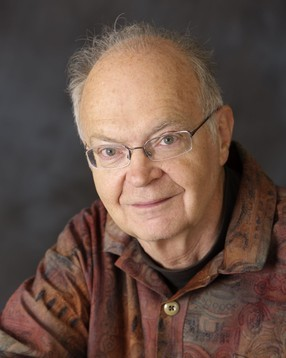
\includegraphics[width=.8\columnwidth]{support/images/Knuth.jpg}
    \end{column}
  \end{columns}
\end{frame}

\begin{frame}
  \frametitle{\LaTeX{}}
  \begin{columns}[c]
    \begin{column}{0.7\textwidth}
      \begin{center}
        \rmfamily\Huge
        \highlight[structure]{\LaTeX{}}
      \end{center}
      \begin{center}
        \parbox{0.75\textwidth}{
          \LaTeX{} 是最早在 1985 年由现就职于微软的 Leslie Lamport 开发的一种 \TeX{} \textbf{格式}\footnotemark,使用一些列宏和扩展宏包来简化 \TeX{} 的使用。现在由 \LaTeX{} Project 的成员维护。现在广泛使用的版本是 \LaTeXe{},最新的版本为 \LaTeX3(2020 年 10 月后默认内置)。
        }
      \end{center}
    \end{column}
    \begin{column}{0.3\textwidth}
      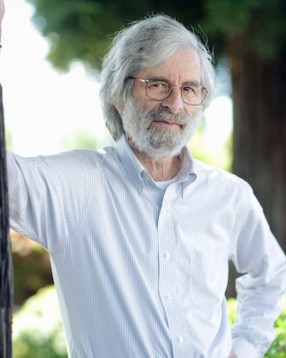
\includegraphics[width=.8\columnwidth]{support/images/Lamport.jpg}
    \end{column}
  \end{columns}
  \footnotetext{\hologo{ConTeXt} 也是一种 \TeX{} 格式 \link{https://www.contextgarden.net/}。}
\end{frame}

\begin{frame}
  \frametitle{程序}
  \begin{columns}[c]
    \begin{column}{0.7\textwidth}
      \begin{center}
        \rmfamily\Huge
        \highlight[structure]{\hologo{pdfLaTeX}}
      \end{center}
      \begin{center}
        \parbox{0.7\textwidth}{
          \hologo{pdfLaTeX} 是为了编译一个 \LaTeX{} 文档而运行的程序。实际上底层在运行一个叫 \hologo{pdfTeX} 的引擎,并预装了对应的 \LaTeX{} \textbf{格式}。为了利用临时文件,可能就需要多次运行程序。
        }
      \end{center}
    \end{column}
    \begin{column}{0.3\textwidth}
      \begin{block}{}
        \ttfamily\small
        > \highlight{pdflatex} main.tex\\
        This is pdfTeX, Version 3.141592653-
        2.6-1.40.23 (MiKTeX 21.10)\\
        entering extended mode\\
        \highlight{LaTeX2e} <2021-11-15>\\
        \highlight{L3} programming layer <2021-11-22>
      \end{block}
    \end{column}
  \end{columns}
\end{frame}

\begin{frame}
  \frametitle{引擎}
  \begin{columns}[c]
    \begin{column}{0.7\textwidth}
      \begin{center}
        \rmfamily\Huge
        \highlight[structure!70]{pdf}\hologo{La}\highlight[structure!70]{\TeX{}}
      \end{center}
      \begin{center}
        \parbox{0.7\textwidth}{
          pdf\TeX{} 是编译 \TeX{} 文档(以 \texttt{.tex} 结尾)的\textbf{引擎}---可以理解 \TeX{} 指令的\textbf{程序}。
        }
      \end{center}
    \end{column}
    \begin{column}{0.3\textwidth}
      \begin{block}{}
        \ttfamily\small
        > pdflatex main.tex\\
        This is \highlight[structure!70]{pdfTeX}, Version 3.141592653-
        2.6-1.40.23 (MiKTeX 21.10)
        entering extended mode\\
        LaTeX2e <2021-11-15>\\
        L3 programming layer <2021-11-22>
      \end{block}
    \end{column}
  \end{columns}
\end{frame}

\begin{frame}
  \frametitle{Unicode 引擎}
  \begin{table}
    \caption{主流 \hologo{(La)TeX} 程序
    \footnote{(u)p\TeX{} 是日语最常用的引擎,生成 \texttt{.dvi},支持 Unicode。}\footnote{Ap\TeX{} \link{https://github.com/clerkma/ptex-ng} 具有底层 CJK 支持,内联 Ruby,Color Emoji。}}
    \footnotesize
    \begin{stampbox}
      \begin{tabular}{c>{\raggedright}*{3}{p{3.5cm}}}
        \alert{引擎}     & \hologo{pdfTeX}   & \hologo{XeTeX}   & \hologo{LuaTeX}   \\
        \alert{程序}     & \hologo{pdfLaTeX} & \hologo{XeLaTeX} & \hologo{LuaLaTeX} \\
        \alert{特点}     & 直接生成 PDF,支持 micro-typography  & 支持 Unicode、OpenType 与复杂文字编排 (CTL) & 支持 Unicode,内联 Lua,支持 OpenType \\
      \end{tabular}
    \end{stampbox}
  \end{table}

  \begin{center}
    \parbox{.9\textwidth}{
      \hologo{pdfLaTeX} 不支持 Unicode。为了排版中文,大部分情况下 \faApple{}\,\faLinux{} 应当使用 \hologo{XeLaTeX},而 \hologo{LuaLaTeX} 速度相对较慢。\faWindows{} 可以在一些情况下使用 \hologo{pdfLaTeX}。
    }
  \end{center}
\end{frame}

% \begin{frame}
%   \paragraph{\hologo{pdfLaTeX}} \TeX{} 和 \LaTeX{} 被广泛使用之前,它们只需内置支持欧洲语言即可。在 Unicode 出现之前,\LaTeX{} 提供了许多种\textbf{文件编码}来允许很多语言的文字以原生的方式输入,\hologo{pdfLaTeX} 也只需要使用 8 位文件编码和 8 位字体。
% \end{frame}

\section{跑起来}
\begin{frame}
  \frametitle{发行版}
  \begin{table}
    \caption{\hologo{TeX} 发行版}
    \footnotesize
    \begin{stampbox}
      \begin{tabular}{c>{\raggedright}*{3}{p{3.2cm}}}
        \alert{发行版}     & \hologo{MiKTeX} \link{https://mirrors.sjtug.sjtu.edu.cn/ctan/systems/win32/miktex/setup/windows-x64/}   & \TeX{} Live \link{https://mirrors.sjtug.sjtu.edu.cn/ctan/systems/texlive/Images/}   & Mac\TeX{} \link{https://mirrors.sjtug.sjtu.edu.cn/ctan/systems/mac/mactex/}  \\[2pt]
        \alert{特点}      &  只安装必要文件,依赖用时更新  &  所有平台均可使用,每年发布一次 & Mac 系统专用,对 \TeX{} Live 的进一步打包 \\
        \alert{推荐平台}  & \faWindows  & \faLinux &  \faApple \\
      \end{tabular}
    \end{stampbox}
  \end{table}
  \begin{center}
    \parbox{.9\textwidth}{
      要让 \LaTeX{} 跑起来,核心就是要有一套 \TeX{} 发行版,来获取让 \LaTeX{} 工作所需的一组程序和文件。参考《一份简短的关于 \LaTeX{} 安装的介绍》\link{https://mirrors.sjtug.sjtu.edu.cn/ctan/info/install-latex-guide-zh-cn/install-latex-guide-zh-cn.pdf} 安装想使用的发行版。推荐使用发行版的最新版本\footnote{老版本 Linux 系统的包管理器自带 \TeX{} Live 发行版可能不是最新的 \link{https://repology.org/project/texlive/versions},尽量使用镜像安装,并手动将相关环境变量添加到路径 \link{https://www.tug.org/texlive/doc/texlive-zh-cn/texlive-zh-cn.pdf}。},并使用国内镜像。
    }
  \end{center}
\end{frame}

\begin{frame}[plain]
  \hbox to \textwidth{
    \hfil
    \vbox to 3cm{
      \hbox{
        \resizebox{3cm}{!}{
\includegraphics{support/examples/pics/sjtug}}
      }
    }
    \hfil
    \vbox to 3cm{
      \vfill
      \hbox{\Large\bfseries\color{structure} 稳定、快速、现代的镜像服务。}
      \vskip2pt
      \hbox{托管于华东教育网骨干节点上海交通大学。}
      \vfill
    }
    \hskip20pt
    \hfil
  }

  \begin{center}
    \parbox{0.8\textwidth}{
      推荐使用 SJTUG 软件镜像服务 \link{https://mirror.sjtu.edu.cn/},离得近,下得快。
      
      \begin{description}
        \footnotesize
        \item[\TeX{} Live]  {\ttfamily tlmgr option repository https://mirrors.sjtug.sjtu.edu.cn/CTAN/systems/texlive/tlnet}
        \item[\hologo{MiKTeX}] 在 \hologo{MiKTeX} Console 中设置镜像源为 \url{https://mirrors.sjtug.sjtu.edu.cn}
        \item[\faTelegram] 可以在 SJTUG 镜像站通知频道 \link{https://t.me/sjtug_mirrors_news} 获得更多信息,加入关联群组参与讨论。
      \end{description}
    }
  \end{center}
\end{frame}

\begin{frame}
  \frametitle{编辑器}
  \begin{table}
    \caption{开源编辑器推荐}
    \footnotesize
    \begin{stampbox}
      \begin{tabular}{c>{\raggedright}*{3}{p{3.5cm}}}
        \alert{编辑器}     & \begin{tabular}{c}Visual Studio Code\\ \LaTeX{} Workshop\end{tabular}  & \TeX{}studio & \TeX{}works \\[5pt]
        \alert{特点}      &  搭配 VS Code 使用非常方便,易扩展  & 可以使用大量的菜单选项输入代码块,用户友好 & 只提供基础的高亮与运行方法,发行版自带\footnote{Mac\TeX{} 打包的是 \TeX{}Shop 编辑器。} \\
      \end{tabular}
    \end{stampbox}
  \end{table}
  \begin{center}
    \parbox{.9\textwidth}{
      使用专为 \LaTeX{} 设计的编辑器将带来更多便利,因为它们往往会提供一键编译、内置 PDF 阅读器以及语法高亮等功能。几乎所有现代的 \LaTeX{} 编辑器都提供 Sync\TeX{} 这一强大的功能,以在 PDF 和代码间对应跳转。
    }
  \end{center}
\end{frame}

\begin{frame}
  \frametitle{在线平台}
  \begin{table}
    \caption{在线协作平台推荐}
    \footnotesize
    \begin{stampbox}
      \begin{tabular}{c>{\raggedright}*{2}{p{4cm}}}
        \alert{在线平台}     & Overleaf \link{https://www.overleaf.com/}  & 交大 \LaTeX{} 助手 \link{https://latex.sjtu.edu.cn/} \\[2pt]
        \alert{特点}      & 最流行的在线平台,提供大量的模板,但国内访问慢 & 校内平台,隐私保护有保障,共享项目限制少 \\
      \end{tabular}
    \end{stampbox}
  \end{table}
  \begin{center}
    \parbox{.9\textwidth}{
      在线平台允许你直接在网页中编辑文档,无需本地安装即可在后台运行 \LaTeX{},并显示生成的 PDF。可以参照 Overleaf 官方文档学习如何使用在线平台 \link{https://www.overleaf.com/learn}。
    }
  \end{center}
\end{frame}

\section{基本结构}
\begin{frame}[fragile]%
  \frametitle{文档部件}
  \begin{columns}[c]
    \begin{column}{0.4\textwidth}
      \only<1>{
        \cmd{documentclass} 命令加载了\textbf{文档类}。\cls{article} 是由 \LaTeX{} 提供的用于排版短文档的基本文档类。
        \begin{description}
          \footnotesize
          \item[\cls{article}] 不包含章的短文档
          \item[\cls{report}] 含有章的单面印刷文档
          \item[\cls{book}] 含有章的双面印刷文档
          \item[\cls{beamer}] 幻灯片
        \end{description}
      }

      \only<2>{
        \env{document} 环境用于指示文档主体的范围。\LaTeX{} 还有其他的使用 \cmd{begin} 和 \cmd{end} 的搭配,我们称这些为\textbf{环境}。它们将用来设定局部格式命令\footnotemark。
      }

      \only<3>{
        \includepdflarge{support/examples/enminimal.pdf}
      }
    \end{column}
    \begin{column}{0.6\textwidth}
      \begin{codeblock}[]{排版英文最简示例}
|\highlightline<1>|\documentclass{article}
|\highlightline<2>|\begin{document}
|\highlightline<3>|  Together for a Shared Future
|\highlightline<2>|\end{document}
      \end{codeblock}
    \end{column}
  \end{columns}

  \only<2>{\footnotetext{环境实际上是一个组,只不过通过语义化的形式预装了对应的格式命令。普通的组可以直接使用一对大括号之间的内容 \{$\cdots$\} 表示。}}
\end{frame}

\section{扩展}
\begin{frame}[fragile]%
  \frametitle{中文排版}
  \begin{columns}[c]
    \begin{column}{0.4\textwidth}

      \only<1>{
        \cmd{usepackage} 用于使用宏包以向 \LaTeX{} 添加或修改功能,需要在\textbf{导言区}调用。
        这里使用 \pkg{ctex} 宏集以获得中文支持。其调用底层因不同的引擎而不同。
        \begin{center}
          \footnotesize
          \begin{tabular}{c*{3}{c}}
            \alert{引擎}     & \hologo{pdfTeX}   & \hologo{XeTeX}   & \hologo{LuaTeX}   \\
            \alert{程序}     & \hologo{pdfLaTeX} & \hologo{XeLaTeX} & \hologo{LuaLaTeX} \\
            \alert{宏包}     & CJK\footnotemark & xeCJK & luatexja \\
            \alert{封装}     & \multicolumn{3}{c}{ctex} \\
          \end{tabular}
        \end{center}
        \vspace{-1cm}
      }

      \only<2>{
        \CTeX{} 建议对于之前提到的常规文档类,最佳实践是使用该宏集提供的四种中文文档类,以对特定类型提供额外的中文排版适配。
        \begin{center}
          \footnotesize
          \begin{tabular}{cc}
            \cls{ctexart} & \cls{ctexrep} \\
            \cls{ctexbook} & \cls{ctexbeamer} \\
          \end{tabular}
        \end{center}
      }

      \only<3>{
        \includepdflarge{support/examples/cnminimal.pdf}
      }

      \only<4>{
        大部分情况下,你都不应当在 \LaTeX{} 中强制断行:你几乎只是想另起一段,或者是想在段落之间添加空行(使用 \pkg{parskip} 宏包就可实现)。
        只有\alert{很少的}情况下你需要使用 \textbackslash{}\textbackslash{} 来另起一行而不另起一段(强制断行仍在同一段)。
      }
    \end{column}
    \begin{column}{0.6\textwidth}
      \begin{codeblock}[]{排版中文\only<2->{最佳实践}}
|\highlightline<2>|\documentclass{|\only<1>{article}\only<2->{ctexart}|}
|\only<1>{\highlightline\textbackslash{}usepackage\{ctex\}\hfill\color{structure}\% 导言区}|
\begin{document}
|\highlightline<3>|    一起向未来
|\highlightline<4>|
  Together for a Shared Future
\end{document}
      \end{codeblock}
    \end{column}
  \end{columns}
  \only<1>{\footnotetext{ctex 在 \faApple\,\faLinux{} 上已经不可以使用 \hologo{pdfLaTeX} 编译,以及在 \faWindows{} 上使用该引擎也会变更自动间距调整等功能的默认行为。}}
\end{frame}

\section{设定格式}
\begin{frame}[fragile]%
  \frametitle{字体样式}
  \begin{columns}
    \begin{column}{0.4\textwidth}
      \only<1>{
        \includepdflarge{support/examples/fontstyle.pdf}
      }

      \only<2>{
        可以使用显式样式设定命令对小段做加粗、斜体、等宽等等的处理。
        \begin{center}
          \footnotesize
          \begin{tabular}{rl}
            \cmd{textrm} & \textrm{衬线} \\
            \cmd{textbf} & \textbf{加粗} \\
            \cmd{textit} & \kaishu 斜体 \\
            \cmd{texttt} & \texttt{等宽} \\
            \cmd{textsf} & \textsf{无衬线} \\
            \cmd{textsc} & \textsc{Small Caps} \\
            \cmd{textsl} & \textsl{Slanted} \\
          \end{tabular}
        \end{center}
      }

      \only<3>{
        与 Word 不同的是,\LaTeX{} 一般情况下并不需要使用上面的显式命令,而是采用逻辑标记的方法,
        比如 \cmd{emph} 可以强调文字,以及下面将要提到的目次命令(第 \ref{sectioning} 页)。
        这样可以统一管理格式。
      }
    \end{column}
    \begin{column}{0.6\textwidth}
      \begin{codeblock}[]{样式}
\documentclass{ctexart}
\begin{document}
|\highlightline<2>|  \textbf{||一起向未来}

|\highlightline<3>|  \emph{Together for a Shared Future}
\end{document}
      \end{codeblock}
    \end{column}
  \end{columns}
\end{frame}

\begin{frame}[fragile]%
  \frametitle{\only<1-2>{字体大小}\only<3>{字体样式}}
  \begin{columns}
    \begin{column}{0.4\textwidth}
      \only<1>{
        \includepdflarge{support/examples/fontsize.pdf}
      }

      \only<2>{
        同样地,你也可以显式地设定字体大小,但是这种命令会更改行文设置,所以需要使用一个组来限定作用范围\footnotemark。
        \begin{center}
          \footnotesize
          \begin{tabular}{rl}
            \cmd{tiny} & \tiny 极小 \\
            \cmd{scriptsize} & \scriptsize 角标大小  \\
            \cmd{footnotesize} & \footnotesize 脚注大小 \\
            \cmd{small} & \small 小 \\
            \cmd{normalsize} & \normalsize 正常大小 \\
            \cmd{large} & \large 大 \\
            \cmd{huge} & \Huge 巨大 \\
          \end{tabular}
        \end{center}
      }

      \only<3>{
        也可以使用字体样式对应的更改字体设置的命令,这对于大段文段的设置而言也是很方便的。
        \begin{center}
          \footnotesize
          \begin{tabular}{ll}
            \cmd{textrm} & \cmd{rmfamily}\\
            \cmd{texttt} & \cmd{ttfamily}\\
            \cmd{textsf} & \cmd{sffamily}\\
            \cmd{textbf} & \cmd{bfseries}\\
            \cmd{textit} & \cmd{itshape}\\
            \cmd{textsc} & \cmd{scshape}\\
            \cmd{textsl} & \cmd{slshape}\\
          \end{tabular}
        \end{center}
      }
    \end{column}
    \begin{column}{0.6\textwidth}
      \begin{codeblock}[]{大小}
\documentclass{ctexart}
\begin{document}
|\highlightline<2>|  {\bfseries\Large 一起向未来\par}
|\highlightline<3>|  {\itshape Together for a Shared Future}
\end{document}
      \end{codeblock}
    \end{column}
  \end{columns}

  \only<2>{\footnotetext{注意最后显式地使用 \cmd{par} 在改回大小前结束该段,否则会导致下一行的行间距异常!}}
\end{frame}

\section{逻辑结构}
\begin{frame}[fragile]
  \frametitle{列表}
  \begin{columns}
    \begin{column}{0.35\textwidth}
      \begin{codeblock}[]{无序列表}
\documentclass{ctexart}
\begin{document}
|\highlightline|  \begin{itemize}
    \item 第一项
    \item 第二项
    \item 第三项
|\highlightline|  \end{itemize}
\end{document}
      \end{codeblock}
    \end{column}
    \begin{column}{0.35\textwidth}
      \begin{codeblock}[]{有序列表}
\documentclass{ctexart}
\begin{document}
|\highlightline|  \begin{enumerate}
    \item 第一项
    \item 第二项
    \item 第三项
|\highlightline|  \end{enumerate}
\end{document}
      \end{codeblock}
    \end{column}
    \begin{column}{0.35\textwidth}
      \begin{codeblock}[]{描述列表}
\documentclass{ctexart}
\begin{document}
|\highlightline|  \begin{description}
    \item[||第一] 文本
    \item[||第二] 文本
    \item[||第三] 文本  
|\highlightline|  \end{description}
\end{document}
      \end{codeblock}
    \end{column}
  \end{columns}
\end{frame}

%更深的列表技巧,定理环境等

\begin{frame}
  \frametitle{列表}
  \begin{columns}
    \begin{column}{0.35\textwidth}
      \includepdflarge{support/examples/unordered.pdf}
    \end{column}
    \begin{column}{0.35\textwidth}
      \includepdflarge{support/examples/ordered.pdf}
    \end{column}
    \begin{column}{0.35\textwidth}
      \includepdflarge{support/examples/description.pdf}
    \end{column}
  \end{columns}
\end{frame}

\begin{frame}[fragile,label=sectioning]%
  \frametitle{目次结构}
  \begin{columns}
    \begin{column}{0.4\textwidth}
      \LaTeX{} 可以使用目次命令将文档划分层级\footnotemark,并自动设定对应字体样式和大小。
      \begin{center}
        \footnotesize
        \begin{tabular}{rll}
          命令 & 含义 & 层次 \\
          \cmd{chapter} & 章\footnotemark & \sout{0} \\
          \cmd{section} & 节 & 1 \\
          \cmd{subsection} & 小节 & 2 \\
          \cmd{subsubsection} & 小小节 & 3 \\
        \end{tabular}
      \end{center}
    \end{column}
    \begin{column}{0.6\textwidth}
      \begin{codeblock}[]{目次}
\documentclass{ctexart}
\begin{document}
|\highlightline|  \section{||概念}
|\highlightline|  \subsection{\LaTeX{}}
  \LaTeX{} 是一个用以排版高质量作品的文档准备系统。
\end{document}
      \end{codeblock}
    \end{column}
  \end{columns}
  \footnotetext{章这一级只在 \cls{report} 和 \cls{book} 文档类(包括对应的中文文档类)有定义。还有不常用的 \cmd{part} (0@\cls{article}/-1@\cls{report}\&\cls{book}\&\cls{beamer}) 以及更低层次的 \cmd{paragraph} (4) 与 \cmd{subparagraph} (5)。 }
\end{frame}

\begin{frame}[fragile]%
  \frametitle{组织文档}
  \begin{columns}
    \begin{column}{0.4\textwidth}

      \only<1>{
        \cmd{tableofcontents} 用来生成对于目次命令的目录。如果你想设定显示到哪个层级,在这个命令前使用 \cmd{setcounter\{tocdepth\}\{层次\}}

        如果你想在目录中使用更短的标题:

            \cmd{section[短标题]\{长标题\}}

        如果你想让本目次的标题不显示在目录中:

            \cmd{section*\{目录没这个标题\}}
      }

      \only<2>{
        对于大型文档而言,使用多个文件管理源文件通常是更方便的。而 \cmd{include} 和 \cmd{input} 都以相对路径的方式插入其他 \TeX{} 文档。
        区别在于,\cmd{include} 命令会从新页开始并做一些内部调整,这基本上只对 \pkg{chapter} 这一级有用。而 \cmd{input} 会原样插入源代码。
      }

      \only<3>{
        但是 \cmd{include} 插入的文档可以使用 \cmd{includeonly} 管理当前要排印哪一部分的内容,利用所有章节辅助文件的同时,减少编译时间并专注于该部分的内容。
      }
    \end{column}
    \begin{column}{0.6\textwidth}
      \begin{codeblock}[]{主文档}
\documentclass{ctexrep}
|\highlightline<3>|\includeonly{learnlatex,sjtuthesis}
\begin{document}
|\highlightline<1>|  \tableofcontents
|\only<2-3>{\highlightline}|  % !TeX root = ../../latex-talk.tex

\part{学习 \LaTeX{}}
% FIXME: footnote fault numbering
% FIXME: section pop up in navigation in advance

\begin{frame}
  \frametitle{本部分主要参考}
  \begin{bibliolist}{00}
    \onlineitem 陈晟祺~等.
    \newblock 如何使用 \LaTeX\ 排版论文[EB/OL].
    \newblock 2021. \url{https://github.com/tuna/thulib-latex-talk}.

    \onlineitem 曾祥东.
    \newblock 现代 \LaTeX\ 入门讲座[EB/OL].
    \newblock 2022. \url{https://github.com/stone-zeng/latex-talk}.

    \onlineitem \LaTeX\ Project.
    \CTeX\ 开发小组~译.
    \newblock learnlatex.org[EB/OL].
    \newblock 2022. \url{https://github.com/CTeX-org/learnlatex.github.io}.
  
    \onlineitem \textsc{Oetiker T}, \textsc{Partl H}, \textsc{Hyna I}, \textsc{Schlegl E}.
    \CTeX\ 开发小组~译.
    \newblock 一份(不太)简短的 \LaTeXe{} 介绍:或 111 分钟了解 \LaTeXe{}[EB/OL]. \newblock\newblock 2021.
    \url{https://ctan.org/pkg/lshort-zh-cn}.
  \end{bibliolist}

  \note{推荐大家去阅读这些入门材料。}
\end{frame}

\begin{frame}[plain]
  \vfil
  \begin{center}
    \href{https://learnlatex.org}{
      \rmfamily
      Learn\,\lower1ex\hbox{\Huge\LaTeX{}}.org
    }
  \end{center}
  \vfil
  \begin{center}
    \parbox{0.75\linewidth}{
      Learn\LaTeX{}.org 提供了解 \LaTeX{} 的 16 篇简短的教程,并包含了一些可以在线运行的示例,可以通过亲自动手查看实验效果。本部分主要参考由 \CTeX{}-org 提供的中文翻译版本 \link{https://github.com/CTeX-org/learnlatex.github.io/tree/zh-Hans/zh-Hans/}。
    }
  \end{center}
  \vfil
  \note{这一部分主要参考了 Learn\LaTeX{}.org 的系列教程,内容简洁,适合入门,符合
  教育学观念 \link{https://www.tug.org/TUGboat/tb41-2/tb128reviews-learnlatex.pdf},
  并参考由 \CTeX{}-org 提供的中文翻译版本
  \link{https://github.com/CTeX-org/learnlatex.github.io/tree/zh-Hans/zh-Hans/}。
  如果你认为下面一个小时的入门教程没有讲得非常细致的话,
  欢迎直接阅读这个网站的全文。}
\end{frame}

\begin{shadedsection}

\section{是什么}
\begin{frame}
  \frametitle{\TeX{}}
  \begin{columns}[c]
    \begin{column}{0.7\textwidth}
      \begin{center}
        \rmfamily\Huge
        \hologo{La}\highlight[structure!70]{\TeX{}}
      \end{center}
      \begin{center}
        \parbox{0.75\textwidth}{
          \TeX{} 是由斯坦福大学教授高德纳
          (Donald E.~Knuth)于 1977 年开始开发的排版引擎。目前仍在更新,最新版本号为 3.141592653 \link{https://tug.org/TUGboat/tb42-1/tb130knuth-tuneup21.pdf}。
        }
      \end{center}
    \end{column}
    \begin{column}{0.3\textwidth}
      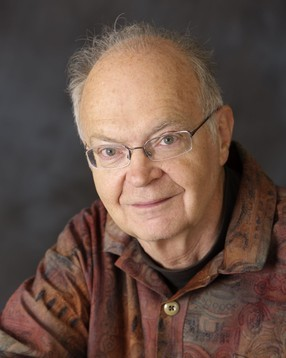
\includegraphics[width=.8\columnwidth]{support/images/Knuth.jpg}
    \end{column}
  \end{columns}
  \note{\emph{这一部分背景介绍大家可以了解一下,暂时跳过。}
  \LaTeX{} 这个词由两个部分组成,\hologo{La} 和 \TeX{}。那我们首先了解一下 \TeX{} 是什么。
  \TeX{} 是由斯坦福大学的教授高德纳于 1977 年开始开发的排版引擎,它已经有三十多年的历史了,
  目前仍在更新,版本号(3.141592653)将会趋近于 $\pi$ 的取值,高德纳最近还在给 \textsl{TUGBoat} 写稿子
  \link{https://tug.org/TUGboat/tb42-1/tb130knuth-tuneup21.pdf},
  关于 \TeX{} 今年又做了哪些改进。}
\end{frame}

\begin{frame}
  \frametitle{\LaTeX{}}
  \begin{columns}[c]
    \begin{column}{0.7\textwidth}
      \begin{center}
        \rmfamily\Huge
        \highlight[structure]{\LaTeX{}}
      \end{center}
      \begin{center}
        \parbox{0.75\textwidth}{
          \LaTeX{} 是最早在 1985 年由现就职于微软的 Leslie Lamport 开发的一种 \TeX{} \textbf{格式}\footnotemark,使用一些列宏和扩展宏包来简化 \TeX{} 的使用。现在由 \LaTeX{} Project 的成员维护。现在广泛使用的版本是 \LaTeXe{},最新的版本为 \LaTeX3(2020 年 10 月后默认内置)。
        }
      \end{center}
    \end{column}
    \begin{column}{0.3\textwidth}
      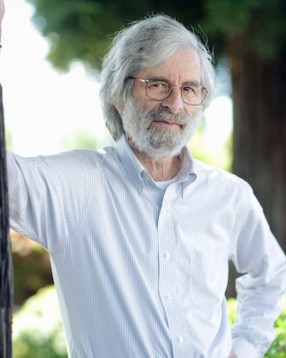
\includegraphics[width=.8\columnwidth]{support/images/Lamport.jpg}
    \end{column}
  \end{columns}
  \footnotetext{\hologo{ConTeXt} 也是一种 \TeX{} 格式 \link{https://www.contextgarden.net/}。}
  \note{\emph{这一部分的背景介绍大家可以了解一下,暂时跳过。}
  \LaTeX{} 是最早由现就职于微软的 Leslie Lamport 开发的一种 \TeX{} 格式(与其对标的是
  \hologo{ConTeXt}\link{https://www.contextgarden.net/}),主要也是为了简化 \TeX{} 的使用。
  现在主要由 \LaTeX{} 开发组维护,现在广泛使用的版本是 \LaTeXe{},最新的版本为 \LaTeX3,
  在 2020 年 10 月后默认内置,所以要尽可能使用较新的发行版,以充分发挥其功能。}
\end{frame}

\begin{frame}
  \frametitle{程序}
  \begin{columns}[c]
    \begin{column}{0.7\textwidth}
      \begin{center}
        \rmfamily\Huge
        \highlight[structure]{\hologo{pdfLaTeX}}
      \end{center}
      \begin{center}
        \parbox{0.7\textwidth}{
          \hologo{pdfLaTeX} 是为了编译一个 \LaTeX{} 文档而运行的程序。实际上底层在运行一个叫 \hologo{pdfTeX} 的引擎,并预装了对应的 \LaTeX{} \textbf{格式}。为了利用临时文件,可能就需要多次运行程序。
        }
      \end{center}
    \end{column}
    \begin{column}{0.3\textwidth}
      \begin{block}{}
        \ttfamily\small
        > \highlight{pdflatex} main.tex\\
        This is pdfTeX, Version 3.141592653-
        2.6-1.40.23 (MiKTeX 21.10)\\
        entering extended mode\\
        \highlight{LaTeX2e} <2021-11-15>\\
        \highlight{L3} programming layer <2021-11-22>
      \end{block}
    \end{column}
  \end{columns}
  \note{\hologo{pdfLaTeX} 是为了编译一个 \LaTeX{} 文档而运行的程序。}
\end{frame}

\begin{frame}
  \frametitle{引擎}
  \begin{columns}[c]
    \begin{column}{0.7\textwidth}
      \begin{center}
        \rmfamily\Huge
        \highlight[structure!70]{pdf}\hologo{La}\highlight[structure!70]{\TeX{}}
      \end{center}
      \begin{center}
        \parbox{0.7\textwidth}{
          pdf\TeX{} 是编译 \TeX{} 文档(以 \texttt{.tex} 结尾)的\textbf{引擎}---可以理解 \TeX{} 指令的\textbf{程序}。
        }
      \end{center}
    \end{column}
    \begin{column}{0.3\textwidth}
      \begin{block}{}
        \ttfamily\small
        > pdflatex main.tex\\
        This is \highlight[structure!70]{pdfTeX}, Version 3.141592653-
        2.6-1.40.23 (MiKTeX 21.10)
        entering extended mode\\
        LaTeX2e <2021-11-15>\\
        L3 programming layer <2021-11-22>
      \end{block}
    \end{column}
  \end{columns}
  \note{实际上底层在运行一个叫 \hologo{pdfTeX} 的引擎,并预装了对应的 \LaTeX{} 格式。}
\end{frame}

\begin{frame}[label={frame:engine}]
  \frametitle{Unicode 引擎}
  \begin{table}
    \caption{主流 \hologo{(La)TeX} 程序
    \footnote{(u)p\TeX{} 是日语最常用的引擎,生成 \texttt{.dvi},支持 Unicode。}\footnote{Ap\TeX{} \link{https://github.com/clerkma/ptex-ng} 具有底层 CJK 支持,内联 Ruby,Color Emoji。}}
    \footnotesize
    \begin{stampbox}
      \begin{tabular}{c>{\raggedright}*{3}{p{3.5cm}}}
        \alert{引擎}     & \hologo{pdfTeX}   & \hologo{XeTeX}   & \hologo{LuaTeX}   \\
        \alert{程序}     & \hologo{pdfLaTeX} & \hologo{XeLaTeX} & \hologo{LuaLaTeX} \\
        \alert{特点}     & 直接生成 PDF,支持 micro-typography  & 支持 Unicode、OpenType 与复杂文字编排 (CTL) & 支持 Unicode,内联 Lua,支持 OpenType \\
      \end{tabular}
    \end{stampbox}
  \end{table}

  \begin{center}
    \parbox{.9\textwidth}{
      \hologo{pdfLaTeX} 不支持 Unicode。为了排版中文,大部分情况下 \faApple{}\,\faLinux{} 应当使用 \hologo{XeLaTeX},而 \hologo{LuaLaTeX} 速度相对较慢。\faWindows{} 可以在一些情况下使用 \hologo{pdfLaTeX}。
    }
  \end{center}
  \note{当然为了排版中文,已经不再推荐使用 \hologo{pdfLaTeX} 了,应该使用 
  \hologo{XeLaTeX} 或者 \hologo{LuaLaTeX},当然后者的速度还是相对较慢,
  它们支持 Unicode 编码,并可以使用 OpenType 字体的全部功能。
  当然 \faWindows{} 平台下在某些追求速度的情况下,
  还是可以试着使用 \hologo{pdfLaTeX} 的。
  
  \hologo{LuaLaTeX} 理想情况下不慢,但是使用一些宏包后会破坏理想状态,
  也会因配置产生不同的结果,不同的操作系统在 I/O 速度上的不同也会导致不同的时间。

  \hologo{pdfLaTeX} 也支持,只不过需要先生成 tfm \TeX{} 字体度量文件,后续使用 \TeX{} 
  自身的配置方法,只能使用 7 比特或 8 比特字体。}
\end{frame}

% \begin{frame}
%   \paragraph{\hologo{pdfLaTeX}} \TeX{} 和 \LaTeX{} 被广泛使用之前,它们只需内置支持欧洲语言即可。在 Unicode 出现之前,\LaTeX{} 提供了许多种\textbf{文件编码}来允许很多语言的文字以原生的方式输入,\hologo{pdfLaTeX} 也只需要使用 8 位文件编码和 8 位字体。
% \end{frame}

\section{跑起来}
\begin{frame}
  \frametitle{发行版}
  \begin{table}
    \caption{\hologo{TeX} 发行版}
    \footnotesize
    \begin{stampbox}
      \begin{tabular}{c>{\raggedright}*{3}{p{3.2cm}}}
        \alert{发行版}     & \hologo{MiKTeX} \link{https://mirrors.sjtug.sjtu.edu.cn/ctan/systems/win32/miktex/setup/windows-x64/}   & \TeX{} Live \link{https://mirrors.sjtug.sjtu.edu.cn/ctan/systems/texlive/Images/}   & Mac\TeX{} \link{https://mirrors.sjtug.sjtu.edu.cn/ctan/systems/mac/mactex/}  \\[2pt]
        \alert{特点}      &  只安装必要文件,依赖用时更新  &  所有平台均可使用,每年发布一次 & Mac 系统专用,对 \TeX{} Live 的进一步打包 \\
        \alert{推荐平台}  & \faWindows  & \faLinux &  \faApple \\
      \end{tabular}
    \end{stampbox}
  \end{table}
  \begin{center}
    \parbox{.9\textwidth}{
      要让 \LaTeX{} 跑起来,核心就是要有一套 \TeX{} 发行版,来获取让 \LaTeX{} 工作所需的一组程序和文件。参考《一份简短的关于 \LaTeX{} 安装的介绍》\link{https://mirrors.sjtug.sjtu.edu.cn/ctan/info/install-latex-guide-zh-cn/install-latex-guide-zh-cn.pdf} 安装想使用的发行版。推荐使用发行版的最新版本\footnote{老版本 Linux 系统的包管理器自带 \TeX{} Live 发行版可能不是最新的 \link{https://repology.org/project/texlive/versions},尽量使用镜像安装,并手动将相关环境变量添加到路径 \link{https://www.tug.org/texlive/doc/texlive-zh-cn/texlive-zh-cn.pdf}。},并使用国内镜像。
    }
  \end{center}
  \note{要让 \LaTeX{} 跑起来,核心就是要有一套 \TeX{} 发行版,来获取让 
  \LaTeX{} 工作所需的一组程序和文件。参考《一份简短的关于 \LaTeX{} 安装的介绍》
  安装想使用的发行版,里面介绍了 \faWindows{}, \faApple{}, \faLinux{}, WSL 等系统上
  \TeX{} Live 的安装,非常全面,一步一步做就可以成功安装。目前最新的 \TeX{} Live 版本为
  2022,\SJTUThesis{} 用户不应当安装 \TeX{} Live 2020 以下的版本(后面会讲)。
  
  事实上,我认为这几个发行版各有操作系统偏好,虽然前两者是跨平台的。

  \hologo{MiKTeX} 对 Windows 用户较为友好,安装简单,占用空间不大,安装时间短,
  而且有完整的安装与卸载程序。可以给大家看一下 \hologo{MiKTeX} Console 的情况。

  \TeX{} Live 更符合 Linux 的更新传统。老版本 Linux 系统的包管理器自带 \TeX{} Live
  发行版可能不是最新的(到时间也会锁定依赖库的版本),尽量使用镜像安装(当然也推荐使用最新的
  Linux 发行版,这样它的版本也就一直是最新的),并手动将相关环境变量添加到路径。

  Mac\TeX{} 发行版有 pkg 安装包封装,并且附带了 \TeX{}Shop 基本编辑软件,更加适合 Mac OS。
  我用下来的话,感觉除了 \TeX{} Live Utility 外都有点过时了。}
\end{frame}

\begin{frame}[plain]
  \hbox to \textwidth{
    \hfil
    \vbox to 3cm{
      \hbox{
        \resizebox{3cm}{!}{
\includegraphics{support/examples/pics/sjtug}}
      }
    }
    \hfil
    \vbox to 3cm{
      \vfill
      \hbox{\Large\bfseries\color{structure} 稳定、快速、现代的镜像服务。}
      \vskip2pt
      \hbox{托管于华东教育网骨干节点上海交通大学。}
      \vfill
    }
    \hskip20pt
    \hfil
  }

  \begin{center}
    \parbox{0.8\textwidth}{
      推荐使用 SJTUG 软件镜像服务 \link{https://mirror.sjtu.edu.cn/},离得近,下得快。
      
      \begin{description}
        \footnotesize
        \item[\TeX{} Live]  {\ttfamily tlmgr option repository https://mirrors.sjtug.sjtu.edu.cn/CTAN/systems/texlive/tlnet}
        \item[\hologo{MiKTeX}] 在 \hologo{MiKTeX} Console 中设置镜像源为 \url{https://mirrors.sjtug.sjtu.edu.cn}
        \item[\faTelegram] 可以在 SJTUG 镜像站通知频道 \link{https://t.me/sjtug_mirrors_news} 获得更多信息,加入关联群组参与讨论。
      \end{description}
    }
  \end{center}
  \note{说到镜像,像后两者的安装包都很大(4GB 左右),由于一些原因,不采用镜像的话不知道要下到什么时候,对下载速度的要求高;
  而 \hologo{MiKTeX} 需要随时更新,宏包大小颗粒度大,对延迟的要求高。
  那么采用 SJTUG 镜像源将同时解决这两个问题,位于图信大楼的机房,凭借校内的高速网络,稳定快速下载,
  现在由 LightQuantum 维护的镜像站欢迎大家的使用,主页上还有更多的其他镜像可供使用,加入 Telegram 群组参与讨论。}
\end{frame}

\begin{frame}
  \frametitle{编辑器}
  \begin{table}
    \caption{开源编辑器推荐}
    \footnotesize
    \begin{stampbox}
      \begin{tabular}{c>{\raggedright}*{3}{p{3.5cm}}}
        \alert{编辑器}     & \begin{tabular}{c}Visual Studio Code \link{https://code.visualstudio.com}\\ \LaTeX{} Workshop\end{tabular}  & \TeX{}studio \link{https://texstudio.org} & \TeX{}works \\[5pt]
        \alert{特点}      &  搭配 VS Code 使用非常方便,易扩展  & 可以使用大量的菜单选项输入代码块,用户友好 & 只提供基础的高亮与运行方法,发行版自带\footnote{Mac\TeX{} 打包的是 \TeX{}Shop 编辑器。} \\
      \end{tabular}
    \end{stampbox}
  \end{table}
  \begin{center}
    \parbox{.9\textwidth}{
      使用专为 \LaTeX{} 设计的编辑器将带来更多便利,因为它们往往会提供一键编译、内置 PDF 阅读器以及语法高亮等功能。几乎所有现代的 \LaTeX{} 编辑器都提供 Sync\TeX{} 这一强大的功能,以在 PDF 和代码间对应跳转。
    }
  \end{center}
  \note{编辑器的种类很多,我无法一一列举,但是对编写 \TeX{} 常用的开源编辑器我推荐这三个。
  其中 \TeX{}studio 的安装包可能下得有点慢。这里我对这些编辑器都演示一下,初学者我更推荐使用
  \TeX{} studio 编辑器,如果平时就码很多代码的话,我更推荐使用 VS Code 加插件这种方式。
  
  使用专为 \LaTeX{} 设计的编辑器将带来更多便利,因为它们往往会提供一键编译、内置 PDF 阅读器
  以及语法高亮等功能。几乎所有现代的 \LaTeX{} 编辑器都提供 Sync\TeX{} 这一强大的功能
  (VS Code 的方法是 Ctrl + 某处,Overleaf 的方法是直接双击),以在 PDF 和代码间对应跳转。
  当然如果你不喜欢使用这种 GUI 编辑器,\TeX{} 文档本身就是纯文本,对 Vim, Emacs 等终端用户
  也很友好。}
\end{frame}

\begin{frame}
  \frametitle{在线平台}
  \begin{table}
    \caption{在线协作平台推荐}
    \footnotesize
    \begin{stampbox}
      \begin{tabular}{c>{\raggedright}*{2}{p{4cm}}}
        \alert{在线平台}     & Overleaf \link{https://www.overleaf.com/}  & 交大 \LaTeX{} 助手 \link{https://latex.sjtu.edu.cn/} \\[2pt]
        \alert{特点}      & 最流行的在线平台,提供大量的模板,但国内访问慢 & 校内平台,隐私保护有保障,共享项目限制少 \\
      \end{tabular}
    \end{stampbox}
  \end{table}
  \begin{center}
    \parbox{.9\textwidth}{
      在线平台允许你直接在网页中编辑文档,无需本地安装即可在后台运行 \LaTeX{},并显示生成的 PDF。可以参照 Overleaf 官方文档学习如何使用在线平台 \link{https://www.overleaf.com/learn}。
    }
  \end{center}
  \note{当然使用在线平台省去了安装发行版的麻烦,这里列出两种在线写作平台。

  如果有数据合规需求的话,可以考虑使用由网络信息中心维护的交大 \LaTeX{} 助手,最近更新了 \TeX{} Live 2022,还是很不错的。

  当然国内还有 \TeX{} Page \link{https://www.texpage.com/},Slagger \link{https://www.slager.cn/} 等。
  一般来讲,这种平台使用的都是 Linux 操作系统,所以在排版中文的时候考虑将编译引擎更改为 \hologo{XeLaTeX},
  学习如何使用在线平台参见 Overleaf 的官方文档 \link{https://www.overleaf.com/learn}。}
\end{frame}

\section{基本结构}
\begin{frame}[fragile]%
  \frametitle{文档部件}
  \begin{columns}[c]
    \begin{column}{0.4\textwidth}
      \only<1>{
        \cmd{documentclass} 命令加载了\textbf{文档类}。\cls{article} 是由 \LaTeX{} 提供的用于排版短文档的基本文档类。
        \begin{description}
          \footnotesize
          \item[\cls{article}] 不包含章的短文档
          \item[\cls{report}] 含有章的单面印刷文档
          \item[\cls{book}] 含有章的双面印刷文档
          \item[\cls{beamer}] 幻灯片
        \end{description}
      }

      \only<2>{
        \env{document} 环境用于指示文档主体的范围。\LaTeX{} 还有其他的使用 \cmd{begin} 和 \cmd{end} 的搭配,我们称这些为\textbf{环境}。它们将用来设定局部格式命令\footnotemark。
      }

      \only<3>{
        \includepdflarge{support/examples/enminimal.pdf}
      }
    \end{column}
    \begin{column}{0.6\textwidth}
      \begin{codeblock}[]{排版英文最简示例}
|\highlightline<1>|\documentclass{article}
|\highlightline<2>|\begin{document}
|\highlightline<3>|  Together for a Shared Future
|\highlightline<2>|\end{document}
      \end{codeblock}
    \end{column}
  \end{columns}

  \only<2>{\footnotetext{环境实际上是一个组,只不过通过语义化的形式预装了对应的格式命令。普通的组可以直接使用一对大括号之间的内容 \{$\cdots$\} 表示。}}
\end{frame}

\section{扩展}
\begin{frame}[fragile]%
  \frametitle{中文排版}
  \begin{columns}[c]
    \begin{column}{0.4\textwidth}

      \only<1>{
        \cmd{usepackage} 用于使用宏包以向 \LaTeX{} 添加或修改功能,需要在\textbf{导言区}调用。
        这里使用 \pkg{ctex} 宏集以获得中文支持。其调用底层因不同的引擎而不同。
        \begin{center}
          \footnotesize
          \begin{tabular}{c*{3}{c}}
            \alert{引擎}     & \hologo{pdfTeX}   & \hologo{XeTeX}   & \hologo{LuaTeX}   \\
            \alert{程序}     & \hologo{pdfLaTeX} & \hologo{XeLaTeX} & \hologo{LuaLaTeX} \\
            \alert{宏包}     & CJK\footnotemark & xeCJK & luatexja \\
            \alert{封装}     & \multicolumn{3}{c}{ctex} \\
          \end{tabular}
        \end{center}
        \vspace{-1cm}
      }

      \only<2>{
        \CTeX{} 建议对于之前提到的常规文档类,最佳实践是使用该宏集提供的四种中文文档类,以对特定类型提供额外的中文排版适配。
        \begin{center}
          \footnotesize
          \begin{tabular}{cc}
            \cls{ctexart} & \cls{ctexrep} \\
            \cls{ctexbook} & \cls{ctexbeamer} \\
          \end{tabular}
        \end{center}
      }

      \only<3>{
        \includepdflarge{support/examples/cnminimal.pdf}
      }

      \only<4>{
        大部分情况下,你都不应当在 \LaTeX{} 中强制断行:你几乎只是想另起一段,或者是想在段落之间添加空行(使用 \pkg{parskip} 宏包就可实现)。
        只有\alert{很少的}情况下你需要使用 \textbackslash{}\textbackslash{} 来另起一行而不另起一段(强制断行仍在同一段)。
      }
    \end{column}
    \begin{column}{0.6\textwidth}
      \begin{codeblock}[]{排版中文\only<2->{最佳实践}}
|\highlightline<2>|\documentclass{|\only<1>{article}\only<2->{ctexart}|}
|\only<1>{\highlightline\textbackslash{}usepackage\{ctex\}\hfill\color{structure}\% 导言区}|
\begin{document}
|\highlightline<3>|    一起向未来
|\highlightline<4>|
  Together for a Shared Future
\end{document}
      \end{codeblock}
    \end{column}
  \end{columns}
  \only<1>{\footnotetext{ctex 在 \faApple\,\faLinux{} 上已经不可以使用 \hologo{pdfLaTeX} 编译,以及在 \faWindows{} 上使用该引擎也会变更自动间距调整等功能的默认行为。}}
\end{frame}

\section{设定格式}
\begin{frame}[fragile]%
  \frametitle{字体样式}
  \begin{columns}
    \begin{column}{0.4\textwidth}
      \only<1>{
        \includepdflarge{support/examples/fontstyle.pdf}
      }

      \only<2>{
        可以使用显式样式设定命令对小段做加粗、斜体、等宽等等的处理。
        \begin{center}
          \footnotesize
          \begin{tabular}{rl}
            \cmd{textrm} & \textrm{衬线} \\
            \cmd{textbf} & \textbf{加粗} \\
            \cmd{textit} & \kaishu 斜体 \\
            \cmd{texttt} & \texttt{等宽} \\
            \cmd{textsf} & \textsf{无衬线} \\
            \cmd{textsc} & \textsc{Small Caps} \\
            \cmd{textsl} & \textsl{Slanted} \\
          \end{tabular}
        \end{center}
      }

      \only<3>{
        与 Word 不同的是,\LaTeX{} 一般情况下并不需要使用上面的显式命令,而是采用逻辑标记的方法,
        比如 \cmd{emph} 可以强调文字,以及下面将要提到的目次命令(第 \ref{sectioning} 页)。
        这样可以统一管理格式。
      }
    \end{column}
    \begin{column}{0.6\textwidth}
      \begin{codeblock}[]{样式}
\documentclass{ctexart}
\begin{document}
|\highlightline<2>|  \textbf{|\phantom{}|一起向未来}

|\highlightline<3>|  \emph{Together for a Shared Future}
\end{document}
      \end{codeblock}
    \end{column}
  \end{columns}
\end{frame}

\begin{frame}[fragile]%
  \frametitle{\only<1-2>{字体大小}\only<3>{字体样式}}
  \begin{columns}
    \begin{column}{0.4\textwidth}
      \only<1>{
        \includepdflarge{support/examples/fontsize.pdf}
      }

      \only<2>{
        同样地,你也可以显式地设定字体大小,但是这种命令会更改行文设置,所以需要使用一个组来限定作用范围\footnotemark。
        \begin{center}
          \footnotesize
          \begin{tabular}{rl}
            \cmd{tiny} & \tiny 极小 \\
            \cmd{scriptsize} & \scriptsize 角标大小  \\
            \cmd{footnotesize} & \footnotesize 脚注大小 \\
            \cmd{small} & \small 小 \\
            \cmd{normalsize} & \normalsize 正常大小 \\
            \cmd{large} & \large 大 \\
            \cmd{huge} & \Huge 巨大 \\
          \end{tabular}
        \end{center}
      }

      \only<3>{
        也可以使用字体样式对应的更改字体设置的命令,这对于大段文段的设置而言也是很方便的。
        \begin{center}
          \footnotesize
          \begin{tabular}{ll}
            \cmd{textrm} & \cmd{rmfamily}\\
            \cmd{texttt} & \cmd{ttfamily}\\
            \cmd{textsf} & \cmd{sffamily}\\
            \cmd{textbf} & \cmd{bfseries}\\
            \cmd{textit} & \cmd{itshape}\\
            \cmd{textsc} & \cmd{scshape}\\
            \cmd{textsl} & \cmd{slshape}\\
          \end{tabular}
        \end{center}
      }
    \end{column}
    \begin{column}{0.6\textwidth}
      \begin{codeblock}[]{大小}
\documentclass{ctexart}
\begin{document}
|\highlightline<2>|  {\bfseries\Large 一起向未来\par}
|\highlightline<3>|  {\itshape Together for a Shared Future}
\end{document}
      \end{codeblock}
    \end{column}
  \end{columns}

  \only<2>{\footnotetext{注意最后显式地使用 \cmd{par} 在改回大小前结束该段,否则会导致下一行的行间距异常!}}
\end{frame}

\section{逻辑结构}
\begin{frame}[fragile]
  \frametitle{列表}
  \begin{columns}
    \begin{column}{0.35\textwidth}
      \begin{codeblock}[]{无序列表}
\documentclass{ctexart}
\begin{document}
|\highlightline|  \begin{itemize}
    \item 第一项
    \item 第二项
    \item 第三项
|\highlightline|  \end{itemize}
\end{document}
      \end{codeblock}
    \end{column}
    \begin{column}{0.35\textwidth}
      \begin{codeblock}[]{有序列表}
\documentclass{ctexart}
\begin{document}
|\highlightline|  \begin{enumerate}
    \item 第一项
    \item 第二项
    \item 第三项
|\highlightline|  \end{enumerate}
\end{document}
      \end{codeblock}
    \end{column}
    \begin{column}{0.35\textwidth}
      \begin{codeblock}[]{描述列表}
\documentclass{ctexart}
\begin{document}
|\highlightline|  \begin{description}
    \item[|\phantom{}|第一] 文本
    \item[|\phantom{}|第二] 文本
    \item[|\phantom{}|第三] 文本  
|\highlightline|  \end{description}
\end{document}
      \end{codeblock}
    \end{column}
  \end{columns}
  \note{接下来我们概览一下三种列表:无序列表、有序列表、描述列表。这些列表可以相互嵌套,但最多嵌套四层。}
\end{frame}

%更深的列表技巧,定理环境等

\begin{frame}
  \frametitle{列表}
  \begin{columns}
    \begin{column}{0.35\textwidth}
      \includepdflarge{support/examples/unordered.pdf}
    \end{column}
    \begin{column}{0.35\textwidth}
      \includepdflarge{support/examples/ordered.pdf}
    \end{column}
    \begin{column}{0.35\textwidth}
      \includepdflarge{support/examples/description.pdf}
    \end{column}
  \end{columns}
\end{frame}

\begin{frame}[fragile,label=sectioning]%
  \frametitle{目次结构}
  \begin{columns}
    \begin{column}{0.4\textwidth}
      \LaTeX{} 可以使用目次命令将文档划分层级\footnotemark,并自动设定对应字体样式和大小。
      \begin{center}
        \footnotesize
        \begin{tabular}{rll}
          命令 & 含义 & 层次 \\
          \cmd{chapter} & 章\footnotemark & \sout{0} \\
          \cmd{section} & 节 & 1 \\
          \cmd{subsection} & 小节 & 2 \\
          \cmd{subsubsection} & 小小节 & 3 \\
        \end{tabular}
      \end{center}
    \end{column}
    \begin{column}{0.6\textwidth}
      \begin{codeblock}[]{目次}
\documentclass{ctexart}
\begin{document}
|\highlightline|  \section{|\phantom{}|概念}
|\highlightline|  \subsection{\LaTeX{}}
  \LaTeX{} 是一个用以排版高质量作品的文档准备系统。
\end{document}
      \end{codeblock}
    \end{column}
  \end{columns}
  \footnotetext{章这一级只在 \cls{report} 和 \cls{book} 文档类(包括对应的中文文档类)有定义。还有不常用的 \cmd{part} (0@\cls{article}/-1@\cls{report}\&\cls{book}\&\cls{beamer}) 以及更低层次的 \cmd{paragraph} (4) 与 \cmd{subparagraph} (5)。 }
  \note{而知道层次,对我们下面生成目录有帮助。}
\end{frame}

\begin{frame}[fragile]%
  \frametitle{组织文档}
  \begin{columns}
    \begin{column}{0.4\textwidth}

      \only<1>{
        \cmd{tableofcontents} 用来生成对于目次命令的目录。如果你想设定显示到哪个层级,在这个命令前使用 \cmd{setcounter\{tocdepth\}\{层次\}}

        如果你想在目录中使用更短的标题:

            \cmd{section[短标题]\{长标题\}}

        如果你想让本目次的标题不显示在目录中:

            \cmd{section*\{目录没这个标题\}}
      }

      \only<2>{
        对于大型文档而言,使用多个文件管理源文件通常是更方便的。而 \cmd{include} 和 \cmd{input} 都以相对路径的方式插入其他 \TeX{} 文档。
        区别在于,\cmd{include} 命令会从新页开始并做一些内部调整,这基本上只对 \pkg{chapter} 这一级有用。而 \cmd{input} 会原样插入源代码。
      }

      \only<3>{
        但是 \cmd{include} 插入的文档可以使用 \cmd{includeonly} 管理当前要排印哪一部分的内容,利用所有章节辅助文件的同时,减少编译时间并专注于该部分的内容。
      }
    \end{column}
    \begin{column}{0.6\textwidth}
      \begin{codeblock}[]{主文档}
\documentclass{ctexrep}
|\highlightline<3>|\includeonly{learnlatex,sjtuthesis}
\begin{document}
|\highlightline<1>|  \tableofcontents
|\only<2-3>{\highlightline}|  % !TeX root = ../../latex-talk.tex

\part{学习 \LaTeX{}}
% FIXME: footnote fault numbering
% FIXME: section pop up in navigation in advance

\begin{frame}
  \frametitle{本部分主要参考}
  \begin{bibliolist}{00}
    \onlineitem 陈晟祺~等.
    \newblock 如何使用 \LaTeX\ 排版论文[EB/OL].
    \newblock 2021. \url{https://github.com/tuna/thulib-latex-talk}.

    \onlineitem 曾祥东.
    \newblock 现代 \LaTeX\ 入门讲座[EB/OL].
    \newblock 2022. \url{https://github.com/stone-zeng/latex-talk}.

    \onlineitem \LaTeX\ Project.
    \CTeX\ 开发小组~译.
    \newblock learnlatex.org[EB/OL].
    \newblock 2022. \url{https://github.com/CTeX-org/learnlatex.github.io}.
  
    \onlineitem \textsc{Oetiker T}, \textsc{Partl H}, \textsc{Hyna I}, \textsc{Schlegl E}.
    \CTeX\ 开发小组~译.
    \newblock 一份(不太)简短的 \LaTeXe{} 介绍:或 111 分钟了解 \LaTeXe{}[EB/OL]. \newblock\newblock 2021.
    \url{https://ctan.org/pkg/lshort-zh-cn}.
  \end{bibliolist}

  \note{推荐大家去阅读这些入门材料。}
\end{frame}

\begin{frame}[plain]
  \vfil
  \begin{center}
    \href{https://learnlatex.org}{
      \rmfamily
      Learn\,\lower1ex\hbox{\Huge\LaTeX{}}.org
    }
  \end{center}
  \vfil
  \begin{center}
    \parbox{0.75\linewidth}{
      Learn\LaTeX{}.org 提供了解 \LaTeX{} 的 16 篇简短的教程,并包含了一些可以在线运行的示例,可以通过亲自动手查看实验效果。本部分主要参考由 \CTeX{}-org 提供的中文翻译版本 \link{https://github.com/CTeX-org/learnlatex.github.io/tree/zh-Hans/zh-Hans/}。
    }
  \end{center}
  \vfil
  \note{这一部分主要参考了 Learn\LaTeX{}.org 的系列教程,内容简洁,适合入门,符合
  教育学观念 \link{https://www.tug.org/TUGboat/tb41-2/tb128reviews-learnlatex.pdf},
  并参考由 \CTeX{}-org 提供的中文翻译版本
  \link{https://github.com/CTeX-org/learnlatex.github.io/tree/zh-Hans/zh-Hans/}。
  如果你认为下面一个小时的入门教程没有讲得非常细致的话,
  欢迎直接阅读这个网站的全文。}
\end{frame}

\begin{shadedsection}

\section{是什么}
\begin{frame}
  \frametitle{\TeX{}}
  \begin{columns}[c]
    \begin{column}{0.7\textwidth}
      \begin{center}
        \rmfamily\Huge
        \hologo{La}\highlight[structure!70]{\TeX{}}
      \end{center}
      \begin{center}
        \parbox{0.75\textwidth}{
          \TeX{} 是由斯坦福大学教授高德纳
          (Donald E.~Knuth)于 1977 年开始开发的排版引擎。目前仍在更新,最新版本号为 3.141592653 \link{https://tug.org/TUGboat/tb42-1/tb130knuth-tuneup21.pdf}。
        }
      \end{center}
    \end{column}
    \begin{column}{0.3\textwidth}
      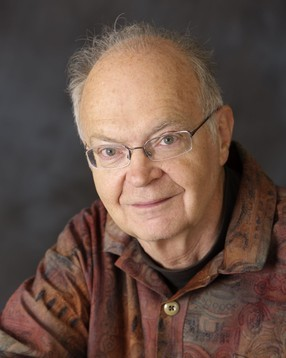
\includegraphics[width=.8\columnwidth]{support/images/Knuth.jpg}
    \end{column}
  \end{columns}
  \note{\emph{这一部分背景介绍大家可以了解一下,暂时跳过。}
  \LaTeX{} 这个词由两个部分组成,\hologo{La} 和 \TeX{}。那我们首先了解一下 \TeX{} 是什么。
  \TeX{} 是由斯坦福大学的教授高德纳于 1977 年开始开发的排版引擎,它已经有三十多年的历史了,
  目前仍在更新,版本号(3.141592653)将会趋近于 $\pi$ 的取值,高德纳最近还在给 \textsl{TUGBoat} 写稿子
  \link{https://tug.org/TUGboat/tb42-1/tb130knuth-tuneup21.pdf},
  关于 \TeX{} 今年又做了哪些改进。}
\end{frame}

\begin{frame}
  \frametitle{\LaTeX{}}
  \begin{columns}[c]
    \begin{column}{0.7\textwidth}
      \begin{center}
        \rmfamily\Huge
        \highlight[structure]{\LaTeX{}}
      \end{center}
      \begin{center}
        \parbox{0.75\textwidth}{
          \LaTeX{} 是最早在 1985 年由现就职于微软的 Leslie Lamport 开发的一种 \TeX{} \textbf{格式}\footnotemark,使用一些列宏和扩展宏包来简化 \TeX{} 的使用。现在由 \LaTeX{} Project 的成员维护。现在广泛使用的版本是 \LaTeXe{},最新的版本为 \LaTeX3(2020 年 10 月后默认内置)。
        }
      \end{center}
    \end{column}
    \begin{column}{0.3\textwidth}
      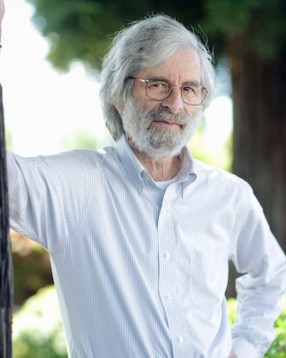
\includegraphics[width=.8\columnwidth]{support/images/Lamport.jpg}
    \end{column}
  \end{columns}
  \footnotetext{\hologo{ConTeXt} 也是一种 \TeX{} 格式 \link{https://www.contextgarden.net/}。}
  \note{\emph{这一部分的背景介绍大家可以了解一下,暂时跳过。}
  \LaTeX{} 是最早由现就职于微软的 Leslie Lamport 开发的一种 \TeX{} 格式(与其对标的是
  \hologo{ConTeXt}\link{https://www.contextgarden.net/}),主要也是为了简化 \TeX{} 的使用。
  现在主要由 \LaTeX{} 开发组维护,现在广泛使用的版本是 \LaTeXe{},最新的版本为 \LaTeX3,
  在 2020 年 10 月后默认内置,所以要尽可能使用较新的发行版,以充分发挥其功能。}
\end{frame}

\begin{frame}
  \frametitle{程序}
  \begin{columns}[c]
    \begin{column}{0.7\textwidth}
      \begin{center}
        \rmfamily\Huge
        \highlight[structure]{\hologo{pdfLaTeX}}
      \end{center}
      \begin{center}
        \parbox{0.7\textwidth}{
          \hologo{pdfLaTeX} 是为了编译一个 \LaTeX{} 文档而运行的程序。实际上底层在运行一个叫 \hologo{pdfTeX} 的引擎,并预装了对应的 \LaTeX{} \textbf{格式}。为了利用临时文件,可能就需要多次运行程序。
        }
      \end{center}
    \end{column}
    \begin{column}{0.3\textwidth}
      \begin{block}{}
        \ttfamily\small
        > \highlight{pdflatex} main.tex\\
        This is pdfTeX, Version 3.141592653-
        2.6-1.40.23 (MiKTeX 21.10)\\
        entering extended mode\\
        \highlight{LaTeX2e} <2021-11-15>\\
        \highlight{L3} programming layer <2021-11-22>
      \end{block}
    \end{column}
  \end{columns}
  \note{\hologo{pdfLaTeX} 是为了编译一个 \LaTeX{} 文档而运行的程序。}
\end{frame}

\begin{frame}
  \frametitle{引擎}
  \begin{columns}[c]
    \begin{column}{0.7\textwidth}
      \begin{center}
        \rmfamily\Huge
        \highlight[structure!70]{pdf}\hologo{La}\highlight[structure!70]{\TeX{}}
      \end{center}
      \begin{center}
        \parbox{0.7\textwidth}{
          pdf\TeX{} 是编译 \TeX{} 文档(以 \texttt{.tex} 结尾)的\textbf{引擎}---可以理解 \TeX{} 指令的\textbf{程序}。
        }
      \end{center}
    \end{column}
    \begin{column}{0.3\textwidth}
      \begin{block}{}
        \ttfamily\small
        > pdflatex main.tex\\
        This is \highlight[structure!70]{pdfTeX}, Version 3.141592653-
        2.6-1.40.23 (MiKTeX 21.10)
        entering extended mode\\
        LaTeX2e <2021-11-15>\\
        L3 programming layer <2021-11-22>
      \end{block}
    \end{column}
  \end{columns}
  \note{实际上底层在运行一个叫 \hologo{pdfTeX} 的引擎,并预装了对应的 \LaTeX{} 格式。}
\end{frame}

\begin{frame}[label={frame:engine}]
  \frametitle{Unicode 引擎}
  \begin{table}
    \caption{主流 \hologo{(La)TeX} 程序
    \footnote{(u)p\TeX{} 是日语最常用的引擎,生成 \texttt{.dvi},支持 Unicode。}\footnote{Ap\TeX{} \link{https://github.com/clerkma/ptex-ng} 具有底层 CJK 支持,内联 Ruby,Color Emoji。}}
    \footnotesize
    \begin{stampbox}
      \begin{tabular}{c>{\raggedright}*{3}{p{3.5cm}}}
        \alert{引擎}     & \hologo{pdfTeX}   & \hologo{XeTeX}   & \hologo{LuaTeX}   \\
        \alert{程序}     & \hologo{pdfLaTeX} & \hologo{XeLaTeX} & \hologo{LuaLaTeX} \\
        \alert{特点}     & 直接生成 PDF,支持 micro-typography  & 支持 Unicode、OpenType 与复杂文字编排 (CTL) & 支持 Unicode,内联 Lua,支持 OpenType \\
      \end{tabular}
    \end{stampbox}
  \end{table}

  \begin{center}
    \parbox{.9\textwidth}{
      \hologo{pdfLaTeX} 不支持 Unicode。为了排版中文,大部分情况下 \faApple{}\,\faLinux{} 应当使用 \hologo{XeLaTeX},而 \hologo{LuaLaTeX} 速度相对较慢。\faWindows{} 可以在一些情况下使用 \hologo{pdfLaTeX}。
    }
  \end{center}
  \note{当然为了排版中文,已经不再推荐使用 \hologo{pdfLaTeX} 了,应该使用 
  \hologo{XeLaTeX} 或者 \hologo{LuaLaTeX},当然后者的速度还是相对较慢,
  它们支持 Unicode 编码,并可以使用 OpenType 字体的全部功能。
  当然 \faWindows{} 平台下在某些追求速度的情况下,
  还是可以试着使用 \hologo{pdfLaTeX} 的。
  
  \hologo{LuaLaTeX} 理想情况下不慢,但是使用一些宏包后会破坏理想状态,
  也会因配置产生不同的结果,不同的操作系统在 I/O 速度上的不同也会导致不同的时间。

  \hologo{pdfLaTeX} 也支持,只不过需要先生成 tfm \TeX{} 字体度量文件,后续使用 \TeX{} 
  自身的配置方法,只能使用 7 比特或 8 比特字体。}
\end{frame}

% \begin{frame}
%   \paragraph{\hologo{pdfLaTeX}} \TeX{} 和 \LaTeX{} 被广泛使用之前,它们只需内置支持欧洲语言即可。在 Unicode 出现之前,\LaTeX{} 提供了许多种\textbf{文件编码}来允许很多语言的文字以原生的方式输入,\hologo{pdfLaTeX} 也只需要使用 8 位文件编码和 8 位字体。
% \end{frame}

\section{跑起来}
\begin{frame}
  \frametitle{发行版}
  \begin{table}
    \caption{\hologo{TeX} 发行版}
    \footnotesize
    \begin{stampbox}
      \begin{tabular}{c>{\raggedright}*{3}{p{3.2cm}}}
        \alert{发行版}     & \hologo{MiKTeX} \link{https://mirrors.sjtug.sjtu.edu.cn/ctan/systems/win32/miktex/setup/windows-x64/}   & \TeX{} Live \link{https://mirrors.sjtug.sjtu.edu.cn/ctan/systems/texlive/Images/}   & Mac\TeX{} \link{https://mirrors.sjtug.sjtu.edu.cn/ctan/systems/mac/mactex/}  \\[2pt]
        \alert{特点}      &  只安装必要文件,依赖用时更新  &  所有平台均可使用,每年发布一次 & Mac 系统专用,对 \TeX{} Live 的进一步打包 \\
        \alert{推荐平台}  & \faWindows  & \faLinux &  \faApple \\
      \end{tabular}
    \end{stampbox}
  \end{table}
  \begin{center}
    \parbox{.9\textwidth}{
      要让 \LaTeX{} 跑起来,核心就是要有一套 \TeX{} 发行版,来获取让 \LaTeX{} 工作所需的一组程序和文件。参考《一份简短的关于 \LaTeX{} 安装的介绍》\link{https://mirrors.sjtug.sjtu.edu.cn/ctan/info/install-latex-guide-zh-cn/install-latex-guide-zh-cn.pdf} 安装想使用的发行版。推荐使用发行版的最新版本\footnote{老版本 Linux 系统的包管理器自带 \TeX{} Live 发行版可能不是最新的 \link{https://repology.org/project/texlive/versions},尽量使用镜像安装,并手动将相关环境变量添加到路径 \link{https://www.tug.org/texlive/doc/texlive-zh-cn/texlive-zh-cn.pdf}。},并使用国内镜像。
    }
  \end{center}
  \note{要让 \LaTeX{} 跑起来,核心就是要有一套 \TeX{} 发行版,来获取让 
  \LaTeX{} 工作所需的一组程序和文件。参考《一份简短的关于 \LaTeX{} 安装的介绍》
  安装想使用的发行版,里面介绍了 \faWindows{}, \faApple{}, \faLinux{}, WSL 等系统上
  \TeX{} Live 的安装,非常全面,一步一步做就可以成功安装。目前最新的 \TeX{} Live 版本为
  2022,\SJTUThesis{} 用户不应当安装 \TeX{} Live 2020 以下的版本(后面会讲)。
  
  事实上,我认为这几个发行版各有操作系统偏好,虽然前两者是跨平台的。

  \hologo{MiKTeX} 对 Windows 用户较为友好,安装简单,占用空间不大,安装时间短,
  而且有完整的安装与卸载程序。可以给大家看一下 \hologo{MiKTeX} Console 的情况。

  \TeX{} Live 更符合 Linux 的更新传统。老版本 Linux 系统的包管理器自带 \TeX{} Live
  发行版可能不是最新的(到时间也会锁定依赖库的版本),尽量使用镜像安装(当然也推荐使用最新的
  Linux 发行版,这样它的版本也就一直是最新的),并手动将相关环境变量添加到路径。

  Mac\TeX{} 发行版有 pkg 安装包封装,并且附带了 \TeX{}Shop 基本编辑软件,更加适合 Mac OS。
  我用下来的话,感觉除了 \TeX{} Live Utility 外都有点过时了。}
\end{frame}

\begin{frame}[plain]
  \hbox to \textwidth{
    \hfil
    \vbox to 3cm{
      \hbox{
        \resizebox{3cm}{!}{
\includegraphics{support/examples/pics/sjtug}}
      }
    }
    \hfil
    \vbox to 3cm{
      \vfill
      \hbox{\Large\bfseries\color{structure} 稳定、快速、现代的镜像服务。}
      \vskip2pt
      \hbox{托管于华东教育网骨干节点上海交通大学。}
      \vfill
    }
    \hskip20pt
    \hfil
  }

  \begin{center}
    \parbox{0.8\textwidth}{
      推荐使用 SJTUG 软件镜像服务 \link{https://mirror.sjtu.edu.cn/},离得近,下得快。
      
      \begin{description}
        \footnotesize
        \item[\TeX{} Live]  {\ttfamily tlmgr option repository https://mirrors.sjtug.sjtu.edu.cn/CTAN/systems/texlive/tlnet}
        \item[\hologo{MiKTeX}] 在 \hologo{MiKTeX} Console 中设置镜像源为 \url{https://mirrors.sjtug.sjtu.edu.cn}
        \item[\faTelegram] 可以在 SJTUG 镜像站通知频道 \link{https://t.me/sjtug_mirrors_news} 获得更多信息,加入关联群组参与讨论。
      \end{description}
    }
  \end{center}
  \note{说到镜像,像后两者的安装包都很大(4GB 左右),由于一些原因,不采用镜像的话不知道要下到什么时候,对下载速度的要求高;
  而 \hologo{MiKTeX} 需要随时更新,宏包大小颗粒度大,对延迟的要求高。
  那么采用 SJTUG 镜像源将同时解决这两个问题,位于图信大楼的机房,凭借校内的高速网络,稳定快速下载,
  现在由 LightQuantum 维护的镜像站欢迎大家的使用,主页上还有更多的其他镜像可供使用,加入 Telegram 群组参与讨论。}
\end{frame}

\begin{frame}
  \frametitle{编辑器}
  \begin{table}
    \caption{开源编辑器推荐}
    \footnotesize
    \begin{stampbox}
      \begin{tabular}{c>{\raggedright}*{3}{p{3.5cm}}}
        \alert{编辑器}     & \begin{tabular}{c}Visual Studio Code \link{https://code.visualstudio.com}\\ \LaTeX{} Workshop\end{tabular}  & \TeX{}studio \link{https://texstudio.org} & \TeX{}works \\[5pt]
        \alert{特点}      &  搭配 VS Code 使用非常方便,易扩展  & 可以使用大量的菜单选项输入代码块,用户友好 & 只提供基础的高亮与运行方法,发行版自带\footnote{Mac\TeX{} 打包的是 \TeX{}Shop 编辑器。} \\
      \end{tabular}
    \end{stampbox}
  \end{table}
  \begin{center}
    \parbox{.9\textwidth}{
      使用专为 \LaTeX{} 设计的编辑器将带来更多便利,因为它们往往会提供一键编译、内置 PDF 阅读器以及语法高亮等功能。几乎所有现代的 \LaTeX{} 编辑器都提供 Sync\TeX{} 这一强大的功能,以在 PDF 和代码间对应跳转。
    }
  \end{center}
  \note{编辑器的种类很多,我无法一一列举,但是对编写 \TeX{} 常用的开源编辑器我推荐这三个。
  其中 \TeX{}studio 的安装包可能下得有点慢。这里我对这些编辑器都演示一下,初学者我更推荐使用
  \TeX{} studio 编辑器,如果平时就码很多代码的话,我更推荐使用 VS Code 加插件这种方式。
  
  使用专为 \LaTeX{} 设计的编辑器将带来更多便利,因为它们往往会提供一键编译、内置 PDF 阅读器
  以及语法高亮等功能。几乎所有现代的 \LaTeX{} 编辑器都提供 Sync\TeX{} 这一强大的功能
  (VS Code 的方法是 Ctrl + 某处,Overleaf 的方法是直接双击),以在 PDF 和代码间对应跳转。
  当然如果你不喜欢使用这种 GUI 编辑器,\TeX{} 文档本身就是纯文本,对 Vim, Emacs 等终端用户
  也很友好。}
\end{frame}

\begin{frame}
  \frametitle{在线平台}
  \begin{table}
    \caption{在线协作平台推荐}
    \footnotesize
    \begin{stampbox}
      \begin{tabular}{c>{\raggedright}*{2}{p{4cm}}}
        \alert{在线平台}     & Overleaf \link{https://www.overleaf.com/}  & 交大 \LaTeX{} 助手 \link{https://latex.sjtu.edu.cn/} \\[2pt]
        \alert{特点}      & 最流行的在线平台,提供大量的模板,但国内访问慢 & 校内平台,隐私保护有保障,共享项目限制少 \\
      \end{tabular}
    \end{stampbox}
  \end{table}
  \begin{center}
    \parbox{.9\textwidth}{
      在线平台允许你直接在网页中编辑文档,无需本地安装即可在后台运行 \LaTeX{},并显示生成的 PDF。可以参照 Overleaf 官方文档学习如何使用在线平台 \link{https://www.overleaf.com/learn}。
    }
  \end{center}
  \note{当然使用在线平台省去了安装发行版的麻烦,这里列出两种在线写作平台。

  如果有数据合规需求的话,可以考虑使用由网络信息中心维护的交大 \LaTeX{} 助手,最近更新了 \TeX{} Live 2022,还是很不错的。

  当然国内还有 \TeX{} Page \link{https://www.texpage.com/},Slagger \link{https://www.slager.cn/} 等。
  一般来讲,这种平台使用的都是 Linux 操作系统,所以在排版中文的时候考虑将编译引擎更改为 \hologo{XeLaTeX},
  学习如何使用在线平台参见 Overleaf 的官方文档 \link{https://www.overleaf.com/learn}。}
\end{frame}

\section{基本结构}
\begin{frame}[fragile]%
  \frametitle{文档部件}
  \begin{columns}[c]
    \begin{column}{0.4\textwidth}
      \only<1>{
        \cmd{documentclass} 命令加载了\textbf{文档类}。\cls{article} 是由 \LaTeX{} 提供的用于排版短文档的基本文档类。
        \begin{description}
          \footnotesize
          \item[\cls{article}] 不包含章的短文档
          \item[\cls{report}] 含有章的单面印刷文档
          \item[\cls{book}] 含有章的双面印刷文档
          \item[\cls{beamer}] 幻灯片
        \end{description}
      }

      \only<2>{
        \env{document} 环境用于指示文档主体的范围。\LaTeX{} 还有其他的使用 \cmd{begin} 和 \cmd{end} 的搭配,我们称这些为\textbf{环境}。它们将用来设定局部格式命令\footnotemark。
      }

      \only<3>{
        \includepdflarge{support/examples/enminimal.pdf}
      }
    \end{column}
    \begin{column}{0.6\textwidth}
      \begin{codeblock}[]{排版英文最简示例}
|\highlightline<1>|\documentclass{article}
|\highlightline<2>|\begin{document}
|\highlightline<3>|  Together for a Shared Future
|\highlightline<2>|\end{document}
      \end{codeblock}
    \end{column}
  \end{columns}

  \only<2>{\footnotetext{环境实际上是一个组,只不过通过语义化的形式预装了对应的格式命令。普通的组可以直接使用一对大括号之间的内容 \{$\cdots$\} 表示。}}
\end{frame}

\section{扩展}
\begin{frame}[fragile]%
  \frametitle{中文排版}
  \begin{columns}[c]
    \begin{column}{0.4\textwidth}

      \only<1>{
        \cmd{usepackage} 用于使用宏包以向 \LaTeX{} 添加或修改功能,需要在\textbf{导言区}调用。
        这里使用 \pkg{ctex} 宏集以获得中文支持。其调用底层因不同的引擎而不同。
        \begin{center}
          \footnotesize
          \begin{tabular}{c*{3}{c}}
            \alert{引擎}     & \hologo{pdfTeX}   & \hologo{XeTeX}   & \hologo{LuaTeX}   \\
            \alert{程序}     & \hologo{pdfLaTeX} & \hologo{XeLaTeX} & \hologo{LuaLaTeX} \\
            \alert{宏包}     & CJK\footnotemark & xeCJK & luatexja \\
            \alert{封装}     & \multicolumn{3}{c}{ctex} \\
          \end{tabular}
        \end{center}
        \vspace{-1cm}
      }

      \only<2>{
        \CTeX{} 建议对于之前提到的常规文档类,最佳实践是使用该宏集提供的四种中文文档类,以对特定类型提供额外的中文排版适配。
        \begin{center}
          \footnotesize
          \begin{tabular}{cc}
            \cls{ctexart} & \cls{ctexrep} \\
            \cls{ctexbook} & \cls{ctexbeamer} \\
          \end{tabular}
        \end{center}
      }

      \only<3>{
        \includepdflarge{support/examples/cnminimal.pdf}
      }

      \only<4>{
        大部分情况下,你都不应当在 \LaTeX{} 中强制断行:你几乎只是想另起一段,或者是想在段落之间添加空行(使用 \pkg{parskip} 宏包就可实现)。
        只有\alert{很少的}情况下你需要使用 \textbackslash{}\textbackslash{} 来另起一行而不另起一段(强制断行仍在同一段)。
      }
    \end{column}
    \begin{column}{0.6\textwidth}
      \begin{codeblock}[]{排版中文\only<2->{最佳实践}}
|\highlightline<2>|\documentclass{|\only<1>{article}\only<2->{ctexart}|}
|\only<1>{\highlightline\textbackslash{}usepackage\{ctex\}\hfill\color{structure}\% 导言区}|
\begin{document}
|\highlightline<3>|    一起向未来
|\highlightline<4>|
  Together for a Shared Future
\end{document}
      \end{codeblock}
    \end{column}
  \end{columns}
  \only<1>{\footnotetext{ctex 在 \faApple\,\faLinux{} 上已经不可以使用 \hologo{pdfLaTeX} 编译,以及在 \faWindows{} 上使用该引擎也会变更自动间距调整等功能的默认行为。}}
\end{frame}

\section{设定格式}
\begin{frame}[fragile]%
  \frametitle{字体样式}
  \begin{columns}
    \begin{column}{0.4\textwidth}
      \only<1>{
        \includepdflarge{support/examples/fontstyle.pdf}
      }

      \only<2>{
        可以使用显式样式设定命令对小段做加粗、斜体、等宽等等的处理。
        \begin{center}
          \footnotesize
          \begin{tabular}{rl}
            \cmd{textrm} & \textrm{衬线} \\
            \cmd{textbf} & \textbf{加粗} \\
            \cmd{textit} & \kaishu 斜体 \\
            \cmd{texttt} & \texttt{等宽} \\
            \cmd{textsf} & \textsf{无衬线} \\
            \cmd{textsc} & \textsc{Small Caps} \\
            \cmd{textsl} & \textsl{Slanted} \\
          \end{tabular}
        \end{center}
      }

      \only<3>{
        与 Word 不同的是,\LaTeX{} 一般情况下并不需要使用上面的显式命令,而是采用逻辑标记的方法,
        比如 \cmd{emph} 可以强调文字,以及下面将要提到的目次命令(第 \ref{sectioning} 页)。
        这样可以统一管理格式。
      }
    \end{column}
    \begin{column}{0.6\textwidth}
      \begin{codeblock}[]{样式}
\documentclass{ctexart}
\begin{document}
|\highlightline<2>|  \textbf{|\phantom{}|一起向未来}

|\highlightline<3>|  \emph{Together for a Shared Future}
\end{document}
      \end{codeblock}
    \end{column}
  \end{columns}
\end{frame}

\begin{frame}[fragile]%
  \frametitle{\only<1-2>{字体大小}\only<3>{字体样式}}
  \begin{columns}
    \begin{column}{0.4\textwidth}
      \only<1>{
        \includepdflarge{support/examples/fontsize.pdf}
      }

      \only<2>{
        同样地,你也可以显式地设定字体大小,但是这种命令会更改行文设置,所以需要使用一个组来限定作用范围\footnotemark。
        \begin{center}
          \footnotesize
          \begin{tabular}{rl}
            \cmd{tiny} & \tiny 极小 \\
            \cmd{scriptsize} & \scriptsize 角标大小  \\
            \cmd{footnotesize} & \footnotesize 脚注大小 \\
            \cmd{small} & \small 小 \\
            \cmd{normalsize} & \normalsize 正常大小 \\
            \cmd{large} & \large 大 \\
            \cmd{huge} & \Huge 巨大 \\
          \end{tabular}
        \end{center}
      }

      \only<3>{
        也可以使用字体样式对应的更改字体设置的命令,这对于大段文段的设置而言也是很方便的。
        \begin{center}
          \footnotesize
          \begin{tabular}{ll}
            \cmd{textrm} & \cmd{rmfamily}\\
            \cmd{texttt} & \cmd{ttfamily}\\
            \cmd{textsf} & \cmd{sffamily}\\
            \cmd{textbf} & \cmd{bfseries}\\
            \cmd{textit} & \cmd{itshape}\\
            \cmd{textsc} & \cmd{scshape}\\
            \cmd{textsl} & \cmd{slshape}\\
          \end{tabular}
        \end{center}
      }
    \end{column}
    \begin{column}{0.6\textwidth}
      \begin{codeblock}[]{大小}
\documentclass{ctexart}
\begin{document}
|\highlightline<2>|  {\bfseries\Large 一起向未来\par}
|\highlightline<3>|  {\itshape Together for a Shared Future}
\end{document}
      \end{codeblock}
    \end{column}
  \end{columns}

  \only<2>{\footnotetext{注意最后显式地使用 \cmd{par} 在改回大小前结束该段,否则会导致下一行的行间距异常!}}
\end{frame}

\section{逻辑结构}
\begin{frame}[fragile]
  \frametitle{列表}
  \begin{columns}
    \begin{column}{0.35\textwidth}
      \begin{codeblock}[]{无序列表}
\documentclass{ctexart}
\begin{document}
|\highlightline|  \begin{itemize}
    \item 第一项
    \item 第二项
    \item 第三项
|\highlightline|  \end{itemize}
\end{document}
      \end{codeblock}
    \end{column}
    \begin{column}{0.35\textwidth}
      \begin{codeblock}[]{有序列表}
\documentclass{ctexart}
\begin{document}
|\highlightline|  \begin{enumerate}
    \item 第一项
    \item 第二项
    \item 第三项
|\highlightline|  \end{enumerate}
\end{document}
      \end{codeblock}
    \end{column}
    \begin{column}{0.35\textwidth}
      \begin{codeblock}[]{描述列表}
\documentclass{ctexart}
\begin{document}
|\highlightline|  \begin{description}
    \item[|\phantom{}|第一] 文本
    \item[|\phantom{}|第二] 文本
    \item[|\phantom{}|第三] 文本  
|\highlightline|  \end{description}
\end{document}
      \end{codeblock}
    \end{column}
  \end{columns}
  \note{接下来我们概览一下三种列表:无序列表、有序列表、描述列表。这些列表可以相互嵌套,但最多嵌套四层。}
\end{frame}

%更深的列表技巧,定理环境等

\begin{frame}
  \frametitle{列表}
  \begin{columns}
    \begin{column}{0.35\textwidth}
      \includepdflarge{support/examples/unordered.pdf}
    \end{column}
    \begin{column}{0.35\textwidth}
      \includepdflarge{support/examples/ordered.pdf}
    \end{column}
    \begin{column}{0.35\textwidth}
      \includepdflarge{support/examples/description.pdf}
    \end{column}
  \end{columns}
\end{frame}

\begin{frame}[fragile,label=sectioning]%
  \frametitle{目次结构}
  \begin{columns}
    \begin{column}{0.4\textwidth}
      \LaTeX{} 可以使用目次命令将文档划分层级\footnotemark,并自动设定对应字体样式和大小。
      \begin{center}
        \footnotesize
        \begin{tabular}{rll}
          命令 & 含义 & 层次 \\
          \cmd{chapter} & 章\footnotemark & \sout{0} \\
          \cmd{section} & 节 & 1 \\
          \cmd{subsection} & 小节 & 2 \\
          \cmd{subsubsection} & 小小节 & 3 \\
        \end{tabular}
      \end{center}
    \end{column}
    \begin{column}{0.6\textwidth}
      \begin{codeblock}[]{目次}
\documentclass{ctexart}
\begin{document}
|\highlightline|  \section{|\phantom{}|概念}
|\highlightline|  \subsection{\LaTeX{}}
  \LaTeX{} 是一个用以排版高质量作品的文档准备系统。
\end{document}
      \end{codeblock}
    \end{column}
  \end{columns}
  \footnotetext{章这一级只在 \cls{report} 和 \cls{book} 文档类(包括对应的中文文档类)有定义。还有不常用的 \cmd{part} (0@\cls{article}/-1@\cls{report}\&\cls{book}\&\cls{beamer}) 以及更低层次的 \cmd{paragraph} (4) 与 \cmd{subparagraph} (5)。 }
  \note{而知道层次,对我们下面生成目录有帮助。}
\end{frame}

\begin{frame}[fragile]%
  \frametitle{组织文档}
  \begin{columns}
    \begin{column}{0.4\textwidth}

      \only<1>{
        \cmd{tableofcontents} 用来生成对于目次命令的目录。如果你想设定显示到哪个层级,在这个命令前使用 \cmd{setcounter\{tocdepth\}\{层次\}}

        如果你想在目录中使用更短的标题:

            \cmd{section[短标题]\{长标题\}}

        如果你想让本目次的标题不显示在目录中:

            \cmd{section*\{目录没这个标题\}}
      }

      \only<2>{
        对于大型文档而言,使用多个文件管理源文件通常是更方便的。而 \cmd{include} 和 \cmd{input} 都以相对路径的方式插入其他 \TeX{} 文档。
        区别在于,\cmd{include} 命令会从新页开始并做一些内部调整,这基本上只对 \pkg{chapter} 这一级有用。而 \cmd{input} 会原样插入源代码。
      }

      \only<3>{
        但是 \cmd{include} 插入的文档可以使用 \cmd{includeonly} 管理当前要排印哪一部分的内容,利用所有章节辅助文件的同时,减少编译时间并专注于该部分的内容。
      }
    \end{column}
    \begin{column}{0.6\textwidth}
      \begin{codeblock}[]{主文档}
\documentclass{ctexrep}
|\highlightline<3>|\includeonly{learnlatex,sjtuthesis}
\begin{document}
|\highlightline<1>|  \tableofcontents
|\only<2-3>{\highlightline}|  % !TeX root = ../../latex-talk.tex

\part{学习 \LaTeX{}}
% FIXME: footnote fault numbering
% FIXME: section pop up in navigation in advance

\begin{frame}
  \frametitle{本部分主要参考}
  \begin{bibliolist}{00}
    \onlineitem 陈晟祺~等.
    \newblock 如何使用 \LaTeX\ 排版论文[EB/OL].
    \newblock 2021. \url{https://github.com/tuna/thulib-latex-talk}.

    \onlineitem 曾祥东.
    \newblock 现代 \LaTeX\ 入门讲座[EB/OL].
    \newblock 2022. \url{https://github.com/stone-zeng/latex-talk}.

    \onlineitem \LaTeX\ Project.
    \CTeX\ 开发小组~译.
    \newblock learnlatex.org[EB/OL].
    \newblock 2022. \url{https://github.com/CTeX-org/learnlatex.github.io}.
  
    \onlineitem \textsc{Oetiker T}, \textsc{Partl H}, \textsc{Hyna I}, \textsc{Schlegl E}.
    \CTeX\ 开发小组~译.
    \newblock 一份(不太)简短的 \LaTeXe{} 介绍:或 111 分钟了解 \LaTeXe{}[EB/OL]. \newblock\newblock 2021.
    \url{https://ctan.org/pkg/lshort-zh-cn}.
  \end{bibliolist}

  \note{推荐大家去阅读这些入门材料。}
\end{frame}

\begin{frame}[plain]
  \vfil
  \begin{center}
    \href{https://learnlatex.org}{
      \rmfamily
      Learn\,\lower1ex\hbox{\Huge\LaTeX{}}.org
    }
  \end{center}
  \vfil
  \begin{center}
    \parbox{0.75\linewidth}{
      Learn\LaTeX{}.org 提供了解 \LaTeX{} 的 16 篇简短的教程,并包含了一些可以在线运行的示例,可以通过亲自动手查看实验效果。本部分主要参考由 \CTeX{}-org 提供的中文翻译版本 \link{https://github.com/CTeX-org/learnlatex.github.io/tree/zh-Hans/zh-Hans/}。
    }
  \end{center}
  \vfil
  \note{这一部分主要参考了 Learn\LaTeX{}.org 的系列教程,内容简洁,适合入门,符合
  教育学观念 \link{https://www.tug.org/TUGboat/tb41-2/tb128reviews-learnlatex.pdf},
  并参考由 \CTeX{}-org 提供的中文翻译版本
  \link{https://github.com/CTeX-org/learnlatex.github.io/tree/zh-Hans/zh-Hans/}。
  如果你认为下面一个小时的入门教程没有讲得非常细致的话,
  欢迎直接阅读这个网站的全文。}
\end{frame}

\begin{shadedsection}

\section{是什么}
\begin{frame}
  \frametitle{\TeX{}}
  \begin{columns}[c]
    \begin{column}{0.7\textwidth}
      \begin{center}
        \rmfamily\Huge
        \hologo{La}\highlight[structure!70]{\TeX{}}
      \end{center}
      \begin{center}
        \parbox{0.75\textwidth}{
          \TeX{} 是由斯坦福大学教授高德纳
          (Donald E.~Knuth)于 1977 年开始开发的排版引擎。目前仍在更新,最新版本号为 3.141592653 \link{https://tug.org/TUGboat/tb42-1/tb130knuth-tuneup21.pdf}。
        }
      \end{center}
    \end{column}
    \begin{column}{0.3\textwidth}
      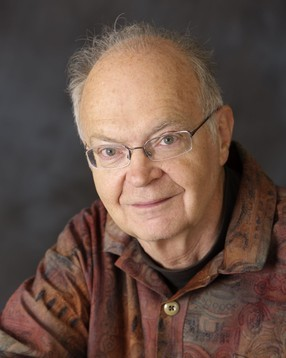
\includegraphics[width=.8\columnwidth]{support/images/Knuth.jpg}
    \end{column}
  \end{columns}
  \note{\emph{这一部分背景介绍大家可以了解一下,暂时跳过。}
  \LaTeX{} 这个词由两个部分组成,\hologo{La} 和 \TeX{}。那我们首先了解一下 \TeX{} 是什么。
  \TeX{} 是由斯坦福大学的教授高德纳于 1977 年开始开发的排版引擎,它已经有三十多年的历史了,
  目前仍在更新,版本号(3.141592653)将会趋近于 $\pi$ 的取值,高德纳最近还在给 \textsl{TUGBoat} 写稿子
  \link{https://tug.org/TUGboat/tb42-1/tb130knuth-tuneup21.pdf},
  关于 \TeX{} 今年又做了哪些改进。}
\end{frame}

\begin{frame}
  \frametitle{\LaTeX{}}
  \begin{columns}[c]
    \begin{column}{0.7\textwidth}
      \begin{center}
        \rmfamily\Huge
        \highlight[structure]{\LaTeX{}}
      \end{center}
      \begin{center}
        \parbox{0.75\textwidth}{
          \LaTeX{} 是最早在 1985 年由现就职于微软的 Leslie Lamport 开发的一种 \TeX{} \textbf{格式}\footnotemark,使用一些列宏和扩展宏包来简化 \TeX{} 的使用。现在由 \LaTeX{} Project 的成员维护。现在广泛使用的版本是 \LaTeXe{},最新的版本为 \LaTeX3(2020 年 10 月后默认内置)。
        }
      \end{center}
    \end{column}
    \begin{column}{0.3\textwidth}
      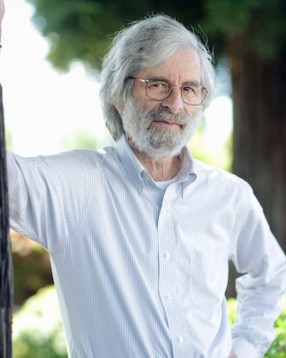
\includegraphics[width=.8\columnwidth]{support/images/Lamport.jpg}
    \end{column}
  \end{columns}
  \footnotetext{\hologo{ConTeXt} 也是一种 \TeX{} 格式 \link{https://www.contextgarden.net/}。}
  \note{\emph{这一部分的背景介绍大家可以了解一下,暂时跳过。}
  \LaTeX{} 是最早由现就职于微软的 Leslie Lamport 开发的一种 \TeX{} 格式(与其对标的是
  \hologo{ConTeXt}\link{https://www.contextgarden.net/}),主要也是为了简化 \TeX{} 的使用。
  现在主要由 \LaTeX{} 开发组维护,现在广泛使用的版本是 \LaTeXe{},最新的版本为 \LaTeX3,
  在 2020 年 10 月后默认内置,所以要尽可能使用较新的发行版,以充分发挥其功能。}
\end{frame}

\begin{frame}
  \frametitle{程序}
  \begin{columns}[c]
    \begin{column}{0.7\textwidth}
      \begin{center}
        \rmfamily\Huge
        \highlight[structure]{\hologo{pdfLaTeX}}
      \end{center}
      \begin{center}
        \parbox{0.7\textwidth}{
          \hologo{pdfLaTeX} 是为了编译一个 \LaTeX{} 文档而运行的程序。实际上底层在运行一个叫 \hologo{pdfTeX} 的引擎,并预装了对应的 \LaTeX{} \textbf{格式}。为了利用临时文件,可能就需要多次运行程序。
        }
      \end{center}
    \end{column}
    \begin{column}{0.3\textwidth}
      \begin{block}{}
        \ttfamily\small
        > \highlight{pdflatex} main.tex\\
        This is pdfTeX, Version 3.141592653-
        2.6-1.40.23 (MiKTeX 21.10)\\
        entering extended mode\\
        \highlight{LaTeX2e} <2021-11-15>\\
        \highlight{L3} programming layer <2021-11-22>
      \end{block}
    \end{column}
  \end{columns}
  \note{\hologo{pdfLaTeX} 是为了编译一个 \LaTeX{} 文档而运行的程序。}
\end{frame}

\begin{frame}
  \frametitle{引擎}
  \begin{columns}[c]
    \begin{column}{0.7\textwidth}
      \begin{center}
        \rmfamily\Huge
        \highlight[structure!70]{pdf}\hologo{La}\highlight[structure!70]{\TeX{}}
      \end{center}
      \begin{center}
        \parbox{0.7\textwidth}{
          pdf\TeX{} 是编译 \TeX{} 文档(以 \texttt{.tex} 结尾)的\textbf{引擎}---可以理解 \TeX{} 指令的\textbf{程序}。
        }
      \end{center}
    \end{column}
    \begin{column}{0.3\textwidth}
      \begin{block}{}
        \ttfamily\small
        > pdflatex main.tex\\
        This is \highlight[structure!70]{pdfTeX}, Version 3.141592653-
        2.6-1.40.23 (MiKTeX 21.10)
        entering extended mode\\
        LaTeX2e <2021-11-15>\\
        L3 programming layer <2021-11-22>
      \end{block}
    \end{column}
  \end{columns}
  \note{实际上底层在运行一个叫 \hologo{pdfTeX} 的引擎,并预装了对应的 \LaTeX{} 格式。}
\end{frame}

\begin{frame}[label={frame:engine}]
  \frametitle{Unicode 引擎}
  \begin{table}
    \caption{主流 \hologo{(La)TeX} 程序
    \footnote{(u)p\TeX{} 是日语最常用的引擎,生成 \texttt{.dvi},支持 Unicode。}\footnote{Ap\TeX{} \link{https://github.com/clerkma/ptex-ng} 具有底层 CJK 支持,内联 Ruby,Color Emoji。}}
    \footnotesize
    \begin{stampbox}
      \begin{tabular}{c>{\raggedright}*{3}{p{3.5cm}}}
        \alert{引擎}     & \hologo{pdfTeX}   & \hologo{XeTeX}   & \hologo{LuaTeX}   \\
        \alert{程序}     & \hologo{pdfLaTeX} & \hologo{XeLaTeX} & \hologo{LuaLaTeX} \\
        \alert{特点}     & 直接生成 PDF,支持 micro-typography  & 支持 Unicode、OpenType 与复杂文字编排 (CTL) & 支持 Unicode,内联 Lua,支持 OpenType \\
      \end{tabular}
    \end{stampbox}
  \end{table}

  \begin{center}
    \parbox{.9\textwidth}{
      \hologo{pdfLaTeX} 不支持 Unicode。为了排版中文,大部分情况下 \faApple{}\,\faLinux{} 应当使用 \hologo{XeLaTeX},而 \hologo{LuaLaTeX} 速度相对较慢。\faWindows{} 可以在一些情况下使用 \hologo{pdfLaTeX}。
    }
  \end{center}
  \note{当然为了排版中文,已经不再推荐使用 \hologo{pdfLaTeX} 了,应该使用 
  \hologo{XeLaTeX} 或者 \hologo{LuaLaTeX},当然后者的速度还是相对较慢,
  它们支持 Unicode 编码,并可以使用 OpenType 字体的全部功能。
  当然 \faWindows{} 平台下在某些追求速度的情况下,
  还是可以试着使用 \hologo{pdfLaTeX} 的。
  
  \hologo{LuaLaTeX} 理想情况下不慢,但是使用一些宏包后会破坏理想状态,
  也会因配置产生不同的结果,不同的操作系统在 I/O 速度上的不同也会导致不同的时间。

  \hologo{pdfLaTeX} 也支持,只不过需要先生成 tfm \TeX{} 字体度量文件,后续使用 \TeX{} 
  自身的配置方法,只能使用 7 比特或 8 比特字体。}
\end{frame}

% \begin{frame}
%   \paragraph{\hologo{pdfLaTeX}} \TeX{} 和 \LaTeX{} 被广泛使用之前,它们只需内置支持欧洲语言即可。在 Unicode 出现之前,\LaTeX{} 提供了许多种\textbf{文件编码}来允许很多语言的文字以原生的方式输入,\hologo{pdfLaTeX} 也只需要使用 8 位文件编码和 8 位字体。
% \end{frame}

\section{跑起来}
\begin{frame}
  \frametitle{发行版}
  \begin{table}
    \caption{\hologo{TeX} 发行版}
    \footnotesize
    \begin{stampbox}
      \begin{tabular}{c>{\raggedright}*{3}{p{3.2cm}}}
        \alert{发行版}     & \hologo{MiKTeX} \link{https://mirrors.sjtug.sjtu.edu.cn/ctan/systems/win32/miktex/setup/windows-x64/}   & \TeX{} Live \link{https://mirrors.sjtug.sjtu.edu.cn/ctan/systems/texlive/Images/}   & Mac\TeX{} \link{https://mirrors.sjtug.sjtu.edu.cn/ctan/systems/mac/mactex/}  \\[2pt]
        \alert{特点}      &  只安装必要文件,依赖用时更新  &  所有平台均可使用,每年发布一次 & Mac 系统专用,对 \TeX{} Live 的进一步打包 \\
        \alert{推荐平台}  & \faWindows  & \faLinux &  \faApple \\
      \end{tabular}
    \end{stampbox}
  \end{table}
  \begin{center}
    \parbox{.9\textwidth}{
      要让 \LaTeX{} 跑起来,核心就是要有一套 \TeX{} 发行版,来获取让 \LaTeX{} 工作所需的一组程序和文件。参考《一份简短的关于 \LaTeX{} 安装的介绍》\link{https://mirrors.sjtug.sjtu.edu.cn/ctan/info/install-latex-guide-zh-cn/install-latex-guide-zh-cn.pdf} 安装想使用的发行版。推荐使用发行版的最新版本\footnote{老版本 Linux 系统的包管理器自带 \TeX{} Live 发行版可能不是最新的 \link{https://repology.org/project/texlive/versions},尽量使用镜像安装,并手动将相关环境变量添加到路径 \link{https://www.tug.org/texlive/doc/texlive-zh-cn/texlive-zh-cn.pdf}。},并使用国内镜像。
    }
  \end{center}
  \note{要让 \LaTeX{} 跑起来,核心就是要有一套 \TeX{} 发行版,来获取让 
  \LaTeX{} 工作所需的一组程序和文件。参考《一份简短的关于 \LaTeX{} 安装的介绍》
  安装想使用的发行版,里面介绍了 \faWindows{}, \faApple{}, \faLinux{}, WSL 等系统上
  \TeX{} Live 的安装,非常全面,一步一步做就可以成功安装。目前最新的 \TeX{} Live 版本为
  2022,\SJTUThesis{} 用户不应当安装 \TeX{} Live 2020 以下的版本(后面会讲)。
  
  事实上,我认为这几个发行版各有操作系统偏好,虽然前两者是跨平台的。

  \hologo{MiKTeX} 对 Windows 用户较为友好,安装简单,占用空间不大,安装时间短,
  而且有完整的安装与卸载程序。可以给大家看一下 \hologo{MiKTeX} Console 的情况。

  \TeX{} Live 更符合 Linux 的更新传统。老版本 Linux 系统的包管理器自带 \TeX{} Live
  发行版可能不是最新的(到时间也会锁定依赖库的版本),尽量使用镜像安装(当然也推荐使用最新的
  Linux 发行版,这样它的版本也就一直是最新的),并手动将相关环境变量添加到路径。

  Mac\TeX{} 发行版有 pkg 安装包封装,并且附带了 \TeX{}Shop 基本编辑软件,更加适合 Mac OS。
  我用下来的话,感觉除了 \TeX{} Live Utility 外都有点过时了。}
\end{frame}

\begin{frame}[plain]
  \hbox to \textwidth{
    \hfil
    \vbox to 3cm{
      \hbox{
        \resizebox{3cm}{!}{
\includegraphics{support/examples/pics/sjtug}}
      }
    }
    \hfil
    \vbox to 3cm{
      \vfill
      \hbox{\Large\bfseries\color{structure} 稳定、快速、现代的镜像服务。}
      \vskip2pt
      \hbox{托管于华东教育网骨干节点上海交通大学。}
      \vfill
    }
    \hskip20pt
    \hfil
  }

  \begin{center}
    \parbox{0.8\textwidth}{
      推荐使用 SJTUG 软件镜像服务 \link{https://mirror.sjtu.edu.cn/},离得近,下得快。
      
      \begin{description}
        \footnotesize
        \item[\TeX{} Live]  {\ttfamily tlmgr option repository https://mirrors.sjtug.sjtu.edu.cn/CTAN/systems/texlive/tlnet}
        \item[\hologo{MiKTeX}] 在 \hologo{MiKTeX} Console 中设置镜像源为 \url{https://mirrors.sjtug.sjtu.edu.cn}
        \item[\faTelegram] 可以在 SJTUG 镜像站通知频道 \link{https://t.me/sjtug_mirrors_news} 获得更多信息,加入关联群组参与讨论。
      \end{description}
    }
  \end{center}
  \note{说到镜像,像后两者的安装包都很大(4GB 左右),由于一些原因,不采用镜像的话不知道要下到什么时候,对下载速度的要求高;
  而 \hologo{MiKTeX} 需要随时更新,宏包大小颗粒度大,对延迟的要求高。
  那么采用 SJTUG 镜像源将同时解决这两个问题,位于图信大楼的机房,凭借校内的高速网络,稳定快速下载,
  现在由 LightQuantum 维护的镜像站欢迎大家的使用,主页上还有更多的其他镜像可供使用,加入 Telegram 群组参与讨论。}
\end{frame}

\begin{frame}
  \frametitle{编辑器}
  \begin{table}
    \caption{开源编辑器推荐}
    \footnotesize
    \begin{stampbox}
      \begin{tabular}{c>{\raggedright}*{3}{p{3.5cm}}}
        \alert{编辑器}     & \begin{tabular}{c}Visual Studio Code \link{https://code.visualstudio.com}\\ \LaTeX{} Workshop\end{tabular}  & \TeX{}studio \link{https://texstudio.org} & \TeX{}works \\[5pt]
        \alert{特点}      &  搭配 VS Code 使用非常方便,易扩展  & 可以使用大量的菜单选项输入代码块,用户友好 & 只提供基础的高亮与运行方法,发行版自带\footnote{Mac\TeX{} 打包的是 \TeX{}Shop 编辑器。} \\
      \end{tabular}
    \end{stampbox}
  \end{table}
  \begin{center}
    \parbox{.9\textwidth}{
      使用专为 \LaTeX{} 设计的编辑器将带来更多便利,因为它们往往会提供一键编译、内置 PDF 阅读器以及语法高亮等功能。几乎所有现代的 \LaTeX{} 编辑器都提供 Sync\TeX{} 这一强大的功能,以在 PDF 和代码间对应跳转。
    }
  \end{center}
  \note{编辑器的种类很多,我无法一一列举,但是对编写 \TeX{} 常用的开源编辑器我推荐这三个。
  其中 \TeX{}studio 的安装包可能下得有点慢。这里我对这些编辑器都演示一下,初学者我更推荐使用
  \TeX{} studio 编辑器,如果平时就码很多代码的话,我更推荐使用 VS Code 加插件这种方式。
  
  使用专为 \LaTeX{} 设计的编辑器将带来更多便利,因为它们往往会提供一键编译、内置 PDF 阅读器
  以及语法高亮等功能。几乎所有现代的 \LaTeX{} 编辑器都提供 Sync\TeX{} 这一强大的功能
  (VS Code 的方法是 Ctrl + 某处,Overleaf 的方法是直接双击),以在 PDF 和代码间对应跳转。
  当然如果你不喜欢使用这种 GUI 编辑器,\TeX{} 文档本身就是纯文本,对 Vim, Emacs 等终端用户
  也很友好。}
\end{frame}

\begin{frame}
  \frametitle{在线平台}
  \begin{table}
    \caption{在线协作平台推荐}
    \footnotesize
    \begin{stampbox}
      \begin{tabular}{c>{\raggedright}*{2}{p{4cm}}}
        \alert{在线平台}     & Overleaf \link{https://www.overleaf.com/}  & 交大 \LaTeX{} 助手 \link{https://latex.sjtu.edu.cn/} \\[2pt]
        \alert{特点}      & 最流行的在线平台,提供大量的模板,但国内访问慢 & 校内平台,隐私保护有保障,共享项目限制少 \\
      \end{tabular}
    \end{stampbox}
  \end{table}
  \begin{center}
    \parbox{.9\textwidth}{
      在线平台允许你直接在网页中编辑文档,无需本地安装即可在后台运行 \LaTeX{},并显示生成的 PDF。可以参照 Overleaf 官方文档学习如何使用在线平台 \link{https://www.overleaf.com/learn}。
    }
  \end{center}
  \note{当然使用在线平台省去了安装发行版的麻烦,这里列出两种在线写作平台。

  如果有数据合规需求的话,可以考虑使用由网络信息中心维护的交大 \LaTeX{} 助手,最近更新了 \TeX{} Live 2022,还是很不错的。

  当然国内还有 \TeX{} Page \link{https://www.texpage.com/},Slagger \link{https://www.slager.cn/} 等。
  一般来讲,这种平台使用的都是 Linux 操作系统,所以在排版中文的时候考虑将编译引擎更改为 \hologo{XeLaTeX},
  学习如何使用在线平台参见 Overleaf 的官方文档 \link{https://www.overleaf.com/learn}。}
\end{frame}

\section{基本结构}
\begin{frame}[fragile]%
  \frametitle{文档部件}
  \begin{columns}[c]
    \begin{column}{0.4\textwidth}
      \only<1>{
        \cmd{documentclass} 命令加载了\textbf{文档类}。\cls{article} 是由 \LaTeX{} 提供的用于排版短文档的基本文档类。
        \begin{description}
          \footnotesize
          \item[\cls{article}] 不包含章的短文档
          \item[\cls{report}] 含有章的单面印刷文档
          \item[\cls{book}] 含有章的双面印刷文档
          \item[\cls{beamer}] 幻灯片
        \end{description}
      }

      \only<2>{
        \env{document} 环境用于指示文档主体的范围。\LaTeX{} 还有其他的使用 \cmd{begin} 和 \cmd{end} 的搭配,我们称这些为\textbf{环境}。它们将用来设定局部格式命令\footnotemark。
      }

      \only<3>{
        \includepdflarge{support/examples/enminimal.pdf}
      }
    \end{column}
    \begin{column}{0.6\textwidth}
      \begin{codeblock}[]{排版英文最简示例}
|\highlightline<1>|\documentclass{article}
|\highlightline<2>|\begin{document}
|\highlightline<3>|  Together for a Shared Future
|\highlightline<2>|\end{document}
      \end{codeblock}
    \end{column}
  \end{columns}

  \only<2>{\footnotetext{环境实际上是一个组,只不过通过语义化的形式预装了对应的格式命令。普通的组可以直接使用一对大括号之间的内容 \{$\cdots$\} 表示。}}
\end{frame}

\section{扩展}
\begin{frame}[fragile]%
  \frametitle{中文排版}
  \begin{columns}[c]
    \begin{column}{0.4\textwidth}

      \only<1>{
        \cmd{usepackage} 用于使用宏包以向 \LaTeX{} 添加或修改功能,需要在\textbf{导言区}调用。
        这里使用 \pkg{ctex} 宏集以获得中文支持。其调用底层因不同的引擎而不同。
        \begin{center}
          \footnotesize
          \begin{tabular}{c*{3}{c}}
            \alert{引擎}     & \hologo{pdfTeX}   & \hologo{XeTeX}   & \hologo{LuaTeX}   \\
            \alert{程序}     & \hologo{pdfLaTeX} & \hologo{XeLaTeX} & \hologo{LuaLaTeX} \\
            \alert{宏包}     & CJK\footnotemark & xeCJK & luatexja \\
            \alert{封装}     & \multicolumn{3}{c}{ctex} \\
          \end{tabular}
        \end{center}
        \vspace{-1cm}
      }

      \only<2>{
        \CTeX{} 建议对于之前提到的常规文档类,最佳实践是使用该宏集提供的四种中文文档类,以对特定类型提供额外的中文排版适配。
        \begin{center}
          \footnotesize
          \begin{tabular}{cc}
            \cls{ctexart} & \cls{ctexrep} \\
            \cls{ctexbook} & \cls{ctexbeamer} \\
          \end{tabular}
        \end{center}
      }

      \only<3>{
        \includepdflarge{support/examples/cnminimal.pdf}
      }

      \only<4>{
        大部分情况下,你都不应当在 \LaTeX{} 中强制断行:你几乎只是想另起一段,或者是想在段落之间添加空行(使用 \pkg{parskip} 宏包就可实现)。
        只有\alert{很少的}情况下你需要使用 \textbackslash{}\textbackslash{} 来另起一行而不另起一段(强制断行仍在同一段)。
      }
    \end{column}
    \begin{column}{0.6\textwidth}
      \begin{codeblock}[]{排版中文\only<2->{最佳实践}}
|\highlightline<2>|\documentclass{|\only<1>{article}\only<2->{ctexart}|}
|\only<1>{\highlightline\textbackslash{}usepackage\{ctex\}\hfill\color{structure}\% 导言区}|
\begin{document}
|\highlightline<3>|    一起向未来
|\highlightline<4>|
  Together for a Shared Future
\end{document}
      \end{codeblock}
    \end{column}
  \end{columns}
  \only<1>{\footnotetext{ctex 在 \faApple\,\faLinux{} 上已经不可以使用 \hologo{pdfLaTeX} 编译,以及在 \faWindows{} 上使用该引擎也会变更自动间距调整等功能的默认行为。}}
\end{frame}

\section{设定格式}
\begin{frame}[fragile]%
  \frametitle{字体样式}
  \begin{columns}
    \begin{column}{0.4\textwidth}
      \only<1>{
        \includepdflarge{support/examples/fontstyle.pdf}
      }

      \only<2>{
        可以使用显式样式设定命令对小段做加粗、斜体、等宽等等的处理。
        \begin{center}
          \footnotesize
          \begin{tabular}{rl}
            \cmd{textrm} & \textrm{衬线} \\
            \cmd{textbf} & \textbf{加粗} \\
            \cmd{textit} & \kaishu 斜体 \\
            \cmd{texttt} & \texttt{等宽} \\
            \cmd{textsf} & \textsf{无衬线} \\
            \cmd{textsc} & \textsc{Small Caps} \\
            \cmd{textsl} & \textsl{Slanted} \\
          \end{tabular}
        \end{center}
      }

      \only<3>{
        与 Word 不同的是,\LaTeX{} 一般情况下并不需要使用上面的显式命令,而是采用逻辑标记的方法,
        比如 \cmd{emph} 可以强调文字,以及下面将要提到的目次命令(第 \ref{sectioning} 页)。
        这样可以统一管理格式。
      }
    \end{column}
    \begin{column}{0.6\textwidth}
      \begin{codeblock}[]{样式}
\documentclass{ctexart}
\begin{document}
|\highlightline<2>|  \textbf{|\phantom{}|一起向未来}

|\highlightline<3>|  \emph{Together for a Shared Future}
\end{document}
      \end{codeblock}
    \end{column}
  \end{columns}
\end{frame}

\begin{frame}[fragile]%
  \frametitle{\only<1-2>{字体大小}\only<3>{字体样式}}
  \begin{columns}
    \begin{column}{0.4\textwidth}
      \only<1>{
        \includepdflarge{support/examples/fontsize.pdf}
      }

      \only<2>{
        同样地,你也可以显式地设定字体大小,但是这种命令会更改行文设置,所以需要使用一个组来限定作用范围\footnotemark。
        \begin{center}
          \footnotesize
          \begin{tabular}{rl}
            \cmd{tiny} & \tiny 极小 \\
            \cmd{scriptsize} & \scriptsize 角标大小  \\
            \cmd{footnotesize} & \footnotesize 脚注大小 \\
            \cmd{small} & \small 小 \\
            \cmd{normalsize} & \normalsize 正常大小 \\
            \cmd{large} & \large 大 \\
            \cmd{huge} & \Huge 巨大 \\
          \end{tabular}
        \end{center}
      }

      \only<3>{
        也可以使用字体样式对应的更改字体设置的命令,这对于大段文段的设置而言也是很方便的。
        \begin{center}
          \footnotesize
          \begin{tabular}{ll}
            \cmd{textrm} & \cmd{rmfamily}\\
            \cmd{texttt} & \cmd{ttfamily}\\
            \cmd{textsf} & \cmd{sffamily}\\
            \cmd{textbf} & \cmd{bfseries}\\
            \cmd{textit} & \cmd{itshape}\\
            \cmd{textsc} & \cmd{scshape}\\
            \cmd{textsl} & \cmd{slshape}\\
          \end{tabular}
        \end{center}
      }
    \end{column}
    \begin{column}{0.6\textwidth}
      \begin{codeblock}[]{大小}
\documentclass{ctexart}
\begin{document}
|\highlightline<2>|  {\bfseries\Large 一起向未来\par}
|\highlightline<3>|  {\itshape Together for a Shared Future}
\end{document}
      \end{codeblock}
    \end{column}
  \end{columns}

  \only<2>{\footnotetext{注意最后显式地使用 \cmd{par} 在改回大小前结束该段,否则会导致下一行的行间距异常!}}
\end{frame}

\section{逻辑结构}
\begin{frame}[fragile]
  \frametitle{列表}
  \begin{columns}
    \begin{column}{0.35\textwidth}
      \begin{codeblock}[]{无序列表}
\documentclass{ctexart}
\begin{document}
|\highlightline|  \begin{itemize}
    \item 第一项
    \item 第二项
    \item 第三项
|\highlightline|  \end{itemize}
\end{document}
      \end{codeblock}
    \end{column}
    \begin{column}{0.35\textwidth}
      \begin{codeblock}[]{有序列表}
\documentclass{ctexart}
\begin{document}
|\highlightline|  \begin{enumerate}
    \item 第一项
    \item 第二项
    \item 第三项
|\highlightline|  \end{enumerate}
\end{document}
      \end{codeblock}
    \end{column}
    \begin{column}{0.35\textwidth}
      \begin{codeblock}[]{描述列表}
\documentclass{ctexart}
\begin{document}
|\highlightline|  \begin{description}
    \item[|\phantom{}|第一] 文本
    \item[|\phantom{}|第二] 文本
    \item[|\phantom{}|第三] 文本  
|\highlightline|  \end{description}
\end{document}
      \end{codeblock}
    \end{column}
  \end{columns}
  \note{接下来我们概览一下三种列表:无序列表、有序列表、描述列表。这些列表可以相互嵌套,但最多嵌套四层。}
\end{frame}

%更深的列表技巧,定理环境等

\begin{frame}
  \frametitle{列表}
  \begin{columns}
    \begin{column}{0.35\textwidth}
      \includepdflarge{support/examples/unordered.pdf}
    \end{column}
    \begin{column}{0.35\textwidth}
      \includepdflarge{support/examples/ordered.pdf}
    \end{column}
    \begin{column}{0.35\textwidth}
      \includepdflarge{support/examples/description.pdf}
    \end{column}
  \end{columns}
\end{frame}

\begin{frame}[fragile,label=sectioning]%
  \frametitle{目次结构}
  \begin{columns}
    \begin{column}{0.4\textwidth}
      \LaTeX{} 可以使用目次命令将文档划分层级\footnotemark,并自动设定对应字体样式和大小。
      \begin{center}
        \footnotesize
        \begin{tabular}{rll}
          命令 & 含义 & 层次 \\
          \cmd{chapter} & 章\footnotemark & \sout{0} \\
          \cmd{section} & 节 & 1 \\
          \cmd{subsection} & 小节 & 2 \\
          \cmd{subsubsection} & 小小节 & 3 \\
        \end{tabular}
      \end{center}
    \end{column}
    \begin{column}{0.6\textwidth}
      \begin{codeblock}[]{目次}
\documentclass{ctexart}
\begin{document}
|\highlightline|  \section{|\phantom{}|概念}
|\highlightline|  \subsection{\LaTeX{}}
  \LaTeX{} 是一个用以排版高质量作品的文档准备系统。
\end{document}
      \end{codeblock}
    \end{column}
  \end{columns}
  \footnotetext{章这一级只在 \cls{report} 和 \cls{book} 文档类(包括对应的中文文档类)有定义。还有不常用的 \cmd{part} (0@\cls{article}/-1@\cls{report}\&\cls{book}\&\cls{beamer}) 以及更低层次的 \cmd{paragraph} (4) 与 \cmd{subparagraph} (5)。 }
  \note{而知道层次,对我们下面生成目录有帮助。}
\end{frame}

\begin{frame}[fragile]%
  \frametitle{组织文档}
  \begin{columns}
    \begin{column}{0.4\textwidth}

      \only<1>{
        \cmd{tableofcontents} 用来生成对于目次命令的目录。如果你想设定显示到哪个层级,在这个命令前使用 \cmd{setcounter\{tocdepth\}\{层次\}}

        如果你想在目录中使用更短的标题:

            \cmd{section[短标题]\{长标题\}}

        如果你想让本目次的标题不显示在目录中:

            \cmd{section*\{目录没这个标题\}}
      }

      \only<2>{
        对于大型文档而言,使用多个文件管理源文件通常是更方便的。而 \cmd{include} 和 \cmd{input} 都以相对路径的方式插入其他 \TeX{} 文档。
        区别在于,\cmd{include} 命令会从新页开始并做一些内部调整,这基本上只对 \pkg{chapter} 这一级有用。而 \cmd{input} 会原样插入源代码。
      }

      \only<3>{
        但是 \cmd{include} 插入的文档可以使用 \cmd{includeonly} 管理当前要排印哪一部分的内容,利用所有章节辅助文件的同时,减少编译时间并专注于该部分的内容。
      }
    \end{column}
    \begin{column}{0.6\textwidth}
      \begin{codeblock}[]{主文档}
\documentclass{ctexrep}
|\highlightline<3>|\includeonly{learnlatex,sjtuthesis}
\begin{document}
|\highlightline<1>|  \tableofcontents
|\only<2-3>{\highlightline}|  \include{learnlatex}
|\highlightline<3>|  \include{sjtuthesis}
\end{document}
      \end{codeblock}
    \end{column}
  \end{columns}
  \note<3>{当然,如果需要不换页插入源代码就不用 \cmd{include} 了,
  因为这最主要的好处在于能够在组建大型文档的时候,得到当前页码、编号的进度信息。
  在插入小部件时,还是推荐使用 \cmd{input},这个命令不会额外地产生 \texttt{.aux} 文件,
  对于 I/O 反应慢的(说的就是 \faWindows{})比较友好。}
\end{frame}

\begin{frame}[fragile]
  \frametitle{组织文档}
  \begin{columns}
    \begin{column}{0.4\textwidth}
      \begin{codeblock}[]{learnlatex.tex}
|\highlightline|\chapter{|\phantom{}|学习 \LaTeX{}}
\section{|\phantom{}|概念}
\subsection{\LaTeX{}}
\LaTeX{} 是一个用以排版高质量作品的文档准备系统。
      \end{codeblock}
      子文件中就不需要添加 \env{document} 环境了\footnotemark。
    \end{column}
    \begin{column}{0.6\textwidth}
      \begin{codeblock}[]{主文档 main.tex}
|\highlightline|\documentclass{ctexrep}
\includeonly{learnlatex,sjtuthesis}
\begin{document}
  \tableofcontents
  \include{learnlatex}
  \include{sjtuthesis}
\end{document}
      \end{codeblock}
    \end{column}
  \end{columns}
  \footnotetext{如果想强制指定子文档的主文档,可以在文件第一行输入魔术命令:\texttt{\% !TeX root = main.tex}}
\end{frame}

\section{图}
\begin{frame}[fragile]%
  \frametitle{\temporal<5>{插图}{浮动体}{插图}}
  \begin{columns}
    \begin{column}{0.6\textwidth}
      \begin{codeblock}[]{插入单图\only<4->{最佳实践}}
\documentclass{ctexart}
|\highlightline<2>|\usepackage{graphicx}
|\highlightline<2>|\graphicspath{{figs/}{pics/}}
\begin{document}
|\highlightline<5>|\begin{figure}[ht]
|\highlightline<6>|  \centering
|\highlightline<3>|  
\includegraphics[width=|\only<1-3>{4cm}\only<4->{0.4\textbackslash{}textwidth}|]{sjtug}
|\highlightline<7>|  \caption{SJTUG 徽标}\label{fig:sjtug}
|\highlightline<5>|\end{figure}
\end{document}
      \end{codeblock}
    \end{column}
    \begin{column}{0.4\textwidth}
      \only<1>{
        \includepdflarge{support/examples/insertimage.pdf}
      }

      \only<2>{
        为了插入外部图片,需要使用 \pkg{graphicx} 宏包。之后在文档主体便可以使用 \cmd{includegraphics} 插入图片。导言区也可以加入 \cmd{graphicspath} 指定图片文件夹\footnotemark。
      }

      \only<3>{
        \cmd{includegraphics} 命令便以相对路径的方式插入图片,如果无同名图片,那么后缀名可以省略。可以使用可选参数指定插入的图片尺寸,最佳实践是使用 \cmd{textwidth} 或 \cmd{linewidth} 的相对值指定尺寸大小,以在未来可能的布局更改中保留一定的灵活性。
        \note{比如我未来想变更为幻灯片的时候。}
      }

      \only<4>{
        也可以通过键值对的方法设置图片的其他属性。
        \note{事实上,\LaTeX{} 很多命令都是使用方括号添加可选参数的。}
        \begin{center}
          \footnotesize
          \begin{tabular}{rl}
            \opt{width} & 宽度 \\
            \opt{height} & 高度 \\
            \opt{scale} & 缩放 \\
            \opt{angle} & 角度 \\
          \end{tabular}
        \end{center}
      }

      \only<5>{
        \env{figure} 为一个浮动体环境(\env{table} 也是),可以将其移动到其他位置上以减少行文中的空白。可以添加可选参数以指定如何放置浮动体,最多可以使用四种位置描述符:
        \begin{center}
          \footnotesize
          \begin{tabular}{cll}
            \opt{h} & Here & 尽可能在这里 \\
            \opt{t} & Top & 页面顶部 \\
            \opt{b} & Bottom & 页面底部 \\
            \opt{p} & Page & 浮动体专页 \\
          \end{tabular}
        \end{center}
        还可以只使用 \pkg{float} 宏包提供的 \opt{H} 描述符以强制置于此处。
      }

      \only<6>{
        采用 \cmd{centering} 命令而不是 \env{center} 环境来水平居中图片。这将避免多余的纵向间距。
      }

      \only<7>{
        使用 \cmd{caption} 命令输入题注,如果这个命令写在插入图片前面,题注将会在上方(中文中一般对 \env{table} 环境这么做)。后面将会看到如何对留有标记(\cmd{label})的图片进行引用。
      }
    \end{column}
  \end{columns}
  \only<2>{\footnotetext{其命令参数每个为一个以 \texttt{/} 结尾的文件夹,每个文件夹需要使用大括号包裹起来。}}
\end{frame}

\begin{frame}[fragile]
  \begin{columns}
    \begin{column}{0.6\textwidth}
      \begin{codeblock}[]{插入双图}
\documentclass{ctexart}
\usepackage{graphicx}
\graphicspath{{figs/}{pics/}}
\begin{document}
  \begin{figure}[ht]
|\highlightline<1>|    \begin{minipage}{0.48\textwidth}
      \centering
      
\includegraphics[height=2cm]{sjtug}
|\highlightline<2>|      \caption{SJTUG 徽标}\label{fig:sjtug}
|\highlightline<1>|    \end{minipage}\hfill
|\highlightline<1>|    \begin{minipage}{0.48\textwidth}
      \centering
      
\includegraphics[height=2cm]{sjtugt}
|\highlightline<2>|      \caption{SJTUG|\phantom{}|文字}\label{fig:sjtugt}
|\highlightline<1>|    \end{minipage}
  \end{figure}
\end{document}
      \end{codeblock}
    \end{column}
    \begin{column}{0.4\textwidth}

      \only<1>{
        在 \env{figure} 环境里使用 \env{minipage} 小页制作列盒子,以并排两图并分别编号,需要设定强制参数以指定列宽。两个小页之间添加 \cmd{hfill} 使两个小页两端对齐。
      }

      \only<2>{
        在每个小页内部分别使用 \cmd{caption} 添加标签。
      }

      \only<3>{
        \includepdflarge{support/examples/doubleimages.pdf}
      }
    \end{column}
  \end{columns}
\end{frame}

\begin{frame}[fragile]%
  \begin{columns}
    \begin{column}{0.6\textwidth}
      \begin{codeblock}[]{}
\documentclass{ctexart}
\usepackage{graphicx}
|\highlightline|\usepackage{subcaption}
\graphicspath{{figs/}{pics/}}
\begin{document}
  \begin{figure}[ht]
|\highlightline|    \begin{subfigure}{0.48\textwidth}
      \centering
      
\includegraphics[height=2cm]{sjtug}
      \caption{|\phantom{}|徽标}
|\highlightline|    \end{subfigure}\hfill
|\highlightline|    \begin{subfigure}{0.48\textwidth}
      \centering
      
\includegraphics[height=2cm]{sjtugt}
      \caption{|\phantom{}|文字}
|\highlightline|    \end{subfigure}
    \caption{SJTUG}\label{fig:sjtug}
  \end{figure}
\end{document}
      \end{codeblock}
    \end{column}
    \begin{column}{0.4\textwidth}
      \includepdflarge{support/examples/subfigures.pdf}\vspace{15pt}
      \pkg{subcaption} 宏包提供了 \env{subfigure} 环境(以及 \env{subtable}),可以用于以子图的形式插入,编号会增加一级。也可以为子图添加子级引用编号。
    \end{column}
  \end{columns}
\end{frame}

\section{表}
\begin{frame}[fragile]
  \frametitle{简单表格}
  \begin{columns}
    \begin{column}{0.6\textwidth}
      \begin{codeblock}[]{}
\documentclass{ctexart}
|\only<1-2>{\highlightline}|\usepackage{|\temporal<1>{array}{\highlight{array}}{array},\temporal<2>{booktabs}{\highlight{booktabs}}{booktabs}|}
\begin{document}
\begin{table}[ht]
  \centering
  \caption{|\phantom{}|北京冬奥会吉祥物}
|\highlightline<1>|  \begin{tabular}{lp{3cm}}
|\highlightline<2>|    \toprule
|\highlightline<3>|吉祥物 & 描述                          \\
|\highlightline<2>|    \midrule
|\highlightline<3>|冰墩墩 & 2022 年北京冬季奥运会吉祥物  \\
|\highlightline<3>|雪容融 & 2022 年北京冬季残奥会吉祥物  \\
|\highlightline<2>|    \bottomrule
|\highlightline<1>|  \end{tabular}
\end{table}
\end{document}
      \end{codeblock}
    \end{column}
    \begin{column}{0.4\textwidth}
      
      \only<1>{
        使用 \env{tabular} 环境绘制表格。需要添加参数(称为\textbf{表格导言})以确定每一列的对齐方式。引入 \pkg{array} 宏包来使用更多的\textbf{引导符}。
        \begin{center}
          \footnotesize
          \begin{tabular}{>{\ttfamily}ll}
            \alert{l} & 向左对齐 \\
            \alert{c} & 居中对齐 \\
            \alert{r} & 向右对齐 \\
            \alert{p\{3cm\}} & 固定列宽,两端对齐 \\
            \alert{m\{3cm\}} & \texttt{p} + 垂直居中对齐 \\
            \alert{>\{\textbackslash{}bfseries\}} & 后一列单元格前加命令 \\
            \alert{*\{3\}\{l\}} & 三个左对齐列 \\
          \end{tabular}
        \end{center}
      }

      \only<2>{
        \pkg{booktabs} 宏包提供了标准三线表格所需要的行分割线:\cmd{toprule},\cmd{midrule},\cmd{bottomrule}。也可以使用 \cmd{cmidrule\{1-2\}} 来部分地绘制行分割线。一般不推荐在专业表格中使用纵向分割线。
      }

      \only<3>{
        每行内容使用 \textbackslash\textbackslash{} 分隔开,每行中的单元格使用 \& 分隔开。
      }

      \only<4>{
        \includepdflarge{support/examples/table.pdf}
      }
    \end{column}
  \end{columns}
\end{frame}

\begin{frame}[fragile]%
  \begin{columns}
    \begin{column}{0.6\textwidth}
      \begin{codeblock}[]{表头居中}
\documentclass{ctexart}
\usepackage{array,booktabs}
\begin{document}
\begin{table}[ht]
  \centering
  \caption{|\phantom{}|北京冬奥会吉祥物}
  \begin{tabular}{lp{3cm}}
    \toprule
|\highlightline|\multicolumn{1}{c}{|\phantom{}|吉祥物} &
|\highlightline|\multicolumn{1}{c}{|\phantom{}|描述} \\
    \midrule
|\phantom{}|冰墩墩 & 2022 年北京冬季奥运会吉祥物  \\
|\phantom{}|雪容融 & 2022 年北京冬季残奥会吉祥物  \\
    \bottomrule
  \end{tabular}
\end{table}
\end{document}
      \end{codeblock}
    \end{column}
    \begin{column}{0.4\textwidth}
      \cmd{multicolumn} 命令不仅可以用于合并同行的单元格,还可以用于临时地屏蔽表格导言对该列的对齐方式定义。这里用于居中表头。
      \begin{center}
        \parbox{0.85\linewidth}{
          \cmd{multicolumn\{格数\}\{对齐方式\}\{内容\}}
        }
      \end{center}
      跨页表格考虑使用 \pkg{longtable} 宏包。带标注的表格可以考虑使用 \pkg{threeparttable} 宏包。考虑使用在线工具生成表格代码 \link{https://www.tablesgenerator.com/latex_tables}。
      \note{复杂的使用方法在 \SJTUThesis{} 示例文档中都有提及。}
    \end{column}
  \end{columns}
\end{frame}

\section{数学公式}
\begin{frame}
  \frametitle{数学模式}
  \begin{alertblock}{}
  输入数学公式是 \LaTeX{} 的绝对强项,很多常见的公式服务依赖于一些轻量级渲染引擎比如 MathJax, K\kern-.3ex\raise.4ex\hbox{\footnotesize A}\kern-.3ex\TeX{}。但是它们实际上使用的是 \LaTeX{} 语法变种,也就是说并没有使用 \LaTeX{} 后端。所以不要期望有完全一致的输出。
  \end{alertblock}
  
  为了更好的获得数学公式输入支持,请使用 \hologo{AmS}math 宏包。数学模式分为两种:
  \begin{description}
    \item[行内模式] 一般通过一对美元符号(\$$\cdots$\$)标记,可以使用编辑器内建的符号表输入数学符号,也可以使用在线工具手写识别 \link{https://detexify.kirelabs.org/classify.html}。
    \item[行间模式] 一般通过 \env{equation} 环境\footnote{这是有编号环境,其加星号的变种 \env{equation*} 用于生成无编号环境。}输入。如果需要使用多行公式,请使用 \env{align} 环境,并按照类似表格输入的方式,使用 \& 对齐符号,\textbackslash\textbackslash{} 换行。如果不想手动居中,可以考虑多行自动居中的 \env{gather} 和单个大型公式首尾两端对齐 \env{multline}。
  \end{description}
  \note{关于表格和数学公式,如果不太熟悉如何输入,或者符号表记不住,推荐从比较容易上手的编辑器起步,比如 \TeX{}studio 提供了用户友好的界面(\faWindows{} 上的向导 $\rightarrow$ 数学助手)。我相信输入半年后,就可以对这些符号的输入很熟练了。
  
  你会发现我的这套教程没有讲很多的数学公式输入技巧,因为这些东西只有你自己熟练了才能体会。而且 \LaTeX{} 本来就不是完全关于数学公式的。}
\end{frame}

\begin{frame}
  \frametitle{数学命令展示}
  \begin{columns}
    \begin{column}{0.33\textwidth}
      \begin{exampleblock}{}
        $PV=nRT$
      \end{exampleblock}
      \begin{exampleblock}{}
        $\sum_{i=1}^ki^2=\frac{n(n+1)(2n+1)}{6}$
      \end{exampleblock}
      \begin{exampleblock}{}
        $T(n) = aT\left(\left\lceil\frac{n}{b}\right\rceil\right) + \mathcal{O}(n^d)$
      \end{exampleblock}
      \begin{exampleblock}{}
        $\frac{x_{1}+x_{2}+x_{3}}{3}\geq \sqrt[3]{x_{1}x_{2}x_{3}}$
      \end{exampleblock}
      \begin{exampleblock}{}
        $n=(\underbrace{1\cdots 1}_{k\text{ of 1's}})_2=2^{k+1}-1$
      \end{exampleblock}
      \begin{exampleblock}{}
        $\nabla f (P)= \left.\left(\frac{\partial f}{\partial x},\frac{\partial f}{\partial y},\frac{\partial f}{\partial z}\right)\right|_{P}$
      \end{exampleblock}
    \end{column}
    \begin{column}{0.67\textwidth}
      \begin{exampleblock}{}
        \begin{equation*}
          \int_{a}^b f(x)\,\mathrm{d}x=\lim_{|P|\rightarrow 0}\sum_{i=1}^n f(\xi_i)\Delta x_i
        \end{equation*}
      \end{exampleblock}
      \begin{exampleblock}{}
        \begin{equation}
          T(n) = \begin{cases}
            \mathcal{O}(n^d),&\textrm{if } d>\log_b a, \\
            \mathcal{O}(n^d\log n), &\textrm{if } d=\log_b a,\\
            \mathcal{O}(n^{\log_b a}), &\textrm{if } d<\log_b a.
          \end{cases}
        \end{equation}
      \end{exampleblock}
      \begin{exampleblock}{}
        \begin{align}
          Q^{T}A&=R \\
          \begin{pmatrix}
            q_1^T \\ q_2^T \\ q_3^T
          \end{pmatrix}
          \begin{pmatrix}
            a_1 & a_2 & a_3
          \end{pmatrix}
          &=R
        \end{align}
      \end{exampleblock}
    \end{column}
  \end{columns}
  \note{关于如果 \LaTeX{} 报出了错误,比如说数学模式下不能有空行,想要学习如何修复这些错误,
  可以详见 Learn\LaTeX{}.org 的相关章节
  \link{https://github.com/CTeX-org/learnlatex.github.io/blob/zh-Hans/zh-Hans/lesson-15.md}。}
\end{frame}

%更深入地讲解 mathtools, unicode-math, siunix

\section{引用}
\begin{frame}[fragile]
  \frametitle{交叉引用}
  \only<1>{
    正如之前所提到的,\LaTeX{} 中使用 \cmd{label} 标记,然后可以使用 \cmd{ref} 来引用这个标记。 \cmd{label} 可以放在使用计数器的对象之后。
  }

  \only<2>{
    为了使得对公式编号的引用带有括号,推荐使用 \hologo{AmS}math 宏包中的 \cmd{eqref} 命令。对于多行公式环境,每一个换行符前都可以添加一个 \cmd{label} 用于引用该行公式。
  }
  
  \begin{columns}
    \begin{column}{0.5\textwidth}
      \begin{codeblock}[]{图}
\begin{figure}
|\highlightline<1>|  \caption{|\phantom{}|示例}\label{fig:example}
\end{figure}
      \end{codeblock}
      \begin{codeblock}[]{表}
\begin{table}
|\highlightline<1>|  \caption{|\phantom{}|示例}\label{tab:example}
\end{table}
      \end{codeblock}
    \end{column}
    \begin{column}{0.5\textwidth}
\begin{codeblock}[]{目次}
|\highlightline<1>|\section{|\phantom{}|示例}\label{sec:example}
\end{codeblock}

\begin{codeblock}[]{公式}
\begin{equation}
  a = b + c
|\highlightline<1>|\label{eq:example}
\end{equation}
|\highlightline<2>|如公式 \eqref{eq:example} 所示,
\end{codeblock}
    \end{column}
  \end{columns}
\end{frame}

\begin{frame}[fragile]
  \frametitle{文献引用}
  \LaTeX{} 可以通过专用数据库文件 \texttt{.bib} 自动生成参考文献,很多的文献管理文件比如 EndNote \link{https://lic.sjtu.edu.cn/Default/softshow/tag/MDAwMDAwMDAwMLGImKE}, Zotero \link{https://www.zotero.org/}, JabRef \link{https://www.jabref.org/} 都可以直接导出这种格式的文件用于 \LaTeX{} 论文中的引用。一般不需要手写数据库文件,你只需要注意每一个文献会在数据库中有一个主键,这个类似于上文的 \cmd{label} 标记,只是要引用数据库中的文献需要使用 \cmd{cite} 命令。
  
  \begin{codeblock}[]{ref.bib}
|\highlightline|@article{devoftech,|\hfill\alert{\% 类型为期刊论文,主键为\texttt{devoftech}}|
  title={|\phantom{}|新时期我国信息技术产业的发展},
  author={|\phantom{}|江泽民},
  year={2008}
}
  \end{codeblock}
\end{frame}

\begin{frame}
  \frametitle{文献引用}
  而让 \LaTeX{} 处理 \texttt{.bib} 数据库文件与引用有两种工作流。你可能需要查清楚如何在编辑器中设置对应的工作流,或者采用后面所提到的高级编译方式 \texttt{latexmk}。
  \begin{columns}
    \begin{column}{0.5\textwidth}
      \begin{block}{\hologo{BibTeX} + \pkg{natbib}}
        一般期刊提交使用这种方法,\pkg{natbib} 宏包将提供命令 \cmd{citet}(文本引用) 和 \cmd{citep}(括号引用)。
      \end{block}
      \begin{alertblock}{\hologo{BibTeX} + \pkg{gbt7714}}
        中文引用可以直接使用 \pkg{gbt7714} 宏包,但是角模式和正文模式不能混用。
      \end{alertblock}
    \end{column}
    \begin{column}{0.5\textwidth}
      \begin{block}{\hologo{biber} + \pkg{biblatex}}
        这是更容易自定义的方法,与 \hologo{BibTeX} 的运作方式稍有不同。\pkg{biblatex} 提供了更加智能的引用命令。
      \end{block}
      \begin{alertblock}{\hologo{biber} + \pkg{biblatex-gb7714-2015}}
        而中文引用可以使用 \pkg{biblatex} 宏包的样式 \pkg{gb7714-2015}。
      \end{alertblock}
    \end{column}
  \end{columns}
\end{frame}

\begin{frame}[fragile]
  \frametitle{文献引用}
  \begin{columns}
    \begin{column}{0.5\textwidth}
      \begin{codeblock}[]{\hologo{BibTeX} + \pkg{gbt7714}}
\documentclass{ctexart}
\usepackage{gbt7714}
\bibliographystyle{gbt7714-numerial}
% \citestyle{numbers}  % 正文模式
\begin{document}
  |\phantom{}|他指出了...\cite{devoftech}
  \bibliography{ref}
\end{document}
      \end{codeblock}
    \end{column}
    \begin{column}{0.5\textwidth}
      \begin{codeblock}[]{\hologo{biber} + \pkg{biblatex-gb7714-2015}}
\documentclass{ctexart}
\usepackage[backend=biber,style=gb7714-2015]{biblatex}
\addbibresource{ref.bib}
\begin{document}
  |\phantom{}|他在文献 \parencite{devoftech}
  |\phantom{}|指出了...\cite{devoftech}
  \printbibliography
\end{document}
      \end{codeblock}
    \end{column}
  \end{columns}
\end{frame}

\begin{frame}
  \frametitle{文献引用}
  \begin{columns}
    \begin{column}{0.5\textwidth}
      \includepdflarge{support/examples/bibtex.pdf}
    \end{column}
    \begin{column}{0.5\textwidth}
      \includepdflarge{support/examples/biblatex.pdf}
    \end{column}
  \end{columns}
  \note{这页有一篇上过《新闻联播》的论文。}
\end{frame}

\end{shadedsection}

|\highlightline<3>|  % !TeX root = ../../latex-talk.tex

\part{SJTUThesis}

\begin{frame}
  \frametitle{本部分主要参考}
  \begin{bibliolist}{00}
    \onlineitem \textsc{SJTUG}.
    \newblock \textsc{SJTUThesis} 示例文档[EB/OL].
    \newblock 2022. \url{https://github.com/sjtug/SJTUThesis}.

    \onlineitem \textsc{SJTUG}.
    \newblock \textsc{SJTUThesis} 用户文档[EB/OL].
    \newblock 2022. \url{https://github.com/sjtug/SJTUTeX}.
  \end{bibliolist}
\end{frame}

\begin{frame}
  \frametitle{简介}
  \begin{columns}
    \begin{column}{0.6\textwidth}
      \begin{itemize}
        \item 最早由韦建文于 2009 年 11 月发布 0.1a 版
        \item 2018 年起由 SJTUG 接手维护
        \item 2019 年 6 月吴伟健重构了整个宏包的代码,升级版本号为 1.0
        \item 2022 年 11 月模板改版后,吴伟健、张驰等人使用 \LaTeX3 重构 2.0 版本
        \item 最新版:\SJTUThesisVersion{} (\SJTUThesisDate)
        \item 支持本科、硕士、博士学位论文的排版
        \item 推荐使用最新版本的 \TeX{} 发行版编译
      \end{itemize}
    \end{column}
    \begin{column}{0.4\textwidth}
      \begin{exampleblock}{}
        \begin{minipage}[c]{1cm}
          \includegraphics[width=0.8cm]{\getcontribpath{sjtug}{vi/sjtug}}
        \end{minipage}
        \begin{minipage}[c]{3cm}
          \href{https://github.com/sjtug}{sjtug}/\href{https://github.com/sjtug/SJTUThesis}{SJTUThesis}
        \end{minipage}
      \end{exampleblock}
      \vspace{-8pt}
      \begin{block}{}
        \scriptsize
        上海交通大学 \hologo{XeLaTeX} 学位论文及课程论文模板 | Shanghai Jiao Tong University \hologo{XeLaTeX} Thesis Template
      \end{block}
      \vspace{-8pt}
      \begin{alertblock}{}
        \scriptsize
        \begin{tabular}{cl}
          \faStar & 2.6k \\
          \faEye & 52 \\
          \faCodeBranch & 726 \\
        \end{tabular}
      \end{alertblock}
    \end{column}
  \end{columns}
\end{frame}

\begin{frame}
  \frametitle{\only<1>{为什么使用 \LaTeX{} 排版论文?}\only<2>{当然它们也互相学习}}
  \begin{columns}[t]
    \begin{column}{0.25\textwidth}
      \begin{exampleblock}{\faMarkdown{} Markdown}
        \begin{itemize}
          \item[\faPlus] 技术文档流行
          \item[\faPlus] 语法简单 
          \item[\faMinus] 不内置格式控制
        \end{itemize}
      \end{exampleblock}
      \only<2>{
        \begin{block}{}
          \begin{itemize}
            \item[\faBolt] R Markdown (Bookdown) 模板 \link{https://github.com/bubifengyun/SJTUThesis-Rmd} \link{https://github.com/bubifengyun/SJTUThesis-Rmd}
            \item[\faAsterisk] 配套 MathJax 渲染公式  
          \end{itemize}
        \end{block}
      }
    \end{column}
    \begin{column}{0.25\textwidth}
      \begin{exampleblock}{\faFileWord{} Word}
        \begin{itemize}
          \item[\faPlus] 通用论文格式
          \item[\faPlus] 所见即所得
          \item[\faMinus] 进阶排版仍困难 
        \end{itemize}
      \end{exampleblock}
      \only<2>{
        \begin{block}{}
          \begin{itemize}
            \item[\faBolt] 数学公式可以直接通过 \LaTeX{} 格式转换
            \item[\faAsterisk] 也就是 Unicode Math 输入方式 
          \end{itemize}
        \end{block}
      }
    \end{column}
    \begin{column}{0.25\textwidth}
      \begin{block}{\LaTeX{} SJTUThesis}
        \begin{itemize}
          \item[\faPlus] 学术论文格式
          \item[\faPlus] 内容样式分离
          \item[\faMinus] 上手有门槛 
        \end{itemize}
      \end{block}
      \only<2>{
        \begin{exampleblock}{}
          \begin{itemize}
            \item[\faBolt] \TeX{} 的可视前端 \hologo{LyX} \link{https://www.lyx.org/Download} Overleaf Rich Text 模式
            \item[\faAsterisk] \TeX{} 的可视改良 \TeX{}\raise-0.25em\hbox{\footnotesize MACS} \link{http://texmacs.org/tmweb/home/welcome.en.html} \link{https://mogan.app}
          \end{itemize}
        \end{exampleblock}
      }
    \end{column}
    \begin{column}{0.25\textwidth}
      \begin{exampleblock}{\faAdobe{} InDesign}
        \begin{itemize}
          \item[\faPlus] 专业杂志排版
          \item[\faPlus] 精细调整
          \item[\faMinus] 过于繁琐专业  
        \end{itemize}
      \end{exampleblock}
      \only<2>{
        \begin{block}{}
          \begin{itemize}
            \item[\faBolt] 传说用了 \TeX{} 的一些算法 \link{https://mp.weixin.qq.com/s/GASGHK-GsIg2Fwb2jWwpvw}
          \end{itemize}
        \end{block}
      }
    \end{column}
  \end{columns}
  \note{\emph{这页仅作简要介绍。}

  让我们来讨论 the elephant in the room:为什么用 \LaTeX{} 排版论文?
  }
  \note<1>[item]{Markdown 很好啊,方便的语法,一般技术文档也常用。但就是因为它太简单了,没有内置样式控制,一般需要借助 HTML,CSS 那一套东西。}
  \note<2>[item]{也会有一些人尝试通过 R Markdown(Bookdown)改进,当然你也可以试着使用 \LaTeX{} 里的 \pkg{markdown} 宏包
  (这有点像各种前端博客框架渲染 Markdown 为 HTML,只不过这里渲染 \LaTeX{} 生成 PDF,代码抄录方面已经有 Sphinx 这个工具 \link{https://github.com/sphinx-doc/sphinx}),
  以及可以通过 MathJax 渲染 \TeX{} 公式。
  }
  \note<1>[item]{Word 很好啊,官方钦定的论文写作方法,可见即可得,但是进阶排版仍然可以困难。就拿排版公式来说,
  大家以前初高中学的、或者是计算机二级考的 Word 2003 要排版公式,一种是装 MathType 插件,版本间不兼容、一种是搞个域代码+替换字体。}
  \note<2>[item]{Word 2007 之后添加了插入正经的 Unicode 公式功能,但默认的 Calibri Math 字体以及符号布局仍然赶不上 \TeX{} 的美感。
  }
  \note<1>[item]{根据之前学到的一些技巧,看起来不难对吧(虽然有我诱导的成分),然后它内容与样式分离的设计理念已经渗入了很多领域。以及很多学术论文都需要 \LaTeX{} 的提交。}
  \note<2>[item]{当然现在也推出了可见即可得的编辑器 \hologo{LyX},Overelaf 的可视模式(虽然这两个并不是一个东西);以及迟先生很喜欢的 TeXmacs,一种不使用 \TeX{} 底层的、但是效果相像的排版程序。
  }
  \note<1>[item]{设计相关专业的同学可能更喜欢 Adobe Indesign,对图文混排更为擅长。但是它也足够复杂,虽然提供了几乎所有的排版用具,但是我还没见过用它排版几十页充满公式的论文的(或许有人会开先河?)。}
  \note<2>[item]{以及传说它用了 \TeX{} 的一些算法,所以 \TeX{} 还是老大哥,兼具美感和批量化处理的折中方法。}
\end{frame}

\begin{frame}
  \frametitle{开始使用}
  \alert{下载} 推荐安装 Git \link{https://git-scm.com/} 后,克隆 SJTUG 镜像仓库
  \begin{exampleblock}{\faGit*}
    \ttfamily\small
    git clone https://mirror.sjtu.edu.cn/git/SJTUThesis.git/
  \end{exampleblock}

  \alert{编译} 推荐使用 \pkg{latexmk} 编译\footnote{\hologo{MiKTeX} 用户需要手动安装 Perl 解释器 \link{https://www.perl.org/get.html} 才能使用 \pkg{latexmk}。},在不能够利用自带的 \texttt{.latexmkrc} 配置文件的情况下,需要查清楚在对应的编辑器中如何使用 \hologo{XeLaTeX} + \hologo{biber} 编译\footnote{这种情况下,你可能需要查清楚如何全局安装该文档类,并刷新文件名数据库。} \link{https://github.com/sjtug/SJTUThesis/blob/master/README.md}。
  \begin{exampleblock}{\faTerminal}
    \ttfamily\small
    latexmk -xelatex main
  \end{exampleblock}

  \alert{在线} 直接使用 Overleaf 链接 \link{https://www.overleaf.com/latex/templates/sjtuthesis-latex-thesis-template-for-shanghai-jiao-tong-university/mkdwbyjbtfgg?r=sdkbtJ4qGS8kDZQQ&rm=d&rs=b}。
  其他在线平台用户可以下载压缩包,上传至对应平台并采用 \hologo{XeLaTeX} 编译,请注意使用最新版本的 \TeX{} Live。
  \note{不会 Git 的同学可以直接 Download ZIP。}
\end{frame}

\begin{frame}
  \frametitle{手动编译}
  \alert{第一次编译失败} 如果没有办法通过通常方式编译成功,请尝试使用文件夹内附带 \faLinux{}\,\faApple{} \texttt{Makefile} 和 \faWindows{} \texttt{Compile.bat} 进行编译。

  \alert{统计字数} 编写过程中也可以使用对应的命令调用 \TeX{}count 来统计正文字数。
  \begin{columns}
    \begin{column}{0.38\textwidth}
      \begin{exampleblock}{\faLinux{}\,\faApple}
        \ttfamily
        make all\\
        make clean\\
        make cleanall\\
        make wordcount
      \end{exampleblock}
    \end{column}
    \begin{column}{0.38\textwidth}
      \begin{exampleblock}{\faWindows}
        \ttfamily
        ./Compile.bat thesis\\
        ./Compile.bat clean\\
        ./Compile.bat cleanall\\
        ./Compile.bat wordcount
      \end{exampleblock}
    \end{column}
    \begin{column}{0.24\textwidth}
      \begin{block}{\faInfo}
        \ttfamily
        编译论文\\
        清理中间文件\\
        $\hookrightarrow +$删除论文\\
        统计字数
      \end{block}
    \end{column}
  \end{columns}
\end{frame}

\begin{frame}[label=compile]
  \frametitle{编译问题排查}
  \begin{columns}
    \begin{column}{0.33\textwidth}
      \begin{alertblock}{无法使用 \texttt{latexmk}\thesisissue{578}}
        \hologo{MiKTeX} 需要安装 Perl 解释器。
      \end{alertblock}  
      \begin{alertblock}{\CTeX{} 套装无法编译\thesisissue{446}}
        使用最新 \TeX{} 发行版。\link{https://github.com/Aloft-Lab/CTeX-Installer}
      \end{alertblock}
      \begin{alertblock}{\hologo{pdfLaTeX} 无法编译\thesisissue{444}}
        请使用 \texttt{latexmk},或更改编辑器设置以 \hologo{XeLaTeX} 编译。
      \end{alertblock}
    \end{column}
    \begin{column}{0.33\textwidth}
      \begin{alertblock}{缺少字体\thesisissue{564} \thesisdiscuss{598}}
        更换字体集,或者安装对应字体。
      \end{alertblock}
      \begin{alertblock}{缺少汉字\thesisissue{533} \thesisdiscuss{617}}
        去除使用 fandol 字体集的设定。或者是安装字体后,改用 \texttt{cjk-font=adobe} 或 \texttt{cjk-font=founder}。
      \end{alertblock}
    \end{column}
    \begin{column}{0.33\textwidth}
      \begin{block}{\faInfoCircle{} README}
        不同编辑器的设置请首先参阅 README \link{https://github.com/sjtug/SJTUThesis/blob/master/README.md} 文档。
      \end{block}
      \begin{block}{\faBookOpen{} Wiki}
        其他编译问题推荐查阅 Wiki \link{https://github.com/sjtug/SJTUThesis/wiki} 的使用说明部分。
      \end{block}
    \end{column}
  \end{columns}
  \note{两个进阶问题:
  
  如果之前出现了编译错误,在重新编译前,最好清理一下临时文件(\texttt{make clean})。

  如果是 biber 出现了问题,还可以尝试 \texttt{rm -rfv \$(biber --cache)}。\thesisdiscuss{774}
  }
\end{frame}

\begin{frame}[label=covers]
  \frametitle{论文组成}
  \begin{figure}[h]
    \centering
    \foreach \thesispage/\thesisnote in {
      1/{中文封面},3/{英文封面},5/{版权页},7/{中文摘要},9/{英文摘要},11/{目录},13/{插图目录},15/{表格目录},
      17/{正文},27/{参考文献},29/{附录},31/{成果},33/{致谢},35/{大摘要}} {%
      \begin{subfigure}{.13\textwidth}
        \centering
        \fzerobox{
\includegraphics[width=\textwidth,page=\thesispage]{support/thesis/sample-thesis-zh.pdf}}
        \caption{\thesisnote}
      \end{subfigure}
    }
  \end{figure}
  \note{虽然说符号表在新版中是要放在附录中,但是学位论文规范中却说可以放在正文前,所以你可以自行选择。}
  \note{文档中的彩色框是标识超链接,印刷时不会输出,如果希望关闭可以向 \pkg{hyperref} 宏包添加可选参数 \opt{hidelinks}。}
\end{frame}

\begin{frame}[fragile]
  \frametitle{文档类选项}
  \begin{columns}
    \begin{column}{0.35\textwidth}
      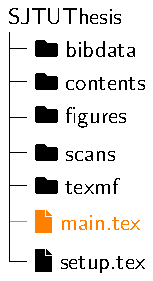
\includegraphics[page=1]{support/figures/thesisdir.pdf}
    \end{column}
    \begin{column}{0.65\textwidth}
      文档类选项是指在载入文档类时的可选选项,多个选项使用逗号隔开,文档类选项会对所有宏包可见。
      \begin{codeblock}[escapechar="]{main.tex}
% !TeX encoding = UTF-8

% 载入 SJTUThesis 模版
"\highlightline"\documentclass[type=master]{sjtuthesis}
% 选项
%   type=[doctor|master|bachelor],
%   zihao=[-4|5],
%   lang=[zh|en],
%   review,
%   [twoside|oneside],
%   math-style=[ISO|TeX],
      \end{codeblock}
    \end{column}
  \end{columns}
\end{frame}

\begin{frame}[fragile]
  \frametitle{文档类选项}
  \begin{columns}
    \begin{column}{0.3\textwidth}
      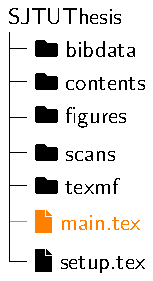
\includegraphics[page=1]{support/figures/thesisdir.pdf}
    \end{column}
    \begin{column}{0.7\textwidth}
      我是学士,写英文论文
      \begin{codeblock}[]{}
|\phantom{}|\documentclass[type=bachelor,lang=en]{sjtuthesis}
      \end{codeblock}
      我是硕士,盲审
      \begin{codeblock}[]{}
|\phantom{}|\documentclass[type=master,review]{sjtuthesis}
      \end{codeblock}
      我是博士,先写着电子版不空页
      \begin{codeblock}[]{}
|\phantom{}|\documentclass[type=doctor,oneside]{sjtuthesis}
      \end{codeblock}
    \end{column}
  \end{columns}
  \note{有 ChatGPT 那味了。}
\end{frame}

\begin{frame}
  \frametitle{文档类选项}
  \begin{columns}
    \begin{column}{0.35\textwidth}
      \includegraphics[page=2,scale=0.9]{support/figures/thesisdir.pdf}
    \end{column}
    \begin{column}{0.65\textwidth}
      \begin{table}
        \caption{文档类选项}
        \footnotesize
        \begin{tabular}{>{\ttfamily}rll}
          \toprule
          选项 & 含义 & 相关 \\
          \midrule
          type= & 指定论文类型 & 第 \ref{covers} 页\\
          \midrule
          cjk-font= & 指定中文字体 & \\
          text-font= & 指定西文字体 & 第 \ref{frame:fonts} 页\\
          math-font= & 指定数学字体 & \\
          math-style= & 指定数学样式 & 第 \ref{frame:math-style} 页\\
          \midrule
          review & 开启盲审模式 & \thesisissue{195} \thesisissue{686} \\
          twoside & 双页模式 & \thesisissue{554} \\
          oneside & 单页模式 & \thesisissue{694} \\
          openright & 章从奇数页开始 & \thesisdiscuss{724} \\
          openany & 章从任意页开始 & \thesisissue{446} \\
          \bottomrule
        \end{tabular}
      \end{table}

      更多文档类选项查阅 \textsc{SJTU\TeX{}} 的开发文档 \link{https://github.com/sjtug/SJTUTeX/releases/download/v1.1.0/sjtuthesis.pdf}。
    \end{column}
  \end{columns}
\end{frame}

\begin{frame}[label={frame:fonts}]
  \frametitle{字体配置}
  \newcommand{\noticemark}{\alert{\normalshape \textopenbullet}}
  \begin{columns}
    \begin{column}{0.35\textwidth}
      \includegraphics[page=3,scale=0.9]{support/figures/thesisdir.pdf}
    \end{column}
    \begin{column}{.65\textwidth}
      相较于 \CTeX{} 使用 \texttt{fontset} 设定中文字体集,
      \SJTUThesis{} 还提供了西文、数学字体集的设定\footnotemark。

      {
        \medskip
        \ttfamily\scriptsize
        \alert{cjk-font=...\hfill 中文字体}
        
        \stamphrule\medskip

        \foreach \sjtufontname/\sjtufontdesc in {adobe/{adobe \faAdobe\noticemark},{fandol}/{fandol \faLinux{} \noticemark},{founder},mac/{mac \faApple{} \noticemark},windows/{windows \faWindows},ubuntu/{ubuntu \noticemark}}{
          \begin{minipage}{2.2cm}
            \centering
            \includefontpreview{support/thesis/cjkfont-\sjtufontname.pdf}\\
            \raisebox{0.8ex}{\sjtufontdesc}
          \end{minipage}
        }

        \bigskip

        \alert{text-font=..., math-font=...\hfill 西文与数学字体}

        \stamphrule\medskip

        \foreach \sjtufontname/\sjtufontdesc in {{cambria}/{cambria \noticemark},{lm},{newcm}/{newcm \noticemark},{newpx},{newtx},{stixtwo}/{stixtwo \noticemark},{times},{xits}/{xits \noticemark}}{
          \begin{minipage}{2cm}
            \centering
            \includefontpreview{support/thesis/latinfont-\sjtufontname.pdf}\\
            \raisebox{0.8ex}{\sjtufontdesc}
          \end{minipage}
        }
      }
    \end{column}
  \end{columns}
  \footnotetext{\noticemark 表示无法使用 pdf\LaTeX{} 编译。}
\end{frame}

\begin{frame}[label={frame:math-style}]
  \frametitle{数学样式}
  \begin{columns}
    \begin{column}{0.35\textwidth}
      \includegraphics[page=2,scale=0.9]{support/figures/thesisdir.pdf}
    \end{column}
    \begin{column}{0.65\textwidth}
      新增数学样式 \texttt{math-style} 文档类选项,现在默认为 \texttt{ISO},
      如果更喜欢原始的 \TeX{} 数学样式,可以切换为 \texttt{TeX}。

      \begin{minipage}[c]{10em}
        \texttt{math-style=ISO}
      \end{minipage}
      \begin{minipage}[c]{5cm}
        \includemathstylepreview{support/thesis/mathstyle-ISO.pdf}
      \end{minipage}
       
      \begin{minipage}[c]{10em}
        \texttt{math-style=TeX}
      \end{minipage}
      \begin{minipage}[c]{5cm}
        \includemathstylepreview{support/thesis/mathstyle-TeX.pdf}
      \end{minipage}

      \begin{block}{}
        请注意在默认情况下(\texttt{math-style=ISO})应当使用 \cmd{increment} 而不是 \cmd{Delta} 表示有限增量。
      \end{block}
    \end{column}
  \end{columns}
\end{frame}

\begin{frame}[fragile]
  \frametitle{基本配置}
  \begin{columns}
    \begin{column}{0.35\textwidth}
      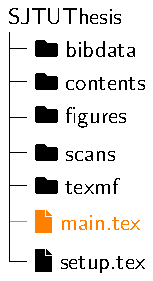
\includegraphics[page=1]{support/figures/thesisdir.pdf}
    \end{column}
    \begin{column}{0.65\textwidth}

      \only<1>{
        在 \texttt{main.tex} 中引入 \texttt{setup.tex} 来导入主要的信息录入与宏包加载配置。
      }

      \only<2>{
        \alert{\textbf{(a,b)}} 其中 \cmd{sjtusetup}(第 \ref{sjtusetup} 页)中的 \opt{info} 将会修改封面的信息设置。
      }

      \begin{codeblock}[firstnumber=12]{main.tex}
|\highlightline<1>|% 论文基本配置,加载宏包等全局配置
|\highlightline<1>|\input{setup}

\begin{document}

%TC:ignore

|\highlightline<2>|% 标题页
|\highlightline<2>|\maketitle
      \end{codeblock}
    \end{column}
  \end{columns}
\end{frame}

\begin{frame}[fragile, label=sjtusetup]
  \frametitle{基本配置}
  \begin{columns}
    \begin{column}{0.35\textwidth}
      \includegraphics[page=4]{support/figures/thesisdir.pdf}
    \end{column}
    \begin{column}{0.65\textwidth}
      \vspace*{-0.2cm}
      \begin{codeblock}[firstnumber=3]{setup.tex}
\sjtusetup{
  info = {
    zh/title  = {|\phantom{}|上海交通大学学位论文 \LaTeX{} 模板示例文档},
    en/title  = {A Sample for \LaTeX-based SJTU Thesis Template},
    zh/author = {|\phantom{}|某\quad{}某},
    en/author = {Mo Mo},
  },
  style = { float-seperator = {--}, },
  name = {
    achv = {|\phantom{}|攻读学位期间完成的论文},
  },
}
      \end{codeblock}
    \end{column}
  \end{columns}
\end{frame}

\begin{frame}[label=setup]
  \frametitle{基本配置}
  \begin{columns}
    \begin{column}{0.35\textwidth}
      \includegraphics[page=4]{support/figures/thesisdir.pdf}
    \end{column}
    \begin{column}{0.65\textwidth}
      \begin{table}
        \centering
        \caption{info 域}
        \footnotesize
        \begin{tabular}{lll} \toprule
          命令作用     & 中文对应选项                      & 英文对应选项                 \\ \midrule
          论文标题     & \texttt{zh/title}                 & \texttt{en/title}            \\
          关键字列表   & \texttt{zh/keywords}              & \texttt{en/keywords*}        \\
          作者姓名     & \texttt{zh/author}                & \texttt{en/author}           \\
          申请学位名称 & \texttt{zh/degree}                & \texttt{en/degree}           \\
          院系名称     & \texttt{zh/department}            & \texttt{en/department}       \\
          专业名称     & \texttt{zh/major}                 & \texttt{en/major}            \\
          导师         & \texttt{zh/supervisor}            & \texttt{en/supervisor}       \\
          副导师       & \texttt{zh/assoc-supervisor}      & \texttt{en/assoc-supervisor} \\
          联培导师     & \texttt{zh/co-supervisor}         & \texttt{en/co-supervisor}    \\
          日期         & \multicolumn{2}{c}{\texttt{date}}                                \\
          学号         & \multicolumn{2}{c}{\texttt{id}}                                  \\ \bottomrule
        \end{tabular}
      \end{table}
    \end{column}
  \end{columns}
  \note{有些选项是 v2 更名或新增的。}
  \note{注意现在使用语言前缀作为键名。}
\end{frame}

\begin{frame}[fragile]
  \frametitle{版权页}
  \begin{columns}
    \begin{column}{0.4\textwidth}
      \includegraphics[page=5]{support/figures/thesisdir.pdf}
    \end{column}
    \begin{column}{0.6\textwidth}
      \alert{\textbf{(c)}} \cmd{copyrightpage} 可以用于插入版权页。
      也可接受一个可选参数,用于直接使用扫描件,此时需要载入 \pkg{pdfpages} 包。\thesisissue{473}

      \begin{codeblock}[firstnumber=22]{main.tex}
% 原创性声明及使用授权书
\copyrightpage
% 插入外置原创性声明及使用授权书
% 导言区添加 \usepackage{pdfpages}
% \copyrightpage[scans/sample-copyright-old.pdf]
      \end{codeblock}
    \end{column}
  \end{columns}
\end{frame}

\begin{frame}[fragile]
  \frametitle{三个部分}
  \framesubtitle{前置部分}
  \begin{columns}
    \begin{column}{0.4\textwidth}
      \includegraphics[page=8]{support/figures/thesisdir.pdf}
    \end{column}
    \begin{column}{0.6\textwidth}
      \alert{\textbf{(d,e,f,g,h)}} 前言从 \cmd{frontmatter} 处开始,页码设置为大写罗马数字,主要包含摘要和目录内容。
      \begin{codeblock}[firstnumber=27]{main.tex}
|\highlightline|% 前置部分
|\highlightline|\frontmatter

% 摘要
\input{contents/abstract}

% 目录
\tableofcontents
% ...
      \end{codeblock}
    \end{column}
  \end{columns}
\end{frame}

\begin{frame}[fragile]
  \frametitle{三个部分}
  \framesubtitle{正文部分}
  \begin{columns}
    \begin{column}{0.4\textwidth}
      \includegraphics[page=9]{support/figures/thesisdir.pdf}
    \end{column}
    \begin{column}{0.6\textwidth}
      \alert{\textbf{(i,j,k)}} 正文从 \cmd{mainmatter} 处开始,页码设置为正常数字,包含正文、参考文献、附录内容。
      \begin{codeblock}[firstnumber=47]{main.tex}
|\highlightline|% 主体部分
|\highlightline|\mainmatter

% 正文内容
\input{contents/intro}
\input{contents/math_and_citations}
\input{contents/floats}
\input{contents/summary}

%TC:ignore

% 参考文献
\printbibliography[heading=bibintoc]

% 附录
\appendix
      \end{codeblock}
    \end{column}
  \end{columns}
\end{frame}

\begin{frame}[fragile]
  \frametitle{三个部分}
  \framesubtitle{结尾部分}
  \begin{columns}
    \begin{column}{0.4\textwidth}
      \includegraphics[page=10]{support/figures/thesisdir.pdf}
    \end{column}
    \begin{column}{0.6\textwidth}
      \alert{\textbf{(k,l,m,n)}} 结尾从 \cmd{backmatter} 处开始,页码设置为正常数字,包含致谢等相关情况。
      \begin{codeblock}[firstnumber=71]{main.tex}
|\highlightline|% 结尾部分
|\highlightline|\backmatter

% 用于盲审的论文需隐去致谢、发表论文、科研成果、简历

% 致谢
\input{contents/acknowledgements}

% 发表论文及科研成果
% 盲审论文中,发表论文及科研成果等仅以第几作者注明即可,不要出现作者或他人姓名
\input{contents/achievements}

%...
      \end{codeblock}
    \end{column}
  \end{columns}
\end{frame}

\begin{frame}
  \frametitle{数学定理环境}
  \begin{columns}
    \begin{column}{0.4\textwidth}
      \includegraphics[page=6]{support/figures/thesisdir.pdf}
    \end{column}
    \begin{column}{0.6\textwidth}
      \SJTUThesis{} 定义了常用的数学环境(需要引入 \pkg{ntheorem} 或者 \pkg{amsthm} 宏包)。

      \begin{table}
        \centering
        \caption{\textsc{SJTUThesis} 定义的数学环境}
        \footnotesize
        \begin{tabular}{>{\ttfamily}rl|>{\ttfamily}rl}
          \toprule
          assumption  & 假设  & lemma       & 引理 \\
          axiom       & 公理  & problem     & 问题 \\
          conjecture  & 猜想  & proof       & 证明 \\
          corollary   & 推论  & proposition & 命题 \\
          definition  & 定义  & remark      & 注   \\
          example     & 例    & solution    & 解   \\
          exercise    & 练习  & theorem     & 定理 \\
          \bottomrule
        \end{tabular}
      \end{table}
    \end{column}
  \end{columns}
\end{frame}

\begin{frame}[fragile]
  \frametitle{参考文献}
  \begin{columns}
    \begin{column}{0.4\textwidth}
      \includegraphics[page=7]{support/figures/thesisdir.pdf}
    \end{column}
    \begin{column}{0.6\textwidth}
      \begin{codeblock}[firstnumber=111,numbersep=2pt]{setup.tex}
% 使用 BibLaTeX 处理参考文献
%   biblatex-gb7714-2015 常用选项
%     gbnamefmt=lowercase     姓名大小写由输入信息确定
%     gbpub=false             禁用出版信息缺失处理
\usepackage[backend=biber,style=gb7714-2015]{biblatex}
% 文献表字体
% \renewcommand{\bibfont}{\zihao{-5}}
% 文献表条目间的间距
\setlength{\bibitemsep}{0pt}
|\highlightline|% 导入参考文献数据库
|\highlightline|\addbibresource{bibdata/thesis.bib}
      \end{codeblock}
    \end{column}
  \end{columns}
\end{frame}

\begin{frame}
  \frametitle{Word}
  \begin{itemize}
    \item[{\faQuestionCircle[regular]}] 跟 Word 的参考实现略有不同 
    \item[{\faCheckCircle[regular]}] 毕设论文的格式只要不违背《上海交通大学关于本科生毕业设计(论文)工作的指导意见》\link{https://github.com/sjtug/SJTUThesis/files/6505296/default.pdf} \thesisissue{621}、《上海交通大学博士、硕士学位论文撰写指南》\link{https://www.gs.sjtu.edu.cn/info/1143/5801.htm} \thesisissue{652} 即可,其他细节上的修改可以先搜索解决方案,再反馈给我们。
    \item[{\faQuestionCircle[regular]}] 我需要转为 Word 文档
    \item[{\faCheckCircle[regular]}] PDF 转为 Word 文档属于逆向工程,暂时不存在完全正确的转换方法 \link{https://www.bilibili.com/video/BV1Vi4y1C71M},从 \LaTeX{} 源代码出发的转换可以使用其他工具实现 \thesisissue{480} \thesisissue{500}。
  \end{itemize}
\end{frame}

\begin{frame}
  \frametitle{还有其他问题?}
  % \begin{columns}
    % \begin{column}{0.73\textwidth}
      \begin{itemize}
        \item[{\faComment*[regular]}] 日常模板或 \LaTeX{} 使用问题可以前往 Discussions \link{https://github.com/sjtug/SJTUThesis/discussions} 提问

        (解决后别忘了 \textcolor{green}{\faCheckCircle{} Mark as answer}
        \item[{\faDotCircle[regular]}] 如果是 \textsc{SJTUThesis} 项目本身的 bug 和 feature request

        可以通过 Issues \link{https://github.com/sjtug/SJTUThesis/issues} 反馈。
        \item[{\faCodeBranch}] 如果你有好点子,可以贡献代码

          向 \textsc{SJTU\TeX{}} \link{https://github.com/sjtug/SJTUTeX} 存储库发 PR,\par
          而后把解包结果同步到 \textsc{SJTUThesis}。
        
        \item[{\faQq}] 也欢迎在 QQ 群(715273806)即时讨论。
        \note{群之前满了,社长给腾讯充了钱,让它可以接着塞人。}
      \end{itemize}
    % \end{column}
    % \begin{column}{0.27\textwidth}
    %   
\includegraphics[height=0.7\textheight]{support/images/qq.jpg}
    % \end{column}
  % \end{columns}
\end{frame}

\end{document}
      \end{codeblock}
    \end{column}
  \end{columns}
  \note<3>{当然,如果需要不换页插入源代码就不用 \cmd{include} 了,
  因为这最主要的好处在于能够在组建大型文档的时候,得到当前页码、编号的进度信息。
  在插入小部件时,还是推荐使用 \cmd{input},这个命令不会额外地产生 \texttt{.aux} 文件,
  对于 I/O 反应慢的(说的就是 \faWindows{})比较友好。}
\end{frame}

\begin{frame}[fragile]
  \frametitle{组织文档}
  \begin{columns}
    \begin{column}{0.4\textwidth}
      \begin{codeblock}[]{learnlatex.tex}
|\highlightline|\chapter{|\phantom{}|学习 \LaTeX{}}
\section{|\phantom{}|概念}
\subsection{\LaTeX{}}
\LaTeX{} 是一个用以排版高质量作品的文档准备系统。
      \end{codeblock}
      子文件中就不需要添加 \env{document} 环境了\footnotemark。
    \end{column}
    \begin{column}{0.6\textwidth}
      \begin{codeblock}[]{主文档 main.tex}
|\highlightline|\documentclass{ctexrep}
\includeonly{learnlatex,sjtuthesis}
\begin{document}
  \tableofcontents
  % !TeX root = ../../latex-talk.tex

\part{学习 \LaTeX{}}
% FIXME: footnote fault numbering
% FIXME: section pop up in navigation in advance

\begin{frame}
  \frametitle{本部分主要参考}
  \begin{bibliolist}{00}
    \onlineitem 陈晟祺~等.
    \newblock 如何使用 \LaTeX\ 排版论文[EB/OL].
    \newblock 2021. \url{https://github.com/tuna/thulib-latex-talk}.

    \onlineitem 曾祥东.
    \newblock 现代 \LaTeX\ 入门讲座[EB/OL].
    \newblock 2022. \url{https://github.com/stone-zeng/latex-talk}.

    \onlineitem \LaTeX\ Project.
    \CTeX\ 开发小组~译.
    \newblock learnlatex.org[EB/OL].
    \newblock 2022. \url{https://github.com/CTeX-org/learnlatex.github.io}.
  
    \onlineitem \textsc{Oetiker T}, \textsc{Partl H}, \textsc{Hyna I}, \textsc{Schlegl E}.
    \CTeX\ 开发小组~译.
    \newblock 一份(不太)简短的 \LaTeXe{} 介绍:或 111 分钟了解 \LaTeXe{}[EB/OL]. \newblock\newblock 2021.
    \url{https://ctan.org/pkg/lshort-zh-cn}.
  \end{bibliolist}

  \note{推荐大家去阅读这些入门材料。}
\end{frame}

\begin{frame}[plain]
  \vfil
  \begin{center}
    \href{https://learnlatex.org}{
      \rmfamily
      Learn\,\lower1ex\hbox{\Huge\LaTeX{}}.org
    }
  \end{center}
  \vfil
  \begin{center}
    \parbox{0.75\linewidth}{
      Learn\LaTeX{}.org 提供了解 \LaTeX{} 的 16 篇简短的教程,并包含了一些可以在线运行的示例,可以通过亲自动手查看实验效果。本部分主要参考由 \CTeX{}-org 提供的中文翻译版本 \link{https://github.com/CTeX-org/learnlatex.github.io/tree/zh-Hans/zh-Hans/}。
    }
  \end{center}
  \vfil
  \note{这一部分主要参考了 Learn\LaTeX{}.org 的系列教程,内容简洁,适合入门,符合
  教育学观念 \link{https://www.tug.org/TUGboat/tb41-2/tb128reviews-learnlatex.pdf},
  并参考由 \CTeX{}-org 提供的中文翻译版本
  \link{https://github.com/CTeX-org/learnlatex.github.io/tree/zh-Hans/zh-Hans/}。
  如果你认为下面一个小时的入门教程没有讲得非常细致的话,
  欢迎直接阅读这个网站的全文。}
\end{frame}

\begin{shadedsection}

\section{是什么}
\begin{frame}
  \frametitle{\TeX{}}
  \begin{columns}[c]
    \begin{column}{0.7\textwidth}
      \begin{center}
        \rmfamily\Huge
        \hologo{La}\highlight[structure!70]{\TeX{}}
      \end{center}
      \begin{center}
        \parbox{0.75\textwidth}{
          \TeX{} 是由斯坦福大学教授高德纳
          (Donald E.~Knuth)于 1977 年开始开发的排版引擎。目前仍在更新,最新版本号为 3.141592653 \link{https://tug.org/TUGboat/tb42-1/tb130knuth-tuneup21.pdf}。
        }
      \end{center}
    \end{column}
    \begin{column}{0.3\textwidth}
      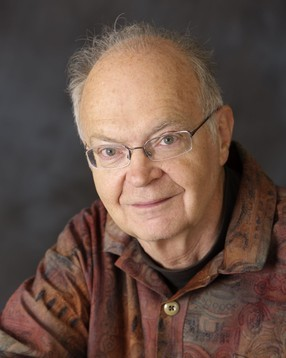
\includegraphics[width=.8\columnwidth]{support/images/Knuth.jpg}
    \end{column}
  \end{columns}
  \note{\emph{这一部分背景介绍大家可以了解一下,暂时跳过。}
  \LaTeX{} 这个词由两个部分组成,\hologo{La} 和 \TeX{}。那我们首先了解一下 \TeX{} 是什么。
  \TeX{} 是由斯坦福大学的教授高德纳于 1977 年开始开发的排版引擎,它已经有三十多年的历史了,
  目前仍在更新,版本号(3.141592653)将会趋近于 $\pi$ 的取值,高德纳最近还在给 \textsl{TUGBoat} 写稿子
  \link{https://tug.org/TUGboat/tb42-1/tb130knuth-tuneup21.pdf},
  关于 \TeX{} 今年又做了哪些改进。}
\end{frame}

\begin{frame}
  \frametitle{\LaTeX{}}
  \begin{columns}[c]
    \begin{column}{0.7\textwidth}
      \begin{center}
        \rmfamily\Huge
        \highlight[structure]{\LaTeX{}}
      \end{center}
      \begin{center}
        \parbox{0.75\textwidth}{
          \LaTeX{} 是最早在 1985 年由现就职于微软的 Leslie Lamport 开发的一种 \TeX{} \textbf{格式}\footnotemark,使用一些列宏和扩展宏包来简化 \TeX{} 的使用。现在由 \LaTeX{} Project 的成员维护。现在广泛使用的版本是 \LaTeXe{},最新的版本为 \LaTeX3(2020 年 10 月后默认内置)。
        }
      \end{center}
    \end{column}
    \begin{column}{0.3\textwidth}
      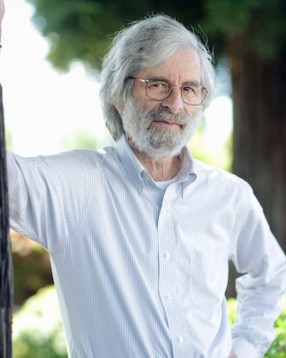
\includegraphics[width=.8\columnwidth]{support/images/Lamport.jpg}
    \end{column}
  \end{columns}
  \footnotetext{\hologo{ConTeXt} 也是一种 \TeX{} 格式 \link{https://www.contextgarden.net/}。}
  \note{\emph{这一部分的背景介绍大家可以了解一下,暂时跳过。}
  \LaTeX{} 是最早由现就职于微软的 Leslie Lamport 开发的一种 \TeX{} 格式(与其对标的是
  \hologo{ConTeXt}\link{https://www.contextgarden.net/}),主要也是为了简化 \TeX{} 的使用。
  现在主要由 \LaTeX{} 开发组维护,现在广泛使用的版本是 \LaTeXe{},最新的版本为 \LaTeX3,
  在 2020 年 10 月后默认内置,所以要尽可能使用较新的发行版,以充分发挥其功能。}
\end{frame}

\begin{frame}
  \frametitle{程序}
  \begin{columns}[c]
    \begin{column}{0.7\textwidth}
      \begin{center}
        \rmfamily\Huge
        \highlight[structure]{\hologo{pdfLaTeX}}
      \end{center}
      \begin{center}
        \parbox{0.7\textwidth}{
          \hologo{pdfLaTeX} 是为了编译一个 \LaTeX{} 文档而运行的程序。实际上底层在运行一个叫 \hologo{pdfTeX} 的引擎,并预装了对应的 \LaTeX{} \textbf{格式}。为了利用临时文件,可能就需要多次运行程序。
        }
      \end{center}
    \end{column}
    \begin{column}{0.3\textwidth}
      \begin{block}{}
        \ttfamily\small
        > \highlight{pdflatex} main.tex\\
        This is pdfTeX, Version 3.141592653-
        2.6-1.40.23 (MiKTeX 21.10)\\
        entering extended mode\\
        \highlight{LaTeX2e} <2021-11-15>\\
        \highlight{L3} programming layer <2021-11-22>
      \end{block}
    \end{column}
  \end{columns}
  \note{\hologo{pdfLaTeX} 是为了编译一个 \LaTeX{} 文档而运行的程序。}
\end{frame}

\begin{frame}
  \frametitle{引擎}
  \begin{columns}[c]
    \begin{column}{0.7\textwidth}
      \begin{center}
        \rmfamily\Huge
        \highlight[structure!70]{pdf}\hologo{La}\highlight[structure!70]{\TeX{}}
      \end{center}
      \begin{center}
        \parbox{0.7\textwidth}{
          pdf\TeX{} 是编译 \TeX{} 文档(以 \texttt{.tex} 结尾)的\textbf{引擎}---可以理解 \TeX{} 指令的\textbf{程序}。
        }
      \end{center}
    \end{column}
    \begin{column}{0.3\textwidth}
      \begin{block}{}
        \ttfamily\small
        > pdflatex main.tex\\
        This is \highlight[structure!70]{pdfTeX}, Version 3.141592653-
        2.6-1.40.23 (MiKTeX 21.10)
        entering extended mode\\
        LaTeX2e <2021-11-15>\\
        L3 programming layer <2021-11-22>
      \end{block}
    \end{column}
  \end{columns}
  \note{实际上底层在运行一个叫 \hologo{pdfTeX} 的引擎,并预装了对应的 \LaTeX{} 格式。}
\end{frame}

\begin{frame}[label={frame:engine}]
  \frametitle{Unicode 引擎}
  \begin{table}
    \caption{主流 \hologo{(La)TeX} 程序
    \footnote{(u)p\TeX{} 是日语最常用的引擎,生成 \texttt{.dvi},支持 Unicode。}\footnote{Ap\TeX{} \link{https://github.com/clerkma/ptex-ng} 具有底层 CJK 支持,内联 Ruby,Color Emoji。}}
    \footnotesize
    \begin{stampbox}
      \begin{tabular}{c>{\raggedright}*{3}{p{3.5cm}}}
        \alert{引擎}     & \hologo{pdfTeX}   & \hologo{XeTeX}   & \hologo{LuaTeX}   \\
        \alert{程序}     & \hologo{pdfLaTeX} & \hologo{XeLaTeX} & \hologo{LuaLaTeX} \\
        \alert{特点}     & 直接生成 PDF,支持 micro-typography  & 支持 Unicode、OpenType 与复杂文字编排 (CTL) & 支持 Unicode,内联 Lua,支持 OpenType \\
      \end{tabular}
    \end{stampbox}
  \end{table}

  \begin{center}
    \parbox{.9\textwidth}{
      \hologo{pdfLaTeX} 不支持 Unicode。为了排版中文,大部分情况下 \faApple{}\,\faLinux{} 应当使用 \hologo{XeLaTeX},而 \hologo{LuaLaTeX} 速度相对较慢。\faWindows{} 可以在一些情况下使用 \hologo{pdfLaTeX}。
    }
  \end{center}
  \note{当然为了排版中文,已经不再推荐使用 \hologo{pdfLaTeX} 了,应该使用 
  \hologo{XeLaTeX} 或者 \hologo{LuaLaTeX},当然后者的速度还是相对较慢,
  它们支持 Unicode 编码,并可以使用 OpenType 字体的全部功能。
  当然 \faWindows{} 平台下在某些追求速度的情况下,
  还是可以试着使用 \hologo{pdfLaTeX} 的。
  
  \hologo{LuaLaTeX} 理想情况下不慢,但是使用一些宏包后会破坏理想状态,
  也会因配置产生不同的结果,不同的操作系统在 I/O 速度上的不同也会导致不同的时间。

  \hologo{pdfLaTeX} 也支持,只不过需要先生成 tfm \TeX{} 字体度量文件,后续使用 \TeX{} 
  自身的配置方法,只能使用 7 比特或 8 比特字体。}
\end{frame}

% \begin{frame}
%   \paragraph{\hologo{pdfLaTeX}} \TeX{} 和 \LaTeX{} 被广泛使用之前,它们只需内置支持欧洲语言即可。在 Unicode 出现之前,\LaTeX{} 提供了许多种\textbf{文件编码}来允许很多语言的文字以原生的方式输入,\hologo{pdfLaTeX} 也只需要使用 8 位文件编码和 8 位字体。
% \end{frame}

\section{跑起来}
\begin{frame}
  \frametitle{发行版}
  \begin{table}
    \caption{\hologo{TeX} 发行版}
    \footnotesize
    \begin{stampbox}
      \begin{tabular}{c>{\raggedright}*{3}{p{3.2cm}}}
        \alert{发行版}     & \hologo{MiKTeX} \link{https://mirrors.sjtug.sjtu.edu.cn/ctan/systems/win32/miktex/setup/windows-x64/}   & \TeX{} Live \link{https://mirrors.sjtug.sjtu.edu.cn/ctan/systems/texlive/Images/}   & Mac\TeX{} \link{https://mirrors.sjtug.sjtu.edu.cn/ctan/systems/mac/mactex/}  \\[2pt]
        \alert{特点}      &  只安装必要文件,依赖用时更新  &  所有平台均可使用,每年发布一次 & Mac 系统专用,对 \TeX{} Live 的进一步打包 \\
        \alert{推荐平台}  & \faWindows  & \faLinux &  \faApple \\
      \end{tabular}
    \end{stampbox}
  \end{table}
  \begin{center}
    \parbox{.9\textwidth}{
      要让 \LaTeX{} 跑起来,核心就是要有一套 \TeX{} 发行版,来获取让 \LaTeX{} 工作所需的一组程序和文件。参考《一份简短的关于 \LaTeX{} 安装的介绍》\link{https://mirrors.sjtug.sjtu.edu.cn/ctan/info/install-latex-guide-zh-cn/install-latex-guide-zh-cn.pdf} 安装想使用的发行版。推荐使用发行版的最新版本\footnote{老版本 Linux 系统的包管理器自带 \TeX{} Live 发行版可能不是最新的 \link{https://repology.org/project/texlive/versions},尽量使用镜像安装,并手动将相关环境变量添加到路径 \link{https://www.tug.org/texlive/doc/texlive-zh-cn/texlive-zh-cn.pdf}。},并使用国内镜像。
    }
  \end{center}
  \note{要让 \LaTeX{} 跑起来,核心就是要有一套 \TeX{} 发行版,来获取让 
  \LaTeX{} 工作所需的一组程序和文件。参考《一份简短的关于 \LaTeX{} 安装的介绍》
  安装想使用的发行版,里面介绍了 \faWindows{}, \faApple{}, \faLinux{}, WSL 等系统上
  \TeX{} Live 的安装,非常全面,一步一步做就可以成功安装。目前最新的 \TeX{} Live 版本为
  2022,\SJTUThesis{} 用户不应当安装 \TeX{} Live 2020 以下的版本(后面会讲)。
  
  事实上,我认为这几个发行版各有操作系统偏好,虽然前两者是跨平台的。

  \hologo{MiKTeX} 对 Windows 用户较为友好,安装简单,占用空间不大,安装时间短,
  而且有完整的安装与卸载程序。可以给大家看一下 \hologo{MiKTeX} Console 的情况。

  \TeX{} Live 更符合 Linux 的更新传统。老版本 Linux 系统的包管理器自带 \TeX{} Live
  发行版可能不是最新的(到时间也会锁定依赖库的版本),尽量使用镜像安装(当然也推荐使用最新的
  Linux 发行版,这样它的版本也就一直是最新的),并手动将相关环境变量添加到路径。

  Mac\TeX{} 发行版有 pkg 安装包封装,并且附带了 \TeX{}Shop 基本编辑软件,更加适合 Mac OS。
  我用下来的话,感觉除了 \TeX{} Live Utility 外都有点过时了。}
\end{frame}

\begin{frame}[plain]
  \hbox to \textwidth{
    \hfil
    \vbox to 3cm{
      \hbox{
        \resizebox{3cm}{!}{
\includegraphics{support/examples/pics/sjtug}}
      }
    }
    \hfil
    \vbox to 3cm{
      \vfill
      \hbox{\Large\bfseries\color{structure} 稳定、快速、现代的镜像服务。}
      \vskip2pt
      \hbox{托管于华东教育网骨干节点上海交通大学。}
      \vfill
    }
    \hskip20pt
    \hfil
  }

  \begin{center}
    \parbox{0.8\textwidth}{
      推荐使用 SJTUG 软件镜像服务 \link{https://mirror.sjtu.edu.cn/},离得近,下得快。
      
      \begin{description}
        \footnotesize
        \item[\TeX{} Live]  {\ttfamily tlmgr option repository https://mirrors.sjtug.sjtu.edu.cn/CTAN/systems/texlive/tlnet}
        \item[\hologo{MiKTeX}] 在 \hologo{MiKTeX} Console 中设置镜像源为 \url{https://mirrors.sjtug.sjtu.edu.cn}
        \item[\faTelegram] 可以在 SJTUG 镜像站通知频道 \link{https://t.me/sjtug_mirrors_news} 获得更多信息,加入关联群组参与讨论。
      \end{description}
    }
  \end{center}
  \note{说到镜像,像后两者的安装包都很大(4GB 左右),由于一些原因,不采用镜像的话不知道要下到什么时候,对下载速度的要求高;
  而 \hologo{MiKTeX} 需要随时更新,宏包大小颗粒度大,对延迟的要求高。
  那么采用 SJTUG 镜像源将同时解决这两个问题,位于图信大楼的机房,凭借校内的高速网络,稳定快速下载,
  现在由 LightQuantum 维护的镜像站欢迎大家的使用,主页上还有更多的其他镜像可供使用,加入 Telegram 群组参与讨论。}
\end{frame}

\begin{frame}
  \frametitle{编辑器}
  \begin{table}
    \caption{开源编辑器推荐}
    \footnotesize
    \begin{stampbox}
      \begin{tabular}{c>{\raggedright}*{3}{p{3.5cm}}}
        \alert{编辑器}     & \begin{tabular}{c}Visual Studio Code \link{https://code.visualstudio.com}\\ \LaTeX{} Workshop\end{tabular}  & \TeX{}studio \link{https://texstudio.org} & \TeX{}works \\[5pt]
        \alert{特点}      &  搭配 VS Code 使用非常方便,易扩展  & 可以使用大量的菜单选项输入代码块,用户友好 & 只提供基础的高亮与运行方法,发行版自带\footnote{Mac\TeX{} 打包的是 \TeX{}Shop 编辑器。} \\
      \end{tabular}
    \end{stampbox}
  \end{table}
  \begin{center}
    \parbox{.9\textwidth}{
      使用专为 \LaTeX{} 设计的编辑器将带来更多便利,因为它们往往会提供一键编译、内置 PDF 阅读器以及语法高亮等功能。几乎所有现代的 \LaTeX{} 编辑器都提供 Sync\TeX{} 这一强大的功能,以在 PDF 和代码间对应跳转。
    }
  \end{center}
  \note{编辑器的种类很多,我无法一一列举,但是对编写 \TeX{} 常用的开源编辑器我推荐这三个。
  其中 \TeX{}studio 的安装包可能下得有点慢。这里我对这些编辑器都演示一下,初学者我更推荐使用
  \TeX{} studio 编辑器,如果平时就码很多代码的话,我更推荐使用 VS Code 加插件这种方式。
  
  使用专为 \LaTeX{} 设计的编辑器将带来更多便利,因为它们往往会提供一键编译、内置 PDF 阅读器
  以及语法高亮等功能。几乎所有现代的 \LaTeX{} 编辑器都提供 Sync\TeX{} 这一强大的功能
  (VS Code 的方法是 Ctrl + 某处,Overleaf 的方法是直接双击),以在 PDF 和代码间对应跳转。
  当然如果你不喜欢使用这种 GUI 编辑器,\TeX{} 文档本身就是纯文本,对 Vim, Emacs 等终端用户
  也很友好。}
\end{frame}

\begin{frame}
  \frametitle{在线平台}
  \begin{table}
    \caption{在线协作平台推荐}
    \footnotesize
    \begin{stampbox}
      \begin{tabular}{c>{\raggedright}*{2}{p{4cm}}}
        \alert{在线平台}     & Overleaf \link{https://www.overleaf.com/}  & 交大 \LaTeX{} 助手 \link{https://latex.sjtu.edu.cn/} \\[2pt]
        \alert{特点}      & 最流行的在线平台,提供大量的模板,但国内访问慢 & 校内平台,隐私保护有保障,共享项目限制少 \\
      \end{tabular}
    \end{stampbox}
  \end{table}
  \begin{center}
    \parbox{.9\textwidth}{
      在线平台允许你直接在网页中编辑文档,无需本地安装即可在后台运行 \LaTeX{},并显示生成的 PDF。可以参照 Overleaf 官方文档学习如何使用在线平台 \link{https://www.overleaf.com/learn}。
    }
  \end{center}
  \note{当然使用在线平台省去了安装发行版的麻烦,这里列出两种在线写作平台。

  如果有数据合规需求的话,可以考虑使用由网络信息中心维护的交大 \LaTeX{} 助手,最近更新了 \TeX{} Live 2022,还是很不错的。

  当然国内还有 \TeX{} Page \link{https://www.texpage.com/},Slagger \link{https://www.slager.cn/} 等。
  一般来讲,这种平台使用的都是 Linux 操作系统,所以在排版中文的时候考虑将编译引擎更改为 \hologo{XeLaTeX},
  学习如何使用在线平台参见 Overleaf 的官方文档 \link{https://www.overleaf.com/learn}。}
\end{frame}

\section{基本结构}
\begin{frame}[fragile]%
  \frametitle{文档部件}
  \begin{columns}[c]
    \begin{column}{0.4\textwidth}
      \only<1>{
        \cmd{documentclass} 命令加载了\textbf{文档类}。\cls{article} 是由 \LaTeX{} 提供的用于排版短文档的基本文档类。
        \begin{description}
          \footnotesize
          \item[\cls{article}] 不包含章的短文档
          \item[\cls{report}] 含有章的单面印刷文档
          \item[\cls{book}] 含有章的双面印刷文档
          \item[\cls{beamer}] 幻灯片
        \end{description}
      }

      \only<2>{
        \env{document} 环境用于指示文档主体的范围。\LaTeX{} 还有其他的使用 \cmd{begin} 和 \cmd{end} 的搭配,我们称这些为\textbf{环境}。它们将用来设定局部格式命令\footnotemark。
      }

      \only<3>{
        \includepdflarge{support/examples/enminimal.pdf}
      }
    \end{column}
    \begin{column}{0.6\textwidth}
      \begin{codeblock}[]{排版英文最简示例}
|\highlightline<1>|\documentclass{article}
|\highlightline<2>|\begin{document}
|\highlightline<3>|  Together for a Shared Future
|\highlightline<2>|\end{document}
      \end{codeblock}
    \end{column}
  \end{columns}

  \only<2>{\footnotetext{环境实际上是一个组,只不过通过语义化的形式预装了对应的格式命令。普通的组可以直接使用一对大括号之间的内容 \{$\cdots$\} 表示。}}
\end{frame}

\section{扩展}
\begin{frame}[fragile]%
  \frametitle{中文排版}
  \begin{columns}[c]
    \begin{column}{0.4\textwidth}

      \only<1>{
        \cmd{usepackage} 用于使用宏包以向 \LaTeX{} 添加或修改功能,需要在\textbf{导言区}调用。
        这里使用 \pkg{ctex} 宏集以获得中文支持。其调用底层因不同的引擎而不同。
        \begin{center}
          \footnotesize
          \begin{tabular}{c*{3}{c}}
            \alert{引擎}     & \hologo{pdfTeX}   & \hologo{XeTeX}   & \hologo{LuaTeX}   \\
            \alert{程序}     & \hologo{pdfLaTeX} & \hologo{XeLaTeX} & \hologo{LuaLaTeX} \\
            \alert{宏包}     & CJK\footnotemark & xeCJK & luatexja \\
            \alert{封装}     & \multicolumn{3}{c}{ctex} \\
          \end{tabular}
        \end{center}
        \vspace{-1cm}
      }

      \only<2>{
        \CTeX{} 建议对于之前提到的常规文档类,最佳实践是使用该宏集提供的四种中文文档类,以对特定类型提供额外的中文排版适配。
        \begin{center}
          \footnotesize
          \begin{tabular}{cc}
            \cls{ctexart} & \cls{ctexrep} \\
            \cls{ctexbook} & \cls{ctexbeamer} \\
          \end{tabular}
        \end{center}
      }

      \only<3>{
        \includepdflarge{support/examples/cnminimal.pdf}
      }

      \only<4>{
        大部分情况下,你都不应当在 \LaTeX{} 中强制断行:你几乎只是想另起一段,或者是想在段落之间添加空行(使用 \pkg{parskip} 宏包就可实现)。
        只有\alert{很少的}情况下你需要使用 \textbackslash{}\textbackslash{} 来另起一行而不另起一段(强制断行仍在同一段)。
      }
    \end{column}
    \begin{column}{0.6\textwidth}
      \begin{codeblock}[]{排版中文\only<2->{最佳实践}}
|\highlightline<2>|\documentclass{|\only<1>{article}\only<2->{ctexart}|}
|\only<1>{\highlightline\textbackslash{}usepackage\{ctex\}\hfill\color{structure}\% 导言区}|
\begin{document}
|\highlightline<3>|    一起向未来
|\highlightline<4>|
  Together for a Shared Future
\end{document}
      \end{codeblock}
    \end{column}
  \end{columns}
  \only<1>{\footnotetext{ctex 在 \faApple\,\faLinux{} 上已经不可以使用 \hologo{pdfLaTeX} 编译,以及在 \faWindows{} 上使用该引擎也会变更自动间距调整等功能的默认行为。}}
\end{frame}

\section{设定格式}
\begin{frame}[fragile]%
  \frametitle{字体样式}
  \begin{columns}
    \begin{column}{0.4\textwidth}
      \only<1>{
        \includepdflarge{support/examples/fontstyle.pdf}
      }

      \only<2>{
        可以使用显式样式设定命令对小段做加粗、斜体、等宽等等的处理。
        \begin{center}
          \footnotesize
          \begin{tabular}{rl}
            \cmd{textrm} & \textrm{衬线} \\
            \cmd{textbf} & \textbf{加粗} \\
            \cmd{textit} & \kaishu 斜体 \\
            \cmd{texttt} & \texttt{等宽} \\
            \cmd{textsf} & \textsf{无衬线} \\
            \cmd{textsc} & \textsc{Small Caps} \\
            \cmd{textsl} & \textsl{Slanted} \\
          \end{tabular}
        \end{center}
      }

      \only<3>{
        与 Word 不同的是,\LaTeX{} 一般情况下并不需要使用上面的显式命令,而是采用逻辑标记的方法,
        比如 \cmd{emph} 可以强调文字,以及下面将要提到的目次命令(第 \ref{sectioning} 页)。
        这样可以统一管理格式。
      }
    \end{column}
    \begin{column}{0.6\textwidth}
      \begin{codeblock}[]{样式}
\documentclass{ctexart}
\begin{document}
|\highlightline<2>|  \textbf{|\phantom{}|一起向未来}

|\highlightline<3>|  \emph{Together for a Shared Future}
\end{document}
      \end{codeblock}
    \end{column}
  \end{columns}
\end{frame}

\begin{frame}[fragile]%
  \frametitle{\only<1-2>{字体大小}\only<3>{字体样式}}
  \begin{columns}
    \begin{column}{0.4\textwidth}
      \only<1>{
        \includepdflarge{support/examples/fontsize.pdf}
      }

      \only<2>{
        同样地,你也可以显式地设定字体大小,但是这种命令会更改行文设置,所以需要使用一个组来限定作用范围\footnotemark。
        \begin{center}
          \footnotesize
          \begin{tabular}{rl}
            \cmd{tiny} & \tiny 极小 \\
            \cmd{scriptsize} & \scriptsize 角标大小  \\
            \cmd{footnotesize} & \footnotesize 脚注大小 \\
            \cmd{small} & \small 小 \\
            \cmd{normalsize} & \normalsize 正常大小 \\
            \cmd{large} & \large 大 \\
            \cmd{huge} & \Huge 巨大 \\
          \end{tabular}
        \end{center}
      }

      \only<3>{
        也可以使用字体样式对应的更改字体设置的命令,这对于大段文段的设置而言也是很方便的。
        \begin{center}
          \footnotesize
          \begin{tabular}{ll}
            \cmd{textrm} & \cmd{rmfamily}\\
            \cmd{texttt} & \cmd{ttfamily}\\
            \cmd{textsf} & \cmd{sffamily}\\
            \cmd{textbf} & \cmd{bfseries}\\
            \cmd{textit} & \cmd{itshape}\\
            \cmd{textsc} & \cmd{scshape}\\
            \cmd{textsl} & \cmd{slshape}\\
          \end{tabular}
        \end{center}
      }
    \end{column}
    \begin{column}{0.6\textwidth}
      \begin{codeblock}[]{大小}
\documentclass{ctexart}
\begin{document}
|\highlightline<2>|  {\bfseries\Large 一起向未来\par}
|\highlightline<3>|  {\itshape Together for a Shared Future}
\end{document}
      \end{codeblock}
    \end{column}
  \end{columns}

  \only<2>{\footnotetext{注意最后显式地使用 \cmd{par} 在改回大小前结束该段,否则会导致下一行的行间距异常!}}
\end{frame}

\section{逻辑结构}
\begin{frame}[fragile]
  \frametitle{列表}
  \begin{columns}
    \begin{column}{0.35\textwidth}
      \begin{codeblock}[]{无序列表}
\documentclass{ctexart}
\begin{document}
|\highlightline|  \begin{itemize}
    \item 第一项
    \item 第二项
    \item 第三项
|\highlightline|  \end{itemize}
\end{document}
      \end{codeblock}
    \end{column}
    \begin{column}{0.35\textwidth}
      \begin{codeblock}[]{有序列表}
\documentclass{ctexart}
\begin{document}
|\highlightline|  \begin{enumerate}
    \item 第一项
    \item 第二项
    \item 第三项
|\highlightline|  \end{enumerate}
\end{document}
      \end{codeblock}
    \end{column}
    \begin{column}{0.35\textwidth}
      \begin{codeblock}[]{描述列表}
\documentclass{ctexart}
\begin{document}
|\highlightline|  \begin{description}
    \item[|\phantom{}|第一] 文本
    \item[|\phantom{}|第二] 文本
    \item[|\phantom{}|第三] 文本  
|\highlightline|  \end{description}
\end{document}
      \end{codeblock}
    \end{column}
  \end{columns}
  \note{接下来我们概览一下三种列表:无序列表、有序列表、描述列表。这些列表可以相互嵌套,但最多嵌套四层。}
\end{frame}

%更深的列表技巧,定理环境等

\begin{frame}
  \frametitle{列表}
  \begin{columns}
    \begin{column}{0.35\textwidth}
      \includepdflarge{support/examples/unordered.pdf}
    \end{column}
    \begin{column}{0.35\textwidth}
      \includepdflarge{support/examples/ordered.pdf}
    \end{column}
    \begin{column}{0.35\textwidth}
      \includepdflarge{support/examples/description.pdf}
    \end{column}
  \end{columns}
\end{frame}

\begin{frame}[fragile,label=sectioning]%
  \frametitle{目次结构}
  \begin{columns}
    \begin{column}{0.4\textwidth}
      \LaTeX{} 可以使用目次命令将文档划分层级\footnotemark,并自动设定对应字体样式和大小。
      \begin{center}
        \footnotesize
        \begin{tabular}{rll}
          命令 & 含义 & 层次 \\
          \cmd{chapter} & 章\footnotemark & \sout{0} \\
          \cmd{section} & 节 & 1 \\
          \cmd{subsection} & 小节 & 2 \\
          \cmd{subsubsection} & 小小节 & 3 \\
        \end{tabular}
      \end{center}
    \end{column}
    \begin{column}{0.6\textwidth}
      \begin{codeblock}[]{目次}
\documentclass{ctexart}
\begin{document}
|\highlightline|  \section{|\phantom{}|概念}
|\highlightline|  \subsection{\LaTeX{}}
  \LaTeX{} 是一个用以排版高质量作品的文档准备系统。
\end{document}
      \end{codeblock}
    \end{column}
  \end{columns}
  \footnotetext{章这一级只在 \cls{report} 和 \cls{book} 文档类(包括对应的中文文档类)有定义。还有不常用的 \cmd{part} (0@\cls{article}/-1@\cls{report}\&\cls{book}\&\cls{beamer}) 以及更低层次的 \cmd{paragraph} (4) 与 \cmd{subparagraph} (5)。 }
  \note{而知道层次,对我们下面生成目录有帮助。}
\end{frame}

\begin{frame}[fragile]%
  \frametitle{组织文档}
  \begin{columns}
    \begin{column}{0.4\textwidth}

      \only<1>{
        \cmd{tableofcontents} 用来生成对于目次命令的目录。如果你想设定显示到哪个层级,在这个命令前使用 \cmd{setcounter\{tocdepth\}\{层次\}}

        如果你想在目录中使用更短的标题:

            \cmd{section[短标题]\{长标题\}}

        如果你想让本目次的标题不显示在目录中:

            \cmd{section*\{目录没这个标题\}}
      }

      \only<2>{
        对于大型文档而言,使用多个文件管理源文件通常是更方便的。而 \cmd{include} 和 \cmd{input} 都以相对路径的方式插入其他 \TeX{} 文档。
        区别在于,\cmd{include} 命令会从新页开始并做一些内部调整,这基本上只对 \pkg{chapter} 这一级有用。而 \cmd{input} 会原样插入源代码。
      }

      \only<3>{
        但是 \cmd{include} 插入的文档可以使用 \cmd{includeonly} 管理当前要排印哪一部分的内容,利用所有章节辅助文件的同时,减少编译时间并专注于该部分的内容。
      }
    \end{column}
    \begin{column}{0.6\textwidth}
      \begin{codeblock}[]{主文档}
\documentclass{ctexrep}
|\highlightline<3>|\includeonly{learnlatex,sjtuthesis}
\begin{document}
|\highlightline<1>|  \tableofcontents
|\only<2-3>{\highlightline}|  \include{learnlatex}
|\highlightline<3>|  \include{sjtuthesis}
\end{document}
      \end{codeblock}
    \end{column}
  \end{columns}
  \note<3>{当然,如果需要不换页插入源代码就不用 \cmd{include} 了,
  因为这最主要的好处在于能够在组建大型文档的时候,得到当前页码、编号的进度信息。
  在插入小部件时,还是推荐使用 \cmd{input},这个命令不会额外地产生 \texttt{.aux} 文件,
  对于 I/O 反应慢的(说的就是 \faWindows{})比较友好。}
\end{frame}

\begin{frame}[fragile]
  \frametitle{组织文档}
  \begin{columns}
    \begin{column}{0.4\textwidth}
      \begin{codeblock}[]{learnlatex.tex}
|\highlightline|\chapter{|\phantom{}|学习 \LaTeX{}}
\section{|\phantom{}|概念}
\subsection{\LaTeX{}}
\LaTeX{} 是一个用以排版高质量作品的文档准备系统。
      \end{codeblock}
      子文件中就不需要添加 \env{document} 环境了\footnotemark。
    \end{column}
    \begin{column}{0.6\textwidth}
      \begin{codeblock}[]{主文档 main.tex}
|\highlightline|\documentclass{ctexrep}
\includeonly{learnlatex,sjtuthesis}
\begin{document}
  \tableofcontents
  \include{learnlatex}
  \include{sjtuthesis}
\end{document}
      \end{codeblock}
    \end{column}
  \end{columns}
  \footnotetext{如果想强制指定子文档的主文档,可以在文件第一行输入魔术命令:\texttt{\% !TeX root = main.tex}}
\end{frame}

\section{图}
\begin{frame}[fragile]%
  \frametitle{\temporal<5>{插图}{浮动体}{插图}}
  \begin{columns}
    \begin{column}{0.6\textwidth}
      \begin{codeblock}[]{插入单图\only<4->{最佳实践}}
\documentclass{ctexart}
|\highlightline<2>|\usepackage{graphicx}
|\highlightline<2>|\graphicspath{{figs/}{pics/}}
\begin{document}
|\highlightline<5>|\begin{figure}[ht]
|\highlightline<6>|  \centering
|\highlightline<3>|  
\includegraphics[width=|\only<1-3>{4cm}\only<4->{0.4\textbackslash{}textwidth}|]{sjtug}
|\highlightline<7>|  \caption{SJTUG 徽标}\label{fig:sjtug}
|\highlightline<5>|\end{figure}
\end{document}
      \end{codeblock}
    \end{column}
    \begin{column}{0.4\textwidth}
      \only<1>{
        \includepdflarge{support/examples/insertimage.pdf}
      }

      \only<2>{
        为了插入外部图片,需要使用 \pkg{graphicx} 宏包。之后在文档主体便可以使用 \cmd{includegraphics} 插入图片。导言区也可以加入 \cmd{graphicspath} 指定图片文件夹\footnotemark。
      }

      \only<3>{
        \cmd{includegraphics} 命令便以相对路径的方式插入图片,如果无同名图片,那么后缀名可以省略。可以使用可选参数指定插入的图片尺寸,最佳实践是使用 \cmd{textwidth} 或 \cmd{linewidth} 的相对值指定尺寸大小,以在未来可能的布局更改中保留一定的灵活性。
        \note{比如我未来想变更为幻灯片的时候。}
      }

      \only<4>{
        也可以通过键值对的方法设置图片的其他属性。
        \note{事实上,\LaTeX{} 很多命令都是使用方括号添加可选参数的。}
        \begin{center}
          \footnotesize
          \begin{tabular}{rl}
            \opt{width} & 宽度 \\
            \opt{height} & 高度 \\
            \opt{scale} & 缩放 \\
            \opt{angle} & 角度 \\
          \end{tabular}
        \end{center}
      }

      \only<5>{
        \env{figure} 为一个浮动体环境(\env{table} 也是),可以将其移动到其他位置上以减少行文中的空白。可以添加可选参数以指定如何放置浮动体,最多可以使用四种位置描述符:
        \begin{center}
          \footnotesize
          \begin{tabular}{cll}
            \opt{h} & Here & 尽可能在这里 \\
            \opt{t} & Top & 页面顶部 \\
            \opt{b} & Bottom & 页面底部 \\
            \opt{p} & Page & 浮动体专页 \\
          \end{tabular}
        \end{center}
        还可以只使用 \pkg{float} 宏包提供的 \opt{H} 描述符以强制置于此处。
      }

      \only<6>{
        采用 \cmd{centering} 命令而不是 \env{center} 环境来水平居中图片。这将避免多余的纵向间距。
      }

      \only<7>{
        使用 \cmd{caption} 命令输入题注,如果这个命令写在插入图片前面,题注将会在上方(中文中一般对 \env{table} 环境这么做)。后面将会看到如何对留有标记(\cmd{label})的图片进行引用。
      }
    \end{column}
  \end{columns}
  \only<2>{\footnotetext{其命令参数每个为一个以 \texttt{/} 结尾的文件夹,每个文件夹需要使用大括号包裹起来。}}
\end{frame}

\begin{frame}[fragile]
  \begin{columns}
    \begin{column}{0.6\textwidth}
      \begin{codeblock}[]{插入双图}
\documentclass{ctexart}
\usepackage{graphicx}
\graphicspath{{figs/}{pics/}}
\begin{document}
  \begin{figure}[ht]
|\highlightline<1>|    \begin{minipage}{0.48\textwidth}
      \centering
      
\includegraphics[height=2cm]{sjtug}
|\highlightline<2>|      \caption{SJTUG 徽标}\label{fig:sjtug}
|\highlightline<1>|    \end{minipage}\hfill
|\highlightline<1>|    \begin{minipage}{0.48\textwidth}
      \centering
      
\includegraphics[height=2cm]{sjtugt}
|\highlightline<2>|      \caption{SJTUG|\phantom{}|文字}\label{fig:sjtugt}
|\highlightline<1>|    \end{minipage}
  \end{figure}
\end{document}
      \end{codeblock}
    \end{column}
    \begin{column}{0.4\textwidth}

      \only<1>{
        在 \env{figure} 环境里使用 \env{minipage} 小页制作列盒子,以并排两图并分别编号,需要设定强制参数以指定列宽。两个小页之间添加 \cmd{hfill} 使两个小页两端对齐。
      }

      \only<2>{
        在每个小页内部分别使用 \cmd{caption} 添加标签。
      }

      \only<3>{
        \includepdflarge{support/examples/doubleimages.pdf}
      }
    \end{column}
  \end{columns}
\end{frame}

\begin{frame}[fragile]%
  \begin{columns}
    \begin{column}{0.6\textwidth}
      \begin{codeblock}[]{}
\documentclass{ctexart}
\usepackage{graphicx}
|\highlightline|\usepackage{subcaption}
\graphicspath{{figs/}{pics/}}
\begin{document}
  \begin{figure}[ht]
|\highlightline|    \begin{subfigure}{0.48\textwidth}
      \centering
      
\includegraphics[height=2cm]{sjtug}
      \caption{|\phantom{}|徽标}
|\highlightline|    \end{subfigure}\hfill
|\highlightline|    \begin{subfigure}{0.48\textwidth}
      \centering
      
\includegraphics[height=2cm]{sjtugt}
      \caption{|\phantom{}|文字}
|\highlightline|    \end{subfigure}
    \caption{SJTUG}\label{fig:sjtug}
  \end{figure}
\end{document}
      \end{codeblock}
    \end{column}
    \begin{column}{0.4\textwidth}
      \includepdflarge{support/examples/subfigures.pdf}\vspace{15pt}
      \pkg{subcaption} 宏包提供了 \env{subfigure} 环境(以及 \env{subtable}),可以用于以子图的形式插入,编号会增加一级。也可以为子图添加子级引用编号。
    \end{column}
  \end{columns}
\end{frame}

\section{表}
\begin{frame}[fragile]
  \frametitle{简单表格}
  \begin{columns}
    \begin{column}{0.6\textwidth}
      \begin{codeblock}[]{}
\documentclass{ctexart}
|\only<1-2>{\highlightline}|\usepackage{|\temporal<1>{array}{\highlight{array}}{array},\temporal<2>{booktabs}{\highlight{booktabs}}{booktabs}|}
\begin{document}
\begin{table}[ht]
  \centering
  \caption{|\phantom{}|北京冬奥会吉祥物}
|\highlightline<1>|  \begin{tabular}{lp{3cm}}
|\highlightline<2>|    \toprule
|\highlightline<3>|吉祥物 & 描述                          \\
|\highlightline<2>|    \midrule
|\highlightline<3>|冰墩墩 & 2022 年北京冬季奥运会吉祥物  \\
|\highlightline<3>|雪容融 & 2022 年北京冬季残奥会吉祥物  \\
|\highlightline<2>|    \bottomrule
|\highlightline<1>|  \end{tabular}
\end{table}
\end{document}
      \end{codeblock}
    \end{column}
    \begin{column}{0.4\textwidth}
      
      \only<1>{
        使用 \env{tabular} 环境绘制表格。需要添加参数(称为\textbf{表格导言})以确定每一列的对齐方式。引入 \pkg{array} 宏包来使用更多的\textbf{引导符}。
        \begin{center}
          \footnotesize
          \begin{tabular}{>{\ttfamily}ll}
            \alert{l} & 向左对齐 \\
            \alert{c} & 居中对齐 \\
            \alert{r} & 向右对齐 \\
            \alert{p\{3cm\}} & 固定列宽,两端对齐 \\
            \alert{m\{3cm\}} & \texttt{p} + 垂直居中对齐 \\
            \alert{>\{\textbackslash{}bfseries\}} & 后一列单元格前加命令 \\
            \alert{*\{3\}\{l\}} & 三个左对齐列 \\
          \end{tabular}
        \end{center}
      }

      \only<2>{
        \pkg{booktabs} 宏包提供了标准三线表格所需要的行分割线:\cmd{toprule},\cmd{midrule},\cmd{bottomrule}。也可以使用 \cmd{cmidrule\{1-2\}} 来部分地绘制行分割线。一般不推荐在专业表格中使用纵向分割线。
      }

      \only<3>{
        每行内容使用 \textbackslash\textbackslash{} 分隔开,每行中的单元格使用 \& 分隔开。
      }

      \only<4>{
        \includepdflarge{support/examples/table.pdf}
      }
    \end{column}
  \end{columns}
\end{frame}

\begin{frame}[fragile]%
  \begin{columns}
    \begin{column}{0.6\textwidth}
      \begin{codeblock}[]{表头居中}
\documentclass{ctexart}
\usepackage{array,booktabs}
\begin{document}
\begin{table}[ht]
  \centering
  \caption{|\phantom{}|北京冬奥会吉祥物}
  \begin{tabular}{lp{3cm}}
    \toprule
|\highlightline|\multicolumn{1}{c}{|\phantom{}|吉祥物} &
|\highlightline|\multicolumn{1}{c}{|\phantom{}|描述} \\
    \midrule
|\phantom{}|冰墩墩 & 2022 年北京冬季奥运会吉祥物  \\
|\phantom{}|雪容融 & 2022 年北京冬季残奥会吉祥物  \\
    \bottomrule
  \end{tabular}
\end{table}
\end{document}
      \end{codeblock}
    \end{column}
    \begin{column}{0.4\textwidth}
      \cmd{multicolumn} 命令不仅可以用于合并同行的单元格,还可以用于临时地屏蔽表格导言对该列的对齐方式定义。这里用于居中表头。
      \begin{center}
        \parbox{0.85\linewidth}{
          \cmd{multicolumn\{格数\}\{对齐方式\}\{内容\}}
        }
      \end{center}
      跨页表格考虑使用 \pkg{longtable} 宏包。带标注的表格可以考虑使用 \pkg{threeparttable} 宏包。考虑使用在线工具生成表格代码 \link{https://www.tablesgenerator.com/latex_tables}。
      \note{复杂的使用方法在 \SJTUThesis{} 示例文档中都有提及。}
    \end{column}
  \end{columns}
\end{frame}

\section{数学公式}
\begin{frame}
  \frametitle{数学模式}
  \begin{alertblock}{}
  输入数学公式是 \LaTeX{} 的绝对强项,很多常见的公式服务依赖于一些轻量级渲染引擎比如 MathJax, K\kern-.3ex\raise.4ex\hbox{\footnotesize A}\kern-.3ex\TeX{}。但是它们实际上使用的是 \LaTeX{} 语法变种,也就是说并没有使用 \LaTeX{} 后端。所以不要期望有完全一致的输出。
  \end{alertblock}
  
  为了更好的获得数学公式输入支持,请使用 \hologo{AmS}math 宏包。数学模式分为两种:
  \begin{description}
    \item[行内模式] 一般通过一对美元符号(\$$\cdots$\$)标记,可以使用编辑器内建的符号表输入数学符号,也可以使用在线工具手写识别 \link{https://detexify.kirelabs.org/classify.html}。
    \item[行间模式] 一般通过 \env{equation} 环境\footnote{这是有编号环境,其加星号的变种 \env{equation*} 用于生成无编号环境。}输入。如果需要使用多行公式,请使用 \env{align} 环境,并按照类似表格输入的方式,使用 \& 对齐符号,\textbackslash\textbackslash{} 换行。如果不想手动居中,可以考虑多行自动居中的 \env{gather} 和单个大型公式首尾两端对齐 \env{multline}。
  \end{description}
  \note{关于表格和数学公式,如果不太熟悉如何输入,或者符号表记不住,推荐从比较容易上手的编辑器起步,比如 \TeX{}studio 提供了用户友好的界面(\faWindows{} 上的向导 $\rightarrow$ 数学助手)。我相信输入半年后,就可以对这些符号的输入很熟练了。
  
  你会发现我的这套教程没有讲很多的数学公式输入技巧,因为这些东西只有你自己熟练了才能体会。而且 \LaTeX{} 本来就不是完全关于数学公式的。}
\end{frame}

\begin{frame}
  \frametitle{数学命令展示}
  \begin{columns}
    \begin{column}{0.33\textwidth}
      \begin{exampleblock}{}
        $PV=nRT$
      \end{exampleblock}
      \begin{exampleblock}{}
        $\sum_{i=1}^ki^2=\frac{n(n+1)(2n+1)}{6}$
      \end{exampleblock}
      \begin{exampleblock}{}
        $T(n) = aT\left(\left\lceil\frac{n}{b}\right\rceil\right) + \mathcal{O}(n^d)$
      \end{exampleblock}
      \begin{exampleblock}{}
        $\frac{x_{1}+x_{2}+x_{3}}{3}\geq \sqrt[3]{x_{1}x_{2}x_{3}}$
      \end{exampleblock}
      \begin{exampleblock}{}
        $n=(\underbrace{1\cdots 1}_{k\text{ of 1's}})_2=2^{k+1}-1$
      \end{exampleblock}
      \begin{exampleblock}{}
        $\nabla f (P)= \left.\left(\frac{\partial f}{\partial x},\frac{\partial f}{\partial y},\frac{\partial f}{\partial z}\right)\right|_{P}$
      \end{exampleblock}
    \end{column}
    \begin{column}{0.67\textwidth}
      \begin{exampleblock}{}
        \begin{equation*}
          \int_{a}^b f(x)\,\mathrm{d}x=\lim_{|P|\rightarrow 0}\sum_{i=1}^n f(\xi_i)\Delta x_i
        \end{equation*}
      \end{exampleblock}
      \begin{exampleblock}{}
        \begin{equation}
          T(n) = \begin{cases}
            \mathcal{O}(n^d),&\textrm{if } d>\log_b a, \\
            \mathcal{O}(n^d\log n), &\textrm{if } d=\log_b a,\\
            \mathcal{O}(n^{\log_b a}), &\textrm{if } d<\log_b a.
          \end{cases}
        \end{equation}
      \end{exampleblock}
      \begin{exampleblock}{}
        \begin{align}
          Q^{T}A&=R \\
          \begin{pmatrix}
            q_1^T \\ q_2^T \\ q_3^T
          \end{pmatrix}
          \begin{pmatrix}
            a_1 & a_2 & a_3
          \end{pmatrix}
          &=R
        \end{align}
      \end{exampleblock}
    \end{column}
  \end{columns}
  \note{关于如果 \LaTeX{} 报出了错误,比如说数学模式下不能有空行,想要学习如何修复这些错误,
  可以详见 Learn\LaTeX{}.org 的相关章节
  \link{https://github.com/CTeX-org/learnlatex.github.io/blob/zh-Hans/zh-Hans/lesson-15.md}。}
\end{frame}

%更深入地讲解 mathtools, unicode-math, siunix

\section{引用}
\begin{frame}[fragile]
  \frametitle{交叉引用}
  \only<1>{
    正如之前所提到的,\LaTeX{} 中使用 \cmd{label} 标记,然后可以使用 \cmd{ref} 来引用这个标记。 \cmd{label} 可以放在使用计数器的对象之后。
  }

  \only<2>{
    为了使得对公式编号的引用带有括号,推荐使用 \hologo{AmS}math 宏包中的 \cmd{eqref} 命令。对于多行公式环境,每一个换行符前都可以添加一个 \cmd{label} 用于引用该行公式。
  }
  
  \begin{columns}
    \begin{column}{0.5\textwidth}
      \begin{codeblock}[]{图}
\begin{figure}
|\highlightline<1>|  \caption{|\phantom{}|示例}\label{fig:example}
\end{figure}
      \end{codeblock}
      \begin{codeblock}[]{表}
\begin{table}
|\highlightline<1>|  \caption{|\phantom{}|示例}\label{tab:example}
\end{table}
      \end{codeblock}
    \end{column}
    \begin{column}{0.5\textwidth}
\begin{codeblock}[]{目次}
|\highlightline<1>|\section{|\phantom{}|示例}\label{sec:example}
\end{codeblock}

\begin{codeblock}[]{公式}
\begin{equation}
  a = b + c
|\highlightline<1>|\label{eq:example}
\end{equation}
|\highlightline<2>|如公式 \eqref{eq:example} 所示,
\end{codeblock}
    \end{column}
  \end{columns}
\end{frame}

\begin{frame}[fragile]
  \frametitle{文献引用}
  \LaTeX{} 可以通过专用数据库文件 \texttt{.bib} 自动生成参考文献,很多的文献管理文件比如 EndNote \link{https://lic.sjtu.edu.cn/Default/softshow/tag/MDAwMDAwMDAwMLGImKE}, Zotero \link{https://www.zotero.org/}, JabRef \link{https://www.jabref.org/} 都可以直接导出这种格式的文件用于 \LaTeX{} 论文中的引用。一般不需要手写数据库文件,你只需要注意每一个文献会在数据库中有一个主键,这个类似于上文的 \cmd{label} 标记,只是要引用数据库中的文献需要使用 \cmd{cite} 命令。
  
  \begin{codeblock}[]{ref.bib}
|\highlightline|@article{devoftech,|\hfill\alert{\% 类型为期刊论文,主键为\texttt{devoftech}}|
  title={|\phantom{}|新时期我国信息技术产业的发展},
  author={|\phantom{}|江泽民},
  year={2008}
}
  \end{codeblock}
\end{frame}

\begin{frame}
  \frametitle{文献引用}
  而让 \LaTeX{} 处理 \texttt{.bib} 数据库文件与引用有两种工作流。你可能需要查清楚如何在编辑器中设置对应的工作流,或者采用后面所提到的高级编译方式 \texttt{latexmk}。
  \begin{columns}
    \begin{column}{0.5\textwidth}
      \begin{block}{\hologo{BibTeX} + \pkg{natbib}}
        一般期刊提交使用这种方法,\pkg{natbib} 宏包将提供命令 \cmd{citet}(文本引用) 和 \cmd{citep}(括号引用)。
      \end{block}
      \begin{alertblock}{\hologo{BibTeX} + \pkg{gbt7714}}
        中文引用可以直接使用 \pkg{gbt7714} 宏包,但是角模式和正文模式不能混用。
      \end{alertblock}
    \end{column}
    \begin{column}{0.5\textwidth}
      \begin{block}{\hologo{biber} + \pkg{biblatex}}
        这是更容易自定义的方法,与 \hologo{BibTeX} 的运作方式稍有不同。\pkg{biblatex} 提供了更加智能的引用命令。
      \end{block}
      \begin{alertblock}{\hologo{biber} + \pkg{biblatex-gb7714-2015}}
        而中文引用可以使用 \pkg{biblatex} 宏包的样式 \pkg{gb7714-2015}。
      \end{alertblock}
    \end{column}
  \end{columns}
\end{frame}

\begin{frame}[fragile]
  \frametitle{文献引用}
  \begin{columns}
    \begin{column}{0.5\textwidth}
      \begin{codeblock}[]{\hologo{BibTeX} + \pkg{gbt7714}}
\documentclass{ctexart}
\usepackage{gbt7714}
\bibliographystyle{gbt7714-numerial}
% \citestyle{numbers}  % 正文模式
\begin{document}
  |\phantom{}|他指出了...\cite{devoftech}
  \bibliography{ref}
\end{document}
      \end{codeblock}
    \end{column}
    \begin{column}{0.5\textwidth}
      \begin{codeblock}[]{\hologo{biber} + \pkg{biblatex-gb7714-2015}}
\documentclass{ctexart}
\usepackage[backend=biber,style=gb7714-2015]{biblatex}
\addbibresource{ref.bib}
\begin{document}
  |\phantom{}|他在文献 \parencite{devoftech}
  |\phantom{}|指出了...\cite{devoftech}
  \printbibliography
\end{document}
      \end{codeblock}
    \end{column}
  \end{columns}
\end{frame}

\begin{frame}
  \frametitle{文献引用}
  \begin{columns}
    \begin{column}{0.5\textwidth}
      \includepdflarge{support/examples/bibtex.pdf}
    \end{column}
    \begin{column}{0.5\textwidth}
      \includepdflarge{support/examples/biblatex.pdf}
    \end{column}
  \end{columns}
  \note{这页有一篇上过《新闻联播》的论文。}
\end{frame}

\end{shadedsection}

  % !TeX root = ../../latex-talk.tex

\part{SJTUThesis}

\begin{frame}
  \frametitle{本部分主要参考}
  \begin{bibliolist}{00}
    \onlineitem \textsc{SJTUG}.
    \newblock \textsc{SJTUThesis} 示例文档[EB/OL].
    \newblock 2022. \url{https://github.com/sjtug/SJTUThesis}.

    \onlineitem \textsc{SJTUG}.
    \newblock \textsc{SJTUThesis} 用户文档[EB/OL].
    \newblock 2022. \url{https://github.com/sjtug/SJTUTeX}.
  \end{bibliolist}
\end{frame}

\begin{frame}
  \frametitle{简介}
  \begin{columns}
    \begin{column}{0.6\textwidth}
      \begin{itemize}
        \item 最早由韦建文于 2009 年 11 月发布 0.1a 版
        \item 2018 年起由 SJTUG 接手维护
        \item 2019 年 6 月吴伟健重构了整个宏包的代码,升级版本号为 1.0
        \item 2022 年 11 月模板改版后,吴伟健、张驰等人使用 \LaTeX3 重构 2.0 版本
        \item 最新版:\SJTUThesisVersion{} (\SJTUThesisDate)
        \item 支持本科、硕士、博士学位论文的排版
        \item 推荐使用最新版本的 \TeX{} 发行版编译
      \end{itemize}
    \end{column}
    \begin{column}{0.4\textwidth}
      \begin{exampleblock}{}
        \begin{minipage}[c]{1cm}
          \includegraphics[width=0.8cm]{\getcontribpath{sjtug}{vi/sjtug}}
        \end{minipage}
        \begin{minipage}[c]{3cm}
          \href{https://github.com/sjtug}{sjtug}/\href{https://github.com/sjtug/SJTUThesis}{SJTUThesis}
        \end{minipage}
      \end{exampleblock}
      \vspace{-8pt}
      \begin{block}{}
        \scriptsize
        上海交通大学 \hologo{XeLaTeX} 学位论文及课程论文模板 | Shanghai Jiao Tong University \hologo{XeLaTeX} Thesis Template
      \end{block}
      \vspace{-8pt}
      \begin{alertblock}{}
        \scriptsize
        \begin{tabular}{cl}
          \faStar & 2.6k \\
          \faEye & 52 \\
          \faCodeBranch & 726 \\
        \end{tabular}
      \end{alertblock}
    \end{column}
  \end{columns}
\end{frame}

\begin{frame}
  \frametitle{\only<1>{为什么使用 \LaTeX{} 排版论文?}\only<2>{当然它们也互相学习}}
  \begin{columns}[t]
    \begin{column}{0.25\textwidth}
      \begin{exampleblock}{\faMarkdown{} Markdown}
        \begin{itemize}
          \item[\faPlus] 技术文档流行
          \item[\faPlus] 语法简单 
          \item[\faMinus] 不内置格式控制
        \end{itemize}
      \end{exampleblock}
      \only<2>{
        \begin{block}{}
          \begin{itemize}
            \item[\faBolt] R Markdown (Bookdown) 模板 \link{https://github.com/bubifengyun/SJTUThesis-Rmd} \link{https://github.com/bubifengyun/SJTUThesis-Rmd}
            \item[\faAsterisk] 配套 MathJax 渲染公式  
          \end{itemize}
        \end{block}
      }
    \end{column}
    \begin{column}{0.25\textwidth}
      \begin{exampleblock}{\faFileWord{} Word}
        \begin{itemize}
          \item[\faPlus] 通用论文格式
          \item[\faPlus] 所见即所得
          \item[\faMinus] 进阶排版仍困难 
        \end{itemize}
      \end{exampleblock}
      \only<2>{
        \begin{block}{}
          \begin{itemize}
            \item[\faBolt] 数学公式可以直接通过 \LaTeX{} 格式转换
            \item[\faAsterisk] 也就是 Unicode Math 输入方式 
          \end{itemize}
        \end{block}
      }
    \end{column}
    \begin{column}{0.25\textwidth}
      \begin{block}{\LaTeX{} SJTUThesis}
        \begin{itemize}
          \item[\faPlus] 学术论文格式
          \item[\faPlus] 内容样式分离
          \item[\faMinus] 上手有门槛 
        \end{itemize}
      \end{block}
      \only<2>{
        \begin{exampleblock}{}
          \begin{itemize}
            \item[\faBolt] \TeX{} 的可视前端 \hologo{LyX} \link{https://www.lyx.org/Download} Overleaf Rich Text 模式
            \item[\faAsterisk] \TeX{} 的可视改良 \TeX{}\raise-0.25em\hbox{\footnotesize MACS} \link{http://texmacs.org/tmweb/home/welcome.en.html} \link{https://mogan.app}
          \end{itemize}
        \end{exampleblock}
      }
    \end{column}
    \begin{column}{0.25\textwidth}
      \begin{exampleblock}{\faAdobe{} InDesign}
        \begin{itemize}
          \item[\faPlus] 专业杂志排版
          \item[\faPlus] 精细调整
          \item[\faMinus] 过于繁琐专业  
        \end{itemize}
      \end{exampleblock}
      \only<2>{
        \begin{block}{}
          \begin{itemize}
            \item[\faBolt] 传说用了 \TeX{} 的一些算法 \link{https://mp.weixin.qq.com/s/GASGHK-GsIg2Fwb2jWwpvw}
          \end{itemize}
        \end{block}
      }
    \end{column}
  \end{columns}
  \note{\emph{这页仅作简要介绍。}

  让我们来讨论 the elephant in the room:为什么用 \LaTeX{} 排版论文?
  }
  \note<1>[item]{Markdown 很好啊,方便的语法,一般技术文档也常用。但就是因为它太简单了,没有内置样式控制,一般需要借助 HTML,CSS 那一套东西。}
  \note<2>[item]{也会有一些人尝试通过 R Markdown(Bookdown)改进,当然你也可以试着使用 \LaTeX{} 里的 \pkg{markdown} 宏包
  (这有点像各种前端博客框架渲染 Markdown 为 HTML,只不过这里渲染 \LaTeX{} 生成 PDF,代码抄录方面已经有 Sphinx 这个工具 \link{https://github.com/sphinx-doc/sphinx}),
  以及可以通过 MathJax 渲染 \TeX{} 公式。
  }
  \note<1>[item]{Word 很好啊,官方钦定的论文写作方法,可见即可得,但是进阶排版仍然可以困难。就拿排版公式来说,
  大家以前初高中学的、或者是计算机二级考的 Word 2003 要排版公式,一种是装 MathType 插件,版本间不兼容、一种是搞个域代码+替换字体。}
  \note<2>[item]{Word 2007 之后添加了插入正经的 Unicode 公式功能,但默认的 Calibri Math 字体以及符号布局仍然赶不上 \TeX{} 的美感。
  }
  \note<1>[item]{根据之前学到的一些技巧,看起来不难对吧(虽然有我诱导的成分),然后它内容与样式分离的设计理念已经渗入了很多领域。以及很多学术论文都需要 \LaTeX{} 的提交。}
  \note<2>[item]{当然现在也推出了可见即可得的编辑器 \hologo{LyX},Overelaf 的可视模式(虽然这两个并不是一个东西);以及迟先生很喜欢的 TeXmacs,一种不使用 \TeX{} 底层的、但是效果相像的排版程序。
  }
  \note<1>[item]{设计相关专业的同学可能更喜欢 Adobe Indesign,对图文混排更为擅长。但是它也足够复杂,虽然提供了几乎所有的排版用具,但是我还没见过用它排版几十页充满公式的论文的(或许有人会开先河?)。}
  \note<2>[item]{以及传说它用了 \TeX{} 的一些算法,所以 \TeX{} 还是老大哥,兼具美感和批量化处理的折中方法。}
\end{frame}

\begin{frame}
  \frametitle{开始使用}
  \alert{下载} 推荐安装 Git \link{https://git-scm.com/} 后,克隆 SJTUG 镜像仓库
  \begin{exampleblock}{\faGit*}
    \ttfamily\small
    git clone https://mirror.sjtu.edu.cn/git/SJTUThesis.git/
  \end{exampleblock}

  \alert{编译} 推荐使用 \pkg{latexmk} 编译\footnote{\hologo{MiKTeX} 用户需要手动安装 Perl 解释器 \link{https://www.perl.org/get.html} 才能使用 \pkg{latexmk}。},在不能够利用自带的 \texttt{.latexmkrc} 配置文件的情况下,需要查清楚在对应的编辑器中如何使用 \hologo{XeLaTeX} + \hologo{biber} 编译\footnote{这种情况下,你可能需要查清楚如何全局安装该文档类,并刷新文件名数据库。} \link{https://github.com/sjtug/SJTUThesis/blob/master/README.md}。
  \begin{exampleblock}{\faTerminal}
    \ttfamily\small
    latexmk -xelatex main
  \end{exampleblock}

  \alert{在线} 直接使用 Overleaf 链接 \link{https://www.overleaf.com/latex/templates/sjtuthesis-latex-thesis-template-for-shanghai-jiao-tong-university/mkdwbyjbtfgg?r=sdkbtJ4qGS8kDZQQ&rm=d&rs=b}。
  其他在线平台用户可以下载压缩包,上传至对应平台并采用 \hologo{XeLaTeX} 编译,请注意使用最新版本的 \TeX{} Live。
  \note{不会 Git 的同学可以直接 Download ZIP。}
\end{frame}

\begin{frame}
  \frametitle{手动编译}
  \alert{第一次编译失败} 如果没有办法通过通常方式编译成功,请尝试使用文件夹内附带 \faLinux{}\,\faApple{} \texttt{Makefile} 和 \faWindows{} \texttt{Compile.bat} 进行编译。

  \alert{统计字数} 编写过程中也可以使用对应的命令调用 \TeX{}count 来统计正文字数。
  \begin{columns}
    \begin{column}{0.38\textwidth}
      \begin{exampleblock}{\faLinux{}\,\faApple}
        \ttfamily
        make all\\
        make clean\\
        make cleanall\\
        make wordcount
      \end{exampleblock}
    \end{column}
    \begin{column}{0.38\textwidth}
      \begin{exampleblock}{\faWindows}
        \ttfamily
        ./Compile.bat thesis\\
        ./Compile.bat clean\\
        ./Compile.bat cleanall\\
        ./Compile.bat wordcount
      \end{exampleblock}
    \end{column}
    \begin{column}{0.24\textwidth}
      \begin{block}{\faInfo}
        \ttfamily
        编译论文\\
        清理中间文件\\
        $\hookrightarrow +$删除论文\\
        统计字数
      \end{block}
    \end{column}
  \end{columns}
\end{frame}

\begin{frame}[label=compile]
  \frametitle{编译问题排查}
  \begin{columns}
    \begin{column}{0.33\textwidth}
      \begin{alertblock}{无法使用 \texttt{latexmk}\thesisissue{578}}
        \hologo{MiKTeX} 需要安装 Perl 解释器。
      \end{alertblock}  
      \begin{alertblock}{\CTeX{} 套装无法编译\thesisissue{446}}
        使用最新 \TeX{} 发行版。\link{https://github.com/Aloft-Lab/CTeX-Installer}
      \end{alertblock}
      \begin{alertblock}{\hologo{pdfLaTeX} 无法编译\thesisissue{444}}
        请使用 \texttt{latexmk},或更改编辑器设置以 \hologo{XeLaTeX} 编译。
      \end{alertblock}
    \end{column}
    \begin{column}{0.33\textwidth}
      \begin{alertblock}{缺少字体\thesisissue{564} \thesisdiscuss{598}}
        更换字体集,或者安装对应字体。
      \end{alertblock}
      \begin{alertblock}{缺少汉字\thesisissue{533} \thesisdiscuss{617}}
        去除使用 fandol 字体集的设定。或者是安装字体后,改用 \texttt{cjk-font=adobe} 或 \texttt{cjk-font=founder}。
      \end{alertblock}
    \end{column}
    \begin{column}{0.33\textwidth}
      \begin{block}{\faInfoCircle{} README}
        不同编辑器的设置请首先参阅 README \link{https://github.com/sjtug/SJTUThesis/blob/master/README.md} 文档。
      \end{block}
      \begin{block}{\faBookOpen{} Wiki}
        其他编译问题推荐查阅 Wiki \link{https://github.com/sjtug/SJTUThesis/wiki} 的使用说明部分。
      \end{block}
    \end{column}
  \end{columns}
  \note{两个进阶问题:
  
  如果之前出现了编译错误,在重新编译前,最好清理一下临时文件(\texttt{make clean})。

  如果是 biber 出现了问题,还可以尝试 \texttt{rm -rfv \$(biber --cache)}。\thesisdiscuss{774}
  }
\end{frame}

\begin{frame}[label=covers]
  \frametitle{论文组成}
  \begin{figure}[h]
    \centering
    \foreach \thesispage/\thesisnote in {
      1/{中文封面},3/{英文封面},5/{版权页},7/{中文摘要},9/{英文摘要},11/{目录},13/{插图目录},15/{表格目录},
      17/{正文},27/{参考文献},29/{附录},31/{成果},33/{致谢},35/{大摘要}} {%
      \begin{subfigure}{.13\textwidth}
        \centering
        \fzerobox{
\includegraphics[width=\textwidth,page=\thesispage]{support/thesis/sample-thesis-zh.pdf}}
        \caption{\thesisnote}
      \end{subfigure}
    }
  \end{figure}
  \note{虽然说符号表在新版中是要放在附录中,但是学位论文规范中却说可以放在正文前,所以你可以自行选择。}
  \note{文档中的彩色框是标识超链接,印刷时不会输出,如果希望关闭可以向 \pkg{hyperref} 宏包添加可选参数 \opt{hidelinks}。}
\end{frame}

\begin{frame}[fragile]
  \frametitle{文档类选项}
  \begin{columns}
    \begin{column}{0.35\textwidth}
      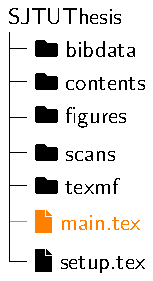
\includegraphics[page=1]{support/figures/thesisdir.pdf}
    \end{column}
    \begin{column}{0.65\textwidth}
      文档类选项是指在载入文档类时的可选选项,多个选项使用逗号隔开,文档类选项会对所有宏包可见。
      \begin{codeblock}[escapechar="]{main.tex}
% !TeX encoding = UTF-8

% 载入 SJTUThesis 模版
"\highlightline"\documentclass[type=master]{sjtuthesis}
% 选项
%   type=[doctor|master|bachelor],
%   zihao=[-4|5],
%   lang=[zh|en],
%   review,
%   [twoside|oneside],
%   math-style=[ISO|TeX],
      \end{codeblock}
    \end{column}
  \end{columns}
\end{frame}

\begin{frame}[fragile]
  \frametitle{文档类选项}
  \begin{columns}
    \begin{column}{0.3\textwidth}
      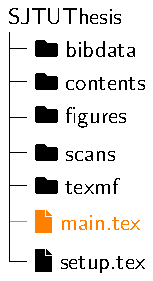
\includegraphics[page=1]{support/figures/thesisdir.pdf}
    \end{column}
    \begin{column}{0.7\textwidth}
      我是学士,写英文论文
      \begin{codeblock}[]{}
|\phantom{}|\documentclass[type=bachelor,lang=en]{sjtuthesis}
      \end{codeblock}
      我是硕士,盲审
      \begin{codeblock}[]{}
|\phantom{}|\documentclass[type=master,review]{sjtuthesis}
      \end{codeblock}
      我是博士,先写着电子版不空页
      \begin{codeblock}[]{}
|\phantom{}|\documentclass[type=doctor,oneside]{sjtuthesis}
      \end{codeblock}
    \end{column}
  \end{columns}
  \note{有 ChatGPT 那味了。}
\end{frame}

\begin{frame}
  \frametitle{文档类选项}
  \begin{columns}
    \begin{column}{0.35\textwidth}
      \includegraphics[page=2,scale=0.9]{support/figures/thesisdir.pdf}
    \end{column}
    \begin{column}{0.65\textwidth}
      \begin{table}
        \caption{文档类选项}
        \footnotesize
        \begin{tabular}{>{\ttfamily}rll}
          \toprule
          选项 & 含义 & 相关 \\
          \midrule
          type= & 指定论文类型 & 第 \ref{covers} 页\\
          \midrule
          cjk-font= & 指定中文字体 & \\
          text-font= & 指定西文字体 & 第 \ref{frame:fonts} 页\\
          math-font= & 指定数学字体 & \\
          math-style= & 指定数学样式 & 第 \ref{frame:math-style} 页\\
          \midrule
          review & 开启盲审模式 & \thesisissue{195} \thesisissue{686} \\
          twoside & 双页模式 & \thesisissue{554} \\
          oneside & 单页模式 & \thesisissue{694} \\
          openright & 章从奇数页开始 & \thesisdiscuss{724} \\
          openany & 章从任意页开始 & \thesisissue{446} \\
          \bottomrule
        \end{tabular}
      \end{table}

      更多文档类选项查阅 \textsc{SJTU\TeX{}} 的开发文档 \link{https://github.com/sjtug/SJTUTeX/releases/download/v1.1.0/sjtuthesis.pdf}。
    \end{column}
  \end{columns}
\end{frame}

\begin{frame}[label={frame:fonts}]
  \frametitle{字体配置}
  \newcommand{\noticemark}{\alert{\normalshape \textopenbullet}}
  \begin{columns}
    \begin{column}{0.35\textwidth}
      \includegraphics[page=3,scale=0.9]{support/figures/thesisdir.pdf}
    \end{column}
    \begin{column}{.65\textwidth}
      相较于 \CTeX{} 使用 \texttt{fontset} 设定中文字体集,
      \SJTUThesis{} 还提供了西文、数学字体集的设定\footnotemark。

      {
        \medskip
        \ttfamily\scriptsize
        \alert{cjk-font=...\hfill 中文字体}
        
        \stamphrule\medskip

        \foreach \sjtufontname/\sjtufontdesc in {adobe/{adobe \faAdobe\noticemark},{fandol}/{fandol \faLinux{} \noticemark},{founder},mac/{mac \faApple{} \noticemark},windows/{windows \faWindows},ubuntu/{ubuntu \noticemark}}{
          \begin{minipage}{2.2cm}
            \centering
            \includefontpreview{support/thesis/cjkfont-\sjtufontname.pdf}\\
            \raisebox{0.8ex}{\sjtufontdesc}
          \end{minipage}
        }

        \bigskip

        \alert{text-font=..., math-font=...\hfill 西文与数学字体}

        \stamphrule\medskip

        \foreach \sjtufontname/\sjtufontdesc in {{cambria}/{cambria \noticemark},{lm},{newcm}/{newcm \noticemark},{newpx},{newtx},{stixtwo}/{stixtwo \noticemark},{times},{xits}/{xits \noticemark}}{
          \begin{minipage}{2cm}
            \centering
            \includefontpreview{support/thesis/latinfont-\sjtufontname.pdf}\\
            \raisebox{0.8ex}{\sjtufontdesc}
          \end{minipage}
        }
      }
    \end{column}
  \end{columns}
  \footnotetext{\noticemark 表示无法使用 pdf\LaTeX{} 编译。}
\end{frame}

\begin{frame}[label={frame:math-style}]
  \frametitle{数学样式}
  \begin{columns}
    \begin{column}{0.35\textwidth}
      \includegraphics[page=2,scale=0.9]{support/figures/thesisdir.pdf}
    \end{column}
    \begin{column}{0.65\textwidth}
      新增数学样式 \texttt{math-style} 文档类选项,现在默认为 \texttt{ISO},
      如果更喜欢原始的 \TeX{} 数学样式,可以切换为 \texttt{TeX}。

      \begin{minipage}[c]{10em}
        \texttt{math-style=ISO}
      \end{minipage}
      \begin{minipage}[c]{5cm}
        \includemathstylepreview{support/thesis/mathstyle-ISO.pdf}
      \end{minipage}
       
      \begin{minipage}[c]{10em}
        \texttt{math-style=TeX}
      \end{minipage}
      \begin{minipage}[c]{5cm}
        \includemathstylepreview{support/thesis/mathstyle-TeX.pdf}
      \end{minipage}

      \begin{block}{}
        请注意在默认情况下(\texttt{math-style=ISO})应当使用 \cmd{increment} 而不是 \cmd{Delta} 表示有限增量。
      \end{block}
    \end{column}
  \end{columns}
\end{frame}

\begin{frame}[fragile]
  \frametitle{基本配置}
  \begin{columns}
    \begin{column}{0.35\textwidth}
      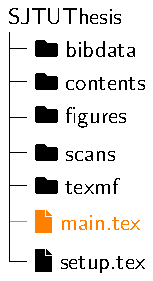
\includegraphics[page=1]{support/figures/thesisdir.pdf}
    \end{column}
    \begin{column}{0.65\textwidth}

      \only<1>{
        在 \texttt{main.tex} 中引入 \texttt{setup.tex} 来导入主要的信息录入与宏包加载配置。
      }

      \only<2>{
        \alert{\textbf{(a,b)}} 其中 \cmd{sjtusetup}(第 \ref{sjtusetup} 页)中的 \opt{info} 将会修改封面的信息设置。
      }

      \begin{codeblock}[firstnumber=12]{main.tex}
|\highlightline<1>|% 论文基本配置,加载宏包等全局配置
|\highlightline<1>|\input{setup}

\begin{document}

%TC:ignore

|\highlightline<2>|% 标题页
|\highlightline<2>|\maketitle
      \end{codeblock}
    \end{column}
  \end{columns}
\end{frame}

\begin{frame}[fragile, label=sjtusetup]
  \frametitle{基本配置}
  \begin{columns}
    \begin{column}{0.35\textwidth}
      \includegraphics[page=4]{support/figures/thesisdir.pdf}
    \end{column}
    \begin{column}{0.65\textwidth}
      \vspace*{-0.2cm}
      \begin{codeblock}[firstnumber=3]{setup.tex}
\sjtusetup{
  info = {
    zh/title  = {|\phantom{}|上海交通大学学位论文 \LaTeX{} 模板示例文档},
    en/title  = {A Sample for \LaTeX-based SJTU Thesis Template},
    zh/author = {|\phantom{}|某\quad{}某},
    en/author = {Mo Mo},
  },
  style = { float-seperator = {--}, },
  name = {
    achv = {|\phantom{}|攻读学位期间完成的论文},
  },
}
      \end{codeblock}
    \end{column}
  \end{columns}
\end{frame}

\begin{frame}[label=setup]
  \frametitle{基本配置}
  \begin{columns}
    \begin{column}{0.35\textwidth}
      \includegraphics[page=4]{support/figures/thesisdir.pdf}
    \end{column}
    \begin{column}{0.65\textwidth}
      \begin{table}
        \centering
        \caption{info 域}
        \footnotesize
        \begin{tabular}{lll} \toprule
          命令作用     & 中文对应选项                      & 英文对应选项                 \\ \midrule
          论文标题     & \texttt{zh/title}                 & \texttt{en/title}            \\
          关键字列表   & \texttt{zh/keywords}              & \texttt{en/keywords*}        \\
          作者姓名     & \texttt{zh/author}                & \texttt{en/author}           \\
          申请学位名称 & \texttt{zh/degree}                & \texttt{en/degree}           \\
          院系名称     & \texttt{zh/department}            & \texttt{en/department}       \\
          专业名称     & \texttt{zh/major}                 & \texttt{en/major}            \\
          导师         & \texttt{zh/supervisor}            & \texttt{en/supervisor}       \\
          副导师       & \texttt{zh/assoc-supervisor}      & \texttt{en/assoc-supervisor} \\
          联培导师     & \texttt{zh/co-supervisor}         & \texttt{en/co-supervisor}    \\
          日期         & \multicolumn{2}{c}{\texttt{date}}                                \\
          学号         & \multicolumn{2}{c}{\texttt{id}}                                  \\ \bottomrule
        \end{tabular}
      \end{table}
    \end{column}
  \end{columns}
  \note{有些选项是 v2 更名或新增的。}
  \note{注意现在使用语言前缀作为键名。}
\end{frame}

\begin{frame}[fragile]
  \frametitle{版权页}
  \begin{columns}
    \begin{column}{0.4\textwidth}
      \includegraphics[page=5]{support/figures/thesisdir.pdf}
    \end{column}
    \begin{column}{0.6\textwidth}
      \alert{\textbf{(c)}} \cmd{copyrightpage} 可以用于插入版权页。
      也可接受一个可选参数,用于直接使用扫描件,此时需要载入 \pkg{pdfpages} 包。\thesisissue{473}

      \begin{codeblock}[firstnumber=22]{main.tex}
% 原创性声明及使用授权书
\copyrightpage
% 插入外置原创性声明及使用授权书
% 导言区添加 \usepackage{pdfpages}
% \copyrightpage[scans/sample-copyright-old.pdf]
      \end{codeblock}
    \end{column}
  \end{columns}
\end{frame}

\begin{frame}[fragile]
  \frametitle{三个部分}
  \framesubtitle{前置部分}
  \begin{columns}
    \begin{column}{0.4\textwidth}
      \includegraphics[page=8]{support/figures/thesisdir.pdf}
    \end{column}
    \begin{column}{0.6\textwidth}
      \alert{\textbf{(d,e,f,g,h)}} 前言从 \cmd{frontmatter} 处开始,页码设置为大写罗马数字,主要包含摘要和目录内容。
      \begin{codeblock}[firstnumber=27]{main.tex}
|\highlightline|% 前置部分
|\highlightline|\frontmatter

% 摘要
\input{contents/abstract}

% 目录
\tableofcontents
% ...
      \end{codeblock}
    \end{column}
  \end{columns}
\end{frame}

\begin{frame}[fragile]
  \frametitle{三个部分}
  \framesubtitle{正文部分}
  \begin{columns}
    \begin{column}{0.4\textwidth}
      \includegraphics[page=9]{support/figures/thesisdir.pdf}
    \end{column}
    \begin{column}{0.6\textwidth}
      \alert{\textbf{(i,j,k)}} 正文从 \cmd{mainmatter} 处开始,页码设置为正常数字,包含正文、参考文献、附录内容。
      \begin{codeblock}[firstnumber=47]{main.tex}
|\highlightline|% 主体部分
|\highlightline|\mainmatter

% 正文内容
\input{contents/intro}
\input{contents/math_and_citations}
\input{contents/floats}
\input{contents/summary}

%TC:ignore

% 参考文献
\printbibliography[heading=bibintoc]

% 附录
\appendix
      \end{codeblock}
    \end{column}
  \end{columns}
\end{frame}

\begin{frame}[fragile]
  \frametitle{三个部分}
  \framesubtitle{结尾部分}
  \begin{columns}
    \begin{column}{0.4\textwidth}
      \includegraphics[page=10]{support/figures/thesisdir.pdf}
    \end{column}
    \begin{column}{0.6\textwidth}
      \alert{\textbf{(k,l,m,n)}} 结尾从 \cmd{backmatter} 处开始,页码设置为正常数字,包含致谢等相关情况。
      \begin{codeblock}[firstnumber=71]{main.tex}
|\highlightline|% 结尾部分
|\highlightline|\backmatter

% 用于盲审的论文需隐去致谢、发表论文、科研成果、简历

% 致谢
\input{contents/acknowledgements}

% 发表论文及科研成果
% 盲审论文中,发表论文及科研成果等仅以第几作者注明即可,不要出现作者或他人姓名
\input{contents/achievements}

%...
      \end{codeblock}
    \end{column}
  \end{columns}
\end{frame}

\begin{frame}
  \frametitle{数学定理环境}
  \begin{columns}
    \begin{column}{0.4\textwidth}
      \includegraphics[page=6]{support/figures/thesisdir.pdf}
    \end{column}
    \begin{column}{0.6\textwidth}
      \SJTUThesis{} 定义了常用的数学环境(需要引入 \pkg{ntheorem} 或者 \pkg{amsthm} 宏包)。

      \begin{table}
        \centering
        \caption{\textsc{SJTUThesis} 定义的数学环境}
        \footnotesize
        \begin{tabular}{>{\ttfamily}rl|>{\ttfamily}rl}
          \toprule
          assumption  & 假设  & lemma       & 引理 \\
          axiom       & 公理  & problem     & 问题 \\
          conjecture  & 猜想  & proof       & 证明 \\
          corollary   & 推论  & proposition & 命题 \\
          definition  & 定义  & remark      & 注   \\
          example     & 例    & solution    & 解   \\
          exercise    & 练习  & theorem     & 定理 \\
          \bottomrule
        \end{tabular}
      \end{table}
    \end{column}
  \end{columns}
\end{frame}

\begin{frame}[fragile]
  \frametitle{参考文献}
  \begin{columns}
    \begin{column}{0.4\textwidth}
      \includegraphics[page=7]{support/figures/thesisdir.pdf}
    \end{column}
    \begin{column}{0.6\textwidth}
      \begin{codeblock}[firstnumber=111,numbersep=2pt]{setup.tex}
% 使用 BibLaTeX 处理参考文献
%   biblatex-gb7714-2015 常用选项
%     gbnamefmt=lowercase     姓名大小写由输入信息确定
%     gbpub=false             禁用出版信息缺失处理
\usepackage[backend=biber,style=gb7714-2015]{biblatex}
% 文献表字体
% \renewcommand{\bibfont}{\zihao{-5}}
% 文献表条目间的间距
\setlength{\bibitemsep}{0pt}
|\highlightline|% 导入参考文献数据库
|\highlightline|\addbibresource{bibdata/thesis.bib}
      \end{codeblock}
    \end{column}
  \end{columns}
\end{frame}

\begin{frame}
  \frametitle{Word}
  \begin{itemize}
    \item[{\faQuestionCircle[regular]}] 跟 Word 的参考实现略有不同 
    \item[{\faCheckCircle[regular]}] 毕设论文的格式只要不违背《上海交通大学关于本科生毕业设计(论文)工作的指导意见》\link{https://github.com/sjtug/SJTUThesis/files/6505296/default.pdf} \thesisissue{621}、《上海交通大学博士、硕士学位论文撰写指南》\link{https://www.gs.sjtu.edu.cn/info/1143/5801.htm} \thesisissue{652} 即可,其他细节上的修改可以先搜索解决方案,再反馈给我们。
    \item[{\faQuestionCircle[regular]}] 我需要转为 Word 文档
    \item[{\faCheckCircle[regular]}] PDF 转为 Word 文档属于逆向工程,暂时不存在完全正确的转换方法 \link{https://www.bilibili.com/video/BV1Vi4y1C71M},从 \LaTeX{} 源代码出发的转换可以使用其他工具实现 \thesisissue{480} \thesisissue{500}。
  \end{itemize}
\end{frame}

\begin{frame}
  \frametitle{还有其他问题?}
  % \begin{columns}
    % \begin{column}{0.73\textwidth}
      \begin{itemize}
        \item[{\faComment*[regular]}] 日常模板或 \LaTeX{} 使用问题可以前往 Discussions \link{https://github.com/sjtug/SJTUThesis/discussions} 提问

        (解决后别忘了 \textcolor{green}{\faCheckCircle{} Mark as answer}
        \item[{\faDotCircle[regular]}] 如果是 \textsc{SJTUThesis} 项目本身的 bug 和 feature request

        可以通过 Issues \link{https://github.com/sjtug/SJTUThesis/issues} 反馈。
        \item[{\faCodeBranch}] 如果你有好点子,可以贡献代码

          向 \textsc{SJTU\TeX{}} \link{https://github.com/sjtug/SJTUTeX} 存储库发 PR,\par
          而后把解包结果同步到 \textsc{SJTUThesis}。
        
        \item[{\faQq}] 也欢迎在 QQ 群(715273806)即时讨论。
        \note{群之前满了,社长给腾讯充了钱,让它可以接着塞人。}
      \end{itemize}
    % \end{column}
    % \begin{column}{0.27\textwidth}
    %   \includegraphics[height=0.7\textheight]{support/images/qq.jpg}
    % \end{column}
  % \end{columns}
\end{frame}

\end{document}
      \end{codeblock}
    \end{column}
  \end{columns}
  \footnotetext{如果想强制指定子文档的主文档,可以在文件第一行输入魔术命令:\texttt{\% !TeX root = main.tex}}
\end{frame}

\section{图}
\begin{frame}[fragile]%
  \frametitle{\temporal<5>{插图}{浮动体}{插图}}
  \begin{columns}
    \begin{column}{0.6\textwidth}
      \begin{codeblock}[]{插入单图\only<4->{最佳实践}}
\documentclass{ctexart}
|\highlightline<2>|\usepackage{graphicx}
|\highlightline<2>|\graphicspath{{figs/}{pics/}}
\begin{document}
|\highlightline<5>|\begin{figure}[ht]
|\highlightline<6>|  \centering
|\highlightline<3>|  \includegraphics[width=|\only<1-3>{4cm}\only<4->{0.4\textbackslash{}textwidth}|]{sjtug}
|\highlightline<7>|  \caption{SJTUG 徽标}\label{fig:sjtug}
|\highlightline<5>|\end{figure}
\end{document}
      \end{codeblock}
    \end{column}
    \begin{column}{0.4\textwidth}
      \only<1>{
        \includepdflarge{support/examples/insertimage.pdf}
      }

      \only<2>{
        为了插入外部图片,需要使用 \pkg{graphicx} 宏包。之后在文档主体便可以使用 \cmd{includegraphics} 插入图片。导言区也可以加入 \cmd{graphicspath} 指定图片文件夹\footnotemark。
      }

      \only<3>{
        \cmd{includegraphics} 命令便以相对路径的方式插入图片,如果无同名图片,那么后缀名可以省略。可以使用可选参数指定插入的图片尺寸,最佳实践是使用 \cmd{textwidth} 或 \cmd{linewidth} 的相对值指定尺寸大小,以在未来可能的布局更改中保留一定的灵活性。
        \note{比如我未来想变更为幻灯片的时候。}
      }

      \only<4>{
        也可以通过键值对的方法设置图片的其他属性。
        \note{事实上,\LaTeX{} 很多命令都是使用方括号添加可选参数的。}
        \begin{center}
          \footnotesize
          \begin{tabular}{rl}
            \opt{width} & 宽度 \\
            \opt{height} & 高度 \\
            \opt{scale} & 缩放 \\
            \opt{angle} & 角度 \\
          \end{tabular}
        \end{center}
      }

      \only<5>{
        \env{figure} 为一个浮动体环境(\env{table} 也是),可以将其移动到其他位置上以减少行文中的空白。可以添加可选参数以指定如何放置浮动体,最多可以使用四种位置描述符:
        \begin{center}
          \footnotesize
          \begin{tabular}{cll}
            \opt{h} & Here & 尽可能在这里 \\
            \opt{t} & Top & 页面顶部 \\
            \opt{b} & Bottom & 页面底部 \\
            \opt{p} & Page & 浮动体专页 \\
          \end{tabular}
        \end{center}
        还可以只使用 \pkg{float} 宏包提供的 \opt{H} 描述符以强制置于此处。
      }

      \only<6>{
        采用 \cmd{centering} 命令而不是 \env{center} 环境来水平居中图片。这将避免多余的纵向间距。
      }

      \only<7>{
        使用 \cmd{caption} 命令输入题注,如果这个命令写在插入图片前面,题注将会在上方(中文中一般对 \env{table} 环境这么做)。后面将会看到如何对留有标记(\cmd{label})的图片进行引用。
      }
    \end{column}
  \end{columns}
  \only<2>{\footnotetext{其命令参数每个为一个以 \texttt{/} 结尾的文件夹,每个文件夹需要使用大括号包裹起来。}}
\end{frame}

\begin{frame}[fragile]
  \begin{columns}
    \begin{column}{0.6\textwidth}
      \begin{codeblock}[]{插入双图}
\documentclass{ctexart}
\usepackage{graphicx}
\graphicspath{{figs/}{pics/}}
\begin{document}
  \begin{figure}[ht]
|\highlightline<1>|    \begin{minipage}{0.48\textwidth}
      \centering
      \includegraphics[height=2cm]{sjtug}
|\highlightline<2>|      \caption{SJTUG 徽标}\label{fig:sjtug}
|\highlightline<1>|    \end{minipage}\hfill
|\highlightline<1>|    \begin{minipage}{0.48\textwidth}
      \centering
      \includegraphics[height=2cm]{sjtugt}
|\highlightline<2>|      \caption{SJTUG|\phantom{}|文字}\label{fig:sjtugt}
|\highlightline<1>|    \end{minipage}
  \end{figure}
\end{document}
      \end{codeblock}
    \end{column}
    \begin{column}{0.4\textwidth}

      \only<1>{
        在 \env{figure} 环境里使用 \env{minipage} 小页制作列盒子,以并排两图并分别编号,需要设定强制参数以指定列宽。两个小页之间添加 \cmd{hfill} 使两个小页两端对齐。
      }

      \only<2>{
        在每个小页内部分别使用 \cmd{caption} 添加标签。
      }

      \only<3>{
        \includepdflarge{support/examples/doubleimages.pdf}
      }
    \end{column}
  \end{columns}
\end{frame}

\begin{frame}[fragile]%
  \begin{columns}
    \begin{column}{0.6\textwidth}
      \begin{codeblock}[]{}
\documentclass{ctexart}
\usepackage{graphicx}
|\highlightline|\usepackage{subcaption}
\graphicspath{{figs/}{pics/}}
\begin{document}
  \begin{figure}[ht]
|\highlightline|    \begin{subfigure}{0.48\textwidth}
      \centering
      \includegraphics[height=2cm]{sjtug}
      \caption{|\phantom{}|徽标}
|\highlightline|    \end{subfigure}\hfill
|\highlightline|    \begin{subfigure}{0.48\textwidth}
      \centering
      \includegraphics[height=2cm]{sjtugt}
      \caption{|\phantom{}|文字}
|\highlightline|    \end{subfigure}
    \caption{SJTUG}\label{fig:sjtug}
  \end{figure}
\end{document}
      \end{codeblock}
    \end{column}
    \begin{column}{0.4\textwidth}
      \includepdflarge{support/examples/subfigures.pdf}\vspace{15pt}
      \pkg{subcaption} 宏包提供了 \env{subfigure} 环境(以及 \env{subtable}),可以用于以子图的形式插入,编号会增加一级。也可以为子图添加子级引用编号。
    \end{column}
  \end{columns}
\end{frame}

\section{表}
\begin{frame}[fragile]
  \frametitle{简单表格}
  \begin{columns}
    \begin{column}{0.6\textwidth}
      \begin{codeblock}[]{}
\documentclass{ctexart}
|\only<1-2>{\highlightline}|\usepackage{|\temporal<1>{array}{\highlight{array}}{array},\temporal<2>{booktabs}{\highlight{booktabs}}{booktabs}|}
\begin{document}
\begin{table}[ht]
  \centering
  \caption{|\phantom{}|北京冬奥会吉祥物}
|\highlightline<1>|  \begin{tabular}{lp{3cm}}
|\highlightline<2>|    \toprule
|\highlightline<3>|吉祥物 & 描述                          \\
|\highlightline<2>|    \midrule
|\highlightline<3>|冰墩墩 & 2022 年北京冬季奥运会吉祥物  \\
|\highlightline<3>|雪容融 & 2022 年北京冬季残奥会吉祥物  \\
|\highlightline<2>|    \bottomrule
|\highlightline<1>|  \end{tabular}
\end{table}
\end{document}
      \end{codeblock}
    \end{column}
    \begin{column}{0.4\textwidth}
      
      \only<1>{
        使用 \env{tabular} 环境绘制表格。需要添加参数(称为\textbf{表格导言})以确定每一列的对齐方式。引入 \pkg{array} 宏包来使用更多的\textbf{引导符}。
        \begin{center}
          \footnotesize
          \begin{tabular}{>{\ttfamily}ll}
            \alert{l} & 向左对齐 \\
            \alert{c} & 居中对齐 \\
            \alert{r} & 向右对齐 \\
            \alert{p\{3cm\}} & 固定列宽,两端对齐 \\
            \alert{m\{3cm\}} & \texttt{p} + 垂直居中对齐 \\
            \alert{>\{\textbackslash{}bfseries\}} & 后一列单元格前加命令 \\
            \alert{*\{3\}\{l\}} & 三个左对齐列 \\
          \end{tabular}
        \end{center}
      }

      \only<2>{
        \pkg{booktabs} 宏包提供了标准三线表格所需要的行分割线:\cmd{toprule},\cmd{midrule},\cmd{bottomrule}。也可以使用 \cmd{cmidrule\{1-2\}} 来部分地绘制行分割线。一般不推荐在专业表格中使用纵向分割线。
      }

      \only<3>{
        每行内容使用 \textbackslash\textbackslash{} 分隔开,每行中的单元格使用 \& 分隔开。
      }

      \only<4>{
        \includepdflarge{support/examples/table.pdf}
      }
    \end{column}
  \end{columns}
\end{frame}

\begin{frame}[fragile]%
  \begin{columns}
    \begin{column}{0.6\textwidth}
      \begin{codeblock}[]{表头居中}
\documentclass{ctexart}
\usepackage{array,booktabs}
\begin{document}
\begin{table}[ht]
  \centering
  \caption{|\phantom{}|北京冬奥会吉祥物}
  \begin{tabular}{lp{3cm}}
    \toprule
|\highlightline|\multicolumn{1}{c}{|\phantom{}|吉祥物} &
|\highlightline|\multicolumn{1}{c}{|\phantom{}|描述} \\
    \midrule
|\phantom{}|冰墩墩 & 2022 年北京冬季奥运会吉祥物  \\
|\phantom{}|雪容融 & 2022 年北京冬季残奥会吉祥物  \\
    \bottomrule
  \end{tabular}
\end{table}
\end{document}
      \end{codeblock}
    \end{column}
    \begin{column}{0.4\textwidth}
      \cmd{multicolumn} 命令不仅可以用于合并同行的单元格,还可以用于临时地屏蔽表格导言对该列的对齐方式定义。这里用于居中表头。
      \begin{center}
        \parbox{0.85\linewidth}{
          \cmd{multicolumn\{格数\}\{对齐方式\}\{内容\}}
        }
      \end{center}
      跨页表格考虑使用 \pkg{longtable} 宏包。带标注的表格可以考虑使用 \pkg{threeparttable} 宏包。考虑使用在线工具生成表格代码 \link{https://www.tablesgenerator.com/latex_tables}。
      \note{复杂的使用方法在 \SJTUThesis{} 示例文档中都有提及。}
    \end{column}
  \end{columns}
\end{frame}

\section{数学公式}
\begin{frame}
  \frametitle{数学模式}
  \begin{alertblock}{}
  输入数学公式是 \LaTeX{} 的绝对强项,很多常见的公式服务依赖于一些轻量级渲染引擎比如 MathJax, K\kern-.3ex\raise.4ex\hbox{\footnotesize A}\kern-.3ex\TeX{}。但是它们实际上使用的是 \LaTeX{} 语法变种,也就是说并没有使用 \LaTeX{} 后端。所以不要期望有完全一致的输出。
  \end{alertblock}
  
  为了更好的获得数学公式输入支持,请使用 \hologo{AmS}math 宏包。数学模式分为两种:
  \begin{description}
    \item[行内模式] 一般通过一对美元符号(\$$\cdots$\$)标记,可以使用编辑器内建的符号表输入数学符号,也可以使用在线工具手写识别 \link{https://detexify.kirelabs.org/classify.html}。
    \item[行间模式] 一般通过 \env{equation} 环境\footnote{这是有编号环境,其加星号的变种 \env{equation*} 用于生成无编号环境。}输入。如果需要使用多行公式,请使用 \env{align} 环境,并按照类似表格输入的方式,使用 \& 对齐符号,\textbackslash\textbackslash{} 换行。如果不想手动居中,可以考虑多行自动居中的 \env{gather} 和单个大型公式首尾两端对齐 \env{multline}。
  \end{description}
  \note{关于表格和数学公式,如果不太熟悉如何输入,或者符号表记不住,推荐从比较容易上手的编辑器起步,比如 \TeX{}studio 提供了用户友好的界面(\faWindows{} 上的向导 $\rightarrow$ 数学助手)。我相信输入半年后,就可以对这些符号的输入很熟练了。
  
  你会发现我的这套教程没有讲很多的数学公式输入技巧,因为这些东西只有你自己熟练了才能体会。而且 \LaTeX{} 本来就不是完全关于数学公式的。}
\end{frame}

\begin{frame}
  \frametitle{数学命令展示}
  \begin{columns}
    \begin{column}{0.33\textwidth}
      \begin{exampleblock}{}
        $PV=nRT$
      \end{exampleblock}
      \begin{exampleblock}{}
        $\sum_{i=1}^ki^2=\frac{n(n+1)(2n+1)}{6}$
      \end{exampleblock}
      \begin{exampleblock}{}
        $T(n) = aT\left(\left\lceil\frac{n}{b}\right\rceil\right) + \mathcal{O}(n^d)$
      \end{exampleblock}
      \begin{exampleblock}{}
        $\frac{x_{1}+x_{2}+x_{3}}{3}\geq \sqrt[3]{x_{1}x_{2}x_{3}}$
      \end{exampleblock}
      \begin{exampleblock}{}
        $n=(\underbrace{1\cdots 1}_{k\text{ of 1's}})_2=2^{k+1}-1$
      \end{exampleblock}
      \begin{exampleblock}{}
        $\nabla f (P)= \left.\left(\frac{\partial f}{\partial x},\frac{\partial f}{\partial y},\frac{\partial f}{\partial z}\right)\right|_{P}$
      \end{exampleblock}
    \end{column}
    \begin{column}{0.67\textwidth}
      \begin{exampleblock}{}
        \begin{equation*}
          \int_{a}^b f(x)\,\mathrm{d}x=\lim_{|P|\rightarrow 0}\sum_{i=1}^n f(\xi_i)\Delta x_i
        \end{equation*}
      \end{exampleblock}
      \begin{exampleblock}{}
        \begin{equation}
          T(n) = \begin{cases}
            \mathcal{O}(n^d),&\textrm{if } d>\log_b a, \\
            \mathcal{O}(n^d\log n), &\textrm{if } d=\log_b a,\\
            \mathcal{O}(n^{\log_b a}), &\textrm{if } d<\log_b a.
          \end{cases}
        \end{equation}
      \end{exampleblock}
      \begin{exampleblock}{}
        \begin{align}
          Q^{T}A&=R \\
          \begin{pmatrix}
            q_1^T \\ q_2^T \\ q_3^T
          \end{pmatrix}
          \begin{pmatrix}
            a_1 & a_2 & a_3
          \end{pmatrix}
          &=R
        \end{align}
      \end{exampleblock}
    \end{column}
  \end{columns}
  \note{关于如果 \LaTeX{} 报出了错误,比如说数学模式下不能有空行,想要学习如何修复这些错误,
  可以详见 Learn\LaTeX{}.org 的相关章节
  \link{https://github.com/CTeX-org/learnlatex.github.io/blob/zh-Hans/zh-Hans/lesson-15.md}。}
\end{frame}

%更深入地讲解 mathtools, unicode-math, siunix

\section{引用}
\begin{frame}[fragile]
  \frametitle{交叉引用}
  \only<1>{
    正如之前所提到的,\LaTeX{} 中使用 \cmd{label} 标记,然后可以使用 \cmd{ref} 来引用这个标记。 \cmd{label} 可以放在使用计数器的对象之后。
  }

  \only<2>{
    为了使得对公式编号的引用带有括号,推荐使用 \hologo{AmS}math 宏包中的 \cmd{eqref} 命令。对于多行公式环境,每一个换行符前都可以添加一个 \cmd{label} 用于引用该行公式。
  }
  
  \begin{columns}
    \begin{column}{0.5\textwidth}
      \begin{codeblock}[]{图}
\begin{figure}
|\highlightline<1>|  \caption{|\phantom{}|示例}\label{fig:example}
\end{figure}
      \end{codeblock}
      \begin{codeblock}[]{表}
\begin{table}
|\highlightline<1>|  \caption{|\phantom{}|示例}\label{tab:example}
\end{table}
      \end{codeblock}
    \end{column}
    \begin{column}{0.5\textwidth}
\begin{codeblock}[]{目次}
|\highlightline<1>|\section{|\phantom{}|示例}\label{sec:example}
\end{codeblock}

\begin{codeblock}[]{公式}
\begin{equation}
  a = b + c
|\highlightline<1>|\label{eq:example}
\end{equation}
|\highlightline<2>|如公式 \eqref{eq:example} 所示,
\end{codeblock}
    \end{column}
  \end{columns}
\end{frame}

\begin{frame}[fragile]
  \frametitle{文献引用}
  \LaTeX{} 可以通过专用数据库文件 \texttt{.bib} 自动生成参考文献,很多的文献管理文件比如 EndNote \link{https://lic.sjtu.edu.cn/Default/softshow/tag/MDAwMDAwMDAwMLGImKE}, Zotero \link{https://www.zotero.org/}, JabRef \link{https://www.jabref.org/} 都可以直接导出这种格式的文件用于 \LaTeX{} 论文中的引用。一般不需要手写数据库文件,你只需要注意每一个文献会在数据库中有一个主键,这个类似于上文的 \cmd{label} 标记,只是要引用数据库中的文献需要使用 \cmd{cite} 命令。
  
  \begin{codeblock}[]{ref.bib}
|\highlightline|@article{devoftech,|\hfill\alert{\% 类型为期刊论文,主键为\texttt{devoftech}}|
  title={|\phantom{}|新时期我国信息技术产业的发展},
  author={|\phantom{}|江泽民},
  year={2008}
}
  \end{codeblock}
\end{frame}

\begin{frame}
  \frametitle{文献引用}
  而让 \LaTeX{} 处理 \texttt{.bib} 数据库文件与引用有两种工作流。你可能需要查清楚如何在编辑器中设置对应的工作流,或者采用后面所提到的高级编译方式 \texttt{latexmk}。
  \begin{columns}
    \begin{column}{0.5\textwidth}
      \begin{block}{\hologo{BibTeX} + \pkg{natbib}}
        一般期刊提交使用这种方法,\pkg{natbib} 宏包将提供命令 \cmd{citet}(文本引用) 和 \cmd{citep}(括号引用)。
      \end{block}
      \begin{alertblock}{\hologo{BibTeX} + \pkg{gbt7714}}
        中文引用可以直接使用 \pkg{gbt7714} 宏包,但是角模式和正文模式不能混用。
      \end{alertblock}
    \end{column}
    \begin{column}{0.5\textwidth}
      \begin{block}{\hologo{biber} + \pkg{biblatex}}
        这是更容易自定义的方法,与 \hologo{BibTeX} 的运作方式稍有不同。\pkg{biblatex} 提供了更加智能的引用命令。
      \end{block}
      \begin{alertblock}{\hologo{biber} + \pkg{biblatex-gb7714-2015}}
        而中文引用可以使用 \pkg{biblatex} 宏包的样式 \pkg{gb7714-2015}。
      \end{alertblock}
    \end{column}
  \end{columns}
\end{frame}

\begin{frame}[fragile]
  \frametitle{文献引用}
  \begin{columns}
    \begin{column}{0.5\textwidth}
      \begin{codeblock}[]{\hologo{BibTeX} + \pkg{gbt7714}}
\documentclass{ctexart}
\usepackage{gbt7714}
\bibliographystyle{gbt7714-numerial}
% \citestyle{numbers}  % 正文模式
\begin{document}
  |\phantom{}|他指出了...\cite{devoftech}
  \bibliography{ref}
\end{document}
      \end{codeblock}
    \end{column}
    \begin{column}{0.5\textwidth}
      \begin{codeblock}[]{\hologo{biber} + \pkg{biblatex-gb7714-2015}}
\documentclass{ctexart}
\usepackage[backend=biber,style=gb7714-2015]{biblatex}
\addbibresource{ref.bib}
\begin{document}
  |\phantom{}|他在文献 \parencite{devoftech}
  |\phantom{}|指出了...\cite{devoftech}
  \printbibliography
\end{document}
      \end{codeblock}
    \end{column}
  \end{columns}
\end{frame}

\begin{frame}
  \frametitle{文献引用}
  \begin{columns}
    \begin{column}{0.5\textwidth}
      \includepdflarge{support/examples/bibtex.pdf}
    \end{column}
    \begin{column}{0.5\textwidth}
      \includepdflarge{support/examples/biblatex.pdf}
    \end{column}
  \end{columns}
  \note{这页有一篇上过《新闻联播》的论文。}
\end{frame}

\end{shadedsection}

|\highlightline<3>|  % !TeX root = ../../latex-talk.tex

\part{SJTUThesis}

\begin{frame}
  \frametitle{本部分主要参考}
  \begin{bibliolist}{00}
    \onlineitem \textsc{SJTUG}.
    \newblock \textsc{SJTUThesis} 示例文档[EB/OL].
    \newblock 2022. \url{https://github.com/sjtug/SJTUThesis}.

    \onlineitem \textsc{SJTUG}.
    \newblock \textsc{SJTUThesis} 用户文档[EB/OL].
    \newblock 2022. \url{https://github.com/sjtug/SJTUTeX}.
  \end{bibliolist}
\end{frame}

\begin{frame}
  \frametitle{简介}
  \begin{columns}
    \begin{column}{0.6\textwidth}
      \begin{itemize}
        \item 最早由韦建文于 2009 年 11 月发布 0.1a 版
        \item 2018 年起由 SJTUG 接手维护
        \item 2019 年 6 月吴伟健重构了整个宏包的代码,升级版本号为 1.0
        \item 2022 年 11 月模板改版后,吴伟健、张驰等人使用 \LaTeX3 重构 2.0 版本
        \item 最新版:\SJTUThesisVersion{} (\SJTUThesisDate)
        \item 支持本科、硕士、博士学位论文的排版
        \item 推荐使用最新版本的 \TeX{} 发行版编译
      \end{itemize}
    \end{column}
    \begin{column}{0.4\textwidth}
      \begin{exampleblock}{}
        \begin{minipage}[c]{1cm}
          \includegraphics[width=0.8cm]{\getcontribpath{sjtug}{vi/sjtug}}
        \end{minipage}
        \begin{minipage}[c]{3cm}
          \href{https://github.com/sjtug}{sjtug}/\href{https://github.com/sjtug/SJTUThesis}{SJTUThesis}
        \end{minipage}
      \end{exampleblock}
      \vspace{-8pt}
      \begin{block}{}
        \scriptsize
        上海交通大学 \hologo{XeLaTeX} 学位论文及课程论文模板 | Shanghai Jiao Tong University \hologo{XeLaTeX} Thesis Template
      \end{block}
      \vspace{-8pt}
      \begin{alertblock}{}
        \scriptsize
        \begin{tabular}{cl}
          \faStar & 2.6k \\
          \faEye & 52 \\
          \faCodeBranch & 726 \\
        \end{tabular}
      \end{alertblock}
    \end{column}
  \end{columns}
\end{frame}

\begin{frame}
  \frametitle{\only<1>{为什么使用 \LaTeX{} 排版论文?}\only<2>{当然它们也互相学习}}
  \begin{columns}[t]
    \begin{column}{0.25\textwidth}
      \begin{exampleblock}{\faMarkdown{} Markdown}
        \begin{itemize}
          \item[\faPlus] 技术文档流行
          \item[\faPlus] 语法简单 
          \item[\faMinus] 不内置格式控制
        \end{itemize}
      \end{exampleblock}
      \only<2>{
        \begin{block}{}
          \begin{itemize}
            \item[\faBolt] R Markdown (Bookdown) 模板 \link{https://github.com/bubifengyun/SJTUThesis-Rmd} \link{https://github.com/bubifengyun/SJTUThesis-Rmd}
            \item[\faAsterisk] 配套 MathJax 渲染公式  
          \end{itemize}
        \end{block}
      }
    \end{column}
    \begin{column}{0.25\textwidth}
      \begin{exampleblock}{\faFileWord{} Word}
        \begin{itemize}
          \item[\faPlus] 通用论文格式
          \item[\faPlus] 所见即所得
          \item[\faMinus] 进阶排版仍困难 
        \end{itemize}
      \end{exampleblock}
      \only<2>{
        \begin{block}{}
          \begin{itemize}
            \item[\faBolt] 数学公式可以直接通过 \LaTeX{} 格式转换
            \item[\faAsterisk] 也就是 Unicode Math 输入方式 
          \end{itemize}
        \end{block}
      }
    \end{column}
    \begin{column}{0.25\textwidth}
      \begin{block}{\LaTeX{} SJTUThesis}
        \begin{itemize}
          \item[\faPlus] 学术论文格式
          \item[\faPlus] 内容样式分离
          \item[\faMinus] 上手有门槛 
        \end{itemize}
      \end{block}
      \only<2>{
        \begin{exampleblock}{}
          \begin{itemize}
            \item[\faBolt] \TeX{} 的可视前端 \hologo{LyX} \link{https://www.lyx.org/Download} Overleaf Rich Text 模式
            \item[\faAsterisk] \TeX{} 的可视改良 \TeX{}\raise-0.25em\hbox{\footnotesize MACS} \link{http://texmacs.org/tmweb/home/welcome.en.html} \link{https://mogan.app}
          \end{itemize}
        \end{exampleblock}
      }
    \end{column}
    \begin{column}{0.25\textwidth}
      \begin{exampleblock}{\faAdobe{} InDesign}
        \begin{itemize}
          \item[\faPlus] 专业杂志排版
          \item[\faPlus] 精细调整
          \item[\faMinus] 过于繁琐专业  
        \end{itemize}
      \end{exampleblock}
      \only<2>{
        \begin{block}{}
          \begin{itemize}
            \item[\faBolt] 传说用了 \TeX{} 的一些算法 \link{https://mp.weixin.qq.com/s/GASGHK-GsIg2Fwb2jWwpvw}
          \end{itemize}
        \end{block}
      }
    \end{column}
  \end{columns}
  \note{\emph{这页仅作简要介绍。}

  让我们来讨论 the elephant in the room:为什么用 \LaTeX{} 排版论文?
  }
  \note<1>[item]{Markdown 很好啊,方便的语法,一般技术文档也常用。但就是因为它太简单了,没有内置样式控制,一般需要借助 HTML,CSS 那一套东西。}
  \note<2>[item]{也会有一些人尝试通过 R Markdown(Bookdown)改进,当然你也可以试着使用 \LaTeX{} 里的 \pkg{markdown} 宏包
  (这有点像各种前端博客框架渲染 Markdown 为 HTML,只不过这里渲染 \LaTeX{} 生成 PDF,代码抄录方面已经有 Sphinx 这个工具 \link{https://github.com/sphinx-doc/sphinx}),
  以及可以通过 MathJax 渲染 \TeX{} 公式。
  }
  \note<1>[item]{Word 很好啊,官方钦定的论文写作方法,可见即可得,但是进阶排版仍然可以困难。就拿排版公式来说,
  大家以前初高中学的、或者是计算机二级考的 Word 2003 要排版公式,一种是装 MathType 插件,版本间不兼容、一种是搞个域代码+替换字体。}
  \note<2>[item]{Word 2007 之后添加了插入正经的 Unicode 公式功能,但默认的 Calibri Math 字体以及符号布局仍然赶不上 \TeX{} 的美感。
  }
  \note<1>[item]{根据之前学到的一些技巧,看起来不难对吧(虽然有我诱导的成分),然后它内容与样式分离的设计理念已经渗入了很多领域。以及很多学术论文都需要 \LaTeX{} 的提交。}
  \note<2>[item]{当然现在也推出了可见即可得的编辑器 \hologo{LyX},Overelaf 的可视模式(虽然这两个并不是一个东西);以及迟先生很喜欢的 TeXmacs,一种不使用 \TeX{} 底层的、但是效果相像的排版程序。
  }
  \note<1>[item]{设计相关专业的同学可能更喜欢 Adobe Indesign,对图文混排更为擅长。但是它也足够复杂,虽然提供了几乎所有的排版用具,但是我还没见过用它排版几十页充满公式的论文的(或许有人会开先河?)。}
  \note<2>[item]{以及传说它用了 \TeX{} 的一些算法,所以 \TeX{} 还是老大哥,兼具美感和批量化处理的折中方法。}
\end{frame}

\begin{frame}
  \frametitle{开始使用}
  \alert{下载} 推荐安装 Git \link{https://git-scm.com/} 后,克隆 SJTUG 镜像仓库
  \begin{exampleblock}{\faGit*}
    \ttfamily\small
    git clone https://mirror.sjtu.edu.cn/git/SJTUThesis.git/
  \end{exampleblock}

  \alert{编译} 推荐使用 \pkg{latexmk} 编译\footnote{\hologo{MiKTeX} 用户需要手动安装 Perl 解释器 \link{https://www.perl.org/get.html} 才能使用 \pkg{latexmk}。},在不能够利用自带的 \texttt{.latexmkrc} 配置文件的情况下,需要查清楚在对应的编辑器中如何使用 \hologo{XeLaTeX} + \hologo{biber} 编译\footnote{这种情况下,你可能需要查清楚如何全局安装该文档类,并刷新文件名数据库。} \link{https://github.com/sjtug/SJTUThesis/blob/master/README.md}。
  \begin{exampleblock}{\faTerminal}
    \ttfamily\small
    latexmk -xelatex main
  \end{exampleblock}

  \alert{在线} 直接使用 Overleaf 链接 \link{https://www.overleaf.com/latex/templates/sjtuthesis-latex-thesis-template-for-shanghai-jiao-tong-university/mkdwbyjbtfgg?r=sdkbtJ4qGS8kDZQQ&rm=d&rs=b}。
  其他在线平台用户可以下载压缩包,上传至对应平台并采用 \hologo{XeLaTeX} 编译,请注意使用最新版本的 \TeX{} Live。
  \note{不会 Git 的同学可以直接 Download ZIP。}
\end{frame}

\begin{frame}
  \frametitle{手动编译}
  \alert{第一次编译失败} 如果没有办法通过通常方式编译成功,请尝试使用文件夹内附带 \faLinux{}\,\faApple{} \texttt{Makefile} 和 \faWindows{} \texttt{Compile.bat} 进行编译。

  \alert{统计字数} 编写过程中也可以使用对应的命令调用 \TeX{}count 来统计正文字数。
  \begin{columns}
    \begin{column}{0.38\textwidth}
      \begin{exampleblock}{\faLinux{}\,\faApple}
        \ttfamily
        make all\\
        make clean\\
        make cleanall\\
        make wordcount
      \end{exampleblock}
    \end{column}
    \begin{column}{0.38\textwidth}
      \begin{exampleblock}{\faWindows}
        \ttfamily
        ./Compile.bat thesis\\
        ./Compile.bat clean\\
        ./Compile.bat cleanall\\
        ./Compile.bat wordcount
      \end{exampleblock}
    \end{column}
    \begin{column}{0.24\textwidth}
      \begin{block}{\faInfo}
        \ttfamily
        编译论文\\
        清理中间文件\\
        $\hookrightarrow +$删除论文\\
        统计字数
      \end{block}
    \end{column}
  \end{columns}
\end{frame}

\begin{frame}[label=compile]
  \frametitle{编译问题排查}
  \begin{columns}
    \begin{column}{0.33\textwidth}
      \begin{alertblock}{无法使用 \texttt{latexmk}\thesisissue{578}}
        \hologo{MiKTeX} 需要安装 Perl 解释器。
      \end{alertblock}  
      \begin{alertblock}{\CTeX{} 套装无法编译\thesisissue{446}}
        使用最新 \TeX{} 发行版。\link{https://github.com/Aloft-Lab/CTeX-Installer}
      \end{alertblock}
      \begin{alertblock}{\hologo{pdfLaTeX} 无法编译\thesisissue{444}}
        请使用 \texttt{latexmk},或更改编辑器设置以 \hologo{XeLaTeX} 编译。
      \end{alertblock}
    \end{column}
    \begin{column}{0.33\textwidth}
      \begin{alertblock}{缺少字体\thesisissue{564} \thesisdiscuss{598}}
        更换字体集,或者安装对应字体。
      \end{alertblock}
      \begin{alertblock}{缺少汉字\thesisissue{533} \thesisdiscuss{617}}
        去除使用 fandol 字体集的设定。或者是安装字体后,改用 \texttt{cjk-font=adobe} 或 \texttt{cjk-font=founder}。
      \end{alertblock}
    \end{column}
    \begin{column}{0.33\textwidth}
      \begin{block}{\faInfoCircle{} README}
        不同编辑器的设置请首先参阅 README \link{https://github.com/sjtug/SJTUThesis/blob/master/README.md} 文档。
      \end{block}
      \begin{block}{\faBookOpen{} Wiki}
        其他编译问题推荐查阅 Wiki \link{https://github.com/sjtug/SJTUThesis/wiki} 的使用说明部分。
      \end{block}
    \end{column}
  \end{columns}
  \note{两个进阶问题:
  
  如果之前出现了编译错误,在重新编译前,最好清理一下临时文件(\texttt{make clean})。

  如果是 biber 出现了问题,还可以尝试 \texttt{rm -rfv \$(biber --cache)}。\thesisdiscuss{774}
  }
\end{frame}

\begin{frame}[label=covers]
  \frametitle{论文组成}
  \begin{figure}[h]
    \centering
    \foreach \thesispage/\thesisnote in {
      1/{中文封面},3/{英文封面},5/{版权页},7/{中文摘要},9/{英文摘要},11/{目录},13/{插图目录},15/{表格目录},
      17/{正文},27/{参考文献},29/{附录},31/{成果},33/{致谢},35/{大摘要}} {%
      \begin{subfigure}{.13\textwidth}
        \centering
        \fzerobox{\includegraphics[width=\textwidth,page=\thesispage]{support/thesis/sample-thesis-zh.pdf}}
        \caption{\thesisnote}
      \end{subfigure}
    }
  \end{figure}
  \note{虽然说符号表在新版中是要放在附录中,但是学位论文规范中却说可以放在正文前,所以你可以自行选择。}
  \note{文档中的彩色框是标识超链接,印刷时不会输出,如果希望关闭可以向 \pkg{hyperref} 宏包添加可选参数 \opt{hidelinks}。}
\end{frame}

\begin{frame}[fragile]
  \frametitle{文档类选项}
  \begin{columns}
    \begin{column}{0.35\textwidth}
      \includegraphics[page=1]{support/figures/thesisdir.pdf}
    \end{column}
    \begin{column}{0.65\textwidth}
      文档类选项是指在载入文档类时的可选选项,多个选项使用逗号隔开,文档类选项会对所有宏包可见。
      \begin{codeblock}[escapechar="]{main.tex}
% !TeX encoding = UTF-8

% 载入 SJTUThesis 模版
"\highlightline"\documentclass[type=master]{sjtuthesis}
% 选项
%   type=[doctor|master|bachelor],
%   zihao=[-4|5],
%   lang=[zh|en],
%   review,
%   [twoside|oneside],
%   math-style=[ISO|TeX],
      \end{codeblock}
    \end{column}
  \end{columns}
\end{frame}

\begin{frame}[fragile]
  \frametitle{文档类选项}
  \begin{columns}
    \begin{column}{0.3\textwidth}
      \includegraphics[page=1]{support/figures/thesisdir.pdf}
    \end{column}
    \begin{column}{0.7\textwidth}
      我是学士,写英文论文
      \begin{codeblock}[]{}
|\phantom{}|\documentclass[type=bachelor,lang=en]{sjtuthesis}
      \end{codeblock}
      我是硕士,盲审
      \begin{codeblock}[]{}
|\phantom{}|\documentclass[type=master,review]{sjtuthesis}
      \end{codeblock}
      我是博士,先写着电子版不空页
      \begin{codeblock}[]{}
|\phantom{}|\documentclass[type=doctor,oneside]{sjtuthesis}
      \end{codeblock}
    \end{column}
  \end{columns}
  \note{有 ChatGPT 那味了。}
\end{frame}

\begin{frame}
  \frametitle{文档类选项}
  \begin{columns}
    \begin{column}{0.35\textwidth}
      \includegraphics[page=2,scale=0.9]{support/figures/thesisdir.pdf}
    \end{column}
    \begin{column}{0.65\textwidth}
      \begin{table}
        \caption{文档类选项}
        \footnotesize
        \begin{tabular}{>{\ttfamily}rll}
          \toprule
          选项 & 含义 & 相关 \\
          \midrule
          type= & 指定论文类型 & 第 \ref{covers} 页\\
          \midrule
          cjk-font= & 指定中文字体 & \\
          text-font= & 指定西文字体 & 第 \ref{frame:fonts} 页\\
          math-font= & 指定数学字体 & \\
          math-style= & 指定数学样式 & 第 \ref{frame:math-style} 页\\
          \midrule
          review & 开启盲审模式 & \thesisissue{195} \thesisissue{686} \\
          twoside & 双页模式 & \thesisissue{554} \\
          oneside & 单页模式 & \thesisissue{694} \\
          openright & 章从奇数页开始 & \thesisdiscuss{724} \\
          openany & 章从任意页开始 & \thesisissue{446} \\
          \bottomrule
        \end{tabular}
      \end{table}

      更多文档类选项查阅 \textsc{SJTU\TeX{}} 的开发文档 \link{https://github.com/sjtug/SJTUTeX/releases/download/v1.1.0/sjtuthesis.pdf}。
    \end{column}
  \end{columns}
\end{frame}

\begin{frame}[label={frame:fonts}]
  \frametitle{字体配置}
  \newcommand{\noticemark}{\alert{\normalshape \textopenbullet}}
  \begin{columns}
    \begin{column}{0.35\textwidth}
      \includegraphics[page=3,scale=0.9]{support/figures/thesisdir.pdf}
    \end{column}
    \begin{column}{.65\textwidth}
      相较于 \CTeX{} 使用 \texttt{fontset} 设定中文字体集,
      \SJTUThesis{} 还提供了西文、数学字体集的设定\footnotemark。

      {
        \medskip
        \ttfamily\scriptsize
        \alert{cjk-font=...\hfill 中文字体}
        
        \stamphrule\medskip

        \foreach \sjtufontname/\sjtufontdesc in {adobe/{adobe \faAdobe\noticemark},{fandol}/{fandol \faLinux{} \noticemark},{founder},mac/{mac \faApple{} \noticemark},windows/{windows \faWindows},ubuntu/{ubuntu \noticemark}}{
          \begin{minipage}{2.2cm}
            \centering
            \includefontpreview{support/thesis/cjkfont-\sjtufontname.pdf}\\
            \raisebox{0.8ex}{\sjtufontdesc}
          \end{minipage}
        }

        \bigskip

        \alert{text-font=..., math-font=...\hfill 西文与数学字体}

        \stamphrule\medskip

        \foreach \sjtufontname/\sjtufontdesc in {{cambria}/{cambria \noticemark},{lm},{newcm}/{newcm \noticemark},{newpx},{newtx},{stixtwo}/{stixtwo \noticemark},{times},{xits}/{xits \noticemark}}{
          \begin{minipage}{2cm}
            \centering
            \includefontpreview{support/thesis/latinfont-\sjtufontname.pdf}\\
            \raisebox{0.8ex}{\sjtufontdesc}
          \end{minipage}
        }
      }
    \end{column}
  \end{columns}
  \footnotetext{\noticemark 表示无法使用 pdf\LaTeX{} 编译。}
\end{frame}

\begin{frame}[label={frame:math-style}]
  \frametitle{数学样式}
  \begin{columns}
    \begin{column}{0.35\textwidth}
      \includegraphics[page=2,scale=0.9]{support/figures/thesisdir.pdf}
    \end{column}
    \begin{column}{0.65\textwidth}
      新增数学样式 \texttt{math-style} 文档类选项,现在默认为 \texttt{ISO},
      如果更喜欢原始的 \TeX{} 数学样式,可以切换为 \texttt{TeX}。

      \begin{minipage}[c]{10em}
        \texttt{math-style=ISO}
      \end{minipage}
      \begin{minipage}[c]{5cm}
        \includemathstylepreview{support/thesis/mathstyle-ISO.pdf}
      \end{minipage}
       
      \begin{minipage}[c]{10em}
        \texttt{math-style=TeX}
      \end{minipage}
      \begin{minipage}[c]{5cm}
        \includemathstylepreview{support/thesis/mathstyle-TeX.pdf}
      \end{minipage}

      \begin{block}{}
        请注意在默认情况下(\texttt{math-style=ISO})应当使用 \cmd{increment} 而不是 \cmd{Delta} 表示有限增量。
      \end{block}
    \end{column}
  \end{columns}
\end{frame}

\begin{frame}[fragile]
  \frametitle{基本配置}
  \begin{columns}
    \begin{column}{0.35\textwidth}
      \includegraphics[page=1]{support/figures/thesisdir.pdf}
    \end{column}
    \begin{column}{0.65\textwidth}

      \only<1>{
        在 \texttt{main.tex} 中引入 \texttt{setup.tex} 来导入主要的信息录入与宏包加载配置。
      }

      \only<2>{
        \alert{\textbf{(a,b)}} 其中 \cmd{sjtusetup}(第 \ref{sjtusetup} 页)中的 \opt{info} 将会修改封面的信息设置。
      }

      \begin{codeblock}[firstnumber=12]{main.tex}
|\highlightline<1>|% 论文基本配置,加载宏包等全局配置
|\highlightline<1>|% !TEX root = ./main.tex

\sjtusetup{
  %
  %******************************
  % 注意:
  %   1. 配置里面不要出现空行
  %   2. 不需要的配置信息可以删除
  %******************************
  %
  % 信息录入
  %
  info = {%
    %
    % 标题
    %
    title           = {上海交通大学学位论文 \LaTeX{} 模板示例文档},
    title*          = {A Sample Document for \LaTeX-based SJTU Thesis Template},
    %
    % 标题页标题
    %   可使用“\\”命令手动控制换行
    %
    % display-title   = {上海交通大学学位论文\\ \LaTeX{} 模板示例文档},
    % display-title*  = {A Sample Document \\ for \LaTeX-based SJTU Thesis Template},
    %
    % 页眉标题
    %
    % running-title   = {示例文档},
    % running-title*  = {Sample Document},
    %
    % 关键词
    %
    keywords        = {上海交大, 饮水思源, 爱国荣校},
    keywords*       = {SJTU, master thesis, XeTeX/LaTeX template},
    %
    % 姓名
    %
    author          = {某\quad{}某},
    author*         = {Mo Mo},
    %
    % 指导教师
    %
    supervisor      = {某某教授},
    supervisor*     = {Prof. Mou Mou},
    %
    % 副指导教师
    %
    % assisupervisor  = {某某教授},
    % assisupervisor* = {Prof. Uom Uom},
    %
    % 学号
    %
    id              = {0010900990},
    %
    % 学位
    %   本科生不需要填写
    %
    degree          = {工学硕士},
    degree*         = {Master of Engineering},
    %
    % 专业
    %
    major           = {某某专业},
    major*          = {A Very Important Major},
    %
    % 所属院系
    %
    department      = {某某系},
    department*     = {Depart of XXX},
    %
    % 课程名称
    %   仅课程论文适用
    %
    course          = {某某课程},
    %
    % 答辩日期
    %   使用 ISO 格式 (yyyy-mm-dd);默认为当前时间
    %
    % date            = {2014-12-17},
    %
    % 资助基金
    %
    % fund  = {
    %           {国家 973 项目 (No. 2025CB000000)},
    %           {国家自然科学基金 (No. 81120250000)},
    %         },
    % fund* = {
    %           {National Basic Research Program of China (Grant No. 2025CB000000)},
    %           {National Natural Science Foundation of China (Grant No. 81120250000)},
    %         },
  },
  %
  % 风格设置
  %
  style = {%
    %
    % 本科论文页眉 logo 颜色 (red/blue/black)
    %
    % header-logo-color = black,
  },
  %
  % 名称设置
  %
  name = {
    % bib               = {References},
    % acknowledgements  = {谢\hspace{\ccwd}辞},
    % publications      = {攻读学位期间完成的论文},
  },
}

% 使用 BibLaTeX 处理参考文献
%   biblatex-gb7714-2015 常用选项
%     gbnamefmt=lowercase     姓名大小写由输入信息确定
%     gbpub=false             禁用出版信息缺失处理
\usepackage[backend=biber,style=gb7714-2015]{biblatex}
% 文献表字体
% \renewcommand{\bibfont}{\zihao{-5}}
% 文献表条目间的间距
\setlength{\bibitemsep}{0pt}
% 导入参考文献数据库
\addbibresource{bibdata/thesis.bib}

% 定义图片文件目录与扩展名
\graphicspath{{figures/}}
\DeclareGraphicsExtensions{.pdf,.eps,.png,.jpg,.jpeg}

% 确定浮动对象的位置,可以使用 [H],强制将浮动对象放到这里(可能效果很差)
% \usepackage{float}

% 固定宽度的表格
% \usepackage{tabularx}

% 使用三线表:toprule,midrule,bottomrule。
\usepackage{booktabs}

% 表格中支持跨行
\usepackage{multirow}

% 表格中数字按小数点对齐
\usepackage{dcolumn}
\newcolumntype{d}[1]{D{.}{.}{#1}}

% 使用长表格
\usepackage{longtable}

% 附带脚注的表格
\usepackage{threeparttable}

% 附带脚注的长表格
\usepackage{threeparttablex}

% 算法环境宏包
\usepackage[ruled,vlined,linesnumbered]{algorithm2e}
% \usepackage{algorithm, algorithmicx, algpseudocode}

% 代码环境宏包
\usepackage{listings}
\lstnewenvironment{codeblock}[1][]%
  {\lstset{style=lstStyleCode,#1}}{}

% 物理科学和技术中使用的数学符号,定义了 \qty 命令,与 siunitx 3.0 有冲突
% \usepackage{physics}

% 直立体数学符号
\newcommand{\dd}{\mathop{}\!\mathrm{d}}
\newcommand{\ee}{\mathrm{e}}
\newcommand{\ii}{\mathrm{i}}
\newcommand{\jj}{\mathrm{j}}

% 国际单位制宏包
\usepackage{siunitx}[=v2]

% 定理环境宏包
\usepackage{ntheorem}
% \usepackage{amsthm}

% 绘图宏包
\usepackage{tikz}
\usetikzlibrary{shapes.geometric, arrows}

% 一些文档中用到的 logo
\usepackage{hologo}
\newcommand{\XeTeX}{\hologo{XeTeX}}
\newcommand{\BibLaTeX}{\textsc{Bib}\LaTeX}

% 借用 ltxdoc 里面的几个命令方便写文档
\DeclareRobustCommand\cs[1]{\texttt{\char`\\#1}}
\providecommand\pkg[1]{{\sffamily#1}}

% 自定义命令

% E-mail
\newcommand{\email}[1]{\href{mailto:#1}{\texttt{#1}}}

% hyperref 宏包在最后调用
\usepackage{hyperref}

% 自动引用题注更正为中文
\def\equationautorefname{式}
\def\footnoteautorefname{脚注}
\def\itemautorefname{项}
\def\figureautorefname{图}
\def\tableautorefname{表}
\def\partautorefname{篇}
\def\appendixautorefname{附录}
\def\chapterautorefname{章}
\def\sectionautorefname{节}
\def\subsectionautorefname{小节}
\def\subsubsectionautorefname{小节}
\def\paragraphautorefname{段落}
\def\subparagraphautorefname{子段落}
\def\FancyVerbLineautorefname{行}
\def\theoremautorefname{定理}


\begin{document}

%TC:ignore

|\highlightline<2>|% 标题页
|\highlightline<2>|\maketitle
      \end{codeblock}
    \end{column}
  \end{columns}
\end{frame}

\begin{frame}[fragile, label=sjtusetup]
  \frametitle{基本配置}
  \begin{columns}
    \begin{column}{0.35\textwidth}
      \includegraphics[page=4]{support/figures/thesisdir.pdf}
    \end{column}
    \begin{column}{0.65\textwidth}
      \vspace*{-0.2cm}
      \begin{codeblock}[firstnumber=3]{setup.tex}
\sjtusetup{
  info = {
    zh/title  = {|\phantom{}|上海交通大学学位论文 \LaTeX{} 模板示例文档},
    en/title  = {A Sample for \LaTeX-based SJTU Thesis Template},
    zh/author = {|\phantom{}|某\quad{}某},
    en/author = {Mo Mo},
  },
  style = { float-seperator = {--}, },
  name = {
    achv = {|\phantom{}|攻读学位期间完成的论文},
  },
}
      \end{codeblock}
    \end{column}
  \end{columns}
\end{frame}

\begin{frame}[label=setup]
  \frametitle{基本配置}
  \begin{columns}
    \begin{column}{0.35\textwidth}
      \includegraphics[page=4]{support/figures/thesisdir.pdf}
    \end{column}
    \begin{column}{0.65\textwidth}
      \begin{table}
        \centering
        \caption{info 域}
        \footnotesize
        \begin{tabular}{lll} \toprule
          命令作用     & 中文对应选项                      & 英文对应选项                 \\ \midrule
          论文标题     & \texttt{zh/title}                 & \texttt{en/title}            \\
          关键字列表   & \texttt{zh/keywords}              & \texttt{en/keywords*}        \\
          作者姓名     & \texttt{zh/author}                & \texttt{en/author}           \\
          申请学位名称 & \texttt{zh/degree}                & \texttt{en/degree}           \\
          院系名称     & \texttt{zh/department}            & \texttt{en/department}       \\
          专业名称     & \texttt{zh/major}                 & \texttt{en/major}            \\
          导师         & \texttt{zh/supervisor}            & \texttt{en/supervisor}       \\
          副导师       & \texttt{zh/assoc-supervisor}      & \texttt{en/assoc-supervisor} \\
          联培导师     & \texttt{zh/co-supervisor}         & \texttt{en/co-supervisor}    \\
          日期         & \multicolumn{2}{c}{\texttt{date}}                                \\
          学号         & \multicolumn{2}{c}{\texttt{id}}                                  \\ \bottomrule
        \end{tabular}
      \end{table}
    \end{column}
  \end{columns}
  \note{有些选项是 v2 更名或新增的。}
  \note{注意现在使用语言前缀作为键名。}
\end{frame}

\begin{frame}[fragile]
  \frametitle{版权页}
  \begin{columns}
    \begin{column}{0.4\textwidth}
      \includegraphics[page=5]{support/figures/thesisdir.pdf}
    \end{column}
    \begin{column}{0.6\textwidth}
      \alert{\textbf{(c)}} \cmd{copyrightpage} 可以用于插入版权页。
      也可接受一个可选参数,用于直接使用扫描件,此时需要载入 \pkg{pdfpages} 包。\thesisissue{473}

      \begin{codeblock}[firstnumber=22]{main.tex}
% 原创性声明及使用授权书
\copyrightpage
% 插入外置原创性声明及使用授权书
% 导言区添加 \usepackage{pdfpages}
% \copyrightpage[scans/sample-copyright-old.pdf]
      \end{codeblock}
    \end{column}
  \end{columns}
\end{frame}

\begin{frame}[fragile]
  \frametitle{三个部分}
  \framesubtitle{前置部分}
  \begin{columns}
    \begin{column}{0.4\textwidth}
      \includegraphics[page=8]{support/figures/thesisdir.pdf}
    \end{column}
    \begin{column}{0.6\textwidth}
      \alert{\textbf{(d,e,f,g,h)}} 前言从 \cmd{frontmatter} 处开始,页码设置为大写罗马数字,主要包含摘要和目录内容。
      \begin{codeblock}[firstnumber=27]{main.tex}
|\highlightline|% 前置部分
|\highlightline|\frontmatter

% 摘要
\input{contents/abstract}

% 目录
\tableofcontents
% ...
      \end{codeblock}
    \end{column}
  \end{columns}
\end{frame}

\begin{frame}[fragile]
  \frametitle{三个部分}
  \framesubtitle{正文部分}
  \begin{columns}
    \begin{column}{0.4\textwidth}
      \includegraphics[page=9]{support/figures/thesisdir.pdf}
    \end{column}
    \begin{column}{0.6\textwidth}
      \alert{\textbf{(i,j,k)}} 正文从 \cmd{mainmatter} 处开始,页码设置为正常数字,包含正文、参考文献、附录内容。
      \begin{codeblock}[firstnumber=47]{main.tex}
|\highlightline|% 主体部分
|\highlightline|\mainmatter

% 正文内容
% !TeX root = ../../../latex-talk.tex

\section{是什么}

\begin{frame}
  \frametitle{\TeX{}}
  \begin{columns}[c]
    \begin{column}{0.7\textwidth}
      \begin{center}
        \rmfamily\Huge
        \highlight[structure]{\TeX{}}
      \end{center}
      \begin{center}
        \parbox{0.75\textwidth}{
          \TeX{} 是由斯坦福大学教授高德纳
          (Donald E.~Knuth)于 1977 年开始开发的排版引擎。目前仍在更新,最新版本号为 3.141592653 \link{https://tug.org/TUGboat/tb42-1/tb130knuth-tuneup21.pdf}。
        }
      \end{center}
    \end{column}
    \begin{column}{0.3\textwidth}
      \includegraphics[width=.8\columnwidth]{support/images/Knuth.jpg}
    \end{column}
  \end{columns}
  \note{\emph{这一部分背景介绍大家可以了解一下,暂时跳过。}
  \LaTeX{} 这个词由两个部分组成,\hologo{La} 和 \TeX{}。那我们首先了解一下 \TeX{} 是什么。
  \TeX{} 是由斯坦福大学的教授高德纳于 1977 年开始开发的排版引擎,它已经有三十多年的历史了,
  目前仍在更新,版本号(3.141592653)将会趋近于 $\pi$ 的取值,高德纳最近还在给 \textsl{TUGBoat} 写稿子
  \link{https://tug.org/TUGboat/tb42-1/tb130knuth-tuneup21.pdf},
  关于 \TeX{} 今年又做了哪些改进。}
\end{frame}

\begin{frame}
  \frametitle{\LaTeX{}}
  \begin{columns}[c]
    \begin{column}{0.7\textwidth}
      \begin{center}
        \rmfamily\Huge
        \highlight[structure]{\LaTeX{}}
      \end{center}
      \begin{center}
        \parbox{0.75\textwidth}{
          \LaTeX{} 是最早在 1985 年由现就职于微软的 Leslie Lamport 开发的一种 \TeX{} \textbf{格式}\footnotemark,使用一些列宏和扩展宏包来简化 \TeX{} 的使用。现在由 \LaTeX{} Project 的成员维护。现在广泛使用的版本是 \LaTeXe{},最新的版本为 \LaTeX3(2020 年 10 月后默认内置)。
        }
      \end{center}
    \end{column}
    \begin{column}{0.3\textwidth}
      \includegraphics[width=.8\columnwidth]{support/images/Lamport.jpg}
    \end{column}
  \end{columns}
  \footnotetext{\hologo{ConTeXt} 也是一种 \TeX{} 格式 \link{https://www.contextgarden.net/}。}
  \note{\emph{这一部分的背景介绍大家可以了解一下,暂时跳过。}
  \LaTeX{} 是最早由现就职于微软的 Leslie Lamport 开发的一种 \TeX{} 格式(与其对标的是
  \hologo{ConTeXt}\link{https://www.contextgarden.net/}),主要也是为了简化 \TeX{} 的使用。
  现在主要由 \LaTeX{} 开发组维护,现在广泛使用的版本是 \LaTeXe{},最新的版本为 \LaTeX3,
  在 2020 年 10 月后默认内置,所以要尽可能使用较新的发行版,以充分发挥其功能。}
\end{frame}

\begin{frame}
  \frametitle{程序}
  \begin{columns}[c]
    \begin{column}{0.7\textwidth}
      \begin{center}
        \rmfamily\Huge
        \highlight[structure]{\hologo{pdfLaTeX}}
      \end{center}
      \begin{center}
        \parbox{0.7\textwidth}{
          \hologo{pdfLaTeX} 是为了编译一个 \LaTeX{} 文档而运行的程序。实际上底层在运行一个叫 \hologo{pdfTeX} 的引擎,并预装了对应的 \LaTeX{} \textbf{格式}。为了利用临时文件,可能就需要多次运行程序。
        }
      \end{center}
    \end{column}
    \begin{column}{0.3\textwidth}
      \begin{block}{}
        \ttfamily\small
        > \highlight{pdflatex} main.tex\\
        This is pdfTeX, Version 3.141592653-
        2.6-1.40.23 (MiKTeX 21.10)\\
        entering extended mode\\
        \highlight{LaTeX2e} <2021-11-15>\\
        \highlight{L3} programming layer <2021-11-22>
      \end{block}
    \end{column}
  \end{columns}
  \note{\hologo{pdfLaTeX} 是为了编译一个 \LaTeX{} 文档而运行的程序。}
\end{frame}

% \begin{frame}
%   \frametitle{引擎}
%   \begin{columns}[c]
%     \begin{column}{0.7\textwidth}
%       \begin{center}
%         \rmfamily\Huge
%         \highlight[structure!70]{pdf}\hologo{La}\highlight[structure!70]{\TeX{}}
%       \end{center}
%       \begin{center}
%         \parbox{0.7\textwidth}{
%           pdf\TeX{} 是编译 \TeX{} 文档(以 \texttt{.tex} 结尾)的\textbf{引擎}---可以理解 \TeX{} 指令的\textbf{程序}。
%         }
%       \end{center}
%     \end{column}
%     \begin{column}{0.3\textwidth}
%       \begin{block}{}
%         \ttfamily\small
%         > pdflatex main.tex\\
%         This is \highlight[structure!70]{pdfTeX}, Version 3.141592653-
%         2.6-1.40.23 (MiKTeX 21.10)
%         entering extended mode\\
%         LaTeX2e <2021-11-15>\\
%         L3 programming layer <2021-11-22>
%       \end{block}
%     \end{column}
%   \end{columns}
%   \note{实际上底层在运行一个叫 \hologo{pdfTeX} 的引擎,并预装了对应的 \LaTeX{} 格式。}
% \end{frame}

\begin{frame}[label={frame:engine}]
  \frametitle{程序}
  \begin{table}
    \caption{主流 \hologo{(La)TeX} 程序
    \footnote{(u)p\TeX{} 是日语最常用的引擎,生成 \texttt{.dvi},支持 Unicode。}\footnote{Ap\TeX{} \link{https://github.com/clerkma/ptex-ng} 具有底层 CJK 支持,内联 Ruby,Color Emoji。}}
    \footnotesize
    \begin{stampbox}
      \begin{tabular}{c>{\raggedright}*{3}{p{3.5cm}}}
        \alert{引擎}     & \hologo{pdfTeX}   & \hologo{XeTeX}   & \hologo{LuaTeX}   \\
        \alert{程序}     & \hologo{pdfLaTeX} & \hologo{XeLaTeX} & \hologo{LuaLaTeX} \\
        \alert{特点}     & 直接生成 PDF,支持 micro-typography  & 支持 Unicode、OpenType 与复杂文字编排 (CTL) & 支持 Unicode,内联 Lua,支持 OpenType \\
      \end{tabular}
    \end{stampbox}
  \end{table}

  \begin{center}
    \parbox{.9\textwidth}{
      \hologo{pdfLaTeX} 不支持 Unicode。为了排版中文,大部分情况下应当使用 \hologo{XeLaTeX},而 \hologo{LuaLaTeX} 速度相对较慢。\faWindows{} 可以在一些情况下使用 \hologo{pdfLaTeX}。
    }
  \end{center}
  \note{当然为了排版中文,已经不再推荐使用 \hologo{pdfLaTeX} 了,应该使用
  \hologo{XeLaTeX} 或者 \hologo{LuaLaTeX},当然后者的速度还是相对较慢,
  它们支持 Unicode 编码,并可以使用 OpenType 字体的全部功能。
  当然 \faWindows{} 平台下在某些追求速度的情况下,
  还是可以试着使用 \hologo{pdfLaTeX} 的。

  \hologo{LuaLaTeX} 理想情况下不慢,但是使用一些宏包后会破坏理想状态,
  也会因配置产生不同的结果,不同的操作系统在 I/O 速度上的不同也会导致不同的时间。

  \hologo{pdfLaTeX} 也支持,只不过需要先生成 tfm \TeX{} 字体度量文件,后续使用 \TeX{}
  自身的配置方法,只能使用 7 比特或 8 比特字体。}
\end{frame}

% \begin{frame}
%   \paragraph{\hologo{pdfLaTeX}} \TeX{} 和 \LaTeX{} 被广泛使用之前,它们只需内置支持欧洲语言即可。在 Unicode 出现之前,\LaTeX{} 提供了许多种\textbf{文件编码}来允许很多语言的文字以原生的方式输入,\hologo{pdfLaTeX} 也只需要使用 8 位文件编码和 8 位字体。
% \end{frame}


\input{contents/math_and_citations}
\input{contents/floats}
% !TeX encoding = UTF-8
% !TeX root = ../latex-talk.tex

\section{总结}

\begin{frame}{常见 \LaTeX{} 困惑}
  \begin{itemize}
    \item \alert{编译不通过} 缺少必要宏包,命令拼写错误,括号未配对等
    \item \alert{表格图片乱跑} 非问题,\LaTeX{} 浮动定位算法 \link{https://liam.page/2017/04/30/floats-in-LaTeX-the-positioning-algorithm/}
    \item \alert{段落间距变大} 非问题,\LaTeX{} 排版算法
    \item \alert{参考文献} 推荐使用 \BibTeX{} 或者 Bib\LaTeX{}(视模板而定),也可以手写 \cmd{bibitem} \link{https://github.com/hushidong/biblatex-gb7714-2015}
  \end{itemize}
\end{frame}

\begin{frame}{系统学习}
  \begin{itemize}
      \item 包太雷 《\LaTeX{} Notes(第二版)》~(3小时)(lnotes2) \link{http://dralpha.altervista.org/zh/tech/lnotes2.pdf}
      \item Stefan Kottwitz 《LaTeX Cookbook》
      \item WikiBooks:英文 \link{https://en.wikibooks.org/wiki/LaTeX}、中文 \link{https://zh.wikibooks.org/wiki/LaTeX}
      \item 在线教程:OverLeaf 帮助文档 \link{https://www.overleaf.com/learn}
      \item 经典文档(亦可能比较过时)
        \begin{itemize}
          \item 仔细阅读《一份不太简短的~\LaTeXe{} 介绍》(lshort-zh-cn)~(1--2 天)
            \link{https://mirrors.sjtug.sjtu.edu.cn/CTAN/info/lshort/chinese/lshort-zh-cn.pdf}
          \item 粗略阅读《\LaTeXe{} 插图指南》~(2--3 小时)
        \end{itemize}
      \item 从~\SJTUThesis{} 示例文档入手
  \end{itemize}
\end{frame}

\begin{frame}{扩展阅读}
  \begin{itemize}
    \item 一份其实很短的 \LaTeX 入门文档 (Liam Huang) \link{https://liam.page/2014/09/08/latex-introduction/}
    \item 网站推荐:
      \begin{itemize}
        \item http://www.latexstudio.net/
        \item http://www.chinatex.org/
      \end{itemize}
    \item 知乎 \LaTeX{} 专栏(偏技术)\link{http://zhuanlan.zhihu.com/LaTeX}
    % \item \LaTeX{}杂谈(刘海洋)
    \item 《\LaTeX{}入门》(刘海洋)
    \item 现代 LaTeX 入门讲座(曾祥东)\link{https://github.com/stone-zeng/latex-talk/releases/tag/2019-04-18}
    \item “黑科技”:在 \LaTeX{} 中书写 Markdown 进行排版 \link{https://liam.page/2020/03/30/writing-manuscript-in-Markdown-and-typesetting-with-LaTeX/}
  \end{itemize}
\end{frame}


\begin{frame}[fragile]{利用文档}
  \begin{itemize}
    \item 常用文档
      \begin{itemize}
        \item \pkg{symbols}: 符号大全
        \item \pkg{Mathmode}: 数学参考
        \item \pkg{ctex}, \pkg{xeCJK}: 中文支持
        \item \pkg{texlive-zh}: \TL 安装与使用
        \item 所用宏包文档
      \end{itemize}
    \item 工具
      \begin{itemize}
        \item |tlmgr|: \TL 管理器
        \item |texdoc|: \TeX{} 文档查看器\\
          例如:|texdoc lshort-zh-cn|
        \item 在线文档 \TeX{}doc \link{http://texdoc.net/}
        \item TeX Studio 和 WinEdt 都支持在帮助里看文档
      \end{itemize}
  \end{itemize}
\end{frame}

\begin{frame}{一点人生的经验}
  \begin{itemize}
    \item 不要着急安装,先在 OverLeaf 上熟悉各类操作
    \item 不要过于相信网上的中文文档
      \begin{itemize}
        \item 简单鉴别方法: 排版的好看程度
      \end{itemize}
    \item 湿兄用U盘拷给你的的 \CTeX{} 套装一定是过时的,\SJTUThesis{} 八成是老版本的
    \item 如果你要处理中文
      \begin{itemize}
        \item 使用 \XeLaTeX{}, 使用 \XeLaTeX{}, 使用 \XeLaTeX{}
        \item 忘记 \pkg{CJK}, 忘记 \pkg{CJK}, 忘记 \pkg{CJK}
        \item 使用 \pkg{ctex} 宏包(2.0以上版本)(跟 \CTeX{} 套装仅仅是名字像)
      \end{itemize}
    \item 写一点,编译一次,减小排错搜索空间
  \end{itemize}
\end{frame}

\begin{frame}[fragile]
  \frametitle{Git版本管理}
  \begin{itemize}
    \item 版本管理的必要性
      \begin{itemize}
        \item 远离「初稿,第二稿……终稿,终稿(打死也不改了)」命名
        \item 方便与他人协同合作
      \end{itemize}
    \item 基本用法
      \begin{itemize}
        \item 跟踪更改:|git init|、|git add|、|git commit|
        \item 撤销与回滚:|git reset|、|git revert|
        \item 分支与高级用法:|git branch|、|git checkout|、|git rebase|
        \item 远端仓库操作:|git pull|、|git push|、|git fetch|
        \item 推荐用 VS Code 等进行可视化操作
        \item 参考链接:\link{https://git-scm.com/book/en/v2}
          \link{https://www.liaoxuefeng.com/wiki/0013739516305929606dd18361248578c67b8067c8c017b000}
      \end{itemize}
    \item 在线 Git 服务
      \begin{itemize}
        \item GitHub \href{https://github.com}{\faGithub}
        \item 上海交通大学源代码管理平台(基于 GitLab) \link{https://git.sjtu.edu.cn}
      \end{itemize}
  \end{itemize}
  \end{frame}

% 寻求帮助
\begin{frame}{求助}
  \begin{columns}[c]
    \begin{column}{.45\textwidth}
      \begin{itemize}
        \item BBS
          \begin{itemize}
            \item 水源社区 \link{https://dev.bbs.sjtu.edu.cn/}
            \item \sout{\CTeX 社区} (已关闭) \link{http://bbs.ctex.org/}
            \item 转移到 GitHub 的 \CTeX 社区 \link{https://github.com/CTeX-org/forum}
          \end{itemize}
        \item \TeX{} FAQ \link{https://www.texfaq.org/}
        \item \TeX{} StackExchange \link{https://tex.stackexchange.com/}
        \item Google, Bing, etc.
          \begin{itemize}
            \item 使用\textbf{英语}搜索
          \end{itemize}
      \end{itemize}
    \end{column}
    \begin{column}{.45\textwidth}
      \includegraphics[width=\textwidth]{TFZsuperellipse-crop.pdf}
    \end{column}
  \end{columns}
\end{frame}

\begin{frame}{你也可以帮助}
  \begin{itemize}
    \item 错误反馈、改进建议:GitHub Issues \link{https://github.com/sjtug/SJTUThesis/issues}
    \item 出力维护:\LaTeX{} 宏包、模板编写,bug 修复
    \item 科普、答疑 
    \item \sout{来当主讲人}
  \end{itemize}
\end{frame}


%TC:ignore

% 参考文献
\printbibliography[heading=bibintoc]

% 附录
\appendix
      \end{codeblock}
    \end{column}
  \end{columns}
\end{frame}

\begin{frame}[fragile]
  \frametitle{三个部分}
  \framesubtitle{结尾部分}
  \begin{columns}
    \begin{column}{0.4\textwidth}
      \includegraphics[page=10]{support/figures/thesisdir.pdf}
    \end{column}
    \begin{column}{0.6\textwidth}
      \alert{\textbf{(k,l,m,n)}} 结尾从 \cmd{backmatter} 处开始,页码设置为正常数字,包含致谢等相关情况。
      \begin{codeblock}[firstnumber=71]{main.tex}
|\highlightline|% 结尾部分
|\highlightline|\backmatter

% 用于盲审的论文需隐去致谢、发表论文、科研成果、简历

% 致谢
\input{contents/acknowledgements}

% 发表论文及科研成果
% 盲审论文中,发表论文及科研成果等仅以第几作者注明即可,不要出现作者或他人姓名
\input{contents/achievements}

%...
      \end{codeblock}
    \end{column}
  \end{columns}
\end{frame}

\begin{frame}
  \frametitle{数学定理环境}
  \begin{columns}
    \begin{column}{0.4\textwidth}
      \includegraphics[page=6]{support/figures/thesisdir.pdf}
    \end{column}
    \begin{column}{0.6\textwidth}
      \SJTUThesis{} 定义了常用的数学环境(需要引入 \pkg{ntheorem} 或者 \pkg{amsthm} 宏包)。

      \begin{table}
        \centering
        \caption{\textsc{SJTUThesis} 定义的数学环境}
        \footnotesize
        \begin{tabular}{>{\ttfamily}rl|>{\ttfamily}rl}
          \toprule
          assumption  & 假设  & lemma       & 引理 \\
          axiom       & 公理  & problem     & 问题 \\
          conjecture  & 猜想  & proof       & 证明 \\
          corollary   & 推论  & proposition & 命题 \\
          definition  & 定义  & remark      & 注   \\
          example     & 例    & solution    & 解   \\
          exercise    & 练习  & theorem     & 定理 \\
          \bottomrule
        \end{tabular}
      \end{table}
    \end{column}
  \end{columns}
\end{frame}

\begin{frame}[fragile]
  \frametitle{参考文献}
  \begin{columns}
    \begin{column}{0.4\textwidth}
      \includegraphics[page=7]{support/figures/thesisdir.pdf}
    \end{column}
    \begin{column}{0.6\textwidth}
      \begin{codeblock}[firstnumber=111,numbersep=2pt]{setup.tex}
% 使用 BibLaTeX 处理参考文献
%   biblatex-gb7714-2015 常用选项
%     gbnamefmt=lowercase     姓名大小写由输入信息确定
%     gbpub=false             禁用出版信息缺失处理
\usepackage[backend=biber,style=gb7714-2015]{biblatex}
% 文献表字体
% \renewcommand{\bibfont}{\zihao{-5}}
% 文献表条目间的间距
\setlength{\bibitemsep}{0pt}
|\highlightline|% 导入参考文献数据库
|\highlightline|\addbibresource{bibdata/thesis.bib}
      \end{codeblock}
    \end{column}
  \end{columns}
\end{frame}

\begin{frame}
  \frametitle{Word}
  \begin{itemize}
    \item[{\faQuestionCircle[regular]}] 跟 Word 的参考实现略有不同 
    \item[{\faCheckCircle[regular]}] 毕设论文的格式只要不违背《上海交通大学关于本科生毕业设计(论文)工作的指导意见》\link{https://github.com/sjtug/SJTUThesis/files/6505296/default.pdf} \thesisissue{621}、《上海交通大学博士、硕士学位论文撰写指南》\link{https://www.gs.sjtu.edu.cn/info/1143/5801.htm} \thesisissue{652} 即可,其他细节上的修改可以先搜索解决方案,再反馈给我们。
    \item[{\faQuestionCircle[regular]}] 我需要转为 Word 文档
    \item[{\faCheckCircle[regular]}] PDF 转为 Word 文档属于逆向工程,暂时不存在完全正确的转换方法 \link{https://www.bilibili.com/video/BV1Vi4y1C71M},从 \LaTeX{} 源代码出发的转换可以使用其他工具实现 \thesisissue{480} \thesisissue{500}。
  \end{itemize}
\end{frame}

\begin{frame}
  \frametitle{还有其他问题?}
  % \begin{columns}
    % \begin{column}{0.73\textwidth}
      \begin{itemize}
        \item[{\faComment*[regular]}] 日常模板或 \LaTeX{} 使用问题可以前往 Discussions \link{https://github.com/sjtug/SJTUThesis/discussions} 提问

        (解决后别忘了 \textcolor{green}{\faCheckCircle{} Mark as answer}
        \item[{\faDotCircle[regular]}] 如果是 \textsc{SJTUThesis} 项目本身的 bug 和 feature request

        可以通过 Issues \link{https://github.com/sjtug/SJTUThesis/issues} 反馈。
        \item[{\faCodeBranch}] 如果你有好点子,可以贡献代码

          向 \textsc{SJTU\TeX{}} \link{https://github.com/sjtug/SJTUTeX} 存储库发 PR,\par
          而后把解包结果同步到 \textsc{SJTUThesis}。
        
        \item[{\faQq}] 也欢迎在 QQ 群(715273806)即时讨论。
        \note{群之前满了,社长给腾讯充了钱,让它可以接着塞人。}
      \end{itemize}
    % \end{column}
    % \begin{column}{0.27\textwidth}
    %   \includegraphics[height=0.7\textheight]{support/images/qq.jpg}
    % \end{column}
  % \end{columns}
\end{frame}

\end{document}
      \end{codeblock}
    \end{column}
  \end{columns}
  \note<3>{当然,如果需要不换页插入源代码就不用 \cmd{include} 了,
  因为这最主要的好处在于能够在组建大型文档的时候,得到当前页码、编号的进度信息。
  在插入小部件时,还是推荐使用 \cmd{input},这个命令不会额外地产生 \texttt{.aux} 文件,
  对于 I/O 反应慢的(说的就是 \faWindows{})比较友好。}
\end{frame}

\begin{frame}[fragile]
  \frametitle{组织文档}
  \begin{columns}
    \begin{column}{0.4\textwidth}
      \begin{codeblock}[]{learnlatex.tex}
|\highlightline|\chapter{|\phantom{}|学习 \LaTeX{}}
\section{|\phantom{}|概念}
\subsection{\LaTeX{}}
\LaTeX{} 是一个用以排版高质量作品的文档准备系统。
      \end{codeblock}
      子文件中就不需要添加 \env{document} 环境了\footnotemark。
    \end{column}
    \begin{column}{0.6\textwidth}
      \begin{codeblock}[]{主文档 main.tex}
|\highlightline|\documentclass{ctexrep}
\includeonly{learnlatex,sjtuthesis}
\begin{document}
  \tableofcontents
  % !TeX root = ../../latex-talk.tex

\part{学习 \LaTeX{}}
% FIXME: footnote fault numbering
% FIXME: section pop up in navigation in advance

\begin{frame}
  \frametitle{本部分主要参考}
  \begin{bibliolist}{00}
    \onlineitem 陈晟祺~等.
    \newblock 如何使用 \LaTeX\ 排版论文[EB/OL].
    \newblock 2021. \url{https://github.com/tuna/thulib-latex-talk}.

    \onlineitem 曾祥东.
    \newblock 现代 \LaTeX\ 入门讲座[EB/OL].
    \newblock 2022. \url{https://github.com/stone-zeng/latex-talk}.

    \onlineitem \LaTeX\ Project.
    \CTeX\ 开发小组~译.
    \newblock learnlatex.org[EB/OL].
    \newblock 2022. \url{https://github.com/CTeX-org/learnlatex.github.io}.
  
    \onlineitem \textsc{Oetiker T}, \textsc{Partl H}, \textsc{Hyna I}, \textsc{Schlegl E}.
    \CTeX\ 开发小组~译.
    \newblock 一份(不太)简短的 \LaTeXe{} 介绍:或 111 分钟了解 \LaTeXe{}[EB/OL]. \newblock\newblock 2021.
    \url{https://ctan.org/pkg/lshort-zh-cn}.
  \end{bibliolist}

  \note{推荐大家去阅读这些入门材料。}
\end{frame}

\begin{frame}[plain]
  \vfil
  \begin{center}
    \href{https://learnlatex.org}{
      \rmfamily
      Learn\,\lower1ex\hbox{\Huge\LaTeX{}}.org
    }
  \end{center}
  \vfil
  \begin{center}
    \parbox{0.75\linewidth}{
      Learn\LaTeX{}.org 提供了解 \LaTeX{} 的 16 篇简短的教程,并包含了一些可以在线运行的示例,可以通过亲自动手查看实验效果。本部分主要参考由 \CTeX{}-org 提供的中文翻译版本 \link{https://github.com/CTeX-org/learnlatex.github.io/tree/zh-Hans/zh-Hans/}。
    }
  \end{center}
  \vfil
  \note{这一部分主要参考了 Learn\LaTeX{}.org 的系列教程,内容简洁,适合入门,符合
  教育学观念 \link{https://www.tug.org/TUGboat/tb41-2/tb128reviews-learnlatex.pdf},
  并参考由 \CTeX{}-org 提供的中文翻译版本
  \link{https://github.com/CTeX-org/learnlatex.github.io/tree/zh-Hans/zh-Hans/}。
  如果你认为下面一个小时的入门教程没有讲得非常细致的话,
  欢迎直接阅读这个网站的全文。}
\end{frame}

\begin{shadedsection}

\section{是什么}
\begin{frame}
  \frametitle{\TeX{}}
  \begin{columns}[c]
    \begin{column}{0.7\textwidth}
      \begin{center}
        \rmfamily\Huge
        \hologo{La}\highlight[structure!70]{\TeX{}}
      \end{center}
      \begin{center}
        \parbox{0.75\textwidth}{
          \TeX{} 是由斯坦福大学教授高德纳
          (Donald E.~Knuth)于 1977 年开始开发的排版引擎。目前仍在更新,最新版本号为 3.141592653 \link{https://tug.org/TUGboat/tb42-1/tb130knuth-tuneup21.pdf}。
        }
      \end{center}
    \end{column}
    \begin{column}{0.3\textwidth}
      \includegraphics[width=.8\columnwidth]{support/images/Knuth.jpg}
    \end{column}
  \end{columns}
  \note{\emph{这一部分背景介绍大家可以了解一下,暂时跳过。}
  \LaTeX{} 这个词由两个部分组成,\hologo{La} 和 \TeX{}。那我们首先了解一下 \TeX{} 是什么。
  \TeX{} 是由斯坦福大学的教授高德纳于 1977 年开始开发的排版引擎,它已经有三十多年的历史了,
  目前仍在更新,版本号(3.141592653)将会趋近于 $\pi$ 的取值,高德纳最近还在给 \textsl{TUGBoat} 写稿子
  \link{https://tug.org/TUGboat/tb42-1/tb130knuth-tuneup21.pdf},
  关于 \TeX{} 今年又做了哪些改进。}
\end{frame}

\begin{frame}
  \frametitle{\LaTeX{}}
  \begin{columns}[c]
    \begin{column}{0.7\textwidth}
      \begin{center}
        \rmfamily\Huge
        \highlight[structure]{\LaTeX{}}
      \end{center}
      \begin{center}
        \parbox{0.75\textwidth}{
          \LaTeX{} 是最早在 1985 年由现就职于微软的 Leslie Lamport 开发的一种 \TeX{} \textbf{格式}\footnotemark,使用一些列宏和扩展宏包来简化 \TeX{} 的使用。现在由 \LaTeX{} Project 的成员维护。现在广泛使用的版本是 \LaTeXe{},最新的版本为 \LaTeX3(2020 年 10 月后默认内置)。
        }
      \end{center}
    \end{column}
    \begin{column}{0.3\textwidth}
      \includegraphics[width=.8\columnwidth]{support/images/Lamport.jpg}
    \end{column}
  \end{columns}
  \footnotetext{\hologo{ConTeXt} 也是一种 \TeX{} 格式 \link{https://www.contextgarden.net/}。}
  \note{\emph{这一部分的背景介绍大家可以了解一下,暂时跳过。}
  \LaTeX{} 是最早由现就职于微软的 Leslie Lamport 开发的一种 \TeX{} 格式(与其对标的是
  \hologo{ConTeXt}\link{https://www.contextgarden.net/}),主要也是为了简化 \TeX{} 的使用。
  现在主要由 \LaTeX{} 开发组维护,现在广泛使用的版本是 \LaTeXe{},最新的版本为 \LaTeX3,
  在 2020 年 10 月后默认内置,所以要尽可能使用较新的发行版,以充分发挥其功能。}
\end{frame}

\begin{frame}
  \frametitle{程序}
  \begin{columns}[c]
    \begin{column}{0.7\textwidth}
      \begin{center}
        \rmfamily\Huge
        \highlight[structure]{\hologo{pdfLaTeX}}
      \end{center}
      \begin{center}
        \parbox{0.7\textwidth}{
          \hologo{pdfLaTeX} 是为了编译一个 \LaTeX{} 文档而运行的程序。实际上底层在运行一个叫 \hologo{pdfTeX} 的引擎,并预装了对应的 \LaTeX{} \textbf{格式}。为了利用临时文件,可能就需要多次运行程序。
        }
      \end{center}
    \end{column}
    \begin{column}{0.3\textwidth}
      \begin{block}{}
        \ttfamily\small
        > \highlight{pdflatex} main.tex\\
        This is pdfTeX, Version 3.141592653-
        2.6-1.40.23 (MiKTeX 21.10)\\
        entering extended mode\\
        \highlight{LaTeX2e} <2021-11-15>\\
        \highlight{L3} programming layer <2021-11-22>
      \end{block}
    \end{column}
  \end{columns}
  \note{\hologo{pdfLaTeX} 是为了编译一个 \LaTeX{} 文档而运行的程序。}
\end{frame}

\begin{frame}
  \frametitle{引擎}
  \begin{columns}[c]
    \begin{column}{0.7\textwidth}
      \begin{center}
        \rmfamily\Huge
        \highlight[structure!70]{pdf}\hologo{La}\highlight[structure!70]{\TeX{}}
      \end{center}
      \begin{center}
        \parbox{0.7\textwidth}{
          pdf\TeX{} 是编译 \TeX{} 文档(以 \texttt{.tex} 结尾)的\textbf{引擎}---可以理解 \TeX{} 指令的\textbf{程序}。
        }
      \end{center}
    \end{column}
    \begin{column}{0.3\textwidth}
      \begin{block}{}
        \ttfamily\small
        > pdflatex main.tex\\
        This is \highlight[structure!70]{pdfTeX}, Version 3.141592653-
        2.6-1.40.23 (MiKTeX 21.10)
        entering extended mode\\
        LaTeX2e <2021-11-15>\\
        L3 programming layer <2021-11-22>
      \end{block}
    \end{column}
  \end{columns}
  \note{实际上底层在运行一个叫 \hologo{pdfTeX} 的引擎,并预装了对应的 \LaTeX{} 格式。}
\end{frame}

\begin{frame}[label={frame:engine}]
  \frametitle{Unicode 引擎}
  \begin{table}
    \caption{主流 \hologo{(La)TeX} 程序
    \footnote{(u)p\TeX{} 是日语最常用的引擎,生成 \texttt{.dvi},支持 Unicode。}\footnote{Ap\TeX{} \link{https://github.com/clerkma/ptex-ng} 具有底层 CJK 支持,内联 Ruby,Color Emoji。}}
    \footnotesize
    \begin{stampbox}
      \begin{tabular}{c>{\raggedright}*{3}{p{3.5cm}}}
        \alert{引擎}     & \hologo{pdfTeX}   & \hologo{XeTeX}   & \hologo{LuaTeX}   \\
        \alert{程序}     & \hologo{pdfLaTeX} & \hologo{XeLaTeX} & \hologo{LuaLaTeX} \\
        \alert{特点}     & 直接生成 PDF,支持 micro-typography  & 支持 Unicode、OpenType 与复杂文字编排 (CTL) & 支持 Unicode,内联 Lua,支持 OpenType \\
      \end{tabular}
    \end{stampbox}
  \end{table}

  \begin{center}
    \parbox{.9\textwidth}{
      \hologo{pdfLaTeX} 不支持 Unicode。为了排版中文,大部分情况下 \faApple{}\,\faLinux{} 应当使用 \hologo{XeLaTeX},而 \hologo{LuaLaTeX} 速度相对较慢。\faWindows{} 可以在一些情况下使用 \hologo{pdfLaTeX}。
    }
  \end{center}
  \note{当然为了排版中文,已经不再推荐使用 \hologo{pdfLaTeX} 了,应该使用 
  \hologo{XeLaTeX} 或者 \hologo{LuaLaTeX},当然后者的速度还是相对较慢,
  它们支持 Unicode 编码,并可以使用 OpenType 字体的全部功能。
  当然 \faWindows{} 平台下在某些追求速度的情况下,
  还是可以试着使用 \hologo{pdfLaTeX} 的。
  
  \hologo{LuaLaTeX} 理想情况下不慢,但是使用一些宏包后会破坏理想状态,
  也会因配置产生不同的结果,不同的操作系统在 I/O 速度上的不同也会导致不同的时间。

  \hologo{pdfLaTeX} 也支持,只不过需要先生成 tfm \TeX{} 字体度量文件,后续使用 \TeX{} 
  自身的配置方法,只能使用 7 比特或 8 比特字体。}
\end{frame}

% \begin{frame}
%   \paragraph{\hologo{pdfLaTeX}} \TeX{} 和 \LaTeX{} 被广泛使用之前,它们只需内置支持欧洲语言即可。在 Unicode 出现之前,\LaTeX{} 提供了许多种\textbf{文件编码}来允许很多语言的文字以原生的方式输入,\hologo{pdfLaTeX} 也只需要使用 8 位文件编码和 8 位字体。
% \end{frame}

\section{跑起来}
\begin{frame}
  \frametitle{发行版}
  \begin{table}
    \caption{\hologo{TeX} 发行版}
    \footnotesize
    \begin{stampbox}
      \begin{tabular}{c>{\raggedright}*{3}{p{3.2cm}}}
        \alert{发行版}     & \hologo{MiKTeX} \link{https://mirrors.sjtug.sjtu.edu.cn/ctan/systems/win32/miktex/setup/windows-x64/}   & \TeX{} Live \link{https://mirrors.sjtug.sjtu.edu.cn/ctan/systems/texlive/Images/}   & Mac\TeX{} \link{https://mirrors.sjtug.sjtu.edu.cn/ctan/systems/mac/mactex/}  \\[2pt]
        \alert{特点}      &  只安装必要文件,依赖用时更新  &  所有平台均可使用,每年发布一次 & Mac 系统专用,对 \TeX{} Live 的进一步打包 \\
        \alert{推荐平台}  & \faWindows  & \faLinux &  \faApple \\
      \end{tabular}
    \end{stampbox}
  \end{table}
  \begin{center}
    \parbox{.9\textwidth}{
      要让 \LaTeX{} 跑起来,核心就是要有一套 \TeX{} 发行版,来获取让 \LaTeX{} 工作所需的一组程序和文件。参考《一份简短的关于 \LaTeX{} 安装的介绍》\link{https://mirrors.sjtug.sjtu.edu.cn/ctan/info/install-latex-guide-zh-cn/install-latex-guide-zh-cn.pdf} 安装想使用的发行版。推荐使用发行版的最新版本\footnote{老版本 Linux 系统的包管理器自带 \TeX{} Live 发行版可能不是最新的 \link{https://repology.org/project/texlive/versions},尽量使用镜像安装,并手动将相关环境变量添加到路径 \link{https://www.tug.org/texlive/doc/texlive-zh-cn/texlive-zh-cn.pdf}。},并使用国内镜像。
    }
  \end{center}
  \note{要让 \LaTeX{} 跑起来,核心就是要有一套 \TeX{} 发行版,来获取让 
  \LaTeX{} 工作所需的一组程序和文件。参考《一份简短的关于 \LaTeX{} 安装的介绍》
  安装想使用的发行版,里面介绍了 \faWindows{}, \faApple{}, \faLinux{}, WSL 等系统上
  \TeX{} Live 的安装,非常全面,一步一步做就可以成功安装。目前最新的 \TeX{} Live 版本为
  2022,\SJTUThesis{} 用户不应当安装 \TeX{} Live 2020 以下的版本(后面会讲)。
  
  事实上,我认为这几个发行版各有操作系统偏好,虽然前两者是跨平台的。

  \hologo{MiKTeX} 对 Windows 用户较为友好,安装简单,占用空间不大,安装时间短,
  而且有完整的安装与卸载程序。可以给大家看一下 \hologo{MiKTeX} Console 的情况。

  \TeX{} Live 更符合 Linux 的更新传统。老版本 Linux 系统的包管理器自带 \TeX{} Live
  发行版可能不是最新的(到时间也会锁定依赖库的版本),尽量使用镜像安装(当然也推荐使用最新的
  Linux 发行版,这样它的版本也就一直是最新的),并手动将相关环境变量添加到路径。

  Mac\TeX{} 发行版有 pkg 安装包封装,并且附带了 \TeX{}Shop 基本编辑软件,更加适合 Mac OS。
  我用下来的话,感觉除了 \TeX{} Live Utility 外都有点过时了。}
\end{frame}

\begin{frame}[plain]
  \hbox to \textwidth{
    \hfil
    \vbox to 3cm{
      \hbox{
        \resizebox{3cm}{!}{\includegraphics{support/examples/pics/sjtug}}
      }
    }
    \hfil
    \vbox to 3cm{
      \vfill
      \hbox{\Large\bfseries\color{structure} 稳定、快速、现代的镜像服务。}
      \vskip2pt
      \hbox{托管于华东教育网骨干节点上海交通大学。}
      \vfill
    }
    \hskip20pt
    \hfil
  }

  \begin{center}
    \parbox{0.8\textwidth}{
      推荐使用 SJTUG 软件镜像服务 \link{https://mirror.sjtu.edu.cn/},离得近,下得快。
      
      \begin{description}
        \footnotesize
        \item[\TeX{} Live]  {\ttfamily tlmgr option repository https://mirrors.sjtug.sjtu.edu.cn/CTAN/systems/texlive/tlnet}
        \item[\hologo{MiKTeX}] 在 \hologo{MiKTeX} Console 中设置镜像源为 \url{https://mirrors.sjtug.sjtu.edu.cn}
        \item[\faTelegram] 可以在 SJTUG 镜像站通知频道 \link{https://t.me/sjtug_mirrors_news} 获得更多信息,加入关联群组参与讨论。
      \end{description}
    }
  \end{center}
  \note{说到镜像,像后两者的安装包都很大(4GB 左右),由于一些原因,不采用镜像的话不知道要下到什么时候,对下载速度的要求高;
  而 \hologo{MiKTeX} 需要随时更新,宏包大小颗粒度大,对延迟的要求高。
  那么采用 SJTUG 镜像源将同时解决这两个问题,位于图信大楼的机房,凭借校内的高速网络,稳定快速下载,
  现在由 LightQuantum 维护的镜像站欢迎大家的使用,主页上还有更多的其他镜像可供使用,加入 Telegram 群组参与讨论。}
\end{frame}

\begin{frame}
  \frametitle{编辑器}
  \begin{table}
    \caption{开源编辑器推荐}
    \footnotesize
    \begin{stampbox}
      \begin{tabular}{c>{\raggedright}*{3}{p{3.5cm}}}
        \alert{编辑器}     & \begin{tabular}{c}Visual Studio Code \link{https://code.visualstudio.com}\\ \LaTeX{} Workshop\end{tabular}  & \TeX{}studio \link{https://texstudio.org} & \TeX{}works \\[5pt]
        \alert{特点}      &  搭配 VS Code 使用非常方便,易扩展  & 可以使用大量的菜单选项输入代码块,用户友好 & 只提供基础的高亮与运行方法,发行版自带\footnote{Mac\TeX{} 打包的是 \TeX{}Shop 编辑器。} \\
      \end{tabular}
    \end{stampbox}
  \end{table}
  \begin{center}
    \parbox{.9\textwidth}{
      使用专为 \LaTeX{} 设计的编辑器将带来更多便利,因为它们往往会提供一键编译、内置 PDF 阅读器以及语法高亮等功能。几乎所有现代的 \LaTeX{} 编辑器都提供 Sync\TeX{} 这一强大的功能,以在 PDF 和代码间对应跳转。
    }
  \end{center}
  \note{编辑器的种类很多,我无法一一列举,但是对编写 \TeX{} 常用的开源编辑器我推荐这三个。
  其中 \TeX{}studio 的安装包可能下得有点慢。这里我对这些编辑器都演示一下,初学者我更推荐使用
  \TeX{} studio 编辑器,如果平时就码很多代码的话,我更推荐使用 VS Code 加插件这种方式。
  
  使用专为 \LaTeX{} 设计的编辑器将带来更多便利,因为它们往往会提供一键编译、内置 PDF 阅读器
  以及语法高亮等功能。几乎所有现代的 \LaTeX{} 编辑器都提供 Sync\TeX{} 这一强大的功能
  (VS Code 的方法是 Ctrl + 某处,Overleaf 的方法是直接双击),以在 PDF 和代码间对应跳转。
  当然如果你不喜欢使用这种 GUI 编辑器,\TeX{} 文档本身就是纯文本,对 Vim, Emacs 等终端用户
  也很友好。}
\end{frame}

\begin{frame}
  \frametitle{在线平台}
  \begin{table}
    \caption{在线协作平台推荐}
    \footnotesize
    \begin{stampbox}
      \begin{tabular}{c>{\raggedright}*{2}{p{4cm}}}
        \alert{在线平台}     & Overleaf \link{https://www.overleaf.com/}  & 交大 \LaTeX{} 助手 \link{https://latex.sjtu.edu.cn/} \\[2pt]
        \alert{特点}      & 最流行的在线平台,提供大量的模板,但国内访问慢 & 校内平台,隐私保护有保障,共享项目限制少 \\
      \end{tabular}
    \end{stampbox}
  \end{table}
  \begin{center}
    \parbox{.9\textwidth}{
      在线平台允许你直接在网页中编辑文档,无需本地安装即可在后台运行 \LaTeX{},并显示生成的 PDF。可以参照 Overleaf 官方文档学习如何使用在线平台 \link{https://www.overleaf.com/learn}。
    }
  \end{center}
  \note{当然使用在线平台省去了安装发行版的麻烦,这里列出两种在线写作平台。

  如果有数据合规需求的话,可以考虑使用由网络信息中心维护的交大 \LaTeX{} 助手,最近更新了 \TeX{} Live 2022,还是很不错的。

  当然国内还有 \TeX{} Page \link{https://www.texpage.com/},Slagger \link{https://www.slager.cn/} 等。
  一般来讲,这种平台使用的都是 Linux 操作系统,所以在排版中文的时候考虑将编译引擎更改为 \hologo{XeLaTeX},
  学习如何使用在线平台参见 Overleaf 的官方文档 \link{https://www.overleaf.com/learn}。}
\end{frame}

\section{基本结构}
\begin{frame}[fragile]%
  \frametitle{文档部件}
  \begin{columns}[c]
    \begin{column}{0.4\textwidth}
      \only<1>{
        \cmd{documentclass} 命令加载了\textbf{文档类}。\cls{article} 是由 \LaTeX{} 提供的用于排版短文档的基本文档类。
        \begin{description}
          \footnotesize
          \item[\cls{article}] 不包含章的短文档
          \item[\cls{report}] 含有章的单面印刷文档
          \item[\cls{book}] 含有章的双面印刷文档
          \item[\cls{beamer}] 幻灯片
        \end{description}
      }

      \only<2>{
        \env{document} 环境用于指示文档主体的范围。\LaTeX{} 还有其他的使用 \cmd{begin} 和 \cmd{end} 的搭配,我们称这些为\textbf{环境}。它们将用来设定局部格式命令\footnotemark。
      }

      \only<3>{
        \includepdflarge{support/examples/enminimal.pdf}
      }
    \end{column}
    \begin{column}{0.6\textwidth}
      \begin{codeblock}[]{排版英文最简示例}
|\highlightline<1>|\documentclass{article}
|\highlightline<2>|\begin{document}
|\highlightline<3>|  Together for a Shared Future
|\highlightline<2>|\end{document}
      \end{codeblock}
    \end{column}
  \end{columns}

  \only<2>{\footnotetext{环境实际上是一个组,只不过通过语义化的形式预装了对应的格式命令。普通的组可以直接使用一对大括号之间的内容 \{$\cdots$\} 表示。}}
\end{frame}

\section{扩展}
\begin{frame}[fragile]%
  \frametitle{中文排版}
  \begin{columns}[c]
    \begin{column}{0.4\textwidth}

      \only<1>{
        \cmd{usepackage} 用于使用宏包以向 \LaTeX{} 添加或修改功能,需要在\textbf{导言区}调用。
        这里使用 \pkg{ctex} 宏集以获得中文支持。其调用底层因不同的引擎而不同。
        \begin{center}
          \footnotesize
          \begin{tabular}{c*{3}{c}}
            \alert{引擎}     & \hologo{pdfTeX}   & \hologo{XeTeX}   & \hologo{LuaTeX}   \\
            \alert{程序}     & \hologo{pdfLaTeX} & \hologo{XeLaTeX} & \hologo{LuaLaTeX} \\
            \alert{宏包}     & CJK\footnotemark & xeCJK & luatexja \\
            \alert{封装}     & \multicolumn{3}{c}{ctex} \\
          \end{tabular}
        \end{center}
        \vspace{-1cm}
      }

      \only<2>{
        \CTeX{} 建议对于之前提到的常规文档类,最佳实践是使用该宏集提供的四种中文文档类,以对特定类型提供额外的中文排版适配。
        \begin{center}
          \footnotesize
          \begin{tabular}{cc}
            \cls{ctexart} & \cls{ctexrep} \\
            \cls{ctexbook} & \cls{ctexbeamer} \\
          \end{tabular}
        \end{center}
      }

      \only<3>{
        \includepdflarge{support/examples/cnminimal.pdf}
      }

      \only<4>{
        大部分情况下,你都不应当在 \LaTeX{} 中强制断行:你几乎只是想另起一段,或者是想在段落之间添加空行(使用 \pkg{parskip} 宏包就可实现)。
        只有\alert{很少的}情况下你需要使用 \textbackslash{}\textbackslash{} 来另起一行而不另起一段(强制断行仍在同一段)。
      }
    \end{column}
    \begin{column}{0.6\textwidth}
      \begin{codeblock}[]{排版中文\only<2->{最佳实践}}
|\highlightline<2>|\documentclass{|\only<1>{article}\only<2->{ctexart}|}
|\only<1>{\highlightline\textbackslash{}usepackage\{ctex\}\hfill\color{structure}\% 导言区}|
\begin{document}
|\highlightline<3>|    一起向未来
|\highlightline<4>|
  Together for a Shared Future
\end{document}
      \end{codeblock}
    \end{column}
  \end{columns}
  \only<1>{\footnotetext{ctex 在 \faApple\,\faLinux{} 上已经不可以使用 \hologo{pdfLaTeX} 编译,以及在 \faWindows{} 上使用该引擎也会变更自动间距调整等功能的默认行为。}}
\end{frame}

\section{设定格式}
\begin{frame}[fragile]%
  \frametitle{字体样式}
  \begin{columns}
    \begin{column}{0.4\textwidth}
      \only<1>{
        \includepdflarge{support/examples/fontstyle.pdf}
      }

      \only<2>{
        可以使用显式样式设定命令对小段做加粗、斜体、等宽等等的处理。
        \begin{center}
          \footnotesize
          \begin{tabular}{rl}
            \cmd{textrm} & \textrm{衬线} \\
            \cmd{textbf} & \textbf{加粗} \\
            \cmd{textit} & \kaishu 斜体 \\
            \cmd{texttt} & \texttt{等宽} \\
            \cmd{textsf} & \textsf{无衬线} \\
            \cmd{textsc} & \textsc{Small Caps} \\
            \cmd{textsl} & \textsl{Slanted} \\
          \end{tabular}
        \end{center}
      }

      \only<3>{
        与 Word 不同的是,\LaTeX{} 一般情况下并不需要使用上面的显式命令,而是采用逻辑标记的方法,
        比如 \cmd{emph} 可以强调文字,以及下面将要提到的目次命令(第 \ref{sectioning} 页)。
        这样可以统一管理格式。
      }
    \end{column}
    \begin{column}{0.6\textwidth}
      \begin{codeblock}[]{样式}
\documentclass{ctexart}
\begin{document}
|\highlightline<2>|  \textbf{|\phantom{}|一起向未来}

|\highlightline<3>|  \emph{Together for a Shared Future}
\end{document}
      \end{codeblock}
    \end{column}
  \end{columns}
\end{frame}

\begin{frame}[fragile]%
  \frametitle{\only<1-2>{字体大小}\only<3>{字体样式}}
  \begin{columns}
    \begin{column}{0.4\textwidth}
      \only<1>{
        \includepdflarge{support/examples/fontsize.pdf}
      }

      \only<2>{
        同样地,你也可以显式地设定字体大小,但是这种命令会更改行文设置,所以需要使用一个组来限定作用范围\footnotemark。
        \begin{center}
          \footnotesize
          \begin{tabular}{rl}
            \cmd{tiny} & \tiny 极小 \\
            \cmd{scriptsize} & \scriptsize 角标大小  \\
            \cmd{footnotesize} & \footnotesize 脚注大小 \\
            \cmd{small} & \small 小 \\
            \cmd{normalsize} & \normalsize 正常大小 \\
            \cmd{large} & \large 大 \\
            \cmd{huge} & \Huge 巨大 \\
          \end{tabular}
        \end{center}
      }

      \only<3>{
        也可以使用字体样式对应的更改字体设置的命令,这对于大段文段的设置而言也是很方便的。
        \begin{center}
          \footnotesize
          \begin{tabular}{ll}
            \cmd{textrm} & \cmd{rmfamily}\\
            \cmd{texttt} & \cmd{ttfamily}\\
            \cmd{textsf} & \cmd{sffamily}\\
            \cmd{textbf} & \cmd{bfseries}\\
            \cmd{textit} & \cmd{itshape}\\
            \cmd{textsc} & \cmd{scshape}\\
            \cmd{textsl} & \cmd{slshape}\\
          \end{tabular}
        \end{center}
      }
    \end{column}
    \begin{column}{0.6\textwidth}
      \begin{codeblock}[]{大小}
\documentclass{ctexart}
\begin{document}
|\highlightline<2>|  {\bfseries\Large 一起向未来\par}
|\highlightline<3>|  {\itshape Together for a Shared Future}
\end{document}
      \end{codeblock}
    \end{column}
  \end{columns}

  \only<2>{\footnotetext{注意最后显式地使用 \cmd{par} 在改回大小前结束该段,否则会导致下一行的行间距异常!}}
\end{frame}

\section{逻辑结构}
\begin{frame}[fragile]
  \frametitle{列表}
  \begin{columns}
    \begin{column}{0.35\textwidth}
      \begin{codeblock}[]{无序列表}
\documentclass{ctexart}
\begin{document}
|\highlightline|  \begin{itemize}
    \item 第一项
    \item 第二项
    \item 第三项
|\highlightline|  \end{itemize}
\end{document}
      \end{codeblock}
    \end{column}
    \begin{column}{0.35\textwidth}
      \begin{codeblock}[]{有序列表}
\documentclass{ctexart}
\begin{document}
|\highlightline|  \begin{enumerate}
    \item 第一项
    \item 第二项
    \item 第三项
|\highlightline|  \end{enumerate}
\end{document}
      \end{codeblock}
    \end{column}
    \begin{column}{0.35\textwidth}
      \begin{codeblock}[]{描述列表}
\documentclass{ctexart}
\begin{document}
|\highlightline|  \begin{description}
    \item[|\phantom{}|第一] 文本
    \item[|\phantom{}|第二] 文本
    \item[|\phantom{}|第三] 文本  
|\highlightline|  \end{description}
\end{document}
      \end{codeblock}
    \end{column}
  \end{columns}
  \note{接下来我们概览一下三种列表:无序列表、有序列表、描述列表。这些列表可以相互嵌套,但最多嵌套四层。}
\end{frame}

%更深的列表技巧,定理环境等

\begin{frame}
  \frametitle{列表}
  \begin{columns}
    \begin{column}{0.35\textwidth}
      \includepdflarge{support/examples/unordered.pdf}
    \end{column}
    \begin{column}{0.35\textwidth}
      \includepdflarge{support/examples/ordered.pdf}
    \end{column}
    \begin{column}{0.35\textwidth}
      \includepdflarge{support/examples/description.pdf}
    \end{column}
  \end{columns}
\end{frame}

\begin{frame}[fragile,label=sectioning]%
  \frametitle{目次结构}
  \begin{columns}
    \begin{column}{0.4\textwidth}
      \LaTeX{} 可以使用目次命令将文档划分层级\footnotemark,并自动设定对应字体样式和大小。
      \begin{center}
        \footnotesize
        \begin{tabular}{rll}
          命令 & 含义 & 层次 \\
          \cmd{chapter} & 章\footnotemark & \sout{0} \\
          \cmd{section} & 节 & 1 \\
          \cmd{subsection} & 小节 & 2 \\
          \cmd{subsubsection} & 小小节 & 3 \\
        \end{tabular}
      \end{center}
    \end{column}
    \begin{column}{0.6\textwidth}
      \begin{codeblock}[]{目次}
\documentclass{ctexart}
\begin{document}
|\highlightline|  \section{|\phantom{}|概念}
|\highlightline|  \subsection{\LaTeX{}}
  \LaTeX{} 是一个用以排版高质量作品的文档准备系统。
\end{document}
      \end{codeblock}
    \end{column}
  \end{columns}
  \footnotetext{章这一级只在 \cls{report} 和 \cls{book} 文档类(包括对应的中文文档类)有定义。还有不常用的 \cmd{part} (0@\cls{article}/-1@\cls{report}\&\cls{book}\&\cls{beamer}) 以及更低层次的 \cmd{paragraph} (4) 与 \cmd{subparagraph} (5)。 }
  \note{而知道层次,对我们下面生成目录有帮助。}
\end{frame}

\begin{frame}[fragile]%
  \frametitle{组织文档}
  \begin{columns}
    \begin{column}{0.4\textwidth}

      \only<1>{
        \cmd{tableofcontents} 用来生成对于目次命令的目录。如果你想设定显示到哪个层级,在这个命令前使用 \cmd{setcounter\{tocdepth\}\{层次\}}

        如果你想在目录中使用更短的标题:

            \cmd{section[短标题]\{长标题\}}

        如果你想让本目次的标题不显示在目录中:

            \cmd{section*\{目录没这个标题\}}
      }

      \only<2>{
        对于大型文档而言,使用多个文件管理源文件通常是更方便的。而 \cmd{include} 和 \cmd{input} 都以相对路径的方式插入其他 \TeX{} 文档。
        区别在于,\cmd{include} 命令会从新页开始并做一些内部调整,这基本上只对 \pkg{chapter} 这一级有用。而 \cmd{input} 会原样插入源代码。
      }

      \only<3>{
        但是 \cmd{include} 插入的文档可以使用 \cmd{includeonly} 管理当前要排印哪一部分的内容,利用所有章节辅助文件的同时,减少编译时间并专注于该部分的内容。
      }
    \end{column}
    \begin{column}{0.6\textwidth}
      \begin{codeblock}[]{主文档}
\documentclass{ctexrep}
|\highlightline<3>|\includeonly{learnlatex,sjtuthesis}
\begin{document}
|\highlightline<1>|  \tableofcontents
|\only<2-3>{\highlightline}|  % !TeX root = ../../latex-talk.tex

\part{学习 \LaTeX{}}
% FIXME: footnote fault numbering
% FIXME: section pop up in navigation in advance

\begin{frame}
  \frametitle{本部分主要参考}
  \begin{bibliolist}{00}
    \onlineitem 陈晟祺~等.
    \newblock 如何使用 \LaTeX\ 排版论文[EB/OL].
    \newblock 2021. \url{https://github.com/tuna/thulib-latex-talk}.

    \onlineitem 曾祥东.
    \newblock 现代 \LaTeX\ 入门讲座[EB/OL].
    \newblock 2022. \url{https://github.com/stone-zeng/latex-talk}.

    \onlineitem \LaTeX\ Project.
    \CTeX\ 开发小组~译.
    \newblock learnlatex.org[EB/OL].
    \newblock 2022. \url{https://github.com/CTeX-org/learnlatex.github.io}.
  
    \onlineitem \textsc{Oetiker T}, \textsc{Partl H}, \textsc{Hyna I}, \textsc{Schlegl E}.
    \CTeX\ 开发小组~译.
    \newblock 一份(不太)简短的 \LaTeXe{} 介绍:或 111 分钟了解 \LaTeXe{}[EB/OL]. \newblock\newblock 2021.
    \url{https://ctan.org/pkg/lshort-zh-cn}.
  \end{bibliolist}

  \note{推荐大家去阅读这些入门材料。}
\end{frame}

\begin{frame}[plain]
  \vfil
  \begin{center}
    \href{https://learnlatex.org}{
      \rmfamily
      Learn\,\lower1ex\hbox{\Huge\LaTeX{}}.org
    }
  \end{center}
  \vfil
  \begin{center}
    \parbox{0.75\linewidth}{
      Learn\LaTeX{}.org 提供了解 \LaTeX{} 的 16 篇简短的教程,并包含了一些可以在线运行的示例,可以通过亲自动手查看实验效果。本部分主要参考由 \CTeX{}-org 提供的中文翻译版本 \link{https://github.com/CTeX-org/learnlatex.github.io/tree/zh-Hans/zh-Hans/}。
    }
  \end{center}
  \vfil
  \note{这一部分主要参考了 Learn\LaTeX{}.org 的系列教程,内容简洁,适合入门,符合
  教育学观念 \link{https://www.tug.org/TUGboat/tb41-2/tb128reviews-learnlatex.pdf},
  并参考由 \CTeX{}-org 提供的中文翻译版本
  \link{https://github.com/CTeX-org/learnlatex.github.io/tree/zh-Hans/zh-Hans/}。
  如果你认为下面一个小时的入门教程没有讲得非常细致的话,
  欢迎直接阅读这个网站的全文。}
\end{frame}

\begin{shadedsection}

\section{是什么}
\begin{frame}
  \frametitle{\TeX{}}
  \begin{columns}[c]
    \begin{column}{0.7\textwidth}
      \begin{center}
        \rmfamily\Huge
        \hologo{La}\highlight[structure!70]{\TeX{}}
      \end{center}
      \begin{center}
        \parbox{0.75\textwidth}{
          \TeX{} 是由斯坦福大学教授高德纳
          (Donald E.~Knuth)于 1977 年开始开发的排版引擎。目前仍在更新,最新版本号为 3.141592653 \link{https://tug.org/TUGboat/tb42-1/tb130knuth-tuneup21.pdf}。
        }
      \end{center}
    \end{column}
    \begin{column}{0.3\textwidth}
      \includegraphics[width=.8\columnwidth]{support/images/Knuth.jpg}
    \end{column}
  \end{columns}
  \note{\emph{这一部分背景介绍大家可以了解一下,暂时跳过。}
  \LaTeX{} 这个词由两个部分组成,\hologo{La} 和 \TeX{}。那我们首先了解一下 \TeX{} 是什么。
  \TeX{} 是由斯坦福大学的教授高德纳于 1977 年开始开发的排版引擎,它已经有三十多年的历史了,
  目前仍在更新,版本号(3.141592653)将会趋近于 $\pi$ 的取值,高德纳最近还在给 \textsl{TUGBoat} 写稿子
  \link{https://tug.org/TUGboat/tb42-1/tb130knuth-tuneup21.pdf},
  关于 \TeX{} 今年又做了哪些改进。}
\end{frame}

\begin{frame}
  \frametitle{\LaTeX{}}
  \begin{columns}[c]
    \begin{column}{0.7\textwidth}
      \begin{center}
        \rmfamily\Huge
        \highlight[structure]{\LaTeX{}}
      \end{center}
      \begin{center}
        \parbox{0.75\textwidth}{
          \LaTeX{} 是最早在 1985 年由现就职于微软的 Leslie Lamport 开发的一种 \TeX{} \textbf{格式}\footnotemark,使用一些列宏和扩展宏包来简化 \TeX{} 的使用。现在由 \LaTeX{} Project 的成员维护。现在广泛使用的版本是 \LaTeXe{},最新的版本为 \LaTeX3(2020 年 10 月后默认内置)。
        }
      \end{center}
    \end{column}
    \begin{column}{0.3\textwidth}
      \includegraphics[width=.8\columnwidth]{support/images/Lamport.jpg}
    \end{column}
  \end{columns}
  \footnotetext{\hologo{ConTeXt} 也是一种 \TeX{} 格式 \link{https://www.contextgarden.net/}。}
  \note{\emph{这一部分的背景介绍大家可以了解一下,暂时跳过。}
  \LaTeX{} 是最早由现就职于微软的 Leslie Lamport 开发的一种 \TeX{} 格式(与其对标的是
  \hologo{ConTeXt}\link{https://www.contextgarden.net/}),主要也是为了简化 \TeX{} 的使用。
  现在主要由 \LaTeX{} 开发组维护,现在广泛使用的版本是 \LaTeXe{},最新的版本为 \LaTeX3,
  在 2020 年 10 月后默认内置,所以要尽可能使用较新的发行版,以充分发挥其功能。}
\end{frame}

\begin{frame}
  \frametitle{程序}
  \begin{columns}[c]
    \begin{column}{0.7\textwidth}
      \begin{center}
        \rmfamily\Huge
        \highlight[structure]{\hologo{pdfLaTeX}}
      \end{center}
      \begin{center}
        \parbox{0.7\textwidth}{
          \hologo{pdfLaTeX} 是为了编译一个 \LaTeX{} 文档而运行的程序。实际上底层在运行一个叫 \hologo{pdfTeX} 的引擎,并预装了对应的 \LaTeX{} \textbf{格式}。为了利用临时文件,可能就需要多次运行程序。
        }
      \end{center}
    \end{column}
    \begin{column}{0.3\textwidth}
      \begin{block}{}
        \ttfamily\small
        > \highlight{pdflatex} main.tex\\
        This is pdfTeX, Version 3.141592653-
        2.6-1.40.23 (MiKTeX 21.10)\\
        entering extended mode\\
        \highlight{LaTeX2e} <2021-11-15>\\
        \highlight{L3} programming layer <2021-11-22>
      \end{block}
    \end{column}
  \end{columns}
  \note{\hologo{pdfLaTeX} 是为了编译一个 \LaTeX{} 文档而运行的程序。}
\end{frame}

\begin{frame}
  \frametitle{引擎}
  \begin{columns}[c]
    \begin{column}{0.7\textwidth}
      \begin{center}
        \rmfamily\Huge
        \highlight[structure!70]{pdf}\hologo{La}\highlight[structure!70]{\TeX{}}
      \end{center}
      \begin{center}
        \parbox{0.7\textwidth}{
          pdf\TeX{} 是编译 \TeX{} 文档(以 \texttt{.tex} 结尾)的\textbf{引擎}---可以理解 \TeX{} 指令的\textbf{程序}。
        }
      \end{center}
    \end{column}
    \begin{column}{0.3\textwidth}
      \begin{block}{}
        \ttfamily\small
        > pdflatex main.tex\\
        This is \highlight[structure!70]{pdfTeX}, Version 3.141592653-
        2.6-1.40.23 (MiKTeX 21.10)
        entering extended mode\\
        LaTeX2e <2021-11-15>\\
        L3 programming layer <2021-11-22>
      \end{block}
    \end{column}
  \end{columns}
  \note{实际上底层在运行一个叫 \hologo{pdfTeX} 的引擎,并预装了对应的 \LaTeX{} 格式。}
\end{frame}

\begin{frame}[label={frame:engine}]
  \frametitle{Unicode 引擎}
  \begin{table}
    \caption{主流 \hologo{(La)TeX} 程序
    \footnote{(u)p\TeX{} 是日语最常用的引擎,生成 \texttt{.dvi},支持 Unicode。}\footnote{Ap\TeX{} \link{https://github.com/clerkma/ptex-ng} 具有底层 CJK 支持,内联 Ruby,Color Emoji。}}
    \footnotesize
    \begin{stampbox}
      \begin{tabular}{c>{\raggedright}*{3}{p{3.5cm}}}
        \alert{引擎}     & \hologo{pdfTeX}   & \hologo{XeTeX}   & \hologo{LuaTeX}   \\
        \alert{程序}     & \hologo{pdfLaTeX} & \hologo{XeLaTeX} & \hologo{LuaLaTeX} \\
        \alert{特点}     & 直接生成 PDF,支持 micro-typography  & 支持 Unicode、OpenType 与复杂文字编排 (CTL) & 支持 Unicode,内联 Lua,支持 OpenType \\
      \end{tabular}
    \end{stampbox}
  \end{table}

  \begin{center}
    \parbox{.9\textwidth}{
      \hologo{pdfLaTeX} 不支持 Unicode。为了排版中文,大部分情况下 \faApple{}\,\faLinux{} 应当使用 \hologo{XeLaTeX},而 \hologo{LuaLaTeX} 速度相对较慢。\faWindows{} 可以在一些情况下使用 \hologo{pdfLaTeX}。
    }
  \end{center}
  \note{当然为了排版中文,已经不再推荐使用 \hologo{pdfLaTeX} 了,应该使用 
  \hologo{XeLaTeX} 或者 \hologo{LuaLaTeX},当然后者的速度还是相对较慢,
  它们支持 Unicode 编码,并可以使用 OpenType 字体的全部功能。
  当然 \faWindows{} 平台下在某些追求速度的情况下,
  还是可以试着使用 \hologo{pdfLaTeX} 的。
  
  \hologo{LuaLaTeX} 理想情况下不慢,但是使用一些宏包后会破坏理想状态,
  也会因配置产生不同的结果,不同的操作系统在 I/O 速度上的不同也会导致不同的时间。

  \hologo{pdfLaTeX} 也支持,只不过需要先生成 tfm \TeX{} 字体度量文件,后续使用 \TeX{} 
  自身的配置方法,只能使用 7 比特或 8 比特字体。}
\end{frame}

% \begin{frame}
%   \paragraph{\hologo{pdfLaTeX}} \TeX{} 和 \LaTeX{} 被广泛使用之前,它们只需内置支持欧洲语言即可。在 Unicode 出现之前,\LaTeX{} 提供了许多种\textbf{文件编码}来允许很多语言的文字以原生的方式输入,\hologo{pdfLaTeX} 也只需要使用 8 位文件编码和 8 位字体。
% \end{frame}

\section{跑起来}
\begin{frame}
  \frametitle{发行版}
  \begin{table}
    \caption{\hologo{TeX} 发行版}
    \footnotesize
    \begin{stampbox}
      \begin{tabular}{c>{\raggedright}*{3}{p{3.2cm}}}
        \alert{发行版}     & \hologo{MiKTeX} \link{https://mirrors.sjtug.sjtu.edu.cn/ctan/systems/win32/miktex/setup/windows-x64/}   & \TeX{} Live \link{https://mirrors.sjtug.sjtu.edu.cn/ctan/systems/texlive/Images/}   & Mac\TeX{} \link{https://mirrors.sjtug.sjtu.edu.cn/ctan/systems/mac/mactex/}  \\[2pt]
        \alert{特点}      &  只安装必要文件,依赖用时更新  &  所有平台均可使用,每年发布一次 & Mac 系统专用,对 \TeX{} Live 的进一步打包 \\
        \alert{推荐平台}  & \faWindows  & \faLinux &  \faApple \\
      \end{tabular}
    \end{stampbox}
  \end{table}
  \begin{center}
    \parbox{.9\textwidth}{
      要让 \LaTeX{} 跑起来,核心就是要有一套 \TeX{} 发行版,来获取让 \LaTeX{} 工作所需的一组程序和文件。参考《一份简短的关于 \LaTeX{} 安装的介绍》\link{https://mirrors.sjtug.sjtu.edu.cn/ctan/info/install-latex-guide-zh-cn/install-latex-guide-zh-cn.pdf} 安装想使用的发行版。推荐使用发行版的最新版本\footnote{老版本 Linux 系统的包管理器自带 \TeX{} Live 发行版可能不是最新的 \link{https://repology.org/project/texlive/versions},尽量使用镜像安装,并手动将相关环境变量添加到路径 \link{https://www.tug.org/texlive/doc/texlive-zh-cn/texlive-zh-cn.pdf}。},并使用国内镜像。
    }
  \end{center}
  \note{要让 \LaTeX{} 跑起来,核心就是要有一套 \TeX{} 发行版,来获取让 
  \LaTeX{} 工作所需的一组程序和文件。参考《一份简短的关于 \LaTeX{} 安装的介绍》
  安装想使用的发行版,里面介绍了 \faWindows{}, \faApple{}, \faLinux{}, WSL 等系统上
  \TeX{} Live 的安装,非常全面,一步一步做就可以成功安装。目前最新的 \TeX{} Live 版本为
  2022,\SJTUThesis{} 用户不应当安装 \TeX{} Live 2020 以下的版本(后面会讲)。
  
  事实上,我认为这几个发行版各有操作系统偏好,虽然前两者是跨平台的。

  \hologo{MiKTeX} 对 Windows 用户较为友好,安装简单,占用空间不大,安装时间短,
  而且有完整的安装与卸载程序。可以给大家看一下 \hologo{MiKTeX} Console 的情况。

  \TeX{} Live 更符合 Linux 的更新传统。老版本 Linux 系统的包管理器自带 \TeX{} Live
  发行版可能不是最新的(到时间也会锁定依赖库的版本),尽量使用镜像安装(当然也推荐使用最新的
  Linux 发行版,这样它的版本也就一直是最新的),并手动将相关环境变量添加到路径。

  Mac\TeX{} 发行版有 pkg 安装包封装,并且附带了 \TeX{}Shop 基本编辑软件,更加适合 Mac OS。
  我用下来的话,感觉除了 \TeX{} Live Utility 外都有点过时了。}
\end{frame}

\begin{frame}[plain]
  \hbox to \textwidth{
    \hfil
    \vbox to 3cm{
      \hbox{
        \resizebox{3cm}{!}{\includegraphics{support/examples/pics/sjtug}}
      }
    }
    \hfil
    \vbox to 3cm{
      \vfill
      \hbox{\Large\bfseries\color{structure} 稳定、快速、现代的镜像服务。}
      \vskip2pt
      \hbox{托管于华东教育网骨干节点上海交通大学。}
      \vfill
    }
    \hskip20pt
    \hfil
  }

  \begin{center}
    \parbox{0.8\textwidth}{
      推荐使用 SJTUG 软件镜像服务 \link{https://mirror.sjtu.edu.cn/},离得近,下得快。
      
      \begin{description}
        \footnotesize
        \item[\TeX{} Live]  {\ttfamily tlmgr option repository https://mirrors.sjtug.sjtu.edu.cn/CTAN/systems/texlive/tlnet}
        \item[\hologo{MiKTeX}] 在 \hologo{MiKTeX} Console 中设置镜像源为 \url{https://mirrors.sjtug.sjtu.edu.cn}
        \item[\faTelegram] 可以在 SJTUG 镜像站通知频道 \link{https://t.me/sjtug_mirrors_news} 获得更多信息,加入关联群组参与讨论。
      \end{description}
    }
  \end{center}
  \note{说到镜像,像后两者的安装包都很大(4GB 左右),由于一些原因,不采用镜像的话不知道要下到什么时候,对下载速度的要求高;
  而 \hologo{MiKTeX} 需要随时更新,宏包大小颗粒度大,对延迟的要求高。
  那么采用 SJTUG 镜像源将同时解决这两个问题,位于图信大楼的机房,凭借校内的高速网络,稳定快速下载,
  现在由 LightQuantum 维护的镜像站欢迎大家的使用,主页上还有更多的其他镜像可供使用,加入 Telegram 群组参与讨论。}
\end{frame}

\begin{frame}
  \frametitle{编辑器}
  \begin{table}
    \caption{开源编辑器推荐}
    \footnotesize
    \begin{stampbox}
      \begin{tabular}{c>{\raggedright}*{3}{p{3.5cm}}}
        \alert{编辑器}     & \begin{tabular}{c}Visual Studio Code \link{https://code.visualstudio.com}\\ \LaTeX{} Workshop\end{tabular}  & \TeX{}studio \link{https://texstudio.org} & \TeX{}works \\[5pt]
        \alert{特点}      &  搭配 VS Code 使用非常方便,易扩展  & 可以使用大量的菜单选项输入代码块,用户友好 & 只提供基础的高亮与运行方法,发行版自带\footnote{Mac\TeX{} 打包的是 \TeX{}Shop 编辑器。} \\
      \end{tabular}
    \end{stampbox}
  \end{table}
  \begin{center}
    \parbox{.9\textwidth}{
      使用专为 \LaTeX{} 设计的编辑器将带来更多便利,因为它们往往会提供一键编译、内置 PDF 阅读器以及语法高亮等功能。几乎所有现代的 \LaTeX{} 编辑器都提供 Sync\TeX{} 这一强大的功能,以在 PDF 和代码间对应跳转。
    }
  \end{center}
  \note{编辑器的种类很多,我无法一一列举,但是对编写 \TeX{} 常用的开源编辑器我推荐这三个。
  其中 \TeX{}studio 的安装包可能下得有点慢。这里我对这些编辑器都演示一下,初学者我更推荐使用
  \TeX{} studio 编辑器,如果平时就码很多代码的话,我更推荐使用 VS Code 加插件这种方式。
  
  使用专为 \LaTeX{} 设计的编辑器将带来更多便利,因为它们往往会提供一键编译、内置 PDF 阅读器
  以及语法高亮等功能。几乎所有现代的 \LaTeX{} 编辑器都提供 Sync\TeX{} 这一强大的功能
  (VS Code 的方法是 Ctrl + 某处,Overleaf 的方法是直接双击),以在 PDF 和代码间对应跳转。
  当然如果你不喜欢使用这种 GUI 编辑器,\TeX{} 文档本身就是纯文本,对 Vim, Emacs 等终端用户
  也很友好。}
\end{frame}

\begin{frame}
  \frametitle{在线平台}
  \begin{table}
    \caption{在线协作平台推荐}
    \footnotesize
    \begin{stampbox}
      \begin{tabular}{c>{\raggedright}*{2}{p{4cm}}}
        \alert{在线平台}     & Overleaf \link{https://www.overleaf.com/}  & 交大 \LaTeX{} 助手 \link{https://latex.sjtu.edu.cn/} \\[2pt]
        \alert{特点}      & 最流行的在线平台,提供大量的模板,但国内访问慢 & 校内平台,隐私保护有保障,共享项目限制少 \\
      \end{tabular}
    \end{stampbox}
  \end{table}
  \begin{center}
    \parbox{.9\textwidth}{
      在线平台允许你直接在网页中编辑文档,无需本地安装即可在后台运行 \LaTeX{},并显示生成的 PDF。可以参照 Overleaf 官方文档学习如何使用在线平台 \link{https://www.overleaf.com/learn}。
    }
  \end{center}
  \note{当然使用在线平台省去了安装发行版的麻烦,这里列出两种在线写作平台。

  如果有数据合规需求的话,可以考虑使用由网络信息中心维护的交大 \LaTeX{} 助手,最近更新了 \TeX{} Live 2022,还是很不错的。

  当然国内还有 \TeX{} Page \link{https://www.texpage.com/},Slagger \link{https://www.slager.cn/} 等。
  一般来讲,这种平台使用的都是 Linux 操作系统,所以在排版中文的时候考虑将编译引擎更改为 \hologo{XeLaTeX},
  学习如何使用在线平台参见 Overleaf 的官方文档 \link{https://www.overleaf.com/learn}。}
\end{frame}

\section{基本结构}
\begin{frame}[fragile]%
  \frametitle{文档部件}
  \begin{columns}[c]
    \begin{column}{0.4\textwidth}
      \only<1>{
        \cmd{documentclass} 命令加载了\textbf{文档类}。\cls{article} 是由 \LaTeX{} 提供的用于排版短文档的基本文档类。
        \begin{description}
          \footnotesize
          \item[\cls{article}] 不包含章的短文档
          \item[\cls{report}] 含有章的单面印刷文档
          \item[\cls{book}] 含有章的双面印刷文档
          \item[\cls{beamer}] 幻灯片
        \end{description}
      }

      \only<2>{
        \env{document} 环境用于指示文档主体的范围。\LaTeX{} 还有其他的使用 \cmd{begin} 和 \cmd{end} 的搭配,我们称这些为\textbf{环境}。它们将用来设定局部格式命令\footnotemark。
      }

      \only<3>{
        \includepdflarge{support/examples/enminimal.pdf}
      }
    \end{column}
    \begin{column}{0.6\textwidth}
      \begin{codeblock}[]{排版英文最简示例}
|\highlightline<1>|\documentclass{article}
|\highlightline<2>|\begin{document}
|\highlightline<3>|  Together for a Shared Future
|\highlightline<2>|\end{document}
      \end{codeblock}
    \end{column}
  \end{columns}

  \only<2>{\footnotetext{环境实际上是一个组,只不过通过语义化的形式预装了对应的格式命令。普通的组可以直接使用一对大括号之间的内容 \{$\cdots$\} 表示。}}
\end{frame}

\section{扩展}
\begin{frame}[fragile]%
  \frametitle{中文排版}
  \begin{columns}[c]
    \begin{column}{0.4\textwidth}

      \only<1>{
        \cmd{usepackage} 用于使用宏包以向 \LaTeX{} 添加或修改功能,需要在\textbf{导言区}调用。
        这里使用 \pkg{ctex} 宏集以获得中文支持。其调用底层因不同的引擎而不同。
        \begin{center}
          \footnotesize
          \begin{tabular}{c*{3}{c}}
            \alert{引擎}     & \hologo{pdfTeX}   & \hologo{XeTeX}   & \hologo{LuaTeX}   \\
            \alert{程序}     & \hologo{pdfLaTeX} & \hologo{XeLaTeX} & \hologo{LuaLaTeX} \\
            \alert{宏包}     & CJK\footnotemark & xeCJK & luatexja \\
            \alert{封装}     & \multicolumn{3}{c}{ctex} \\
          \end{tabular}
        \end{center}
        \vspace{-1cm}
      }

      \only<2>{
        \CTeX{} 建议对于之前提到的常规文档类,最佳实践是使用该宏集提供的四种中文文档类,以对特定类型提供额外的中文排版适配。
        \begin{center}
          \footnotesize
          \begin{tabular}{cc}
            \cls{ctexart} & \cls{ctexrep} \\
            \cls{ctexbook} & \cls{ctexbeamer} \\
          \end{tabular}
        \end{center}
      }

      \only<3>{
        \includepdflarge{support/examples/cnminimal.pdf}
      }

      \only<4>{
        大部分情况下,你都不应当在 \LaTeX{} 中强制断行:你几乎只是想另起一段,或者是想在段落之间添加空行(使用 \pkg{parskip} 宏包就可实现)。
        只有\alert{很少的}情况下你需要使用 \textbackslash{}\textbackslash{} 来另起一行而不另起一段(强制断行仍在同一段)。
      }
    \end{column}
    \begin{column}{0.6\textwidth}
      \begin{codeblock}[]{排版中文\only<2->{最佳实践}}
|\highlightline<2>|\documentclass{|\only<1>{article}\only<2->{ctexart}|}
|\only<1>{\highlightline\textbackslash{}usepackage\{ctex\}\hfill\color{structure}\% 导言区}|
\begin{document}
|\highlightline<3>|    一起向未来
|\highlightline<4>|
  Together for a Shared Future
\end{document}
      \end{codeblock}
    \end{column}
  \end{columns}
  \only<1>{\footnotetext{ctex 在 \faApple\,\faLinux{} 上已经不可以使用 \hologo{pdfLaTeX} 编译,以及在 \faWindows{} 上使用该引擎也会变更自动间距调整等功能的默认行为。}}
\end{frame}

\section{设定格式}
\begin{frame}[fragile]%
  \frametitle{字体样式}
  \begin{columns}
    \begin{column}{0.4\textwidth}
      \only<1>{
        \includepdflarge{support/examples/fontstyle.pdf}
      }

      \only<2>{
        可以使用显式样式设定命令对小段做加粗、斜体、等宽等等的处理。
        \begin{center}
          \footnotesize
          \begin{tabular}{rl}
            \cmd{textrm} & \textrm{衬线} \\
            \cmd{textbf} & \textbf{加粗} \\
            \cmd{textit} & \kaishu 斜体 \\
            \cmd{texttt} & \texttt{等宽} \\
            \cmd{textsf} & \textsf{无衬线} \\
            \cmd{textsc} & \textsc{Small Caps} \\
            \cmd{textsl} & \textsl{Slanted} \\
          \end{tabular}
        \end{center}
      }

      \only<3>{
        与 Word 不同的是,\LaTeX{} 一般情况下并不需要使用上面的显式命令,而是采用逻辑标记的方法,
        比如 \cmd{emph} 可以强调文字,以及下面将要提到的目次命令(第 \ref{sectioning} 页)。
        这样可以统一管理格式。
      }
    \end{column}
    \begin{column}{0.6\textwidth}
      \begin{codeblock}[]{样式}
\documentclass{ctexart}
\begin{document}
|\highlightline<2>|  \textbf{|\phantom{}|一起向未来}

|\highlightline<3>|  \emph{Together for a Shared Future}
\end{document}
      \end{codeblock}
    \end{column}
  \end{columns}
\end{frame}

\begin{frame}[fragile]%
  \frametitle{\only<1-2>{字体大小}\only<3>{字体样式}}
  \begin{columns}
    \begin{column}{0.4\textwidth}
      \only<1>{
        \includepdflarge{support/examples/fontsize.pdf}
      }

      \only<2>{
        同样地,你也可以显式地设定字体大小,但是这种命令会更改行文设置,所以需要使用一个组来限定作用范围\footnotemark。
        \begin{center}
          \footnotesize
          \begin{tabular}{rl}
            \cmd{tiny} & \tiny 极小 \\
            \cmd{scriptsize} & \scriptsize 角标大小  \\
            \cmd{footnotesize} & \footnotesize 脚注大小 \\
            \cmd{small} & \small 小 \\
            \cmd{normalsize} & \normalsize 正常大小 \\
            \cmd{large} & \large 大 \\
            \cmd{huge} & \Huge 巨大 \\
          \end{tabular}
        \end{center}
      }

      \only<3>{
        也可以使用字体样式对应的更改字体设置的命令,这对于大段文段的设置而言也是很方便的。
        \begin{center}
          \footnotesize
          \begin{tabular}{ll}
            \cmd{textrm} & \cmd{rmfamily}\\
            \cmd{texttt} & \cmd{ttfamily}\\
            \cmd{textsf} & \cmd{sffamily}\\
            \cmd{textbf} & \cmd{bfseries}\\
            \cmd{textit} & \cmd{itshape}\\
            \cmd{textsc} & \cmd{scshape}\\
            \cmd{textsl} & \cmd{slshape}\\
          \end{tabular}
        \end{center}
      }
    \end{column}
    \begin{column}{0.6\textwidth}
      \begin{codeblock}[]{大小}
\documentclass{ctexart}
\begin{document}
|\highlightline<2>|  {\bfseries\Large 一起向未来\par}
|\highlightline<3>|  {\itshape Together for a Shared Future}
\end{document}
      \end{codeblock}
    \end{column}
  \end{columns}

  \only<2>{\footnotetext{注意最后显式地使用 \cmd{par} 在改回大小前结束该段,否则会导致下一行的行间距异常!}}
\end{frame}

\section{逻辑结构}
\begin{frame}[fragile]
  \frametitle{列表}
  \begin{columns}
    \begin{column}{0.35\textwidth}
      \begin{codeblock}[]{无序列表}
\documentclass{ctexart}
\begin{document}
|\highlightline|  \begin{itemize}
    \item 第一项
    \item 第二项
    \item 第三项
|\highlightline|  \end{itemize}
\end{document}
      \end{codeblock}
    \end{column}
    \begin{column}{0.35\textwidth}
      \begin{codeblock}[]{有序列表}
\documentclass{ctexart}
\begin{document}
|\highlightline|  \begin{enumerate}
    \item 第一项
    \item 第二项
    \item 第三项
|\highlightline|  \end{enumerate}
\end{document}
      \end{codeblock}
    \end{column}
    \begin{column}{0.35\textwidth}
      \begin{codeblock}[]{描述列表}
\documentclass{ctexart}
\begin{document}
|\highlightline|  \begin{description}
    \item[|\phantom{}|第一] 文本
    \item[|\phantom{}|第二] 文本
    \item[|\phantom{}|第三] 文本  
|\highlightline|  \end{description}
\end{document}
      \end{codeblock}
    \end{column}
  \end{columns}
  \note{接下来我们概览一下三种列表:无序列表、有序列表、描述列表。这些列表可以相互嵌套,但最多嵌套四层。}
\end{frame}

%更深的列表技巧,定理环境等

\begin{frame}
  \frametitle{列表}
  \begin{columns}
    \begin{column}{0.35\textwidth}
      \includepdflarge{support/examples/unordered.pdf}
    \end{column}
    \begin{column}{0.35\textwidth}
      \includepdflarge{support/examples/ordered.pdf}
    \end{column}
    \begin{column}{0.35\textwidth}
      \includepdflarge{support/examples/description.pdf}
    \end{column}
  \end{columns}
\end{frame}

\begin{frame}[fragile,label=sectioning]%
  \frametitle{目次结构}
  \begin{columns}
    \begin{column}{0.4\textwidth}
      \LaTeX{} 可以使用目次命令将文档划分层级\footnotemark,并自动设定对应字体样式和大小。
      \begin{center}
        \footnotesize
        \begin{tabular}{rll}
          命令 & 含义 & 层次 \\
          \cmd{chapter} & 章\footnotemark & \sout{0} \\
          \cmd{section} & 节 & 1 \\
          \cmd{subsection} & 小节 & 2 \\
          \cmd{subsubsection} & 小小节 & 3 \\
        \end{tabular}
      \end{center}
    \end{column}
    \begin{column}{0.6\textwidth}
      \begin{codeblock}[]{目次}
\documentclass{ctexart}
\begin{document}
|\highlightline|  \section{|\phantom{}|概念}
|\highlightline|  \subsection{\LaTeX{}}
  \LaTeX{} 是一个用以排版高质量作品的文档准备系统。
\end{document}
      \end{codeblock}
    \end{column}
  \end{columns}
  \footnotetext{章这一级只在 \cls{report} 和 \cls{book} 文档类(包括对应的中文文档类)有定义。还有不常用的 \cmd{part} (0@\cls{article}/-1@\cls{report}\&\cls{book}\&\cls{beamer}) 以及更低层次的 \cmd{paragraph} (4) 与 \cmd{subparagraph} (5)。 }
  \note{而知道层次,对我们下面生成目录有帮助。}
\end{frame}

\begin{frame}[fragile]%
  \frametitle{组织文档}
  \begin{columns}
    \begin{column}{0.4\textwidth}

      \only<1>{
        \cmd{tableofcontents} 用来生成对于目次命令的目录。如果你想设定显示到哪个层级,在这个命令前使用 \cmd{setcounter\{tocdepth\}\{层次\}}

        如果你想在目录中使用更短的标题:

            \cmd{section[短标题]\{长标题\}}

        如果你想让本目次的标题不显示在目录中:

            \cmd{section*\{目录没这个标题\}}
      }

      \only<2>{
        对于大型文档而言,使用多个文件管理源文件通常是更方便的。而 \cmd{include} 和 \cmd{input} 都以相对路径的方式插入其他 \TeX{} 文档。
        区别在于,\cmd{include} 命令会从新页开始并做一些内部调整,这基本上只对 \pkg{chapter} 这一级有用。而 \cmd{input} 会原样插入源代码。
      }

      \only<3>{
        但是 \cmd{include} 插入的文档可以使用 \cmd{includeonly} 管理当前要排印哪一部分的内容,利用所有章节辅助文件的同时,减少编译时间并专注于该部分的内容。
      }
    \end{column}
    \begin{column}{0.6\textwidth}
      \begin{codeblock}[]{主文档}
\documentclass{ctexrep}
|\highlightline<3>|\includeonly{learnlatex,sjtuthesis}
\begin{document}
|\highlightline<1>|  \tableofcontents
|\only<2-3>{\highlightline}|  \include{learnlatex}
|\highlightline<3>|  \include{sjtuthesis}
\end{document}
      \end{codeblock}
    \end{column}
  \end{columns}
  \note<3>{当然,如果需要不换页插入源代码就不用 \cmd{include} 了,
  因为这最主要的好处在于能够在组建大型文档的时候,得到当前页码、编号的进度信息。
  在插入小部件时,还是推荐使用 \cmd{input},这个命令不会额外地产生 \texttt{.aux} 文件,
  对于 I/O 反应慢的(说的就是 \faWindows{})比较友好。}
\end{frame}

\begin{frame}[fragile]
  \frametitle{组织文档}
  \begin{columns}
    \begin{column}{0.4\textwidth}
      \begin{codeblock}[]{learnlatex.tex}
|\highlightline|\chapter{|\phantom{}|学习 \LaTeX{}}
\section{|\phantom{}|概念}
\subsection{\LaTeX{}}
\LaTeX{} 是一个用以排版高质量作品的文档准备系统。
      \end{codeblock}
      子文件中就不需要添加 \env{document} 环境了\footnotemark。
    \end{column}
    \begin{column}{0.6\textwidth}
      \begin{codeblock}[]{主文档 main.tex}
|\highlightline|\documentclass{ctexrep}
\includeonly{learnlatex,sjtuthesis}
\begin{document}
  \tableofcontents
  \include{learnlatex}
  \include{sjtuthesis}
\end{document}
      \end{codeblock}
    \end{column}
  \end{columns}
  \footnotetext{如果想强制指定子文档的主文档,可以在文件第一行输入魔术命令:\texttt{\% !TeX root = main.tex}}
\end{frame}

\section{图}
\begin{frame}[fragile]%
  \frametitle{\temporal<5>{插图}{浮动体}{插图}}
  \begin{columns}
    \begin{column}{0.6\textwidth}
      \begin{codeblock}[]{插入单图\only<4->{最佳实践}}
\documentclass{ctexart}
|\highlightline<2>|\usepackage{graphicx}
|\highlightline<2>|\graphicspath{{figs/}{pics/}}
\begin{document}
|\highlightline<5>|\begin{figure}[ht]
|\highlightline<6>|  \centering
|\highlightline<3>|  \includegraphics[width=|\only<1-3>{4cm}\only<4->{0.4\textbackslash{}textwidth}|]{sjtug}
|\highlightline<7>|  \caption{SJTUG 徽标}\label{fig:sjtug}
|\highlightline<5>|\end{figure}
\end{document}
      \end{codeblock}
    \end{column}
    \begin{column}{0.4\textwidth}
      \only<1>{
        \includepdflarge{support/examples/insertimage.pdf}
      }

      \only<2>{
        为了插入外部图片,需要使用 \pkg{graphicx} 宏包。之后在文档主体便可以使用 \cmd{includegraphics} 插入图片。导言区也可以加入 \cmd{graphicspath} 指定图片文件夹\footnotemark。
      }

      \only<3>{
        \cmd{includegraphics} 命令便以相对路径的方式插入图片,如果无同名图片,那么后缀名可以省略。可以使用可选参数指定插入的图片尺寸,最佳实践是使用 \cmd{textwidth} 或 \cmd{linewidth} 的相对值指定尺寸大小,以在未来可能的布局更改中保留一定的灵活性。
        \note{比如我未来想变更为幻灯片的时候。}
      }

      \only<4>{
        也可以通过键值对的方法设置图片的其他属性。
        \note{事实上,\LaTeX{} 很多命令都是使用方括号添加可选参数的。}
        \begin{center}
          \footnotesize
          \begin{tabular}{rl}
            \opt{width} & 宽度 \\
            \opt{height} & 高度 \\
            \opt{scale} & 缩放 \\
            \opt{angle} & 角度 \\
          \end{tabular}
        \end{center}
      }

      \only<5>{
        \env{figure} 为一个浮动体环境(\env{table} 也是),可以将其移动到其他位置上以减少行文中的空白。可以添加可选参数以指定如何放置浮动体,最多可以使用四种位置描述符:
        \begin{center}
          \footnotesize
          \begin{tabular}{cll}
            \opt{h} & Here & 尽可能在这里 \\
            \opt{t} & Top & 页面顶部 \\
            \opt{b} & Bottom & 页面底部 \\
            \opt{p} & Page & 浮动体专页 \\
          \end{tabular}
        \end{center}
        还可以只使用 \pkg{float} 宏包提供的 \opt{H} 描述符以强制置于此处。
      }

      \only<6>{
        采用 \cmd{centering} 命令而不是 \env{center} 环境来水平居中图片。这将避免多余的纵向间距。
      }

      \only<7>{
        使用 \cmd{caption} 命令输入题注,如果这个命令写在插入图片前面,题注将会在上方(中文中一般对 \env{table} 环境这么做)。后面将会看到如何对留有标记(\cmd{label})的图片进行引用。
      }
    \end{column}
  \end{columns}
  \only<2>{\footnotetext{其命令参数每个为一个以 \texttt{/} 结尾的文件夹,每个文件夹需要使用大括号包裹起来。}}
\end{frame}

\begin{frame}[fragile]
  \begin{columns}
    \begin{column}{0.6\textwidth}
      \begin{codeblock}[]{插入双图}
\documentclass{ctexart}
\usepackage{graphicx}
\graphicspath{{figs/}{pics/}}
\begin{document}
  \begin{figure}[ht]
|\highlightline<1>|    \begin{minipage}{0.48\textwidth}
      \centering
      \includegraphics[height=2cm]{sjtug}
|\highlightline<2>|      \caption{SJTUG 徽标}\label{fig:sjtug}
|\highlightline<1>|    \end{minipage}\hfill
|\highlightline<1>|    \begin{minipage}{0.48\textwidth}
      \centering
      \includegraphics[height=2cm]{sjtugt}
|\highlightline<2>|      \caption{SJTUG|\phantom{}|文字}\label{fig:sjtugt}
|\highlightline<1>|    \end{minipage}
  \end{figure}
\end{document}
      \end{codeblock}
    \end{column}
    \begin{column}{0.4\textwidth}

      \only<1>{
        在 \env{figure} 环境里使用 \env{minipage} 小页制作列盒子,以并排两图并分别编号,需要设定强制参数以指定列宽。两个小页之间添加 \cmd{hfill} 使两个小页两端对齐。
      }

      \only<2>{
        在每个小页内部分别使用 \cmd{caption} 添加标签。
      }

      \only<3>{
        \includepdflarge{support/examples/doubleimages.pdf}
      }
    \end{column}
  \end{columns}
\end{frame}

\begin{frame}[fragile]%
  \begin{columns}
    \begin{column}{0.6\textwidth}
      \begin{codeblock}[]{}
\documentclass{ctexart}
\usepackage{graphicx}
|\highlightline|\usepackage{subcaption}
\graphicspath{{figs/}{pics/}}
\begin{document}
  \begin{figure}[ht]
|\highlightline|    \begin{subfigure}{0.48\textwidth}
      \centering
      \includegraphics[height=2cm]{sjtug}
      \caption{|\phantom{}|徽标}
|\highlightline|    \end{subfigure}\hfill
|\highlightline|    \begin{subfigure}{0.48\textwidth}
      \centering
      \includegraphics[height=2cm]{sjtugt}
      \caption{|\phantom{}|文字}
|\highlightline|    \end{subfigure}
    \caption{SJTUG}\label{fig:sjtug}
  \end{figure}
\end{document}
      \end{codeblock}
    \end{column}
    \begin{column}{0.4\textwidth}
      \includepdflarge{support/examples/subfigures.pdf}\vspace{15pt}
      \pkg{subcaption} 宏包提供了 \env{subfigure} 环境(以及 \env{subtable}),可以用于以子图的形式插入,编号会增加一级。也可以为子图添加子级引用编号。
    \end{column}
  \end{columns}
\end{frame}

\section{表}
\begin{frame}[fragile]
  \frametitle{简单表格}
  \begin{columns}
    \begin{column}{0.6\textwidth}
      \begin{codeblock}[]{}
\documentclass{ctexart}
|\only<1-2>{\highlightline}|\usepackage{|\temporal<1>{array}{\highlight{array}}{array},\temporal<2>{booktabs}{\highlight{booktabs}}{booktabs}|}
\begin{document}
\begin{table}[ht]
  \centering
  \caption{|\phantom{}|北京冬奥会吉祥物}
|\highlightline<1>|  \begin{tabular}{lp{3cm}}
|\highlightline<2>|    \toprule
|\highlightline<3>|吉祥物 & 描述                          \\
|\highlightline<2>|    \midrule
|\highlightline<3>|冰墩墩 & 2022 年北京冬季奥运会吉祥物  \\
|\highlightline<3>|雪容融 & 2022 年北京冬季残奥会吉祥物  \\
|\highlightline<2>|    \bottomrule
|\highlightline<1>|  \end{tabular}
\end{table}
\end{document}
      \end{codeblock}
    \end{column}
    \begin{column}{0.4\textwidth}
      
      \only<1>{
        使用 \env{tabular} 环境绘制表格。需要添加参数(称为\textbf{表格导言})以确定每一列的对齐方式。引入 \pkg{array} 宏包来使用更多的\textbf{引导符}。
        \begin{center}
          \footnotesize
          \begin{tabular}{>{\ttfamily}ll}
            \alert{l} & 向左对齐 \\
            \alert{c} & 居中对齐 \\
            \alert{r} & 向右对齐 \\
            \alert{p\{3cm\}} & 固定列宽,两端对齐 \\
            \alert{m\{3cm\}} & \texttt{p} + 垂直居中对齐 \\
            \alert{>\{\textbackslash{}bfseries\}} & 后一列单元格前加命令 \\
            \alert{*\{3\}\{l\}} & 三个左对齐列 \\
          \end{tabular}
        \end{center}
      }

      \only<2>{
        \pkg{booktabs} 宏包提供了标准三线表格所需要的行分割线:\cmd{toprule},\cmd{midrule},\cmd{bottomrule}。也可以使用 \cmd{cmidrule\{1-2\}} 来部分地绘制行分割线。一般不推荐在专业表格中使用纵向分割线。
      }

      \only<3>{
        每行内容使用 \textbackslash\textbackslash{} 分隔开,每行中的单元格使用 \& 分隔开。
      }

      \only<4>{
        \includepdflarge{support/examples/table.pdf}
      }
    \end{column}
  \end{columns}
\end{frame}

\begin{frame}[fragile]%
  \begin{columns}
    \begin{column}{0.6\textwidth}
      \begin{codeblock}[]{表头居中}
\documentclass{ctexart}
\usepackage{array,booktabs}
\begin{document}
\begin{table}[ht]
  \centering
  \caption{|\phantom{}|北京冬奥会吉祥物}
  \begin{tabular}{lp{3cm}}
    \toprule
|\highlightline|\multicolumn{1}{c}{|\phantom{}|吉祥物} &
|\highlightline|\multicolumn{1}{c}{|\phantom{}|描述} \\
    \midrule
|\phantom{}|冰墩墩 & 2022 年北京冬季奥运会吉祥物  \\
|\phantom{}|雪容融 & 2022 年北京冬季残奥会吉祥物  \\
    \bottomrule
  \end{tabular}
\end{table}
\end{document}
      \end{codeblock}
    \end{column}
    \begin{column}{0.4\textwidth}
      \cmd{multicolumn} 命令不仅可以用于合并同行的单元格,还可以用于临时地屏蔽表格导言对该列的对齐方式定义。这里用于居中表头。
      \begin{center}
        \parbox{0.85\linewidth}{
          \cmd{multicolumn\{格数\}\{对齐方式\}\{内容\}}
        }
      \end{center}
      跨页表格考虑使用 \pkg{longtable} 宏包。带标注的表格可以考虑使用 \pkg{threeparttable} 宏包。考虑使用在线工具生成表格代码 \link{https://www.tablesgenerator.com/latex_tables}。
      \note{复杂的使用方法在 \SJTUThesis{} 示例文档中都有提及。}
    \end{column}
  \end{columns}
\end{frame}

\section{数学公式}
\begin{frame}
  \frametitle{数学模式}
  \begin{alertblock}{}
  输入数学公式是 \LaTeX{} 的绝对强项,很多常见的公式服务依赖于一些轻量级渲染引擎比如 MathJax, K\kern-.3ex\raise.4ex\hbox{\footnotesize A}\kern-.3ex\TeX{}。但是它们实际上使用的是 \LaTeX{} 语法变种,也就是说并没有使用 \LaTeX{} 后端。所以不要期望有完全一致的输出。
  \end{alertblock}
  
  为了更好的获得数学公式输入支持,请使用 \hologo{AmS}math 宏包。数学模式分为两种:
  \begin{description}
    \item[行内模式] 一般通过一对美元符号(\$$\cdots$\$)标记,可以使用编辑器内建的符号表输入数学符号,也可以使用在线工具手写识别 \link{https://detexify.kirelabs.org/classify.html}。
    \item[行间模式] 一般通过 \env{equation} 环境\footnote{这是有编号环境,其加星号的变种 \env{equation*} 用于生成无编号环境。}输入。如果需要使用多行公式,请使用 \env{align} 环境,并按照类似表格输入的方式,使用 \& 对齐符号,\textbackslash\textbackslash{} 换行。如果不想手动居中,可以考虑多行自动居中的 \env{gather} 和单个大型公式首尾两端对齐 \env{multline}。
  \end{description}
  \note{关于表格和数学公式,如果不太熟悉如何输入,或者符号表记不住,推荐从比较容易上手的编辑器起步,比如 \TeX{}studio 提供了用户友好的界面(\faWindows{} 上的向导 $\rightarrow$ 数学助手)。我相信输入半年后,就可以对这些符号的输入很熟练了。
  
  你会发现我的这套教程没有讲很多的数学公式输入技巧,因为这些东西只有你自己熟练了才能体会。而且 \LaTeX{} 本来就不是完全关于数学公式的。}
\end{frame}

\begin{frame}
  \frametitle{数学命令展示}
  \begin{columns}
    \begin{column}{0.33\textwidth}
      \begin{exampleblock}{}
        $PV=nRT$
      \end{exampleblock}
      \begin{exampleblock}{}
        $\sum_{i=1}^ki^2=\frac{n(n+1)(2n+1)}{6}$
      \end{exampleblock}
      \begin{exampleblock}{}
        $T(n) = aT\left(\left\lceil\frac{n}{b}\right\rceil\right) + \mathcal{O}(n^d)$
      \end{exampleblock}
      \begin{exampleblock}{}
        $\frac{x_{1}+x_{2}+x_{3}}{3}\geq \sqrt[3]{x_{1}x_{2}x_{3}}$
      \end{exampleblock}
      \begin{exampleblock}{}
        $n=(\underbrace{1\cdots 1}_{k\text{ of 1's}})_2=2^{k+1}-1$
      \end{exampleblock}
      \begin{exampleblock}{}
        $\nabla f (P)= \left.\left(\frac{\partial f}{\partial x},\frac{\partial f}{\partial y},\frac{\partial f}{\partial z}\right)\right|_{P}$
      \end{exampleblock}
    \end{column}
    \begin{column}{0.67\textwidth}
      \begin{exampleblock}{}
        \begin{equation*}
          \int_{a}^b f(x)\,\mathrm{d}x=\lim_{|P|\rightarrow 0}\sum_{i=1}^n f(\xi_i)\Delta x_i
        \end{equation*}
      \end{exampleblock}
      \begin{exampleblock}{}
        \begin{equation}
          T(n) = \begin{cases}
            \mathcal{O}(n^d),&\textrm{if } d>\log_b a, \\
            \mathcal{O}(n^d\log n), &\textrm{if } d=\log_b a,\\
            \mathcal{O}(n^{\log_b a}), &\textrm{if } d<\log_b a.
          \end{cases}
        \end{equation}
      \end{exampleblock}
      \begin{exampleblock}{}
        \begin{align}
          Q^{T}A&=R \\
          \begin{pmatrix}
            q_1^T \\ q_2^T \\ q_3^T
          \end{pmatrix}
          \begin{pmatrix}
            a_1 & a_2 & a_3
          \end{pmatrix}
          &=R
        \end{align}
      \end{exampleblock}
    \end{column}
  \end{columns}
  \note{关于如果 \LaTeX{} 报出了错误,比如说数学模式下不能有空行,想要学习如何修复这些错误,
  可以详见 Learn\LaTeX{}.org 的相关章节
  \link{https://github.com/CTeX-org/learnlatex.github.io/blob/zh-Hans/zh-Hans/lesson-15.md}。}
\end{frame}

%更深入地讲解 mathtools, unicode-math, siunix

\section{引用}
\begin{frame}[fragile]
  \frametitle{交叉引用}
  \only<1>{
    正如之前所提到的,\LaTeX{} 中使用 \cmd{label} 标记,然后可以使用 \cmd{ref} 来引用这个标记。 \cmd{label} 可以放在使用计数器的对象之后。
  }

  \only<2>{
    为了使得对公式编号的引用带有括号,推荐使用 \hologo{AmS}math 宏包中的 \cmd{eqref} 命令。对于多行公式环境,每一个换行符前都可以添加一个 \cmd{label} 用于引用该行公式。
  }
  
  \begin{columns}
    \begin{column}{0.5\textwidth}
      \begin{codeblock}[]{图}
\begin{figure}
|\highlightline<1>|  \caption{|\phantom{}|示例}\label{fig:example}
\end{figure}
      \end{codeblock}
      \begin{codeblock}[]{表}
\begin{table}
|\highlightline<1>|  \caption{|\phantom{}|示例}\label{tab:example}
\end{table}
      \end{codeblock}
    \end{column}
    \begin{column}{0.5\textwidth}
\begin{codeblock}[]{目次}
|\highlightline<1>|\section{|\phantom{}|示例}\label{sec:example}
\end{codeblock}

\begin{codeblock}[]{公式}
\begin{equation}
  a = b + c
|\highlightline<1>|\label{eq:example}
\end{equation}
|\highlightline<2>|如公式 \eqref{eq:example} 所示,
\end{codeblock}
    \end{column}
  \end{columns}
\end{frame}

\begin{frame}[fragile]
  \frametitle{文献引用}
  \LaTeX{} 可以通过专用数据库文件 \texttt{.bib} 自动生成参考文献,很多的文献管理文件比如 EndNote \link{https://lic.sjtu.edu.cn/Default/softshow/tag/MDAwMDAwMDAwMLGImKE}, Zotero \link{https://www.zotero.org/}, JabRef \link{https://www.jabref.org/} 都可以直接导出这种格式的文件用于 \LaTeX{} 论文中的引用。一般不需要手写数据库文件,你只需要注意每一个文献会在数据库中有一个主键,这个类似于上文的 \cmd{label} 标记,只是要引用数据库中的文献需要使用 \cmd{cite} 命令。
  
  \begin{codeblock}[]{ref.bib}
|\highlightline|@article{devoftech,|\hfill\alert{\% 类型为期刊论文,主键为\texttt{devoftech}}|
  title={|\phantom{}|新时期我国信息技术产业的发展},
  author={|\phantom{}|江泽民},
  year={2008}
}
  \end{codeblock}
\end{frame}

\begin{frame}
  \frametitle{文献引用}
  而让 \LaTeX{} 处理 \texttt{.bib} 数据库文件与引用有两种工作流。你可能需要查清楚如何在编辑器中设置对应的工作流,或者采用后面所提到的高级编译方式 \texttt{latexmk}。
  \begin{columns}
    \begin{column}{0.5\textwidth}
      \begin{block}{\hologo{BibTeX} + \pkg{natbib}}
        一般期刊提交使用这种方法,\pkg{natbib} 宏包将提供命令 \cmd{citet}(文本引用) 和 \cmd{citep}(括号引用)。
      \end{block}
      \begin{alertblock}{\hologo{BibTeX} + \pkg{gbt7714}}
        中文引用可以直接使用 \pkg{gbt7714} 宏包,但是角模式和正文模式不能混用。
      \end{alertblock}
    \end{column}
    \begin{column}{0.5\textwidth}
      \begin{block}{\hologo{biber} + \pkg{biblatex}}
        这是更容易自定义的方法,与 \hologo{BibTeX} 的运作方式稍有不同。\pkg{biblatex} 提供了更加智能的引用命令。
      \end{block}
      \begin{alertblock}{\hologo{biber} + \pkg{biblatex-gb7714-2015}}
        而中文引用可以使用 \pkg{biblatex} 宏包的样式 \pkg{gb7714-2015}。
      \end{alertblock}
    \end{column}
  \end{columns}
\end{frame}

\begin{frame}[fragile]
  \frametitle{文献引用}
  \begin{columns}
    \begin{column}{0.5\textwidth}
      \begin{codeblock}[]{\hologo{BibTeX} + \pkg{gbt7714}}
\documentclass{ctexart}
\usepackage{gbt7714}
\bibliographystyle{gbt7714-numerial}
% \citestyle{numbers}  % 正文模式
\begin{document}
  |\phantom{}|他指出了...\cite{devoftech}
  \bibliography{ref}
\end{document}
      \end{codeblock}
    \end{column}
    \begin{column}{0.5\textwidth}
      \begin{codeblock}[]{\hologo{biber} + \pkg{biblatex-gb7714-2015}}
\documentclass{ctexart}
\usepackage[backend=biber,style=gb7714-2015]{biblatex}
\addbibresource{ref.bib}
\begin{document}
  |\phantom{}|他在文献 \parencite{devoftech}
  |\phantom{}|指出了...\cite{devoftech}
  \printbibliography
\end{document}
      \end{codeblock}
    \end{column}
  \end{columns}
\end{frame}

\begin{frame}
  \frametitle{文献引用}
  \begin{columns}
    \begin{column}{0.5\textwidth}
      \includepdflarge{support/examples/bibtex.pdf}
    \end{column}
    \begin{column}{0.5\textwidth}
      \includepdflarge{support/examples/biblatex.pdf}
    \end{column}
  \end{columns}
  \note{这页有一篇上过《新闻联播》的论文。}
\end{frame}

\end{shadedsection}

|\highlightline<3>|  % !TeX root = ../../latex-talk.tex

\part{SJTUThesis}

\begin{frame}
  \frametitle{本部分主要参考}
  \begin{bibliolist}{00}
    \onlineitem \textsc{SJTUG}.
    \newblock \textsc{SJTUThesis} 示例文档[EB/OL].
    \newblock 2022. \url{https://github.com/sjtug/SJTUThesis}.

    \onlineitem \textsc{SJTUG}.
    \newblock \textsc{SJTUThesis} 用户文档[EB/OL].
    \newblock 2022. \url{https://github.com/sjtug/SJTUTeX}.
  \end{bibliolist}
\end{frame}

\begin{frame}
  \frametitle{简介}
  \begin{columns}
    \begin{column}{0.6\textwidth}
      \begin{itemize}
        \item 最早由韦建文于 2009 年 11 月发布 0.1a 版
        \item 2018 年起由 SJTUG 接手维护
        \item 2019 年 6 月吴伟健重构了整个宏包的代码,升级版本号为 1.0
        \item 2022 年 11 月模板改版后,吴伟健、张驰等人使用 \LaTeX3 重构 2.0 版本
        \item 最新版:\SJTUThesisVersion{} (\SJTUThesisDate)
        \item 支持本科、硕士、博士学位论文的排版
        \item 推荐使用最新版本的 \TeX{} 发行版编译
      \end{itemize}
    \end{column}
    \begin{column}{0.4\textwidth}
      \begin{exampleblock}{}
        \begin{minipage}[c]{1cm}
          \includegraphics[width=0.8cm]{\getcontribpath{sjtug}{vi/sjtug}}
        \end{minipage}
        \begin{minipage}[c]{3cm}
          \href{https://github.com/sjtug}{sjtug}/\href{https://github.com/sjtug/SJTUThesis}{SJTUThesis}
        \end{minipage}
      \end{exampleblock}
      \vspace{-8pt}
      \begin{block}{}
        \scriptsize
        上海交通大学 \hologo{XeLaTeX} 学位论文及课程论文模板 | Shanghai Jiao Tong University \hologo{XeLaTeX} Thesis Template
      \end{block}
      \vspace{-8pt}
      \begin{alertblock}{}
        \scriptsize
        \begin{tabular}{cl}
          \faStar & 2.6k \\
          \faEye & 52 \\
          \faCodeBranch & 726 \\
        \end{tabular}
      \end{alertblock}
    \end{column}
  \end{columns}
\end{frame}

\begin{frame}
  \frametitle{\only<1>{为什么使用 \LaTeX{} 排版论文?}\only<2>{当然它们也互相学习}}
  \begin{columns}[t]
    \begin{column}{0.25\textwidth}
      \begin{exampleblock}{\faMarkdown{} Markdown}
        \begin{itemize}
          \item[\faPlus] 技术文档流行
          \item[\faPlus] 语法简单 
          \item[\faMinus] 不内置格式控制
        \end{itemize}
      \end{exampleblock}
      \only<2>{
        \begin{block}{}
          \begin{itemize}
            \item[\faBolt] R Markdown (Bookdown) 模板 \link{https://github.com/bubifengyun/SJTUThesis-Rmd} \link{https://github.com/bubifengyun/SJTUThesis-Rmd}
            \item[\faAsterisk] 配套 MathJax 渲染公式  
          \end{itemize}
        \end{block}
      }
    \end{column}
    \begin{column}{0.25\textwidth}
      \begin{exampleblock}{\faFileWord{} Word}
        \begin{itemize}
          \item[\faPlus] 通用论文格式
          \item[\faPlus] 所见即所得
          \item[\faMinus] 进阶排版仍困难 
        \end{itemize}
      \end{exampleblock}
      \only<2>{
        \begin{block}{}
          \begin{itemize}
            \item[\faBolt] 数学公式可以直接通过 \LaTeX{} 格式转换
            \item[\faAsterisk] 也就是 Unicode Math 输入方式 
          \end{itemize}
        \end{block}
      }
    \end{column}
    \begin{column}{0.25\textwidth}
      \begin{block}{\LaTeX{} SJTUThesis}
        \begin{itemize}
          \item[\faPlus] 学术论文格式
          \item[\faPlus] 内容样式分离
          \item[\faMinus] 上手有门槛 
        \end{itemize}
      \end{block}
      \only<2>{
        \begin{exampleblock}{}
          \begin{itemize}
            \item[\faBolt] \TeX{} 的可视前端 \hologo{LyX} \link{https://www.lyx.org/Download} Overleaf Rich Text 模式
            \item[\faAsterisk] \TeX{} 的可视改良 \TeX{}\raise-0.25em\hbox{\footnotesize MACS} \link{http://texmacs.org/tmweb/home/welcome.en.html} \link{https://mogan.app}
          \end{itemize}
        \end{exampleblock}
      }
    \end{column}
    \begin{column}{0.25\textwidth}
      \begin{exampleblock}{\faAdobe{} InDesign}
        \begin{itemize}
          \item[\faPlus] 专业杂志排版
          \item[\faPlus] 精细调整
          \item[\faMinus] 过于繁琐专业  
        \end{itemize}
      \end{exampleblock}
      \only<2>{
        \begin{block}{}
          \begin{itemize}
            \item[\faBolt] 传说用了 \TeX{} 的一些算法 \link{https://mp.weixin.qq.com/s/GASGHK-GsIg2Fwb2jWwpvw}
          \end{itemize}
        \end{block}
      }
    \end{column}
  \end{columns}
  \note{\emph{这页仅作简要介绍。}

  让我们来讨论 the elephant in the room:为什么用 \LaTeX{} 排版论文?
  }
  \note<1>[item]{Markdown 很好啊,方便的语法,一般技术文档也常用。但就是因为它太简单了,没有内置样式控制,一般需要借助 HTML,CSS 那一套东西。}
  \note<2>[item]{也会有一些人尝试通过 R Markdown(Bookdown)改进,当然你也可以试着使用 \LaTeX{} 里的 \pkg{markdown} 宏包
  (这有点像各种前端博客框架渲染 Markdown 为 HTML,只不过这里渲染 \LaTeX{} 生成 PDF,代码抄录方面已经有 Sphinx 这个工具 \link{https://github.com/sphinx-doc/sphinx}),
  以及可以通过 MathJax 渲染 \TeX{} 公式。
  }
  \note<1>[item]{Word 很好啊,官方钦定的论文写作方法,可见即可得,但是进阶排版仍然可以困难。就拿排版公式来说,
  大家以前初高中学的、或者是计算机二级考的 Word 2003 要排版公式,一种是装 MathType 插件,版本间不兼容、一种是搞个域代码+替换字体。}
  \note<2>[item]{Word 2007 之后添加了插入正经的 Unicode 公式功能,但默认的 Calibri Math 字体以及符号布局仍然赶不上 \TeX{} 的美感。
  }
  \note<1>[item]{根据之前学到的一些技巧,看起来不难对吧(虽然有我诱导的成分),然后它内容与样式分离的设计理念已经渗入了很多领域。以及很多学术论文都需要 \LaTeX{} 的提交。}
  \note<2>[item]{当然现在也推出了可见即可得的编辑器 \hologo{LyX},Overelaf 的可视模式(虽然这两个并不是一个东西);以及迟先生很喜欢的 TeXmacs,一种不使用 \TeX{} 底层的、但是效果相像的排版程序。
  }
  \note<1>[item]{设计相关专业的同学可能更喜欢 Adobe Indesign,对图文混排更为擅长。但是它也足够复杂,虽然提供了几乎所有的排版用具,但是我还没见过用它排版几十页充满公式的论文的(或许有人会开先河?)。}
  \note<2>[item]{以及传说它用了 \TeX{} 的一些算法,所以 \TeX{} 还是老大哥,兼具美感和批量化处理的折中方法。}
\end{frame}

\begin{frame}
  \frametitle{开始使用}
  \alert{下载} 推荐安装 Git \link{https://git-scm.com/} 后,克隆 SJTUG 镜像仓库
  \begin{exampleblock}{\faGit*}
    \ttfamily\small
    git clone https://mirror.sjtu.edu.cn/git/SJTUThesis.git/
  \end{exampleblock}

  \alert{编译} 推荐使用 \pkg{latexmk} 编译\footnote{\hologo{MiKTeX} 用户需要手动安装 Perl 解释器 \link{https://www.perl.org/get.html} 才能使用 \pkg{latexmk}。},在不能够利用自带的 \texttt{.latexmkrc} 配置文件的情况下,需要查清楚在对应的编辑器中如何使用 \hologo{XeLaTeX} + \hologo{biber} 编译\footnote{这种情况下,你可能需要查清楚如何全局安装该文档类,并刷新文件名数据库。} \link{https://github.com/sjtug/SJTUThesis/blob/master/README.md}。
  \begin{exampleblock}{\faTerminal}
    \ttfamily\small
    latexmk -xelatex main
  \end{exampleblock}

  \alert{在线} 直接使用 Overleaf 链接 \link{https://www.overleaf.com/latex/templates/sjtuthesis-latex-thesis-template-for-shanghai-jiao-tong-university/mkdwbyjbtfgg?r=sdkbtJ4qGS8kDZQQ&rm=d&rs=b}。
  其他在线平台用户可以下载压缩包,上传至对应平台并采用 \hologo{XeLaTeX} 编译,请注意使用最新版本的 \TeX{} Live。
  \note{不会 Git 的同学可以直接 Download ZIP。}
\end{frame}

\begin{frame}
  \frametitle{手动编译}
  \alert{第一次编译失败} 如果没有办法通过通常方式编译成功,请尝试使用文件夹内附带 \faLinux{}\,\faApple{} \texttt{Makefile} 和 \faWindows{} \texttt{Compile.bat} 进行编译。

  \alert{统计字数} 编写过程中也可以使用对应的命令调用 \TeX{}count 来统计正文字数。
  \begin{columns}
    \begin{column}{0.38\textwidth}
      \begin{exampleblock}{\faLinux{}\,\faApple}
        \ttfamily
        make all\\
        make clean\\
        make cleanall\\
        make wordcount
      \end{exampleblock}
    \end{column}
    \begin{column}{0.38\textwidth}
      \begin{exampleblock}{\faWindows}
        \ttfamily
        ./Compile.bat thesis\\
        ./Compile.bat clean\\
        ./Compile.bat cleanall\\
        ./Compile.bat wordcount
      \end{exampleblock}
    \end{column}
    \begin{column}{0.24\textwidth}
      \begin{block}{\faInfo}
        \ttfamily
        编译论文\\
        清理中间文件\\
        $\hookrightarrow +$删除论文\\
        统计字数
      \end{block}
    \end{column}
  \end{columns}
\end{frame}

\begin{frame}[label=compile]
  \frametitle{编译问题排查}
  \begin{columns}
    \begin{column}{0.33\textwidth}
      \begin{alertblock}{无法使用 \texttt{latexmk}\thesisissue{578}}
        \hologo{MiKTeX} 需要安装 Perl 解释器。
      \end{alertblock}  
      \begin{alertblock}{\CTeX{} 套装无法编译\thesisissue{446}}
        使用最新 \TeX{} 发行版。\link{https://github.com/Aloft-Lab/CTeX-Installer}
      \end{alertblock}
      \begin{alertblock}{\hologo{pdfLaTeX} 无法编译\thesisissue{444}}
        请使用 \texttt{latexmk},或更改编辑器设置以 \hologo{XeLaTeX} 编译。
      \end{alertblock}
    \end{column}
    \begin{column}{0.33\textwidth}
      \begin{alertblock}{缺少字体\thesisissue{564} \thesisdiscuss{598}}
        更换字体集,或者安装对应字体。
      \end{alertblock}
      \begin{alertblock}{缺少汉字\thesisissue{533} \thesisdiscuss{617}}
        去除使用 fandol 字体集的设定。或者是安装字体后,改用 \texttt{cjk-font=adobe} 或 \texttt{cjk-font=founder}。
      \end{alertblock}
    \end{column}
    \begin{column}{0.33\textwidth}
      \begin{block}{\faInfoCircle{} README}
        不同编辑器的设置请首先参阅 README \link{https://github.com/sjtug/SJTUThesis/blob/master/README.md} 文档。
      \end{block}
      \begin{block}{\faBookOpen{} Wiki}
        其他编译问题推荐查阅 Wiki \link{https://github.com/sjtug/SJTUThesis/wiki} 的使用说明部分。
      \end{block}
    \end{column}
  \end{columns}
  \note{两个进阶问题:
  
  如果之前出现了编译错误,在重新编译前,最好清理一下临时文件(\texttt{make clean})。

  如果是 biber 出现了问题,还可以尝试 \texttt{rm -rfv \$(biber --cache)}。\thesisdiscuss{774}
  }
\end{frame}

\begin{frame}[label=covers]
  \frametitle{论文组成}
  \begin{figure}[h]
    \centering
    \foreach \thesispage/\thesisnote in {
      1/{中文封面},3/{英文封面},5/{版权页},7/{中文摘要},9/{英文摘要},11/{目录},13/{插图目录},15/{表格目录},
      17/{正文},27/{参考文献},29/{附录},31/{成果},33/{致谢},35/{大摘要}} {%
      \begin{subfigure}{.13\textwidth}
        \centering
        \fzerobox{\includegraphics[width=\textwidth,page=\thesispage]{support/thesis/sample-thesis-zh.pdf}}
        \caption{\thesisnote}
      \end{subfigure}
    }
  \end{figure}
  \note{虽然说符号表在新版中是要放在附录中,但是学位论文规范中却说可以放在正文前,所以你可以自行选择。}
  \note{文档中的彩色框是标识超链接,印刷时不会输出,如果希望关闭可以向 \pkg{hyperref} 宏包添加可选参数 \opt{hidelinks}。}
\end{frame}

\begin{frame}[fragile]
  \frametitle{文档类选项}
  \begin{columns}
    \begin{column}{0.35\textwidth}
      \includegraphics[page=1]{support/figures/thesisdir.pdf}
    \end{column}
    \begin{column}{0.65\textwidth}
      文档类选项是指在载入文档类时的可选选项,多个选项使用逗号隔开,文档类选项会对所有宏包可见。
      \begin{codeblock}[escapechar="]{main.tex}
% !TeX encoding = UTF-8

% 载入 SJTUThesis 模版
"\highlightline"\documentclass[type=master]{sjtuthesis}
% 选项
%   type=[doctor|master|bachelor],
%   zihao=[-4|5],
%   lang=[zh|en],
%   review,
%   [twoside|oneside],
%   math-style=[ISO|TeX],
      \end{codeblock}
    \end{column}
  \end{columns}
\end{frame}

\begin{frame}[fragile]
  \frametitle{文档类选项}
  \begin{columns}
    \begin{column}{0.3\textwidth}
      \includegraphics[page=1]{support/figures/thesisdir.pdf}
    \end{column}
    \begin{column}{0.7\textwidth}
      我是学士,写英文论文
      \begin{codeblock}[]{}
|\phantom{}|\documentclass[type=bachelor,lang=en]{sjtuthesis}
      \end{codeblock}
      我是硕士,盲审
      \begin{codeblock}[]{}
|\phantom{}|\documentclass[type=master,review]{sjtuthesis}
      \end{codeblock}
      我是博士,先写着电子版不空页
      \begin{codeblock}[]{}
|\phantom{}|\documentclass[type=doctor,oneside]{sjtuthesis}
      \end{codeblock}
    \end{column}
  \end{columns}
  \note{有 ChatGPT 那味了。}
\end{frame}

\begin{frame}
  \frametitle{文档类选项}
  \begin{columns}
    \begin{column}{0.35\textwidth}
      \includegraphics[page=2,scale=0.9]{support/figures/thesisdir.pdf}
    \end{column}
    \begin{column}{0.65\textwidth}
      \begin{table}
        \caption{文档类选项}
        \footnotesize
        \begin{tabular}{>{\ttfamily}rll}
          \toprule
          选项 & 含义 & 相关 \\
          \midrule
          type= & 指定论文类型 & 第 \ref{covers} 页\\
          \midrule
          cjk-font= & 指定中文字体 & \\
          text-font= & 指定西文字体 & 第 \ref{frame:fonts} 页\\
          math-font= & 指定数学字体 & \\
          math-style= & 指定数学样式 & 第 \ref{frame:math-style} 页\\
          \midrule
          review & 开启盲审模式 & \thesisissue{195} \thesisissue{686} \\
          twoside & 双页模式 & \thesisissue{554} \\
          oneside & 单页模式 & \thesisissue{694} \\
          openright & 章从奇数页开始 & \thesisdiscuss{724} \\
          openany & 章从任意页开始 & \thesisissue{446} \\
          \bottomrule
        \end{tabular}
      \end{table}

      更多文档类选项查阅 \textsc{SJTU\TeX{}} 的开发文档 \link{https://github.com/sjtug/SJTUTeX/releases/download/v1.1.0/sjtuthesis.pdf}。
    \end{column}
  \end{columns}
\end{frame}

\begin{frame}[label={frame:fonts}]
  \frametitle{字体配置}
  \newcommand{\noticemark}{\alert{\normalshape \textopenbullet}}
  \begin{columns}
    \begin{column}{0.35\textwidth}
      \includegraphics[page=3,scale=0.9]{support/figures/thesisdir.pdf}
    \end{column}
    \begin{column}{.65\textwidth}
      相较于 \CTeX{} 使用 \texttt{fontset} 设定中文字体集,
      \SJTUThesis{} 还提供了西文、数学字体集的设定\footnotemark。

      {
        \medskip
        \ttfamily\scriptsize
        \alert{cjk-font=...\hfill 中文字体}
        
        \stamphrule\medskip

        \foreach \sjtufontname/\sjtufontdesc in {adobe/{adobe \faAdobe\noticemark},{fandol}/{fandol \faLinux{} \noticemark},{founder},mac/{mac \faApple{} \noticemark},windows/{windows \faWindows},ubuntu/{ubuntu \noticemark}}{
          \begin{minipage}{2.2cm}
            \centering
            \includefontpreview{support/thesis/cjkfont-\sjtufontname.pdf}\\
            \raisebox{0.8ex}{\sjtufontdesc}
          \end{minipage}
        }

        \bigskip

        \alert{text-font=..., math-font=...\hfill 西文与数学字体}

        \stamphrule\medskip

        \foreach \sjtufontname/\sjtufontdesc in {{cambria}/{cambria \noticemark},{lm},{newcm}/{newcm \noticemark},{newpx},{newtx},{stixtwo}/{stixtwo \noticemark},{times},{xits}/{xits \noticemark}}{
          \begin{minipage}{2cm}
            \centering
            \includefontpreview{support/thesis/latinfont-\sjtufontname.pdf}\\
            \raisebox{0.8ex}{\sjtufontdesc}
          \end{minipage}
        }
      }
    \end{column}
  \end{columns}
  \footnotetext{\noticemark 表示无法使用 pdf\LaTeX{} 编译。}
\end{frame}

\begin{frame}[label={frame:math-style}]
  \frametitle{数学样式}
  \begin{columns}
    \begin{column}{0.35\textwidth}
      \includegraphics[page=2,scale=0.9]{support/figures/thesisdir.pdf}
    \end{column}
    \begin{column}{0.65\textwidth}
      新增数学样式 \texttt{math-style} 文档类选项,现在默认为 \texttt{ISO},
      如果更喜欢原始的 \TeX{} 数学样式,可以切换为 \texttt{TeX}。

      \begin{minipage}[c]{10em}
        \texttt{math-style=ISO}
      \end{minipage}
      \begin{minipage}[c]{5cm}
        \includemathstylepreview{support/thesis/mathstyle-ISO.pdf}
      \end{minipage}
       
      \begin{minipage}[c]{10em}
        \texttt{math-style=TeX}
      \end{minipage}
      \begin{minipage}[c]{5cm}
        \includemathstylepreview{support/thesis/mathstyle-TeX.pdf}
      \end{minipage}

      \begin{block}{}
        请注意在默认情况下(\texttt{math-style=ISO})应当使用 \cmd{increment} 而不是 \cmd{Delta} 表示有限增量。
      \end{block}
    \end{column}
  \end{columns}
\end{frame}

\begin{frame}[fragile]
  \frametitle{基本配置}
  \begin{columns}
    \begin{column}{0.35\textwidth}
      \includegraphics[page=1]{support/figures/thesisdir.pdf}
    \end{column}
    \begin{column}{0.65\textwidth}

      \only<1>{
        在 \texttt{main.tex} 中引入 \texttt{setup.tex} 来导入主要的信息录入与宏包加载配置。
      }

      \only<2>{
        \alert{\textbf{(a,b)}} 其中 \cmd{sjtusetup}(第 \ref{sjtusetup} 页)中的 \opt{info} 将会修改封面的信息设置。
      }

      \begin{codeblock}[firstnumber=12]{main.tex}
|\highlightline<1>|% 论文基本配置,加载宏包等全局配置
|\highlightline<1>|\input{setup}

\begin{document}

%TC:ignore

|\highlightline<2>|% 标题页
|\highlightline<2>|\maketitle
      \end{codeblock}
    \end{column}
  \end{columns}
\end{frame}

\begin{frame}[fragile, label=sjtusetup]
  \frametitle{基本配置}
  \begin{columns}
    \begin{column}{0.35\textwidth}
      \includegraphics[page=4]{support/figures/thesisdir.pdf}
    \end{column}
    \begin{column}{0.65\textwidth}
      \vspace*{-0.2cm}
      \begin{codeblock}[firstnumber=3]{setup.tex}
\sjtusetup{
  info = {
    zh/title  = {|\phantom{}|上海交通大学学位论文 \LaTeX{} 模板示例文档},
    en/title  = {A Sample for \LaTeX-based SJTU Thesis Template},
    zh/author = {|\phantom{}|某\quad{}某},
    en/author = {Mo Mo},
  },
  style = { float-seperator = {--}, },
  name = {
    achv = {|\phantom{}|攻读学位期间完成的论文},
  },
}
      \end{codeblock}
    \end{column}
  \end{columns}
\end{frame}

\begin{frame}[label=setup]
  \frametitle{基本配置}
  \begin{columns}
    \begin{column}{0.35\textwidth}
      \includegraphics[page=4]{support/figures/thesisdir.pdf}
    \end{column}
    \begin{column}{0.65\textwidth}
      \begin{table}
        \centering
        \caption{info 域}
        \footnotesize
        \begin{tabular}{lll} \toprule
          命令作用     & 中文对应选项                      & 英文对应选项                 \\ \midrule
          论文标题     & \texttt{zh/title}                 & \texttt{en/title}            \\
          关键字列表   & \texttt{zh/keywords}              & \texttt{en/keywords*}        \\
          作者姓名     & \texttt{zh/author}                & \texttt{en/author}           \\
          申请学位名称 & \texttt{zh/degree}                & \texttt{en/degree}           \\
          院系名称     & \texttt{zh/department}            & \texttt{en/department}       \\
          专业名称     & \texttt{zh/major}                 & \texttt{en/major}            \\
          导师         & \texttt{zh/supervisor}            & \texttt{en/supervisor}       \\
          副导师       & \texttt{zh/assoc-supervisor}      & \texttt{en/assoc-supervisor} \\
          联培导师     & \texttt{zh/co-supervisor}         & \texttt{en/co-supervisor}    \\
          日期         & \multicolumn{2}{c}{\texttt{date}}                                \\
          学号         & \multicolumn{2}{c}{\texttt{id}}                                  \\ \bottomrule
        \end{tabular}
      \end{table}
    \end{column}
  \end{columns}
  \note{有些选项是 v2 更名或新增的。}
  \note{注意现在使用语言前缀作为键名。}
\end{frame}

\begin{frame}[fragile]
  \frametitle{版权页}
  \begin{columns}
    \begin{column}{0.4\textwidth}
      \includegraphics[page=5]{support/figures/thesisdir.pdf}
    \end{column}
    \begin{column}{0.6\textwidth}
      \alert{\textbf{(c)}} \cmd{copyrightpage} 可以用于插入版权页。
      也可接受一个可选参数,用于直接使用扫描件,此时需要载入 \pkg{pdfpages} 包。\thesisissue{473}

      \begin{codeblock}[firstnumber=22]{main.tex}
% 原创性声明及使用授权书
\copyrightpage
% 插入外置原创性声明及使用授权书
% 导言区添加 \usepackage{pdfpages}
% \copyrightpage[scans/sample-copyright-old.pdf]
      \end{codeblock}
    \end{column}
  \end{columns}
\end{frame}

\begin{frame}[fragile]
  \frametitle{三个部分}
  \framesubtitle{前置部分}
  \begin{columns}
    \begin{column}{0.4\textwidth}
      \includegraphics[page=8]{support/figures/thesisdir.pdf}
    \end{column}
    \begin{column}{0.6\textwidth}
      \alert{\textbf{(d,e,f,g,h)}} 前言从 \cmd{frontmatter} 处开始,页码设置为大写罗马数字,主要包含摘要和目录内容。
      \begin{codeblock}[firstnumber=27]{main.tex}
|\highlightline|% 前置部分
|\highlightline|\frontmatter

% 摘要
\input{contents/abstract}

% 目录
\tableofcontents
% ...
      \end{codeblock}
    \end{column}
  \end{columns}
\end{frame}

\begin{frame}[fragile]
  \frametitle{三个部分}
  \framesubtitle{正文部分}
  \begin{columns}
    \begin{column}{0.4\textwidth}
      \includegraphics[page=9]{support/figures/thesisdir.pdf}
    \end{column}
    \begin{column}{0.6\textwidth}
      \alert{\textbf{(i,j,k)}} 正文从 \cmd{mainmatter} 处开始,页码设置为正常数字,包含正文、参考文献、附录内容。
      \begin{codeblock}[firstnumber=47]{main.tex}
|\highlightline|% 主体部分
|\highlightline|\mainmatter

% 正文内容
\input{contents/intro}
\input{contents/math_and_citations}
\input{contents/floats}
\input{contents/summary}

%TC:ignore

% 参考文献
\printbibliography[heading=bibintoc]

% 附录
\appendix
      \end{codeblock}
    \end{column}
  \end{columns}
\end{frame}

\begin{frame}[fragile]
  \frametitle{三个部分}
  \framesubtitle{结尾部分}
  \begin{columns}
    \begin{column}{0.4\textwidth}
      \includegraphics[page=10]{support/figures/thesisdir.pdf}
    \end{column}
    \begin{column}{0.6\textwidth}
      \alert{\textbf{(k,l,m,n)}} 结尾从 \cmd{backmatter} 处开始,页码设置为正常数字,包含致谢等相关情况。
      \begin{codeblock}[firstnumber=71]{main.tex}
|\highlightline|% 结尾部分
|\highlightline|\backmatter

% 用于盲审的论文需隐去致谢、发表论文、科研成果、简历

% 致谢
\input{contents/acknowledgements}

% 发表论文及科研成果
% 盲审论文中,发表论文及科研成果等仅以第几作者注明即可,不要出现作者或他人姓名
\input{contents/achievements}

%...
      \end{codeblock}
    \end{column}
  \end{columns}
\end{frame}

\begin{frame}
  \frametitle{数学定理环境}
  \begin{columns}
    \begin{column}{0.4\textwidth}
      \includegraphics[page=6]{support/figures/thesisdir.pdf}
    \end{column}
    \begin{column}{0.6\textwidth}
      \SJTUThesis{} 定义了常用的数学环境(需要引入 \pkg{ntheorem} 或者 \pkg{amsthm} 宏包)。

      \begin{table}
        \centering
        \caption{\textsc{SJTUThesis} 定义的数学环境}
        \footnotesize
        \begin{tabular}{>{\ttfamily}rl|>{\ttfamily}rl}
          \toprule
          assumption  & 假设  & lemma       & 引理 \\
          axiom       & 公理  & problem     & 问题 \\
          conjecture  & 猜想  & proof       & 证明 \\
          corollary   & 推论  & proposition & 命题 \\
          definition  & 定义  & remark      & 注   \\
          example     & 例    & solution    & 解   \\
          exercise    & 练习  & theorem     & 定理 \\
          \bottomrule
        \end{tabular}
      \end{table}
    \end{column}
  \end{columns}
\end{frame}

\begin{frame}[fragile]
  \frametitle{参考文献}
  \begin{columns}
    \begin{column}{0.4\textwidth}
      \includegraphics[page=7]{support/figures/thesisdir.pdf}
    \end{column}
    \begin{column}{0.6\textwidth}
      \begin{codeblock}[firstnumber=111,numbersep=2pt]{setup.tex}
% 使用 BibLaTeX 处理参考文献
%   biblatex-gb7714-2015 常用选项
%     gbnamefmt=lowercase     姓名大小写由输入信息确定
%     gbpub=false             禁用出版信息缺失处理
\usepackage[backend=biber,style=gb7714-2015]{biblatex}
% 文献表字体
% \renewcommand{\bibfont}{\zihao{-5}}
% 文献表条目间的间距
\setlength{\bibitemsep}{0pt}
|\highlightline|% 导入参考文献数据库
|\highlightline|\addbibresource{bibdata/thesis.bib}
      \end{codeblock}
    \end{column}
  \end{columns}
\end{frame}

\begin{frame}
  \frametitle{Word}
  \begin{itemize}
    \item[{\faQuestionCircle[regular]}] 跟 Word 的参考实现略有不同 
    \item[{\faCheckCircle[regular]}] 毕设论文的格式只要不违背《上海交通大学关于本科生毕业设计(论文)工作的指导意见》\link{https://github.com/sjtug/SJTUThesis/files/6505296/default.pdf} \thesisissue{621}、《上海交通大学博士、硕士学位论文撰写指南》\link{https://www.gs.sjtu.edu.cn/info/1143/5801.htm} \thesisissue{652} 即可,其他细节上的修改可以先搜索解决方案,再反馈给我们。
    \item[{\faQuestionCircle[regular]}] 我需要转为 Word 文档
    \item[{\faCheckCircle[regular]}] PDF 转为 Word 文档属于逆向工程,暂时不存在完全正确的转换方法 \link{https://www.bilibili.com/video/BV1Vi4y1C71M},从 \LaTeX{} 源代码出发的转换可以使用其他工具实现 \thesisissue{480} \thesisissue{500}。
  \end{itemize}
\end{frame}

\begin{frame}
  \frametitle{还有其他问题?}
  % \begin{columns}
    % \begin{column}{0.73\textwidth}
      \begin{itemize}
        \item[{\faComment*[regular]}] 日常模板或 \LaTeX{} 使用问题可以前往 Discussions \link{https://github.com/sjtug/SJTUThesis/discussions} 提问

        (解决后别忘了 \textcolor{green}{\faCheckCircle{} Mark as answer}
        \item[{\faDotCircle[regular]}] 如果是 \textsc{SJTUThesis} 项目本身的 bug 和 feature request

        可以通过 Issues \link{https://github.com/sjtug/SJTUThesis/issues} 反馈。
        \item[{\faCodeBranch}] 如果你有好点子,可以贡献代码

          向 \textsc{SJTU\TeX{}} \link{https://github.com/sjtug/SJTUTeX} 存储库发 PR,\par
          而后把解包结果同步到 \textsc{SJTUThesis}。
        
        \item[{\faQq}] 也欢迎在 QQ 群(715273806)即时讨论。
        \note{群之前满了,社长给腾讯充了钱,让它可以接着塞人。}
      \end{itemize}
    % \end{column}
    % \begin{column}{0.27\textwidth}
    %   \includegraphics[height=0.7\textheight]{support/images/qq.jpg}
    % \end{column}
  % \end{columns}
\end{frame}

\end{document}
      \end{codeblock}
    \end{column}
  \end{columns}
  \note<3>{当然,如果需要不换页插入源代码就不用 \cmd{include} 了,
  因为这最主要的好处在于能够在组建大型文档的时候,得到当前页码、编号的进度信息。
  在插入小部件时,还是推荐使用 \cmd{input},这个命令不会额外地产生 \texttt{.aux} 文件,
  对于 I/O 反应慢的(说的就是 \faWindows{})比较友好。}
\end{frame}

\begin{frame}[fragile]
  \frametitle{组织文档}
  \begin{columns}
    \begin{column}{0.4\textwidth}
      \begin{codeblock}[]{learnlatex.tex}
|\highlightline|\chapter{|\phantom{}|学习 \LaTeX{}}
\section{|\phantom{}|概念}
\subsection{\LaTeX{}}
\LaTeX{} 是一个用以排版高质量作品的文档准备系统。
      \end{codeblock}
      子文件中就不需要添加 \env{document} 环境了\footnotemark。
    \end{column}
    \begin{column}{0.6\textwidth}
      \begin{codeblock}[]{主文档 main.tex}
|\highlightline|\documentclass{ctexrep}
\includeonly{learnlatex,sjtuthesis}
\begin{document}
  \tableofcontents
  % !TeX root = ../../latex-talk.tex

\part{学习 \LaTeX{}}
% FIXME: footnote fault numbering
% FIXME: section pop up in navigation in advance

\begin{frame}
  \frametitle{本部分主要参考}
  \begin{bibliolist}{00}
    \onlineitem 陈晟祺~等.
    \newblock 如何使用 \LaTeX\ 排版论文[EB/OL].
    \newblock 2021. \url{https://github.com/tuna/thulib-latex-talk}.

    \onlineitem 曾祥东.
    \newblock 现代 \LaTeX\ 入门讲座[EB/OL].
    \newblock 2022. \url{https://github.com/stone-zeng/latex-talk}.

    \onlineitem \LaTeX\ Project.
    \CTeX\ 开发小组~译.
    \newblock learnlatex.org[EB/OL].
    \newblock 2022. \url{https://github.com/CTeX-org/learnlatex.github.io}.
  
    \onlineitem \textsc{Oetiker T}, \textsc{Partl H}, \textsc{Hyna I}, \textsc{Schlegl E}.
    \CTeX\ 开发小组~译.
    \newblock 一份(不太)简短的 \LaTeXe{} 介绍:或 111 分钟了解 \LaTeXe{}[EB/OL]. \newblock\newblock 2021.
    \url{https://ctan.org/pkg/lshort-zh-cn}.
  \end{bibliolist}

  \note{推荐大家去阅读这些入门材料。}
\end{frame}

\begin{frame}[plain]
  \vfil
  \begin{center}
    \href{https://learnlatex.org}{
      \rmfamily
      Learn\,\lower1ex\hbox{\Huge\LaTeX{}}.org
    }
  \end{center}
  \vfil
  \begin{center}
    \parbox{0.75\linewidth}{
      Learn\LaTeX{}.org 提供了解 \LaTeX{} 的 16 篇简短的教程,并包含了一些可以在线运行的示例,可以通过亲自动手查看实验效果。本部分主要参考由 \CTeX{}-org 提供的中文翻译版本 \link{https://github.com/CTeX-org/learnlatex.github.io/tree/zh-Hans/zh-Hans/}。
    }
  \end{center}
  \vfil
  \note{这一部分主要参考了 Learn\LaTeX{}.org 的系列教程,内容简洁,适合入门,符合
  教育学观念 \link{https://www.tug.org/TUGboat/tb41-2/tb128reviews-learnlatex.pdf},
  并参考由 \CTeX{}-org 提供的中文翻译版本
  \link{https://github.com/CTeX-org/learnlatex.github.io/tree/zh-Hans/zh-Hans/}。
  如果你认为下面一个小时的入门教程没有讲得非常细致的话,
  欢迎直接阅读这个网站的全文。}
\end{frame}

\begin{shadedsection}

\section{是什么}
\begin{frame}
  \frametitle{\TeX{}}
  \begin{columns}[c]
    \begin{column}{0.7\textwidth}
      \begin{center}
        \rmfamily\Huge
        \hologo{La}\highlight[structure!70]{\TeX{}}
      \end{center}
      \begin{center}
        \parbox{0.75\textwidth}{
          \TeX{} 是由斯坦福大学教授高德纳
          (Donald E.~Knuth)于 1977 年开始开发的排版引擎。目前仍在更新,最新版本号为 3.141592653 \link{https://tug.org/TUGboat/tb42-1/tb130knuth-tuneup21.pdf}。
        }
      \end{center}
    \end{column}
    \begin{column}{0.3\textwidth}
      \includegraphics[width=.8\columnwidth]{support/images/Knuth.jpg}
    \end{column}
  \end{columns}
  \note{\emph{这一部分背景介绍大家可以了解一下,暂时跳过。}
  \LaTeX{} 这个词由两个部分组成,\hologo{La} 和 \TeX{}。那我们首先了解一下 \TeX{} 是什么。
  \TeX{} 是由斯坦福大学的教授高德纳于 1977 年开始开发的排版引擎,它已经有三十多年的历史了,
  目前仍在更新,版本号(3.141592653)将会趋近于 $\pi$ 的取值,高德纳最近还在给 \textsl{TUGBoat} 写稿子
  \link{https://tug.org/TUGboat/tb42-1/tb130knuth-tuneup21.pdf},
  关于 \TeX{} 今年又做了哪些改进。}
\end{frame}

\begin{frame}
  \frametitle{\LaTeX{}}
  \begin{columns}[c]
    \begin{column}{0.7\textwidth}
      \begin{center}
        \rmfamily\Huge
        \highlight[structure]{\LaTeX{}}
      \end{center}
      \begin{center}
        \parbox{0.75\textwidth}{
          \LaTeX{} 是最早在 1985 年由现就职于微软的 Leslie Lamport 开发的一种 \TeX{} \textbf{格式}\footnotemark,使用一些列宏和扩展宏包来简化 \TeX{} 的使用。现在由 \LaTeX{} Project 的成员维护。现在广泛使用的版本是 \LaTeXe{},最新的版本为 \LaTeX3(2020 年 10 月后默认内置)。
        }
      \end{center}
    \end{column}
    \begin{column}{0.3\textwidth}
      \includegraphics[width=.8\columnwidth]{support/images/Lamport.jpg}
    \end{column}
  \end{columns}
  \footnotetext{\hologo{ConTeXt} 也是一种 \TeX{} 格式 \link{https://www.contextgarden.net/}。}
  \note{\emph{这一部分的背景介绍大家可以了解一下,暂时跳过。}
  \LaTeX{} 是最早由现就职于微软的 Leslie Lamport 开发的一种 \TeX{} 格式(与其对标的是
  \hologo{ConTeXt}\link{https://www.contextgarden.net/}),主要也是为了简化 \TeX{} 的使用。
  现在主要由 \LaTeX{} 开发组维护,现在广泛使用的版本是 \LaTeXe{},最新的版本为 \LaTeX3,
  在 2020 年 10 月后默认内置,所以要尽可能使用较新的发行版,以充分发挥其功能。}
\end{frame}

\begin{frame}
  \frametitle{程序}
  \begin{columns}[c]
    \begin{column}{0.7\textwidth}
      \begin{center}
        \rmfamily\Huge
        \highlight[structure]{\hologo{pdfLaTeX}}
      \end{center}
      \begin{center}
        \parbox{0.7\textwidth}{
          \hologo{pdfLaTeX} 是为了编译一个 \LaTeX{} 文档而运行的程序。实际上底层在运行一个叫 \hologo{pdfTeX} 的引擎,并预装了对应的 \LaTeX{} \textbf{格式}。为了利用临时文件,可能就需要多次运行程序。
        }
      \end{center}
    \end{column}
    \begin{column}{0.3\textwidth}
      \begin{block}{}
        \ttfamily\small
        > \highlight{pdflatex} main.tex\\
        This is pdfTeX, Version 3.141592653-
        2.6-1.40.23 (MiKTeX 21.10)\\
        entering extended mode\\
        \highlight{LaTeX2e} <2021-11-15>\\
        \highlight{L3} programming layer <2021-11-22>
      \end{block}
    \end{column}
  \end{columns}
  \note{\hologo{pdfLaTeX} 是为了编译一个 \LaTeX{} 文档而运行的程序。}
\end{frame}

\begin{frame}
  \frametitle{引擎}
  \begin{columns}[c]
    \begin{column}{0.7\textwidth}
      \begin{center}
        \rmfamily\Huge
        \highlight[structure!70]{pdf}\hologo{La}\highlight[structure!70]{\TeX{}}
      \end{center}
      \begin{center}
        \parbox{0.7\textwidth}{
          pdf\TeX{} 是编译 \TeX{} 文档(以 \texttt{.tex} 结尾)的\textbf{引擎}---可以理解 \TeX{} 指令的\textbf{程序}。
        }
      \end{center}
    \end{column}
    \begin{column}{0.3\textwidth}
      \begin{block}{}
        \ttfamily\small
        > pdflatex main.tex\\
        This is \highlight[structure!70]{pdfTeX}, Version 3.141592653-
        2.6-1.40.23 (MiKTeX 21.10)
        entering extended mode\\
        LaTeX2e <2021-11-15>\\
        L3 programming layer <2021-11-22>
      \end{block}
    \end{column}
  \end{columns}
  \note{实际上底层在运行一个叫 \hologo{pdfTeX} 的引擎,并预装了对应的 \LaTeX{} 格式。}
\end{frame}

\begin{frame}[label={frame:engine}]
  \frametitle{Unicode 引擎}
  \begin{table}
    \caption{主流 \hologo{(La)TeX} 程序
    \footnote{(u)p\TeX{} 是日语最常用的引擎,生成 \texttt{.dvi},支持 Unicode。}\footnote{Ap\TeX{} \link{https://github.com/clerkma/ptex-ng} 具有底层 CJK 支持,内联 Ruby,Color Emoji。}}
    \footnotesize
    \begin{stampbox}
      \begin{tabular}{c>{\raggedright}*{3}{p{3.5cm}}}
        \alert{引擎}     & \hologo{pdfTeX}   & \hologo{XeTeX}   & \hologo{LuaTeX}   \\
        \alert{程序}     & \hologo{pdfLaTeX} & \hologo{XeLaTeX} & \hologo{LuaLaTeX} \\
        \alert{特点}     & 直接生成 PDF,支持 micro-typography  & 支持 Unicode、OpenType 与复杂文字编排 (CTL) & 支持 Unicode,内联 Lua,支持 OpenType \\
      \end{tabular}
    \end{stampbox}
  \end{table}

  \begin{center}
    \parbox{.9\textwidth}{
      \hologo{pdfLaTeX} 不支持 Unicode。为了排版中文,大部分情况下 \faApple{}\,\faLinux{} 应当使用 \hologo{XeLaTeX},而 \hologo{LuaLaTeX} 速度相对较慢。\faWindows{} 可以在一些情况下使用 \hologo{pdfLaTeX}。
    }
  \end{center}
  \note{当然为了排版中文,已经不再推荐使用 \hologo{pdfLaTeX} 了,应该使用 
  \hologo{XeLaTeX} 或者 \hologo{LuaLaTeX},当然后者的速度还是相对较慢,
  它们支持 Unicode 编码,并可以使用 OpenType 字体的全部功能。
  当然 \faWindows{} 平台下在某些追求速度的情况下,
  还是可以试着使用 \hologo{pdfLaTeX} 的。
  
  \hologo{LuaLaTeX} 理想情况下不慢,但是使用一些宏包后会破坏理想状态,
  也会因配置产生不同的结果,不同的操作系统在 I/O 速度上的不同也会导致不同的时间。

  \hologo{pdfLaTeX} 也支持,只不过需要先生成 tfm \TeX{} 字体度量文件,后续使用 \TeX{} 
  自身的配置方法,只能使用 7 比特或 8 比特字体。}
\end{frame}

% \begin{frame}
%   \paragraph{\hologo{pdfLaTeX}} \TeX{} 和 \LaTeX{} 被广泛使用之前,它们只需内置支持欧洲语言即可。在 Unicode 出现之前,\LaTeX{} 提供了许多种\textbf{文件编码}来允许很多语言的文字以原生的方式输入,\hologo{pdfLaTeX} 也只需要使用 8 位文件编码和 8 位字体。
% \end{frame}

\section{跑起来}
\begin{frame}
  \frametitle{发行版}
  \begin{table}
    \caption{\hologo{TeX} 发行版}
    \footnotesize
    \begin{stampbox}
      \begin{tabular}{c>{\raggedright}*{3}{p{3.2cm}}}
        \alert{发行版}     & \hologo{MiKTeX} \link{https://mirrors.sjtug.sjtu.edu.cn/ctan/systems/win32/miktex/setup/windows-x64/}   & \TeX{} Live \link{https://mirrors.sjtug.sjtu.edu.cn/ctan/systems/texlive/Images/}   & Mac\TeX{} \link{https://mirrors.sjtug.sjtu.edu.cn/ctan/systems/mac/mactex/}  \\[2pt]
        \alert{特点}      &  只安装必要文件,依赖用时更新  &  所有平台均可使用,每年发布一次 & Mac 系统专用,对 \TeX{} Live 的进一步打包 \\
        \alert{推荐平台}  & \faWindows  & \faLinux &  \faApple \\
      \end{tabular}
    \end{stampbox}
  \end{table}
  \begin{center}
    \parbox{.9\textwidth}{
      要让 \LaTeX{} 跑起来,核心就是要有一套 \TeX{} 发行版,来获取让 \LaTeX{} 工作所需的一组程序和文件。参考《一份简短的关于 \LaTeX{} 安装的介绍》\link{https://mirrors.sjtug.sjtu.edu.cn/ctan/info/install-latex-guide-zh-cn/install-latex-guide-zh-cn.pdf} 安装想使用的发行版。推荐使用发行版的最新版本\footnote{老版本 Linux 系统的包管理器自带 \TeX{} Live 发行版可能不是最新的 \link{https://repology.org/project/texlive/versions},尽量使用镜像安装,并手动将相关环境变量添加到路径 \link{https://www.tug.org/texlive/doc/texlive-zh-cn/texlive-zh-cn.pdf}。},并使用国内镜像。
    }
  \end{center}
  \note{要让 \LaTeX{} 跑起来,核心就是要有一套 \TeX{} 发行版,来获取让 
  \LaTeX{} 工作所需的一组程序和文件。参考《一份简短的关于 \LaTeX{} 安装的介绍》
  安装想使用的发行版,里面介绍了 \faWindows{}, \faApple{}, \faLinux{}, WSL 等系统上
  \TeX{} Live 的安装,非常全面,一步一步做就可以成功安装。目前最新的 \TeX{} Live 版本为
  2022,\SJTUThesis{} 用户不应当安装 \TeX{} Live 2020 以下的版本(后面会讲)。
  
  事实上,我认为这几个发行版各有操作系统偏好,虽然前两者是跨平台的。

  \hologo{MiKTeX} 对 Windows 用户较为友好,安装简单,占用空间不大,安装时间短,
  而且有完整的安装与卸载程序。可以给大家看一下 \hologo{MiKTeX} Console 的情况。

  \TeX{} Live 更符合 Linux 的更新传统。老版本 Linux 系统的包管理器自带 \TeX{} Live
  发行版可能不是最新的(到时间也会锁定依赖库的版本),尽量使用镜像安装(当然也推荐使用最新的
  Linux 发行版,这样它的版本也就一直是最新的),并手动将相关环境变量添加到路径。

  Mac\TeX{} 发行版有 pkg 安装包封装,并且附带了 \TeX{}Shop 基本编辑软件,更加适合 Mac OS。
  我用下来的话,感觉除了 \TeX{} Live Utility 外都有点过时了。}
\end{frame}

\begin{frame}[plain]
  \hbox to \textwidth{
    \hfil
    \vbox to 3cm{
      \hbox{
        \resizebox{3cm}{!}{\includegraphics{support/examples/pics/sjtug}}
      }
    }
    \hfil
    \vbox to 3cm{
      \vfill
      \hbox{\Large\bfseries\color{structure} 稳定、快速、现代的镜像服务。}
      \vskip2pt
      \hbox{托管于华东教育网骨干节点上海交通大学。}
      \vfill
    }
    \hskip20pt
    \hfil
  }

  \begin{center}
    \parbox{0.8\textwidth}{
      推荐使用 SJTUG 软件镜像服务 \link{https://mirror.sjtu.edu.cn/},离得近,下得快。
      
      \begin{description}
        \footnotesize
        \item[\TeX{} Live]  {\ttfamily tlmgr option repository https://mirrors.sjtug.sjtu.edu.cn/CTAN/systems/texlive/tlnet}
        \item[\hologo{MiKTeX}] 在 \hologo{MiKTeX} Console 中设置镜像源为 \url{https://mirrors.sjtug.sjtu.edu.cn}
        \item[\faTelegram] 可以在 SJTUG 镜像站通知频道 \link{https://t.me/sjtug_mirrors_news} 获得更多信息,加入关联群组参与讨论。
      \end{description}
    }
  \end{center}
  \note{说到镜像,像后两者的安装包都很大(4GB 左右),由于一些原因,不采用镜像的话不知道要下到什么时候,对下载速度的要求高;
  而 \hologo{MiKTeX} 需要随时更新,宏包大小颗粒度大,对延迟的要求高。
  那么采用 SJTUG 镜像源将同时解决这两个问题,位于图信大楼的机房,凭借校内的高速网络,稳定快速下载,
  现在由 LightQuantum 维护的镜像站欢迎大家的使用,主页上还有更多的其他镜像可供使用,加入 Telegram 群组参与讨论。}
\end{frame}

\begin{frame}
  \frametitle{编辑器}
  \begin{table}
    \caption{开源编辑器推荐}
    \footnotesize
    \begin{stampbox}
      \begin{tabular}{c>{\raggedright}*{3}{p{3.5cm}}}
        \alert{编辑器}     & \begin{tabular}{c}Visual Studio Code \link{https://code.visualstudio.com}\\ \LaTeX{} Workshop\end{tabular}  & \TeX{}studio \link{https://texstudio.org} & \TeX{}works \\[5pt]
        \alert{特点}      &  搭配 VS Code 使用非常方便,易扩展  & 可以使用大量的菜单选项输入代码块,用户友好 & 只提供基础的高亮与运行方法,发行版自带\footnote{Mac\TeX{} 打包的是 \TeX{}Shop 编辑器。} \\
      \end{tabular}
    \end{stampbox}
  \end{table}
  \begin{center}
    \parbox{.9\textwidth}{
      使用专为 \LaTeX{} 设计的编辑器将带来更多便利,因为它们往往会提供一键编译、内置 PDF 阅读器以及语法高亮等功能。几乎所有现代的 \LaTeX{} 编辑器都提供 Sync\TeX{} 这一强大的功能,以在 PDF 和代码间对应跳转。
    }
  \end{center}
  \note{编辑器的种类很多,我无法一一列举,但是对编写 \TeX{} 常用的开源编辑器我推荐这三个。
  其中 \TeX{}studio 的安装包可能下得有点慢。这里我对这些编辑器都演示一下,初学者我更推荐使用
  \TeX{} studio 编辑器,如果平时就码很多代码的话,我更推荐使用 VS Code 加插件这种方式。
  
  使用专为 \LaTeX{} 设计的编辑器将带来更多便利,因为它们往往会提供一键编译、内置 PDF 阅读器
  以及语法高亮等功能。几乎所有现代的 \LaTeX{} 编辑器都提供 Sync\TeX{} 这一强大的功能
  (VS Code 的方法是 Ctrl + 某处,Overleaf 的方法是直接双击),以在 PDF 和代码间对应跳转。
  当然如果你不喜欢使用这种 GUI 编辑器,\TeX{} 文档本身就是纯文本,对 Vim, Emacs 等终端用户
  也很友好。}
\end{frame}

\begin{frame}
  \frametitle{在线平台}
  \begin{table}
    \caption{在线协作平台推荐}
    \footnotesize
    \begin{stampbox}
      \begin{tabular}{c>{\raggedright}*{2}{p{4cm}}}
        \alert{在线平台}     & Overleaf \link{https://www.overleaf.com/}  & 交大 \LaTeX{} 助手 \link{https://latex.sjtu.edu.cn/} \\[2pt]
        \alert{特点}      & 最流行的在线平台,提供大量的模板,但国内访问慢 & 校内平台,隐私保护有保障,共享项目限制少 \\
      \end{tabular}
    \end{stampbox}
  \end{table}
  \begin{center}
    \parbox{.9\textwidth}{
      在线平台允许你直接在网页中编辑文档,无需本地安装即可在后台运行 \LaTeX{},并显示生成的 PDF。可以参照 Overleaf 官方文档学习如何使用在线平台 \link{https://www.overleaf.com/learn}。
    }
  \end{center}
  \note{当然使用在线平台省去了安装发行版的麻烦,这里列出两种在线写作平台。

  如果有数据合规需求的话,可以考虑使用由网络信息中心维护的交大 \LaTeX{} 助手,最近更新了 \TeX{} Live 2022,还是很不错的。

  当然国内还有 \TeX{} Page \link{https://www.texpage.com/},Slagger \link{https://www.slager.cn/} 等。
  一般来讲,这种平台使用的都是 Linux 操作系统,所以在排版中文的时候考虑将编译引擎更改为 \hologo{XeLaTeX},
  学习如何使用在线平台参见 Overleaf 的官方文档 \link{https://www.overleaf.com/learn}。}
\end{frame}

\section{基本结构}
\begin{frame}[fragile]%
  \frametitle{文档部件}
  \begin{columns}[c]
    \begin{column}{0.4\textwidth}
      \only<1>{
        \cmd{documentclass} 命令加载了\textbf{文档类}。\cls{article} 是由 \LaTeX{} 提供的用于排版短文档的基本文档类。
        \begin{description}
          \footnotesize
          \item[\cls{article}] 不包含章的短文档
          \item[\cls{report}] 含有章的单面印刷文档
          \item[\cls{book}] 含有章的双面印刷文档
          \item[\cls{beamer}] 幻灯片
        \end{description}
      }

      \only<2>{
        \env{document} 环境用于指示文档主体的范围。\LaTeX{} 还有其他的使用 \cmd{begin} 和 \cmd{end} 的搭配,我们称这些为\textbf{环境}。它们将用来设定局部格式命令\footnotemark。
      }

      \only<3>{
        \includepdflarge{support/examples/enminimal.pdf}
      }
    \end{column}
    \begin{column}{0.6\textwidth}
      \begin{codeblock}[]{排版英文最简示例}
|\highlightline<1>|\documentclass{article}
|\highlightline<2>|\begin{document}
|\highlightline<3>|  Together for a Shared Future
|\highlightline<2>|\end{document}
      \end{codeblock}
    \end{column}
  \end{columns}

  \only<2>{\footnotetext{环境实际上是一个组,只不过通过语义化的形式预装了对应的格式命令。普通的组可以直接使用一对大括号之间的内容 \{$\cdots$\} 表示。}}
\end{frame}

\section{扩展}
\begin{frame}[fragile]%
  \frametitle{中文排版}
  \begin{columns}[c]
    \begin{column}{0.4\textwidth}

      \only<1>{
        \cmd{usepackage} 用于使用宏包以向 \LaTeX{} 添加或修改功能,需要在\textbf{导言区}调用。
        这里使用 \pkg{ctex} 宏集以获得中文支持。其调用底层因不同的引擎而不同。
        \begin{center}
          \footnotesize
          \begin{tabular}{c*{3}{c}}
            \alert{引擎}     & \hologo{pdfTeX}   & \hologo{XeTeX}   & \hologo{LuaTeX}   \\
            \alert{程序}     & \hologo{pdfLaTeX} & \hologo{XeLaTeX} & \hologo{LuaLaTeX} \\
            \alert{宏包}     & CJK\footnotemark & xeCJK & luatexja \\
            \alert{封装}     & \multicolumn{3}{c}{ctex} \\
          \end{tabular}
        \end{center}
        \vspace{-1cm}
      }

      \only<2>{
        \CTeX{} 建议对于之前提到的常规文档类,最佳实践是使用该宏集提供的四种中文文档类,以对特定类型提供额外的中文排版适配。
        \begin{center}
          \footnotesize
          \begin{tabular}{cc}
            \cls{ctexart} & \cls{ctexrep} \\
            \cls{ctexbook} & \cls{ctexbeamer} \\
          \end{tabular}
        \end{center}
      }

      \only<3>{
        \includepdflarge{support/examples/cnminimal.pdf}
      }

      \only<4>{
        大部分情况下,你都不应当在 \LaTeX{} 中强制断行:你几乎只是想另起一段,或者是想在段落之间添加空行(使用 \pkg{parskip} 宏包就可实现)。
        只有\alert{很少的}情况下你需要使用 \textbackslash{}\textbackslash{} 来另起一行而不另起一段(强制断行仍在同一段)。
      }
    \end{column}
    \begin{column}{0.6\textwidth}
      \begin{codeblock}[]{排版中文\only<2->{最佳实践}}
|\highlightline<2>|\documentclass{|\only<1>{article}\only<2->{ctexart}|}
|\only<1>{\highlightline\textbackslash{}usepackage\{ctex\}\hfill\color{structure}\% 导言区}|
\begin{document}
|\highlightline<3>|    一起向未来
|\highlightline<4>|
  Together for a Shared Future
\end{document}
      \end{codeblock}
    \end{column}
  \end{columns}
  \only<1>{\footnotetext{ctex 在 \faApple\,\faLinux{} 上已经不可以使用 \hologo{pdfLaTeX} 编译,以及在 \faWindows{} 上使用该引擎也会变更自动间距调整等功能的默认行为。}}
\end{frame}

\section{设定格式}
\begin{frame}[fragile]%
  \frametitle{字体样式}
  \begin{columns}
    \begin{column}{0.4\textwidth}
      \only<1>{
        \includepdflarge{support/examples/fontstyle.pdf}
      }

      \only<2>{
        可以使用显式样式设定命令对小段做加粗、斜体、等宽等等的处理。
        \begin{center}
          \footnotesize
          \begin{tabular}{rl}
            \cmd{textrm} & \textrm{衬线} \\
            \cmd{textbf} & \textbf{加粗} \\
            \cmd{textit} & \kaishu 斜体 \\
            \cmd{texttt} & \texttt{等宽} \\
            \cmd{textsf} & \textsf{无衬线} \\
            \cmd{textsc} & \textsc{Small Caps} \\
            \cmd{textsl} & \textsl{Slanted} \\
          \end{tabular}
        \end{center}
      }

      \only<3>{
        与 Word 不同的是,\LaTeX{} 一般情况下并不需要使用上面的显式命令,而是采用逻辑标记的方法,
        比如 \cmd{emph} 可以强调文字,以及下面将要提到的目次命令(第 \ref{sectioning} 页)。
        这样可以统一管理格式。
      }
    \end{column}
    \begin{column}{0.6\textwidth}
      \begin{codeblock}[]{样式}
\documentclass{ctexart}
\begin{document}
|\highlightline<2>|  \textbf{|\phantom{}|一起向未来}

|\highlightline<3>|  \emph{Together for a Shared Future}
\end{document}
      \end{codeblock}
    \end{column}
  \end{columns}
\end{frame}

\begin{frame}[fragile]%
  \frametitle{\only<1-2>{字体大小}\only<3>{字体样式}}
  \begin{columns}
    \begin{column}{0.4\textwidth}
      \only<1>{
        \includepdflarge{support/examples/fontsize.pdf}
      }

      \only<2>{
        同样地,你也可以显式地设定字体大小,但是这种命令会更改行文设置,所以需要使用一个组来限定作用范围\footnotemark。
        \begin{center}
          \footnotesize
          \begin{tabular}{rl}
            \cmd{tiny} & \tiny 极小 \\
            \cmd{scriptsize} & \scriptsize 角标大小  \\
            \cmd{footnotesize} & \footnotesize 脚注大小 \\
            \cmd{small} & \small 小 \\
            \cmd{normalsize} & \normalsize 正常大小 \\
            \cmd{large} & \large 大 \\
            \cmd{huge} & \Huge 巨大 \\
          \end{tabular}
        \end{center}
      }

      \only<3>{
        也可以使用字体样式对应的更改字体设置的命令,这对于大段文段的设置而言也是很方便的。
        \begin{center}
          \footnotesize
          \begin{tabular}{ll}
            \cmd{textrm} & \cmd{rmfamily}\\
            \cmd{texttt} & \cmd{ttfamily}\\
            \cmd{textsf} & \cmd{sffamily}\\
            \cmd{textbf} & \cmd{bfseries}\\
            \cmd{textit} & \cmd{itshape}\\
            \cmd{textsc} & \cmd{scshape}\\
            \cmd{textsl} & \cmd{slshape}\\
          \end{tabular}
        \end{center}
      }
    \end{column}
    \begin{column}{0.6\textwidth}
      \begin{codeblock}[]{大小}
\documentclass{ctexart}
\begin{document}
|\highlightline<2>|  {\bfseries\Large 一起向未来\par}
|\highlightline<3>|  {\itshape Together for a Shared Future}
\end{document}
      \end{codeblock}
    \end{column}
  \end{columns}

  \only<2>{\footnotetext{注意最后显式地使用 \cmd{par} 在改回大小前结束该段,否则会导致下一行的行间距异常!}}
\end{frame}

\section{逻辑结构}
\begin{frame}[fragile]
  \frametitle{列表}
  \begin{columns}
    \begin{column}{0.35\textwidth}
      \begin{codeblock}[]{无序列表}
\documentclass{ctexart}
\begin{document}
|\highlightline|  \begin{itemize}
    \item 第一项
    \item 第二项
    \item 第三项
|\highlightline|  \end{itemize}
\end{document}
      \end{codeblock}
    \end{column}
    \begin{column}{0.35\textwidth}
      \begin{codeblock}[]{有序列表}
\documentclass{ctexart}
\begin{document}
|\highlightline|  \begin{enumerate}
    \item 第一项
    \item 第二项
    \item 第三项
|\highlightline|  \end{enumerate}
\end{document}
      \end{codeblock}
    \end{column}
    \begin{column}{0.35\textwidth}
      \begin{codeblock}[]{描述列表}
\documentclass{ctexart}
\begin{document}
|\highlightline|  \begin{description}
    \item[|\phantom{}|第一] 文本
    \item[|\phantom{}|第二] 文本
    \item[|\phantom{}|第三] 文本  
|\highlightline|  \end{description}
\end{document}
      \end{codeblock}
    \end{column}
  \end{columns}
  \note{接下来我们概览一下三种列表:无序列表、有序列表、描述列表。这些列表可以相互嵌套,但最多嵌套四层。}
\end{frame}

%更深的列表技巧,定理环境等

\begin{frame}
  \frametitle{列表}
  \begin{columns}
    \begin{column}{0.35\textwidth}
      \includepdflarge{support/examples/unordered.pdf}
    \end{column}
    \begin{column}{0.35\textwidth}
      \includepdflarge{support/examples/ordered.pdf}
    \end{column}
    \begin{column}{0.35\textwidth}
      \includepdflarge{support/examples/description.pdf}
    \end{column}
  \end{columns}
\end{frame}

\begin{frame}[fragile,label=sectioning]%
  \frametitle{目次结构}
  \begin{columns}
    \begin{column}{0.4\textwidth}
      \LaTeX{} 可以使用目次命令将文档划分层级\footnotemark,并自动设定对应字体样式和大小。
      \begin{center}
        \footnotesize
        \begin{tabular}{rll}
          命令 & 含义 & 层次 \\
          \cmd{chapter} & 章\footnotemark & \sout{0} \\
          \cmd{section} & 节 & 1 \\
          \cmd{subsection} & 小节 & 2 \\
          \cmd{subsubsection} & 小小节 & 3 \\
        \end{tabular}
      \end{center}
    \end{column}
    \begin{column}{0.6\textwidth}
      \begin{codeblock}[]{目次}
\documentclass{ctexart}
\begin{document}
|\highlightline|  \section{|\phantom{}|概念}
|\highlightline|  \subsection{\LaTeX{}}
  \LaTeX{} 是一个用以排版高质量作品的文档准备系统。
\end{document}
      \end{codeblock}
    \end{column}
  \end{columns}
  \footnotetext{章这一级只在 \cls{report} 和 \cls{book} 文档类(包括对应的中文文档类)有定义。还有不常用的 \cmd{part} (0@\cls{article}/-1@\cls{report}\&\cls{book}\&\cls{beamer}) 以及更低层次的 \cmd{paragraph} (4) 与 \cmd{subparagraph} (5)。 }
  \note{而知道层次,对我们下面生成目录有帮助。}
\end{frame}

\begin{frame}[fragile]%
  \frametitle{组织文档}
  \begin{columns}
    \begin{column}{0.4\textwidth}

      \only<1>{
        \cmd{tableofcontents} 用来生成对于目次命令的目录。如果你想设定显示到哪个层级,在这个命令前使用 \cmd{setcounter\{tocdepth\}\{层次\}}

        如果你想在目录中使用更短的标题:

            \cmd{section[短标题]\{长标题\}}

        如果你想让本目次的标题不显示在目录中:

            \cmd{section*\{目录没这个标题\}}
      }

      \only<2>{
        对于大型文档而言,使用多个文件管理源文件通常是更方便的。而 \cmd{include} 和 \cmd{input} 都以相对路径的方式插入其他 \TeX{} 文档。
        区别在于,\cmd{include} 命令会从新页开始并做一些内部调整,这基本上只对 \pkg{chapter} 这一级有用。而 \cmd{input} 会原样插入源代码。
      }

      \only<3>{
        但是 \cmd{include} 插入的文档可以使用 \cmd{includeonly} 管理当前要排印哪一部分的内容,利用所有章节辅助文件的同时,减少编译时间并专注于该部分的内容。
      }
    \end{column}
    \begin{column}{0.6\textwidth}
      \begin{codeblock}[]{主文档}
\documentclass{ctexrep}
|\highlightline<3>|\includeonly{learnlatex,sjtuthesis}
\begin{document}
|\highlightline<1>|  \tableofcontents
|\only<2-3>{\highlightline}|  \include{learnlatex}
|\highlightline<3>|  \include{sjtuthesis}
\end{document}
      \end{codeblock}
    \end{column}
  \end{columns}
  \note<3>{当然,如果需要不换页插入源代码就不用 \cmd{include} 了,
  因为这最主要的好处在于能够在组建大型文档的时候,得到当前页码、编号的进度信息。
  在插入小部件时,还是推荐使用 \cmd{input},这个命令不会额外地产生 \texttt{.aux} 文件,
  对于 I/O 反应慢的(说的就是 \faWindows{})比较友好。}
\end{frame}

\begin{frame}[fragile]
  \frametitle{组织文档}
  \begin{columns}
    \begin{column}{0.4\textwidth}
      \begin{codeblock}[]{learnlatex.tex}
|\highlightline|\chapter{|\phantom{}|学习 \LaTeX{}}
\section{|\phantom{}|概念}
\subsection{\LaTeX{}}
\LaTeX{} 是一个用以排版高质量作品的文档准备系统。
      \end{codeblock}
      子文件中就不需要添加 \env{document} 环境了\footnotemark。
    \end{column}
    \begin{column}{0.6\textwidth}
      \begin{codeblock}[]{主文档 main.tex}
|\highlightline|\documentclass{ctexrep}
\includeonly{learnlatex,sjtuthesis}
\begin{document}
  \tableofcontents
  \include{learnlatex}
  \include{sjtuthesis}
\end{document}
      \end{codeblock}
    \end{column}
  \end{columns}
  \footnotetext{如果想强制指定子文档的主文档,可以在文件第一行输入魔术命令:\texttt{\% !TeX root = main.tex}}
\end{frame}

\section{图}
\begin{frame}[fragile]%
  \frametitle{\temporal<5>{插图}{浮动体}{插图}}
  \begin{columns}
    \begin{column}{0.6\textwidth}
      \begin{codeblock}[]{插入单图\only<4->{最佳实践}}
\documentclass{ctexart}
|\highlightline<2>|\usepackage{graphicx}
|\highlightline<2>|\graphicspath{{figs/}{pics/}}
\begin{document}
|\highlightline<5>|\begin{figure}[ht]
|\highlightline<6>|  \centering
|\highlightline<3>|  \includegraphics[width=|\only<1-3>{4cm}\only<4->{0.4\textbackslash{}textwidth}|]{sjtug}
|\highlightline<7>|  \caption{SJTUG 徽标}\label{fig:sjtug}
|\highlightline<5>|\end{figure}
\end{document}
      \end{codeblock}
    \end{column}
    \begin{column}{0.4\textwidth}
      \only<1>{
        \includepdflarge{support/examples/insertimage.pdf}
      }

      \only<2>{
        为了插入外部图片,需要使用 \pkg{graphicx} 宏包。之后在文档主体便可以使用 \cmd{includegraphics} 插入图片。导言区也可以加入 \cmd{graphicspath} 指定图片文件夹\footnotemark。
      }

      \only<3>{
        \cmd{includegraphics} 命令便以相对路径的方式插入图片,如果无同名图片,那么后缀名可以省略。可以使用可选参数指定插入的图片尺寸,最佳实践是使用 \cmd{textwidth} 或 \cmd{linewidth} 的相对值指定尺寸大小,以在未来可能的布局更改中保留一定的灵活性。
        \note{比如我未来想变更为幻灯片的时候。}
      }

      \only<4>{
        也可以通过键值对的方法设置图片的其他属性。
        \note{事实上,\LaTeX{} 很多命令都是使用方括号添加可选参数的。}
        \begin{center}
          \footnotesize
          \begin{tabular}{rl}
            \opt{width} & 宽度 \\
            \opt{height} & 高度 \\
            \opt{scale} & 缩放 \\
            \opt{angle} & 角度 \\
          \end{tabular}
        \end{center}
      }

      \only<5>{
        \env{figure} 为一个浮动体环境(\env{table} 也是),可以将其移动到其他位置上以减少行文中的空白。可以添加可选参数以指定如何放置浮动体,最多可以使用四种位置描述符:
        \begin{center}
          \footnotesize
          \begin{tabular}{cll}
            \opt{h} & Here & 尽可能在这里 \\
            \opt{t} & Top & 页面顶部 \\
            \opt{b} & Bottom & 页面底部 \\
            \opt{p} & Page & 浮动体专页 \\
          \end{tabular}
        \end{center}
        还可以只使用 \pkg{float} 宏包提供的 \opt{H} 描述符以强制置于此处。
      }

      \only<6>{
        采用 \cmd{centering} 命令而不是 \env{center} 环境来水平居中图片。这将避免多余的纵向间距。
      }

      \only<7>{
        使用 \cmd{caption} 命令输入题注,如果这个命令写在插入图片前面,题注将会在上方(中文中一般对 \env{table} 环境这么做)。后面将会看到如何对留有标记(\cmd{label})的图片进行引用。
      }
    \end{column}
  \end{columns}
  \only<2>{\footnotetext{其命令参数每个为一个以 \texttt{/} 结尾的文件夹,每个文件夹需要使用大括号包裹起来。}}
\end{frame}

\begin{frame}[fragile]
  \begin{columns}
    \begin{column}{0.6\textwidth}
      \begin{codeblock}[]{插入双图}
\documentclass{ctexart}
\usepackage{graphicx}
\graphicspath{{figs/}{pics/}}
\begin{document}
  \begin{figure}[ht]
|\highlightline<1>|    \begin{minipage}{0.48\textwidth}
      \centering
      \includegraphics[height=2cm]{sjtug}
|\highlightline<2>|      \caption{SJTUG 徽标}\label{fig:sjtug}
|\highlightline<1>|    \end{minipage}\hfill
|\highlightline<1>|    \begin{minipage}{0.48\textwidth}
      \centering
      \includegraphics[height=2cm]{sjtugt}
|\highlightline<2>|      \caption{SJTUG|\phantom{}|文字}\label{fig:sjtugt}
|\highlightline<1>|    \end{minipage}
  \end{figure}
\end{document}
      \end{codeblock}
    \end{column}
    \begin{column}{0.4\textwidth}

      \only<1>{
        在 \env{figure} 环境里使用 \env{minipage} 小页制作列盒子,以并排两图并分别编号,需要设定强制参数以指定列宽。两个小页之间添加 \cmd{hfill} 使两个小页两端对齐。
      }

      \only<2>{
        在每个小页内部分别使用 \cmd{caption} 添加标签。
      }

      \only<3>{
        \includepdflarge{support/examples/doubleimages.pdf}
      }
    \end{column}
  \end{columns}
\end{frame}

\begin{frame}[fragile]%
  \begin{columns}
    \begin{column}{0.6\textwidth}
      \begin{codeblock}[]{}
\documentclass{ctexart}
\usepackage{graphicx}
|\highlightline|\usepackage{subcaption}
\graphicspath{{figs/}{pics/}}
\begin{document}
  \begin{figure}[ht]
|\highlightline|    \begin{subfigure}{0.48\textwidth}
      \centering
      \includegraphics[height=2cm]{sjtug}
      \caption{|\phantom{}|徽标}
|\highlightline|    \end{subfigure}\hfill
|\highlightline|    \begin{subfigure}{0.48\textwidth}
      \centering
      \includegraphics[height=2cm]{sjtugt}
      \caption{|\phantom{}|文字}
|\highlightline|    \end{subfigure}
    \caption{SJTUG}\label{fig:sjtug}
  \end{figure}
\end{document}
      \end{codeblock}
    \end{column}
    \begin{column}{0.4\textwidth}
      \includepdflarge{support/examples/subfigures.pdf}\vspace{15pt}
      \pkg{subcaption} 宏包提供了 \env{subfigure} 环境(以及 \env{subtable}),可以用于以子图的形式插入,编号会增加一级。也可以为子图添加子级引用编号。
    \end{column}
  \end{columns}
\end{frame}

\section{表}
\begin{frame}[fragile]
  \frametitle{简单表格}
  \begin{columns}
    \begin{column}{0.6\textwidth}
      \begin{codeblock}[]{}
\documentclass{ctexart}
|\only<1-2>{\highlightline}|\usepackage{|\temporal<1>{array}{\highlight{array}}{array},\temporal<2>{booktabs}{\highlight{booktabs}}{booktabs}|}
\begin{document}
\begin{table}[ht]
  \centering
  \caption{|\phantom{}|北京冬奥会吉祥物}
|\highlightline<1>|  \begin{tabular}{lp{3cm}}
|\highlightline<2>|    \toprule
|\highlightline<3>|吉祥物 & 描述                          \\
|\highlightline<2>|    \midrule
|\highlightline<3>|冰墩墩 & 2022 年北京冬季奥运会吉祥物  \\
|\highlightline<3>|雪容融 & 2022 年北京冬季残奥会吉祥物  \\
|\highlightline<2>|    \bottomrule
|\highlightline<1>|  \end{tabular}
\end{table}
\end{document}
      \end{codeblock}
    \end{column}
    \begin{column}{0.4\textwidth}
      
      \only<1>{
        使用 \env{tabular} 环境绘制表格。需要添加参数(称为\textbf{表格导言})以确定每一列的对齐方式。引入 \pkg{array} 宏包来使用更多的\textbf{引导符}。
        \begin{center}
          \footnotesize
          \begin{tabular}{>{\ttfamily}ll}
            \alert{l} & 向左对齐 \\
            \alert{c} & 居中对齐 \\
            \alert{r} & 向右对齐 \\
            \alert{p\{3cm\}} & 固定列宽,两端对齐 \\
            \alert{m\{3cm\}} & \texttt{p} + 垂直居中对齐 \\
            \alert{>\{\textbackslash{}bfseries\}} & 后一列单元格前加命令 \\
            \alert{*\{3\}\{l\}} & 三个左对齐列 \\
          \end{tabular}
        \end{center}
      }

      \only<2>{
        \pkg{booktabs} 宏包提供了标准三线表格所需要的行分割线:\cmd{toprule},\cmd{midrule},\cmd{bottomrule}。也可以使用 \cmd{cmidrule\{1-2\}} 来部分地绘制行分割线。一般不推荐在专业表格中使用纵向分割线。
      }

      \only<3>{
        每行内容使用 \textbackslash\textbackslash{} 分隔开,每行中的单元格使用 \& 分隔开。
      }

      \only<4>{
        \includepdflarge{support/examples/table.pdf}
      }
    \end{column}
  \end{columns}
\end{frame}

\begin{frame}[fragile]%
  \begin{columns}
    \begin{column}{0.6\textwidth}
      \begin{codeblock}[]{表头居中}
\documentclass{ctexart}
\usepackage{array,booktabs}
\begin{document}
\begin{table}[ht]
  \centering
  \caption{|\phantom{}|北京冬奥会吉祥物}
  \begin{tabular}{lp{3cm}}
    \toprule
|\highlightline|\multicolumn{1}{c}{|\phantom{}|吉祥物} &
|\highlightline|\multicolumn{1}{c}{|\phantom{}|描述} \\
    \midrule
|\phantom{}|冰墩墩 & 2022 年北京冬季奥运会吉祥物  \\
|\phantom{}|雪容融 & 2022 年北京冬季残奥会吉祥物  \\
    \bottomrule
  \end{tabular}
\end{table}
\end{document}
      \end{codeblock}
    \end{column}
    \begin{column}{0.4\textwidth}
      \cmd{multicolumn} 命令不仅可以用于合并同行的单元格,还可以用于临时地屏蔽表格导言对该列的对齐方式定义。这里用于居中表头。
      \begin{center}
        \parbox{0.85\linewidth}{
          \cmd{multicolumn\{格数\}\{对齐方式\}\{内容\}}
        }
      \end{center}
      跨页表格考虑使用 \pkg{longtable} 宏包。带标注的表格可以考虑使用 \pkg{threeparttable} 宏包。考虑使用在线工具生成表格代码 \link{https://www.tablesgenerator.com/latex_tables}。
      \note{复杂的使用方法在 \SJTUThesis{} 示例文档中都有提及。}
    \end{column}
  \end{columns}
\end{frame}

\section{数学公式}
\begin{frame}
  \frametitle{数学模式}
  \begin{alertblock}{}
  输入数学公式是 \LaTeX{} 的绝对强项,很多常见的公式服务依赖于一些轻量级渲染引擎比如 MathJax, K\kern-.3ex\raise.4ex\hbox{\footnotesize A}\kern-.3ex\TeX{}。但是它们实际上使用的是 \LaTeX{} 语法变种,也就是说并没有使用 \LaTeX{} 后端。所以不要期望有完全一致的输出。
  \end{alertblock}
  
  为了更好的获得数学公式输入支持,请使用 \hologo{AmS}math 宏包。数学模式分为两种:
  \begin{description}
    \item[行内模式] 一般通过一对美元符号(\$$\cdots$\$)标记,可以使用编辑器内建的符号表输入数学符号,也可以使用在线工具手写识别 \link{https://detexify.kirelabs.org/classify.html}。
    \item[行间模式] 一般通过 \env{equation} 环境\footnote{这是有编号环境,其加星号的变种 \env{equation*} 用于生成无编号环境。}输入。如果需要使用多行公式,请使用 \env{align} 环境,并按照类似表格输入的方式,使用 \& 对齐符号,\textbackslash\textbackslash{} 换行。如果不想手动居中,可以考虑多行自动居中的 \env{gather} 和单个大型公式首尾两端对齐 \env{multline}。
  \end{description}
  \note{关于表格和数学公式,如果不太熟悉如何输入,或者符号表记不住,推荐从比较容易上手的编辑器起步,比如 \TeX{}studio 提供了用户友好的界面(\faWindows{} 上的向导 $\rightarrow$ 数学助手)。我相信输入半年后,就可以对这些符号的输入很熟练了。
  
  你会发现我的这套教程没有讲很多的数学公式输入技巧,因为这些东西只有你自己熟练了才能体会。而且 \LaTeX{} 本来就不是完全关于数学公式的。}
\end{frame}

\begin{frame}
  \frametitle{数学命令展示}
  \begin{columns}
    \begin{column}{0.33\textwidth}
      \begin{exampleblock}{}
        $PV=nRT$
      \end{exampleblock}
      \begin{exampleblock}{}
        $\sum_{i=1}^ki^2=\frac{n(n+1)(2n+1)}{6}$
      \end{exampleblock}
      \begin{exampleblock}{}
        $T(n) = aT\left(\left\lceil\frac{n}{b}\right\rceil\right) + \mathcal{O}(n^d)$
      \end{exampleblock}
      \begin{exampleblock}{}
        $\frac{x_{1}+x_{2}+x_{3}}{3}\geq \sqrt[3]{x_{1}x_{2}x_{3}}$
      \end{exampleblock}
      \begin{exampleblock}{}
        $n=(\underbrace{1\cdots 1}_{k\text{ of 1's}})_2=2^{k+1}-1$
      \end{exampleblock}
      \begin{exampleblock}{}
        $\nabla f (P)= \left.\left(\frac{\partial f}{\partial x},\frac{\partial f}{\partial y},\frac{\partial f}{\partial z}\right)\right|_{P}$
      \end{exampleblock}
    \end{column}
    \begin{column}{0.67\textwidth}
      \begin{exampleblock}{}
        \begin{equation*}
          \int_{a}^b f(x)\,\mathrm{d}x=\lim_{|P|\rightarrow 0}\sum_{i=1}^n f(\xi_i)\Delta x_i
        \end{equation*}
      \end{exampleblock}
      \begin{exampleblock}{}
        \begin{equation}
          T(n) = \begin{cases}
            \mathcal{O}(n^d),&\textrm{if } d>\log_b a, \\
            \mathcal{O}(n^d\log n), &\textrm{if } d=\log_b a,\\
            \mathcal{O}(n^{\log_b a}), &\textrm{if } d<\log_b a.
          \end{cases}
        \end{equation}
      \end{exampleblock}
      \begin{exampleblock}{}
        \begin{align}
          Q^{T}A&=R \\
          \begin{pmatrix}
            q_1^T \\ q_2^T \\ q_3^T
          \end{pmatrix}
          \begin{pmatrix}
            a_1 & a_2 & a_3
          \end{pmatrix}
          &=R
        \end{align}
      \end{exampleblock}
    \end{column}
  \end{columns}
  \note{关于如果 \LaTeX{} 报出了错误,比如说数学模式下不能有空行,想要学习如何修复这些错误,
  可以详见 Learn\LaTeX{}.org 的相关章节
  \link{https://github.com/CTeX-org/learnlatex.github.io/blob/zh-Hans/zh-Hans/lesson-15.md}。}
\end{frame}

%更深入地讲解 mathtools, unicode-math, siunix

\section{引用}
\begin{frame}[fragile]
  \frametitle{交叉引用}
  \only<1>{
    正如之前所提到的,\LaTeX{} 中使用 \cmd{label} 标记,然后可以使用 \cmd{ref} 来引用这个标记。 \cmd{label} 可以放在使用计数器的对象之后。
  }

  \only<2>{
    为了使得对公式编号的引用带有括号,推荐使用 \hologo{AmS}math 宏包中的 \cmd{eqref} 命令。对于多行公式环境,每一个换行符前都可以添加一个 \cmd{label} 用于引用该行公式。
  }
  
  \begin{columns}
    \begin{column}{0.5\textwidth}
      \begin{codeblock}[]{图}
\begin{figure}
|\highlightline<1>|  \caption{|\phantom{}|示例}\label{fig:example}
\end{figure}
      \end{codeblock}
      \begin{codeblock}[]{表}
\begin{table}
|\highlightline<1>|  \caption{|\phantom{}|示例}\label{tab:example}
\end{table}
      \end{codeblock}
    \end{column}
    \begin{column}{0.5\textwidth}
\begin{codeblock}[]{目次}
|\highlightline<1>|\section{|\phantom{}|示例}\label{sec:example}
\end{codeblock}

\begin{codeblock}[]{公式}
\begin{equation}
  a = b + c
|\highlightline<1>|\label{eq:example}
\end{equation}
|\highlightline<2>|如公式 \eqref{eq:example} 所示,
\end{codeblock}
    \end{column}
  \end{columns}
\end{frame}

\begin{frame}[fragile]
  \frametitle{文献引用}
  \LaTeX{} 可以通过专用数据库文件 \texttt{.bib} 自动生成参考文献,很多的文献管理文件比如 EndNote \link{https://lic.sjtu.edu.cn/Default/softshow/tag/MDAwMDAwMDAwMLGImKE}, Zotero \link{https://www.zotero.org/}, JabRef \link{https://www.jabref.org/} 都可以直接导出这种格式的文件用于 \LaTeX{} 论文中的引用。一般不需要手写数据库文件,你只需要注意每一个文献会在数据库中有一个主键,这个类似于上文的 \cmd{label} 标记,只是要引用数据库中的文献需要使用 \cmd{cite} 命令。
  
  \begin{codeblock}[]{ref.bib}
|\highlightline|@article{devoftech,|\hfill\alert{\% 类型为期刊论文,主键为\texttt{devoftech}}|
  title={|\phantom{}|新时期我国信息技术产业的发展},
  author={|\phantom{}|江泽民},
  year={2008}
}
  \end{codeblock}
\end{frame}

\begin{frame}
  \frametitle{文献引用}
  而让 \LaTeX{} 处理 \texttt{.bib} 数据库文件与引用有两种工作流。你可能需要查清楚如何在编辑器中设置对应的工作流,或者采用后面所提到的高级编译方式 \texttt{latexmk}。
  \begin{columns}
    \begin{column}{0.5\textwidth}
      \begin{block}{\hologo{BibTeX} + \pkg{natbib}}
        一般期刊提交使用这种方法,\pkg{natbib} 宏包将提供命令 \cmd{citet}(文本引用) 和 \cmd{citep}(括号引用)。
      \end{block}
      \begin{alertblock}{\hologo{BibTeX} + \pkg{gbt7714}}
        中文引用可以直接使用 \pkg{gbt7714} 宏包,但是角模式和正文模式不能混用。
      \end{alertblock}
    \end{column}
    \begin{column}{0.5\textwidth}
      \begin{block}{\hologo{biber} + \pkg{biblatex}}
        这是更容易自定义的方法,与 \hologo{BibTeX} 的运作方式稍有不同。\pkg{biblatex} 提供了更加智能的引用命令。
      \end{block}
      \begin{alertblock}{\hologo{biber} + \pkg{biblatex-gb7714-2015}}
        而中文引用可以使用 \pkg{biblatex} 宏包的样式 \pkg{gb7714-2015}。
      \end{alertblock}
    \end{column}
  \end{columns}
\end{frame}

\begin{frame}[fragile]
  \frametitle{文献引用}
  \begin{columns}
    \begin{column}{0.5\textwidth}
      \begin{codeblock}[]{\hologo{BibTeX} + \pkg{gbt7714}}
\documentclass{ctexart}
\usepackage{gbt7714}
\bibliographystyle{gbt7714-numerial}
% \citestyle{numbers}  % 正文模式
\begin{document}
  |\phantom{}|他指出了...\cite{devoftech}
  \bibliography{ref}
\end{document}
      \end{codeblock}
    \end{column}
    \begin{column}{0.5\textwidth}
      \begin{codeblock}[]{\hologo{biber} + \pkg{biblatex-gb7714-2015}}
\documentclass{ctexart}
\usepackage[backend=biber,style=gb7714-2015]{biblatex}
\addbibresource{ref.bib}
\begin{document}
  |\phantom{}|他在文献 \parencite{devoftech}
  |\phantom{}|指出了...\cite{devoftech}
  \printbibliography
\end{document}
      \end{codeblock}
    \end{column}
  \end{columns}
\end{frame}

\begin{frame}
  \frametitle{文献引用}
  \begin{columns}
    \begin{column}{0.5\textwidth}
      \includepdflarge{support/examples/bibtex.pdf}
    \end{column}
    \begin{column}{0.5\textwidth}
      \includepdflarge{support/examples/biblatex.pdf}
    \end{column}
  \end{columns}
  \note{这页有一篇上过《新闻联播》的论文。}
\end{frame}

\end{shadedsection}

  % !TeX root = ../../latex-talk.tex

\part{SJTUThesis}

\begin{frame}
  \frametitle{本部分主要参考}
  \begin{bibliolist}{00}
    \onlineitem \textsc{SJTUG}.
    \newblock \textsc{SJTUThesis} 示例文档[EB/OL].
    \newblock 2022. \url{https://github.com/sjtug/SJTUThesis}.

    \onlineitem \textsc{SJTUG}.
    \newblock \textsc{SJTUThesis} 用户文档[EB/OL].
    \newblock 2022. \url{https://github.com/sjtug/SJTUTeX}.
  \end{bibliolist}
\end{frame}

\begin{frame}
  \frametitle{简介}
  \begin{columns}
    \begin{column}{0.6\textwidth}
      \begin{itemize}
        \item 最早由韦建文于 2009 年 11 月发布 0.1a 版
        \item 2018 年起由 SJTUG 接手维护
        \item 2019 年 6 月吴伟健重构了整个宏包的代码,升级版本号为 1.0
        \item 2022 年 11 月模板改版后,吴伟健、张驰等人使用 \LaTeX3 重构 2.0 版本
        \item 最新版:\SJTUThesisVersion{} (\SJTUThesisDate)
        \item 支持本科、硕士、博士学位论文的排版
        \item 推荐使用最新版本的 \TeX{} 发行版编译
      \end{itemize}
    \end{column}
    \begin{column}{0.4\textwidth}
      \begin{exampleblock}{}
        \begin{minipage}[c]{1cm}
          \includegraphics[width=0.8cm]{\getcontribpath{sjtug}{vi/sjtug}}
        \end{minipage}
        \begin{minipage}[c]{3cm}
          \href{https://github.com/sjtug}{sjtug}/\href{https://github.com/sjtug/SJTUThesis}{SJTUThesis}
        \end{minipage}
      \end{exampleblock}
      \vspace{-8pt}
      \begin{block}{}
        \scriptsize
        上海交通大学 \hologo{XeLaTeX} 学位论文及课程论文模板 | Shanghai Jiao Tong University \hologo{XeLaTeX} Thesis Template
      \end{block}
      \vspace{-8pt}
      \begin{alertblock}{}
        \scriptsize
        \begin{tabular}{cl}
          \faStar & 2.6k \\
          \faEye & 52 \\
          \faCodeBranch & 726 \\
        \end{tabular}
      \end{alertblock}
    \end{column}
  \end{columns}
\end{frame}

\begin{frame}
  \frametitle{\only<1>{为什么使用 \LaTeX{} 排版论文?}\only<2>{当然它们也互相学习}}
  \begin{columns}[t]
    \begin{column}{0.25\textwidth}
      \begin{exampleblock}{\faMarkdown{} Markdown}
        \begin{itemize}
          \item[\faPlus] 技术文档流行
          \item[\faPlus] 语法简单 
          \item[\faMinus] 不内置格式控制
        \end{itemize}
      \end{exampleblock}
      \only<2>{
        \begin{block}{}
          \begin{itemize}
            \item[\faBolt] R Markdown (Bookdown) 模板 \link{https://github.com/bubifengyun/SJTUThesis-Rmd} \link{https://github.com/bubifengyun/SJTUThesis-Rmd}
            \item[\faAsterisk] 配套 MathJax 渲染公式  
          \end{itemize}
        \end{block}
      }
    \end{column}
    \begin{column}{0.25\textwidth}
      \begin{exampleblock}{\faFileWord{} Word}
        \begin{itemize}
          \item[\faPlus] 通用论文格式
          \item[\faPlus] 所见即所得
          \item[\faMinus] 进阶排版仍困难 
        \end{itemize}
      \end{exampleblock}
      \only<2>{
        \begin{block}{}
          \begin{itemize}
            \item[\faBolt] 数学公式可以直接通过 \LaTeX{} 格式转换
            \item[\faAsterisk] 也就是 Unicode Math 输入方式 
          \end{itemize}
        \end{block}
      }
    \end{column}
    \begin{column}{0.25\textwidth}
      \begin{block}{\LaTeX{} SJTUThesis}
        \begin{itemize}
          \item[\faPlus] 学术论文格式
          \item[\faPlus] 内容样式分离
          \item[\faMinus] 上手有门槛 
        \end{itemize}
      \end{block}
      \only<2>{
        \begin{exampleblock}{}
          \begin{itemize}
            \item[\faBolt] \TeX{} 的可视前端 \hologo{LyX} \link{https://www.lyx.org/Download} Overleaf Rich Text 模式
            \item[\faAsterisk] \TeX{} 的可视改良 \TeX{}\raise-0.25em\hbox{\footnotesize MACS} \link{http://texmacs.org/tmweb/home/welcome.en.html} \link{https://mogan.app}
          \end{itemize}
        \end{exampleblock}
      }
    \end{column}
    \begin{column}{0.25\textwidth}
      \begin{exampleblock}{\faAdobe{} InDesign}
        \begin{itemize}
          \item[\faPlus] 专业杂志排版
          \item[\faPlus] 精细调整
          \item[\faMinus] 过于繁琐专业  
        \end{itemize}
      \end{exampleblock}
      \only<2>{
        \begin{block}{}
          \begin{itemize}
            \item[\faBolt] 传说用了 \TeX{} 的一些算法 \link{https://mp.weixin.qq.com/s/GASGHK-GsIg2Fwb2jWwpvw}
          \end{itemize}
        \end{block}
      }
    \end{column}
  \end{columns}
  \note{\emph{这页仅作简要介绍。}

  让我们来讨论 the elephant in the room:为什么用 \LaTeX{} 排版论文?
  }
  \note<1>[item]{Markdown 很好啊,方便的语法,一般技术文档也常用。但就是因为它太简单了,没有内置样式控制,一般需要借助 HTML,CSS 那一套东西。}
  \note<2>[item]{也会有一些人尝试通过 R Markdown(Bookdown)改进,当然你也可以试着使用 \LaTeX{} 里的 \pkg{markdown} 宏包
  (这有点像各种前端博客框架渲染 Markdown 为 HTML,只不过这里渲染 \LaTeX{} 生成 PDF,代码抄录方面已经有 Sphinx 这个工具 \link{https://github.com/sphinx-doc/sphinx}),
  以及可以通过 MathJax 渲染 \TeX{} 公式。
  }
  \note<1>[item]{Word 很好啊,官方钦定的论文写作方法,可见即可得,但是进阶排版仍然可以困难。就拿排版公式来说,
  大家以前初高中学的、或者是计算机二级考的 Word 2003 要排版公式,一种是装 MathType 插件,版本间不兼容、一种是搞个域代码+替换字体。}
  \note<2>[item]{Word 2007 之后添加了插入正经的 Unicode 公式功能,但默认的 Calibri Math 字体以及符号布局仍然赶不上 \TeX{} 的美感。
  }
  \note<1>[item]{根据之前学到的一些技巧,看起来不难对吧(虽然有我诱导的成分),然后它内容与样式分离的设计理念已经渗入了很多领域。以及很多学术论文都需要 \LaTeX{} 的提交。}
  \note<2>[item]{当然现在也推出了可见即可得的编辑器 \hologo{LyX},Overelaf 的可视模式(虽然这两个并不是一个东西);以及迟先生很喜欢的 TeXmacs,一种不使用 \TeX{} 底层的、但是效果相像的排版程序。
  }
  \note<1>[item]{设计相关专业的同学可能更喜欢 Adobe Indesign,对图文混排更为擅长。但是它也足够复杂,虽然提供了几乎所有的排版用具,但是我还没见过用它排版几十页充满公式的论文的(或许有人会开先河?)。}
  \note<2>[item]{以及传说它用了 \TeX{} 的一些算法,所以 \TeX{} 还是老大哥,兼具美感和批量化处理的折中方法。}
\end{frame}

\begin{frame}
  \frametitle{开始使用}
  \alert{下载} 推荐安装 Git \link{https://git-scm.com/} 后,克隆 SJTUG 镜像仓库
  \begin{exampleblock}{\faGit*}
    \ttfamily\small
    git clone https://mirror.sjtu.edu.cn/git/SJTUThesis.git/
  \end{exampleblock}

  \alert{编译} 推荐使用 \pkg{latexmk} 编译\footnote{\hologo{MiKTeX} 用户需要手动安装 Perl 解释器 \link{https://www.perl.org/get.html} 才能使用 \pkg{latexmk}。},在不能够利用自带的 \texttt{.latexmkrc} 配置文件的情况下,需要查清楚在对应的编辑器中如何使用 \hologo{XeLaTeX} + \hologo{biber} 编译\footnote{这种情况下,你可能需要查清楚如何全局安装该文档类,并刷新文件名数据库。} \link{https://github.com/sjtug/SJTUThesis/blob/master/README.md}。
  \begin{exampleblock}{\faTerminal}
    \ttfamily\small
    latexmk -xelatex main
  \end{exampleblock}

  \alert{在线} 直接使用 Overleaf 链接 \link{https://www.overleaf.com/latex/templates/sjtuthesis-latex-thesis-template-for-shanghai-jiao-tong-university/mkdwbyjbtfgg?r=sdkbtJ4qGS8kDZQQ&rm=d&rs=b}。
  其他在线平台用户可以下载压缩包,上传至对应平台并采用 \hologo{XeLaTeX} 编译,请注意使用最新版本的 \TeX{} Live。
  \note{不会 Git 的同学可以直接 Download ZIP。}
\end{frame}

\begin{frame}
  \frametitle{手动编译}
  \alert{第一次编译失败} 如果没有办法通过通常方式编译成功,请尝试使用文件夹内附带 \faLinux{}\,\faApple{} \texttt{Makefile} 和 \faWindows{} \texttt{Compile.bat} 进行编译。

  \alert{统计字数} 编写过程中也可以使用对应的命令调用 \TeX{}count 来统计正文字数。
  \begin{columns}
    \begin{column}{0.38\textwidth}
      \begin{exampleblock}{\faLinux{}\,\faApple}
        \ttfamily
        make all\\
        make clean\\
        make cleanall\\
        make wordcount
      \end{exampleblock}
    \end{column}
    \begin{column}{0.38\textwidth}
      \begin{exampleblock}{\faWindows}
        \ttfamily
        ./Compile.bat thesis\\
        ./Compile.bat clean\\
        ./Compile.bat cleanall\\
        ./Compile.bat wordcount
      \end{exampleblock}
    \end{column}
    \begin{column}{0.24\textwidth}
      \begin{block}{\faInfo}
        \ttfamily
        编译论文\\
        清理中间文件\\
        $\hookrightarrow +$删除论文\\
        统计字数
      \end{block}
    \end{column}
  \end{columns}
\end{frame}

\begin{frame}[label=compile]
  \frametitle{编译问题排查}
  \begin{columns}
    \begin{column}{0.33\textwidth}
      \begin{alertblock}{无法使用 \texttt{latexmk}\thesisissue{578}}
        \hologo{MiKTeX} 需要安装 Perl 解释器。
      \end{alertblock}  
      \begin{alertblock}{\CTeX{} 套装无法编译\thesisissue{446}}
        使用最新 \TeX{} 发行版。\link{https://github.com/Aloft-Lab/CTeX-Installer}
      \end{alertblock}
      \begin{alertblock}{\hologo{pdfLaTeX} 无法编译\thesisissue{444}}
        请使用 \texttt{latexmk},或更改编辑器设置以 \hologo{XeLaTeX} 编译。
      \end{alertblock}
    \end{column}
    \begin{column}{0.33\textwidth}
      \begin{alertblock}{缺少字体\thesisissue{564} \thesisdiscuss{598}}
        更换字体集,或者安装对应字体。
      \end{alertblock}
      \begin{alertblock}{缺少汉字\thesisissue{533} \thesisdiscuss{617}}
        去除使用 fandol 字体集的设定。或者是安装字体后,改用 \texttt{cjk-font=adobe} 或 \texttt{cjk-font=founder}。
      \end{alertblock}
    \end{column}
    \begin{column}{0.33\textwidth}
      \begin{block}{\faInfoCircle{} README}
        不同编辑器的设置请首先参阅 README \link{https://github.com/sjtug/SJTUThesis/blob/master/README.md} 文档。
      \end{block}
      \begin{block}{\faBookOpen{} Wiki}
        其他编译问题推荐查阅 Wiki \link{https://github.com/sjtug/SJTUThesis/wiki} 的使用说明部分。
      \end{block}
    \end{column}
  \end{columns}
  \note{两个进阶问题:
  
  如果之前出现了编译错误,在重新编译前,最好清理一下临时文件(\texttt{make clean})。

  如果是 biber 出现了问题,还可以尝试 \texttt{rm -rfv \$(biber --cache)}。\thesisdiscuss{774}
  }
\end{frame}

\begin{frame}[label=covers]
  \frametitle{论文组成}
  \begin{figure}[h]
    \centering
    \foreach \thesispage/\thesisnote in {
      1/{中文封面},3/{英文封面},5/{版权页},7/{中文摘要},9/{英文摘要},11/{目录},13/{插图目录},15/{表格目录},
      17/{正文},27/{参考文献},29/{附录},31/{成果},33/{致谢},35/{大摘要}} {%
      \begin{subfigure}{.13\textwidth}
        \centering
        \fzerobox{\includegraphics[width=\textwidth,page=\thesispage]{support/thesis/sample-thesis-zh.pdf}}
        \caption{\thesisnote}
      \end{subfigure}
    }
  \end{figure}
  \note{虽然说符号表在新版中是要放在附录中,但是学位论文规范中却说可以放在正文前,所以你可以自行选择。}
  \note{文档中的彩色框是标识超链接,印刷时不会输出,如果希望关闭可以向 \pkg{hyperref} 宏包添加可选参数 \opt{hidelinks}。}
\end{frame}

\begin{frame}[fragile]
  \frametitle{文档类选项}
  \begin{columns}
    \begin{column}{0.35\textwidth}
      \includegraphics[page=1]{support/figures/thesisdir.pdf}
    \end{column}
    \begin{column}{0.65\textwidth}
      文档类选项是指在载入文档类时的可选选项,多个选项使用逗号隔开,文档类选项会对所有宏包可见。
      \begin{codeblock}[escapechar="]{main.tex}
% !TeX encoding = UTF-8

% 载入 SJTUThesis 模版
"\highlightline"\documentclass[type=master]{sjtuthesis}
% 选项
%   type=[doctor|master|bachelor],
%   zihao=[-4|5],
%   lang=[zh|en],
%   review,
%   [twoside|oneside],
%   math-style=[ISO|TeX],
      \end{codeblock}
    \end{column}
  \end{columns}
\end{frame}

\begin{frame}[fragile]
  \frametitle{文档类选项}
  \begin{columns}
    \begin{column}{0.3\textwidth}
      \includegraphics[page=1]{support/figures/thesisdir.pdf}
    \end{column}
    \begin{column}{0.7\textwidth}
      我是学士,写英文论文
      \begin{codeblock}[]{}
|\phantom{}|\documentclass[type=bachelor,lang=en]{sjtuthesis}
      \end{codeblock}
      我是硕士,盲审
      \begin{codeblock}[]{}
|\phantom{}|\documentclass[type=master,review]{sjtuthesis}
      \end{codeblock}
      我是博士,先写着电子版不空页
      \begin{codeblock}[]{}
|\phantom{}|\documentclass[type=doctor,oneside]{sjtuthesis}
      \end{codeblock}
    \end{column}
  \end{columns}
  \note{有 ChatGPT 那味了。}
\end{frame}

\begin{frame}
  \frametitle{文档类选项}
  \begin{columns}
    \begin{column}{0.35\textwidth}
      \includegraphics[page=2,scale=0.9]{support/figures/thesisdir.pdf}
    \end{column}
    \begin{column}{0.65\textwidth}
      \begin{table}
        \caption{文档类选项}
        \footnotesize
        \begin{tabular}{>{\ttfamily}rll}
          \toprule
          选项 & 含义 & 相关 \\
          \midrule
          type= & 指定论文类型 & 第 \ref{covers} 页\\
          \midrule
          cjk-font= & 指定中文字体 & \\
          text-font= & 指定西文字体 & 第 \ref{frame:fonts} 页\\
          math-font= & 指定数学字体 & \\
          math-style= & 指定数学样式 & 第 \ref{frame:math-style} 页\\
          \midrule
          review & 开启盲审模式 & \thesisissue{195} \thesisissue{686} \\
          twoside & 双页模式 & \thesisissue{554} \\
          oneside & 单页模式 & \thesisissue{694} \\
          openright & 章从奇数页开始 & \thesisdiscuss{724} \\
          openany & 章从任意页开始 & \thesisissue{446} \\
          \bottomrule
        \end{tabular}
      \end{table}

      更多文档类选项查阅 \textsc{SJTU\TeX{}} 的开发文档 \link{https://github.com/sjtug/SJTUTeX/releases/download/v1.1.0/sjtuthesis.pdf}。
    \end{column}
  \end{columns}
\end{frame}

\begin{frame}[label={frame:fonts}]
  \frametitle{字体配置}
  \newcommand{\noticemark}{\alert{\normalshape \textopenbullet}}
  \begin{columns}
    \begin{column}{0.35\textwidth}
      \includegraphics[page=3,scale=0.9]{support/figures/thesisdir.pdf}
    \end{column}
    \begin{column}{.65\textwidth}
      相较于 \CTeX{} 使用 \texttt{fontset} 设定中文字体集,
      \SJTUThesis{} 还提供了西文、数学字体集的设定\footnotemark。

      {
        \medskip
        \ttfamily\scriptsize
        \alert{cjk-font=...\hfill 中文字体}
        
        \stamphrule\medskip

        \foreach \sjtufontname/\sjtufontdesc in {adobe/{adobe \faAdobe\noticemark},{fandol}/{fandol \faLinux{} \noticemark},{founder},mac/{mac \faApple{} \noticemark},windows/{windows \faWindows},ubuntu/{ubuntu \noticemark}}{
          \begin{minipage}{2.2cm}
            \centering
            \includefontpreview{support/thesis/cjkfont-\sjtufontname.pdf}\\
            \raisebox{0.8ex}{\sjtufontdesc}
          \end{minipage}
        }

        \bigskip

        \alert{text-font=..., math-font=...\hfill 西文与数学字体}

        \stamphrule\medskip

        \foreach \sjtufontname/\sjtufontdesc in {{cambria}/{cambria \noticemark},{lm},{newcm}/{newcm \noticemark},{newpx},{newtx},{stixtwo}/{stixtwo \noticemark},{times},{xits}/{xits \noticemark}}{
          \begin{minipage}{2cm}
            \centering
            \includefontpreview{support/thesis/latinfont-\sjtufontname.pdf}\\
            \raisebox{0.8ex}{\sjtufontdesc}
          \end{minipage}
        }
      }
    \end{column}
  \end{columns}
  \footnotetext{\noticemark 表示无法使用 pdf\LaTeX{} 编译。}
\end{frame}

\begin{frame}[label={frame:math-style}]
  \frametitle{数学样式}
  \begin{columns}
    \begin{column}{0.35\textwidth}
      \includegraphics[page=2,scale=0.9]{support/figures/thesisdir.pdf}
    \end{column}
    \begin{column}{0.65\textwidth}
      新增数学样式 \texttt{math-style} 文档类选项,现在默认为 \texttt{ISO},
      如果更喜欢原始的 \TeX{} 数学样式,可以切换为 \texttt{TeX}。

      \begin{minipage}[c]{10em}
        \texttt{math-style=ISO}
      \end{minipage}
      \begin{minipage}[c]{5cm}
        \includemathstylepreview{support/thesis/mathstyle-ISO.pdf}
      \end{minipage}
       
      \begin{minipage}[c]{10em}
        \texttt{math-style=TeX}
      \end{minipage}
      \begin{minipage}[c]{5cm}
        \includemathstylepreview{support/thesis/mathstyle-TeX.pdf}
      \end{minipage}

      \begin{block}{}
        请注意在默认情况下(\texttt{math-style=ISO})应当使用 \cmd{increment} 而不是 \cmd{Delta} 表示有限增量。
      \end{block}
    \end{column}
  \end{columns}
\end{frame}

\begin{frame}[fragile]
  \frametitle{基本配置}
  \begin{columns}
    \begin{column}{0.35\textwidth}
      \includegraphics[page=1]{support/figures/thesisdir.pdf}
    \end{column}
    \begin{column}{0.65\textwidth}

      \only<1>{
        在 \texttt{main.tex} 中引入 \texttt{setup.tex} 来导入主要的信息录入与宏包加载配置。
      }

      \only<2>{
        \alert{\textbf{(a,b)}} 其中 \cmd{sjtusetup}(第 \ref{sjtusetup} 页)中的 \opt{info} 将会修改封面的信息设置。
      }

      \begin{codeblock}[firstnumber=12]{main.tex}
|\highlightline<1>|% 论文基本配置,加载宏包等全局配置
|\highlightline<1>|\input{setup}

\begin{document}

%TC:ignore

|\highlightline<2>|% 标题页
|\highlightline<2>|\maketitle
      \end{codeblock}
    \end{column}
  \end{columns}
\end{frame}

\begin{frame}[fragile, label=sjtusetup]
  \frametitle{基本配置}
  \begin{columns}
    \begin{column}{0.35\textwidth}
      \includegraphics[page=4]{support/figures/thesisdir.pdf}
    \end{column}
    \begin{column}{0.65\textwidth}
      \vspace*{-0.2cm}
      \begin{codeblock}[firstnumber=3]{setup.tex}
\sjtusetup{
  info = {
    zh/title  = {|\phantom{}|上海交通大学学位论文 \LaTeX{} 模板示例文档},
    en/title  = {A Sample for \LaTeX-based SJTU Thesis Template},
    zh/author = {|\phantom{}|某\quad{}某},
    en/author = {Mo Mo},
  },
  style = { float-seperator = {--}, },
  name = {
    achv = {|\phantom{}|攻读学位期间完成的论文},
  },
}
      \end{codeblock}
    \end{column}
  \end{columns}
\end{frame}

\begin{frame}[label=setup]
  \frametitle{基本配置}
  \begin{columns}
    \begin{column}{0.35\textwidth}
      \includegraphics[page=4]{support/figures/thesisdir.pdf}
    \end{column}
    \begin{column}{0.65\textwidth}
      \begin{table}
        \centering
        \caption{info 域}
        \footnotesize
        \begin{tabular}{lll} \toprule
          命令作用     & 中文对应选项                      & 英文对应选项                 \\ \midrule
          论文标题     & \texttt{zh/title}                 & \texttt{en/title}            \\
          关键字列表   & \texttt{zh/keywords}              & \texttt{en/keywords*}        \\
          作者姓名     & \texttt{zh/author}                & \texttt{en/author}           \\
          申请学位名称 & \texttt{zh/degree}                & \texttt{en/degree}           \\
          院系名称     & \texttt{zh/department}            & \texttt{en/department}       \\
          专业名称     & \texttt{zh/major}                 & \texttt{en/major}            \\
          导师         & \texttt{zh/supervisor}            & \texttt{en/supervisor}       \\
          副导师       & \texttt{zh/assoc-supervisor}      & \texttt{en/assoc-supervisor} \\
          联培导师     & \texttt{zh/co-supervisor}         & \texttt{en/co-supervisor}    \\
          日期         & \multicolumn{2}{c}{\texttt{date}}                                \\
          学号         & \multicolumn{2}{c}{\texttt{id}}                                  \\ \bottomrule
        \end{tabular}
      \end{table}
    \end{column}
  \end{columns}
  \note{有些选项是 v2 更名或新增的。}
  \note{注意现在使用语言前缀作为键名。}
\end{frame}

\begin{frame}[fragile]
  \frametitle{版权页}
  \begin{columns}
    \begin{column}{0.4\textwidth}
      \includegraphics[page=5]{support/figures/thesisdir.pdf}
    \end{column}
    \begin{column}{0.6\textwidth}
      \alert{\textbf{(c)}} \cmd{copyrightpage} 可以用于插入版权页。
      也可接受一个可选参数,用于直接使用扫描件,此时需要载入 \pkg{pdfpages} 包。\thesisissue{473}

      \begin{codeblock}[firstnumber=22]{main.tex}
% 原创性声明及使用授权书
\copyrightpage
% 插入外置原创性声明及使用授权书
% 导言区添加 \usepackage{pdfpages}
% \copyrightpage[scans/sample-copyright-old.pdf]
      \end{codeblock}
    \end{column}
  \end{columns}
\end{frame}

\begin{frame}[fragile]
  \frametitle{三个部分}
  \framesubtitle{前置部分}
  \begin{columns}
    \begin{column}{0.4\textwidth}
      \includegraphics[page=8]{support/figures/thesisdir.pdf}
    \end{column}
    \begin{column}{0.6\textwidth}
      \alert{\textbf{(d,e,f,g,h)}} 前言从 \cmd{frontmatter} 处开始,页码设置为大写罗马数字,主要包含摘要和目录内容。
      \begin{codeblock}[firstnumber=27]{main.tex}
|\highlightline|% 前置部分
|\highlightline|\frontmatter

% 摘要
\input{contents/abstract}

% 目录
\tableofcontents
% ...
      \end{codeblock}
    \end{column}
  \end{columns}
\end{frame}

\begin{frame}[fragile]
  \frametitle{三个部分}
  \framesubtitle{正文部分}
  \begin{columns}
    \begin{column}{0.4\textwidth}
      \includegraphics[page=9]{support/figures/thesisdir.pdf}
    \end{column}
    \begin{column}{0.6\textwidth}
      \alert{\textbf{(i,j,k)}} 正文从 \cmd{mainmatter} 处开始,页码设置为正常数字,包含正文、参考文献、附录内容。
      \begin{codeblock}[firstnumber=47]{main.tex}
|\highlightline|% 主体部分
|\highlightline|\mainmatter

% 正文内容
\input{contents/intro}
\input{contents/math_and_citations}
\input{contents/floats}
\input{contents/summary}

%TC:ignore

% 参考文献
\printbibliography[heading=bibintoc]

% 附录
\appendix
      \end{codeblock}
    \end{column}
  \end{columns}
\end{frame}

\begin{frame}[fragile]
  \frametitle{三个部分}
  \framesubtitle{结尾部分}
  \begin{columns}
    \begin{column}{0.4\textwidth}
      \includegraphics[page=10]{support/figures/thesisdir.pdf}
    \end{column}
    \begin{column}{0.6\textwidth}
      \alert{\textbf{(k,l,m,n)}} 结尾从 \cmd{backmatter} 处开始,页码设置为正常数字,包含致谢等相关情况。
      \begin{codeblock}[firstnumber=71]{main.tex}
|\highlightline|% 结尾部分
|\highlightline|\backmatter

% 用于盲审的论文需隐去致谢、发表论文、科研成果、简历

% 致谢
\input{contents/acknowledgements}

% 发表论文及科研成果
% 盲审论文中,发表论文及科研成果等仅以第几作者注明即可,不要出现作者或他人姓名
\input{contents/achievements}

%...
      \end{codeblock}
    \end{column}
  \end{columns}
\end{frame}

\begin{frame}
  \frametitle{数学定理环境}
  \begin{columns}
    \begin{column}{0.4\textwidth}
      \includegraphics[page=6]{support/figures/thesisdir.pdf}
    \end{column}
    \begin{column}{0.6\textwidth}
      \SJTUThesis{} 定义了常用的数学环境(需要引入 \pkg{ntheorem} 或者 \pkg{amsthm} 宏包)。

      \begin{table}
        \centering
        \caption{\textsc{SJTUThesis} 定义的数学环境}
        \footnotesize
        \begin{tabular}{>{\ttfamily}rl|>{\ttfamily}rl}
          \toprule
          assumption  & 假设  & lemma       & 引理 \\
          axiom       & 公理  & problem     & 问题 \\
          conjecture  & 猜想  & proof       & 证明 \\
          corollary   & 推论  & proposition & 命题 \\
          definition  & 定义  & remark      & 注   \\
          example     & 例    & solution    & 解   \\
          exercise    & 练习  & theorem     & 定理 \\
          \bottomrule
        \end{tabular}
      \end{table}
    \end{column}
  \end{columns}
\end{frame}

\begin{frame}[fragile]
  \frametitle{参考文献}
  \begin{columns}
    \begin{column}{0.4\textwidth}
      \includegraphics[page=7]{support/figures/thesisdir.pdf}
    \end{column}
    \begin{column}{0.6\textwidth}
      \begin{codeblock}[firstnumber=111,numbersep=2pt]{setup.tex}
% 使用 BibLaTeX 处理参考文献
%   biblatex-gb7714-2015 常用选项
%     gbnamefmt=lowercase     姓名大小写由输入信息确定
%     gbpub=false             禁用出版信息缺失处理
\usepackage[backend=biber,style=gb7714-2015]{biblatex}
% 文献表字体
% \renewcommand{\bibfont}{\zihao{-5}}
% 文献表条目间的间距
\setlength{\bibitemsep}{0pt}
|\highlightline|% 导入参考文献数据库
|\highlightline|\addbibresource{bibdata/thesis.bib}
      \end{codeblock}
    \end{column}
  \end{columns}
\end{frame}

\begin{frame}
  \frametitle{Word}
  \begin{itemize}
    \item[{\faQuestionCircle[regular]}] 跟 Word 的参考实现略有不同 
    \item[{\faCheckCircle[regular]}] 毕设论文的格式只要不违背《上海交通大学关于本科生毕业设计(论文)工作的指导意见》\link{https://github.com/sjtug/SJTUThesis/files/6505296/default.pdf} \thesisissue{621}、《上海交通大学博士、硕士学位论文撰写指南》\link{https://www.gs.sjtu.edu.cn/info/1143/5801.htm} \thesisissue{652} 即可,其他细节上的修改可以先搜索解决方案,再反馈给我们。
    \item[{\faQuestionCircle[regular]}] 我需要转为 Word 文档
    \item[{\faCheckCircle[regular]}] PDF 转为 Word 文档属于逆向工程,暂时不存在完全正确的转换方法 \link{https://www.bilibili.com/video/BV1Vi4y1C71M},从 \LaTeX{} 源代码出发的转换可以使用其他工具实现 \thesisissue{480} \thesisissue{500}。
  \end{itemize}
\end{frame}

\begin{frame}
  \frametitle{还有其他问题?}
  % \begin{columns}
    % \begin{column}{0.73\textwidth}
      \begin{itemize}
        \item[{\faComment*[regular]}] 日常模板或 \LaTeX{} 使用问题可以前往 Discussions \link{https://github.com/sjtug/SJTUThesis/discussions} 提问

        (解决后别忘了 \textcolor{green}{\faCheckCircle{} Mark as answer}
        \item[{\faDotCircle[regular]}] 如果是 \textsc{SJTUThesis} 项目本身的 bug 和 feature request

        可以通过 Issues \link{https://github.com/sjtug/SJTUThesis/issues} 反馈。
        \item[{\faCodeBranch}] 如果你有好点子,可以贡献代码

          向 \textsc{SJTU\TeX{}} \link{https://github.com/sjtug/SJTUTeX} 存储库发 PR,\par
          而后把解包结果同步到 \textsc{SJTUThesis}。
        
        \item[{\faQq}] 也欢迎在 QQ 群(715273806)即时讨论。
        \note{群之前满了,社长给腾讯充了钱,让它可以接着塞人。}
      \end{itemize}
    % \end{column}
    % \begin{column}{0.27\textwidth}
    %   \includegraphics[height=0.7\textheight]{support/images/qq.jpg}
    % \end{column}
  % \end{columns}
\end{frame}

\end{document}
      \end{codeblock}
    \end{column}
  \end{columns}
  \footnotetext{如果想强制指定子文档的主文档,可以在文件第一行输入魔术命令:\texttt{\% !TeX root = main.tex}}
\end{frame}

\section{图}
\begin{frame}[fragile]%
  \frametitle{\temporal<5>{插图}{浮动体}{插图}}
  \begin{columns}
    \begin{column}{0.6\textwidth}
      \begin{codeblock}[]{插入单图\only<4->{最佳实践}}
\documentclass{ctexart}
|\highlightline<2>|\usepackage{graphicx}
|\highlightline<2>|\graphicspath{{figs/}{pics/}}
\begin{document}
|\highlightline<5>|\begin{figure}[ht]
|\highlightline<6>|  \centering
|\highlightline<3>|  \includegraphics[width=|\only<1-3>{4cm}\only<4->{0.4\textbackslash{}textwidth}|]{sjtug}
|\highlightline<7>|  \caption{SJTUG 徽标}\label{fig:sjtug}
|\highlightline<5>|\end{figure}
\end{document}
      \end{codeblock}
    \end{column}
    \begin{column}{0.4\textwidth}
      \only<1>{
        \includepdflarge{support/examples/insertimage.pdf}
      }

      \only<2>{
        为了插入外部图片,需要使用 \pkg{graphicx} 宏包。之后在文档主体便可以使用 \cmd{includegraphics} 插入图片。导言区也可以加入 \cmd{graphicspath} 指定图片文件夹\footnotemark。
      }

      \only<3>{
        \cmd{includegraphics} 命令便以相对路径的方式插入图片,如果无同名图片,那么后缀名可以省略。可以使用可选参数指定插入的图片尺寸,最佳实践是使用 \cmd{textwidth} 或 \cmd{linewidth} 的相对值指定尺寸大小,以在未来可能的布局更改中保留一定的灵活性。
        \note{比如我未来想变更为幻灯片的时候。}
      }

      \only<4>{
        也可以通过键值对的方法设置图片的其他属性。
        \note{事实上,\LaTeX{} 很多命令都是使用方括号添加可选参数的。}
        \begin{center}
          \footnotesize
          \begin{tabular}{rl}
            \opt{width} & 宽度 \\
            \opt{height} & 高度 \\
            \opt{scale} & 缩放 \\
            \opt{angle} & 角度 \\
          \end{tabular}
        \end{center}
      }

      \only<5>{
        \env{figure} 为一个浮动体环境(\env{table} 也是),可以将其移动到其他位置上以减少行文中的空白。可以添加可选参数以指定如何放置浮动体,最多可以使用四种位置描述符:
        \begin{center}
          \footnotesize
          \begin{tabular}{cll}
            \opt{h} & Here & 尽可能在这里 \\
            \opt{t} & Top & 页面顶部 \\
            \opt{b} & Bottom & 页面底部 \\
            \opt{p} & Page & 浮动体专页 \\
          \end{tabular}
        \end{center}
        还可以只使用 \pkg{float} 宏包提供的 \opt{H} 描述符以强制置于此处。
      }

      \only<6>{
        采用 \cmd{centering} 命令而不是 \env{center} 环境来水平居中图片。这将避免多余的纵向间距。
      }

      \only<7>{
        使用 \cmd{caption} 命令输入题注,如果这个命令写在插入图片前面,题注将会在上方(中文中一般对 \env{table} 环境这么做)。后面将会看到如何对留有标记(\cmd{label})的图片进行引用。
      }
    \end{column}
  \end{columns}
  \only<2>{\footnotetext{其命令参数每个为一个以 \texttt{/} 结尾的文件夹,每个文件夹需要使用大括号包裹起来。}}
\end{frame}

\begin{frame}[fragile]
  \begin{columns}
    \begin{column}{0.6\textwidth}
      \begin{codeblock}[]{插入双图}
\documentclass{ctexart}
\usepackage{graphicx}
\graphicspath{{figs/}{pics/}}
\begin{document}
  \begin{figure}[ht]
|\highlightline<1>|    \begin{minipage}{0.48\textwidth}
      \centering
      \includegraphics[height=2cm]{sjtug}
|\highlightline<2>|      \caption{SJTUG 徽标}\label{fig:sjtug}
|\highlightline<1>|    \end{minipage}\hfill
|\highlightline<1>|    \begin{minipage}{0.48\textwidth}
      \centering
      \includegraphics[height=2cm]{sjtugt}
|\highlightline<2>|      \caption{SJTUG|\phantom{}|文字}\label{fig:sjtugt}
|\highlightline<1>|    \end{minipage}
  \end{figure}
\end{document}
      \end{codeblock}
    \end{column}
    \begin{column}{0.4\textwidth}

      \only<1>{
        在 \env{figure} 环境里使用 \env{minipage} 小页制作列盒子,以并排两图并分别编号,需要设定强制参数以指定列宽。两个小页之间添加 \cmd{hfill} 使两个小页两端对齐。
      }

      \only<2>{
        在每个小页内部分别使用 \cmd{caption} 添加标签。
      }

      \only<3>{
        \includepdflarge{support/examples/doubleimages.pdf}
      }
    \end{column}
  \end{columns}
\end{frame}

\begin{frame}[fragile]%
  \begin{columns}
    \begin{column}{0.6\textwidth}
      \begin{codeblock}[]{}
\documentclass{ctexart}
\usepackage{graphicx}
|\highlightline|\usepackage{subcaption}
\graphicspath{{figs/}{pics/}}
\begin{document}
  \begin{figure}[ht]
|\highlightline|    \begin{subfigure}{0.48\textwidth}
      \centering
      \includegraphics[height=2cm]{sjtug}
      \caption{|\phantom{}|徽标}
|\highlightline|    \end{subfigure}\hfill
|\highlightline|    \begin{subfigure}{0.48\textwidth}
      \centering
      \includegraphics[height=2cm]{sjtugt}
      \caption{|\phantom{}|文字}
|\highlightline|    \end{subfigure}
    \caption{SJTUG}\label{fig:sjtug}
  \end{figure}
\end{document}
      \end{codeblock}
    \end{column}
    \begin{column}{0.4\textwidth}
      \includepdflarge{support/examples/subfigures.pdf}\vspace{15pt}
      \pkg{subcaption} 宏包提供了 \env{subfigure} 环境(以及 \env{subtable}),可以用于以子图的形式插入,编号会增加一级。也可以为子图添加子级引用编号。
    \end{column}
  \end{columns}
\end{frame}

\section{表}
\begin{frame}[fragile]
  \frametitle{简单表格}
  \begin{columns}
    \begin{column}{0.6\textwidth}
      \begin{codeblock}[]{}
\documentclass{ctexart}
|\only<1-2>{\highlightline}|\usepackage{|\temporal<1>{array}{\highlight{array}}{array},\temporal<2>{booktabs}{\highlight{booktabs}}{booktabs}|}
\begin{document}
\begin{table}[ht]
  \centering
  \caption{|\phantom{}|北京冬奥会吉祥物}
|\highlightline<1>|  \begin{tabular}{lp{3cm}}
|\highlightline<2>|    \toprule
|\highlightline<3>|吉祥物 & 描述                          \\
|\highlightline<2>|    \midrule
|\highlightline<3>|冰墩墩 & 2022 年北京冬季奥运会吉祥物  \\
|\highlightline<3>|雪容融 & 2022 年北京冬季残奥会吉祥物  \\
|\highlightline<2>|    \bottomrule
|\highlightline<1>|  \end{tabular}
\end{table}
\end{document}
      \end{codeblock}
    \end{column}
    \begin{column}{0.4\textwidth}
      
      \only<1>{
        使用 \env{tabular} 环境绘制表格。需要添加参数(称为\textbf{表格导言})以确定每一列的对齐方式。引入 \pkg{array} 宏包来使用更多的\textbf{引导符}。
        \begin{center}
          \footnotesize
          \begin{tabular}{>{\ttfamily}ll}
            \alert{l} & 向左对齐 \\
            \alert{c} & 居中对齐 \\
            \alert{r} & 向右对齐 \\
            \alert{p\{3cm\}} & 固定列宽,两端对齐 \\
            \alert{m\{3cm\}} & \texttt{p} + 垂直居中对齐 \\
            \alert{>\{\textbackslash{}bfseries\}} & 后一列单元格前加命令 \\
            \alert{*\{3\}\{l\}} & 三个左对齐列 \\
          \end{tabular}
        \end{center}
      }

      \only<2>{
        \pkg{booktabs} 宏包提供了标准三线表格所需要的行分割线:\cmd{toprule},\cmd{midrule},\cmd{bottomrule}。也可以使用 \cmd{cmidrule\{1-2\}} 来部分地绘制行分割线。一般不推荐在专业表格中使用纵向分割线。
      }

      \only<3>{
        每行内容使用 \textbackslash\textbackslash{} 分隔开,每行中的单元格使用 \& 分隔开。
      }

      \only<4>{
        \includepdflarge{support/examples/table.pdf}
      }
    \end{column}
  \end{columns}
\end{frame}

\begin{frame}[fragile]%
  \begin{columns}
    \begin{column}{0.6\textwidth}
      \begin{codeblock}[]{表头居中}
\documentclass{ctexart}
\usepackage{array,booktabs}
\begin{document}
\begin{table}[ht]
  \centering
  \caption{|\phantom{}|北京冬奥会吉祥物}
  \begin{tabular}{lp{3cm}}
    \toprule
|\highlightline|\multicolumn{1}{c}{|\phantom{}|吉祥物} &
|\highlightline|\multicolumn{1}{c}{|\phantom{}|描述} \\
    \midrule
|\phantom{}|冰墩墩 & 2022 年北京冬季奥运会吉祥物  \\
|\phantom{}|雪容融 & 2022 年北京冬季残奥会吉祥物  \\
    \bottomrule
  \end{tabular}
\end{table}
\end{document}
      \end{codeblock}
    \end{column}
    \begin{column}{0.4\textwidth}
      \cmd{multicolumn} 命令不仅可以用于合并同行的单元格,还可以用于临时地屏蔽表格导言对该列的对齐方式定义。这里用于居中表头。
      \begin{center}
        \parbox{0.85\linewidth}{
          \cmd{multicolumn\{格数\}\{对齐方式\}\{内容\}}
        }
      \end{center}
      跨页表格考虑使用 \pkg{longtable} 宏包。带标注的表格可以考虑使用 \pkg{threeparttable} 宏包。考虑使用在线工具生成表格代码 \link{https://www.tablesgenerator.com/latex_tables}。
      \note{复杂的使用方法在 \SJTUThesis{} 示例文档中都有提及。}
    \end{column}
  \end{columns}
\end{frame}

\section{数学公式}
\begin{frame}
  \frametitle{数学模式}
  \begin{alertblock}{}
  输入数学公式是 \LaTeX{} 的绝对强项,很多常见的公式服务依赖于一些轻量级渲染引擎比如 MathJax, K\kern-.3ex\raise.4ex\hbox{\footnotesize A}\kern-.3ex\TeX{}。但是它们实际上使用的是 \LaTeX{} 语法变种,也就是说并没有使用 \LaTeX{} 后端。所以不要期望有完全一致的输出。
  \end{alertblock}
  
  为了更好的获得数学公式输入支持,请使用 \hologo{AmS}math 宏包。数学模式分为两种:
  \begin{description}
    \item[行内模式] 一般通过一对美元符号(\$$\cdots$\$)标记,可以使用编辑器内建的符号表输入数学符号,也可以使用在线工具手写识别 \link{https://detexify.kirelabs.org/classify.html}。
    \item[行间模式] 一般通过 \env{equation} 环境\footnote{这是有编号环境,其加星号的变种 \env{equation*} 用于生成无编号环境。}输入。如果需要使用多行公式,请使用 \env{align} 环境,并按照类似表格输入的方式,使用 \& 对齐符号,\textbackslash\textbackslash{} 换行。如果不想手动居中,可以考虑多行自动居中的 \env{gather} 和单个大型公式首尾两端对齐 \env{multline}。
  \end{description}
  \note{关于表格和数学公式,如果不太熟悉如何输入,或者符号表记不住,推荐从比较容易上手的编辑器起步,比如 \TeX{}studio 提供了用户友好的界面(\faWindows{} 上的向导 $\rightarrow$ 数学助手)。我相信输入半年后,就可以对这些符号的输入很熟练了。
  
  你会发现我的这套教程没有讲很多的数学公式输入技巧,因为这些东西只有你自己熟练了才能体会。而且 \LaTeX{} 本来就不是完全关于数学公式的。}
\end{frame}

\begin{frame}
  \frametitle{数学命令展示}
  \begin{columns}
    \begin{column}{0.33\textwidth}
      \begin{exampleblock}{}
        $PV=nRT$
      \end{exampleblock}
      \begin{exampleblock}{}
        $\sum_{i=1}^ki^2=\frac{n(n+1)(2n+1)}{6}$
      \end{exampleblock}
      \begin{exampleblock}{}
        $T(n) = aT\left(\left\lceil\frac{n}{b}\right\rceil\right) + \mathcal{O}(n^d)$
      \end{exampleblock}
      \begin{exampleblock}{}
        $\frac{x_{1}+x_{2}+x_{3}}{3}\geq \sqrt[3]{x_{1}x_{2}x_{3}}$
      \end{exampleblock}
      \begin{exampleblock}{}
        $n=(\underbrace{1\cdots 1}_{k\text{ of 1's}})_2=2^{k+1}-1$
      \end{exampleblock}
      \begin{exampleblock}{}
        $\nabla f (P)= \left.\left(\frac{\partial f}{\partial x},\frac{\partial f}{\partial y},\frac{\partial f}{\partial z}\right)\right|_{P}$
      \end{exampleblock}
    \end{column}
    \begin{column}{0.67\textwidth}
      \begin{exampleblock}{}
        \begin{equation*}
          \int_{a}^b f(x)\,\mathrm{d}x=\lim_{|P|\rightarrow 0}\sum_{i=1}^n f(\xi_i)\Delta x_i
        \end{equation*}
      \end{exampleblock}
      \begin{exampleblock}{}
        \begin{equation}
          T(n) = \begin{cases}
            \mathcal{O}(n^d),&\textrm{if } d>\log_b a, \\
            \mathcal{O}(n^d\log n), &\textrm{if } d=\log_b a,\\
            \mathcal{O}(n^{\log_b a}), &\textrm{if } d<\log_b a.
          \end{cases}
        \end{equation}
      \end{exampleblock}
      \begin{exampleblock}{}
        \begin{align}
          Q^{T}A&=R \\
          \begin{pmatrix}
            q_1^T \\ q_2^T \\ q_3^T
          \end{pmatrix}
          \begin{pmatrix}
            a_1 & a_2 & a_3
          \end{pmatrix}
          &=R
        \end{align}
      \end{exampleblock}
    \end{column}
  \end{columns}
  \note{关于如果 \LaTeX{} 报出了错误,比如说数学模式下不能有空行,想要学习如何修复这些错误,
  可以详见 Learn\LaTeX{}.org 的相关章节
  \link{https://github.com/CTeX-org/learnlatex.github.io/blob/zh-Hans/zh-Hans/lesson-15.md}。}
\end{frame}

%更深入地讲解 mathtools, unicode-math, siunix

\section{引用}
\begin{frame}[fragile]
  \frametitle{交叉引用}
  \only<1>{
    正如之前所提到的,\LaTeX{} 中使用 \cmd{label} 标记,然后可以使用 \cmd{ref} 来引用这个标记。 \cmd{label} 可以放在使用计数器的对象之后。
  }

  \only<2>{
    为了使得对公式编号的引用带有括号,推荐使用 \hologo{AmS}math 宏包中的 \cmd{eqref} 命令。对于多行公式环境,每一个换行符前都可以添加一个 \cmd{label} 用于引用该行公式。
  }
  
  \begin{columns}
    \begin{column}{0.5\textwidth}
      \begin{codeblock}[]{图}
\begin{figure}
|\highlightline<1>|  \caption{|\phantom{}|示例}\label{fig:example}
\end{figure}
      \end{codeblock}
      \begin{codeblock}[]{表}
\begin{table}
|\highlightline<1>|  \caption{|\phantom{}|示例}\label{tab:example}
\end{table}
      \end{codeblock}
    \end{column}
    \begin{column}{0.5\textwidth}
\begin{codeblock}[]{目次}
|\highlightline<1>|\section{|\phantom{}|示例}\label{sec:example}
\end{codeblock}

\begin{codeblock}[]{公式}
\begin{equation}
  a = b + c
|\highlightline<1>|\label{eq:example}
\end{equation}
|\highlightline<2>|如公式 \eqref{eq:example} 所示,
\end{codeblock}
    \end{column}
  \end{columns}
\end{frame}

\begin{frame}[fragile]
  \frametitle{文献引用}
  \LaTeX{} 可以通过专用数据库文件 \texttt{.bib} 自动生成参考文献,很多的文献管理文件比如 EndNote \link{https://lic.sjtu.edu.cn/Default/softshow/tag/MDAwMDAwMDAwMLGImKE}, Zotero \link{https://www.zotero.org/}, JabRef \link{https://www.jabref.org/} 都可以直接导出这种格式的文件用于 \LaTeX{} 论文中的引用。一般不需要手写数据库文件,你只需要注意每一个文献会在数据库中有一个主键,这个类似于上文的 \cmd{label} 标记,只是要引用数据库中的文献需要使用 \cmd{cite} 命令。
  
  \begin{codeblock}[]{ref.bib}
|\highlightline|@article{devoftech,|\hfill\alert{\% 类型为期刊论文,主键为\texttt{devoftech}}|
  title={|\phantom{}|新时期我国信息技术产业的发展},
  author={|\phantom{}|江泽民},
  year={2008}
}
  \end{codeblock}
\end{frame}

\begin{frame}
  \frametitle{文献引用}
  而让 \LaTeX{} 处理 \texttt{.bib} 数据库文件与引用有两种工作流。你可能需要查清楚如何在编辑器中设置对应的工作流,或者采用后面所提到的高级编译方式 \texttt{latexmk}。
  \begin{columns}
    \begin{column}{0.5\textwidth}
      \begin{block}{\hologo{BibTeX} + \pkg{natbib}}
        一般期刊提交使用这种方法,\pkg{natbib} 宏包将提供命令 \cmd{citet}(文本引用) 和 \cmd{citep}(括号引用)。
      \end{block}
      \begin{alertblock}{\hologo{BibTeX} + \pkg{gbt7714}}
        中文引用可以直接使用 \pkg{gbt7714} 宏包,但是角模式和正文模式不能混用。
      \end{alertblock}
    \end{column}
    \begin{column}{0.5\textwidth}
      \begin{block}{\hologo{biber} + \pkg{biblatex}}
        这是更容易自定义的方法,与 \hologo{BibTeX} 的运作方式稍有不同。\pkg{biblatex} 提供了更加智能的引用命令。
      \end{block}
      \begin{alertblock}{\hologo{biber} + \pkg{biblatex-gb7714-2015}}
        而中文引用可以使用 \pkg{biblatex} 宏包的样式 \pkg{gb7714-2015}。
      \end{alertblock}
    \end{column}
  \end{columns}
\end{frame}

\begin{frame}[fragile]
  \frametitle{文献引用}
  \begin{columns}
    \begin{column}{0.5\textwidth}
      \begin{codeblock}[]{\hologo{BibTeX} + \pkg{gbt7714}}
\documentclass{ctexart}
\usepackage{gbt7714}
\bibliographystyle{gbt7714-numerial}
% \citestyle{numbers}  % 正文模式
\begin{document}
  |\phantom{}|他指出了...\cite{devoftech}
  \bibliography{ref}
\end{document}
      \end{codeblock}
    \end{column}
    \begin{column}{0.5\textwidth}
      \begin{codeblock}[]{\hologo{biber} + \pkg{biblatex-gb7714-2015}}
\documentclass{ctexart}
\usepackage[backend=biber,style=gb7714-2015]{biblatex}
\addbibresource{ref.bib}
\begin{document}
  |\phantom{}|他在文献 \parencite{devoftech}
  |\phantom{}|指出了...\cite{devoftech}
  \printbibliography
\end{document}
      \end{codeblock}
    \end{column}
  \end{columns}
\end{frame}

\begin{frame}
  \frametitle{文献引用}
  \begin{columns}
    \begin{column}{0.5\textwidth}
      \includepdflarge{support/examples/bibtex.pdf}
    \end{column}
    \begin{column}{0.5\textwidth}
      \includepdflarge{support/examples/biblatex.pdf}
    \end{column}
  \end{columns}
  \note{这页有一篇上过《新闻联播》的论文。}
\end{frame}

\end{shadedsection}

  % !TeX root = ../../latex-talk.tex

\part{SJTUThesis}

\begin{frame}
  \frametitle{本部分主要参考}
  \begin{bibliolist}{00}
    \onlineitem \textsc{SJTUG}.
    \newblock \textsc{SJTUThesis} 示例文档[EB/OL].
    \newblock 2022. \url{https://github.com/sjtug/SJTUThesis}.

    \onlineitem \textsc{SJTUG}.
    \newblock \textsc{SJTUThesis} 用户文档[EB/OL].
    \newblock 2022. \url{https://github.com/sjtug/SJTUTeX}.
  \end{bibliolist}
\end{frame}

\begin{frame}
  \frametitle{简介}
  \begin{columns}
    \begin{column}{0.6\textwidth}
      \begin{itemize}
        \item 最早由韦建文于 2009 年 11 月发布 0.1a 版
        \item 2018 年起由 SJTUG 接手维护
        \item 2019 年 6 月吴伟健重构了整个宏包的代码,升级版本号为 1.0
        \item 2022 年 11 月模板改版后,吴伟健、张驰等人使用 \LaTeX3 重构 2.0 版本
        \item 最新版:\SJTUThesisVersion{} (\SJTUThesisDate)
        \item 支持本科、硕士、博士学位论文的排版
        \item 推荐使用最新版本的 \TeX{} 发行版编译
      \end{itemize}
    \end{column}
    \begin{column}{0.4\textwidth}
      \begin{exampleblock}{}
        \begin{minipage}[c]{1cm}
          \includegraphics[width=0.8cm]{\getcontribpath{sjtug}{vi/sjtug}}
        \end{minipage}
        \begin{minipage}[c]{3cm}
          \href{https://github.com/sjtug}{sjtug}/\href{https://github.com/sjtug/SJTUThesis}{SJTUThesis}
        \end{minipage}
      \end{exampleblock}
      \vspace{-8pt}
      \begin{block}{}
        \scriptsize
        上海交通大学 \hologo{XeLaTeX} 学位论文及课程论文模板 | Shanghai Jiao Tong University \hologo{XeLaTeX} Thesis Template
      \end{block}
      \vspace{-8pt}
      \begin{alertblock}{}
        \scriptsize
        \begin{tabular}{cl}
          \faStar & 2.6k \\
          \faEye & 52 \\
          \faCodeBranch & 726 \\
        \end{tabular}
      \end{alertblock}
    \end{column}
  \end{columns}
\end{frame}

\begin{frame}
  \frametitle{\only<1>{为什么使用 \LaTeX{} 排版论文?}\only<2>{当然它们也互相学习}}
  \begin{columns}[t]
    \begin{column}{0.25\textwidth}
      \begin{exampleblock}{\faMarkdown{} Markdown}
        \begin{itemize}
          \item[\faPlus] 技术文档流行
          \item[\faPlus] 语法简单 
          \item[\faMinus] 不内置格式控制
        \end{itemize}
      \end{exampleblock}
      \only<2>{
        \begin{block}{}
          \begin{itemize}
            \item[\faBolt] R Markdown (Bookdown) 模板 \link{https://github.com/bubifengyun/SJTUThesis-Rmd} \link{https://github.com/bubifengyun/SJTUThesis-Rmd}
            \item[\faAsterisk] 配套 MathJax 渲染公式  
          \end{itemize}
        \end{block}
      }
    \end{column}
    \begin{column}{0.25\textwidth}
      \begin{exampleblock}{\faFileWord{} Word}
        \begin{itemize}
          \item[\faPlus] 通用论文格式
          \item[\faPlus] 所见即所得
          \item[\faMinus] 进阶排版仍困难 
        \end{itemize}
      \end{exampleblock}
      \only<2>{
        \begin{block}{}
          \begin{itemize}
            \item[\faBolt] 数学公式可以直接通过 \LaTeX{} 格式转换
            \item[\faAsterisk] 也就是 Unicode Math 输入方式 
          \end{itemize}
        \end{block}
      }
    \end{column}
    \begin{column}{0.25\textwidth}
      \begin{block}{\LaTeX{} SJTUThesis}
        \begin{itemize}
          \item[\faPlus] 学术论文格式
          \item[\faPlus] 内容样式分离
          \item[\faMinus] 上手有门槛 
        \end{itemize}
      \end{block}
      \only<2>{
        \begin{exampleblock}{}
          \begin{itemize}
            \item[\faBolt] \TeX{} 的可视前端 \hologo{LyX} \link{https://www.lyx.org/Download} Overleaf Rich Text 模式
            \item[\faAsterisk] \TeX{} 的可视改良 \TeX{}\raise-0.25em\hbox{\footnotesize MACS} \link{http://texmacs.org/tmweb/home/welcome.en.html} \link{https://mogan.app}
          \end{itemize}
        \end{exampleblock}
      }
    \end{column}
    \begin{column}{0.25\textwidth}
      \begin{exampleblock}{\faAdobe{} InDesign}
        \begin{itemize}
          \item[\faPlus] 专业杂志排版
          \item[\faPlus] 精细调整
          \item[\faMinus] 过于繁琐专业  
        \end{itemize}
      \end{exampleblock}
      \only<2>{
        \begin{block}{}
          \begin{itemize}
            \item[\faBolt] 传说用了 \TeX{} 的一些算法 \link{https://mp.weixin.qq.com/s/GASGHK-GsIg2Fwb2jWwpvw}
          \end{itemize}
        \end{block}
      }
    \end{column}
  \end{columns}
  \note{\emph{这页仅作简要介绍。}

  让我们来讨论 the elephant in the room:为什么用 \LaTeX{} 排版论文?
  }
  \note<1>[item]{Markdown 很好啊,方便的语法,一般技术文档也常用。但就是因为它太简单了,没有内置样式控制,一般需要借助 HTML,CSS 那一套东西。}
  \note<2>[item]{也会有一些人尝试通过 R Markdown(Bookdown)改进,当然你也可以试着使用 \LaTeX{} 里的 \pkg{markdown} 宏包
  (这有点像各种前端博客框架渲染 Markdown 为 HTML,只不过这里渲染 \LaTeX{} 生成 PDF,代码抄录方面已经有 Sphinx 这个工具 \link{https://github.com/sphinx-doc/sphinx}),
  以及可以通过 MathJax 渲染 \TeX{} 公式。
  }
  \note<1>[item]{Word 很好啊,官方钦定的论文写作方法,可见即可得,但是进阶排版仍然可以困难。就拿排版公式来说,
  大家以前初高中学的、或者是计算机二级考的 Word 2003 要排版公式,一种是装 MathType 插件,版本间不兼容、一种是搞个域代码+替换字体。}
  \note<2>[item]{Word 2007 之后添加了插入正经的 Unicode 公式功能,但默认的 Calibri Math 字体以及符号布局仍然赶不上 \TeX{} 的美感。
  }
  \note<1>[item]{根据之前学到的一些技巧,看起来不难对吧(虽然有我诱导的成分),然后它内容与样式分离的设计理念已经渗入了很多领域。以及很多学术论文都需要 \LaTeX{} 的提交。}
  \note<2>[item]{当然现在也推出了可见即可得的编辑器 \hologo{LyX},Overelaf 的可视模式(虽然这两个并不是一个东西);以及迟先生很喜欢的 TeXmacs,一种不使用 \TeX{} 底层的、但是效果相像的排版程序。
  }
  \note<1>[item]{设计相关专业的同学可能更喜欢 Adobe Indesign,对图文混排更为擅长。但是它也足够复杂,虽然提供了几乎所有的排版用具,但是我还没见过用它排版几十页充满公式的论文的(或许有人会开先河?)。}
  \note<2>[item]{以及传说它用了 \TeX{} 的一些算法,所以 \TeX{} 还是老大哥,兼具美感和批量化处理的折中方法。}
\end{frame}

\begin{frame}
  \frametitle{开始使用}
  \alert{下载} 推荐安装 Git \link{https://git-scm.com/} 后,克隆 SJTUG 镜像仓库
  \begin{exampleblock}{\faGit*}
    \ttfamily\small
    git clone https://mirror.sjtu.edu.cn/git/SJTUThesis.git/
  \end{exampleblock}

  \alert{编译} 推荐使用 \pkg{latexmk} 编译\footnote{\hologo{MiKTeX} 用户需要手动安装 Perl 解释器 \link{https://www.perl.org/get.html} 才能使用 \pkg{latexmk}。},在不能够利用自带的 \texttt{.latexmkrc} 配置文件的情况下,需要查清楚在对应的编辑器中如何使用 \hologo{XeLaTeX} + \hologo{biber} 编译\footnote{这种情况下,你可能需要查清楚如何全局安装该文档类,并刷新文件名数据库。} \link{https://github.com/sjtug/SJTUThesis/blob/master/README.md}。
  \begin{exampleblock}{\faTerminal}
    \ttfamily\small
    latexmk -xelatex main
  \end{exampleblock}

  \alert{在线} 直接使用 Overleaf 链接 \link{https://www.overleaf.com/latex/templates/sjtuthesis-latex-thesis-template-for-shanghai-jiao-tong-university/mkdwbyjbtfgg?r=sdkbtJ4qGS8kDZQQ&rm=d&rs=b}。
  其他在线平台用户可以下载压缩包,上传至对应平台并采用 \hologo{XeLaTeX} 编译,请注意使用最新版本的 \TeX{} Live。
  \note{不会 Git 的同学可以直接 Download ZIP。}
\end{frame}

\begin{frame}
  \frametitle{手动编译}
  \alert{第一次编译失败} 如果没有办法通过通常方式编译成功,请尝试使用文件夹内附带 \faLinux{}\,\faApple{} \texttt{Makefile} 和 \faWindows{} \texttt{Compile.bat} 进行编译。

  \alert{统计字数} 编写过程中也可以使用对应的命令调用 \TeX{}count 来统计正文字数。
  \begin{columns}
    \begin{column}{0.38\textwidth}
      \begin{exampleblock}{\faLinux{}\,\faApple}
        \ttfamily
        make all\\
        make clean\\
        make cleanall\\
        make wordcount
      \end{exampleblock}
    \end{column}
    \begin{column}{0.38\textwidth}
      \begin{exampleblock}{\faWindows}
        \ttfamily
        ./Compile.bat thesis\\
        ./Compile.bat clean\\
        ./Compile.bat cleanall\\
        ./Compile.bat wordcount
      \end{exampleblock}
    \end{column}
    \begin{column}{0.24\textwidth}
      \begin{block}{\faInfo}
        \ttfamily
        编译论文\\
        清理中间文件\\
        $\hookrightarrow +$删除论文\\
        统计字数
      \end{block}
    \end{column}
  \end{columns}
\end{frame}

\begin{frame}[label=compile]
  \frametitle{编译问题排查}
  \begin{columns}
    \begin{column}{0.33\textwidth}
      \begin{alertblock}{无法使用 \texttt{latexmk}\thesisissue{578}}
        \hologo{MiKTeX} 需要安装 Perl 解释器。
      \end{alertblock}  
      \begin{alertblock}{\CTeX{} 套装无法编译\thesisissue{446}}
        使用最新 \TeX{} 发行版。\link{https://github.com/Aloft-Lab/CTeX-Installer}
      \end{alertblock}
      \begin{alertblock}{\hologo{pdfLaTeX} 无法编译\thesisissue{444}}
        请使用 \texttt{latexmk},或更改编辑器设置以 \hologo{XeLaTeX} 编译。
      \end{alertblock}
    \end{column}
    \begin{column}{0.33\textwidth}
      \begin{alertblock}{缺少字体\thesisissue{564} \thesisdiscuss{598}}
        更换字体集,或者安装对应字体。
      \end{alertblock}
      \begin{alertblock}{缺少汉字\thesisissue{533} \thesisdiscuss{617}}
        去除使用 fandol 字体集的设定。或者是安装字体后,改用 \texttt{cjk-font=adobe} 或 \texttt{cjk-font=founder}。
      \end{alertblock}
    \end{column}
    \begin{column}{0.33\textwidth}
      \begin{block}{\faInfoCircle{} README}
        不同编辑器的设置请首先参阅 README \link{https://github.com/sjtug/SJTUThesis/blob/master/README.md} 文档。
      \end{block}
      \begin{block}{\faBookOpen{} Wiki}
        其他编译问题推荐查阅 Wiki \link{https://github.com/sjtug/SJTUThesis/wiki} 的使用说明部分。
      \end{block}
    \end{column}
  \end{columns}
  \note{两个进阶问题:
  
  如果之前出现了编译错误,在重新编译前,最好清理一下临时文件(\texttt{make clean})。

  如果是 biber 出现了问题,还可以尝试 \texttt{rm -rfv \$(biber --cache)}。\thesisdiscuss{774}
  }
\end{frame}

\begin{frame}[label=covers]
  \frametitle{论文组成}
  \begin{figure}[h]
    \centering
    \foreach \thesispage/\thesisnote in {
      1/{中文封面},3/{英文封面},5/{版权页},7/{中文摘要},9/{英文摘要},11/{目录},13/{插图目录},15/{表格目录},
      17/{正文},27/{参考文献},29/{附录},31/{成果},33/{致谢},35/{大摘要}} {%
      \begin{subfigure}{.13\textwidth}
        \centering
        \fzerobox{\includegraphics[width=\textwidth,page=\thesispage]{support/thesis/sample-thesis-zh.pdf}}
        \caption{\thesisnote}
      \end{subfigure}
    }
  \end{figure}
  \note{虽然说符号表在新版中是要放在附录中,但是学位论文规范中却说可以放在正文前,所以你可以自行选择。}
  \note{文档中的彩色框是标识超链接,印刷时不会输出,如果希望关闭可以向 \pkg{hyperref} 宏包添加可选参数 \opt{hidelinks}。}
\end{frame}

\begin{frame}[fragile]
  \frametitle{文档类选项}
  \begin{columns}
    \begin{column}{0.35\textwidth}
      \includegraphics[page=1]{support/figures/thesisdir.pdf}
    \end{column}
    \begin{column}{0.65\textwidth}
      文档类选项是指在载入文档类时的可选选项,多个选项使用逗号隔开,文档类选项会对所有宏包可见。
      \begin{codeblock}[escapechar="]{main.tex}
% !TeX encoding = UTF-8

% 载入 SJTUThesis 模版
"\highlightline"\documentclass[type=master]{sjtuthesis}
% 选项
%   type=[doctor|master|bachelor],
%   zihao=[-4|5],
%   lang=[zh|en],
%   review,
%   [twoside|oneside],
%   math-style=[ISO|TeX],
      \end{codeblock}
    \end{column}
  \end{columns}
\end{frame}

\begin{frame}[fragile]
  \frametitle{文档类选项}
  \begin{columns}
    \begin{column}{0.3\textwidth}
      \includegraphics[page=1]{support/figures/thesisdir.pdf}
    \end{column}
    \begin{column}{0.7\textwidth}
      我是学士,写英文论文
      \begin{codeblock}[]{}
|\phantom{}|\documentclass[type=bachelor,lang=en]{sjtuthesis}
      \end{codeblock}
      我是硕士,盲审
      \begin{codeblock}[]{}
|\phantom{}|\documentclass[type=master,review]{sjtuthesis}
      \end{codeblock}
      我是博士,先写着电子版不空页
      \begin{codeblock}[]{}
|\phantom{}|\documentclass[type=doctor,oneside]{sjtuthesis}
      \end{codeblock}
    \end{column}
  \end{columns}
  \note{有 ChatGPT 那味了。}
\end{frame}

\begin{frame}
  \frametitle{文档类选项}
  \begin{columns}
    \begin{column}{0.35\textwidth}
      \includegraphics[page=2,scale=0.9]{support/figures/thesisdir.pdf}
    \end{column}
    \begin{column}{0.65\textwidth}
      \begin{table}
        \caption{文档类选项}
        \footnotesize
        \begin{tabular}{>{\ttfamily}rll}
          \toprule
          选项 & 含义 & 相关 \\
          \midrule
          type= & 指定论文类型 & 第 \ref{covers} 页\\
          \midrule
          cjk-font= & 指定中文字体 & \\
          text-font= & 指定西文字体 & 第 \ref{frame:fonts} 页\\
          math-font= & 指定数学字体 & \\
          math-style= & 指定数学样式 & 第 \ref{frame:math-style} 页\\
          \midrule
          review & 开启盲审模式 & \thesisissue{195} \thesisissue{686} \\
          twoside & 双页模式 & \thesisissue{554} \\
          oneside & 单页模式 & \thesisissue{694} \\
          openright & 章从奇数页开始 & \thesisdiscuss{724} \\
          openany & 章从任意页开始 & \thesisissue{446} \\
          \bottomrule
        \end{tabular}
      \end{table}

      更多文档类选项查阅 \textsc{SJTU\TeX{}} 的开发文档 \link{https://github.com/sjtug/SJTUTeX/releases/download/v1.1.0/sjtuthesis.pdf}。
    \end{column}
  \end{columns}
\end{frame}

\begin{frame}[label={frame:fonts}]
  \frametitle{字体配置}
  \newcommand{\noticemark}{\alert{\normalshape \textopenbullet}}
  \begin{columns}
    \begin{column}{0.35\textwidth}
      \includegraphics[page=3,scale=0.9]{support/figures/thesisdir.pdf}
    \end{column}
    \begin{column}{.65\textwidth}
      相较于 \CTeX{} 使用 \texttt{fontset} 设定中文字体集,
      \SJTUThesis{} 还提供了西文、数学字体集的设定\footnotemark。

      {
        \medskip
        \ttfamily\scriptsize
        \alert{cjk-font=...\hfill 中文字体}
        
        \stamphrule\medskip

        \foreach \sjtufontname/\sjtufontdesc in {adobe/{adobe \faAdobe\noticemark},{fandol}/{fandol \faLinux{} \noticemark},{founder},mac/{mac \faApple{} \noticemark},windows/{windows \faWindows},ubuntu/{ubuntu \noticemark}}{
          \begin{minipage}{2.2cm}
            \centering
            \includefontpreview{support/thesis/cjkfont-\sjtufontname.pdf}\\
            \raisebox{0.8ex}{\sjtufontdesc}
          \end{minipage}
        }

        \bigskip

        \alert{text-font=..., math-font=...\hfill 西文与数学字体}

        \stamphrule\medskip

        \foreach \sjtufontname/\sjtufontdesc in {{cambria}/{cambria \noticemark},{lm},{newcm}/{newcm \noticemark},{newpx},{newtx},{stixtwo}/{stixtwo \noticemark},{times},{xits}/{xits \noticemark}}{
          \begin{minipage}{2cm}
            \centering
            \includefontpreview{support/thesis/latinfont-\sjtufontname.pdf}\\
            \raisebox{0.8ex}{\sjtufontdesc}
          \end{minipage}
        }
      }
    \end{column}
  \end{columns}
  \footnotetext{\noticemark 表示无法使用 pdf\LaTeX{} 编译。}
\end{frame}

\begin{frame}[label={frame:math-style}]
  \frametitle{数学样式}
  \begin{columns}
    \begin{column}{0.35\textwidth}
      \includegraphics[page=2,scale=0.9]{support/figures/thesisdir.pdf}
    \end{column}
    \begin{column}{0.65\textwidth}
      新增数学样式 \texttt{math-style} 文档类选项,现在默认为 \texttt{ISO},
      如果更喜欢原始的 \TeX{} 数学样式,可以切换为 \texttt{TeX}。

      \begin{minipage}[c]{10em}
        \texttt{math-style=ISO}
      \end{minipage}
      \begin{minipage}[c]{5cm}
        \includemathstylepreview{support/thesis/mathstyle-ISO.pdf}
      \end{minipage}
       
      \begin{minipage}[c]{10em}
        \texttt{math-style=TeX}
      \end{minipage}
      \begin{minipage}[c]{5cm}
        \includemathstylepreview{support/thesis/mathstyle-TeX.pdf}
      \end{minipage}

      \begin{block}{}
        请注意在默认情况下(\texttt{math-style=ISO})应当使用 \cmd{increment} 而不是 \cmd{Delta} 表示有限增量。
      \end{block}
    \end{column}
  \end{columns}
\end{frame}

\begin{frame}[fragile]
  \frametitle{基本配置}
  \begin{columns}
    \begin{column}{0.35\textwidth}
      \includegraphics[page=1]{support/figures/thesisdir.pdf}
    \end{column}
    \begin{column}{0.65\textwidth}

      \only<1>{
        在 \texttt{main.tex} 中引入 \texttt{setup.tex} 来导入主要的信息录入与宏包加载配置。
      }

      \only<2>{
        \alert{\textbf{(a,b)}} 其中 \cmd{sjtusetup}(第 \ref{sjtusetup} 页)中的 \opt{info} 将会修改封面的信息设置。
      }

      \begin{codeblock}[firstnumber=12]{main.tex}
|\highlightline<1>|% 论文基本配置,加载宏包等全局配置
|\highlightline<1>|% !TEX root = ./main.tex

\sjtusetup{
  %
  %******************************
  % 注意:
  %   1. 配置里面不要出现空行
  %   2. 不需要的配置信息可以删除
  %******************************
  %
  % 信息录入
  %
  info = {%
    %
    % 标题
    %
    title           = {上海交通大学学位论文 \LaTeX{} 模板示例文档},
    title*          = {A Sample Document for \LaTeX-based SJTU Thesis Template},
    %
    % 标题页标题
    %   可使用“\\”命令手动控制换行
    %
    % display-title   = {上海交通大学学位论文\\ \LaTeX{} 模板示例文档},
    % display-title*  = {A Sample Document \\ for \LaTeX-based SJTU Thesis Template},
    %
    % 页眉标题
    %
    % running-title   = {示例文档},
    % running-title*  = {Sample Document},
    %
    % 关键词
    %
    keywords        = {上海交大, 饮水思源, 爱国荣校},
    keywords*       = {SJTU, master thesis, XeTeX/LaTeX template},
    %
    % 姓名
    %
    author          = {某\quad{}某},
    author*         = {Mo Mo},
    %
    % 指导教师
    %
    supervisor      = {某某教授},
    supervisor*     = {Prof. Mou Mou},
    %
    % 副指导教师
    %
    % assisupervisor  = {某某教授},
    % assisupervisor* = {Prof. Uom Uom},
    %
    % 学号
    %
    id              = {0010900990},
    %
    % 学位
    %   本科生不需要填写
    %
    degree          = {工学硕士},
    degree*         = {Master of Engineering},
    %
    % 专业
    %
    major           = {某某专业},
    major*          = {A Very Important Major},
    %
    % 所属院系
    %
    department      = {某某系},
    department*     = {Depart of XXX},
    %
    % 课程名称
    %   仅课程论文适用
    %
    course          = {某某课程},
    %
    % 答辩日期
    %   使用 ISO 格式 (yyyy-mm-dd);默认为当前时间
    %
    % date            = {2014-12-17},
    %
    % 资助基金
    %
    % fund  = {
    %           {国家 973 项目 (No. 2025CB000000)},
    %           {国家自然科学基金 (No. 81120250000)},
    %         },
    % fund* = {
    %           {National Basic Research Program of China (Grant No. 2025CB000000)},
    %           {National Natural Science Foundation of China (Grant No. 81120250000)},
    %         },
  },
  %
  % 风格设置
  %
  style = {%
    %
    % 本科论文页眉 logo 颜色 (red/blue/black)
    %
    % header-logo-color = black,
  },
  %
  % 名称设置
  %
  name = {
    % bib               = {References},
    % acknowledgements  = {谢\hspace{\ccwd}辞},
    % publications      = {攻读学位期间完成的论文},
  },
}

% 使用 BibLaTeX 处理参考文献
%   biblatex-gb7714-2015 常用选项
%     gbnamefmt=lowercase     姓名大小写由输入信息确定
%     gbpub=false             禁用出版信息缺失处理
\usepackage[backend=biber,style=gb7714-2015]{biblatex}
% 文献表字体
% \renewcommand{\bibfont}{\zihao{-5}}
% 文献表条目间的间距
\setlength{\bibitemsep}{0pt}
% 导入参考文献数据库
\addbibresource{bibdata/thesis.bib}

% 定义图片文件目录与扩展名
\graphicspath{{figures/}}
\DeclareGraphicsExtensions{.pdf,.eps,.png,.jpg,.jpeg}

% 确定浮动对象的位置,可以使用 [H],强制将浮动对象放到这里(可能效果很差)
% \usepackage{float}

% 固定宽度的表格
% \usepackage{tabularx}

% 使用三线表:toprule,midrule,bottomrule。
\usepackage{booktabs}

% 表格中支持跨行
\usepackage{multirow}

% 表格中数字按小数点对齐
\usepackage{dcolumn}
\newcolumntype{d}[1]{D{.}{.}{#1}}

% 使用长表格
\usepackage{longtable}

% 附带脚注的表格
\usepackage{threeparttable}

% 附带脚注的长表格
\usepackage{threeparttablex}

% 算法环境宏包
\usepackage[ruled,vlined,linesnumbered]{algorithm2e}
% \usepackage{algorithm, algorithmicx, algpseudocode}

% 代码环境宏包
\usepackage{listings}
\lstnewenvironment{codeblock}[1][]%
  {\lstset{style=lstStyleCode,#1}}{}

% 物理科学和技术中使用的数学符号,定义了 \qty 命令,与 siunitx 3.0 有冲突
% \usepackage{physics}

% 直立体数学符号
\newcommand{\dd}{\mathop{}\!\mathrm{d}}
\newcommand{\ee}{\mathrm{e}}
\newcommand{\ii}{\mathrm{i}}
\newcommand{\jj}{\mathrm{j}}

% 国际单位制宏包
\usepackage{siunitx}[=v2]

% 定理环境宏包
\usepackage{ntheorem}
% \usepackage{amsthm}

% 绘图宏包
\usepackage{tikz}
\usetikzlibrary{shapes.geometric, arrows}

% 一些文档中用到的 logo
\usepackage{hologo}
\newcommand{\XeTeX}{\hologo{XeTeX}}
\newcommand{\BibLaTeX}{\textsc{Bib}\LaTeX}

% 借用 ltxdoc 里面的几个命令方便写文档
\DeclareRobustCommand\cs[1]{\texttt{\char`\\#1}}
\providecommand\pkg[1]{{\sffamily#1}}

% 自定义命令

% E-mail
\newcommand{\email}[1]{\href{mailto:#1}{\texttt{#1}}}

% hyperref 宏包在最后调用
\usepackage{hyperref}

% 自动引用题注更正为中文
\def\equationautorefname{式}
\def\footnoteautorefname{脚注}
\def\itemautorefname{项}
\def\figureautorefname{图}
\def\tableautorefname{表}
\def\partautorefname{篇}
\def\appendixautorefname{附录}
\def\chapterautorefname{章}
\def\sectionautorefname{节}
\def\subsectionautorefname{小节}
\def\subsubsectionautorefname{小节}
\def\paragraphautorefname{段落}
\def\subparagraphautorefname{子段落}
\def\FancyVerbLineautorefname{行}
\def\theoremautorefname{定理}


\begin{document}

%TC:ignore

|\highlightline<2>|% 标题页
|\highlightline<2>|\maketitle
      \end{codeblock}
    \end{column}
  \end{columns}
\end{frame}

\begin{frame}[fragile, label=sjtusetup]
  \frametitle{基本配置}
  \begin{columns}
    \begin{column}{0.35\textwidth}
      \includegraphics[page=4]{support/figures/thesisdir.pdf}
    \end{column}
    \begin{column}{0.65\textwidth}
      \vspace*{-0.2cm}
      \begin{codeblock}[firstnumber=3]{setup.tex}
\sjtusetup{
  info = {
    zh/title  = {|\phantom{}|上海交通大学学位论文 \LaTeX{} 模板示例文档},
    en/title  = {A Sample for \LaTeX-based SJTU Thesis Template},
    zh/author = {|\phantom{}|某\quad{}某},
    en/author = {Mo Mo},
  },
  style = { float-seperator = {--}, },
  name = {
    achv = {|\phantom{}|攻读学位期间完成的论文},
  },
}
      \end{codeblock}
    \end{column}
  \end{columns}
\end{frame}

\begin{frame}[label=setup]
  \frametitle{基本配置}
  \begin{columns}
    \begin{column}{0.35\textwidth}
      \includegraphics[page=4]{support/figures/thesisdir.pdf}
    \end{column}
    \begin{column}{0.65\textwidth}
      \begin{table}
        \centering
        \caption{info 域}
        \footnotesize
        \begin{tabular}{lll} \toprule
          命令作用     & 中文对应选项                      & 英文对应选项                 \\ \midrule
          论文标题     & \texttt{zh/title}                 & \texttt{en/title}            \\
          关键字列表   & \texttt{zh/keywords}              & \texttt{en/keywords*}        \\
          作者姓名     & \texttt{zh/author}                & \texttt{en/author}           \\
          申请学位名称 & \texttt{zh/degree}                & \texttt{en/degree}           \\
          院系名称     & \texttt{zh/department}            & \texttt{en/department}       \\
          专业名称     & \texttt{zh/major}                 & \texttt{en/major}            \\
          导师         & \texttt{zh/supervisor}            & \texttt{en/supervisor}       \\
          副导师       & \texttt{zh/assoc-supervisor}      & \texttt{en/assoc-supervisor} \\
          联培导师     & \texttt{zh/co-supervisor}         & \texttt{en/co-supervisor}    \\
          日期         & \multicolumn{2}{c}{\texttt{date}}                                \\
          学号         & \multicolumn{2}{c}{\texttt{id}}                                  \\ \bottomrule
        \end{tabular}
      \end{table}
    \end{column}
  \end{columns}
  \note{有些选项是 v2 更名或新增的。}
  \note{注意现在使用语言前缀作为键名。}
\end{frame}

\begin{frame}[fragile]
  \frametitle{版权页}
  \begin{columns}
    \begin{column}{0.4\textwidth}
      \includegraphics[page=5]{support/figures/thesisdir.pdf}
    \end{column}
    \begin{column}{0.6\textwidth}
      \alert{\textbf{(c)}} \cmd{copyrightpage} 可以用于插入版权页。
      也可接受一个可选参数,用于直接使用扫描件,此时需要载入 \pkg{pdfpages} 包。\thesisissue{473}

      \begin{codeblock}[firstnumber=22]{main.tex}
% 原创性声明及使用授权书
\copyrightpage
% 插入外置原创性声明及使用授权书
% 导言区添加 \usepackage{pdfpages}
% \copyrightpage[scans/sample-copyright-old.pdf]
      \end{codeblock}
    \end{column}
  \end{columns}
\end{frame}

\begin{frame}[fragile]
  \frametitle{三个部分}
  \framesubtitle{前置部分}
  \begin{columns}
    \begin{column}{0.4\textwidth}
      \includegraphics[page=8]{support/figures/thesisdir.pdf}
    \end{column}
    \begin{column}{0.6\textwidth}
      \alert{\textbf{(d,e,f,g,h)}} 前言从 \cmd{frontmatter} 处开始,页码设置为大写罗马数字,主要包含摘要和目录内容。
      \begin{codeblock}[firstnumber=27]{main.tex}
|\highlightline|% 前置部分
|\highlightline|\frontmatter

% 摘要
\input{contents/abstract}

% 目录
\tableofcontents
% ...
      \end{codeblock}
    \end{column}
  \end{columns}
\end{frame}

\begin{frame}[fragile]
  \frametitle{三个部分}
  \framesubtitle{正文部分}
  \begin{columns}
    \begin{column}{0.4\textwidth}
      \includegraphics[page=9]{support/figures/thesisdir.pdf}
    \end{column}
    \begin{column}{0.6\textwidth}
      \alert{\textbf{(i,j,k)}} 正文从 \cmd{mainmatter} 处开始,页码设置为正常数字,包含正文、参考文献、附录内容。
      \begin{codeblock}[firstnumber=47]{main.tex}
|\highlightline|% 主体部分
|\highlightline|\mainmatter

% 正文内容
% !TeX root = ../../../latex-talk.tex

\section{是什么}

\begin{frame}
  \frametitle{\TeX{}}
  \begin{columns}[c]
    \begin{column}{0.7\textwidth}
      \begin{center}
        \rmfamily\Huge
        \highlight[structure]{\TeX{}}
      \end{center}
      \begin{center}
        \parbox{0.75\textwidth}{
          \TeX{} 是由斯坦福大学教授高德纳
          (Donald E.~Knuth)于 1977 年开始开发的排版引擎。目前仍在更新,最新版本号为 3.141592653 \link{https://tug.org/TUGboat/tb42-1/tb130knuth-tuneup21.pdf}。
        }
      \end{center}
    \end{column}
    \begin{column}{0.3\textwidth}
      \includegraphics[width=.8\columnwidth]{support/images/Knuth.jpg}
    \end{column}
  \end{columns}
  \note{\emph{这一部分背景介绍大家可以了解一下,暂时跳过。}
  \LaTeX{} 这个词由两个部分组成,\hologo{La} 和 \TeX{}。那我们首先了解一下 \TeX{} 是什么。
  \TeX{} 是由斯坦福大学的教授高德纳于 1977 年开始开发的排版引擎,它已经有三十多年的历史了,
  目前仍在更新,版本号(3.141592653)将会趋近于 $\pi$ 的取值,高德纳最近还在给 \textsl{TUGBoat} 写稿子
  \link{https://tug.org/TUGboat/tb42-1/tb130knuth-tuneup21.pdf},
  关于 \TeX{} 今年又做了哪些改进。}
\end{frame}

\begin{frame}
  \frametitle{\LaTeX{}}
  \begin{columns}[c]
    \begin{column}{0.7\textwidth}
      \begin{center}
        \rmfamily\Huge
        \highlight[structure]{\LaTeX{}}
      \end{center}
      \begin{center}
        \parbox{0.75\textwidth}{
          \LaTeX{} 是最早在 1985 年由现就职于微软的 Leslie Lamport 开发的一种 \TeX{} \textbf{格式}\footnotemark,使用一些列宏和扩展宏包来简化 \TeX{} 的使用。现在由 \LaTeX{} Project 的成员维护。现在广泛使用的版本是 \LaTeXe{},最新的版本为 \LaTeX3(2020 年 10 月后默认内置)。
        }
      \end{center}
    \end{column}
    \begin{column}{0.3\textwidth}
      \includegraphics[width=.8\columnwidth]{support/images/Lamport.jpg}
    \end{column}
  \end{columns}
  \footnotetext{\hologo{ConTeXt} 也是一种 \TeX{} 格式 \link{https://www.contextgarden.net/}。}
  \note{\emph{这一部分的背景介绍大家可以了解一下,暂时跳过。}
  \LaTeX{} 是最早由现就职于微软的 Leslie Lamport 开发的一种 \TeX{} 格式(与其对标的是
  \hologo{ConTeXt}\link{https://www.contextgarden.net/}),主要也是为了简化 \TeX{} 的使用。
  现在主要由 \LaTeX{} 开发组维护,现在广泛使用的版本是 \LaTeXe{},最新的版本为 \LaTeX3,
  在 2020 年 10 月后默认内置,所以要尽可能使用较新的发行版,以充分发挥其功能。}
\end{frame}

\begin{frame}
  \frametitle{程序}
  \begin{columns}[c]
    \begin{column}{0.7\textwidth}
      \begin{center}
        \rmfamily\Huge
        \highlight[structure]{\hologo{pdfLaTeX}}
      \end{center}
      \begin{center}
        \parbox{0.7\textwidth}{
          \hologo{pdfLaTeX} 是为了编译一个 \LaTeX{} 文档而运行的程序。实际上底层在运行一个叫 \hologo{pdfTeX} 的引擎,并预装了对应的 \LaTeX{} \textbf{格式}。为了利用临时文件,可能就需要多次运行程序。
        }
      \end{center}
    \end{column}
    \begin{column}{0.3\textwidth}
      \begin{block}{}
        \ttfamily\small
        > \highlight{pdflatex} main.tex\\
        This is pdfTeX, Version 3.141592653-
        2.6-1.40.23 (MiKTeX 21.10)\\
        entering extended mode\\
        \highlight{LaTeX2e} <2021-11-15>\\
        \highlight{L3} programming layer <2021-11-22>
      \end{block}
    \end{column}
  \end{columns}
  \note{\hologo{pdfLaTeX} 是为了编译一个 \LaTeX{} 文档而运行的程序。}
\end{frame}

% \begin{frame}
%   \frametitle{引擎}
%   \begin{columns}[c]
%     \begin{column}{0.7\textwidth}
%       \begin{center}
%         \rmfamily\Huge
%         \highlight[structure!70]{pdf}\hologo{La}\highlight[structure!70]{\TeX{}}
%       \end{center}
%       \begin{center}
%         \parbox{0.7\textwidth}{
%           pdf\TeX{} 是编译 \TeX{} 文档(以 \texttt{.tex} 结尾)的\textbf{引擎}---可以理解 \TeX{} 指令的\textbf{程序}。
%         }
%       \end{center}
%     \end{column}
%     \begin{column}{0.3\textwidth}
%       \begin{block}{}
%         \ttfamily\small
%         > pdflatex main.tex\\
%         This is \highlight[structure!70]{pdfTeX}, Version 3.141592653-
%         2.6-1.40.23 (MiKTeX 21.10)
%         entering extended mode\\
%         LaTeX2e <2021-11-15>\\
%         L3 programming layer <2021-11-22>
%       \end{block}
%     \end{column}
%   \end{columns}
%   \note{实际上底层在运行一个叫 \hologo{pdfTeX} 的引擎,并预装了对应的 \LaTeX{} 格式。}
% \end{frame}

\begin{frame}[label={frame:engine}]
  \frametitle{程序}
  \begin{table}
    \caption{主流 \hologo{(La)TeX} 程序
    \footnote{(u)p\TeX{} 是日语最常用的引擎,生成 \texttt{.dvi},支持 Unicode。}\footnote{Ap\TeX{} \link{https://github.com/clerkma/ptex-ng} 具有底层 CJK 支持,内联 Ruby,Color Emoji。}}
    \footnotesize
    \begin{stampbox}
      \begin{tabular}{c>{\raggedright}*{3}{p{3.5cm}}}
        \alert{引擎}     & \hologo{pdfTeX}   & \hologo{XeTeX}   & \hologo{LuaTeX}   \\
        \alert{程序}     & \hologo{pdfLaTeX} & \hologo{XeLaTeX} & \hologo{LuaLaTeX} \\
        \alert{特点}     & 直接生成 PDF,支持 micro-typography  & 支持 Unicode、OpenType 与复杂文字编排 (CTL) & 支持 Unicode,内联 Lua,支持 OpenType \\
      \end{tabular}
    \end{stampbox}
  \end{table}

  \begin{center}
    \parbox{.9\textwidth}{
      \hologo{pdfLaTeX} 不支持 Unicode。为了排版中文,大部分情况下应当使用 \hologo{XeLaTeX},而 \hologo{LuaLaTeX} 速度相对较慢。\faWindows{} 可以在一些情况下使用 \hologo{pdfLaTeX}。
    }
  \end{center}
  \note{当然为了排版中文,已经不再推荐使用 \hologo{pdfLaTeX} 了,应该使用
  \hologo{XeLaTeX} 或者 \hologo{LuaLaTeX},当然后者的速度还是相对较慢,
  它们支持 Unicode 编码,并可以使用 OpenType 字体的全部功能。
  当然 \faWindows{} 平台下在某些追求速度的情况下,
  还是可以试着使用 \hologo{pdfLaTeX} 的。

  \hologo{LuaLaTeX} 理想情况下不慢,但是使用一些宏包后会破坏理想状态,
  也会因配置产生不同的结果,不同的操作系统在 I/O 速度上的不同也会导致不同的时间。

  \hologo{pdfLaTeX} 也支持,只不过需要先生成 tfm \TeX{} 字体度量文件,后续使用 \TeX{}
  自身的配置方法,只能使用 7 比特或 8 比特字体。}
\end{frame}

% \begin{frame}
%   \paragraph{\hologo{pdfLaTeX}} \TeX{} 和 \LaTeX{} 被广泛使用之前,它们只需内置支持欧洲语言即可。在 Unicode 出现之前,\LaTeX{} 提供了许多种\textbf{文件编码}来允许很多语言的文字以原生的方式输入,\hologo{pdfLaTeX} 也只需要使用 8 位文件编码和 8 位字体。
% \end{frame}


\input{contents/math_and_citations}
\input{contents/floats}
% !TeX encoding = UTF-8
% !TeX root = ../latex-talk.tex

\section{总结}

\begin{frame}{常见 \LaTeX{} 困惑}
  \begin{itemize}
    \item \alert{编译不通过} 缺少必要宏包,命令拼写错误,括号未配对等
    \item \alert{表格图片乱跑} 非问题,\LaTeX{} 浮动定位算法 \link{https://liam.page/2017/04/30/floats-in-LaTeX-the-positioning-algorithm/}
    \item \alert{段落间距变大} 非问题,\LaTeX{} 排版算法
    \item \alert{参考文献} 推荐使用 \BibTeX{} 或者 Bib\LaTeX{}(视模板而定),也可以手写 \cmd{bibitem} \link{https://github.com/hushidong/biblatex-gb7714-2015}
  \end{itemize}
\end{frame}

\begin{frame}{系统学习}
  \begin{itemize}
      \item 包太雷 《\LaTeX{} Notes(第二版)》~(3小时)(lnotes2) \link{http://dralpha.altervista.org/zh/tech/lnotes2.pdf}
      \item Stefan Kottwitz 《LaTeX Cookbook》
      \item WikiBooks:英文 \link{https://en.wikibooks.org/wiki/LaTeX}、中文 \link{https://zh.wikibooks.org/wiki/LaTeX}
      \item 在线教程:OverLeaf 帮助文档 \link{https://www.overleaf.com/learn}
      \item 经典文档(亦可能比较过时)
        \begin{itemize}
          \item 仔细阅读《一份不太简短的~\LaTeXe{} 介绍》(lshort-zh-cn)~(1--2 天)
            \link{https://mirrors.sjtug.sjtu.edu.cn/CTAN/info/lshort/chinese/lshort-zh-cn.pdf}
          \item 粗略阅读《\LaTeXe{} 插图指南》~(2--3 小时)
        \end{itemize}
      \item 从~\SJTUThesis{} 示例文档入手
  \end{itemize}
\end{frame}

\begin{frame}{扩展阅读}
  \begin{itemize}
    \item 一份其实很短的 \LaTeX 入门文档 (Liam Huang) \link{https://liam.page/2014/09/08/latex-introduction/}
    \item 网站推荐:
      \begin{itemize}
        \item http://www.latexstudio.net/
        \item http://www.chinatex.org/
      \end{itemize}
    \item 知乎 \LaTeX{} 专栏(偏技术)\link{http://zhuanlan.zhihu.com/LaTeX}
    % \item \LaTeX{}杂谈(刘海洋)
    \item 《\LaTeX{}入门》(刘海洋)
    \item 现代 LaTeX 入门讲座(曾祥东)\link{https://github.com/stone-zeng/latex-talk/releases/tag/2019-04-18}
    \item “黑科技”:在 \LaTeX{} 中书写 Markdown 进行排版 \link{https://liam.page/2020/03/30/writing-manuscript-in-Markdown-and-typesetting-with-LaTeX/}
  \end{itemize}
\end{frame}


\begin{frame}[fragile]{利用文档}
  \begin{itemize}
    \item 常用文档
      \begin{itemize}
        \item \pkg{symbols}: 符号大全
        \item \pkg{Mathmode}: 数学参考
        \item \pkg{ctex}, \pkg{xeCJK}: 中文支持
        \item \pkg{texlive-zh}: \TL 安装与使用
        \item 所用宏包文档
      \end{itemize}
    \item 工具
      \begin{itemize}
        \item |tlmgr|: \TL 管理器
        \item |texdoc|: \TeX{} 文档查看器\\
          例如:|texdoc lshort-zh-cn|
        \item 在线文档 \TeX{}doc \link{http://texdoc.net/}
        \item TeX Studio 和 WinEdt 都支持在帮助里看文档
      \end{itemize}
  \end{itemize}
\end{frame}

\begin{frame}{一点人生的经验}
  \begin{itemize}
    \item 不要着急安装,先在 OverLeaf 上熟悉各类操作
    \item 不要过于相信网上的中文文档
      \begin{itemize}
        \item 简单鉴别方法: 排版的好看程度
      \end{itemize}
    \item 湿兄用U盘拷给你的的 \CTeX{} 套装一定是过时的,\SJTUThesis{} 八成是老版本的
    \item 如果你要处理中文
      \begin{itemize}
        \item 使用 \XeLaTeX{}, 使用 \XeLaTeX{}, 使用 \XeLaTeX{}
        \item 忘记 \pkg{CJK}, 忘记 \pkg{CJK}, 忘记 \pkg{CJK}
        \item 使用 \pkg{ctex} 宏包(2.0以上版本)(跟 \CTeX{} 套装仅仅是名字像)
      \end{itemize}
    \item 写一点,编译一次,减小排错搜索空间
  \end{itemize}
\end{frame}

\begin{frame}[fragile]
  \frametitle{Git版本管理}
  \begin{itemize}
    \item 版本管理的必要性
      \begin{itemize}
        \item 远离「初稿,第二稿……终稿,终稿(打死也不改了)」命名
        \item 方便与他人协同合作
      \end{itemize}
    \item 基本用法
      \begin{itemize}
        \item 跟踪更改:|git init|、|git add|、|git commit|
        \item 撤销与回滚:|git reset|、|git revert|
        \item 分支与高级用法:|git branch|、|git checkout|、|git rebase|
        \item 远端仓库操作:|git pull|、|git push|、|git fetch|
        \item 推荐用 VS Code 等进行可视化操作
        \item 参考链接:\link{https://git-scm.com/book/en/v2}
          \link{https://www.liaoxuefeng.com/wiki/0013739516305929606dd18361248578c67b8067c8c017b000}
      \end{itemize}
    \item 在线 Git 服务
      \begin{itemize}
        \item GitHub \href{https://github.com}{\faGithub}
        \item 上海交通大学源代码管理平台(基于 GitLab) \link{https://git.sjtu.edu.cn}
      \end{itemize}
  \end{itemize}
  \end{frame}

% 寻求帮助
\begin{frame}{求助}
  \begin{columns}[c]
    \begin{column}{.45\textwidth}
      \begin{itemize}
        \item BBS
          \begin{itemize}
            \item 水源社区 \link{https://dev.bbs.sjtu.edu.cn/}
            \item \sout{\CTeX 社区} (已关闭) \link{http://bbs.ctex.org/}
            \item 转移到 GitHub 的 \CTeX 社区 \link{https://github.com/CTeX-org/forum}
          \end{itemize}
        \item \TeX{} FAQ \link{https://www.texfaq.org/}
        \item \TeX{} StackExchange \link{https://tex.stackexchange.com/}
        \item Google, Bing, etc.
          \begin{itemize}
            \item 使用\textbf{英语}搜索
          \end{itemize}
      \end{itemize}
    \end{column}
    \begin{column}{.45\textwidth}
      \includegraphics[width=\textwidth]{TFZsuperellipse-crop.pdf}
    \end{column}
  \end{columns}
\end{frame}

\begin{frame}{你也可以帮助}
  \begin{itemize}
    \item 错误反馈、改进建议:GitHub Issues \link{https://github.com/sjtug/SJTUThesis/issues}
    \item 出力维护:\LaTeX{} 宏包、模板编写,bug 修复
    \item 科普、答疑 
    \item \sout{来当主讲人}
  \end{itemize}
\end{frame}


%TC:ignore

% 参考文献
\printbibliography[heading=bibintoc]

% 附录
\appendix
      \end{codeblock}
    \end{column}
  \end{columns}
\end{frame}

\begin{frame}[fragile]
  \frametitle{三个部分}
  \framesubtitle{结尾部分}
  \begin{columns}
    \begin{column}{0.4\textwidth}
      \includegraphics[page=10]{support/figures/thesisdir.pdf}
    \end{column}
    \begin{column}{0.6\textwidth}
      \alert{\textbf{(k,l,m,n)}} 结尾从 \cmd{backmatter} 处开始,页码设置为正常数字,包含致谢等相关情况。
      \begin{codeblock}[firstnumber=71]{main.tex}
|\highlightline|% 结尾部分
|\highlightline|\backmatter

% 用于盲审的论文需隐去致谢、发表论文、科研成果、简历

% 致谢
\input{contents/acknowledgements}

% 发表论文及科研成果
% 盲审论文中,发表论文及科研成果等仅以第几作者注明即可,不要出现作者或他人姓名
\input{contents/achievements}

%...
      \end{codeblock}
    \end{column}
  \end{columns}
\end{frame}

\begin{frame}
  \frametitle{数学定理环境}
  \begin{columns}
    \begin{column}{0.4\textwidth}
      \includegraphics[page=6]{support/figures/thesisdir.pdf}
    \end{column}
    \begin{column}{0.6\textwidth}
      \SJTUThesis{} 定义了常用的数学环境(需要引入 \pkg{ntheorem} 或者 \pkg{amsthm} 宏包)。

      \begin{table}
        \centering
        \caption{\textsc{SJTUThesis} 定义的数学环境}
        \footnotesize
        \begin{tabular}{>{\ttfamily}rl|>{\ttfamily}rl}
          \toprule
          assumption  & 假设  & lemma       & 引理 \\
          axiom       & 公理  & problem     & 问题 \\
          conjecture  & 猜想  & proof       & 证明 \\
          corollary   & 推论  & proposition & 命题 \\
          definition  & 定义  & remark      & 注   \\
          example     & 例    & solution    & 解   \\
          exercise    & 练习  & theorem     & 定理 \\
          \bottomrule
        \end{tabular}
      \end{table}
    \end{column}
  \end{columns}
\end{frame}

\begin{frame}[fragile]
  \frametitle{参考文献}
  \begin{columns}
    \begin{column}{0.4\textwidth}
      \includegraphics[page=7]{support/figures/thesisdir.pdf}
    \end{column}
    \begin{column}{0.6\textwidth}
      \begin{codeblock}[firstnumber=111,numbersep=2pt]{setup.tex}
% 使用 BibLaTeX 处理参考文献
%   biblatex-gb7714-2015 常用选项
%     gbnamefmt=lowercase     姓名大小写由输入信息确定
%     gbpub=false             禁用出版信息缺失处理
\usepackage[backend=biber,style=gb7714-2015]{biblatex}
% 文献表字体
% \renewcommand{\bibfont}{\zihao{-5}}
% 文献表条目间的间距
\setlength{\bibitemsep}{0pt}
|\highlightline|% 导入参考文献数据库
|\highlightline|\addbibresource{bibdata/thesis.bib}
      \end{codeblock}
    \end{column}
  \end{columns}
\end{frame}

\begin{frame}
  \frametitle{Word}
  \begin{itemize}
    \item[{\faQuestionCircle[regular]}] 跟 Word 的参考实现略有不同 
    \item[{\faCheckCircle[regular]}] 毕设论文的格式只要不违背《上海交通大学关于本科生毕业设计(论文)工作的指导意见》\link{https://github.com/sjtug/SJTUThesis/files/6505296/default.pdf} \thesisissue{621}、《上海交通大学博士、硕士学位论文撰写指南》\link{https://www.gs.sjtu.edu.cn/info/1143/5801.htm} \thesisissue{652} 即可,其他细节上的修改可以先搜索解决方案,再反馈给我们。
    \item[{\faQuestionCircle[regular]}] 我需要转为 Word 文档
    \item[{\faCheckCircle[regular]}] PDF 转为 Word 文档属于逆向工程,暂时不存在完全正确的转换方法 \link{https://www.bilibili.com/video/BV1Vi4y1C71M},从 \LaTeX{} 源代码出发的转换可以使用其他工具实现 \thesisissue{480} \thesisissue{500}。
  \end{itemize}
\end{frame}

\begin{frame}
  \frametitle{还有其他问题?}
  % \begin{columns}
    % \begin{column}{0.73\textwidth}
      \begin{itemize}
        \item[{\faComment*[regular]}] 日常模板或 \LaTeX{} 使用问题可以前往 Discussions \link{https://github.com/sjtug/SJTUThesis/discussions} 提问

        (解决后别忘了 \textcolor{green}{\faCheckCircle{} Mark as answer}
        \item[{\faDotCircle[regular]}] 如果是 \textsc{SJTUThesis} 项目本身的 bug 和 feature request

        可以通过 Issues \link{https://github.com/sjtug/SJTUThesis/issues} 反馈。
        \item[{\faCodeBranch}] 如果你有好点子,可以贡献代码

          向 \textsc{SJTU\TeX{}} \link{https://github.com/sjtug/SJTUTeX} 存储库发 PR,\par
          而后把解包结果同步到 \textsc{SJTUThesis}。
        
        \item[{\faQq}] 也欢迎在 QQ 群(715273806)即时讨论。
        \note{群之前满了,社长给腾讯充了钱,让它可以接着塞人。}
      \end{itemize}
    % \end{column}
    % \begin{column}{0.27\textwidth}
    %   \includegraphics[height=0.7\textheight]{support/images/qq.jpg}
    % \end{column}
  % \end{columns}
\end{frame}

\end{document}
      \end{codeblock}
    \end{column}
  \end{columns}
  \footnotetext{如果想强制指定子文档的主文档,可以在文件第一行输入魔术命令:\texttt{\% !TeX root = main.tex}}
\end{frame}

\section{图}
\begin{frame}[fragile]%
  \frametitle{\temporal<5>{插图}{浮动体}{插图}}
  \begin{columns}
    \begin{column}{0.6\textwidth}
      \begin{codeblock}[]{插入单图\only<4->{最佳实践}}
\documentclass{ctexart}
|\highlightline<2>|\usepackage{graphicx}
|\highlightline<2>|\graphicspath{{figs/}{pics/}}
\begin{document}
|\highlightline<5>|\begin{figure}[ht]
|\highlightline<6>|  \centering
|\highlightline<3>|  \includegraphics[width=|\only<1-3>{4cm}\only<4->{0.4\textbackslash{}textwidth}|]{sjtug}
|\highlightline<7>|  \caption{SJTUG 徽标}\label{fig:sjtug}
|\highlightline<5>|\end{figure}
\end{document}
      \end{codeblock}
    \end{column}
    \begin{column}{0.4\textwidth}
      \only<1>{
        \includepdflarge{support/examples/insertimage.pdf}
      }

      \only<2>{
        为了插入外部图片,需要使用 \pkg{graphicx} 宏包。之后在文档主体便可以使用 \cmd{includegraphics} 插入图片。导言区也可以加入 \cmd{graphicspath} 指定图片文件夹\footnotemark。
      }

      \only<3>{
        \cmd{includegraphics} 命令便以相对路径的方式插入图片,如果无同名图片,那么后缀名可以省略。可以使用可选参数指定插入的图片尺寸,最佳实践是使用 \cmd{textwidth} 或 \cmd{linewidth} 的相对值指定尺寸大小,以在未来可能的布局更改中保留一定的灵活性。
        \note{比如我未来想变更为幻灯片的时候。}
      }

      \only<4>{
        也可以通过键值对的方法设置图片的其他属性。
        \note{事实上,\LaTeX{} 很多命令都是使用方括号添加可选参数的。}
        \begin{center}
          \footnotesize
          \begin{tabular}{rl}
            \opt{width} & 宽度 \\
            \opt{height} & 高度 \\
            \opt{scale} & 缩放 \\
            \opt{angle} & 角度 \\
          \end{tabular}
        \end{center}
      }

      \only<5>{
        \env{figure} 为一个浮动体环境(\env{table} 也是),可以将其移动到其他位置上以减少行文中的空白。可以添加可选参数以指定如何放置浮动体,最多可以使用四种位置描述符:
        \begin{center}
          \footnotesize
          \begin{tabular}{cll}
            \opt{h} & Here & 尽可能在这里 \\
            \opt{t} & Top & 页面顶部 \\
            \opt{b} & Bottom & 页面底部 \\
            \opt{p} & Page & 浮动体专页 \\
          \end{tabular}
        \end{center}
        还可以只使用 \pkg{float} 宏包提供的 \opt{H} 描述符以强制置于此处。
      }

      \only<6>{
        采用 \cmd{centering} 命令而不是 \env{center} 环境来水平居中图片。这将避免多余的纵向间距。
      }

      \only<7>{
        使用 \cmd{caption} 命令输入题注,如果这个命令写在插入图片前面,题注将会在上方(中文中一般对 \env{table} 环境这么做)。后面将会看到如何对留有标记(\cmd{label})的图片进行引用。
      }
    \end{column}
  \end{columns}
  \only<2>{\footnotetext{其命令参数每个为一个以 \texttt{/} 结尾的文件夹,每个文件夹需要使用大括号包裹起来。}}
\end{frame}

\begin{frame}[fragile]
  \begin{columns}
    \begin{column}{0.6\textwidth}
      \begin{codeblock}[]{插入双图}
\documentclass{ctexart}
\usepackage{graphicx}
\graphicspath{{figs/}{pics/}}
\begin{document}
  \begin{figure}[ht]
|\highlightline<1>|    \begin{minipage}{0.48\textwidth}
      \centering
      \includegraphics[height=2cm]{sjtug}
|\highlightline<2>|      \caption{SJTUG 徽标}\label{fig:sjtug}
|\highlightline<1>|    \end{minipage}\hfill
|\highlightline<1>|    \begin{minipage}{0.48\textwidth}
      \centering
      \includegraphics[height=2cm]{sjtugt}
|\highlightline<2>|      \caption{SJTUG|\phantom{}|文字}\label{fig:sjtugt}
|\highlightline<1>|    \end{minipage}
  \end{figure}
\end{document}
      \end{codeblock}
    \end{column}
    \begin{column}{0.4\textwidth}

      \only<1>{
        在 \env{figure} 环境里使用 \env{minipage} 小页制作列盒子,以并排两图并分别编号,需要设定强制参数以指定列宽。两个小页之间添加 \cmd{hfill} 使两个小页两端对齐。
      }

      \only<2>{
        在每个小页内部分别使用 \cmd{caption} 添加标签。
      }

      \only<3>{
        \includepdflarge{support/examples/doubleimages.pdf}
      }
    \end{column}
  \end{columns}
\end{frame}

\begin{frame}[fragile]%
  \begin{columns}
    \begin{column}{0.6\textwidth}
      \begin{codeblock}[]{}
\documentclass{ctexart}
\usepackage{graphicx}
|\highlightline|\usepackage{subcaption}
\graphicspath{{figs/}{pics/}}
\begin{document}
  \begin{figure}[ht]
|\highlightline|    \begin{subfigure}{0.48\textwidth}
      \centering
      \includegraphics[height=2cm]{sjtug}
      \caption{|\phantom{}|徽标}
|\highlightline|    \end{subfigure}\hfill
|\highlightline|    \begin{subfigure}{0.48\textwidth}
      \centering
      \includegraphics[height=2cm]{sjtugt}
      \caption{|\phantom{}|文字}
|\highlightline|    \end{subfigure}
    \caption{SJTUG}\label{fig:sjtug}
  \end{figure}
\end{document}
      \end{codeblock}
    \end{column}
    \begin{column}{0.4\textwidth}
      \includepdflarge{support/examples/subfigures.pdf}\vspace{15pt}
      \pkg{subcaption} 宏包提供了 \env{subfigure} 环境(以及 \env{subtable}),可以用于以子图的形式插入,编号会增加一级。也可以为子图添加子级引用编号。
    \end{column}
  \end{columns}
\end{frame}

\section{表}
\begin{frame}[fragile]
  \frametitle{简单表格}
  \begin{columns}
    \begin{column}{0.6\textwidth}
      \begin{codeblock}[]{}
\documentclass{ctexart}
|\only<1-2>{\highlightline}|\usepackage{|\temporal<1>{array}{\highlight{array}}{array},\temporal<2>{booktabs}{\highlight{booktabs}}{booktabs}|}
\begin{document}
\begin{table}[ht]
  \centering
  \caption{|\phantom{}|北京冬奥会吉祥物}
|\highlightline<1>|  \begin{tabular}{lp{3cm}}
|\highlightline<2>|    \toprule
|\highlightline<3>|吉祥物 & 描述                          \\
|\highlightline<2>|    \midrule
|\highlightline<3>|冰墩墩 & 2022 年北京冬季奥运会吉祥物  \\
|\highlightline<3>|雪容融 & 2022 年北京冬季残奥会吉祥物  \\
|\highlightline<2>|    \bottomrule
|\highlightline<1>|  \end{tabular}
\end{table}
\end{document}
      \end{codeblock}
    \end{column}
    \begin{column}{0.4\textwidth}
      
      \only<1>{
        使用 \env{tabular} 环境绘制表格。需要添加参数(称为\textbf{表格导言})以确定每一列的对齐方式。引入 \pkg{array} 宏包来使用更多的\textbf{引导符}。
        \begin{center}
          \footnotesize
          \begin{tabular}{>{\ttfamily}ll}
            \alert{l} & 向左对齐 \\
            \alert{c} & 居中对齐 \\
            \alert{r} & 向右对齐 \\
            \alert{p\{3cm\}} & 固定列宽,两端对齐 \\
            \alert{m\{3cm\}} & \texttt{p} + 垂直居中对齐 \\
            \alert{>\{\textbackslash{}bfseries\}} & 后一列单元格前加命令 \\
            \alert{*\{3\}\{l\}} & 三个左对齐列 \\
          \end{tabular}
        \end{center}
      }

      \only<2>{
        \pkg{booktabs} 宏包提供了标准三线表格所需要的行分割线:\cmd{toprule},\cmd{midrule},\cmd{bottomrule}。也可以使用 \cmd{cmidrule\{1-2\}} 来部分地绘制行分割线。一般不推荐在专业表格中使用纵向分割线。
      }

      \only<3>{
        每行内容使用 \textbackslash\textbackslash{} 分隔开,每行中的单元格使用 \& 分隔开。
      }

      \only<4>{
        \includepdflarge{support/examples/table.pdf}
      }
    \end{column}
  \end{columns}
\end{frame}

\begin{frame}[fragile]%
  \begin{columns}
    \begin{column}{0.6\textwidth}
      \begin{codeblock}[]{表头居中}
\documentclass{ctexart}
\usepackage{array,booktabs}
\begin{document}
\begin{table}[ht]
  \centering
  \caption{|\phantom{}|北京冬奥会吉祥物}
  \begin{tabular}{lp{3cm}}
    \toprule
|\highlightline|\multicolumn{1}{c}{|\phantom{}|吉祥物} &
|\highlightline|\multicolumn{1}{c}{|\phantom{}|描述} \\
    \midrule
|\phantom{}|冰墩墩 & 2022 年北京冬季奥运会吉祥物  \\
|\phantom{}|雪容融 & 2022 年北京冬季残奥会吉祥物  \\
    \bottomrule
  \end{tabular}
\end{table}
\end{document}
      \end{codeblock}
    \end{column}
    \begin{column}{0.4\textwidth}
      \cmd{multicolumn} 命令不仅可以用于合并同行的单元格,还可以用于临时地屏蔽表格导言对该列的对齐方式定义。这里用于居中表头。
      \begin{center}
        \parbox{0.85\linewidth}{
          \cmd{multicolumn\{格数\}\{对齐方式\}\{内容\}}
        }
      \end{center}
      跨页表格考虑使用 \pkg{longtable} 宏包。带标注的表格可以考虑使用 \pkg{threeparttable} 宏包。考虑使用在线工具生成表格代码 \link{https://www.tablesgenerator.com/latex_tables}。
      \note{复杂的使用方法在 \SJTUThesis{} 示例文档中都有提及。}
    \end{column}
  \end{columns}
\end{frame}

\section{数学公式}
\begin{frame}
  \frametitle{数学模式}
  \begin{alertblock}{}
  输入数学公式是 \LaTeX{} 的绝对强项,很多常见的公式服务依赖于一些轻量级渲染引擎比如 MathJax, K\kern-.3ex\raise.4ex\hbox{\footnotesize A}\kern-.3ex\TeX{}。但是它们实际上使用的是 \LaTeX{} 语法变种,也就是说并没有使用 \LaTeX{} 后端。所以不要期望有完全一致的输出。
  \end{alertblock}
  
  为了更好的获得数学公式输入支持,请使用 \hologo{AmS}math 宏包。数学模式分为两种:
  \begin{description}
    \item[行内模式] 一般通过一对美元符号(\$$\cdots$\$)标记,可以使用编辑器内建的符号表输入数学符号,也可以使用在线工具手写识别 \link{https://detexify.kirelabs.org/classify.html}。
    \item[行间模式] 一般通过 \env{equation} 环境\footnote{这是有编号环境,其加星号的变种 \env{equation*} 用于生成无编号环境。}输入。如果需要使用多行公式,请使用 \env{align} 环境,并按照类似表格输入的方式,使用 \& 对齐符号,\textbackslash\textbackslash{} 换行。如果不想手动居中,可以考虑多行自动居中的 \env{gather} 和单个大型公式首尾两端对齐 \env{multline}。
  \end{description}
  \note{关于表格和数学公式,如果不太熟悉如何输入,或者符号表记不住,推荐从比较容易上手的编辑器起步,比如 \TeX{}studio 提供了用户友好的界面(\faWindows{} 上的向导 $\rightarrow$ 数学助手)。我相信输入半年后,就可以对这些符号的输入很熟练了。
  
  你会发现我的这套教程没有讲很多的数学公式输入技巧,因为这些东西只有你自己熟练了才能体会。而且 \LaTeX{} 本来就不是完全关于数学公式的。}
\end{frame}

\begin{frame}
  \frametitle{数学命令展示}
  \begin{columns}
    \begin{column}{0.33\textwidth}
      \begin{exampleblock}{}
        $PV=nRT$
      \end{exampleblock}
      \begin{exampleblock}{}
        $\sum_{i=1}^ki^2=\frac{n(n+1)(2n+1)}{6}$
      \end{exampleblock}
      \begin{exampleblock}{}
        $T(n) = aT\left(\left\lceil\frac{n}{b}\right\rceil\right) + \mathcal{O}(n^d)$
      \end{exampleblock}
      \begin{exampleblock}{}
        $\frac{x_{1}+x_{2}+x_{3}}{3}\geq \sqrt[3]{x_{1}x_{2}x_{3}}$
      \end{exampleblock}
      \begin{exampleblock}{}
        $n=(\underbrace{1\cdots 1}_{k\text{ of 1's}})_2=2^{k+1}-1$
      \end{exampleblock}
      \begin{exampleblock}{}
        $\nabla f (P)= \left.\left(\frac{\partial f}{\partial x},\frac{\partial f}{\partial y},\frac{\partial f}{\partial z}\right)\right|_{P}$
      \end{exampleblock}
    \end{column}
    \begin{column}{0.67\textwidth}
      \begin{exampleblock}{}
        \begin{equation*}
          \int_{a}^b f(x)\,\mathrm{d}x=\lim_{|P|\rightarrow 0}\sum_{i=1}^n f(\xi_i)\Delta x_i
        \end{equation*}
      \end{exampleblock}
      \begin{exampleblock}{}
        \begin{equation}
          T(n) = \begin{cases}
            \mathcal{O}(n^d),&\textrm{if } d>\log_b a, \\
            \mathcal{O}(n^d\log n), &\textrm{if } d=\log_b a,\\
            \mathcal{O}(n^{\log_b a}), &\textrm{if } d<\log_b a.
          \end{cases}
        \end{equation}
      \end{exampleblock}
      \begin{exampleblock}{}
        \begin{align}
          Q^{T}A&=R \\
          \begin{pmatrix}
            q_1^T \\ q_2^T \\ q_3^T
          \end{pmatrix}
          \begin{pmatrix}
            a_1 & a_2 & a_3
          \end{pmatrix}
          &=R
        \end{align}
      \end{exampleblock}
    \end{column}
  \end{columns}
  \note{关于如果 \LaTeX{} 报出了错误,比如说数学模式下不能有空行,想要学习如何修复这些错误,
  可以详见 Learn\LaTeX{}.org 的相关章节
  \link{https://github.com/CTeX-org/learnlatex.github.io/blob/zh-Hans/zh-Hans/lesson-15.md}。}
\end{frame}

%更深入地讲解 mathtools, unicode-math, siunix

\section{引用}
\begin{frame}[fragile]
  \frametitle{交叉引用}
  \only<1>{
    正如之前所提到的,\LaTeX{} 中使用 \cmd{label} 标记,然后可以使用 \cmd{ref} 来引用这个标记。 \cmd{label} 可以放在使用计数器的对象之后。
  }

  \only<2>{
    为了使得对公式编号的引用带有括号,推荐使用 \hologo{AmS}math 宏包中的 \cmd{eqref} 命令。对于多行公式环境,每一个换行符前都可以添加一个 \cmd{label} 用于引用该行公式。
  }
  
  \begin{columns}
    \begin{column}{0.5\textwidth}
      \begin{codeblock}[]{图}
\begin{figure}
|\highlightline<1>|  \caption{|\phantom{}|示例}\label{fig:example}
\end{figure}
      \end{codeblock}
      \begin{codeblock}[]{表}
\begin{table}
|\highlightline<1>|  \caption{|\phantom{}|示例}\label{tab:example}
\end{table}
      \end{codeblock}
    \end{column}
    \begin{column}{0.5\textwidth}
\begin{codeblock}[]{目次}
|\highlightline<1>|\section{|\phantom{}|示例}\label{sec:example}
\end{codeblock}

\begin{codeblock}[]{公式}
\begin{equation}
  a = b + c
|\highlightline<1>|\label{eq:example}
\end{equation}
|\highlightline<2>|如公式 \eqref{eq:example} 所示,
\end{codeblock}
    \end{column}
  \end{columns}
\end{frame}

\begin{frame}[fragile]
  \frametitle{文献引用}
  \LaTeX{} 可以通过专用数据库文件 \texttt{.bib} 自动生成参考文献,很多的文献管理文件比如 EndNote \link{https://lic.sjtu.edu.cn/Default/softshow/tag/MDAwMDAwMDAwMLGImKE}, Zotero \link{https://www.zotero.org/}, JabRef \link{https://www.jabref.org/} 都可以直接导出这种格式的文件用于 \LaTeX{} 论文中的引用。一般不需要手写数据库文件,你只需要注意每一个文献会在数据库中有一个主键,这个类似于上文的 \cmd{label} 标记,只是要引用数据库中的文献需要使用 \cmd{cite} 命令。
  
  \begin{codeblock}[]{ref.bib}
|\highlightline|@article{devoftech,|\hfill\alert{\% 类型为期刊论文,主键为\texttt{devoftech}}|
  title={|\phantom{}|新时期我国信息技术产业的发展},
  author={|\phantom{}|江泽民},
  year={2008}
}
  \end{codeblock}
\end{frame}

\begin{frame}
  \frametitle{文献引用}
  而让 \LaTeX{} 处理 \texttt{.bib} 数据库文件与引用有两种工作流。你可能需要查清楚如何在编辑器中设置对应的工作流,或者采用后面所提到的高级编译方式 \texttt{latexmk}。
  \begin{columns}
    \begin{column}{0.5\textwidth}
      \begin{block}{\hologo{BibTeX} + \pkg{natbib}}
        一般期刊提交使用这种方法,\pkg{natbib} 宏包将提供命令 \cmd{citet}(文本引用) 和 \cmd{citep}(括号引用)。
      \end{block}
      \begin{alertblock}{\hologo{BibTeX} + \pkg{gbt7714}}
        中文引用可以直接使用 \pkg{gbt7714} 宏包,但是角模式和正文模式不能混用。
      \end{alertblock}
    \end{column}
    \begin{column}{0.5\textwidth}
      \begin{block}{\hologo{biber} + \pkg{biblatex}}
        这是更容易自定义的方法,与 \hologo{BibTeX} 的运作方式稍有不同。\pkg{biblatex} 提供了更加智能的引用命令。
      \end{block}
      \begin{alertblock}{\hologo{biber} + \pkg{biblatex-gb7714-2015}}
        而中文引用可以使用 \pkg{biblatex} 宏包的样式 \pkg{gb7714-2015}。
      \end{alertblock}
    \end{column}
  \end{columns}
\end{frame}

\begin{frame}[fragile]
  \frametitle{文献引用}
  \begin{columns}
    \begin{column}{0.5\textwidth}
      \begin{codeblock}[]{\hologo{BibTeX} + \pkg{gbt7714}}
\documentclass{ctexart}
\usepackage{gbt7714}
\bibliographystyle{gbt7714-numerial}
% \citestyle{numbers}  % 正文模式
\begin{document}
  |\phantom{}|他指出了...\cite{devoftech}
  \bibliography{ref}
\end{document}
      \end{codeblock}
    \end{column}
    \begin{column}{0.5\textwidth}
      \begin{codeblock}[]{\hologo{biber} + \pkg{biblatex-gb7714-2015}}
\documentclass{ctexart}
\usepackage[backend=biber,style=gb7714-2015]{biblatex}
\addbibresource{ref.bib}
\begin{document}
  |\phantom{}|他在文献 \parencite{devoftech}
  |\phantom{}|指出了...\cite{devoftech}
  \printbibliography
\end{document}
      \end{codeblock}
    \end{column}
  \end{columns}
\end{frame}

\begin{frame}
  \frametitle{文献引用}
  \begin{columns}
    \begin{column}{0.5\textwidth}
      \includepdflarge{support/examples/bibtex.pdf}
    \end{column}
    \begin{column}{0.5\textwidth}
      \includepdflarge{support/examples/biblatex.pdf}
    \end{column}
  \end{columns}
  \note{这页有一篇上过《新闻联播》的论文。}
\end{frame}

\end{shadedsection}

|\highlightline<3>|  % !TeX root = ../../latex-talk.tex

\part{SJTUThesis}

\begin{frame}
  \frametitle{本部分主要参考}
  \begin{bibliolist}{00}
    \onlineitem \textsc{SJTUG}.
    \newblock \textsc{SJTUThesis} 示例文档[EB/OL].
    \newblock 2022. \url{https://github.com/sjtug/SJTUThesis}.

    \onlineitem \textsc{SJTUG}.
    \newblock \textsc{SJTUThesis} 用户文档[EB/OL].
    \newblock 2022. \url{https://github.com/sjtug/SJTUTeX}.
  \end{bibliolist}
\end{frame}

\begin{frame}
  \frametitle{简介}
  \begin{columns}
    \begin{column}{0.6\textwidth}
      \begin{itemize}
        \item 最早由韦建文于 2009 年 11 月发布 0.1a 版
        \item 2018 年起由 SJTUG 接手维护
        \item 2019 年 6 月吴伟健重构了整个宏包的代码,升级版本号为 1.0
        \item 2022 年 11 月模板改版后,吴伟健、张驰等人使用 \LaTeX3 重构 2.0 版本
        \item 最新版:\SJTUThesisVersion{} (\SJTUThesisDate)
        \item 支持本科、硕士、博士学位论文的排版
        \item 推荐使用最新版本的 \TeX{} 发行版编译
      \end{itemize}
    \end{column}
    \begin{column}{0.4\textwidth}
      \begin{exampleblock}{}
        \begin{minipage}[c]{1cm}
          \includegraphics[width=0.8cm]{\getcontribpath{sjtug}{vi/sjtug}}
        \end{minipage}
        \begin{minipage}[c]{3cm}
          \href{https://github.com/sjtug}{sjtug}/\href{https://github.com/sjtug/SJTUThesis}{SJTUThesis}
        \end{minipage}
      \end{exampleblock}
      \vspace{-8pt}
      \begin{block}{}
        \scriptsize
        上海交通大学 \hologo{XeLaTeX} 学位论文及课程论文模板 | Shanghai Jiao Tong University \hologo{XeLaTeX} Thesis Template
      \end{block}
      \vspace{-8pt}
      \begin{alertblock}{}
        \scriptsize
        \begin{tabular}{cl}
          \faStar & 2.6k \\
          \faEye & 52 \\
          \faCodeBranch & 726 \\
        \end{tabular}
      \end{alertblock}
    \end{column}
  \end{columns}
\end{frame}

\begin{frame}
  \frametitle{\only<1>{为什么使用 \LaTeX{} 排版论文?}\only<2>{当然它们也互相学习}}
  \begin{columns}[t]
    \begin{column}{0.25\textwidth}
      \begin{exampleblock}{\faMarkdown{} Markdown}
        \begin{itemize}
          \item[\faPlus] 技术文档流行
          \item[\faPlus] 语法简单 
          \item[\faMinus] 不内置格式控制
        \end{itemize}
      \end{exampleblock}
      \only<2>{
        \begin{block}{}
          \begin{itemize}
            \item[\faBolt] R Markdown (Bookdown) 模板 \link{https://github.com/bubifengyun/SJTUThesis-Rmd} \link{https://github.com/bubifengyun/SJTUThesis-Rmd}
            \item[\faAsterisk] 配套 MathJax 渲染公式  
          \end{itemize}
        \end{block}
      }
    \end{column}
    \begin{column}{0.25\textwidth}
      \begin{exampleblock}{\faFileWord{} Word}
        \begin{itemize}
          \item[\faPlus] 通用论文格式
          \item[\faPlus] 所见即所得
          \item[\faMinus] 进阶排版仍困难 
        \end{itemize}
      \end{exampleblock}
      \only<2>{
        \begin{block}{}
          \begin{itemize}
            \item[\faBolt] 数学公式可以直接通过 \LaTeX{} 格式转换
            \item[\faAsterisk] 也就是 Unicode Math 输入方式 
          \end{itemize}
        \end{block}
      }
    \end{column}
    \begin{column}{0.25\textwidth}
      \begin{block}{\LaTeX{} SJTUThesis}
        \begin{itemize}
          \item[\faPlus] 学术论文格式
          \item[\faPlus] 内容样式分离
          \item[\faMinus] 上手有门槛 
        \end{itemize}
      \end{block}
      \only<2>{
        \begin{exampleblock}{}
          \begin{itemize}
            \item[\faBolt] \TeX{} 的可视前端 \hologo{LyX} \link{https://www.lyx.org/Download} Overleaf Rich Text 模式
            \item[\faAsterisk] \TeX{} 的可视改良 \TeX{}\raise-0.25em\hbox{\footnotesize MACS} \link{http://texmacs.org/tmweb/home/welcome.en.html} \link{https://mogan.app}
          \end{itemize}
        \end{exampleblock}
      }
    \end{column}
    \begin{column}{0.25\textwidth}
      \begin{exampleblock}{\faAdobe{} InDesign}
        \begin{itemize}
          \item[\faPlus] 专业杂志排版
          \item[\faPlus] 精细调整
          \item[\faMinus] 过于繁琐专业  
        \end{itemize}
      \end{exampleblock}
      \only<2>{
        \begin{block}{}
          \begin{itemize}
            \item[\faBolt] 传说用了 \TeX{} 的一些算法 \link{https://mp.weixin.qq.com/s/GASGHK-GsIg2Fwb2jWwpvw}
          \end{itemize}
        \end{block}
      }
    \end{column}
  \end{columns}
  \note{\emph{这页仅作简要介绍。}

  让我们来讨论 the elephant in the room:为什么用 \LaTeX{} 排版论文?
  }
  \note<1>[item]{Markdown 很好啊,方便的语法,一般技术文档也常用。但就是因为它太简单了,没有内置样式控制,一般需要借助 HTML,CSS 那一套东西。}
  \note<2>[item]{也会有一些人尝试通过 R Markdown(Bookdown)改进,当然你也可以试着使用 \LaTeX{} 里的 \pkg{markdown} 宏包
  (这有点像各种前端博客框架渲染 Markdown 为 HTML,只不过这里渲染 \LaTeX{} 生成 PDF,代码抄录方面已经有 Sphinx 这个工具 \link{https://github.com/sphinx-doc/sphinx}),
  以及可以通过 MathJax 渲染 \TeX{} 公式。
  }
  \note<1>[item]{Word 很好啊,官方钦定的论文写作方法,可见即可得,但是进阶排版仍然可以困难。就拿排版公式来说,
  大家以前初高中学的、或者是计算机二级考的 Word 2003 要排版公式,一种是装 MathType 插件,版本间不兼容、一种是搞个域代码+替换字体。}
  \note<2>[item]{Word 2007 之后添加了插入正经的 Unicode 公式功能,但默认的 Calibri Math 字体以及符号布局仍然赶不上 \TeX{} 的美感。
  }
  \note<1>[item]{根据之前学到的一些技巧,看起来不难对吧(虽然有我诱导的成分),然后它内容与样式分离的设计理念已经渗入了很多领域。以及很多学术论文都需要 \LaTeX{} 的提交。}
  \note<2>[item]{当然现在也推出了可见即可得的编辑器 \hologo{LyX},Overelaf 的可视模式(虽然这两个并不是一个东西);以及迟先生很喜欢的 TeXmacs,一种不使用 \TeX{} 底层的、但是效果相像的排版程序。
  }
  \note<1>[item]{设计相关专业的同学可能更喜欢 Adobe Indesign,对图文混排更为擅长。但是它也足够复杂,虽然提供了几乎所有的排版用具,但是我还没见过用它排版几十页充满公式的论文的(或许有人会开先河?)。}
  \note<2>[item]{以及传说它用了 \TeX{} 的一些算法,所以 \TeX{} 还是老大哥,兼具美感和批量化处理的折中方法。}
\end{frame}

\begin{frame}
  \frametitle{开始使用}
  \alert{下载} 推荐安装 Git \link{https://git-scm.com/} 后,克隆 SJTUG 镜像仓库
  \begin{exampleblock}{\faGit*}
    \ttfamily\small
    git clone https://mirror.sjtu.edu.cn/git/SJTUThesis.git/
  \end{exampleblock}

  \alert{编译} 推荐使用 \pkg{latexmk} 编译\footnote{\hologo{MiKTeX} 用户需要手动安装 Perl 解释器 \link{https://www.perl.org/get.html} 才能使用 \pkg{latexmk}。},在不能够利用自带的 \texttt{.latexmkrc} 配置文件的情况下,需要查清楚在对应的编辑器中如何使用 \hologo{XeLaTeX} + \hologo{biber} 编译\footnote{这种情况下,你可能需要查清楚如何全局安装该文档类,并刷新文件名数据库。} \link{https://github.com/sjtug/SJTUThesis/blob/master/README.md}。
  \begin{exampleblock}{\faTerminal}
    \ttfamily\small
    latexmk -xelatex main
  \end{exampleblock}

  \alert{在线} 直接使用 Overleaf 链接 \link{https://www.overleaf.com/latex/templates/sjtuthesis-latex-thesis-template-for-shanghai-jiao-tong-university/mkdwbyjbtfgg?r=sdkbtJ4qGS8kDZQQ&rm=d&rs=b}。
  其他在线平台用户可以下载压缩包,上传至对应平台并采用 \hologo{XeLaTeX} 编译,请注意使用最新版本的 \TeX{} Live。
  \note{不会 Git 的同学可以直接 Download ZIP。}
\end{frame}

\begin{frame}
  \frametitle{手动编译}
  \alert{第一次编译失败} 如果没有办法通过通常方式编译成功,请尝试使用文件夹内附带 \faLinux{}\,\faApple{} \texttt{Makefile} 和 \faWindows{} \texttt{Compile.bat} 进行编译。

  \alert{统计字数} 编写过程中也可以使用对应的命令调用 \TeX{}count 来统计正文字数。
  \begin{columns}
    \begin{column}{0.38\textwidth}
      \begin{exampleblock}{\faLinux{}\,\faApple}
        \ttfamily
        make all\\
        make clean\\
        make cleanall\\
        make wordcount
      \end{exampleblock}
    \end{column}
    \begin{column}{0.38\textwidth}
      \begin{exampleblock}{\faWindows}
        \ttfamily
        ./Compile.bat thesis\\
        ./Compile.bat clean\\
        ./Compile.bat cleanall\\
        ./Compile.bat wordcount
      \end{exampleblock}
    \end{column}
    \begin{column}{0.24\textwidth}
      \begin{block}{\faInfo}
        \ttfamily
        编译论文\\
        清理中间文件\\
        $\hookrightarrow +$删除论文\\
        统计字数
      \end{block}
    \end{column}
  \end{columns}
\end{frame}

\begin{frame}[label=compile]
  \frametitle{编译问题排查}
  \begin{columns}
    \begin{column}{0.33\textwidth}
      \begin{alertblock}{无法使用 \texttt{latexmk}\thesisissue{578}}
        \hologo{MiKTeX} 需要安装 Perl 解释器。
      \end{alertblock}  
      \begin{alertblock}{\CTeX{} 套装无法编译\thesisissue{446}}
        使用最新 \TeX{} 发行版。\link{https://github.com/Aloft-Lab/CTeX-Installer}
      \end{alertblock}
      \begin{alertblock}{\hologo{pdfLaTeX} 无法编译\thesisissue{444}}
        请使用 \texttt{latexmk},或更改编辑器设置以 \hologo{XeLaTeX} 编译。
      \end{alertblock}
    \end{column}
    \begin{column}{0.33\textwidth}
      \begin{alertblock}{缺少字体\thesisissue{564} \thesisdiscuss{598}}
        更换字体集,或者安装对应字体。
      \end{alertblock}
      \begin{alertblock}{缺少汉字\thesisissue{533} \thesisdiscuss{617}}
        去除使用 fandol 字体集的设定。或者是安装字体后,改用 \texttt{cjk-font=adobe} 或 \texttt{cjk-font=founder}。
      \end{alertblock}
    \end{column}
    \begin{column}{0.33\textwidth}
      \begin{block}{\faInfoCircle{} README}
        不同编辑器的设置请首先参阅 README \link{https://github.com/sjtug/SJTUThesis/blob/master/README.md} 文档。
      \end{block}
      \begin{block}{\faBookOpen{} Wiki}
        其他编译问题推荐查阅 Wiki \link{https://github.com/sjtug/SJTUThesis/wiki} 的使用说明部分。
      \end{block}
    \end{column}
  \end{columns}
  \note{两个进阶问题:
  
  如果之前出现了编译错误,在重新编译前,最好清理一下临时文件(\texttt{make clean})。

  如果是 biber 出现了问题,还可以尝试 \texttt{rm -rfv \$(biber --cache)}。\thesisdiscuss{774}
  }
\end{frame}

\begin{frame}[label=covers]
  \frametitle{论文组成}
  \begin{figure}[h]
    \centering
    \foreach \thesispage/\thesisnote in {
      1/{中文封面},3/{英文封面},5/{版权页},7/{中文摘要},9/{英文摘要},11/{目录},13/{插图目录},15/{表格目录},
      17/{正文},27/{参考文献},29/{附录},31/{成果},33/{致谢},35/{大摘要}} {%
      \begin{subfigure}{.13\textwidth}
        \centering
        \fzerobox{\includegraphics[width=\textwidth,page=\thesispage]{support/thesis/sample-thesis-zh.pdf}}
        \caption{\thesisnote}
      \end{subfigure}
    }
  \end{figure}
  \note{虽然说符号表在新版中是要放在附录中,但是学位论文规范中却说可以放在正文前,所以你可以自行选择。}
  \note{文档中的彩色框是标识超链接,印刷时不会输出,如果希望关闭可以向 \pkg{hyperref} 宏包添加可选参数 \opt{hidelinks}。}
\end{frame}

\begin{frame}[fragile]
  \frametitle{文档类选项}
  \begin{columns}
    \begin{column}{0.35\textwidth}
      \includegraphics[page=1]{support/figures/thesisdir.pdf}
    \end{column}
    \begin{column}{0.65\textwidth}
      文档类选项是指在载入文档类时的可选选项,多个选项使用逗号隔开,文档类选项会对所有宏包可见。
      \begin{codeblock}[escapechar="]{main.tex}
% !TeX encoding = UTF-8

% 载入 SJTUThesis 模版
"\highlightline"\documentclass[type=master]{sjtuthesis}
% 选项
%   type=[doctor|master|bachelor],
%   zihao=[-4|5],
%   lang=[zh|en],
%   review,
%   [twoside|oneside],
%   math-style=[ISO|TeX],
      \end{codeblock}
    \end{column}
  \end{columns}
\end{frame}

\begin{frame}[fragile]
  \frametitle{文档类选项}
  \begin{columns}
    \begin{column}{0.3\textwidth}
      \includegraphics[page=1]{support/figures/thesisdir.pdf}
    \end{column}
    \begin{column}{0.7\textwidth}
      我是学士,写英文论文
      \begin{codeblock}[]{}
|\phantom{}|\documentclass[type=bachelor,lang=en]{sjtuthesis}
      \end{codeblock}
      我是硕士,盲审
      \begin{codeblock}[]{}
|\phantom{}|\documentclass[type=master,review]{sjtuthesis}
      \end{codeblock}
      我是博士,先写着电子版不空页
      \begin{codeblock}[]{}
|\phantom{}|\documentclass[type=doctor,oneside]{sjtuthesis}
      \end{codeblock}
    \end{column}
  \end{columns}
  \note{有 ChatGPT 那味了。}
\end{frame}

\begin{frame}
  \frametitle{文档类选项}
  \begin{columns}
    \begin{column}{0.35\textwidth}
      \includegraphics[page=2,scale=0.9]{support/figures/thesisdir.pdf}
    \end{column}
    \begin{column}{0.65\textwidth}
      \begin{table}
        \caption{文档类选项}
        \footnotesize
        \begin{tabular}{>{\ttfamily}rll}
          \toprule
          选项 & 含义 & 相关 \\
          \midrule
          type= & 指定论文类型 & 第 \ref{covers} 页\\
          \midrule
          cjk-font= & 指定中文字体 & \\
          text-font= & 指定西文字体 & 第 \ref{frame:fonts} 页\\
          math-font= & 指定数学字体 & \\
          math-style= & 指定数学样式 & 第 \ref{frame:math-style} 页\\
          \midrule
          review & 开启盲审模式 & \thesisissue{195} \thesisissue{686} \\
          twoside & 双页模式 & \thesisissue{554} \\
          oneside & 单页模式 & \thesisissue{694} \\
          openright & 章从奇数页开始 & \thesisdiscuss{724} \\
          openany & 章从任意页开始 & \thesisissue{446} \\
          \bottomrule
        \end{tabular}
      \end{table}

      更多文档类选项查阅 \textsc{SJTU\TeX{}} 的开发文档 \link{https://github.com/sjtug/SJTUTeX/releases/download/v1.1.0/sjtuthesis.pdf}。
    \end{column}
  \end{columns}
\end{frame}

\begin{frame}[label={frame:fonts}]
  \frametitle{字体配置}
  \newcommand{\noticemark}{\alert{\normalshape \textopenbullet}}
  \begin{columns}
    \begin{column}{0.35\textwidth}
      \includegraphics[page=3,scale=0.9]{support/figures/thesisdir.pdf}
    \end{column}
    \begin{column}{.65\textwidth}
      相较于 \CTeX{} 使用 \texttt{fontset} 设定中文字体集,
      \SJTUThesis{} 还提供了西文、数学字体集的设定\footnotemark。

      {
        \medskip
        \ttfamily\scriptsize
        \alert{cjk-font=...\hfill 中文字体}
        
        \stamphrule\medskip

        \foreach \sjtufontname/\sjtufontdesc in {adobe/{adobe \faAdobe\noticemark},{fandol}/{fandol \faLinux{} \noticemark},{founder},mac/{mac \faApple{} \noticemark},windows/{windows \faWindows},ubuntu/{ubuntu \noticemark}}{
          \begin{minipage}{2.2cm}
            \centering
            \includefontpreview{support/thesis/cjkfont-\sjtufontname.pdf}\\
            \raisebox{0.8ex}{\sjtufontdesc}
          \end{minipage}
        }

        \bigskip

        \alert{text-font=..., math-font=...\hfill 西文与数学字体}

        \stamphrule\medskip

        \foreach \sjtufontname/\sjtufontdesc in {{cambria}/{cambria \noticemark},{lm},{newcm}/{newcm \noticemark},{newpx},{newtx},{stixtwo}/{stixtwo \noticemark},{times},{xits}/{xits \noticemark}}{
          \begin{minipage}{2cm}
            \centering
            \includefontpreview{support/thesis/latinfont-\sjtufontname.pdf}\\
            \raisebox{0.8ex}{\sjtufontdesc}
          \end{minipage}
        }
      }
    \end{column}
  \end{columns}
  \footnotetext{\noticemark 表示无法使用 pdf\LaTeX{} 编译。}
\end{frame}

\begin{frame}[label={frame:math-style}]
  \frametitle{数学样式}
  \begin{columns}
    \begin{column}{0.35\textwidth}
      \includegraphics[page=2,scale=0.9]{support/figures/thesisdir.pdf}
    \end{column}
    \begin{column}{0.65\textwidth}
      新增数学样式 \texttt{math-style} 文档类选项,现在默认为 \texttt{ISO},
      如果更喜欢原始的 \TeX{} 数学样式,可以切换为 \texttt{TeX}。

      \begin{minipage}[c]{10em}
        \texttt{math-style=ISO}
      \end{minipage}
      \begin{minipage}[c]{5cm}
        \includemathstylepreview{support/thesis/mathstyle-ISO.pdf}
      \end{minipage}
       
      \begin{minipage}[c]{10em}
        \texttt{math-style=TeX}
      \end{minipage}
      \begin{minipage}[c]{5cm}
        \includemathstylepreview{support/thesis/mathstyle-TeX.pdf}
      \end{minipage}

      \begin{block}{}
        请注意在默认情况下(\texttt{math-style=ISO})应当使用 \cmd{increment} 而不是 \cmd{Delta} 表示有限增量。
      \end{block}
    \end{column}
  \end{columns}
\end{frame}

\begin{frame}[fragile]
  \frametitle{基本配置}
  \begin{columns}
    \begin{column}{0.35\textwidth}
      \includegraphics[page=1]{support/figures/thesisdir.pdf}
    \end{column}
    \begin{column}{0.65\textwidth}

      \only<1>{
        在 \texttt{main.tex} 中引入 \texttt{setup.tex} 来导入主要的信息录入与宏包加载配置。
      }

      \only<2>{
        \alert{\textbf{(a,b)}} 其中 \cmd{sjtusetup}(第 \ref{sjtusetup} 页)中的 \opt{info} 将会修改封面的信息设置。
      }

      \begin{codeblock}[firstnumber=12]{main.tex}
|\highlightline<1>|% 论文基本配置,加载宏包等全局配置
|\highlightline<1>|% !TEX root = ./main.tex

\sjtusetup{
  %
  %******************************
  % 注意:
  %   1. 配置里面不要出现空行
  %   2. 不需要的配置信息可以删除
  %******************************
  %
  % 信息录入
  %
  info = {%
    %
    % 标题
    %
    title           = {上海交通大学学位论文 \LaTeX{} 模板示例文档},
    title*          = {A Sample Document for \LaTeX-based SJTU Thesis Template},
    %
    % 标题页标题
    %   可使用“\\”命令手动控制换行
    %
    % display-title   = {上海交通大学学位论文\\ \LaTeX{} 模板示例文档},
    % display-title*  = {A Sample Document \\ for \LaTeX-based SJTU Thesis Template},
    %
    % 页眉标题
    %
    % running-title   = {示例文档},
    % running-title*  = {Sample Document},
    %
    % 关键词
    %
    keywords        = {上海交大, 饮水思源, 爱国荣校},
    keywords*       = {SJTU, master thesis, XeTeX/LaTeX template},
    %
    % 姓名
    %
    author          = {某\quad{}某},
    author*         = {Mo Mo},
    %
    % 指导教师
    %
    supervisor      = {某某教授},
    supervisor*     = {Prof. Mou Mou},
    %
    % 副指导教师
    %
    % assisupervisor  = {某某教授},
    % assisupervisor* = {Prof. Uom Uom},
    %
    % 学号
    %
    id              = {0010900990},
    %
    % 学位
    %   本科生不需要填写
    %
    degree          = {工学硕士},
    degree*         = {Master of Engineering},
    %
    % 专业
    %
    major           = {某某专业},
    major*          = {A Very Important Major},
    %
    % 所属院系
    %
    department      = {某某系},
    department*     = {Depart of XXX},
    %
    % 课程名称
    %   仅课程论文适用
    %
    course          = {某某课程},
    %
    % 答辩日期
    %   使用 ISO 格式 (yyyy-mm-dd);默认为当前时间
    %
    % date            = {2014-12-17},
    %
    % 资助基金
    %
    % fund  = {
    %           {国家 973 项目 (No. 2025CB000000)},
    %           {国家自然科学基金 (No. 81120250000)},
    %         },
    % fund* = {
    %           {National Basic Research Program of China (Grant No. 2025CB000000)},
    %           {National Natural Science Foundation of China (Grant No. 81120250000)},
    %         },
  },
  %
  % 风格设置
  %
  style = {%
    %
    % 本科论文页眉 logo 颜色 (red/blue/black)
    %
    % header-logo-color = black,
  },
  %
  % 名称设置
  %
  name = {
    % bib               = {References},
    % acknowledgements  = {谢\hspace{\ccwd}辞},
    % publications      = {攻读学位期间完成的论文},
  },
}

% 使用 BibLaTeX 处理参考文献
%   biblatex-gb7714-2015 常用选项
%     gbnamefmt=lowercase     姓名大小写由输入信息确定
%     gbpub=false             禁用出版信息缺失处理
\usepackage[backend=biber,style=gb7714-2015]{biblatex}
% 文献表字体
% \renewcommand{\bibfont}{\zihao{-5}}
% 文献表条目间的间距
\setlength{\bibitemsep}{0pt}
% 导入参考文献数据库
\addbibresource{bibdata/thesis.bib}

% 定义图片文件目录与扩展名
\graphicspath{{figures/}}
\DeclareGraphicsExtensions{.pdf,.eps,.png,.jpg,.jpeg}

% 确定浮动对象的位置,可以使用 [H],强制将浮动对象放到这里(可能效果很差)
% \usepackage{float}

% 固定宽度的表格
% \usepackage{tabularx}

% 使用三线表:toprule,midrule,bottomrule。
\usepackage{booktabs}

% 表格中支持跨行
\usepackage{multirow}

% 表格中数字按小数点对齐
\usepackage{dcolumn}
\newcolumntype{d}[1]{D{.}{.}{#1}}

% 使用长表格
\usepackage{longtable}

% 附带脚注的表格
\usepackage{threeparttable}

% 附带脚注的长表格
\usepackage{threeparttablex}

% 算法环境宏包
\usepackage[ruled,vlined,linesnumbered]{algorithm2e}
% \usepackage{algorithm, algorithmicx, algpseudocode}

% 代码环境宏包
\usepackage{listings}
\lstnewenvironment{codeblock}[1][]%
  {\lstset{style=lstStyleCode,#1}}{}

% 物理科学和技术中使用的数学符号,定义了 \qty 命令,与 siunitx 3.0 有冲突
% \usepackage{physics}

% 直立体数学符号
\newcommand{\dd}{\mathop{}\!\mathrm{d}}
\newcommand{\ee}{\mathrm{e}}
\newcommand{\ii}{\mathrm{i}}
\newcommand{\jj}{\mathrm{j}}

% 国际单位制宏包
\usepackage{siunitx}[=v2]

% 定理环境宏包
\usepackage{ntheorem}
% \usepackage{amsthm}

% 绘图宏包
\usepackage{tikz}
\usetikzlibrary{shapes.geometric, arrows}

% 一些文档中用到的 logo
\usepackage{hologo}
\newcommand{\XeTeX}{\hologo{XeTeX}}
\newcommand{\BibLaTeX}{\textsc{Bib}\LaTeX}

% 借用 ltxdoc 里面的几个命令方便写文档
\DeclareRobustCommand\cs[1]{\texttt{\char`\\#1}}
\providecommand\pkg[1]{{\sffamily#1}}

% 自定义命令

% E-mail
\newcommand{\email}[1]{\href{mailto:#1}{\texttt{#1}}}

% hyperref 宏包在最后调用
\usepackage{hyperref}

% 自动引用题注更正为中文
\def\equationautorefname{式}
\def\footnoteautorefname{脚注}
\def\itemautorefname{项}
\def\figureautorefname{图}
\def\tableautorefname{表}
\def\partautorefname{篇}
\def\appendixautorefname{附录}
\def\chapterautorefname{章}
\def\sectionautorefname{节}
\def\subsectionautorefname{小节}
\def\subsubsectionautorefname{小节}
\def\paragraphautorefname{段落}
\def\subparagraphautorefname{子段落}
\def\FancyVerbLineautorefname{行}
\def\theoremautorefname{定理}


\begin{document}

%TC:ignore

|\highlightline<2>|% 标题页
|\highlightline<2>|\maketitle
      \end{codeblock}
    \end{column}
  \end{columns}
\end{frame}

\begin{frame}[fragile, label=sjtusetup]
  \frametitle{基本配置}
  \begin{columns}
    \begin{column}{0.35\textwidth}
      \includegraphics[page=4]{support/figures/thesisdir.pdf}
    \end{column}
    \begin{column}{0.65\textwidth}
      \vspace*{-0.2cm}
      \begin{codeblock}[firstnumber=3]{setup.tex}
\sjtusetup{
  info = {
    zh/title  = {|\phantom{}|上海交通大学学位论文 \LaTeX{} 模板示例文档},
    en/title  = {A Sample for \LaTeX-based SJTU Thesis Template},
    zh/author = {|\phantom{}|某\quad{}某},
    en/author = {Mo Mo},
  },
  style = { float-seperator = {--}, },
  name = {
    achv = {|\phantom{}|攻读学位期间完成的论文},
  },
}
      \end{codeblock}
    \end{column}
  \end{columns}
\end{frame}

\begin{frame}[label=setup]
  \frametitle{基本配置}
  \begin{columns}
    \begin{column}{0.35\textwidth}
      \includegraphics[page=4]{support/figures/thesisdir.pdf}
    \end{column}
    \begin{column}{0.65\textwidth}
      \begin{table}
        \centering
        \caption{info 域}
        \footnotesize
        \begin{tabular}{lll} \toprule
          命令作用     & 中文对应选项                      & 英文对应选项                 \\ \midrule
          论文标题     & \texttt{zh/title}                 & \texttt{en/title}            \\
          关键字列表   & \texttt{zh/keywords}              & \texttt{en/keywords*}        \\
          作者姓名     & \texttt{zh/author}                & \texttt{en/author}           \\
          申请学位名称 & \texttt{zh/degree}                & \texttt{en/degree}           \\
          院系名称     & \texttt{zh/department}            & \texttt{en/department}       \\
          专业名称     & \texttt{zh/major}                 & \texttt{en/major}            \\
          导师         & \texttt{zh/supervisor}            & \texttt{en/supervisor}       \\
          副导师       & \texttt{zh/assoc-supervisor}      & \texttt{en/assoc-supervisor} \\
          联培导师     & \texttt{zh/co-supervisor}         & \texttt{en/co-supervisor}    \\
          日期         & \multicolumn{2}{c}{\texttt{date}}                                \\
          学号         & \multicolumn{2}{c}{\texttt{id}}                                  \\ \bottomrule
        \end{tabular}
      \end{table}
    \end{column}
  \end{columns}
  \note{有些选项是 v2 更名或新增的。}
  \note{注意现在使用语言前缀作为键名。}
\end{frame}

\begin{frame}[fragile]
  \frametitle{版权页}
  \begin{columns}
    \begin{column}{0.4\textwidth}
      \includegraphics[page=5]{support/figures/thesisdir.pdf}
    \end{column}
    \begin{column}{0.6\textwidth}
      \alert{\textbf{(c)}} \cmd{copyrightpage} 可以用于插入版权页。
      也可接受一个可选参数,用于直接使用扫描件,此时需要载入 \pkg{pdfpages} 包。\thesisissue{473}

      \begin{codeblock}[firstnumber=22]{main.tex}
% 原创性声明及使用授权书
\copyrightpage
% 插入外置原创性声明及使用授权书
% 导言区添加 \usepackage{pdfpages}
% \copyrightpage[scans/sample-copyright-old.pdf]
      \end{codeblock}
    \end{column}
  \end{columns}
\end{frame}

\begin{frame}[fragile]
  \frametitle{三个部分}
  \framesubtitle{前置部分}
  \begin{columns}
    \begin{column}{0.4\textwidth}
      \includegraphics[page=8]{support/figures/thesisdir.pdf}
    \end{column}
    \begin{column}{0.6\textwidth}
      \alert{\textbf{(d,e,f,g,h)}} 前言从 \cmd{frontmatter} 处开始,页码设置为大写罗马数字,主要包含摘要和目录内容。
      \begin{codeblock}[firstnumber=27]{main.tex}
|\highlightline|% 前置部分
|\highlightline|\frontmatter

% 摘要
\input{contents/abstract}

% 目录
\tableofcontents
% ...
      \end{codeblock}
    \end{column}
  \end{columns}
\end{frame}

\begin{frame}[fragile]
  \frametitle{三个部分}
  \framesubtitle{正文部分}
  \begin{columns}
    \begin{column}{0.4\textwidth}
      \includegraphics[page=9]{support/figures/thesisdir.pdf}
    \end{column}
    \begin{column}{0.6\textwidth}
      \alert{\textbf{(i,j,k)}} 正文从 \cmd{mainmatter} 处开始,页码设置为正常数字,包含正文、参考文献、附录内容。
      \begin{codeblock}[firstnumber=47]{main.tex}
|\highlightline|% 主体部分
|\highlightline|\mainmatter

% 正文内容
% !TeX root = ../../../latex-talk.tex

\section{是什么}

\begin{frame}
  \frametitle{\TeX{}}
  \begin{columns}[c]
    \begin{column}{0.7\textwidth}
      \begin{center}
        \rmfamily\Huge
        \highlight[structure]{\TeX{}}
      \end{center}
      \begin{center}
        \parbox{0.75\textwidth}{
          \TeX{} 是由斯坦福大学教授高德纳
          (Donald E.~Knuth)于 1977 年开始开发的排版引擎。目前仍在更新,最新版本号为 3.141592653 \link{https://tug.org/TUGboat/tb42-1/tb130knuth-tuneup21.pdf}。
        }
      \end{center}
    \end{column}
    \begin{column}{0.3\textwidth}
      \includegraphics[width=.8\columnwidth]{support/images/Knuth.jpg}
    \end{column}
  \end{columns}
  \note{\emph{这一部分背景介绍大家可以了解一下,暂时跳过。}
  \LaTeX{} 这个词由两个部分组成,\hologo{La} 和 \TeX{}。那我们首先了解一下 \TeX{} 是什么。
  \TeX{} 是由斯坦福大学的教授高德纳于 1977 年开始开发的排版引擎,它已经有三十多年的历史了,
  目前仍在更新,版本号(3.141592653)将会趋近于 $\pi$ 的取值,高德纳最近还在给 \textsl{TUGBoat} 写稿子
  \link{https://tug.org/TUGboat/tb42-1/tb130knuth-tuneup21.pdf},
  关于 \TeX{} 今年又做了哪些改进。}
\end{frame}

\begin{frame}
  \frametitle{\LaTeX{}}
  \begin{columns}[c]
    \begin{column}{0.7\textwidth}
      \begin{center}
        \rmfamily\Huge
        \highlight[structure]{\LaTeX{}}
      \end{center}
      \begin{center}
        \parbox{0.75\textwidth}{
          \LaTeX{} 是最早在 1985 年由现就职于微软的 Leslie Lamport 开发的一种 \TeX{} \textbf{格式}\footnotemark,使用一些列宏和扩展宏包来简化 \TeX{} 的使用。现在由 \LaTeX{} Project 的成员维护。现在广泛使用的版本是 \LaTeXe{},最新的版本为 \LaTeX3(2020 年 10 月后默认内置)。
        }
      \end{center}
    \end{column}
    \begin{column}{0.3\textwidth}
      \includegraphics[width=.8\columnwidth]{support/images/Lamport.jpg}
    \end{column}
  \end{columns}
  \footnotetext{\hologo{ConTeXt} 也是一种 \TeX{} 格式 \link{https://www.contextgarden.net/}。}
  \note{\emph{这一部分的背景介绍大家可以了解一下,暂时跳过。}
  \LaTeX{} 是最早由现就职于微软的 Leslie Lamport 开发的一种 \TeX{} 格式(与其对标的是
  \hologo{ConTeXt}\link{https://www.contextgarden.net/}),主要也是为了简化 \TeX{} 的使用。
  现在主要由 \LaTeX{} 开发组维护,现在广泛使用的版本是 \LaTeXe{},最新的版本为 \LaTeX3,
  在 2020 年 10 月后默认内置,所以要尽可能使用较新的发行版,以充分发挥其功能。}
\end{frame}

\begin{frame}
  \frametitle{程序}
  \begin{columns}[c]
    \begin{column}{0.7\textwidth}
      \begin{center}
        \rmfamily\Huge
        \highlight[structure]{\hologo{pdfLaTeX}}
      \end{center}
      \begin{center}
        \parbox{0.7\textwidth}{
          \hologo{pdfLaTeX} 是为了编译一个 \LaTeX{} 文档而运行的程序。实际上底层在运行一个叫 \hologo{pdfTeX} 的引擎,并预装了对应的 \LaTeX{} \textbf{格式}。为了利用临时文件,可能就需要多次运行程序。
        }
      \end{center}
    \end{column}
    \begin{column}{0.3\textwidth}
      \begin{block}{}
        \ttfamily\small
        > \highlight{pdflatex} main.tex\\
        This is pdfTeX, Version 3.141592653-
        2.6-1.40.23 (MiKTeX 21.10)\\
        entering extended mode\\
        \highlight{LaTeX2e} <2021-11-15>\\
        \highlight{L3} programming layer <2021-11-22>
      \end{block}
    \end{column}
  \end{columns}
  \note{\hologo{pdfLaTeX} 是为了编译一个 \LaTeX{} 文档而运行的程序。}
\end{frame}

% \begin{frame}
%   \frametitle{引擎}
%   \begin{columns}[c]
%     \begin{column}{0.7\textwidth}
%       \begin{center}
%         \rmfamily\Huge
%         \highlight[structure!70]{pdf}\hologo{La}\highlight[structure!70]{\TeX{}}
%       \end{center}
%       \begin{center}
%         \parbox{0.7\textwidth}{
%           pdf\TeX{} 是编译 \TeX{} 文档(以 \texttt{.tex} 结尾)的\textbf{引擎}---可以理解 \TeX{} 指令的\textbf{程序}。
%         }
%       \end{center}
%     \end{column}
%     \begin{column}{0.3\textwidth}
%       \begin{block}{}
%         \ttfamily\small
%         > pdflatex main.tex\\
%         This is \highlight[structure!70]{pdfTeX}, Version 3.141592653-
%         2.6-1.40.23 (MiKTeX 21.10)
%         entering extended mode\\
%         LaTeX2e <2021-11-15>\\
%         L3 programming layer <2021-11-22>
%       \end{block}
%     \end{column}
%   \end{columns}
%   \note{实际上底层在运行一个叫 \hologo{pdfTeX} 的引擎,并预装了对应的 \LaTeX{} 格式。}
% \end{frame}

\begin{frame}[label={frame:engine}]
  \frametitle{程序}
  \begin{table}
    \caption{主流 \hologo{(La)TeX} 程序
    \footnote{(u)p\TeX{} 是日语最常用的引擎,生成 \texttt{.dvi},支持 Unicode。}\footnote{Ap\TeX{} \link{https://github.com/clerkma/ptex-ng} 具有底层 CJK 支持,内联 Ruby,Color Emoji。}}
    \footnotesize
    \begin{stampbox}
      \begin{tabular}{c>{\raggedright}*{3}{p{3.5cm}}}
        \alert{引擎}     & \hologo{pdfTeX}   & \hologo{XeTeX}   & \hologo{LuaTeX}   \\
        \alert{程序}     & \hologo{pdfLaTeX} & \hologo{XeLaTeX} & \hologo{LuaLaTeX} \\
        \alert{特点}     & 直接生成 PDF,支持 micro-typography  & 支持 Unicode、OpenType 与复杂文字编排 (CTL) & 支持 Unicode,内联 Lua,支持 OpenType \\
      \end{tabular}
    \end{stampbox}
  \end{table}

  \begin{center}
    \parbox{.9\textwidth}{
      \hologo{pdfLaTeX} 不支持 Unicode。为了排版中文,大部分情况下应当使用 \hologo{XeLaTeX},而 \hologo{LuaLaTeX} 速度相对较慢。\faWindows{} 可以在一些情况下使用 \hologo{pdfLaTeX}。
    }
  \end{center}
  \note{当然为了排版中文,已经不再推荐使用 \hologo{pdfLaTeX} 了,应该使用
  \hologo{XeLaTeX} 或者 \hologo{LuaLaTeX},当然后者的速度还是相对较慢,
  它们支持 Unicode 编码,并可以使用 OpenType 字体的全部功能。
  当然 \faWindows{} 平台下在某些追求速度的情况下,
  还是可以试着使用 \hologo{pdfLaTeX} 的。

  \hologo{LuaLaTeX} 理想情况下不慢,但是使用一些宏包后会破坏理想状态,
  也会因配置产生不同的结果,不同的操作系统在 I/O 速度上的不同也会导致不同的时间。

  \hologo{pdfLaTeX} 也支持,只不过需要先生成 tfm \TeX{} 字体度量文件,后续使用 \TeX{}
  自身的配置方法,只能使用 7 比特或 8 比特字体。}
\end{frame}

% \begin{frame}
%   \paragraph{\hologo{pdfLaTeX}} \TeX{} 和 \LaTeX{} 被广泛使用之前,它们只需内置支持欧洲语言即可。在 Unicode 出现之前,\LaTeX{} 提供了许多种\textbf{文件编码}来允许很多语言的文字以原生的方式输入,\hologo{pdfLaTeX} 也只需要使用 8 位文件编码和 8 位字体。
% \end{frame}


\input{contents/math_and_citations}
\input{contents/floats}
% !TeX encoding = UTF-8
% !TeX root = ../latex-talk.tex

\section{总结}

\begin{frame}{常见 \LaTeX{} 困惑}
  \begin{itemize}
    \item \alert{编译不通过} 缺少必要宏包,命令拼写错误,括号未配对等
    \item \alert{表格图片乱跑} 非问题,\LaTeX{} 浮动定位算法 \link{https://liam.page/2017/04/30/floats-in-LaTeX-the-positioning-algorithm/}
    \item \alert{段落间距变大} 非问题,\LaTeX{} 排版算法
    \item \alert{参考文献} 推荐使用 \BibTeX{} 或者 Bib\LaTeX{}(视模板而定),也可以手写 \cmd{bibitem} \link{https://github.com/hushidong/biblatex-gb7714-2015}
  \end{itemize}
\end{frame}

\begin{frame}{系统学习}
  \begin{itemize}
      \item 包太雷 《\LaTeX{} Notes(第二版)》~(3小时)(lnotes2) \link{http://dralpha.altervista.org/zh/tech/lnotes2.pdf}
      \item Stefan Kottwitz 《LaTeX Cookbook》
      \item WikiBooks:英文 \link{https://en.wikibooks.org/wiki/LaTeX}、中文 \link{https://zh.wikibooks.org/wiki/LaTeX}
      \item 在线教程:OverLeaf 帮助文档 \link{https://www.overleaf.com/learn}
      \item 经典文档(亦可能比较过时)
        \begin{itemize}
          \item 仔细阅读《一份不太简短的~\LaTeXe{} 介绍》(lshort-zh-cn)~(1--2 天)
            \link{https://mirrors.sjtug.sjtu.edu.cn/CTAN/info/lshort/chinese/lshort-zh-cn.pdf}
          \item 粗略阅读《\LaTeXe{} 插图指南》~(2--3 小时)
        \end{itemize}
      \item 从~\SJTUThesis{} 示例文档入手
  \end{itemize}
\end{frame}

\begin{frame}{扩展阅读}
  \begin{itemize}
    \item 一份其实很短的 \LaTeX 入门文档 (Liam Huang) \link{https://liam.page/2014/09/08/latex-introduction/}
    \item 网站推荐:
      \begin{itemize}
        \item http://www.latexstudio.net/
        \item http://www.chinatex.org/
      \end{itemize}
    \item 知乎 \LaTeX{} 专栏(偏技术)\link{http://zhuanlan.zhihu.com/LaTeX}
    % \item \LaTeX{}杂谈(刘海洋)
    \item 《\LaTeX{}入门》(刘海洋)
    \item 现代 LaTeX 入门讲座(曾祥东)\link{https://github.com/stone-zeng/latex-talk/releases/tag/2019-04-18}
    \item “黑科技”:在 \LaTeX{} 中书写 Markdown 进行排版 \link{https://liam.page/2020/03/30/writing-manuscript-in-Markdown-and-typesetting-with-LaTeX/}
  \end{itemize}
\end{frame}


\begin{frame}[fragile]{利用文档}
  \begin{itemize}
    \item 常用文档
      \begin{itemize}
        \item \pkg{symbols}: 符号大全
        \item \pkg{Mathmode}: 数学参考
        \item \pkg{ctex}, \pkg{xeCJK}: 中文支持
        \item \pkg{texlive-zh}: \TL 安装与使用
        \item 所用宏包文档
      \end{itemize}
    \item 工具
      \begin{itemize}
        \item |tlmgr|: \TL 管理器
        \item |texdoc|: \TeX{} 文档查看器\\
          例如:|texdoc lshort-zh-cn|
        \item 在线文档 \TeX{}doc \link{http://texdoc.net/}
        \item TeX Studio 和 WinEdt 都支持在帮助里看文档
      \end{itemize}
  \end{itemize}
\end{frame}

\begin{frame}{一点人生的经验}
  \begin{itemize}
    \item 不要着急安装,先在 OverLeaf 上熟悉各类操作
    \item 不要过于相信网上的中文文档
      \begin{itemize}
        \item 简单鉴别方法: 排版的好看程度
      \end{itemize}
    \item 湿兄用U盘拷给你的的 \CTeX{} 套装一定是过时的,\SJTUThesis{} 八成是老版本的
    \item 如果你要处理中文
      \begin{itemize}
        \item 使用 \XeLaTeX{}, 使用 \XeLaTeX{}, 使用 \XeLaTeX{}
        \item 忘记 \pkg{CJK}, 忘记 \pkg{CJK}, 忘记 \pkg{CJK}
        \item 使用 \pkg{ctex} 宏包(2.0以上版本)(跟 \CTeX{} 套装仅仅是名字像)
      \end{itemize}
    \item 写一点,编译一次,减小排错搜索空间
  \end{itemize}
\end{frame}

\begin{frame}[fragile]
  \frametitle{Git版本管理}
  \begin{itemize}
    \item 版本管理的必要性
      \begin{itemize}
        \item 远离「初稿,第二稿……终稿,终稿(打死也不改了)」命名
        \item 方便与他人协同合作
      \end{itemize}
    \item 基本用法
      \begin{itemize}
        \item 跟踪更改:|git init|、|git add|、|git commit|
        \item 撤销与回滚:|git reset|、|git revert|
        \item 分支与高级用法:|git branch|、|git checkout|、|git rebase|
        \item 远端仓库操作:|git pull|、|git push|、|git fetch|
        \item 推荐用 VS Code 等进行可视化操作
        \item 参考链接:\link{https://git-scm.com/book/en/v2}
          \link{https://www.liaoxuefeng.com/wiki/0013739516305929606dd18361248578c67b8067c8c017b000}
      \end{itemize}
    \item 在线 Git 服务
      \begin{itemize}
        \item GitHub \href{https://github.com}{\faGithub}
        \item 上海交通大学源代码管理平台(基于 GitLab) \link{https://git.sjtu.edu.cn}
      \end{itemize}
  \end{itemize}
  \end{frame}

% 寻求帮助
\begin{frame}{求助}
  \begin{columns}[c]
    \begin{column}{.45\textwidth}
      \begin{itemize}
        \item BBS
          \begin{itemize}
            \item 水源社区 \link{https://dev.bbs.sjtu.edu.cn/}
            \item \sout{\CTeX 社区} (已关闭) \link{http://bbs.ctex.org/}
            \item 转移到 GitHub 的 \CTeX 社区 \link{https://github.com/CTeX-org/forum}
          \end{itemize}
        \item \TeX{} FAQ \link{https://www.texfaq.org/}
        \item \TeX{} StackExchange \link{https://tex.stackexchange.com/}
        \item Google, Bing, etc.
          \begin{itemize}
            \item 使用\textbf{英语}搜索
          \end{itemize}
      \end{itemize}
    \end{column}
    \begin{column}{.45\textwidth}
      \includegraphics[width=\textwidth]{TFZsuperellipse-crop.pdf}
    \end{column}
  \end{columns}
\end{frame}

\begin{frame}{你也可以帮助}
  \begin{itemize}
    \item 错误反馈、改进建议:GitHub Issues \link{https://github.com/sjtug/SJTUThesis/issues}
    \item 出力维护:\LaTeX{} 宏包、模板编写,bug 修复
    \item 科普、答疑 
    \item \sout{来当主讲人}
  \end{itemize}
\end{frame}


%TC:ignore

% 参考文献
\printbibliography[heading=bibintoc]

% 附录
\appendix
      \end{codeblock}
    \end{column}
  \end{columns}
\end{frame}

\begin{frame}[fragile]
  \frametitle{三个部分}
  \framesubtitle{结尾部分}
  \begin{columns}
    \begin{column}{0.4\textwidth}
      \includegraphics[page=10]{support/figures/thesisdir.pdf}
    \end{column}
    \begin{column}{0.6\textwidth}
      \alert{\textbf{(k,l,m,n)}} 结尾从 \cmd{backmatter} 处开始,页码设置为正常数字,包含致谢等相关情况。
      \begin{codeblock}[firstnumber=71]{main.tex}
|\highlightline|% 结尾部分
|\highlightline|\backmatter

% 用于盲审的论文需隐去致谢、发表论文、科研成果、简历

% 致谢
\input{contents/acknowledgements}

% 发表论文及科研成果
% 盲审论文中,发表论文及科研成果等仅以第几作者注明即可,不要出现作者或他人姓名
\input{contents/achievements}

%...
      \end{codeblock}
    \end{column}
  \end{columns}
\end{frame}

\begin{frame}
  \frametitle{数学定理环境}
  \begin{columns}
    \begin{column}{0.4\textwidth}
      \includegraphics[page=6]{support/figures/thesisdir.pdf}
    \end{column}
    \begin{column}{0.6\textwidth}
      \SJTUThesis{} 定义了常用的数学环境(需要引入 \pkg{ntheorem} 或者 \pkg{amsthm} 宏包)。

      \begin{table}
        \centering
        \caption{\textsc{SJTUThesis} 定义的数学环境}
        \footnotesize
        \begin{tabular}{>{\ttfamily}rl|>{\ttfamily}rl}
          \toprule
          assumption  & 假设  & lemma       & 引理 \\
          axiom       & 公理  & problem     & 问题 \\
          conjecture  & 猜想  & proof       & 证明 \\
          corollary   & 推论  & proposition & 命题 \\
          definition  & 定义  & remark      & 注   \\
          example     & 例    & solution    & 解   \\
          exercise    & 练习  & theorem     & 定理 \\
          \bottomrule
        \end{tabular}
      \end{table}
    \end{column}
  \end{columns}
\end{frame}

\begin{frame}[fragile]
  \frametitle{参考文献}
  \begin{columns}
    \begin{column}{0.4\textwidth}
      \includegraphics[page=7]{support/figures/thesisdir.pdf}
    \end{column}
    \begin{column}{0.6\textwidth}
      \begin{codeblock}[firstnumber=111,numbersep=2pt]{setup.tex}
% 使用 BibLaTeX 处理参考文献
%   biblatex-gb7714-2015 常用选项
%     gbnamefmt=lowercase     姓名大小写由输入信息确定
%     gbpub=false             禁用出版信息缺失处理
\usepackage[backend=biber,style=gb7714-2015]{biblatex}
% 文献表字体
% \renewcommand{\bibfont}{\zihao{-5}}
% 文献表条目间的间距
\setlength{\bibitemsep}{0pt}
|\highlightline|% 导入参考文献数据库
|\highlightline|\addbibresource{bibdata/thesis.bib}
      \end{codeblock}
    \end{column}
  \end{columns}
\end{frame}

\begin{frame}
  \frametitle{Word}
  \begin{itemize}
    \item[{\faQuestionCircle[regular]}] 跟 Word 的参考实现略有不同 
    \item[{\faCheckCircle[regular]}] 毕设论文的格式只要不违背《上海交通大学关于本科生毕业设计(论文)工作的指导意见》\link{https://github.com/sjtug/SJTUThesis/files/6505296/default.pdf} \thesisissue{621}、《上海交通大学博士、硕士学位论文撰写指南》\link{https://www.gs.sjtu.edu.cn/info/1143/5801.htm} \thesisissue{652} 即可,其他细节上的修改可以先搜索解决方案,再反馈给我们。
    \item[{\faQuestionCircle[regular]}] 我需要转为 Word 文档
    \item[{\faCheckCircle[regular]}] PDF 转为 Word 文档属于逆向工程,暂时不存在完全正确的转换方法 \link{https://www.bilibili.com/video/BV1Vi4y1C71M},从 \LaTeX{} 源代码出发的转换可以使用其他工具实现 \thesisissue{480} \thesisissue{500}。
  \end{itemize}
\end{frame}

\begin{frame}
  \frametitle{还有其他问题?}
  % \begin{columns}
    % \begin{column}{0.73\textwidth}
      \begin{itemize}
        \item[{\faComment*[regular]}] 日常模板或 \LaTeX{} 使用问题可以前往 Discussions \link{https://github.com/sjtug/SJTUThesis/discussions} 提问

        (解决后别忘了 \textcolor{green}{\faCheckCircle{} Mark as answer}
        \item[{\faDotCircle[regular]}] 如果是 \textsc{SJTUThesis} 项目本身的 bug 和 feature request

        可以通过 Issues \link{https://github.com/sjtug/SJTUThesis/issues} 反馈。
        \item[{\faCodeBranch}] 如果你有好点子,可以贡献代码

          向 \textsc{SJTU\TeX{}} \link{https://github.com/sjtug/SJTUTeX} 存储库发 PR,\par
          而后把解包结果同步到 \textsc{SJTUThesis}。
        
        \item[{\faQq}] 也欢迎在 QQ 群(715273806)即时讨论。
        \note{群之前满了,社长给腾讯充了钱,让它可以接着塞人。}
      \end{itemize}
    % \end{column}
    % \begin{column}{0.27\textwidth}
    %   \includegraphics[height=0.7\textheight]{support/images/qq.jpg}
    % \end{column}
  % \end{columns}
\end{frame}

\end{document}
      \end{codeblock}
    \end{column}
  \end{columns}
\end{frame}

\begin{frame}[fragile]
  \frametitle{组织文档}
  \begin{columns}
    \begin{column}{0.4\textwidth}
      \begin{codeblock}[]{learnlatex.tex}
|\highlightline|\chapter{||学习 \LaTeX{}}
\section{||概念}
\subsection{\LaTeX{}}
\LaTeX{} 是一个用以排版高质量作品的文档准备系统。
      \end{codeblock}
      子文件中就不需要添加 \env{document} 环境了\footnotemark。
    \end{column}
    \begin{column}{0.6\textwidth}
      \begin{codeblock}[]{主文档 main.tex}
|\highlightline|\documentclass{ctexrep}
\includeonly{learnlatex,sjtuthesis}
\begin{document}
  \tableofcontents
  % !TeX root = ../../latex-talk.tex

\part{学习 \LaTeX{}}
% FIXME: footnote fault numbering
% FIXME: section pop up in navigation in advance

\begin{frame}
  \frametitle{本部分主要参考}
  \begin{bibliolist}{00}
    \onlineitem 陈晟祺~等.
    \newblock 如何使用 \LaTeX\ 排版论文[EB/OL].
    \newblock 2021. \url{https://github.com/tuna/thulib-latex-talk}.

    \onlineitem 曾祥东.
    \newblock 现代 \LaTeX\ 入门讲座[EB/OL].
    \newblock 2022. \url{https://github.com/stone-zeng/latex-talk}.

    \onlineitem \LaTeX\ Project.
    \CTeX\ 开发小组~译.
    \newblock learnlatex.org[EB/OL].
    \newblock 2022. \url{https://github.com/CTeX-org/learnlatex.github.io}.
  
    \onlineitem \textsc{Oetiker T}, \textsc{Partl H}, \textsc{Hyna I}, \textsc{Schlegl E}.
    \CTeX\ 开发小组~译.
    \newblock 一份(不太)简短的 \LaTeXe{} 介绍:或 111 分钟了解 \LaTeXe{}[EB/OL]. \newblock\newblock 2021.
    \url{https://ctan.org/pkg/lshort-zh-cn}.
  \end{bibliolist}

  \note{推荐大家去阅读这些入门材料。}
\end{frame}

\begin{frame}[plain]
  \vfil
  \begin{center}
    \href{https://learnlatex.org}{
      \rmfamily
      Learn\,\lower1ex\hbox{\Huge\LaTeX{}}.org
    }
  \end{center}
  \vfil
  \begin{center}
    \parbox{0.75\linewidth}{
      Learn\LaTeX{}.org 提供了解 \LaTeX{} 的 16 篇简短的教程,并包含了一些可以在线运行的示例,可以通过亲自动手查看实验效果。本部分主要参考由 \CTeX{}-org 提供的中文翻译版本 \link{https://github.com/CTeX-org/learnlatex.github.io/tree/zh-Hans/zh-Hans/}。
    }
  \end{center}
  \vfil
  \note{这一部分主要参考了 Learn\LaTeX{}.org 的系列教程,内容简洁,适合入门,符合
  教育学观念 \link{https://www.tug.org/TUGboat/tb41-2/tb128reviews-learnlatex.pdf},
  并参考由 \CTeX{}-org 提供的中文翻译版本
  \link{https://github.com/CTeX-org/learnlatex.github.io/tree/zh-Hans/zh-Hans/}。
  如果你认为下面一个小时的入门教程没有讲得非常细致的话,
  欢迎直接阅读这个网站的全文。}
\end{frame}

\begin{shadedsection}

\section{是什么}
\begin{frame}
  \frametitle{\TeX{}}
  \begin{columns}[c]
    \begin{column}{0.7\textwidth}
      \begin{center}
        \rmfamily\Huge
        \hologo{La}\highlight[structure!70]{\TeX{}}
      \end{center}
      \begin{center}
        \parbox{0.75\textwidth}{
          \TeX{} 是由斯坦福大学教授高德纳
          (Donald E.~Knuth)于 1977 年开始开发的排版引擎。目前仍在更新,最新版本号为 3.141592653 \link{https://tug.org/TUGboat/tb42-1/tb130knuth-tuneup21.pdf}。
        }
      \end{center}
    \end{column}
    \begin{column}{0.3\textwidth}
      \includegraphics[width=.8\columnwidth]{support/images/Knuth.jpg}
    \end{column}
  \end{columns}
  \note{\emph{这一部分背景介绍大家可以了解一下,暂时跳过。}
  \LaTeX{} 这个词由两个部分组成,\hologo{La} 和 \TeX{}。那我们首先了解一下 \TeX{} 是什么。
  \TeX{} 是由斯坦福大学的教授高德纳于 1977 年开始开发的排版引擎,它已经有三十多年的历史了,
  目前仍在更新,版本号(3.141592653)将会趋近于 $\pi$ 的取值,高德纳最近还在给 \textsl{TUGBoat} 写稿子
  \link{https://tug.org/TUGboat/tb42-1/tb130knuth-tuneup21.pdf},
  关于 \TeX{} 今年又做了哪些改进。}
\end{frame}

\begin{frame}
  \frametitle{\LaTeX{}}
  \begin{columns}[c]
    \begin{column}{0.7\textwidth}
      \begin{center}
        \rmfamily\Huge
        \highlight[structure]{\LaTeX{}}
      \end{center}
      \begin{center}
        \parbox{0.75\textwidth}{
          \LaTeX{} 是最早在 1985 年由现就职于微软的 Leslie Lamport 开发的一种 \TeX{} \textbf{格式}\footnotemark,使用一些列宏和扩展宏包来简化 \TeX{} 的使用。现在由 \LaTeX{} Project 的成员维护。现在广泛使用的版本是 \LaTeXe{},最新的版本为 \LaTeX3(2020 年 10 月后默认内置)。
        }
      \end{center}
    \end{column}
    \begin{column}{0.3\textwidth}
      \includegraphics[width=.8\columnwidth]{support/images/Lamport.jpg}
    \end{column}
  \end{columns}
  \footnotetext{\hologo{ConTeXt} 也是一种 \TeX{} 格式 \link{https://www.contextgarden.net/}。}
  \note{\emph{这一部分的背景介绍大家可以了解一下,暂时跳过。}
  \LaTeX{} 是最早由现就职于微软的 Leslie Lamport 开发的一种 \TeX{} 格式(与其对标的是
  \hologo{ConTeXt}\link{https://www.contextgarden.net/}),主要也是为了简化 \TeX{} 的使用。
  现在主要由 \LaTeX{} 开发组维护,现在广泛使用的版本是 \LaTeXe{},最新的版本为 \LaTeX3,
  在 2020 年 10 月后默认内置,所以要尽可能使用较新的发行版,以充分发挥其功能。}
\end{frame}

\begin{frame}
  \frametitle{程序}
  \begin{columns}[c]
    \begin{column}{0.7\textwidth}
      \begin{center}
        \rmfamily\Huge
        \highlight[structure]{\hologo{pdfLaTeX}}
      \end{center}
      \begin{center}
        \parbox{0.7\textwidth}{
          \hologo{pdfLaTeX} 是为了编译一个 \LaTeX{} 文档而运行的程序。实际上底层在运行一个叫 \hologo{pdfTeX} 的引擎,并预装了对应的 \LaTeX{} \textbf{格式}。为了利用临时文件,可能就需要多次运行程序。
        }
      \end{center}
    \end{column}
    \begin{column}{0.3\textwidth}
      \begin{block}{}
        \ttfamily\small
        > \highlight{pdflatex} main.tex\\
        This is pdfTeX, Version 3.141592653-
        2.6-1.40.23 (MiKTeX 21.10)\\
        entering extended mode\\
        \highlight{LaTeX2e} <2021-11-15>\\
        \highlight{L3} programming layer <2021-11-22>
      \end{block}
    \end{column}
  \end{columns}
  \note{\hologo{pdfLaTeX} 是为了编译一个 \LaTeX{} 文档而运行的程序。}
\end{frame}

\begin{frame}
  \frametitle{引擎}
  \begin{columns}[c]
    \begin{column}{0.7\textwidth}
      \begin{center}
        \rmfamily\Huge
        \highlight[structure!70]{pdf}\hologo{La}\highlight[structure!70]{\TeX{}}
      \end{center}
      \begin{center}
        \parbox{0.7\textwidth}{
          pdf\TeX{} 是编译 \TeX{} 文档(以 \texttt{.tex} 结尾)的\textbf{引擎}---可以理解 \TeX{} 指令的\textbf{程序}。
        }
      \end{center}
    \end{column}
    \begin{column}{0.3\textwidth}
      \begin{block}{}
        \ttfamily\small
        > pdflatex main.tex\\
        This is \highlight[structure!70]{pdfTeX}, Version 3.141592653-
        2.6-1.40.23 (MiKTeX 21.10)
        entering extended mode\\
        LaTeX2e <2021-11-15>\\
        L3 programming layer <2021-11-22>
      \end{block}
    \end{column}
  \end{columns}
  \note{实际上底层在运行一个叫 \hologo{pdfTeX} 的引擎,并预装了对应的 \LaTeX{} 格式。}
\end{frame}

\begin{frame}[label={frame:engine}]
  \frametitle{Unicode 引擎}
  \begin{table}
    \caption{主流 \hologo{(La)TeX} 程序
    \footnote{(u)p\TeX{} 是日语最常用的引擎,生成 \texttt{.dvi},支持 Unicode。}\footnote{Ap\TeX{} \link{https://github.com/clerkma/ptex-ng} 具有底层 CJK 支持,内联 Ruby,Color Emoji。}}
    \footnotesize
    \begin{stampbox}
      \begin{tabular}{c>{\raggedright}*{3}{p{3.5cm}}}
        \alert{引擎}     & \hologo{pdfTeX}   & \hologo{XeTeX}   & \hologo{LuaTeX}   \\
        \alert{程序}     & \hologo{pdfLaTeX} & \hologo{XeLaTeX} & \hologo{LuaLaTeX} \\
        \alert{特点}     & 直接生成 PDF,支持 micro-typography  & 支持 Unicode、OpenType 与复杂文字编排 (CTL) & 支持 Unicode,内联 Lua,支持 OpenType \\
      \end{tabular}
    \end{stampbox}
  \end{table}

  \begin{center}
    \parbox{.9\textwidth}{
      \hologo{pdfLaTeX} 不支持 Unicode。为了排版中文,大部分情况下 \faApple{}\,\faLinux{} 应当使用 \hologo{XeLaTeX},而 \hologo{LuaLaTeX} 速度相对较慢。\faWindows{} 可以在一些情况下使用 \hologo{pdfLaTeX}。
    }
  \end{center}
  \note{当然为了排版中文,已经不再推荐使用 \hologo{pdfLaTeX} 了,应该使用 
  \hologo{XeLaTeX} 或者 \hologo{LuaLaTeX},当然后者的速度还是相对较慢,
  它们支持 Unicode 编码,并可以使用 OpenType 字体的全部功能。
  当然 \faWindows{} 平台下在某些追求速度的情况下,
  还是可以试着使用 \hologo{pdfLaTeX} 的。
  
  \hologo{LuaLaTeX} 理想情况下不慢,但是使用一些宏包后会破坏理想状态,
  也会因配置产生不同的结果,不同的操作系统在 I/O 速度上的不同也会导致不同的时间。

  \hologo{pdfLaTeX} 也支持,只不过需要先生成 tfm \TeX{} 字体度量文件,后续使用 \TeX{} 
  自身的配置方法,只能使用 7 比特或 8 比特字体。}
\end{frame}

% \begin{frame}
%   \paragraph{\hologo{pdfLaTeX}} \TeX{} 和 \LaTeX{} 被广泛使用之前,它们只需内置支持欧洲语言即可。在 Unicode 出现之前,\LaTeX{} 提供了许多种\textbf{文件编码}来允许很多语言的文字以原生的方式输入,\hologo{pdfLaTeX} 也只需要使用 8 位文件编码和 8 位字体。
% \end{frame}

\section{跑起来}
\begin{frame}
  \frametitle{发行版}
  \begin{table}
    \caption{\hologo{TeX} 发行版}
    \footnotesize
    \begin{stampbox}
      \begin{tabular}{c>{\raggedright}*{3}{p{3.2cm}}}
        \alert{发行版}     & \hologo{MiKTeX} \link{https://mirrors.sjtug.sjtu.edu.cn/ctan/systems/win32/miktex/setup/windows-x64/}   & \TeX{} Live \link{https://mirrors.sjtug.sjtu.edu.cn/ctan/systems/texlive/Images/}   & Mac\TeX{} \link{https://mirrors.sjtug.sjtu.edu.cn/ctan/systems/mac/mactex/}  \\[2pt]
        \alert{特点}      &  只安装必要文件,依赖用时更新  &  所有平台均可使用,每年发布一次 & Mac 系统专用,对 \TeX{} Live 的进一步打包 \\
        \alert{推荐平台}  & \faWindows  & \faLinux &  \faApple \\
      \end{tabular}
    \end{stampbox}
  \end{table}
  \begin{center}
    \parbox{.9\textwidth}{
      要让 \LaTeX{} 跑起来,核心就是要有一套 \TeX{} 发行版,来获取让 \LaTeX{} 工作所需的一组程序和文件。参考《一份简短的关于 \LaTeX{} 安装的介绍》\link{https://mirrors.sjtug.sjtu.edu.cn/ctan/info/install-latex-guide-zh-cn/install-latex-guide-zh-cn.pdf} 安装想使用的发行版。推荐使用发行版的最新版本\footnote{老版本 Linux 系统的包管理器自带 \TeX{} Live 发行版可能不是最新的 \link{https://repology.org/project/texlive/versions},尽量使用镜像安装,并手动将相关环境变量添加到路径 \link{https://www.tug.org/texlive/doc/texlive-zh-cn/texlive-zh-cn.pdf}。},并使用国内镜像。
    }
  \end{center}
  \note{要让 \LaTeX{} 跑起来,核心就是要有一套 \TeX{} 发行版,来获取让 
  \LaTeX{} 工作所需的一组程序和文件。参考《一份简短的关于 \LaTeX{} 安装的介绍》
  安装想使用的发行版,里面介绍了 \faWindows{}, \faApple{}, \faLinux{}, WSL 等系统上
  \TeX{} Live 的安装,非常全面,一步一步做就可以成功安装。目前最新的 \TeX{} Live 版本为
  2022,\SJTUThesis{} 用户不应当安装 \TeX{} Live 2020 以下的版本(后面会讲)。
  
  事实上,我认为这几个发行版各有操作系统偏好,虽然前两者是跨平台的。

  \hologo{MiKTeX} 对 Windows 用户较为友好,安装简单,占用空间不大,安装时间短,
  而且有完整的安装与卸载程序。可以给大家看一下 \hologo{MiKTeX} Console 的情况。

  \TeX{} Live 更符合 Linux 的更新传统。老版本 Linux 系统的包管理器自带 \TeX{} Live
  发行版可能不是最新的(到时间也会锁定依赖库的版本),尽量使用镜像安装(当然也推荐使用最新的
  Linux 发行版,这样它的版本也就一直是最新的),并手动将相关环境变量添加到路径。

  Mac\TeX{} 发行版有 pkg 安装包封装,并且附带了 \TeX{}Shop 基本编辑软件,更加适合 Mac OS。
  我用下来的话,感觉除了 \TeX{} Live Utility 外都有点过时了。}
\end{frame}

\begin{frame}[plain]
  \hbox to \textwidth{
    \hfil
    \vbox to 3cm{
      \hbox{
        \resizebox{3cm}{!}{\includegraphics{support/examples/pics/sjtug}}
      }
    }
    \hfil
    \vbox to 3cm{
      \vfill
      \hbox{\Large\bfseries\color{structure} 稳定、快速、现代的镜像服务。}
      \vskip2pt
      \hbox{托管于华东教育网骨干节点上海交通大学。}
      \vfill
    }
    \hskip20pt
    \hfil
  }

  \begin{center}
    \parbox{0.8\textwidth}{
      推荐使用 SJTUG 软件镜像服务 \link{https://mirror.sjtu.edu.cn/},离得近,下得快。
      
      \begin{description}
        \footnotesize
        \item[\TeX{} Live]  {\ttfamily tlmgr option repository https://mirrors.sjtug.sjtu.edu.cn/CTAN/systems/texlive/tlnet}
        \item[\hologo{MiKTeX}] 在 \hologo{MiKTeX} Console 中设置镜像源为 \url{https://mirrors.sjtug.sjtu.edu.cn}
        \item[\faTelegram] 可以在 SJTUG 镜像站通知频道 \link{https://t.me/sjtug_mirrors_news} 获得更多信息,加入关联群组参与讨论。
      \end{description}
    }
  \end{center}
  \note{说到镜像,像后两者的安装包都很大(4GB 左右),由于一些原因,不采用镜像的话不知道要下到什么时候,对下载速度的要求高;
  而 \hologo{MiKTeX} 需要随时更新,宏包大小颗粒度大,对延迟的要求高。
  那么采用 SJTUG 镜像源将同时解决这两个问题,位于图信大楼的机房,凭借校内的高速网络,稳定快速下载,
  现在由 LightQuantum 维护的镜像站欢迎大家的使用,主页上还有更多的其他镜像可供使用,加入 Telegram 群组参与讨论。}
\end{frame}

\begin{frame}
  \frametitle{编辑器}
  \begin{table}
    \caption{开源编辑器推荐}
    \footnotesize
    \begin{stampbox}
      \begin{tabular}{c>{\raggedright}*{3}{p{3.5cm}}}
        \alert{编辑器}     & \begin{tabular}{c}Visual Studio Code \link{https://code.visualstudio.com}\\ \LaTeX{} Workshop\end{tabular}  & \TeX{}studio \link{https://texstudio.org} & \TeX{}works \\[5pt]
        \alert{特点}      &  搭配 VS Code 使用非常方便,易扩展  & 可以使用大量的菜单选项输入代码块,用户友好 & 只提供基础的高亮与运行方法,发行版自带\footnote{Mac\TeX{} 打包的是 \TeX{}Shop 编辑器。} \\
      \end{tabular}
    \end{stampbox}
  \end{table}
  \begin{center}
    \parbox{.9\textwidth}{
      使用专为 \LaTeX{} 设计的编辑器将带来更多便利,因为它们往往会提供一键编译、内置 PDF 阅读器以及语法高亮等功能。几乎所有现代的 \LaTeX{} 编辑器都提供 Sync\TeX{} 这一强大的功能,以在 PDF 和代码间对应跳转。
    }
  \end{center}
  \note{编辑器的种类很多,我无法一一列举,但是对编写 \TeX{} 常用的开源编辑器我推荐这三个。
  其中 \TeX{}studio 的安装包可能下得有点慢。这里我对这些编辑器都演示一下,初学者我更推荐使用
  \TeX{} studio 编辑器,如果平时就码很多代码的话,我更推荐使用 VS Code 加插件这种方式。
  
  使用专为 \LaTeX{} 设计的编辑器将带来更多便利,因为它们往往会提供一键编译、内置 PDF 阅读器
  以及语法高亮等功能。几乎所有现代的 \LaTeX{} 编辑器都提供 Sync\TeX{} 这一强大的功能
  (VS Code 的方法是 Ctrl + 某处,Overleaf 的方法是直接双击),以在 PDF 和代码间对应跳转。
  当然如果你不喜欢使用这种 GUI 编辑器,\TeX{} 文档本身就是纯文本,对 Vim, Emacs 等终端用户
  也很友好。}
\end{frame}

\begin{frame}
  \frametitle{在线平台}
  \begin{table}
    \caption{在线协作平台推荐}
    \footnotesize
    \begin{stampbox}
      \begin{tabular}{c>{\raggedright}*{2}{p{4cm}}}
        \alert{在线平台}     & Overleaf \link{https://www.overleaf.com/}  & 交大 \LaTeX{} 助手 \link{https://latex.sjtu.edu.cn/} \\[2pt]
        \alert{特点}      & 最流行的在线平台,提供大量的模板,但国内访问慢 & 校内平台,隐私保护有保障,共享项目限制少 \\
      \end{tabular}
    \end{stampbox}
  \end{table}
  \begin{center}
    \parbox{.9\textwidth}{
      在线平台允许你直接在网页中编辑文档,无需本地安装即可在后台运行 \LaTeX{},并显示生成的 PDF。可以参照 Overleaf 官方文档学习如何使用在线平台 \link{https://www.overleaf.com/learn}。
    }
  \end{center}
  \note{当然使用在线平台省去了安装发行版的麻烦,这里列出两种在线写作平台。

  如果有数据合规需求的话,可以考虑使用由网络信息中心维护的交大 \LaTeX{} 助手,最近更新了 \TeX{} Live 2022,还是很不错的。

  当然国内还有 \TeX{} Page \link{https://www.texpage.com/},Slagger \link{https://www.slager.cn/} 等。
  一般来讲,这种平台使用的都是 Linux 操作系统,所以在排版中文的时候考虑将编译引擎更改为 \hologo{XeLaTeX},
  学习如何使用在线平台参见 Overleaf 的官方文档 \link{https://www.overleaf.com/learn}。}
\end{frame}

\section{基本结构}
\begin{frame}[fragile]%
  \frametitle{文档部件}
  \begin{columns}[c]
    \begin{column}{0.4\textwidth}
      \only<1>{
        \cmd{documentclass} 命令加载了\textbf{文档类}。\cls{article} 是由 \LaTeX{} 提供的用于排版短文档的基本文档类。
        \begin{description}
          \footnotesize
          \item[\cls{article}] 不包含章的短文档
          \item[\cls{report}] 含有章的单面印刷文档
          \item[\cls{book}] 含有章的双面印刷文档
          \item[\cls{beamer}] 幻灯片
        \end{description}
      }

      \only<2>{
        \env{document} 环境用于指示文档主体的范围。\LaTeX{} 还有其他的使用 \cmd{begin} 和 \cmd{end} 的搭配,我们称这些为\textbf{环境}。它们将用来设定局部格式命令\footnotemark。
      }

      \only<3>{
        \includepdflarge{support/examples/enminimal.pdf}
      }
    \end{column}
    \begin{column}{0.6\textwidth}
      \begin{codeblock}[]{排版英文最简示例}
|\highlightline<1>|\documentclass{article}
|\highlightline<2>|\begin{document}
|\highlightline<3>|  Together for a Shared Future
|\highlightline<2>|\end{document}
      \end{codeblock}
    \end{column}
  \end{columns}

  \only<2>{\footnotetext{环境实际上是一个组,只不过通过语义化的形式预装了对应的格式命令。普通的组可以直接使用一对大括号之间的内容 \{$\cdots$\} 表示。}}
\end{frame}

\section{扩展}
\begin{frame}[fragile]%
  \frametitle{中文排版}
  \begin{columns}[c]
    \begin{column}{0.4\textwidth}

      \only<1>{
        \cmd{usepackage} 用于使用宏包以向 \LaTeX{} 添加或修改功能,需要在\textbf{导言区}调用。
        这里使用 \pkg{ctex} 宏集以获得中文支持。其调用底层因不同的引擎而不同。
        \begin{center}
          \footnotesize
          \begin{tabular}{c*{3}{c}}
            \alert{引擎}     & \hologo{pdfTeX}   & \hologo{XeTeX}   & \hologo{LuaTeX}   \\
            \alert{程序}     & \hologo{pdfLaTeX} & \hologo{XeLaTeX} & \hologo{LuaLaTeX} \\
            \alert{宏包}     & CJK\footnotemark & xeCJK & luatexja \\
            \alert{封装}     & \multicolumn{3}{c}{ctex} \\
          \end{tabular}
        \end{center}
        \vspace{-1cm}
      }

      \only<2>{
        \CTeX{} 建议对于之前提到的常规文档类,最佳实践是使用该宏集提供的四种中文文档类,以对特定类型提供额外的中文排版适配。
        \begin{center}
          \footnotesize
          \begin{tabular}{cc}
            \cls{ctexart} & \cls{ctexrep} \\
            \cls{ctexbook} & \cls{ctexbeamer} \\
          \end{tabular}
        \end{center}
      }

      \only<3>{
        \includepdflarge{support/examples/cnminimal.pdf}
      }

      \only<4>{
        大部分情况下,你都不应当在 \LaTeX{} 中强制断行:你几乎只是想另起一段,或者是想在段落之间添加空行(使用 \pkg{parskip} 宏包就可实现)。
        只有\alert{很少的}情况下你需要使用 \textbackslash{}\textbackslash{} 来另起一行而不另起一段(强制断行仍在同一段)。
      }
    \end{column}
    \begin{column}{0.6\textwidth}
      \begin{codeblock}[]{排版中文\only<2->{最佳实践}}
|\highlightline<2>|\documentclass{|\only<1>{article}\only<2->{ctexart}|}
|\only<1>{\highlightline\textbackslash{}usepackage\{ctex\}\hfill\color{structure}\% 导言区}|
\begin{document}
|\highlightline<3>|    一起向未来
|\highlightline<4>|
  Together for a Shared Future
\end{document}
      \end{codeblock}
    \end{column}
  \end{columns}
  \only<1>{\footnotetext{ctex 在 \faApple\,\faLinux{} 上已经不可以使用 \hologo{pdfLaTeX} 编译,以及在 \faWindows{} 上使用该引擎也会变更自动间距调整等功能的默认行为。}}
\end{frame}

\section{设定格式}
\begin{frame}[fragile]%
  \frametitle{字体样式}
  \begin{columns}
    \begin{column}{0.4\textwidth}
      \only<1>{
        \includepdflarge{support/examples/fontstyle.pdf}
      }

      \only<2>{
        可以使用显式样式设定命令对小段做加粗、斜体、等宽等等的处理。
        \begin{center}
          \footnotesize
          \begin{tabular}{rl}
            \cmd{textrm} & \textrm{衬线} \\
            \cmd{textbf} & \textbf{加粗} \\
            \cmd{textit} & \kaishu 斜体 \\
            \cmd{texttt} & \texttt{等宽} \\
            \cmd{textsf} & \textsf{无衬线} \\
            \cmd{textsc} & \textsc{Small Caps} \\
            \cmd{textsl} & \textsl{Slanted} \\
          \end{tabular}
        \end{center}
      }

      \only<3>{
        与 Word 不同的是,\LaTeX{} 一般情况下并不需要使用上面的显式命令,而是采用逻辑标记的方法,
        比如 \cmd{emph} 可以强调文字,以及下面将要提到的目次命令(第 \ref{sectioning} 页)。
        这样可以统一管理格式。
      }
    \end{column}
    \begin{column}{0.6\textwidth}
      \begin{codeblock}[]{样式}
\documentclass{ctexart}
\begin{document}
|\highlightline<2>|  \textbf{|\phantom{}|一起向未来}

|\highlightline<3>|  \emph{Together for a Shared Future}
\end{document}
      \end{codeblock}
    \end{column}
  \end{columns}
\end{frame}

\begin{frame}[fragile]%
  \frametitle{\only<1-2>{字体大小}\only<3>{字体样式}}
  \begin{columns}
    \begin{column}{0.4\textwidth}
      \only<1>{
        \includepdflarge{support/examples/fontsize.pdf}
      }

      \only<2>{
        同样地,你也可以显式地设定字体大小,但是这种命令会更改行文设置,所以需要使用一个组来限定作用范围\footnotemark。
        \begin{center}
          \footnotesize
          \begin{tabular}{rl}
            \cmd{tiny} & \tiny 极小 \\
            \cmd{scriptsize} & \scriptsize 角标大小  \\
            \cmd{footnotesize} & \footnotesize 脚注大小 \\
            \cmd{small} & \small 小 \\
            \cmd{normalsize} & \normalsize 正常大小 \\
            \cmd{large} & \large 大 \\
            \cmd{huge} & \Huge 巨大 \\
          \end{tabular}
        \end{center}
      }

      \only<3>{
        也可以使用字体样式对应的更改字体设置的命令,这对于大段文段的设置而言也是很方便的。
        \begin{center}
          \footnotesize
          \begin{tabular}{ll}
            \cmd{textrm} & \cmd{rmfamily}\\
            \cmd{texttt} & \cmd{ttfamily}\\
            \cmd{textsf} & \cmd{sffamily}\\
            \cmd{textbf} & \cmd{bfseries}\\
            \cmd{textit} & \cmd{itshape}\\
            \cmd{textsc} & \cmd{scshape}\\
            \cmd{textsl} & \cmd{slshape}\\
          \end{tabular}
        \end{center}
      }
    \end{column}
    \begin{column}{0.6\textwidth}
      \begin{codeblock}[]{大小}
\documentclass{ctexart}
\begin{document}
|\highlightline<2>|  {\bfseries\Large 一起向未来\par}
|\highlightline<3>|  {\itshape Together for a Shared Future}
\end{document}
      \end{codeblock}
    \end{column}
  \end{columns}

  \only<2>{\footnotetext{注意最后显式地使用 \cmd{par} 在改回大小前结束该段,否则会导致下一行的行间距异常!}}
\end{frame}

\section{逻辑结构}
\begin{frame}[fragile]
  \frametitle{列表}
  \begin{columns}
    \begin{column}{0.35\textwidth}
      \begin{codeblock}[]{无序列表}
\documentclass{ctexart}
\begin{document}
|\highlightline|  \begin{itemize}
    \item 第一项
    \item 第二项
    \item 第三项
|\highlightline|  \end{itemize}
\end{document}
      \end{codeblock}
    \end{column}
    \begin{column}{0.35\textwidth}
      \begin{codeblock}[]{有序列表}
\documentclass{ctexart}
\begin{document}
|\highlightline|  \begin{enumerate}
    \item 第一项
    \item 第二项
    \item 第三项
|\highlightline|  \end{enumerate}
\end{document}
      \end{codeblock}
    \end{column}
    \begin{column}{0.35\textwidth}
      \begin{codeblock}[]{描述列表}
\documentclass{ctexart}
\begin{document}
|\highlightline|  \begin{description}
    \item[|\phantom{}|第一] 文本
    \item[|\phantom{}|第二] 文本
    \item[|\phantom{}|第三] 文本  
|\highlightline|  \end{description}
\end{document}
      \end{codeblock}
    \end{column}
  \end{columns}
  \note{接下来我们概览一下三种列表:无序列表、有序列表、描述列表。这些列表可以相互嵌套,但最多嵌套四层。}
\end{frame}

%更深的列表技巧,定理环境等

\begin{frame}
  \frametitle{列表}
  \begin{columns}
    \begin{column}{0.35\textwidth}
      \includepdflarge{support/examples/unordered.pdf}
    \end{column}
    \begin{column}{0.35\textwidth}
      \includepdflarge{support/examples/ordered.pdf}
    \end{column}
    \begin{column}{0.35\textwidth}
      \includepdflarge{support/examples/description.pdf}
    \end{column}
  \end{columns}
\end{frame}

\begin{frame}[fragile,label=sectioning]%
  \frametitle{目次结构}
  \begin{columns}
    \begin{column}{0.4\textwidth}
      \LaTeX{} 可以使用目次命令将文档划分层级\footnotemark,并自动设定对应字体样式和大小。
      \begin{center}
        \footnotesize
        \begin{tabular}{rll}
          命令 & 含义 & 层次 \\
          \cmd{chapter} & 章\footnotemark & \sout{0} \\
          \cmd{section} & 节 & 1 \\
          \cmd{subsection} & 小节 & 2 \\
          \cmd{subsubsection} & 小小节 & 3 \\
        \end{tabular}
      \end{center}
    \end{column}
    \begin{column}{0.6\textwidth}
      \begin{codeblock}[]{目次}
\documentclass{ctexart}
\begin{document}
|\highlightline|  \section{|\phantom{}|概念}
|\highlightline|  \subsection{\LaTeX{}}
  \LaTeX{} 是一个用以排版高质量作品的文档准备系统。
\end{document}
      \end{codeblock}
    \end{column}
  \end{columns}
  \footnotetext{章这一级只在 \cls{report} 和 \cls{book} 文档类(包括对应的中文文档类)有定义。还有不常用的 \cmd{part} (0@\cls{article}/-1@\cls{report}\&\cls{book}\&\cls{beamer}) 以及更低层次的 \cmd{paragraph} (4) 与 \cmd{subparagraph} (5)。 }
  \note{而知道层次,对我们下面生成目录有帮助。}
\end{frame}

\begin{frame}[fragile]%
  \frametitle{组织文档}
  \begin{columns}
    \begin{column}{0.4\textwidth}

      \only<1>{
        \cmd{tableofcontents} 用来生成对于目次命令的目录。如果你想设定显示到哪个层级,在这个命令前使用 \cmd{setcounter\{tocdepth\}\{层次\}}

        如果你想在目录中使用更短的标题:

            \cmd{section[短标题]\{长标题\}}

        如果你想让本目次的标题不显示在目录中:

            \cmd{section*\{目录没这个标题\}}
      }

      \only<2>{
        对于大型文档而言,使用多个文件管理源文件通常是更方便的。而 \cmd{include} 和 \cmd{input} 都以相对路径的方式插入其他 \TeX{} 文档。
        区别在于,\cmd{include} 命令会从新页开始并做一些内部调整,这基本上只对 \pkg{chapter} 这一级有用。而 \cmd{input} 会原样插入源代码。
      }

      \only<3>{
        但是 \cmd{include} 插入的文档可以使用 \cmd{includeonly} 管理当前要排印哪一部分的内容,利用所有章节辅助文件的同时,减少编译时间并专注于该部分的内容。
      }
    \end{column}
    \begin{column}{0.6\textwidth}
      \begin{codeblock}[]{主文档}
\documentclass{ctexrep}
|\highlightline<3>|\includeonly{learnlatex,sjtuthesis}
\begin{document}
|\highlightline<1>|  \tableofcontents
|\only<2-3>{\highlightline}|  % !TeX root = ../../latex-talk.tex

\part{学习 \LaTeX{}}
% FIXME: footnote fault numbering
% FIXME: section pop up in navigation in advance

\begin{frame}
  \frametitle{本部分主要参考}
  \begin{bibliolist}{00}
    \onlineitem 陈晟祺~等.
    \newblock 如何使用 \LaTeX\ 排版论文[EB/OL].
    \newblock 2021. \url{https://github.com/tuna/thulib-latex-talk}.

    \onlineitem 曾祥东.
    \newblock 现代 \LaTeX\ 入门讲座[EB/OL].
    \newblock 2022. \url{https://github.com/stone-zeng/latex-talk}.

    \onlineitem \LaTeX\ Project.
    \CTeX\ 开发小组~译.
    \newblock learnlatex.org[EB/OL].
    \newblock 2022. \url{https://github.com/CTeX-org/learnlatex.github.io}.
  
    \onlineitem \textsc{Oetiker T}, \textsc{Partl H}, \textsc{Hyna I}, \textsc{Schlegl E}.
    \CTeX\ 开发小组~译.
    \newblock 一份(不太)简短的 \LaTeXe{} 介绍:或 111 分钟了解 \LaTeXe{}[EB/OL]. \newblock\newblock 2021.
    \url{https://ctan.org/pkg/lshort-zh-cn}.
  \end{bibliolist}

  \note{推荐大家去阅读这些入门材料。}
\end{frame}

\begin{frame}[plain]
  \vfil
  \begin{center}
    \href{https://learnlatex.org}{
      \rmfamily
      Learn\,\lower1ex\hbox{\Huge\LaTeX{}}.org
    }
  \end{center}
  \vfil
  \begin{center}
    \parbox{0.75\linewidth}{
      Learn\LaTeX{}.org 提供了解 \LaTeX{} 的 16 篇简短的教程,并包含了一些可以在线运行的示例,可以通过亲自动手查看实验效果。本部分主要参考由 \CTeX{}-org 提供的中文翻译版本 \link{https://github.com/CTeX-org/learnlatex.github.io/tree/zh-Hans/zh-Hans/}。
    }
  \end{center}
  \vfil
  \note{这一部分主要参考了 Learn\LaTeX{}.org 的系列教程,内容简洁,适合入门,符合
  教育学观念 \link{https://www.tug.org/TUGboat/tb41-2/tb128reviews-learnlatex.pdf},
  并参考由 \CTeX{}-org 提供的中文翻译版本
  \link{https://github.com/CTeX-org/learnlatex.github.io/tree/zh-Hans/zh-Hans/}。
  如果你认为下面一个小时的入门教程没有讲得非常细致的话,
  欢迎直接阅读这个网站的全文。}
\end{frame}

\begin{shadedsection}

\section{是什么}
\begin{frame}
  \frametitle{\TeX{}}
  \begin{columns}[c]
    \begin{column}{0.7\textwidth}
      \begin{center}
        \rmfamily\Huge
        \hologo{La}\highlight[structure!70]{\TeX{}}
      \end{center}
      \begin{center}
        \parbox{0.75\textwidth}{
          \TeX{} 是由斯坦福大学教授高德纳
          (Donald E.~Knuth)于 1977 年开始开发的排版引擎。目前仍在更新,最新版本号为 3.141592653 \link{https://tug.org/TUGboat/tb42-1/tb130knuth-tuneup21.pdf}。
        }
      \end{center}
    \end{column}
    \begin{column}{0.3\textwidth}
      \includegraphics[width=.8\columnwidth]{support/images/Knuth.jpg}
    \end{column}
  \end{columns}
  \note{\emph{这一部分背景介绍大家可以了解一下,暂时跳过。}
  \LaTeX{} 这个词由两个部分组成,\hologo{La} 和 \TeX{}。那我们首先了解一下 \TeX{} 是什么。
  \TeX{} 是由斯坦福大学的教授高德纳于 1977 年开始开发的排版引擎,它已经有三十多年的历史了,
  目前仍在更新,版本号(3.141592653)将会趋近于 $\pi$ 的取值,高德纳最近还在给 \textsl{TUGBoat} 写稿子
  \link{https://tug.org/TUGboat/tb42-1/tb130knuth-tuneup21.pdf},
  关于 \TeX{} 今年又做了哪些改进。}
\end{frame}

\begin{frame}
  \frametitle{\LaTeX{}}
  \begin{columns}[c]
    \begin{column}{0.7\textwidth}
      \begin{center}
        \rmfamily\Huge
        \highlight[structure]{\LaTeX{}}
      \end{center}
      \begin{center}
        \parbox{0.75\textwidth}{
          \LaTeX{} 是最早在 1985 年由现就职于微软的 Leslie Lamport 开发的一种 \TeX{} \textbf{格式}\footnotemark,使用一些列宏和扩展宏包来简化 \TeX{} 的使用。现在由 \LaTeX{} Project 的成员维护。现在广泛使用的版本是 \LaTeXe{},最新的版本为 \LaTeX3(2020 年 10 月后默认内置)。
        }
      \end{center}
    \end{column}
    \begin{column}{0.3\textwidth}
      \includegraphics[width=.8\columnwidth]{support/images/Lamport.jpg}
    \end{column}
  \end{columns}
  \footnotetext{\hologo{ConTeXt} 也是一种 \TeX{} 格式 \link{https://www.contextgarden.net/}。}
  \note{\emph{这一部分的背景介绍大家可以了解一下,暂时跳过。}
  \LaTeX{} 是最早由现就职于微软的 Leslie Lamport 开发的一种 \TeX{} 格式(与其对标的是
  \hologo{ConTeXt}\link{https://www.contextgarden.net/}),主要也是为了简化 \TeX{} 的使用。
  现在主要由 \LaTeX{} 开发组维护,现在广泛使用的版本是 \LaTeXe{},最新的版本为 \LaTeX3,
  在 2020 年 10 月后默认内置,所以要尽可能使用较新的发行版,以充分发挥其功能。}
\end{frame}

\begin{frame}
  \frametitle{程序}
  \begin{columns}[c]
    \begin{column}{0.7\textwidth}
      \begin{center}
        \rmfamily\Huge
        \highlight[structure]{\hologo{pdfLaTeX}}
      \end{center}
      \begin{center}
        \parbox{0.7\textwidth}{
          \hologo{pdfLaTeX} 是为了编译一个 \LaTeX{} 文档而运行的程序。实际上底层在运行一个叫 \hologo{pdfTeX} 的引擎,并预装了对应的 \LaTeX{} \textbf{格式}。为了利用临时文件,可能就需要多次运行程序。
        }
      \end{center}
    \end{column}
    \begin{column}{0.3\textwidth}
      \begin{block}{}
        \ttfamily\small
        > \highlight{pdflatex} main.tex\\
        This is pdfTeX, Version 3.141592653-
        2.6-1.40.23 (MiKTeX 21.10)\\
        entering extended mode\\
        \highlight{LaTeX2e} <2021-11-15>\\
        \highlight{L3} programming layer <2021-11-22>
      \end{block}
    \end{column}
  \end{columns}
  \note{\hologo{pdfLaTeX} 是为了编译一个 \LaTeX{} 文档而运行的程序。}
\end{frame}

\begin{frame}
  \frametitle{引擎}
  \begin{columns}[c]
    \begin{column}{0.7\textwidth}
      \begin{center}
        \rmfamily\Huge
        \highlight[structure!70]{pdf}\hologo{La}\highlight[structure!70]{\TeX{}}
      \end{center}
      \begin{center}
        \parbox{0.7\textwidth}{
          pdf\TeX{} 是编译 \TeX{} 文档(以 \texttt{.tex} 结尾)的\textbf{引擎}---可以理解 \TeX{} 指令的\textbf{程序}。
        }
      \end{center}
    \end{column}
    \begin{column}{0.3\textwidth}
      \begin{block}{}
        \ttfamily\small
        > pdflatex main.tex\\
        This is \highlight[structure!70]{pdfTeX}, Version 3.141592653-
        2.6-1.40.23 (MiKTeX 21.10)
        entering extended mode\\
        LaTeX2e <2021-11-15>\\
        L3 programming layer <2021-11-22>
      \end{block}
    \end{column}
  \end{columns}
  \note{实际上底层在运行一个叫 \hologo{pdfTeX} 的引擎,并预装了对应的 \LaTeX{} 格式。}
\end{frame}

\begin{frame}[label={frame:engine}]
  \frametitle{Unicode 引擎}
  \begin{table}
    \caption{主流 \hologo{(La)TeX} 程序
    \footnote{(u)p\TeX{} 是日语最常用的引擎,生成 \texttt{.dvi},支持 Unicode。}\footnote{Ap\TeX{} \link{https://github.com/clerkma/ptex-ng} 具有底层 CJK 支持,内联 Ruby,Color Emoji。}}
    \footnotesize
    \begin{stampbox}
      \begin{tabular}{c>{\raggedright}*{3}{p{3.5cm}}}
        \alert{引擎}     & \hologo{pdfTeX}   & \hologo{XeTeX}   & \hologo{LuaTeX}   \\
        \alert{程序}     & \hologo{pdfLaTeX} & \hologo{XeLaTeX} & \hologo{LuaLaTeX} \\
        \alert{特点}     & 直接生成 PDF,支持 micro-typography  & 支持 Unicode、OpenType 与复杂文字编排 (CTL) & 支持 Unicode,内联 Lua,支持 OpenType \\
      \end{tabular}
    \end{stampbox}
  \end{table}

  \begin{center}
    \parbox{.9\textwidth}{
      \hologo{pdfLaTeX} 不支持 Unicode。为了排版中文,大部分情况下 \faApple{}\,\faLinux{} 应当使用 \hologo{XeLaTeX},而 \hologo{LuaLaTeX} 速度相对较慢。\faWindows{} 可以在一些情况下使用 \hologo{pdfLaTeX}。
    }
  \end{center}
  \note{当然为了排版中文,已经不再推荐使用 \hologo{pdfLaTeX} 了,应该使用 
  \hologo{XeLaTeX} 或者 \hologo{LuaLaTeX},当然后者的速度还是相对较慢,
  它们支持 Unicode 编码,并可以使用 OpenType 字体的全部功能。
  当然 \faWindows{} 平台下在某些追求速度的情况下,
  还是可以试着使用 \hologo{pdfLaTeX} 的。
  
  \hologo{LuaLaTeX} 理想情况下不慢,但是使用一些宏包后会破坏理想状态,
  也会因配置产生不同的结果,不同的操作系统在 I/O 速度上的不同也会导致不同的时间。

  \hologo{pdfLaTeX} 也支持,只不过需要先生成 tfm \TeX{} 字体度量文件,后续使用 \TeX{} 
  自身的配置方法,只能使用 7 比特或 8 比特字体。}
\end{frame}

% \begin{frame}
%   \paragraph{\hologo{pdfLaTeX}} \TeX{} 和 \LaTeX{} 被广泛使用之前,它们只需内置支持欧洲语言即可。在 Unicode 出现之前,\LaTeX{} 提供了许多种\textbf{文件编码}来允许很多语言的文字以原生的方式输入,\hologo{pdfLaTeX} 也只需要使用 8 位文件编码和 8 位字体。
% \end{frame}

\section{跑起来}
\begin{frame}
  \frametitle{发行版}
  \begin{table}
    \caption{\hologo{TeX} 发行版}
    \footnotesize
    \begin{stampbox}
      \begin{tabular}{c>{\raggedright}*{3}{p{3.2cm}}}
        \alert{发行版}     & \hologo{MiKTeX} \link{https://mirrors.sjtug.sjtu.edu.cn/ctan/systems/win32/miktex/setup/windows-x64/}   & \TeX{} Live \link{https://mirrors.sjtug.sjtu.edu.cn/ctan/systems/texlive/Images/}   & Mac\TeX{} \link{https://mirrors.sjtug.sjtu.edu.cn/ctan/systems/mac/mactex/}  \\[2pt]
        \alert{特点}      &  只安装必要文件,依赖用时更新  &  所有平台均可使用,每年发布一次 & Mac 系统专用,对 \TeX{} Live 的进一步打包 \\
        \alert{推荐平台}  & \faWindows  & \faLinux &  \faApple \\
      \end{tabular}
    \end{stampbox}
  \end{table}
  \begin{center}
    \parbox{.9\textwidth}{
      要让 \LaTeX{} 跑起来,核心就是要有一套 \TeX{} 发行版,来获取让 \LaTeX{} 工作所需的一组程序和文件。参考《一份简短的关于 \LaTeX{} 安装的介绍》\link{https://mirrors.sjtug.sjtu.edu.cn/ctan/info/install-latex-guide-zh-cn/install-latex-guide-zh-cn.pdf} 安装想使用的发行版。推荐使用发行版的最新版本\footnote{老版本 Linux 系统的包管理器自带 \TeX{} Live 发行版可能不是最新的 \link{https://repology.org/project/texlive/versions},尽量使用镜像安装,并手动将相关环境变量添加到路径 \link{https://www.tug.org/texlive/doc/texlive-zh-cn/texlive-zh-cn.pdf}。},并使用国内镜像。
    }
  \end{center}
  \note{要让 \LaTeX{} 跑起来,核心就是要有一套 \TeX{} 发行版,来获取让 
  \LaTeX{} 工作所需的一组程序和文件。参考《一份简短的关于 \LaTeX{} 安装的介绍》
  安装想使用的发行版,里面介绍了 \faWindows{}, \faApple{}, \faLinux{}, WSL 等系统上
  \TeX{} Live 的安装,非常全面,一步一步做就可以成功安装。目前最新的 \TeX{} Live 版本为
  2022,\SJTUThesis{} 用户不应当安装 \TeX{} Live 2020 以下的版本(后面会讲)。
  
  事实上,我认为这几个发行版各有操作系统偏好,虽然前两者是跨平台的。

  \hologo{MiKTeX} 对 Windows 用户较为友好,安装简单,占用空间不大,安装时间短,
  而且有完整的安装与卸载程序。可以给大家看一下 \hologo{MiKTeX} Console 的情况。

  \TeX{} Live 更符合 Linux 的更新传统。老版本 Linux 系统的包管理器自带 \TeX{} Live
  发行版可能不是最新的(到时间也会锁定依赖库的版本),尽量使用镜像安装(当然也推荐使用最新的
  Linux 发行版,这样它的版本也就一直是最新的),并手动将相关环境变量添加到路径。

  Mac\TeX{} 发行版有 pkg 安装包封装,并且附带了 \TeX{}Shop 基本编辑软件,更加适合 Mac OS。
  我用下来的话,感觉除了 \TeX{} Live Utility 外都有点过时了。}
\end{frame}

\begin{frame}[plain]
  \hbox to \textwidth{
    \hfil
    \vbox to 3cm{
      \hbox{
        \resizebox{3cm}{!}{\includegraphics{support/examples/pics/sjtug}}
      }
    }
    \hfil
    \vbox to 3cm{
      \vfill
      \hbox{\Large\bfseries\color{structure} 稳定、快速、现代的镜像服务。}
      \vskip2pt
      \hbox{托管于华东教育网骨干节点上海交通大学。}
      \vfill
    }
    \hskip20pt
    \hfil
  }

  \begin{center}
    \parbox{0.8\textwidth}{
      推荐使用 SJTUG 软件镜像服务 \link{https://mirror.sjtu.edu.cn/},离得近,下得快。
      
      \begin{description}
        \footnotesize
        \item[\TeX{} Live]  {\ttfamily tlmgr option repository https://mirrors.sjtug.sjtu.edu.cn/CTAN/systems/texlive/tlnet}
        \item[\hologo{MiKTeX}] 在 \hologo{MiKTeX} Console 中设置镜像源为 \url{https://mirrors.sjtug.sjtu.edu.cn}
        \item[\faTelegram] 可以在 SJTUG 镜像站通知频道 \link{https://t.me/sjtug_mirrors_news} 获得更多信息,加入关联群组参与讨论。
      \end{description}
    }
  \end{center}
  \note{说到镜像,像后两者的安装包都很大(4GB 左右),由于一些原因,不采用镜像的话不知道要下到什么时候,对下载速度的要求高;
  而 \hologo{MiKTeX} 需要随时更新,宏包大小颗粒度大,对延迟的要求高。
  那么采用 SJTUG 镜像源将同时解决这两个问题,位于图信大楼的机房,凭借校内的高速网络,稳定快速下载,
  现在由 LightQuantum 维护的镜像站欢迎大家的使用,主页上还有更多的其他镜像可供使用,加入 Telegram 群组参与讨论。}
\end{frame}

\begin{frame}
  \frametitle{编辑器}
  \begin{table}
    \caption{开源编辑器推荐}
    \footnotesize
    \begin{stampbox}
      \begin{tabular}{c>{\raggedright}*{3}{p{3.5cm}}}
        \alert{编辑器}     & \begin{tabular}{c}Visual Studio Code \link{https://code.visualstudio.com}\\ \LaTeX{} Workshop\end{tabular}  & \TeX{}studio \link{https://texstudio.org} & \TeX{}works \\[5pt]
        \alert{特点}      &  搭配 VS Code 使用非常方便,易扩展  & 可以使用大量的菜单选项输入代码块,用户友好 & 只提供基础的高亮与运行方法,发行版自带\footnote{Mac\TeX{} 打包的是 \TeX{}Shop 编辑器。} \\
      \end{tabular}
    \end{stampbox}
  \end{table}
  \begin{center}
    \parbox{.9\textwidth}{
      使用专为 \LaTeX{} 设计的编辑器将带来更多便利,因为它们往往会提供一键编译、内置 PDF 阅读器以及语法高亮等功能。几乎所有现代的 \LaTeX{} 编辑器都提供 Sync\TeX{} 这一强大的功能,以在 PDF 和代码间对应跳转。
    }
  \end{center}
  \note{编辑器的种类很多,我无法一一列举,但是对编写 \TeX{} 常用的开源编辑器我推荐这三个。
  其中 \TeX{}studio 的安装包可能下得有点慢。这里我对这些编辑器都演示一下,初学者我更推荐使用
  \TeX{} studio 编辑器,如果平时就码很多代码的话,我更推荐使用 VS Code 加插件这种方式。
  
  使用专为 \LaTeX{} 设计的编辑器将带来更多便利,因为它们往往会提供一键编译、内置 PDF 阅读器
  以及语法高亮等功能。几乎所有现代的 \LaTeX{} 编辑器都提供 Sync\TeX{} 这一强大的功能
  (VS Code 的方法是 Ctrl + 某处,Overleaf 的方法是直接双击),以在 PDF 和代码间对应跳转。
  当然如果你不喜欢使用这种 GUI 编辑器,\TeX{} 文档本身就是纯文本,对 Vim, Emacs 等终端用户
  也很友好。}
\end{frame}

\begin{frame}
  \frametitle{在线平台}
  \begin{table}
    \caption{在线协作平台推荐}
    \footnotesize
    \begin{stampbox}
      \begin{tabular}{c>{\raggedright}*{2}{p{4cm}}}
        \alert{在线平台}     & Overleaf \link{https://www.overleaf.com/}  & 交大 \LaTeX{} 助手 \link{https://latex.sjtu.edu.cn/} \\[2pt]
        \alert{特点}      & 最流行的在线平台,提供大量的模板,但国内访问慢 & 校内平台,隐私保护有保障,共享项目限制少 \\
      \end{tabular}
    \end{stampbox}
  \end{table}
  \begin{center}
    \parbox{.9\textwidth}{
      在线平台允许你直接在网页中编辑文档,无需本地安装即可在后台运行 \LaTeX{},并显示生成的 PDF。可以参照 Overleaf 官方文档学习如何使用在线平台 \link{https://www.overleaf.com/learn}。
    }
  \end{center}
  \note{当然使用在线平台省去了安装发行版的麻烦,这里列出两种在线写作平台。

  如果有数据合规需求的话,可以考虑使用由网络信息中心维护的交大 \LaTeX{} 助手,最近更新了 \TeX{} Live 2022,还是很不错的。

  当然国内还有 \TeX{} Page \link{https://www.texpage.com/},Slagger \link{https://www.slager.cn/} 等。
  一般来讲,这种平台使用的都是 Linux 操作系统,所以在排版中文的时候考虑将编译引擎更改为 \hologo{XeLaTeX},
  学习如何使用在线平台参见 Overleaf 的官方文档 \link{https://www.overleaf.com/learn}。}
\end{frame}

\section{基本结构}
\begin{frame}[fragile]%
  \frametitle{文档部件}
  \begin{columns}[c]
    \begin{column}{0.4\textwidth}
      \only<1>{
        \cmd{documentclass} 命令加载了\textbf{文档类}。\cls{article} 是由 \LaTeX{} 提供的用于排版短文档的基本文档类。
        \begin{description}
          \footnotesize
          \item[\cls{article}] 不包含章的短文档
          \item[\cls{report}] 含有章的单面印刷文档
          \item[\cls{book}] 含有章的双面印刷文档
          \item[\cls{beamer}] 幻灯片
        \end{description}
      }

      \only<2>{
        \env{document} 环境用于指示文档主体的范围。\LaTeX{} 还有其他的使用 \cmd{begin} 和 \cmd{end} 的搭配,我们称这些为\textbf{环境}。它们将用来设定局部格式命令\footnotemark。
      }

      \only<3>{
        \includepdflarge{support/examples/enminimal.pdf}
      }
    \end{column}
    \begin{column}{0.6\textwidth}
      \begin{codeblock}[]{排版英文最简示例}
|\highlightline<1>|\documentclass{article}
|\highlightline<2>|\begin{document}
|\highlightline<3>|  Together for a Shared Future
|\highlightline<2>|\end{document}
      \end{codeblock}
    \end{column}
  \end{columns}

  \only<2>{\footnotetext{环境实际上是一个组,只不过通过语义化的形式预装了对应的格式命令。普通的组可以直接使用一对大括号之间的内容 \{$\cdots$\} 表示。}}
\end{frame}

\section{扩展}
\begin{frame}[fragile]%
  \frametitle{中文排版}
  \begin{columns}[c]
    \begin{column}{0.4\textwidth}

      \only<1>{
        \cmd{usepackage} 用于使用宏包以向 \LaTeX{} 添加或修改功能,需要在\textbf{导言区}调用。
        这里使用 \pkg{ctex} 宏集以获得中文支持。其调用底层因不同的引擎而不同。
        \begin{center}
          \footnotesize
          \begin{tabular}{c*{3}{c}}
            \alert{引擎}     & \hologo{pdfTeX}   & \hologo{XeTeX}   & \hologo{LuaTeX}   \\
            \alert{程序}     & \hologo{pdfLaTeX} & \hologo{XeLaTeX} & \hologo{LuaLaTeX} \\
            \alert{宏包}     & CJK\footnotemark & xeCJK & luatexja \\
            \alert{封装}     & \multicolumn{3}{c}{ctex} \\
          \end{tabular}
        \end{center}
        \vspace{-1cm}
      }

      \only<2>{
        \CTeX{} 建议对于之前提到的常规文档类,最佳实践是使用该宏集提供的四种中文文档类,以对特定类型提供额外的中文排版适配。
        \begin{center}
          \footnotesize
          \begin{tabular}{cc}
            \cls{ctexart} & \cls{ctexrep} \\
            \cls{ctexbook} & \cls{ctexbeamer} \\
          \end{tabular}
        \end{center}
      }

      \only<3>{
        \includepdflarge{support/examples/cnminimal.pdf}
      }

      \only<4>{
        大部分情况下,你都不应当在 \LaTeX{} 中强制断行:你几乎只是想另起一段,或者是想在段落之间添加空行(使用 \pkg{parskip} 宏包就可实现)。
        只有\alert{很少的}情况下你需要使用 \textbackslash{}\textbackslash{} 来另起一行而不另起一段(强制断行仍在同一段)。
      }
    \end{column}
    \begin{column}{0.6\textwidth}
      \begin{codeblock}[]{排版中文\only<2->{最佳实践}}
|\highlightline<2>|\documentclass{|\only<1>{article}\only<2->{ctexart}|}
|\only<1>{\highlightline\textbackslash{}usepackage\{ctex\}\hfill\color{structure}\% 导言区}|
\begin{document}
|\highlightline<3>|    一起向未来
|\highlightline<4>|
  Together for a Shared Future
\end{document}
      \end{codeblock}
    \end{column}
  \end{columns}
  \only<1>{\footnotetext{ctex 在 \faApple\,\faLinux{} 上已经不可以使用 \hologo{pdfLaTeX} 编译,以及在 \faWindows{} 上使用该引擎也会变更自动间距调整等功能的默认行为。}}
\end{frame}

\section{设定格式}
\begin{frame}[fragile]%
  \frametitle{字体样式}
  \begin{columns}
    \begin{column}{0.4\textwidth}
      \only<1>{
        \includepdflarge{support/examples/fontstyle.pdf}
      }

      \only<2>{
        可以使用显式样式设定命令对小段做加粗、斜体、等宽等等的处理。
        \begin{center}
          \footnotesize
          \begin{tabular}{rl}
            \cmd{textrm} & \textrm{衬线} \\
            \cmd{textbf} & \textbf{加粗} \\
            \cmd{textit} & \kaishu 斜体 \\
            \cmd{texttt} & \texttt{等宽} \\
            \cmd{textsf} & \textsf{无衬线} \\
            \cmd{textsc} & \textsc{Small Caps} \\
            \cmd{textsl} & \textsl{Slanted} \\
          \end{tabular}
        \end{center}
      }

      \only<3>{
        与 Word 不同的是,\LaTeX{} 一般情况下并不需要使用上面的显式命令,而是采用逻辑标记的方法,
        比如 \cmd{emph} 可以强调文字,以及下面将要提到的目次命令(第 \ref{sectioning} 页)。
        这样可以统一管理格式。
      }
    \end{column}
    \begin{column}{0.6\textwidth}
      \begin{codeblock}[]{样式}
\documentclass{ctexart}
\begin{document}
|\highlightline<2>|  \textbf{|\phantom{}|一起向未来}

|\highlightline<3>|  \emph{Together for a Shared Future}
\end{document}
      \end{codeblock}
    \end{column}
  \end{columns}
\end{frame}

\begin{frame}[fragile]%
  \frametitle{\only<1-2>{字体大小}\only<3>{字体样式}}
  \begin{columns}
    \begin{column}{0.4\textwidth}
      \only<1>{
        \includepdflarge{support/examples/fontsize.pdf}
      }

      \only<2>{
        同样地,你也可以显式地设定字体大小,但是这种命令会更改行文设置,所以需要使用一个组来限定作用范围\footnotemark。
        \begin{center}
          \footnotesize
          \begin{tabular}{rl}
            \cmd{tiny} & \tiny 极小 \\
            \cmd{scriptsize} & \scriptsize 角标大小  \\
            \cmd{footnotesize} & \footnotesize 脚注大小 \\
            \cmd{small} & \small 小 \\
            \cmd{normalsize} & \normalsize 正常大小 \\
            \cmd{large} & \large 大 \\
            \cmd{huge} & \Huge 巨大 \\
          \end{tabular}
        \end{center}
      }

      \only<3>{
        也可以使用字体样式对应的更改字体设置的命令,这对于大段文段的设置而言也是很方便的。
        \begin{center}
          \footnotesize
          \begin{tabular}{ll}
            \cmd{textrm} & \cmd{rmfamily}\\
            \cmd{texttt} & \cmd{ttfamily}\\
            \cmd{textsf} & \cmd{sffamily}\\
            \cmd{textbf} & \cmd{bfseries}\\
            \cmd{textit} & \cmd{itshape}\\
            \cmd{textsc} & \cmd{scshape}\\
            \cmd{textsl} & \cmd{slshape}\\
          \end{tabular}
        \end{center}
      }
    \end{column}
    \begin{column}{0.6\textwidth}
      \begin{codeblock}[]{大小}
\documentclass{ctexart}
\begin{document}
|\highlightline<2>|  {\bfseries\Large 一起向未来\par}
|\highlightline<3>|  {\itshape Together for a Shared Future}
\end{document}
      \end{codeblock}
    \end{column}
  \end{columns}

  \only<2>{\footnotetext{注意最后显式地使用 \cmd{par} 在改回大小前结束该段,否则会导致下一行的行间距异常!}}
\end{frame}

\section{逻辑结构}
\begin{frame}[fragile]
  \frametitle{列表}
  \begin{columns}
    \begin{column}{0.35\textwidth}
      \begin{codeblock}[]{无序列表}
\documentclass{ctexart}
\begin{document}
|\highlightline|  \begin{itemize}
    \item 第一项
    \item 第二项
    \item 第三项
|\highlightline|  \end{itemize}
\end{document}
      \end{codeblock}
    \end{column}
    \begin{column}{0.35\textwidth}
      \begin{codeblock}[]{有序列表}
\documentclass{ctexart}
\begin{document}
|\highlightline|  \begin{enumerate}
    \item 第一项
    \item 第二项
    \item 第三项
|\highlightline|  \end{enumerate}
\end{document}
      \end{codeblock}
    \end{column}
    \begin{column}{0.35\textwidth}
      \begin{codeblock}[]{描述列表}
\documentclass{ctexart}
\begin{document}
|\highlightline|  \begin{description}
    \item[|\phantom{}|第一] 文本
    \item[|\phantom{}|第二] 文本
    \item[|\phantom{}|第三] 文本  
|\highlightline|  \end{description}
\end{document}
      \end{codeblock}
    \end{column}
  \end{columns}
  \note{接下来我们概览一下三种列表:无序列表、有序列表、描述列表。这些列表可以相互嵌套,但最多嵌套四层。}
\end{frame}

%更深的列表技巧,定理环境等

\begin{frame}
  \frametitle{列表}
  \begin{columns}
    \begin{column}{0.35\textwidth}
      \includepdflarge{support/examples/unordered.pdf}
    \end{column}
    \begin{column}{0.35\textwidth}
      \includepdflarge{support/examples/ordered.pdf}
    \end{column}
    \begin{column}{0.35\textwidth}
      \includepdflarge{support/examples/description.pdf}
    \end{column}
  \end{columns}
\end{frame}

\begin{frame}[fragile,label=sectioning]%
  \frametitle{目次结构}
  \begin{columns}
    \begin{column}{0.4\textwidth}
      \LaTeX{} 可以使用目次命令将文档划分层级\footnotemark,并自动设定对应字体样式和大小。
      \begin{center}
        \footnotesize
        \begin{tabular}{rll}
          命令 & 含义 & 层次 \\
          \cmd{chapter} & 章\footnotemark & \sout{0} \\
          \cmd{section} & 节 & 1 \\
          \cmd{subsection} & 小节 & 2 \\
          \cmd{subsubsection} & 小小节 & 3 \\
        \end{tabular}
      \end{center}
    \end{column}
    \begin{column}{0.6\textwidth}
      \begin{codeblock}[]{目次}
\documentclass{ctexart}
\begin{document}
|\highlightline|  \section{|\phantom{}|概念}
|\highlightline|  \subsection{\LaTeX{}}
  \LaTeX{} 是一个用以排版高质量作品的文档准备系统。
\end{document}
      \end{codeblock}
    \end{column}
  \end{columns}
  \footnotetext{章这一级只在 \cls{report} 和 \cls{book} 文档类(包括对应的中文文档类)有定义。还有不常用的 \cmd{part} (0@\cls{article}/-1@\cls{report}\&\cls{book}\&\cls{beamer}) 以及更低层次的 \cmd{paragraph} (4) 与 \cmd{subparagraph} (5)。 }
  \note{而知道层次,对我们下面生成目录有帮助。}
\end{frame}

\begin{frame}[fragile]%
  \frametitle{组织文档}
  \begin{columns}
    \begin{column}{0.4\textwidth}

      \only<1>{
        \cmd{tableofcontents} 用来生成对于目次命令的目录。如果你想设定显示到哪个层级,在这个命令前使用 \cmd{setcounter\{tocdepth\}\{层次\}}

        如果你想在目录中使用更短的标题:

            \cmd{section[短标题]\{长标题\}}

        如果你想让本目次的标题不显示在目录中:

            \cmd{section*\{目录没这个标题\}}
      }

      \only<2>{
        对于大型文档而言,使用多个文件管理源文件通常是更方便的。而 \cmd{include} 和 \cmd{input} 都以相对路径的方式插入其他 \TeX{} 文档。
        区别在于,\cmd{include} 命令会从新页开始并做一些内部调整,这基本上只对 \pkg{chapter} 这一级有用。而 \cmd{input} 会原样插入源代码。
      }

      \only<3>{
        但是 \cmd{include} 插入的文档可以使用 \cmd{includeonly} 管理当前要排印哪一部分的内容,利用所有章节辅助文件的同时,减少编译时间并专注于该部分的内容。
      }
    \end{column}
    \begin{column}{0.6\textwidth}
      \begin{codeblock}[]{主文档}
\documentclass{ctexrep}
|\highlightline<3>|\includeonly{learnlatex,sjtuthesis}
\begin{document}
|\highlightline<1>|  \tableofcontents
|\only<2-3>{\highlightline}|  % !TeX root = ../../latex-talk.tex

\part{学习 \LaTeX{}}
% FIXME: footnote fault numbering
% FIXME: section pop up in navigation in advance

\begin{frame}
  \frametitle{本部分主要参考}
  \begin{bibliolist}{00}
    \onlineitem 陈晟祺~等.
    \newblock 如何使用 \LaTeX\ 排版论文[EB/OL].
    \newblock 2021. \url{https://github.com/tuna/thulib-latex-talk}.

    \onlineitem 曾祥东.
    \newblock 现代 \LaTeX\ 入门讲座[EB/OL].
    \newblock 2022. \url{https://github.com/stone-zeng/latex-talk}.

    \onlineitem \LaTeX\ Project.
    \CTeX\ 开发小组~译.
    \newblock learnlatex.org[EB/OL].
    \newblock 2022. \url{https://github.com/CTeX-org/learnlatex.github.io}.
  
    \onlineitem \textsc{Oetiker T}, \textsc{Partl H}, \textsc{Hyna I}, \textsc{Schlegl E}.
    \CTeX\ 开发小组~译.
    \newblock 一份(不太)简短的 \LaTeXe{} 介绍:或 111 分钟了解 \LaTeXe{}[EB/OL]. \newblock\newblock 2021.
    \url{https://ctan.org/pkg/lshort-zh-cn}.
  \end{bibliolist}

  \note{推荐大家去阅读这些入门材料。}
\end{frame}

\begin{frame}[plain]
  \vfil
  \begin{center}
    \href{https://learnlatex.org}{
      \rmfamily
      Learn\,\lower1ex\hbox{\Huge\LaTeX{}}.org
    }
  \end{center}
  \vfil
  \begin{center}
    \parbox{0.75\linewidth}{
      Learn\LaTeX{}.org 提供了解 \LaTeX{} 的 16 篇简短的教程,并包含了一些可以在线运行的示例,可以通过亲自动手查看实验效果。本部分主要参考由 \CTeX{}-org 提供的中文翻译版本 \link{https://github.com/CTeX-org/learnlatex.github.io/tree/zh-Hans/zh-Hans/}。
    }
  \end{center}
  \vfil
  \note{这一部分主要参考了 Learn\LaTeX{}.org 的系列教程,内容简洁,适合入门,符合
  教育学观念 \link{https://www.tug.org/TUGboat/tb41-2/tb128reviews-learnlatex.pdf},
  并参考由 \CTeX{}-org 提供的中文翻译版本
  \link{https://github.com/CTeX-org/learnlatex.github.io/tree/zh-Hans/zh-Hans/}。
  如果你认为下面一个小时的入门教程没有讲得非常细致的话,
  欢迎直接阅读这个网站的全文。}
\end{frame}

\begin{shadedsection}

\section{是什么}
\begin{frame}
  \frametitle{\TeX{}}
  \begin{columns}[c]
    \begin{column}{0.7\textwidth}
      \begin{center}
        \rmfamily\Huge
        \hologo{La}\highlight[structure!70]{\TeX{}}
      \end{center}
      \begin{center}
        \parbox{0.75\textwidth}{
          \TeX{} 是由斯坦福大学教授高德纳
          (Donald E.~Knuth)于 1977 年开始开发的排版引擎。目前仍在更新,最新版本号为 3.141592653 \link{https://tug.org/TUGboat/tb42-1/tb130knuth-tuneup21.pdf}。
        }
      \end{center}
    \end{column}
    \begin{column}{0.3\textwidth}
      \includegraphics[width=.8\columnwidth]{support/images/Knuth.jpg}
    \end{column}
  \end{columns}
  \note{\emph{这一部分背景介绍大家可以了解一下,暂时跳过。}
  \LaTeX{} 这个词由两个部分组成,\hologo{La} 和 \TeX{}。那我们首先了解一下 \TeX{} 是什么。
  \TeX{} 是由斯坦福大学的教授高德纳于 1977 年开始开发的排版引擎,它已经有三十多年的历史了,
  目前仍在更新,版本号(3.141592653)将会趋近于 $\pi$ 的取值,高德纳最近还在给 \textsl{TUGBoat} 写稿子
  \link{https://tug.org/TUGboat/tb42-1/tb130knuth-tuneup21.pdf},
  关于 \TeX{} 今年又做了哪些改进。}
\end{frame}

\begin{frame}
  \frametitle{\LaTeX{}}
  \begin{columns}[c]
    \begin{column}{0.7\textwidth}
      \begin{center}
        \rmfamily\Huge
        \highlight[structure]{\LaTeX{}}
      \end{center}
      \begin{center}
        \parbox{0.75\textwidth}{
          \LaTeX{} 是最早在 1985 年由现就职于微软的 Leslie Lamport 开发的一种 \TeX{} \textbf{格式}\footnotemark,使用一些列宏和扩展宏包来简化 \TeX{} 的使用。现在由 \LaTeX{} Project 的成员维护。现在广泛使用的版本是 \LaTeXe{},最新的版本为 \LaTeX3(2020 年 10 月后默认内置)。
        }
      \end{center}
    \end{column}
    \begin{column}{0.3\textwidth}
      \includegraphics[width=.8\columnwidth]{support/images/Lamport.jpg}
    \end{column}
  \end{columns}
  \footnotetext{\hologo{ConTeXt} 也是一种 \TeX{} 格式 \link{https://www.contextgarden.net/}。}
  \note{\emph{这一部分的背景介绍大家可以了解一下,暂时跳过。}
  \LaTeX{} 是最早由现就职于微软的 Leslie Lamport 开发的一种 \TeX{} 格式(与其对标的是
  \hologo{ConTeXt}\link{https://www.contextgarden.net/}),主要也是为了简化 \TeX{} 的使用。
  现在主要由 \LaTeX{} 开发组维护,现在广泛使用的版本是 \LaTeXe{},最新的版本为 \LaTeX3,
  在 2020 年 10 月后默认内置,所以要尽可能使用较新的发行版,以充分发挥其功能。}
\end{frame}

\begin{frame}
  \frametitle{程序}
  \begin{columns}[c]
    \begin{column}{0.7\textwidth}
      \begin{center}
        \rmfamily\Huge
        \highlight[structure]{\hologo{pdfLaTeX}}
      \end{center}
      \begin{center}
        \parbox{0.7\textwidth}{
          \hologo{pdfLaTeX} 是为了编译一个 \LaTeX{} 文档而运行的程序。实际上底层在运行一个叫 \hologo{pdfTeX} 的引擎,并预装了对应的 \LaTeX{} \textbf{格式}。为了利用临时文件,可能就需要多次运行程序。
        }
      \end{center}
    \end{column}
    \begin{column}{0.3\textwidth}
      \begin{block}{}
        \ttfamily\small
        > \highlight{pdflatex} main.tex\\
        This is pdfTeX, Version 3.141592653-
        2.6-1.40.23 (MiKTeX 21.10)\\
        entering extended mode\\
        \highlight{LaTeX2e} <2021-11-15>\\
        \highlight{L3} programming layer <2021-11-22>
      \end{block}
    \end{column}
  \end{columns}
  \note{\hologo{pdfLaTeX} 是为了编译一个 \LaTeX{} 文档而运行的程序。}
\end{frame}

\begin{frame}
  \frametitle{引擎}
  \begin{columns}[c]
    \begin{column}{0.7\textwidth}
      \begin{center}
        \rmfamily\Huge
        \highlight[structure!70]{pdf}\hologo{La}\highlight[structure!70]{\TeX{}}
      \end{center}
      \begin{center}
        \parbox{0.7\textwidth}{
          pdf\TeX{} 是编译 \TeX{} 文档(以 \texttt{.tex} 结尾)的\textbf{引擎}---可以理解 \TeX{} 指令的\textbf{程序}。
        }
      \end{center}
    \end{column}
    \begin{column}{0.3\textwidth}
      \begin{block}{}
        \ttfamily\small
        > pdflatex main.tex\\
        This is \highlight[structure!70]{pdfTeX}, Version 3.141592653-
        2.6-1.40.23 (MiKTeX 21.10)
        entering extended mode\\
        LaTeX2e <2021-11-15>\\
        L3 programming layer <2021-11-22>
      \end{block}
    \end{column}
  \end{columns}
  \note{实际上底层在运行一个叫 \hologo{pdfTeX} 的引擎,并预装了对应的 \LaTeX{} 格式。}
\end{frame}

\begin{frame}[label={frame:engine}]
  \frametitle{Unicode 引擎}
  \begin{table}
    \caption{主流 \hologo{(La)TeX} 程序
    \footnote{(u)p\TeX{} 是日语最常用的引擎,生成 \texttt{.dvi},支持 Unicode。}\footnote{Ap\TeX{} \link{https://github.com/clerkma/ptex-ng} 具有底层 CJK 支持,内联 Ruby,Color Emoji。}}
    \footnotesize
    \begin{stampbox}
      \begin{tabular}{c>{\raggedright}*{3}{p{3.5cm}}}
        \alert{引擎}     & \hologo{pdfTeX}   & \hologo{XeTeX}   & \hologo{LuaTeX}   \\
        \alert{程序}     & \hologo{pdfLaTeX} & \hologo{XeLaTeX} & \hologo{LuaLaTeX} \\
        \alert{特点}     & 直接生成 PDF,支持 micro-typography  & 支持 Unicode、OpenType 与复杂文字编排 (CTL) & 支持 Unicode,内联 Lua,支持 OpenType \\
      \end{tabular}
    \end{stampbox}
  \end{table}

  \begin{center}
    \parbox{.9\textwidth}{
      \hologo{pdfLaTeX} 不支持 Unicode。为了排版中文,大部分情况下 \faApple{}\,\faLinux{} 应当使用 \hologo{XeLaTeX},而 \hologo{LuaLaTeX} 速度相对较慢。\faWindows{} 可以在一些情况下使用 \hologo{pdfLaTeX}。
    }
  \end{center}
  \note{当然为了排版中文,已经不再推荐使用 \hologo{pdfLaTeX} 了,应该使用 
  \hologo{XeLaTeX} 或者 \hologo{LuaLaTeX},当然后者的速度还是相对较慢,
  它们支持 Unicode 编码,并可以使用 OpenType 字体的全部功能。
  当然 \faWindows{} 平台下在某些追求速度的情况下,
  还是可以试着使用 \hologo{pdfLaTeX} 的。
  
  \hologo{LuaLaTeX} 理想情况下不慢,但是使用一些宏包后会破坏理想状态,
  也会因配置产生不同的结果,不同的操作系统在 I/O 速度上的不同也会导致不同的时间。

  \hologo{pdfLaTeX} 也支持,只不过需要先生成 tfm \TeX{} 字体度量文件,后续使用 \TeX{} 
  自身的配置方法,只能使用 7 比特或 8 比特字体。}
\end{frame}

% \begin{frame}
%   \paragraph{\hologo{pdfLaTeX}} \TeX{} 和 \LaTeX{} 被广泛使用之前,它们只需内置支持欧洲语言即可。在 Unicode 出现之前,\LaTeX{} 提供了许多种\textbf{文件编码}来允许很多语言的文字以原生的方式输入,\hologo{pdfLaTeX} 也只需要使用 8 位文件编码和 8 位字体。
% \end{frame}

\section{跑起来}
\begin{frame}
  \frametitle{发行版}
  \begin{table}
    \caption{\hologo{TeX} 发行版}
    \footnotesize
    \begin{stampbox}
      \begin{tabular}{c>{\raggedright}*{3}{p{3.2cm}}}
        \alert{发行版}     & \hologo{MiKTeX} \link{https://mirrors.sjtug.sjtu.edu.cn/ctan/systems/win32/miktex/setup/windows-x64/}   & \TeX{} Live \link{https://mirrors.sjtug.sjtu.edu.cn/ctan/systems/texlive/Images/}   & Mac\TeX{} \link{https://mirrors.sjtug.sjtu.edu.cn/ctan/systems/mac/mactex/}  \\[2pt]
        \alert{特点}      &  只安装必要文件,依赖用时更新  &  所有平台均可使用,每年发布一次 & Mac 系统专用,对 \TeX{} Live 的进一步打包 \\
        \alert{推荐平台}  & \faWindows  & \faLinux &  \faApple \\
      \end{tabular}
    \end{stampbox}
  \end{table}
  \begin{center}
    \parbox{.9\textwidth}{
      要让 \LaTeX{} 跑起来,核心就是要有一套 \TeX{} 发行版,来获取让 \LaTeX{} 工作所需的一组程序和文件。参考《一份简短的关于 \LaTeX{} 安装的介绍》\link{https://mirrors.sjtug.sjtu.edu.cn/ctan/info/install-latex-guide-zh-cn/install-latex-guide-zh-cn.pdf} 安装想使用的发行版。推荐使用发行版的最新版本\footnote{老版本 Linux 系统的包管理器自带 \TeX{} Live 发行版可能不是最新的 \link{https://repology.org/project/texlive/versions},尽量使用镜像安装,并手动将相关环境变量添加到路径 \link{https://www.tug.org/texlive/doc/texlive-zh-cn/texlive-zh-cn.pdf}。},并使用国内镜像。
    }
  \end{center}
  \note{要让 \LaTeX{} 跑起来,核心就是要有一套 \TeX{} 发行版,来获取让 
  \LaTeX{} 工作所需的一组程序和文件。参考《一份简短的关于 \LaTeX{} 安装的介绍》
  安装想使用的发行版,里面介绍了 \faWindows{}, \faApple{}, \faLinux{}, WSL 等系统上
  \TeX{} Live 的安装,非常全面,一步一步做就可以成功安装。目前最新的 \TeX{} Live 版本为
  2022,\SJTUThesis{} 用户不应当安装 \TeX{} Live 2020 以下的版本(后面会讲)。
  
  事实上,我认为这几个发行版各有操作系统偏好,虽然前两者是跨平台的。

  \hologo{MiKTeX} 对 Windows 用户较为友好,安装简单,占用空间不大,安装时间短,
  而且有完整的安装与卸载程序。可以给大家看一下 \hologo{MiKTeX} Console 的情况。

  \TeX{} Live 更符合 Linux 的更新传统。老版本 Linux 系统的包管理器自带 \TeX{} Live
  发行版可能不是最新的(到时间也会锁定依赖库的版本),尽量使用镜像安装(当然也推荐使用最新的
  Linux 发行版,这样它的版本也就一直是最新的),并手动将相关环境变量添加到路径。

  Mac\TeX{} 发行版有 pkg 安装包封装,并且附带了 \TeX{}Shop 基本编辑软件,更加适合 Mac OS。
  我用下来的话,感觉除了 \TeX{} Live Utility 外都有点过时了。}
\end{frame}

\begin{frame}[plain]
  \hbox to \textwidth{
    \hfil
    \vbox to 3cm{
      \hbox{
        \resizebox{3cm}{!}{\includegraphics{support/examples/pics/sjtug}}
      }
    }
    \hfil
    \vbox to 3cm{
      \vfill
      \hbox{\Large\bfseries\color{structure} 稳定、快速、现代的镜像服务。}
      \vskip2pt
      \hbox{托管于华东教育网骨干节点上海交通大学。}
      \vfill
    }
    \hskip20pt
    \hfil
  }

  \begin{center}
    \parbox{0.8\textwidth}{
      推荐使用 SJTUG 软件镜像服务 \link{https://mirror.sjtu.edu.cn/},离得近,下得快。
      
      \begin{description}
        \footnotesize
        \item[\TeX{} Live]  {\ttfamily tlmgr option repository https://mirrors.sjtug.sjtu.edu.cn/CTAN/systems/texlive/tlnet}
        \item[\hologo{MiKTeX}] 在 \hologo{MiKTeX} Console 中设置镜像源为 \url{https://mirrors.sjtug.sjtu.edu.cn}
        \item[\faTelegram] 可以在 SJTUG 镜像站通知频道 \link{https://t.me/sjtug_mirrors_news} 获得更多信息,加入关联群组参与讨论。
      \end{description}
    }
  \end{center}
  \note{说到镜像,像后两者的安装包都很大(4GB 左右),由于一些原因,不采用镜像的话不知道要下到什么时候,对下载速度的要求高;
  而 \hologo{MiKTeX} 需要随时更新,宏包大小颗粒度大,对延迟的要求高。
  那么采用 SJTUG 镜像源将同时解决这两个问题,位于图信大楼的机房,凭借校内的高速网络,稳定快速下载,
  现在由 LightQuantum 维护的镜像站欢迎大家的使用,主页上还有更多的其他镜像可供使用,加入 Telegram 群组参与讨论。}
\end{frame}

\begin{frame}
  \frametitle{编辑器}
  \begin{table}
    \caption{开源编辑器推荐}
    \footnotesize
    \begin{stampbox}
      \begin{tabular}{c>{\raggedright}*{3}{p{3.5cm}}}
        \alert{编辑器}     & \begin{tabular}{c}Visual Studio Code \link{https://code.visualstudio.com}\\ \LaTeX{} Workshop\end{tabular}  & \TeX{}studio \link{https://texstudio.org} & \TeX{}works \\[5pt]
        \alert{特点}      &  搭配 VS Code 使用非常方便,易扩展  & 可以使用大量的菜单选项输入代码块,用户友好 & 只提供基础的高亮与运行方法,发行版自带\footnote{Mac\TeX{} 打包的是 \TeX{}Shop 编辑器。} \\
      \end{tabular}
    \end{stampbox}
  \end{table}
  \begin{center}
    \parbox{.9\textwidth}{
      使用专为 \LaTeX{} 设计的编辑器将带来更多便利,因为它们往往会提供一键编译、内置 PDF 阅读器以及语法高亮等功能。几乎所有现代的 \LaTeX{} 编辑器都提供 Sync\TeX{} 这一强大的功能,以在 PDF 和代码间对应跳转。
    }
  \end{center}
  \note{编辑器的种类很多,我无法一一列举,但是对编写 \TeX{} 常用的开源编辑器我推荐这三个。
  其中 \TeX{}studio 的安装包可能下得有点慢。这里我对这些编辑器都演示一下,初学者我更推荐使用
  \TeX{} studio 编辑器,如果平时就码很多代码的话,我更推荐使用 VS Code 加插件这种方式。
  
  使用专为 \LaTeX{} 设计的编辑器将带来更多便利,因为它们往往会提供一键编译、内置 PDF 阅读器
  以及语法高亮等功能。几乎所有现代的 \LaTeX{} 编辑器都提供 Sync\TeX{} 这一强大的功能
  (VS Code 的方法是 Ctrl + 某处,Overleaf 的方法是直接双击),以在 PDF 和代码间对应跳转。
  当然如果你不喜欢使用这种 GUI 编辑器,\TeX{} 文档本身就是纯文本,对 Vim, Emacs 等终端用户
  也很友好。}
\end{frame}

\begin{frame}
  \frametitle{在线平台}
  \begin{table}
    \caption{在线协作平台推荐}
    \footnotesize
    \begin{stampbox}
      \begin{tabular}{c>{\raggedright}*{2}{p{4cm}}}
        \alert{在线平台}     & Overleaf \link{https://www.overleaf.com/}  & 交大 \LaTeX{} 助手 \link{https://latex.sjtu.edu.cn/} \\[2pt]
        \alert{特点}      & 最流行的在线平台,提供大量的模板,但国内访问慢 & 校内平台,隐私保护有保障,共享项目限制少 \\
      \end{tabular}
    \end{stampbox}
  \end{table}
  \begin{center}
    \parbox{.9\textwidth}{
      在线平台允许你直接在网页中编辑文档,无需本地安装即可在后台运行 \LaTeX{},并显示生成的 PDF。可以参照 Overleaf 官方文档学习如何使用在线平台 \link{https://www.overleaf.com/learn}。
    }
  \end{center}
  \note{当然使用在线平台省去了安装发行版的麻烦,这里列出两种在线写作平台。

  如果有数据合规需求的话,可以考虑使用由网络信息中心维护的交大 \LaTeX{} 助手,最近更新了 \TeX{} Live 2022,还是很不错的。

  当然国内还有 \TeX{} Page \link{https://www.texpage.com/},Slagger \link{https://www.slager.cn/} 等。
  一般来讲,这种平台使用的都是 Linux 操作系统,所以在排版中文的时候考虑将编译引擎更改为 \hologo{XeLaTeX},
  学习如何使用在线平台参见 Overleaf 的官方文档 \link{https://www.overleaf.com/learn}。}
\end{frame}

\section{基本结构}
\begin{frame}[fragile]%
  \frametitle{文档部件}
  \begin{columns}[c]
    \begin{column}{0.4\textwidth}
      \only<1>{
        \cmd{documentclass} 命令加载了\textbf{文档类}。\cls{article} 是由 \LaTeX{} 提供的用于排版短文档的基本文档类。
        \begin{description}
          \footnotesize
          \item[\cls{article}] 不包含章的短文档
          \item[\cls{report}] 含有章的单面印刷文档
          \item[\cls{book}] 含有章的双面印刷文档
          \item[\cls{beamer}] 幻灯片
        \end{description}
      }

      \only<2>{
        \env{document} 环境用于指示文档主体的范围。\LaTeX{} 还有其他的使用 \cmd{begin} 和 \cmd{end} 的搭配,我们称这些为\textbf{环境}。它们将用来设定局部格式命令\footnotemark。
      }

      \only<3>{
        \includepdflarge{support/examples/enminimal.pdf}
      }
    \end{column}
    \begin{column}{0.6\textwidth}
      \begin{codeblock}[]{排版英文最简示例}
|\highlightline<1>|\documentclass{article}
|\highlightline<2>|\begin{document}
|\highlightline<3>|  Together for a Shared Future
|\highlightline<2>|\end{document}
      \end{codeblock}
    \end{column}
  \end{columns}

  \only<2>{\footnotetext{环境实际上是一个组,只不过通过语义化的形式预装了对应的格式命令。普通的组可以直接使用一对大括号之间的内容 \{$\cdots$\} 表示。}}
\end{frame}

\section{扩展}
\begin{frame}[fragile]%
  \frametitle{中文排版}
  \begin{columns}[c]
    \begin{column}{0.4\textwidth}

      \only<1>{
        \cmd{usepackage} 用于使用宏包以向 \LaTeX{} 添加或修改功能,需要在\textbf{导言区}调用。
        这里使用 \pkg{ctex} 宏集以获得中文支持。其调用底层因不同的引擎而不同。
        \begin{center}
          \footnotesize
          \begin{tabular}{c*{3}{c}}
            \alert{引擎}     & \hologo{pdfTeX}   & \hologo{XeTeX}   & \hologo{LuaTeX}   \\
            \alert{程序}     & \hologo{pdfLaTeX} & \hologo{XeLaTeX} & \hologo{LuaLaTeX} \\
            \alert{宏包}     & CJK\footnotemark & xeCJK & luatexja \\
            \alert{封装}     & \multicolumn{3}{c}{ctex} \\
          \end{tabular}
        \end{center}
        \vspace{-1cm}
      }

      \only<2>{
        \CTeX{} 建议对于之前提到的常规文档类,最佳实践是使用该宏集提供的四种中文文档类,以对特定类型提供额外的中文排版适配。
        \begin{center}
          \footnotesize
          \begin{tabular}{cc}
            \cls{ctexart} & \cls{ctexrep} \\
            \cls{ctexbook} & \cls{ctexbeamer} \\
          \end{tabular}
        \end{center}
      }

      \only<3>{
        \includepdflarge{support/examples/cnminimal.pdf}
      }

      \only<4>{
        大部分情况下,你都不应当在 \LaTeX{} 中强制断行:你几乎只是想另起一段,或者是想在段落之间添加空行(使用 \pkg{parskip} 宏包就可实现)。
        只有\alert{很少的}情况下你需要使用 \textbackslash{}\textbackslash{} 来另起一行而不另起一段(强制断行仍在同一段)。
      }
    \end{column}
    \begin{column}{0.6\textwidth}
      \begin{codeblock}[]{排版中文\only<2->{最佳实践}}
|\highlightline<2>|\documentclass{|\only<1>{article}\only<2->{ctexart}|}
|\only<1>{\highlightline\textbackslash{}usepackage\{ctex\}\hfill\color{structure}\% 导言区}|
\begin{document}
|\highlightline<3>|    一起向未来
|\highlightline<4>|
  Together for a Shared Future
\end{document}
      \end{codeblock}
    \end{column}
  \end{columns}
  \only<1>{\footnotetext{ctex 在 \faApple\,\faLinux{} 上已经不可以使用 \hologo{pdfLaTeX} 编译,以及在 \faWindows{} 上使用该引擎也会变更自动间距调整等功能的默认行为。}}
\end{frame}

\section{设定格式}
\begin{frame}[fragile]%
  \frametitle{字体样式}
  \begin{columns}
    \begin{column}{0.4\textwidth}
      \only<1>{
        \includepdflarge{support/examples/fontstyle.pdf}
      }

      \only<2>{
        可以使用显式样式设定命令对小段做加粗、斜体、等宽等等的处理。
        \begin{center}
          \footnotesize
          \begin{tabular}{rl}
            \cmd{textrm} & \textrm{衬线} \\
            \cmd{textbf} & \textbf{加粗} \\
            \cmd{textit} & \kaishu 斜体 \\
            \cmd{texttt} & \texttt{等宽} \\
            \cmd{textsf} & \textsf{无衬线} \\
            \cmd{textsc} & \textsc{Small Caps} \\
            \cmd{textsl} & \textsl{Slanted} \\
          \end{tabular}
        \end{center}
      }

      \only<3>{
        与 Word 不同的是,\LaTeX{} 一般情况下并不需要使用上面的显式命令,而是采用逻辑标记的方法,
        比如 \cmd{emph} 可以强调文字,以及下面将要提到的目次命令(第 \ref{sectioning} 页)。
        这样可以统一管理格式。
      }
    \end{column}
    \begin{column}{0.6\textwidth}
      \begin{codeblock}[]{样式}
\documentclass{ctexart}
\begin{document}
|\highlightline<2>|  \textbf{|\phantom{}|一起向未来}

|\highlightline<3>|  \emph{Together for a Shared Future}
\end{document}
      \end{codeblock}
    \end{column}
  \end{columns}
\end{frame}

\begin{frame}[fragile]%
  \frametitle{\only<1-2>{字体大小}\only<3>{字体样式}}
  \begin{columns}
    \begin{column}{0.4\textwidth}
      \only<1>{
        \includepdflarge{support/examples/fontsize.pdf}
      }

      \only<2>{
        同样地,你也可以显式地设定字体大小,但是这种命令会更改行文设置,所以需要使用一个组来限定作用范围\footnotemark。
        \begin{center}
          \footnotesize
          \begin{tabular}{rl}
            \cmd{tiny} & \tiny 极小 \\
            \cmd{scriptsize} & \scriptsize 角标大小  \\
            \cmd{footnotesize} & \footnotesize 脚注大小 \\
            \cmd{small} & \small 小 \\
            \cmd{normalsize} & \normalsize 正常大小 \\
            \cmd{large} & \large 大 \\
            \cmd{huge} & \Huge 巨大 \\
          \end{tabular}
        \end{center}
      }

      \only<3>{
        也可以使用字体样式对应的更改字体设置的命令,这对于大段文段的设置而言也是很方便的。
        \begin{center}
          \footnotesize
          \begin{tabular}{ll}
            \cmd{textrm} & \cmd{rmfamily}\\
            \cmd{texttt} & \cmd{ttfamily}\\
            \cmd{textsf} & \cmd{sffamily}\\
            \cmd{textbf} & \cmd{bfseries}\\
            \cmd{textit} & \cmd{itshape}\\
            \cmd{textsc} & \cmd{scshape}\\
            \cmd{textsl} & \cmd{slshape}\\
          \end{tabular}
        \end{center}
      }
    \end{column}
    \begin{column}{0.6\textwidth}
      \begin{codeblock}[]{大小}
\documentclass{ctexart}
\begin{document}
|\highlightline<2>|  {\bfseries\Large 一起向未来\par}
|\highlightline<3>|  {\itshape Together for a Shared Future}
\end{document}
      \end{codeblock}
    \end{column}
  \end{columns}

  \only<2>{\footnotetext{注意最后显式地使用 \cmd{par} 在改回大小前结束该段,否则会导致下一行的行间距异常!}}
\end{frame}

\section{逻辑结构}
\begin{frame}[fragile]
  \frametitle{列表}
  \begin{columns}
    \begin{column}{0.35\textwidth}
      \begin{codeblock}[]{无序列表}
\documentclass{ctexart}
\begin{document}
|\highlightline|  \begin{itemize}
    \item 第一项
    \item 第二项
    \item 第三项
|\highlightline|  \end{itemize}
\end{document}
      \end{codeblock}
    \end{column}
    \begin{column}{0.35\textwidth}
      \begin{codeblock}[]{有序列表}
\documentclass{ctexart}
\begin{document}
|\highlightline|  \begin{enumerate}
    \item 第一项
    \item 第二项
    \item 第三项
|\highlightline|  \end{enumerate}
\end{document}
      \end{codeblock}
    \end{column}
    \begin{column}{0.35\textwidth}
      \begin{codeblock}[]{描述列表}
\documentclass{ctexart}
\begin{document}
|\highlightline|  \begin{description}
    \item[|\phantom{}|第一] 文本
    \item[|\phantom{}|第二] 文本
    \item[|\phantom{}|第三] 文本  
|\highlightline|  \end{description}
\end{document}
      \end{codeblock}
    \end{column}
  \end{columns}
  \note{接下来我们概览一下三种列表:无序列表、有序列表、描述列表。这些列表可以相互嵌套,但最多嵌套四层。}
\end{frame}

%更深的列表技巧,定理环境等

\begin{frame}
  \frametitle{列表}
  \begin{columns}
    \begin{column}{0.35\textwidth}
      \includepdflarge{support/examples/unordered.pdf}
    \end{column}
    \begin{column}{0.35\textwidth}
      \includepdflarge{support/examples/ordered.pdf}
    \end{column}
    \begin{column}{0.35\textwidth}
      \includepdflarge{support/examples/description.pdf}
    \end{column}
  \end{columns}
\end{frame}

\begin{frame}[fragile,label=sectioning]%
  \frametitle{目次结构}
  \begin{columns}
    \begin{column}{0.4\textwidth}
      \LaTeX{} 可以使用目次命令将文档划分层级\footnotemark,并自动设定对应字体样式和大小。
      \begin{center}
        \footnotesize
        \begin{tabular}{rll}
          命令 & 含义 & 层次 \\
          \cmd{chapter} & 章\footnotemark & \sout{0} \\
          \cmd{section} & 节 & 1 \\
          \cmd{subsection} & 小节 & 2 \\
          \cmd{subsubsection} & 小小节 & 3 \\
        \end{tabular}
      \end{center}
    \end{column}
    \begin{column}{0.6\textwidth}
      \begin{codeblock}[]{目次}
\documentclass{ctexart}
\begin{document}
|\highlightline|  \section{|\phantom{}|概念}
|\highlightline|  \subsection{\LaTeX{}}
  \LaTeX{} 是一个用以排版高质量作品的文档准备系统。
\end{document}
      \end{codeblock}
    \end{column}
  \end{columns}
  \footnotetext{章这一级只在 \cls{report} 和 \cls{book} 文档类(包括对应的中文文档类)有定义。还有不常用的 \cmd{part} (0@\cls{article}/-1@\cls{report}\&\cls{book}\&\cls{beamer}) 以及更低层次的 \cmd{paragraph} (4) 与 \cmd{subparagraph} (5)。 }
  \note{而知道层次,对我们下面生成目录有帮助。}
\end{frame}

\begin{frame}[fragile]%
  \frametitle{组织文档}
  \begin{columns}
    \begin{column}{0.4\textwidth}

      \only<1>{
        \cmd{tableofcontents} 用来生成对于目次命令的目录。如果你想设定显示到哪个层级,在这个命令前使用 \cmd{setcounter\{tocdepth\}\{层次\}}

        如果你想在目录中使用更短的标题:

            \cmd{section[短标题]\{长标题\}}

        如果你想让本目次的标题不显示在目录中:

            \cmd{section*\{目录没这个标题\}}
      }

      \only<2>{
        对于大型文档而言,使用多个文件管理源文件通常是更方便的。而 \cmd{include} 和 \cmd{input} 都以相对路径的方式插入其他 \TeX{} 文档。
        区别在于,\cmd{include} 命令会从新页开始并做一些内部调整,这基本上只对 \pkg{chapter} 这一级有用。而 \cmd{input} 会原样插入源代码。
      }

      \only<3>{
        但是 \cmd{include} 插入的文档可以使用 \cmd{includeonly} 管理当前要排印哪一部分的内容,利用所有章节辅助文件的同时,减少编译时间并专注于该部分的内容。
      }
    \end{column}
    \begin{column}{0.6\textwidth}
      \begin{codeblock}[]{主文档}
\documentclass{ctexrep}
|\highlightline<3>|\includeonly{learnlatex,sjtuthesis}
\begin{document}
|\highlightline<1>|  \tableofcontents
|\only<2-3>{\highlightline}|  \include{learnlatex}
|\highlightline<3>|  \include{sjtuthesis}
\end{document}
      \end{codeblock}
    \end{column}
  \end{columns}
  \note<3>{当然,如果需要不换页插入源代码就不用 \cmd{include} 了,
  因为这最主要的好处在于能够在组建大型文档的时候,得到当前页码、编号的进度信息。
  在插入小部件时,还是推荐使用 \cmd{input},这个命令不会额外地产生 \texttt{.aux} 文件,
  对于 I/O 反应慢的(说的就是 \faWindows{})比较友好。}
\end{frame}

\begin{frame}[fragile]
  \frametitle{组织文档}
  \begin{columns}
    \begin{column}{0.4\textwidth}
      \begin{codeblock}[]{learnlatex.tex}
|\highlightline|\chapter{|\phantom{}|学习 \LaTeX{}}
\section{|\phantom{}|概念}
\subsection{\LaTeX{}}
\LaTeX{} 是一个用以排版高质量作品的文档准备系统。
      \end{codeblock}
      子文件中就不需要添加 \env{document} 环境了\footnotemark。
    \end{column}
    \begin{column}{0.6\textwidth}
      \begin{codeblock}[]{主文档 main.tex}
|\highlightline|\documentclass{ctexrep}
\includeonly{learnlatex,sjtuthesis}
\begin{document}
  \tableofcontents
  \include{learnlatex}
  \include{sjtuthesis}
\end{document}
      \end{codeblock}
    \end{column}
  \end{columns}
  \footnotetext{如果想强制指定子文档的主文档,可以在文件第一行输入魔术命令:\texttt{\% !TeX root = main.tex}}
\end{frame}

\section{图}
\begin{frame}[fragile]%
  \frametitle{\temporal<5>{插图}{浮动体}{插图}}
  \begin{columns}
    \begin{column}{0.6\textwidth}
      \begin{codeblock}[]{插入单图\only<4->{最佳实践}}
\documentclass{ctexart}
|\highlightline<2>|\usepackage{graphicx}
|\highlightline<2>|\graphicspath{{figs/}{pics/}}
\begin{document}
|\highlightline<5>|\begin{figure}[ht]
|\highlightline<6>|  \centering
|\highlightline<3>|  \includegraphics[width=|\only<1-3>{4cm}\only<4->{0.4\textbackslash{}textwidth}|]{sjtug}
|\highlightline<7>|  \caption{SJTUG 徽标}\label{fig:sjtug}
|\highlightline<5>|\end{figure}
\end{document}
      \end{codeblock}
    \end{column}
    \begin{column}{0.4\textwidth}
      \only<1>{
        \includepdflarge{support/examples/insertimage.pdf}
      }

      \only<2>{
        为了插入外部图片,需要使用 \pkg{graphicx} 宏包。之后在文档主体便可以使用 \cmd{includegraphics} 插入图片。导言区也可以加入 \cmd{graphicspath} 指定图片文件夹\footnotemark。
      }

      \only<3>{
        \cmd{includegraphics} 命令便以相对路径的方式插入图片,如果无同名图片,那么后缀名可以省略。可以使用可选参数指定插入的图片尺寸,最佳实践是使用 \cmd{textwidth} 或 \cmd{linewidth} 的相对值指定尺寸大小,以在未来可能的布局更改中保留一定的灵活性。
        \note{比如我未来想变更为幻灯片的时候。}
      }

      \only<4>{
        也可以通过键值对的方法设置图片的其他属性。
        \note{事实上,\LaTeX{} 很多命令都是使用方括号添加可选参数的。}
        \begin{center}
          \footnotesize
          \begin{tabular}{rl}
            \opt{width} & 宽度 \\
            \opt{height} & 高度 \\
            \opt{scale} & 缩放 \\
            \opt{angle} & 角度 \\
          \end{tabular}
        \end{center}
      }

      \only<5>{
        \env{figure} 为一个浮动体环境(\env{table} 也是),可以将其移动到其他位置上以减少行文中的空白。可以添加可选参数以指定如何放置浮动体,最多可以使用四种位置描述符:
        \begin{center}
          \footnotesize
          \begin{tabular}{cll}
            \opt{h} & Here & 尽可能在这里 \\
            \opt{t} & Top & 页面顶部 \\
            \opt{b} & Bottom & 页面底部 \\
            \opt{p} & Page & 浮动体专页 \\
          \end{tabular}
        \end{center}
        还可以只使用 \pkg{float} 宏包提供的 \opt{H} 描述符以强制置于此处。
      }

      \only<6>{
        采用 \cmd{centering} 命令而不是 \env{center} 环境来水平居中图片。这将避免多余的纵向间距。
      }

      \only<7>{
        使用 \cmd{caption} 命令输入题注,如果这个命令写在插入图片前面,题注将会在上方(中文中一般对 \env{table} 环境这么做)。后面将会看到如何对留有标记(\cmd{label})的图片进行引用。
      }
    \end{column}
  \end{columns}
  \only<2>{\footnotetext{其命令参数每个为一个以 \texttt{/} 结尾的文件夹,每个文件夹需要使用大括号包裹起来。}}
\end{frame}

\begin{frame}[fragile]
  \begin{columns}
    \begin{column}{0.6\textwidth}
      \begin{codeblock}[]{插入双图}
\documentclass{ctexart}
\usepackage{graphicx}
\graphicspath{{figs/}{pics/}}
\begin{document}
  \begin{figure}[ht]
|\highlightline<1>|    \begin{minipage}{0.48\textwidth}
      \centering
      \includegraphics[height=2cm]{sjtug}
|\highlightline<2>|      \caption{SJTUG 徽标}\label{fig:sjtug}
|\highlightline<1>|    \end{minipage}\hfill
|\highlightline<1>|    \begin{minipage}{0.48\textwidth}
      \centering
      \includegraphics[height=2cm]{sjtugt}
|\highlightline<2>|      \caption{SJTUG|\phantom{}|文字}\label{fig:sjtugt}
|\highlightline<1>|    \end{minipage}
  \end{figure}
\end{document}
      \end{codeblock}
    \end{column}
    \begin{column}{0.4\textwidth}

      \only<1>{
        在 \env{figure} 环境里使用 \env{minipage} 小页制作列盒子,以并排两图并分别编号,需要设定强制参数以指定列宽。两个小页之间添加 \cmd{hfill} 使两个小页两端对齐。
      }

      \only<2>{
        在每个小页内部分别使用 \cmd{caption} 添加标签。
      }

      \only<3>{
        \includepdflarge{support/examples/doubleimages.pdf}
      }
    \end{column}
  \end{columns}
\end{frame}

\begin{frame}[fragile]%
  \begin{columns}
    \begin{column}{0.6\textwidth}
      \begin{codeblock}[]{}
\documentclass{ctexart}
\usepackage{graphicx}
|\highlightline|\usepackage{subcaption}
\graphicspath{{figs/}{pics/}}
\begin{document}
  \begin{figure}[ht]
|\highlightline|    \begin{subfigure}{0.48\textwidth}
      \centering
      \includegraphics[height=2cm]{sjtug}
      \caption{|\phantom{}|徽标}
|\highlightline|    \end{subfigure}\hfill
|\highlightline|    \begin{subfigure}{0.48\textwidth}
      \centering
      \includegraphics[height=2cm]{sjtugt}
      \caption{|\phantom{}|文字}
|\highlightline|    \end{subfigure}
    \caption{SJTUG}\label{fig:sjtug}
  \end{figure}
\end{document}
      \end{codeblock}
    \end{column}
    \begin{column}{0.4\textwidth}
      \includepdflarge{support/examples/subfigures.pdf}\vspace{15pt}
      \pkg{subcaption} 宏包提供了 \env{subfigure} 环境(以及 \env{subtable}),可以用于以子图的形式插入,编号会增加一级。也可以为子图添加子级引用编号。
    \end{column}
  \end{columns}
\end{frame}

\section{表}
\begin{frame}[fragile]
  \frametitle{简单表格}
  \begin{columns}
    \begin{column}{0.6\textwidth}
      \begin{codeblock}[]{}
\documentclass{ctexart}
|\only<1-2>{\highlightline}|\usepackage{|\temporal<1>{array}{\highlight{array}}{array},\temporal<2>{booktabs}{\highlight{booktabs}}{booktabs}|}
\begin{document}
\begin{table}[ht]
  \centering
  \caption{|\phantom{}|北京冬奥会吉祥物}
|\highlightline<1>|  \begin{tabular}{lp{3cm}}
|\highlightline<2>|    \toprule
|\highlightline<3>|吉祥物 & 描述                          \\
|\highlightline<2>|    \midrule
|\highlightline<3>|冰墩墩 & 2022 年北京冬季奥运会吉祥物  \\
|\highlightline<3>|雪容融 & 2022 年北京冬季残奥会吉祥物  \\
|\highlightline<2>|    \bottomrule
|\highlightline<1>|  \end{tabular}
\end{table}
\end{document}
      \end{codeblock}
    \end{column}
    \begin{column}{0.4\textwidth}
      
      \only<1>{
        使用 \env{tabular} 环境绘制表格。需要添加参数(称为\textbf{表格导言})以确定每一列的对齐方式。引入 \pkg{array} 宏包来使用更多的\textbf{引导符}。
        \begin{center}
          \footnotesize
          \begin{tabular}{>{\ttfamily}ll}
            \alert{l} & 向左对齐 \\
            \alert{c} & 居中对齐 \\
            \alert{r} & 向右对齐 \\
            \alert{p\{3cm\}} & 固定列宽,两端对齐 \\
            \alert{m\{3cm\}} & \texttt{p} + 垂直居中对齐 \\
            \alert{>\{\textbackslash{}bfseries\}} & 后一列单元格前加命令 \\
            \alert{*\{3\}\{l\}} & 三个左对齐列 \\
          \end{tabular}
        \end{center}
      }

      \only<2>{
        \pkg{booktabs} 宏包提供了标准三线表格所需要的行分割线:\cmd{toprule},\cmd{midrule},\cmd{bottomrule}。也可以使用 \cmd{cmidrule\{1-2\}} 来部分地绘制行分割线。一般不推荐在专业表格中使用纵向分割线。
      }

      \only<3>{
        每行内容使用 \textbackslash\textbackslash{} 分隔开,每行中的单元格使用 \& 分隔开。
      }

      \only<4>{
        \includepdflarge{support/examples/table.pdf}
      }
    \end{column}
  \end{columns}
\end{frame}

\begin{frame}[fragile]%
  \begin{columns}
    \begin{column}{0.6\textwidth}
      \begin{codeblock}[]{表头居中}
\documentclass{ctexart}
\usepackage{array,booktabs}
\begin{document}
\begin{table}[ht]
  \centering
  \caption{|\phantom{}|北京冬奥会吉祥物}
  \begin{tabular}{lp{3cm}}
    \toprule
|\highlightline|\multicolumn{1}{c}{|\phantom{}|吉祥物} &
|\highlightline|\multicolumn{1}{c}{|\phantom{}|描述} \\
    \midrule
|\phantom{}|冰墩墩 & 2022 年北京冬季奥运会吉祥物  \\
|\phantom{}|雪容融 & 2022 年北京冬季残奥会吉祥物  \\
    \bottomrule
  \end{tabular}
\end{table}
\end{document}
      \end{codeblock}
    \end{column}
    \begin{column}{0.4\textwidth}
      \cmd{multicolumn} 命令不仅可以用于合并同行的单元格,还可以用于临时地屏蔽表格导言对该列的对齐方式定义。这里用于居中表头。
      \begin{center}
        \parbox{0.85\linewidth}{
          \cmd{multicolumn\{格数\}\{对齐方式\}\{内容\}}
        }
      \end{center}
      跨页表格考虑使用 \pkg{longtable} 宏包。带标注的表格可以考虑使用 \pkg{threeparttable} 宏包。考虑使用在线工具生成表格代码 \link{https://www.tablesgenerator.com/latex_tables}。
      \note{复杂的使用方法在 \SJTUThesis{} 示例文档中都有提及。}
    \end{column}
  \end{columns}
\end{frame}

\section{数学公式}
\begin{frame}
  \frametitle{数学模式}
  \begin{alertblock}{}
  输入数学公式是 \LaTeX{} 的绝对强项,很多常见的公式服务依赖于一些轻量级渲染引擎比如 MathJax, K\kern-.3ex\raise.4ex\hbox{\footnotesize A}\kern-.3ex\TeX{}。但是它们实际上使用的是 \LaTeX{} 语法变种,也就是说并没有使用 \LaTeX{} 后端。所以不要期望有完全一致的输出。
  \end{alertblock}
  
  为了更好的获得数学公式输入支持,请使用 \hologo{AmS}math 宏包。数学模式分为两种:
  \begin{description}
    \item[行内模式] 一般通过一对美元符号(\$$\cdots$\$)标记,可以使用编辑器内建的符号表输入数学符号,也可以使用在线工具手写识别 \link{https://detexify.kirelabs.org/classify.html}。
    \item[行间模式] 一般通过 \env{equation} 环境\footnote{这是有编号环境,其加星号的变种 \env{equation*} 用于生成无编号环境。}输入。如果需要使用多行公式,请使用 \env{align} 环境,并按照类似表格输入的方式,使用 \& 对齐符号,\textbackslash\textbackslash{} 换行。如果不想手动居中,可以考虑多行自动居中的 \env{gather} 和单个大型公式首尾两端对齐 \env{multline}。
  \end{description}
  \note{关于表格和数学公式,如果不太熟悉如何输入,或者符号表记不住,推荐从比较容易上手的编辑器起步,比如 \TeX{}studio 提供了用户友好的界面(\faWindows{} 上的向导 $\rightarrow$ 数学助手)。我相信输入半年后,就可以对这些符号的输入很熟练了。
  
  你会发现我的这套教程没有讲很多的数学公式输入技巧,因为这些东西只有你自己熟练了才能体会。而且 \LaTeX{} 本来就不是完全关于数学公式的。}
\end{frame}

\begin{frame}
  \frametitle{数学命令展示}
  \begin{columns}
    \begin{column}{0.33\textwidth}
      \begin{exampleblock}{}
        $PV=nRT$
      \end{exampleblock}
      \begin{exampleblock}{}
        $\sum_{i=1}^ki^2=\frac{n(n+1)(2n+1)}{6}$
      \end{exampleblock}
      \begin{exampleblock}{}
        $T(n) = aT\left(\left\lceil\frac{n}{b}\right\rceil\right) + \mathcal{O}(n^d)$
      \end{exampleblock}
      \begin{exampleblock}{}
        $\frac{x_{1}+x_{2}+x_{3}}{3}\geq \sqrt[3]{x_{1}x_{2}x_{3}}$
      \end{exampleblock}
      \begin{exampleblock}{}
        $n=(\underbrace{1\cdots 1}_{k\text{ of 1's}})_2=2^{k+1}-1$
      \end{exampleblock}
      \begin{exampleblock}{}
        $\nabla f (P)= \left.\left(\frac{\partial f}{\partial x},\frac{\partial f}{\partial y},\frac{\partial f}{\partial z}\right)\right|_{P}$
      \end{exampleblock}
    \end{column}
    \begin{column}{0.67\textwidth}
      \begin{exampleblock}{}
        \begin{equation*}
          \int_{a}^b f(x)\,\mathrm{d}x=\lim_{|P|\rightarrow 0}\sum_{i=1}^n f(\xi_i)\Delta x_i
        \end{equation*}
      \end{exampleblock}
      \begin{exampleblock}{}
        \begin{equation}
          T(n) = \begin{cases}
            \mathcal{O}(n^d),&\textrm{if } d>\log_b a, \\
            \mathcal{O}(n^d\log n), &\textrm{if } d=\log_b a,\\
            \mathcal{O}(n^{\log_b a}), &\textrm{if } d<\log_b a.
          \end{cases}
        \end{equation}
      \end{exampleblock}
      \begin{exampleblock}{}
        \begin{align}
          Q^{T}A&=R \\
          \begin{pmatrix}
            q_1^T \\ q_2^T \\ q_3^T
          \end{pmatrix}
          \begin{pmatrix}
            a_1 & a_2 & a_3
          \end{pmatrix}
          &=R
        \end{align}
      \end{exampleblock}
    \end{column}
  \end{columns}
  \note{关于如果 \LaTeX{} 报出了错误,比如说数学模式下不能有空行,想要学习如何修复这些错误,
  可以详见 Learn\LaTeX{}.org 的相关章节
  \link{https://github.com/CTeX-org/learnlatex.github.io/blob/zh-Hans/zh-Hans/lesson-15.md}。}
\end{frame}

%更深入地讲解 mathtools, unicode-math, siunix

\section{引用}
\begin{frame}[fragile]
  \frametitle{交叉引用}
  \only<1>{
    正如之前所提到的,\LaTeX{} 中使用 \cmd{label} 标记,然后可以使用 \cmd{ref} 来引用这个标记。 \cmd{label} 可以放在使用计数器的对象之后。
  }

  \only<2>{
    为了使得对公式编号的引用带有括号,推荐使用 \hologo{AmS}math 宏包中的 \cmd{eqref} 命令。对于多行公式环境,每一个换行符前都可以添加一个 \cmd{label} 用于引用该行公式。
  }
  
  \begin{columns}
    \begin{column}{0.5\textwidth}
      \begin{codeblock}[]{图}
\begin{figure}
|\highlightline<1>|  \caption{|\phantom{}|示例}\label{fig:example}
\end{figure}
      \end{codeblock}
      \begin{codeblock}[]{表}
\begin{table}
|\highlightline<1>|  \caption{|\phantom{}|示例}\label{tab:example}
\end{table}
      \end{codeblock}
    \end{column}
    \begin{column}{0.5\textwidth}
\begin{codeblock}[]{目次}
|\highlightline<1>|\section{|\phantom{}|示例}\label{sec:example}
\end{codeblock}

\begin{codeblock}[]{公式}
\begin{equation}
  a = b + c
|\highlightline<1>|\label{eq:example}
\end{equation}
|\highlightline<2>|如公式 \eqref{eq:example} 所示,
\end{codeblock}
    \end{column}
  \end{columns}
\end{frame}

\begin{frame}[fragile]
  \frametitle{文献引用}
  \LaTeX{} 可以通过专用数据库文件 \texttt{.bib} 自动生成参考文献,很多的文献管理文件比如 EndNote \link{https://lic.sjtu.edu.cn/Default/softshow/tag/MDAwMDAwMDAwMLGImKE}, Zotero \link{https://www.zotero.org/}, JabRef \link{https://www.jabref.org/} 都可以直接导出这种格式的文件用于 \LaTeX{} 论文中的引用。一般不需要手写数据库文件,你只需要注意每一个文献会在数据库中有一个主键,这个类似于上文的 \cmd{label} 标记,只是要引用数据库中的文献需要使用 \cmd{cite} 命令。
  
  \begin{codeblock}[]{ref.bib}
|\highlightline|@article{devoftech,|\hfill\alert{\% 类型为期刊论文,主键为\texttt{devoftech}}|
  title={|\phantom{}|新时期我国信息技术产业的发展},
  author={|\phantom{}|江泽民},
  year={2008}
}
  \end{codeblock}
\end{frame}

\begin{frame}
  \frametitle{文献引用}
  而让 \LaTeX{} 处理 \texttt{.bib} 数据库文件与引用有两种工作流。你可能需要查清楚如何在编辑器中设置对应的工作流,或者采用后面所提到的高级编译方式 \texttt{latexmk}。
  \begin{columns}
    \begin{column}{0.5\textwidth}
      \begin{block}{\hologo{BibTeX} + \pkg{natbib}}
        一般期刊提交使用这种方法,\pkg{natbib} 宏包将提供命令 \cmd{citet}(文本引用) 和 \cmd{citep}(括号引用)。
      \end{block}
      \begin{alertblock}{\hologo{BibTeX} + \pkg{gbt7714}}
        中文引用可以直接使用 \pkg{gbt7714} 宏包,但是角模式和正文模式不能混用。
      \end{alertblock}
    \end{column}
    \begin{column}{0.5\textwidth}
      \begin{block}{\hologo{biber} + \pkg{biblatex}}
        这是更容易自定义的方法,与 \hologo{BibTeX} 的运作方式稍有不同。\pkg{biblatex} 提供了更加智能的引用命令。
      \end{block}
      \begin{alertblock}{\hologo{biber} + \pkg{biblatex-gb7714-2015}}
        而中文引用可以使用 \pkg{biblatex} 宏包的样式 \pkg{gb7714-2015}。
      \end{alertblock}
    \end{column}
  \end{columns}
\end{frame}

\begin{frame}[fragile]
  \frametitle{文献引用}
  \begin{columns}
    \begin{column}{0.5\textwidth}
      \begin{codeblock}[]{\hologo{BibTeX} + \pkg{gbt7714}}
\documentclass{ctexart}
\usepackage{gbt7714}
\bibliographystyle{gbt7714-numerial}
% \citestyle{numbers}  % 正文模式
\begin{document}
  |\phantom{}|他指出了...\cite{devoftech}
  \bibliography{ref}
\end{document}
      \end{codeblock}
    \end{column}
    \begin{column}{0.5\textwidth}
      \begin{codeblock}[]{\hologo{biber} + \pkg{biblatex-gb7714-2015}}
\documentclass{ctexart}
\usepackage[backend=biber,style=gb7714-2015]{biblatex}
\addbibresource{ref.bib}
\begin{document}
  |\phantom{}|他在文献 \parencite{devoftech}
  |\phantom{}|指出了...\cite{devoftech}
  \printbibliography
\end{document}
      \end{codeblock}
    \end{column}
  \end{columns}
\end{frame}

\begin{frame}
  \frametitle{文献引用}
  \begin{columns}
    \begin{column}{0.5\textwidth}
      \includepdflarge{support/examples/bibtex.pdf}
    \end{column}
    \begin{column}{0.5\textwidth}
      \includepdflarge{support/examples/biblatex.pdf}
    \end{column}
  \end{columns}
  \note{这页有一篇上过《新闻联播》的论文。}
\end{frame}

\end{shadedsection}

|\highlightline<3>|  % !TeX root = ../../latex-talk.tex

\part{SJTUThesis}

\begin{frame}
  \frametitle{本部分主要参考}
  \begin{bibliolist}{00}
    \onlineitem \textsc{SJTUG}.
    \newblock \textsc{SJTUThesis} 示例文档[EB/OL].
    \newblock 2022. \url{https://github.com/sjtug/SJTUThesis}.

    \onlineitem \textsc{SJTUG}.
    \newblock \textsc{SJTUThesis} 用户文档[EB/OL].
    \newblock 2022. \url{https://github.com/sjtug/SJTUTeX}.
  \end{bibliolist}
\end{frame}

\begin{frame}
  \frametitle{简介}
  \begin{columns}
    \begin{column}{0.6\textwidth}
      \begin{itemize}
        \item 最早由韦建文于 2009 年 11 月发布 0.1a 版
        \item 2018 年起由 SJTUG 接手维护
        \item 2019 年 6 月吴伟健重构了整个宏包的代码,升级版本号为 1.0
        \item 2022 年 11 月模板改版后,吴伟健、张驰等人使用 \LaTeX3 重构 2.0 版本
        \item 最新版:\SJTUThesisVersion{} (\SJTUThesisDate)
        \item 支持本科、硕士、博士学位论文的排版
        \item 推荐使用最新版本的 \TeX{} 发行版编译
      \end{itemize}
    \end{column}
    \begin{column}{0.4\textwidth}
      \begin{exampleblock}{}
        \begin{minipage}[c]{1cm}
          \includegraphics[width=0.8cm]{\getcontribpath{sjtug}{vi/sjtug}}
        \end{minipage}
        \begin{minipage}[c]{3cm}
          \href{https://github.com/sjtug}{sjtug}/\href{https://github.com/sjtug/SJTUThesis}{SJTUThesis}
        \end{minipage}
      \end{exampleblock}
      \vspace{-8pt}
      \begin{block}{}
        \scriptsize
        上海交通大学 \hologo{XeLaTeX} 学位论文及课程论文模板 | Shanghai Jiao Tong University \hologo{XeLaTeX} Thesis Template
      \end{block}
      \vspace{-8pt}
      \begin{alertblock}{}
        \scriptsize
        \begin{tabular}{cl}
          \faStar & 2.6k \\
          \faEye & 52 \\
          \faCodeBranch & 726 \\
        \end{tabular}
      \end{alertblock}
    \end{column}
  \end{columns}
\end{frame}

\begin{frame}
  \frametitle{\only<1>{为什么使用 \LaTeX{} 排版论文?}\only<2>{当然它们也互相学习}}
  \begin{columns}[t]
    \begin{column}{0.25\textwidth}
      \begin{exampleblock}{\faMarkdown{} Markdown}
        \begin{itemize}
          \item[\faPlus] 技术文档流行
          \item[\faPlus] 语法简单 
          \item[\faMinus] 不内置格式控制
        \end{itemize}
      \end{exampleblock}
      \only<2>{
        \begin{block}{}
          \begin{itemize}
            \item[\faBolt] R Markdown (Bookdown) 模板 \link{https://github.com/bubifengyun/SJTUThesis-Rmd} \link{https://github.com/bubifengyun/SJTUThesis-Rmd}
            \item[\faAsterisk] 配套 MathJax 渲染公式  
          \end{itemize}
        \end{block}
      }
    \end{column}
    \begin{column}{0.25\textwidth}
      \begin{exampleblock}{\faFileWord{} Word}
        \begin{itemize}
          \item[\faPlus] 通用论文格式
          \item[\faPlus] 所见即所得
          \item[\faMinus] 进阶排版仍困难 
        \end{itemize}
      \end{exampleblock}
      \only<2>{
        \begin{block}{}
          \begin{itemize}
            \item[\faBolt] 数学公式可以直接通过 \LaTeX{} 格式转换
            \item[\faAsterisk] 也就是 Unicode Math 输入方式 
          \end{itemize}
        \end{block}
      }
    \end{column}
    \begin{column}{0.25\textwidth}
      \begin{block}{\LaTeX{} SJTUThesis}
        \begin{itemize}
          \item[\faPlus] 学术论文格式
          \item[\faPlus] 内容样式分离
          \item[\faMinus] 上手有门槛 
        \end{itemize}
      \end{block}
      \only<2>{
        \begin{exampleblock}{}
          \begin{itemize}
            \item[\faBolt] \TeX{} 的可视前端 \hologo{LyX} \link{https://www.lyx.org/Download} Overleaf Rich Text 模式
            \item[\faAsterisk] \TeX{} 的可视改良 \TeX{}\raise-0.25em\hbox{\footnotesize MACS} \link{http://texmacs.org/tmweb/home/welcome.en.html} \link{https://mogan.app}
          \end{itemize}
        \end{exampleblock}
      }
    \end{column}
    \begin{column}{0.25\textwidth}
      \begin{exampleblock}{\faAdobe{} InDesign}
        \begin{itemize}
          \item[\faPlus] 专业杂志排版
          \item[\faPlus] 精细调整
          \item[\faMinus] 过于繁琐专业  
        \end{itemize}
      \end{exampleblock}
      \only<2>{
        \begin{block}{}
          \begin{itemize}
            \item[\faBolt] 传说用了 \TeX{} 的一些算法 \link{https://mp.weixin.qq.com/s/GASGHK-GsIg2Fwb2jWwpvw}
          \end{itemize}
        \end{block}
      }
    \end{column}
  \end{columns}
  \note{\emph{这页仅作简要介绍。}

  让我们来讨论 the elephant in the room:为什么用 \LaTeX{} 排版论文?
  }
  \note<1>[item]{Markdown 很好啊,方便的语法,一般技术文档也常用。但就是因为它太简单了,没有内置样式控制,一般需要借助 HTML,CSS 那一套东西。}
  \note<2>[item]{也会有一些人尝试通过 R Markdown(Bookdown)改进,当然你也可以试着使用 \LaTeX{} 里的 \pkg{markdown} 宏包
  (这有点像各种前端博客框架渲染 Markdown 为 HTML,只不过这里渲染 \LaTeX{} 生成 PDF,代码抄录方面已经有 Sphinx 这个工具 \link{https://github.com/sphinx-doc/sphinx}),
  以及可以通过 MathJax 渲染 \TeX{} 公式。
  }
  \note<1>[item]{Word 很好啊,官方钦定的论文写作方法,可见即可得,但是进阶排版仍然可以困难。就拿排版公式来说,
  大家以前初高中学的、或者是计算机二级考的 Word 2003 要排版公式,一种是装 MathType 插件,版本间不兼容、一种是搞个域代码+替换字体。}
  \note<2>[item]{Word 2007 之后添加了插入正经的 Unicode 公式功能,但默认的 Calibri Math 字体以及符号布局仍然赶不上 \TeX{} 的美感。
  }
  \note<1>[item]{根据之前学到的一些技巧,看起来不难对吧(虽然有我诱导的成分),然后它内容与样式分离的设计理念已经渗入了很多领域。以及很多学术论文都需要 \LaTeX{} 的提交。}
  \note<2>[item]{当然现在也推出了可见即可得的编辑器 \hologo{LyX},Overelaf 的可视模式(虽然这两个并不是一个东西);以及迟先生很喜欢的 TeXmacs,一种不使用 \TeX{} 底层的、但是效果相像的排版程序。
  }
  \note<1>[item]{设计相关专业的同学可能更喜欢 Adobe Indesign,对图文混排更为擅长。但是它也足够复杂,虽然提供了几乎所有的排版用具,但是我还没见过用它排版几十页充满公式的论文的(或许有人会开先河?)。}
  \note<2>[item]{以及传说它用了 \TeX{} 的一些算法,所以 \TeX{} 还是老大哥,兼具美感和批量化处理的折中方法。}
\end{frame}

\begin{frame}
  \frametitle{开始使用}
  \alert{下载} 推荐安装 Git \link{https://git-scm.com/} 后,克隆 SJTUG 镜像仓库
  \begin{exampleblock}{\faGit*}
    \ttfamily\small
    git clone https://mirror.sjtu.edu.cn/git/SJTUThesis.git/
  \end{exampleblock}

  \alert{编译} 推荐使用 \pkg{latexmk} 编译\footnote{\hologo{MiKTeX} 用户需要手动安装 Perl 解释器 \link{https://www.perl.org/get.html} 才能使用 \pkg{latexmk}。},在不能够利用自带的 \texttt{.latexmkrc} 配置文件的情况下,需要查清楚在对应的编辑器中如何使用 \hologo{XeLaTeX} + \hologo{biber} 编译\footnote{这种情况下,你可能需要查清楚如何全局安装该文档类,并刷新文件名数据库。} \link{https://github.com/sjtug/SJTUThesis/blob/master/README.md}。
  \begin{exampleblock}{\faTerminal}
    \ttfamily\small
    latexmk -xelatex main
  \end{exampleblock}

  \alert{在线} 直接使用 Overleaf 链接 \link{https://www.overleaf.com/latex/templates/sjtuthesis-latex-thesis-template-for-shanghai-jiao-tong-university/mkdwbyjbtfgg?r=sdkbtJ4qGS8kDZQQ&rm=d&rs=b}。
  其他在线平台用户可以下载压缩包,上传至对应平台并采用 \hologo{XeLaTeX} 编译,请注意使用最新版本的 \TeX{} Live。
  \note{不会 Git 的同学可以直接 Download ZIP。}
\end{frame}

\begin{frame}
  \frametitle{手动编译}
  \alert{第一次编译失败} 如果没有办法通过通常方式编译成功,请尝试使用文件夹内附带 \faLinux{}\,\faApple{} \texttt{Makefile} 和 \faWindows{} \texttt{Compile.bat} 进行编译。

  \alert{统计字数} 编写过程中也可以使用对应的命令调用 \TeX{}count 来统计正文字数。
  \begin{columns}
    \begin{column}{0.38\textwidth}
      \begin{exampleblock}{\faLinux{}\,\faApple}
        \ttfamily
        make all\\
        make clean\\
        make cleanall\\
        make wordcount
      \end{exampleblock}
    \end{column}
    \begin{column}{0.38\textwidth}
      \begin{exampleblock}{\faWindows}
        \ttfamily
        ./Compile.bat thesis\\
        ./Compile.bat clean\\
        ./Compile.bat cleanall\\
        ./Compile.bat wordcount
      \end{exampleblock}
    \end{column}
    \begin{column}{0.24\textwidth}
      \begin{block}{\faInfo}
        \ttfamily
        编译论文\\
        清理中间文件\\
        $\hookrightarrow +$删除论文\\
        统计字数
      \end{block}
    \end{column}
  \end{columns}
\end{frame}

\begin{frame}[label=compile]
  \frametitle{编译问题排查}
  \begin{columns}
    \begin{column}{0.33\textwidth}
      \begin{alertblock}{无法使用 \texttt{latexmk}\thesisissue{578}}
        \hologo{MiKTeX} 需要安装 Perl 解释器。
      \end{alertblock}  
      \begin{alertblock}{\CTeX{} 套装无法编译\thesisissue{446}}
        使用最新 \TeX{} 发行版。\link{https://github.com/Aloft-Lab/CTeX-Installer}
      \end{alertblock}
      \begin{alertblock}{\hologo{pdfLaTeX} 无法编译\thesisissue{444}}
        请使用 \texttt{latexmk},或更改编辑器设置以 \hologo{XeLaTeX} 编译。
      \end{alertblock}
    \end{column}
    \begin{column}{0.33\textwidth}
      \begin{alertblock}{缺少字体\thesisissue{564} \thesisdiscuss{598}}
        更换字体集,或者安装对应字体。
      \end{alertblock}
      \begin{alertblock}{缺少汉字\thesisissue{533} \thesisdiscuss{617}}
        去除使用 fandol 字体集的设定。或者是安装字体后,改用 \texttt{cjk-font=adobe} 或 \texttt{cjk-font=founder}。
      \end{alertblock}
    \end{column}
    \begin{column}{0.33\textwidth}
      \begin{block}{\faInfoCircle{} README}
        不同编辑器的设置请首先参阅 README \link{https://github.com/sjtug/SJTUThesis/blob/master/README.md} 文档。
      \end{block}
      \begin{block}{\faBookOpen{} Wiki}
        其他编译问题推荐查阅 Wiki \link{https://github.com/sjtug/SJTUThesis/wiki} 的使用说明部分。
      \end{block}
    \end{column}
  \end{columns}
  \note{两个进阶问题:
  
  如果之前出现了编译错误,在重新编译前,最好清理一下临时文件(\texttt{make clean})。

  如果是 biber 出现了问题,还可以尝试 \texttt{rm -rfv \$(biber --cache)}。\thesisdiscuss{774}
  }
\end{frame}

\begin{frame}[label=covers]
  \frametitle{论文组成}
  \begin{figure}[h]
    \centering
    \foreach \thesispage/\thesisnote in {
      1/{中文封面},3/{英文封面},5/{版权页},7/{中文摘要},9/{英文摘要},11/{目录},13/{插图目录},15/{表格目录},
      17/{正文},27/{参考文献},29/{附录},31/{成果},33/{致谢},35/{大摘要}} {%
      \begin{subfigure}{.13\textwidth}
        \centering
        \fzerobox{\includegraphics[width=\textwidth,page=\thesispage]{support/thesis/sample-thesis-zh.pdf}}
        \caption{\thesisnote}
      \end{subfigure}
    }
  \end{figure}
  \note{虽然说符号表在新版中是要放在附录中,但是学位论文规范中却说可以放在正文前,所以你可以自行选择。}
  \note{文档中的彩色框是标识超链接,印刷时不会输出,如果希望关闭可以向 \pkg{hyperref} 宏包添加可选参数 \opt{hidelinks}。}
\end{frame}

\begin{frame}[fragile]
  \frametitle{文档类选项}
  \begin{columns}
    \begin{column}{0.35\textwidth}
      \includegraphics[page=1]{support/figures/thesisdir.pdf}
    \end{column}
    \begin{column}{0.65\textwidth}
      文档类选项是指在载入文档类时的可选选项,多个选项使用逗号隔开,文档类选项会对所有宏包可见。
      \begin{codeblock}[escapechar="]{main.tex}
% !TeX encoding = UTF-8

% 载入 SJTUThesis 模版
"\highlightline"\documentclass[type=master]{sjtuthesis}
% 选项
%   type=[doctor|master|bachelor],
%   zihao=[-4|5],
%   lang=[zh|en],
%   review,
%   [twoside|oneside],
%   math-style=[ISO|TeX],
      \end{codeblock}
    \end{column}
  \end{columns}
\end{frame}

\begin{frame}[fragile]
  \frametitle{文档类选项}
  \begin{columns}
    \begin{column}{0.3\textwidth}
      \includegraphics[page=1]{support/figures/thesisdir.pdf}
    \end{column}
    \begin{column}{0.7\textwidth}
      我是学士,写英文论文
      \begin{codeblock}[]{}
|\phantom{}|\documentclass[type=bachelor,lang=en]{sjtuthesis}
      \end{codeblock}
      我是硕士,盲审
      \begin{codeblock}[]{}
|\phantom{}|\documentclass[type=master,review]{sjtuthesis}
      \end{codeblock}
      我是博士,先写着电子版不空页
      \begin{codeblock}[]{}
|\phantom{}|\documentclass[type=doctor,oneside]{sjtuthesis}
      \end{codeblock}
    \end{column}
  \end{columns}
  \note{有 ChatGPT 那味了。}
\end{frame}

\begin{frame}
  \frametitle{文档类选项}
  \begin{columns}
    \begin{column}{0.35\textwidth}
      \includegraphics[page=2,scale=0.9]{support/figures/thesisdir.pdf}
    \end{column}
    \begin{column}{0.65\textwidth}
      \begin{table}
        \caption{文档类选项}
        \footnotesize
        \begin{tabular}{>{\ttfamily}rll}
          \toprule
          选项 & 含义 & 相关 \\
          \midrule
          type= & 指定论文类型 & 第 \ref{covers} 页\\
          \midrule
          cjk-font= & 指定中文字体 & \\
          text-font= & 指定西文字体 & 第 \ref{frame:fonts} 页\\
          math-font= & 指定数学字体 & \\
          math-style= & 指定数学样式 & 第 \ref{frame:math-style} 页\\
          \midrule
          review & 开启盲审模式 & \thesisissue{195} \thesisissue{686} \\
          twoside & 双页模式 & \thesisissue{554} \\
          oneside & 单页模式 & \thesisissue{694} \\
          openright & 章从奇数页开始 & \thesisdiscuss{724} \\
          openany & 章从任意页开始 & \thesisissue{446} \\
          \bottomrule
        \end{tabular}
      \end{table}

      更多文档类选项查阅 \textsc{SJTU\TeX{}} 的开发文档 \link{https://github.com/sjtug/SJTUTeX/releases/download/v1.1.0/sjtuthesis.pdf}。
    \end{column}
  \end{columns}
\end{frame}

\begin{frame}[label={frame:fonts}]
  \frametitle{字体配置}
  \newcommand{\noticemark}{\alert{\normalshape \textopenbullet}}
  \begin{columns}
    \begin{column}{0.35\textwidth}
      \includegraphics[page=3,scale=0.9]{support/figures/thesisdir.pdf}
    \end{column}
    \begin{column}{.65\textwidth}
      相较于 \CTeX{} 使用 \texttt{fontset} 设定中文字体集,
      \SJTUThesis{} 还提供了西文、数学字体集的设定\footnotemark。

      {
        \medskip
        \ttfamily\scriptsize
        \alert{cjk-font=...\hfill 中文字体}
        
        \stamphrule\medskip

        \foreach \sjtufontname/\sjtufontdesc in {adobe/{adobe \faAdobe\noticemark},{fandol}/{fandol \faLinux{} \noticemark},{founder},mac/{mac \faApple{} \noticemark},windows/{windows \faWindows},ubuntu/{ubuntu \noticemark}}{
          \begin{minipage}{2.2cm}
            \centering
            \includefontpreview{support/thesis/cjkfont-\sjtufontname.pdf}\\
            \raisebox{0.8ex}{\sjtufontdesc}
          \end{minipage}
        }

        \bigskip

        \alert{text-font=..., math-font=...\hfill 西文与数学字体}

        \stamphrule\medskip

        \foreach \sjtufontname/\sjtufontdesc in {{cambria}/{cambria \noticemark},{lm},{newcm}/{newcm \noticemark},{newpx},{newtx},{stixtwo}/{stixtwo \noticemark},{times},{xits}/{xits \noticemark}}{
          \begin{minipage}{2cm}
            \centering
            \includefontpreview{support/thesis/latinfont-\sjtufontname.pdf}\\
            \raisebox{0.8ex}{\sjtufontdesc}
          \end{minipage}
        }
      }
    \end{column}
  \end{columns}
  \footnotetext{\noticemark 表示无法使用 pdf\LaTeX{} 编译。}
\end{frame}

\begin{frame}[label={frame:math-style}]
  \frametitle{数学样式}
  \begin{columns}
    \begin{column}{0.35\textwidth}
      \includegraphics[page=2,scale=0.9]{support/figures/thesisdir.pdf}
    \end{column}
    \begin{column}{0.65\textwidth}
      新增数学样式 \texttt{math-style} 文档类选项,现在默认为 \texttt{ISO},
      如果更喜欢原始的 \TeX{} 数学样式,可以切换为 \texttt{TeX}。

      \begin{minipage}[c]{10em}
        \texttt{math-style=ISO}
      \end{minipage}
      \begin{minipage}[c]{5cm}
        \includemathstylepreview{support/thesis/mathstyle-ISO.pdf}
      \end{minipage}
       
      \begin{minipage}[c]{10em}
        \texttt{math-style=TeX}
      \end{minipage}
      \begin{minipage}[c]{5cm}
        \includemathstylepreview{support/thesis/mathstyle-TeX.pdf}
      \end{minipage}

      \begin{block}{}
        请注意在默认情况下(\texttt{math-style=ISO})应当使用 \cmd{increment} 而不是 \cmd{Delta} 表示有限增量。
      \end{block}
    \end{column}
  \end{columns}
\end{frame}

\begin{frame}[fragile]
  \frametitle{基本配置}
  \begin{columns}
    \begin{column}{0.35\textwidth}
      \includegraphics[page=1]{support/figures/thesisdir.pdf}
    \end{column}
    \begin{column}{0.65\textwidth}

      \only<1>{
        在 \texttt{main.tex} 中引入 \texttt{setup.tex} 来导入主要的信息录入与宏包加载配置。
      }

      \only<2>{
        \alert{\textbf{(a,b)}} 其中 \cmd{sjtusetup}(第 \ref{sjtusetup} 页)中的 \opt{info} 将会修改封面的信息设置。
      }

      \begin{codeblock}[firstnumber=12]{main.tex}
|\highlightline<1>|% 论文基本配置,加载宏包等全局配置
|\highlightline<1>|\input{setup}

\begin{document}

%TC:ignore

|\highlightline<2>|% 标题页
|\highlightline<2>|\maketitle
      \end{codeblock}
    \end{column}
  \end{columns}
\end{frame}

\begin{frame}[fragile, label=sjtusetup]
  \frametitle{基本配置}
  \begin{columns}
    \begin{column}{0.35\textwidth}
      \includegraphics[page=4]{support/figures/thesisdir.pdf}
    \end{column}
    \begin{column}{0.65\textwidth}
      \vspace*{-0.2cm}
      \begin{codeblock}[firstnumber=3]{setup.tex}
\sjtusetup{
  info = {
    zh/title  = {|\phantom{}|上海交通大学学位论文 \LaTeX{} 模板示例文档},
    en/title  = {A Sample for \LaTeX-based SJTU Thesis Template},
    zh/author = {|\phantom{}|某\quad{}某},
    en/author = {Mo Mo},
  },
  style = { float-seperator = {--}, },
  name = {
    achv = {|\phantom{}|攻读学位期间完成的论文},
  },
}
      \end{codeblock}
    \end{column}
  \end{columns}
\end{frame}

\begin{frame}[label=setup]
  \frametitle{基本配置}
  \begin{columns}
    \begin{column}{0.35\textwidth}
      \includegraphics[page=4]{support/figures/thesisdir.pdf}
    \end{column}
    \begin{column}{0.65\textwidth}
      \begin{table}
        \centering
        \caption{info 域}
        \footnotesize
        \begin{tabular}{lll} \toprule
          命令作用     & 中文对应选项                      & 英文对应选项                 \\ \midrule
          论文标题     & \texttt{zh/title}                 & \texttt{en/title}            \\
          关键字列表   & \texttt{zh/keywords}              & \texttt{en/keywords*}        \\
          作者姓名     & \texttt{zh/author}                & \texttt{en/author}           \\
          申请学位名称 & \texttt{zh/degree}                & \texttt{en/degree}           \\
          院系名称     & \texttt{zh/department}            & \texttt{en/department}       \\
          专业名称     & \texttt{zh/major}                 & \texttt{en/major}            \\
          导师         & \texttt{zh/supervisor}            & \texttt{en/supervisor}       \\
          副导师       & \texttt{zh/assoc-supervisor}      & \texttt{en/assoc-supervisor} \\
          联培导师     & \texttt{zh/co-supervisor}         & \texttt{en/co-supervisor}    \\
          日期         & \multicolumn{2}{c}{\texttt{date}}                                \\
          学号         & \multicolumn{2}{c}{\texttt{id}}                                  \\ \bottomrule
        \end{tabular}
      \end{table}
    \end{column}
  \end{columns}
  \note{有些选项是 v2 更名或新增的。}
  \note{注意现在使用语言前缀作为键名。}
\end{frame}

\begin{frame}[fragile]
  \frametitle{版权页}
  \begin{columns}
    \begin{column}{0.4\textwidth}
      \includegraphics[page=5]{support/figures/thesisdir.pdf}
    \end{column}
    \begin{column}{0.6\textwidth}
      \alert{\textbf{(c)}} \cmd{copyrightpage} 可以用于插入版权页。
      也可接受一个可选参数,用于直接使用扫描件,此时需要载入 \pkg{pdfpages} 包。\thesisissue{473}

      \begin{codeblock}[firstnumber=22]{main.tex}
% 原创性声明及使用授权书
\copyrightpage
% 插入外置原创性声明及使用授权书
% 导言区添加 \usepackage{pdfpages}
% \copyrightpage[scans/sample-copyright-old.pdf]
      \end{codeblock}
    \end{column}
  \end{columns}
\end{frame}

\begin{frame}[fragile]
  \frametitle{三个部分}
  \framesubtitle{前置部分}
  \begin{columns}
    \begin{column}{0.4\textwidth}
      \includegraphics[page=8]{support/figures/thesisdir.pdf}
    \end{column}
    \begin{column}{0.6\textwidth}
      \alert{\textbf{(d,e,f,g,h)}} 前言从 \cmd{frontmatter} 处开始,页码设置为大写罗马数字,主要包含摘要和目录内容。
      \begin{codeblock}[firstnumber=27]{main.tex}
|\highlightline|% 前置部分
|\highlightline|\frontmatter

% 摘要
\input{contents/abstract}

% 目录
\tableofcontents
% ...
      \end{codeblock}
    \end{column}
  \end{columns}
\end{frame}

\begin{frame}[fragile]
  \frametitle{三个部分}
  \framesubtitle{正文部分}
  \begin{columns}
    \begin{column}{0.4\textwidth}
      \includegraphics[page=9]{support/figures/thesisdir.pdf}
    \end{column}
    \begin{column}{0.6\textwidth}
      \alert{\textbf{(i,j,k)}} 正文从 \cmd{mainmatter} 处开始,页码设置为正常数字,包含正文、参考文献、附录内容。
      \begin{codeblock}[firstnumber=47]{main.tex}
|\highlightline|% 主体部分
|\highlightline|\mainmatter

% 正文内容
\input{contents/intro}
\input{contents/math_and_citations}
\input{contents/floats}
\input{contents/summary}

%TC:ignore

% 参考文献
\printbibliography[heading=bibintoc]

% 附录
\appendix
      \end{codeblock}
    \end{column}
  \end{columns}
\end{frame}

\begin{frame}[fragile]
  \frametitle{三个部分}
  \framesubtitle{结尾部分}
  \begin{columns}
    \begin{column}{0.4\textwidth}
      \includegraphics[page=10]{support/figures/thesisdir.pdf}
    \end{column}
    \begin{column}{0.6\textwidth}
      \alert{\textbf{(k,l,m,n)}} 结尾从 \cmd{backmatter} 处开始,页码设置为正常数字,包含致谢等相关情况。
      \begin{codeblock}[firstnumber=71]{main.tex}
|\highlightline|% 结尾部分
|\highlightline|\backmatter

% 用于盲审的论文需隐去致谢、发表论文、科研成果、简历

% 致谢
\input{contents/acknowledgements}

% 发表论文及科研成果
% 盲审论文中,发表论文及科研成果等仅以第几作者注明即可,不要出现作者或他人姓名
\input{contents/achievements}

%...
      \end{codeblock}
    \end{column}
  \end{columns}
\end{frame}

\begin{frame}
  \frametitle{数学定理环境}
  \begin{columns}
    \begin{column}{0.4\textwidth}
      \includegraphics[page=6]{support/figures/thesisdir.pdf}
    \end{column}
    \begin{column}{0.6\textwidth}
      \SJTUThesis{} 定义了常用的数学环境(需要引入 \pkg{ntheorem} 或者 \pkg{amsthm} 宏包)。

      \begin{table}
        \centering
        \caption{\textsc{SJTUThesis} 定义的数学环境}
        \footnotesize
        \begin{tabular}{>{\ttfamily}rl|>{\ttfamily}rl}
          \toprule
          assumption  & 假设  & lemma       & 引理 \\
          axiom       & 公理  & problem     & 问题 \\
          conjecture  & 猜想  & proof       & 证明 \\
          corollary   & 推论  & proposition & 命题 \\
          definition  & 定义  & remark      & 注   \\
          example     & 例    & solution    & 解   \\
          exercise    & 练习  & theorem     & 定理 \\
          \bottomrule
        \end{tabular}
      \end{table}
    \end{column}
  \end{columns}
\end{frame}

\begin{frame}[fragile]
  \frametitle{参考文献}
  \begin{columns}
    \begin{column}{0.4\textwidth}
      \includegraphics[page=7]{support/figures/thesisdir.pdf}
    \end{column}
    \begin{column}{0.6\textwidth}
      \begin{codeblock}[firstnumber=111,numbersep=2pt]{setup.tex}
% 使用 BibLaTeX 处理参考文献
%   biblatex-gb7714-2015 常用选项
%     gbnamefmt=lowercase     姓名大小写由输入信息确定
%     gbpub=false             禁用出版信息缺失处理
\usepackage[backend=biber,style=gb7714-2015]{biblatex}
% 文献表字体
% \renewcommand{\bibfont}{\zihao{-5}}
% 文献表条目间的间距
\setlength{\bibitemsep}{0pt}
|\highlightline|% 导入参考文献数据库
|\highlightline|\addbibresource{bibdata/thesis.bib}
      \end{codeblock}
    \end{column}
  \end{columns}
\end{frame}

\begin{frame}
  \frametitle{Word}
  \begin{itemize}
    \item[{\faQuestionCircle[regular]}] 跟 Word 的参考实现略有不同 
    \item[{\faCheckCircle[regular]}] 毕设论文的格式只要不违背《上海交通大学关于本科生毕业设计(论文)工作的指导意见》\link{https://github.com/sjtug/SJTUThesis/files/6505296/default.pdf} \thesisissue{621}、《上海交通大学博士、硕士学位论文撰写指南》\link{https://www.gs.sjtu.edu.cn/info/1143/5801.htm} \thesisissue{652} 即可,其他细节上的修改可以先搜索解决方案,再反馈给我们。
    \item[{\faQuestionCircle[regular]}] 我需要转为 Word 文档
    \item[{\faCheckCircle[regular]}] PDF 转为 Word 文档属于逆向工程,暂时不存在完全正确的转换方法 \link{https://www.bilibili.com/video/BV1Vi4y1C71M},从 \LaTeX{} 源代码出发的转换可以使用其他工具实现 \thesisissue{480} \thesisissue{500}。
  \end{itemize}
\end{frame}

\begin{frame}
  \frametitle{还有其他问题?}
  % \begin{columns}
    % \begin{column}{0.73\textwidth}
      \begin{itemize}
        \item[{\faComment*[regular]}] 日常模板或 \LaTeX{} 使用问题可以前往 Discussions \link{https://github.com/sjtug/SJTUThesis/discussions} 提问

        (解决后别忘了 \textcolor{green}{\faCheckCircle{} Mark as answer}
        \item[{\faDotCircle[regular]}] 如果是 \textsc{SJTUThesis} 项目本身的 bug 和 feature request

        可以通过 Issues \link{https://github.com/sjtug/SJTUThesis/issues} 反馈。
        \item[{\faCodeBranch}] 如果你有好点子,可以贡献代码

          向 \textsc{SJTU\TeX{}} \link{https://github.com/sjtug/SJTUTeX} 存储库发 PR,\par
          而后把解包结果同步到 \textsc{SJTUThesis}。
        
        \item[{\faQq}] 也欢迎在 QQ 群(715273806)即时讨论。
        \note{群之前满了,社长给腾讯充了钱,让它可以接着塞人。}
      \end{itemize}
    % \end{column}
    % \begin{column}{0.27\textwidth}
    %   \includegraphics[height=0.7\textheight]{support/images/qq.jpg}
    % \end{column}
  % \end{columns}
\end{frame}

\end{document}
      \end{codeblock}
    \end{column}
  \end{columns}
  \note<3>{当然,如果需要不换页插入源代码就不用 \cmd{include} 了,
  因为这最主要的好处在于能够在组建大型文档的时候,得到当前页码、编号的进度信息。
  在插入小部件时,还是推荐使用 \cmd{input},这个命令不会额外地产生 \texttt{.aux} 文件,
  对于 I/O 反应慢的(说的就是 \faWindows{})比较友好。}
\end{frame}

\begin{frame}[fragile]
  \frametitle{组织文档}
  \begin{columns}
    \begin{column}{0.4\textwidth}
      \begin{codeblock}[]{learnlatex.tex}
|\highlightline|\chapter{|\phantom{}|学习 \LaTeX{}}
\section{|\phantom{}|概念}
\subsection{\LaTeX{}}
\LaTeX{} 是一个用以排版高质量作品的文档准备系统。
      \end{codeblock}
      子文件中就不需要添加 \env{document} 环境了\footnotemark。
    \end{column}
    \begin{column}{0.6\textwidth}
      \begin{codeblock}[]{主文档 main.tex}
|\highlightline|\documentclass{ctexrep}
\includeonly{learnlatex,sjtuthesis}
\begin{document}
  \tableofcontents
  % !TeX root = ../../latex-talk.tex

\part{学习 \LaTeX{}}
% FIXME: footnote fault numbering
% FIXME: section pop up in navigation in advance

\begin{frame}
  \frametitle{本部分主要参考}
  \begin{bibliolist}{00}
    \onlineitem 陈晟祺~等.
    \newblock 如何使用 \LaTeX\ 排版论文[EB/OL].
    \newblock 2021. \url{https://github.com/tuna/thulib-latex-talk}.

    \onlineitem 曾祥东.
    \newblock 现代 \LaTeX\ 入门讲座[EB/OL].
    \newblock 2022. \url{https://github.com/stone-zeng/latex-talk}.

    \onlineitem \LaTeX\ Project.
    \CTeX\ 开发小组~译.
    \newblock learnlatex.org[EB/OL].
    \newblock 2022. \url{https://github.com/CTeX-org/learnlatex.github.io}.
  
    \onlineitem \textsc{Oetiker T}, \textsc{Partl H}, \textsc{Hyna I}, \textsc{Schlegl E}.
    \CTeX\ 开发小组~译.
    \newblock 一份(不太)简短的 \LaTeXe{} 介绍:或 111 分钟了解 \LaTeXe{}[EB/OL]. \newblock\newblock 2021.
    \url{https://ctan.org/pkg/lshort-zh-cn}.
  \end{bibliolist}

  \note{推荐大家去阅读这些入门材料。}
\end{frame}

\begin{frame}[plain]
  \vfil
  \begin{center}
    \href{https://learnlatex.org}{
      \rmfamily
      Learn\,\lower1ex\hbox{\Huge\LaTeX{}}.org
    }
  \end{center}
  \vfil
  \begin{center}
    \parbox{0.75\linewidth}{
      Learn\LaTeX{}.org 提供了解 \LaTeX{} 的 16 篇简短的教程,并包含了一些可以在线运行的示例,可以通过亲自动手查看实验效果。本部分主要参考由 \CTeX{}-org 提供的中文翻译版本 \link{https://github.com/CTeX-org/learnlatex.github.io/tree/zh-Hans/zh-Hans/}。
    }
  \end{center}
  \vfil
  \note{这一部分主要参考了 Learn\LaTeX{}.org 的系列教程,内容简洁,适合入门,符合
  教育学观念 \link{https://www.tug.org/TUGboat/tb41-2/tb128reviews-learnlatex.pdf},
  并参考由 \CTeX{}-org 提供的中文翻译版本
  \link{https://github.com/CTeX-org/learnlatex.github.io/tree/zh-Hans/zh-Hans/}。
  如果你认为下面一个小时的入门教程没有讲得非常细致的话,
  欢迎直接阅读这个网站的全文。}
\end{frame}

\begin{shadedsection}

\section{是什么}
\begin{frame}
  \frametitle{\TeX{}}
  \begin{columns}[c]
    \begin{column}{0.7\textwidth}
      \begin{center}
        \rmfamily\Huge
        \hologo{La}\highlight[structure!70]{\TeX{}}
      \end{center}
      \begin{center}
        \parbox{0.75\textwidth}{
          \TeX{} 是由斯坦福大学教授高德纳
          (Donald E.~Knuth)于 1977 年开始开发的排版引擎。目前仍在更新,最新版本号为 3.141592653 \link{https://tug.org/TUGboat/tb42-1/tb130knuth-tuneup21.pdf}。
        }
      \end{center}
    \end{column}
    \begin{column}{0.3\textwidth}
      \includegraphics[width=.8\columnwidth]{support/images/Knuth.jpg}
    \end{column}
  \end{columns}
  \note{\emph{这一部分背景介绍大家可以了解一下,暂时跳过。}
  \LaTeX{} 这个词由两个部分组成,\hologo{La} 和 \TeX{}。那我们首先了解一下 \TeX{} 是什么。
  \TeX{} 是由斯坦福大学的教授高德纳于 1977 年开始开发的排版引擎,它已经有三十多年的历史了,
  目前仍在更新,版本号(3.141592653)将会趋近于 $\pi$ 的取值,高德纳最近还在给 \textsl{TUGBoat} 写稿子
  \link{https://tug.org/TUGboat/tb42-1/tb130knuth-tuneup21.pdf},
  关于 \TeX{} 今年又做了哪些改进。}
\end{frame}

\begin{frame}
  \frametitle{\LaTeX{}}
  \begin{columns}[c]
    \begin{column}{0.7\textwidth}
      \begin{center}
        \rmfamily\Huge
        \highlight[structure]{\LaTeX{}}
      \end{center}
      \begin{center}
        \parbox{0.75\textwidth}{
          \LaTeX{} 是最早在 1985 年由现就职于微软的 Leslie Lamport 开发的一种 \TeX{} \textbf{格式}\footnotemark,使用一些列宏和扩展宏包来简化 \TeX{} 的使用。现在由 \LaTeX{} Project 的成员维护。现在广泛使用的版本是 \LaTeXe{},最新的版本为 \LaTeX3(2020 年 10 月后默认内置)。
        }
      \end{center}
    \end{column}
    \begin{column}{0.3\textwidth}
      \includegraphics[width=.8\columnwidth]{support/images/Lamport.jpg}
    \end{column}
  \end{columns}
  \footnotetext{\hologo{ConTeXt} 也是一种 \TeX{} 格式 \link{https://www.contextgarden.net/}。}
  \note{\emph{这一部分的背景介绍大家可以了解一下,暂时跳过。}
  \LaTeX{} 是最早由现就职于微软的 Leslie Lamport 开发的一种 \TeX{} 格式(与其对标的是
  \hologo{ConTeXt}\link{https://www.contextgarden.net/}),主要也是为了简化 \TeX{} 的使用。
  现在主要由 \LaTeX{} 开发组维护,现在广泛使用的版本是 \LaTeXe{},最新的版本为 \LaTeX3,
  在 2020 年 10 月后默认内置,所以要尽可能使用较新的发行版,以充分发挥其功能。}
\end{frame}

\begin{frame}
  \frametitle{程序}
  \begin{columns}[c]
    \begin{column}{0.7\textwidth}
      \begin{center}
        \rmfamily\Huge
        \highlight[structure]{\hologo{pdfLaTeX}}
      \end{center}
      \begin{center}
        \parbox{0.7\textwidth}{
          \hologo{pdfLaTeX} 是为了编译一个 \LaTeX{} 文档而运行的程序。实际上底层在运行一个叫 \hologo{pdfTeX} 的引擎,并预装了对应的 \LaTeX{} \textbf{格式}。为了利用临时文件,可能就需要多次运行程序。
        }
      \end{center}
    \end{column}
    \begin{column}{0.3\textwidth}
      \begin{block}{}
        \ttfamily\small
        > \highlight{pdflatex} main.tex\\
        This is pdfTeX, Version 3.141592653-
        2.6-1.40.23 (MiKTeX 21.10)\\
        entering extended mode\\
        \highlight{LaTeX2e} <2021-11-15>\\
        \highlight{L3} programming layer <2021-11-22>
      \end{block}
    \end{column}
  \end{columns}
  \note{\hologo{pdfLaTeX} 是为了编译一个 \LaTeX{} 文档而运行的程序。}
\end{frame}

\begin{frame}
  \frametitle{引擎}
  \begin{columns}[c]
    \begin{column}{0.7\textwidth}
      \begin{center}
        \rmfamily\Huge
        \highlight[structure!70]{pdf}\hologo{La}\highlight[structure!70]{\TeX{}}
      \end{center}
      \begin{center}
        \parbox{0.7\textwidth}{
          pdf\TeX{} 是编译 \TeX{} 文档(以 \texttt{.tex} 结尾)的\textbf{引擎}---可以理解 \TeX{} 指令的\textbf{程序}。
        }
      \end{center}
    \end{column}
    \begin{column}{0.3\textwidth}
      \begin{block}{}
        \ttfamily\small
        > pdflatex main.tex\\
        This is \highlight[structure!70]{pdfTeX}, Version 3.141592653-
        2.6-1.40.23 (MiKTeX 21.10)
        entering extended mode\\
        LaTeX2e <2021-11-15>\\
        L3 programming layer <2021-11-22>
      \end{block}
    \end{column}
  \end{columns}
  \note{实际上底层在运行一个叫 \hologo{pdfTeX} 的引擎,并预装了对应的 \LaTeX{} 格式。}
\end{frame}

\begin{frame}[label={frame:engine}]
  \frametitle{Unicode 引擎}
  \begin{table}
    \caption{主流 \hologo{(La)TeX} 程序
    \footnote{(u)p\TeX{} 是日语最常用的引擎,生成 \texttt{.dvi},支持 Unicode。}\footnote{Ap\TeX{} \link{https://github.com/clerkma/ptex-ng} 具有底层 CJK 支持,内联 Ruby,Color Emoji。}}
    \footnotesize
    \begin{stampbox}
      \begin{tabular}{c>{\raggedright}*{3}{p{3.5cm}}}
        \alert{引擎}     & \hologo{pdfTeX}   & \hologo{XeTeX}   & \hologo{LuaTeX}   \\
        \alert{程序}     & \hologo{pdfLaTeX} & \hologo{XeLaTeX} & \hologo{LuaLaTeX} \\
        \alert{特点}     & 直接生成 PDF,支持 micro-typography  & 支持 Unicode、OpenType 与复杂文字编排 (CTL) & 支持 Unicode,内联 Lua,支持 OpenType \\
      \end{tabular}
    \end{stampbox}
  \end{table}

  \begin{center}
    \parbox{.9\textwidth}{
      \hologo{pdfLaTeX} 不支持 Unicode。为了排版中文,大部分情况下 \faApple{}\,\faLinux{} 应当使用 \hologo{XeLaTeX},而 \hologo{LuaLaTeX} 速度相对较慢。\faWindows{} 可以在一些情况下使用 \hologo{pdfLaTeX}。
    }
  \end{center}
  \note{当然为了排版中文,已经不再推荐使用 \hologo{pdfLaTeX} 了,应该使用 
  \hologo{XeLaTeX} 或者 \hologo{LuaLaTeX},当然后者的速度还是相对较慢,
  它们支持 Unicode 编码,并可以使用 OpenType 字体的全部功能。
  当然 \faWindows{} 平台下在某些追求速度的情况下,
  还是可以试着使用 \hologo{pdfLaTeX} 的。
  
  \hologo{LuaLaTeX} 理想情况下不慢,但是使用一些宏包后会破坏理想状态,
  也会因配置产生不同的结果,不同的操作系统在 I/O 速度上的不同也会导致不同的时间。

  \hologo{pdfLaTeX} 也支持,只不过需要先生成 tfm \TeX{} 字体度量文件,后续使用 \TeX{} 
  自身的配置方法,只能使用 7 比特或 8 比特字体。}
\end{frame}

% \begin{frame}
%   \paragraph{\hologo{pdfLaTeX}} \TeX{} 和 \LaTeX{} 被广泛使用之前,它们只需内置支持欧洲语言即可。在 Unicode 出现之前,\LaTeX{} 提供了许多种\textbf{文件编码}来允许很多语言的文字以原生的方式输入,\hologo{pdfLaTeX} 也只需要使用 8 位文件编码和 8 位字体。
% \end{frame}

\section{跑起来}
\begin{frame}
  \frametitle{发行版}
  \begin{table}
    \caption{\hologo{TeX} 发行版}
    \footnotesize
    \begin{stampbox}
      \begin{tabular}{c>{\raggedright}*{3}{p{3.2cm}}}
        \alert{发行版}     & \hologo{MiKTeX} \link{https://mirrors.sjtug.sjtu.edu.cn/ctan/systems/win32/miktex/setup/windows-x64/}   & \TeX{} Live \link{https://mirrors.sjtug.sjtu.edu.cn/ctan/systems/texlive/Images/}   & Mac\TeX{} \link{https://mirrors.sjtug.sjtu.edu.cn/ctan/systems/mac/mactex/}  \\[2pt]
        \alert{特点}      &  只安装必要文件,依赖用时更新  &  所有平台均可使用,每年发布一次 & Mac 系统专用,对 \TeX{} Live 的进一步打包 \\
        \alert{推荐平台}  & \faWindows  & \faLinux &  \faApple \\
      \end{tabular}
    \end{stampbox}
  \end{table}
  \begin{center}
    \parbox{.9\textwidth}{
      要让 \LaTeX{} 跑起来,核心就是要有一套 \TeX{} 发行版,来获取让 \LaTeX{} 工作所需的一组程序和文件。参考《一份简短的关于 \LaTeX{} 安装的介绍》\link{https://mirrors.sjtug.sjtu.edu.cn/ctan/info/install-latex-guide-zh-cn/install-latex-guide-zh-cn.pdf} 安装想使用的发行版。推荐使用发行版的最新版本\footnote{老版本 Linux 系统的包管理器自带 \TeX{} Live 发行版可能不是最新的 \link{https://repology.org/project/texlive/versions},尽量使用镜像安装,并手动将相关环境变量添加到路径 \link{https://www.tug.org/texlive/doc/texlive-zh-cn/texlive-zh-cn.pdf}。},并使用国内镜像。
    }
  \end{center}
  \note{要让 \LaTeX{} 跑起来,核心就是要有一套 \TeX{} 发行版,来获取让 
  \LaTeX{} 工作所需的一组程序和文件。参考《一份简短的关于 \LaTeX{} 安装的介绍》
  安装想使用的发行版,里面介绍了 \faWindows{}, \faApple{}, \faLinux{}, WSL 等系统上
  \TeX{} Live 的安装,非常全面,一步一步做就可以成功安装。目前最新的 \TeX{} Live 版本为
  2022,\SJTUThesis{} 用户不应当安装 \TeX{} Live 2020 以下的版本(后面会讲)。
  
  事实上,我认为这几个发行版各有操作系统偏好,虽然前两者是跨平台的。

  \hologo{MiKTeX} 对 Windows 用户较为友好,安装简单,占用空间不大,安装时间短,
  而且有完整的安装与卸载程序。可以给大家看一下 \hologo{MiKTeX} Console 的情况。

  \TeX{} Live 更符合 Linux 的更新传统。老版本 Linux 系统的包管理器自带 \TeX{} Live
  发行版可能不是最新的(到时间也会锁定依赖库的版本),尽量使用镜像安装(当然也推荐使用最新的
  Linux 发行版,这样它的版本也就一直是最新的),并手动将相关环境变量添加到路径。

  Mac\TeX{} 发行版有 pkg 安装包封装,并且附带了 \TeX{}Shop 基本编辑软件,更加适合 Mac OS。
  我用下来的话,感觉除了 \TeX{} Live Utility 外都有点过时了。}
\end{frame}

\begin{frame}[plain]
  \hbox to \textwidth{
    \hfil
    \vbox to 3cm{
      \hbox{
        \resizebox{3cm}{!}{\includegraphics{support/examples/pics/sjtug}}
      }
    }
    \hfil
    \vbox to 3cm{
      \vfill
      \hbox{\Large\bfseries\color{structure} 稳定、快速、现代的镜像服务。}
      \vskip2pt
      \hbox{托管于华东教育网骨干节点上海交通大学。}
      \vfill
    }
    \hskip20pt
    \hfil
  }

  \begin{center}
    \parbox{0.8\textwidth}{
      推荐使用 SJTUG 软件镜像服务 \link{https://mirror.sjtu.edu.cn/},离得近,下得快。
      
      \begin{description}
        \footnotesize
        \item[\TeX{} Live]  {\ttfamily tlmgr option repository https://mirrors.sjtug.sjtu.edu.cn/CTAN/systems/texlive/tlnet}
        \item[\hologo{MiKTeX}] 在 \hologo{MiKTeX} Console 中设置镜像源为 \url{https://mirrors.sjtug.sjtu.edu.cn}
        \item[\faTelegram] 可以在 SJTUG 镜像站通知频道 \link{https://t.me/sjtug_mirrors_news} 获得更多信息,加入关联群组参与讨论。
      \end{description}
    }
  \end{center}
  \note{说到镜像,像后两者的安装包都很大(4GB 左右),由于一些原因,不采用镜像的话不知道要下到什么时候,对下载速度的要求高;
  而 \hologo{MiKTeX} 需要随时更新,宏包大小颗粒度大,对延迟的要求高。
  那么采用 SJTUG 镜像源将同时解决这两个问题,位于图信大楼的机房,凭借校内的高速网络,稳定快速下载,
  现在由 LightQuantum 维护的镜像站欢迎大家的使用,主页上还有更多的其他镜像可供使用,加入 Telegram 群组参与讨论。}
\end{frame}

\begin{frame}
  \frametitle{编辑器}
  \begin{table}
    \caption{开源编辑器推荐}
    \footnotesize
    \begin{stampbox}
      \begin{tabular}{c>{\raggedright}*{3}{p{3.5cm}}}
        \alert{编辑器}     & \begin{tabular}{c}Visual Studio Code \link{https://code.visualstudio.com}\\ \LaTeX{} Workshop\end{tabular}  & \TeX{}studio \link{https://texstudio.org} & \TeX{}works \\[5pt]
        \alert{特点}      &  搭配 VS Code 使用非常方便,易扩展  & 可以使用大量的菜单选项输入代码块,用户友好 & 只提供基础的高亮与运行方法,发行版自带\footnote{Mac\TeX{} 打包的是 \TeX{}Shop 编辑器。} \\
      \end{tabular}
    \end{stampbox}
  \end{table}
  \begin{center}
    \parbox{.9\textwidth}{
      使用专为 \LaTeX{} 设计的编辑器将带来更多便利,因为它们往往会提供一键编译、内置 PDF 阅读器以及语法高亮等功能。几乎所有现代的 \LaTeX{} 编辑器都提供 Sync\TeX{} 这一强大的功能,以在 PDF 和代码间对应跳转。
    }
  \end{center}
  \note{编辑器的种类很多,我无法一一列举,但是对编写 \TeX{} 常用的开源编辑器我推荐这三个。
  其中 \TeX{}studio 的安装包可能下得有点慢。这里我对这些编辑器都演示一下,初学者我更推荐使用
  \TeX{} studio 编辑器,如果平时就码很多代码的话,我更推荐使用 VS Code 加插件这种方式。
  
  使用专为 \LaTeX{} 设计的编辑器将带来更多便利,因为它们往往会提供一键编译、内置 PDF 阅读器
  以及语法高亮等功能。几乎所有现代的 \LaTeX{} 编辑器都提供 Sync\TeX{} 这一强大的功能
  (VS Code 的方法是 Ctrl + 某处,Overleaf 的方法是直接双击),以在 PDF 和代码间对应跳转。
  当然如果你不喜欢使用这种 GUI 编辑器,\TeX{} 文档本身就是纯文本,对 Vim, Emacs 等终端用户
  也很友好。}
\end{frame}

\begin{frame}
  \frametitle{在线平台}
  \begin{table}
    \caption{在线协作平台推荐}
    \footnotesize
    \begin{stampbox}
      \begin{tabular}{c>{\raggedright}*{2}{p{4cm}}}
        \alert{在线平台}     & Overleaf \link{https://www.overleaf.com/}  & 交大 \LaTeX{} 助手 \link{https://latex.sjtu.edu.cn/} \\[2pt]
        \alert{特点}      & 最流行的在线平台,提供大量的模板,但国内访问慢 & 校内平台,隐私保护有保障,共享项目限制少 \\
      \end{tabular}
    \end{stampbox}
  \end{table}
  \begin{center}
    \parbox{.9\textwidth}{
      在线平台允许你直接在网页中编辑文档,无需本地安装即可在后台运行 \LaTeX{},并显示生成的 PDF。可以参照 Overleaf 官方文档学习如何使用在线平台 \link{https://www.overleaf.com/learn}。
    }
  \end{center}
  \note{当然使用在线平台省去了安装发行版的麻烦,这里列出两种在线写作平台。

  如果有数据合规需求的话,可以考虑使用由网络信息中心维护的交大 \LaTeX{} 助手,最近更新了 \TeX{} Live 2022,还是很不错的。

  当然国内还有 \TeX{} Page \link{https://www.texpage.com/},Slagger \link{https://www.slager.cn/} 等。
  一般来讲,这种平台使用的都是 Linux 操作系统,所以在排版中文的时候考虑将编译引擎更改为 \hologo{XeLaTeX},
  学习如何使用在线平台参见 Overleaf 的官方文档 \link{https://www.overleaf.com/learn}。}
\end{frame}

\section{基本结构}
\begin{frame}[fragile]%
  \frametitle{文档部件}
  \begin{columns}[c]
    \begin{column}{0.4\textwidth}
      \only<1>{
        \cmd{documentclass} 命令加载了\textbf{文档类}。\cls{article} 是由 \LaTeX{} 提供的用于排版短文档的基本文档类。
        \begin{description}
          \footnotesize
          \item[\cls{article}] 不包含章的短文档
          \item[\cls{report}] 含有章的单面印刷文档
          \item[\cls{book}] 含有章的双面印刷文档
          \item[\cls{beamer}] 幻灯片
        \end{description}
      }

      \only<2>{
        \env{document} 环境用于指示文档主体的范围。\LaTeX{} 还有其他的使用 \cmd{begin} 和 \cmd{end} 的搭配,我们称这些为\textbf{环境}。它们将用来设定局部格式命令\footnotemark。
      }

      \only<3>{
        \includepdflarge{support/examples/enminimal.pdf}
      }
    \end{column}
    \begin{column}{0.6\textwidth}
      \begin{codeblock}[]{排版英文最简示例}
|\highlightline<1>|\documentclass{article}
|\highlightline<2>|\begin{document}
|\highlightline<3>|  Together for a Shared Future
|\highlightline<2>|\end{document}
      \end{codeblock}
    \end{column}
  \end{columns}

  \only<2>{\footnotetext{环境实际上是一个组,只不过通过语义化的形式预装了对应的格式命令。普通的组可以直接使用一对大括号之间的内容 \{$\cdots$\} 表示。}}
\end{frame}

\section{扩展}
\begin{frame}[fragile]%
  \frametitle{中文排版}
  \begin{columns}[c]
    \begin{column}{0.4\textwidth}

      \only<1>{
        \cmd{usepackage} 用于使用宏包以向 \LaTeX{} 添加或修改功能,需要在\textbf{导言区}调用。
        这里使用 \pkg{ctex} 宏集以获得中文支持。其调用底层因不同的引擎而不同。
        \begin{center}
          \footnotesize
          \begin{tabular}{c*{3}{c}}
            \alert{引擎}     & \hologo{pdfTeX}   & \hologo{XeTeX}   & \hologo{LuaTeX}   \\
            \alert{程序}     & \hologo{pdfLaTeX} & \hologo{XeLaTeX} & \hologo{LuaLaTeX} \\
            \alert{宏包}     & CJK\footnotemark & xeCJK & luatexja \\
            \alert{封装}     & \multicolumn{3}{c}{ctex} \\
          \end{tabular}
        \end{center}
        \vspace{-1cm}
      }

      \only<2>{
        \CTeX{} 建议对于之前提到的常规文档类,最佳实践是使用该宏集提供的四种中文文档类,以对特定类型提供额外的中文排版适配。
        \begin{center}
          \footnotesize
          \begin{tabular}{cc}
            \cls{ctexart} & \cls{ctexrep} \\
            \cls{ctexbook} & \cls{ctexbeamer} \\
          \end{tabular}
        \end{center}
      }

      \only<3>{
        \includepdflarge{support/examples/cnminimal.pdf}
      }

      \only<4>{
        大部分情况下,你都不应当在 \LaTeX{} 中强制断行:你几乎只是想另起一段,或者是想在段落之间添加空行(使用 \pkg{parskip} 宏包就可实现)。
        只有\alert{很少的}情况下你需要使用 \textbackslash{}\textbackslash{} 来另起一行而不另起一段(强制断行仍在同一段)。
      }
    \end{column}
    \begin{column}{0.6\textwidth}
      \begin{codeblock}[]{排版中文\only<2->{最佳实践}}
|\highlightline<2>|\documentclass{|\only<1>{article}\only<2->{ctexart}|}
|\only<1>{\highlightline\textbackslash{}usepackage\{ctex\}\hfill\color{structure}\% 导言区}|
\begin{document}
|\highlightline<3>|    一起向未来
|\highlightline<4>|
  Together for a Shared Future
\end{document}
      \end{codeblock}
    \end{column}
  \end{columns}
  \only<1>{\footnotetext{ctex 在 \faApple\,\faLinux{} 上已经不可以使用 \hologo{pdfLaTeX} 编译,以及在 \faWindows{} 上使用该引擎也会变更自动间距调整等功能的默认行为。}}
\end{frame}

\section{设定格式}
\begin{frame}[fragile]%
  \frametitle{字体样式}
  \begin{columns}
    \begin{column}{0.4\textwidth}
      \only<1>{
        \includepdflarge{support/examples/fontstyle.pdf}
      }

      \only<2>{
        可以使用显式样式设定命令对小段做加粗、斜体、等宽等等的处理。
        \begin{center}
          \footnotesize
          \begin{tabular}{rl}
            \cmd{textrm} & \textrm{衬线} \\
            \cmd{textbf} & \textbf{加粗} \\
            \cmd{textit} & \kaishu 斜体 \\
            \cmd{texttt} & \texttt{等宽} \\
            \cmd{textsf} & \textsf{无衬线} \\
            \cmd{textsc} & \textsc{Small Caps} \\
            \cmd{textsl} & \textsl{Slanted} \\
          \end{tabular}
        \end{center}
      }

      \only<3>{
        与 Word 不同的是,\LaTeX{} 一般情况下并不需要使用上面的显式命令,而是采用逻辑标记的方法,
        比如 \cmd{emph} 可以强调文字,以及下面将要提到的目次命令(第 \ref{sectioning} 页)。
        这样可以统一管理格式。
      }
    \end{column}
    \begin{column}{0.6\textwidth}
      \begin{codeblock}[]{样式}
\documentclass{ctexart}
\begin{document}
|\highlightline<2>|  \textbf{|\phantom{}|一起向未来}

|\highlightline<3>|  \emph{Together for a Shared Future}
\end{document}
      \end{codeblock}
    \end{column}
  \end{columns}
\end{frame}

\begin{frame}[fragile]%
  \frametitle{\only<1-2>{字体大小}\only<3>{字体样式}}
  \begin{columns}
    \begin{column}{0.4\textwidth}
      \only<1>{
        \includepdflarge{support/examples/fontsize.pdf}
      }

      \only<2>{
        同样地,你也可以显式地设定字体大小,但是这种命令会更改行文设置,所以需要使用一个组来限定作用范围\footnotemark。
        \begin{center}
          \footnotesize
          \begin{tabular}{rl}
            \cmd{tiny} & \tiny 极小 \\
            \cmd{scriptsize} & \scriptsize 角标大小  \\
            \cmd{footnotesize} & \footnotesize 脚注大小 \\
            \cmd{small} & \small 小 \\
            \cmd{normalsize} & \normalsize 正常大小 \\
            \cmd{large} & \large 大 \\
            \cmd{huge} & \Huge 巨大 \\
          \end{tabular}
        \end{center}
      }

      \only<3>{
        也可以使用字体样式对应的更改字体设置的命令,这对于大段文段的设置而言也是很方便的。
        \begin{center}
          \footnotesize
          \begin{tabular}{ll}
            \cmd{textrm} & \cmd{rmfamily}\\
            \cmd{texttt} & \cmd{ttfamily}\\
            \cmd{textsf} & \cmd{sffamily}\\
            \cmd{textbf} & \cmd{bfseries}\\
            \cmd{textit} & \cmd{itshape}\\
            \cmd{textsc} & \cmd{scshape}\\
            \cmd{textsl} & \cmd{slshape}\\
          \end{tabular}
        \end{center}
      }
    \end{column}
    \begin{column}{0.6\textwidth}
      \begin{codeblock}[]{大小}
\documentclass{ctexart}
\begin{document}
|\highlightline<2>|  {\bfseries\Large 一起向未来\par}
|\highlightline<3>|  {\itshape Together for a Shared Future}
\end{document}
      \end{codeblock}
    \end{column}
  \end{columns}

  \only<2>{\footnotetext{注意最后显式地使用 \cmd{par} 在改回大小前结束该段,否则会导致下一行的行间距异常!}}
\end{frame}

\section{逻辑结构}
\begin{frame}[fragile]
  \frametitle{列表}
  \begin{columns}
    \begin{column}{0.35\textwidth}
      \begin{codeblock}[]{无序列表}
\documentclass{ctexart}
\begin{document}
|\highlightline|  \begin{itemize}
    \item 第一项
    \item 第二项
    \item 第三项
|\highlightline|  \end{itemize}
\end{document}
      \end{codeblock}
    \end{column}
    \begin{column}{0.35\textwidth}
      \begin{codeblock}[]{有序列表}
\documentclass{ctexart}
\begin{document}
|\highlightline|  \begin{enumerate}
    \item 第一项
    \item 第二项
    \item 第三项
|\highlightline|  \end{enumerate}
\end{document}
      \end{codeblock}
    \end{column}
    \begin{column}{0.35\textwidth}
      \begin{codeblock}[]{描述列表}
\documentclass{ctexart}
\begin{document}
|\highlightline|  \begin{description}
    \item[|\phantom{}|第一] 文本
    \item[|\phantom{}|第二] 文本
    \item[|\phantom{}|第三] 文本  
|\highlightline|  \end{description}
\end{document}
      \end{codeblock}
    \end{column}
  \end{columns}
  \note{接下来我们概览一下三种列表:无序列表、有序列表、描述列表。这些列表可以相互嵌套,但最多嵌套四层。}
\end{frame}

%更深的列表技巧,定理环境等

\begin{frame}
  \frametitle{列表}
  \begin{columns}
    \begin{column}{0.35\textwidth}
      \includepdflarge{support/examples/unordered.pdf}
    \end{column}
    \begin{column}{0.35\textwidth}
      \includepdflarge{support/examples/ordered.pdf}
    \end{column}
    \begin{column}{0.35\textwidth}
      \includepdflarge{support/examples/description.pdf}
    \end{column}
  \end{columns}
\end{frame}

\begin{frame}[fragile,label=sectioning]%
  \frametitle{目次结构}
  \begin{columns}
    \begin{column}{0.4\textwidth}
      \LaTeX{} 可以使用目次命令将文档划分层级\footnotemark,并自动设定对应字体样式和大小。
      \begin{center}
        \footnotesize
        \begin{tabular}{rll}
          命令 & 含义 & 层次 \\
          \cmd{chapter} & 章\footnotemark & \sout{0} \\
          \cmd{section} & 节 & 1 \\
          \cmd{subsection} & 小节 & 2 \\
          \cmd{subsubsection} & 小小节 & 3 \\
        \end{tabular}
      \end{center}
    \end{column}
    \begin{column}{0.6\textwidth}
      \begin{codeblock}[]{目次}
\documentclass{ctexart}
\begin{document}
|\highlightline|  \section{|\phantom{}|概念}
|\highlightline|  \subsection{\LaTeX{}}
  \LaTeX{} 是一个用以排版高质量作品的文档准备系统。
\end{document}
      \end{codeblock}
    \end{column}
  \end{columns}
  \footnotetext{章这一级只在 \cls{report} 和 \cls{book} 文档类(包括对应的中文文档类)有定义。还有不常用的 \cmd{part} (0@\cls{article}/-1@\cls{report}\&\cls{book}\&\cls{beamer}) 以及更低层次的 \cmd{paragraph} (4) 与 \cmd{subparagraph} (5)。 }
  \note{而知道层次,对我们下面生成目录有帮助。}
\end{frame}

\begin{frame}[fragile]%
  \frametitle{组织文档}
  \begin{columns}
    \begin{column}{0.4\textwidth}

      \only<1>{
        \cmd{tableofcontents} 用来生成对于目次命令的目录。如果你想设定显示到哪个层级,在这个命令前使用 \cmd{setcounter\{tocdepth\}\{层次\}}

        如果你想在目录中使用更短的标题:

            \cmd{section[短标题]\{长标题\}}

        如果你想让本目次的标题不显示在目录中:

            \cmd{section*\{目录没这个标题\}}
      }

      \only<2>{
        对于大型文档而言,使用多个文件管理源文件通常是更方便的。而 \cmd{include} 和 \cmd{input} 都以相对路径的方式插入其他 \TeX{} 文档。
        区别在于,\cmd{include} 命令会从新页开始并做一些内部调整,这基本上只对 \pkg{chapter} 这一级有用。而 \cmd{input} 会原样插入源代码。
      }

      \only<3>{
        但是 \cmd{include} 插入的文档可以使用 \cmd{includeonly} 管理当前要排印哪一部分的内容,利用所有章节辅助文件的同时,减少编译时间并专注于该部分的内容。
      }
    \end{column}
    \begin{column}{0.6\textwidth}
      \begin{codeblock}[]{主文档}
\documentclass{ctexrep}
|\highlightline<3>|\includeonly{learnlatex,sjtuthesis}
\begin{document}
|\highlightline<1>|  \tableofcontents
|\only<2-3>{\highlightline}|  \include{learnlatex}
|\highlightline<3>|  \include{sjtuthesis}
\end{document}
      \end{codeblock}
    \end{column}
  \end{columns}
  \note<3>{当然,如果需要不换页插入源代码就不用 \cmd{include} 了,
  因为这最主要的好处在于能够在组建大型文档的时候,得到当前页码、编号的进度信息。
  在插入小部件时,还是推荐使用 \cmd{input},这个命令不会额外地产生 \texttt{.aux} 文件,
  对于 I/O 反应慢的(说的就是 \faWindows{})比较友好。}
\end{frame}

\begin{frame}[fragile]
  \frametitle{组织文档}
  \begin{columns}
    \begin{column}{0.4\textwidth}
      \begin{codeblock}[]{learnlatex.tex}
|\highlightline|\chapter{|\phantom{}|学习 \LaTeX{}}
\section{|\phantom{}|概念}
\subsection{\LaTeX{}}
\LaTeX{} 是一个用以排版高质量作品的文档准备系统。
      \end{codeblock}
      子文件中就不需要添加 \env{document} 环境了\footnotemark。
    \end{column}
    \begin{column}{0.6\textwidth}
      \begin{codeblock}[]{主文档 main.tex}
|\highlightline|\documentclass{ctexrep}
\includeonly{learnlatex,sjtuthesis}
\begin{document}
  \tableofcontents
  \include{learnlatex}
  \include{sjtuthesis}
\end{document}
      \end{codeblock}
    \end{column}
  \end{columns}
  \footnotetext{如果想强制指定子文档的主文档,可以在文件第一行输入魔术命令:\texttt{\% !TeX root = main.tex}}
\end{frame}

\section{图}
\begin{frame}[fragile]%
  \frametitle{\temporal<5>{插图}{浮动体}{插图}}
  \begin{columns}
    \begin{column}{0.6\textwidth}
      \begin{codeblock}[]{插入单图\only<4->{最佳实践}}
\documentclass{ctexart}
|\highlightline<2>|\usepackage{graphicx}
|\highlightline<2>|\graphicspath{{figs/}{pics/}}
\begin{document}
|\highlightline<5>|\begin{figure}[ht]
|\highlightline<6>|  \centering
|\highlightline<3>|  \includegraphics[width=|\only<1-3>{4cm}\only<4->{0.4\textbackslash{}textwidth}|]{sjtug}
|\highlightline<7>|  \caption{SJTUG 徽标}\label{fig:sjtug}
|\highlightline<5>|\end{figure}
\end{document}
      \end{codeblock}
    \end{column}
    \begin{column}{0.4\textwidth}
      \only<1>{
        \includepdflarge{support/examples/insertimage.pdf}
      }

      \only<2>{
        为了插入外部图片,需要使用 \pkg{graphicx} 宏包。之后在文档主体便可以使用 \cmd{includegraphics} 插入图片。导言区也可以加入 \cmd{graphicspath} 指定图片文件夹\footnotemark。
      }

      \only<3>{
        \cmd{includegraphics} 命令便以相对路径的方式插入图片,如果无同名图片,那么后缀名可以省略。可以使用可选参数指定插入的图片尺寸,最佳实践是使用 \cmd{textwidth} 或 \cmd{linewidth} 的相对值指定尺寸大小,以在未来可能的布局更改中保留一定的灵活性。
        \note{比如我未来想变更为幻灯片的时候。}
      }

      \only<4>{
        也可以通过键值对的方法设置图片的其他属性。
        \note{事实上,\LaTeX{} 很多命令都是使用方括号添加可选参数的。}
        \begin{center}
          \footnotesize
          \begin{tabular}{rl}
            \opt{width} & 宽度 \\
            \opt{height} & 高度 \\
            \opt{scale} & 缩放 \\
            \opt{angle} & 角度 \\
          \end{tabular}
        \end{center}
      }

      \only<5>{
        \env{figure} 为一个浮动体环境(\env{table} 也是),可以将其移动到其他位置上以减少行文中的空白。可以添加可选参数以指定如何放置浮动体,最多可以使用四种位置描述符:
        \begin{center}
          \footnotesize
          \begin{tabular}{cll}
            \opt{h} & Here & 尽可能在这里 \\
            \opt{t} & Top & 页面顶部 \\
            \opt{b} & Bottom & 页面底部 \\
            \opt{p} & Page & 浮动体专页 \\
          \end{tabular}
        \end{center}
        还可以只使用 \pkg{float} 宏包提供的 \opt{H} 描述符以强制置于此处。
      }

      \only<6>{
        采用 \cmd{centering} 命令而不是 \env{center} 环境来水平居中图片。这将避免多余的纵向间距。
      }

      \only<7>{
        使用 \cmd{caption} 命令输入题注,如果这个命令写在插入图片前面,题注将会在上方(中文中一般对 \env{table} 环境这么做)。后面将会看到如何对留有标记(\cmd{label})的图片进行引用。
      }
    \end{column}
  \end{columns}
  \only<2>{\footnotetext{其命令参数每个为一个以 \texttt{/} 结尾的文件夹,每个文件夹需要使用大括号包裹起来。}}
\end{frame}

\begin{frame}[fragile]
  \begin{columns}
    \begin{column}{0.6\textwidth}
      \begin{codeblock}[]{插入双图}
\documentclass{ctexart}
\usepackage{graphicx}
\graphicspath{{figs/}{pics/}}
\begin{document}
  \begin{figure}[ht]
|\highlightline<1>|    \begin{minipage}{0.48\textwidth}
      \centering
      \includegraphics[height=2cm]{sjtug}
|\highlightline<2>|      \caption{SJTUG 徽标}\label{fig:sjtug}
|\highlightline<1>|    \end{minipage}\hfill
|\highlightline<1>|    \begin{minipage}{0.48\textwidth}
      \centering
      \includegraphics[height=2cm]{sjtugt}
|\highlightline<2>|      \caption{SJTUG|\phantom{}|文字}\label{fig:sjtugt}
|\highlightline<1>|    \end{minipage}
  \end{figure}
\end{document}
      \end{codeblock}
    \end{column}
    \begin{column}{0.4\textwidth}

      \only<1>{
        在 \env{figure} 环境里使用 \env{minipage} 小页制作列盒子,以并排两图并分别编号,需要设定强制参数以指定列宽。两个小页之间添加 \cmd{hfill} 使两个小页两端对齐。
      }

      \only<2>{
        在每个小页内部分别使用 \cmd{caption} 添加标签。
      }

      \only<3>{
        \includepdflarge{support/examples/doubleimages.pdf}
      }
    \end{column}
  \end{columns}
\end{frame}

\begin{frame}[fragile]%
  \begin{columns}
    \begin{column}{0.6\textwidth}
      \begin{codeblock}[]{}
\documentclass{ctexart}
\usepackage{graphicx}
|\highlightline|\usepackage{subcaption}
\graphicspath{{figs/}{pics/}}
\begin{document}
  \begin{figure}[ht]
|\highlightline|    \begin{subfigure}{0.48\textwidth}
      \centering
      \includegraphics[height=2cm]{sjtug}
      \caption{|\phantom{}|徽标}
|\highlightline|    \end{subfigure}\hfill
|\highlightline|    \begin{subfigure}{0.48\textwidth}
      \centering
      \includegraphics[height=2cm]{sjtugt}
      \caption{|\phantom{}|文字}
|\highlightline|    \end{subfigure}
    \caption{SJTUG}\label{fig:sjtug}
  \end{figure}
\end{document}
      \end{codeblock}
    \end{column}
    \begin{column}{0.4\textwidth}
      \includepdflarge{support/examples/subfigures.pdf}\vspace{15pt}
      \pkg{subcaption} 宏包提供了 \env{subfigure} 环境(以及 \env{subtable}),可以用于以子图的形式插入,编号会增加一级。也可以为子图添加子级引用编号。
    \end{column}
  \end{columns}
\end{frame}

\section{表}
\begin{frame}[fragile]
  \frametitle{简单表格}
  \begin{columns}
    \begin{column}{0.6\textwidth}
      \begin{codeblock}[]{}
\documentclass{ctexart}
|\only<1-2>{\highlightline}|\usepackage{|\temporal<1>{array}{\highlight{array}}{array},\temporal<2>{booktabs}{\highlight{booktabs}}{booktabs}|}
\begin{document}
\begin{table}[ht]
  \centering
  \caption{|\phantom{}|北京冬奥会吉祥物}
|\highlightline<1>|  \begin{tabular}{lp{3cm}}
|\highlightline<2>|    \toprule
|\highlightline<3>|吉祥物 & 描述                          \\
|\highlightline<2>|    \midrule
|\highlightline<3>|冰墩墩 & 2022 年北京冬季奥运会吉祥物  \\
|\highlightline<3>|雪容融 & 2022 年北京冬季残奥会吉祥物  \\
|\highlightline<2>|    \bottomrule
|\highlightline<1>|  \end{tabular}
\end{table}
\end{document}
      \end{codeblock}
    \end{column}
    \begin{column}{0.4\textwidth}
      
      \only<1>{
        使用 \env{tabular} 环境绘制表格。需要添加参数(称为\textbf{表格导言})以确定每一列的对齐方式。引入 \pkg{array} 宏包来使用更多的\textbf{引导符}。
        \begin{center}
          \footnotesize
          \begin{tabular}{>{\ttfamily}ll}
            \alert{l} & 向左对齐 \\
            \alert{c} & 居中对齐 \\
            \alert{r} & 向右对齐 \\
            \alert{p\{3cm\}} & 固定列宽,两端对齐 \\
            \alert{m\{3cm\}} & \texttt{p} + 垂直居中对齐 \\
            \alert{>\{\textbackslash{}bfseries\}} & 后一列单元格前加命令 \\
            \alert{*\{3\}\{l\}} & 三个左对齐列 \\
          \end{tabular}
        \end{center}
      }

      \only<2>{
        \pkg{booktabs} 宏包提供了标准三线表格所需要的行分割线:\cmd{toprule},\cmd{midrule},\cmd{bottomrule}。也可以使用 \cmd{cmidrule\{1-2\}} 来部分地绘制行分割线。一般不推荐在专业表格中使用纵向分割线。
      }

      \only<3>{
        每行内容使用 \textbackslash\textbackslash{} 分隔开,每行中的单元格使用 \& 分隔开。
      }

      \only<4>{
        \includepdflarge{support/examples/table.pdf}
      }
    \end{column}
  \end{columns}
\end{frame}

\begin{frame}[fragile]%
  \begin{columns}
    \begin{column}{0.6\textwidth}
      \begin{codeblock}[]{表头居中}
\documentclass{ctexart}
\usepackage{array,booktabs}
\begin{document}
\begin{table}[ht]
  \centering
  \caption{|\phantom{}|北京冬奥会吉祥物}
  \begin{tabular}{lp{3cm}}
    \toprule
|\highlightline|\multicolumn{1}{c}{|\phantom{}|吉祥物} &
|\highlightline|\multicolumn{1}{c}{|\phantom{}|描述} \\
    \midrule
|\phantom{}|冰墩墩 & 2022 年北京冬季奥运会吉祥物  \\
|\phantom{}|雪容融 & 2022 年北京冬季残奥会吉祥物  \\
    \bottomrule
  \end{tabular}
\end{table}
\end{document}
      \end{codeblock}
    \end{column}
    \begin{column}{0.4\textwidth}
      \cmd{multicolumn} 命令不仅可以用于合并同行的单元格,还可以用于临时地屏蔽表格导言对该列的对齐方式定义。这里用于居中表头。
      \begin{center}
        \parbox{0.85\linewidth}{
          \cmd{multicolumn\{格数\}\{对齐方式\}\{内容\}}
        }
      \end{center}
      跨页表格考虑使用 \pkg{longtable} 宏包。带标注的表格可以考虑使用 \pkg{threeparttable} 宏包。考虑使用在线工具生成表格代码 \link{https://www.tablesgenerator.com/latex_tables}。
      \note{复杂的使用方法在 \SJTUThesis{} 示例文档中都有提及。}
    \end{column}
  \end{columns}
\end{frame}

\section{数学公式}
\begin{frame}
  \frametitle{数学模式}
  \begin{alertblock}{}
  输入数学公式是 \LaTeX{} 的绝对强项,很多常见的公式服务依赖于一些轻量级渲染引擎比如 MathJax, K\kern-.3ex\raise.4ex\hbox{\footnotesize A}\kern-.3ex\TeX{}。但是它们实际上使用的是 \LaTeX{} 语法变种,也就是说并没有使用 \LaTeX{} 后端。所以不要期望有完全一致的输出。
  \end{alertblock}
  
  为了更好的获得数学公式输入支持,请使用 \hologo{AmS}math 宏包。数学模式分为两种:
  \begin{description}
    \item[行内模式] 一般通过一对美元符号(\$$\cdots$\$)标记,可以使用编辑器内建的符号表输入数学符号,也可以使用在线工具手写识别 \link{https://detexify.kirelabs.org/classify.html}。
    \item[行间模式] 一般通过 \env{equation} 环境\footnote{这是有编号环境,其加星号的变种 \env{equation*} 用于生成无编号环境。}输入。如果需要使用多行公式,请使用 \env{align} 环境,并按照类似表格输入的方式,使用 \& 对齐符号,\textbackslash\textbackslash{} 换行。如果不想手动居中,可以考虑多行自动居中的 \env{gather} 和单个大型公式首尾两端对齐 \env{multline}。
  \end{description}
  \note{关于表格和数学公式,如果不太熟悉如何输入,或者符号表记不住,推荐从比较容易上手的编辑器起步,比如 \TeX{}studio 提供了用户友好的界面(\faWindows{} 上的向导 $\rightarrow$ 数学助手)。我相信输入半年后,就可以对这些符号的输入很熟练了。
  
  你会发现我的这套教程没有讲很多的数学公式输入技巧,因为这些东西只有你自己熟练了才能体会。而且 \LaTeX{} 本来就不是完全关于数学公式的。}
\end{frame}

\begin{frame}
  \frametitle{数学命令展示}
  \begin{columns}
    \begin{column}{0.33\textwidth}
      \begin{exampleblock}{}
        $PV=nRT$
      \end{exampleblock}
      \begin{exampleblock}{}
        $\sum_{i=1}^ki^2=\frac{n(n+1)(2n+1)}{6}$
      \end{exampleblock}
      \begin{exampleblock}{}
        $T(n) = aT\left(\left\lceil\frac{n}{b}\right\rceil\right) + \mathcal{O}(n^d)$
      \end{exampleblock}
      \begin{exampleblock}{}
        $\frac{x_{1}+x_{2}+x_{3}}{3}\geq \sqrt[3]{x_{1}x_{2}x_{3}}$
      \end{exampleblock}
      \begin{exampleblock}{}
        $n=(\underbrace{1\cdots 1}_{k\text{ of 1's}})_2=2^{k+1}-1$
      \end{exampleblock}
      \begin{exampleblock}{}
        $\nabla f (P)= \left.\left(\frac{\partial f}{\partial x},\frac{\partial f}{\partial y},\frac{\partial f}{\partial z}\right)\right|_{P}$
      \end{exampleblock}
    \end{column}
    \begin{column}{0.67\textwidth}
      \begin{exampleblock}{}
        \begin{equation*}
          \int_{a}^b f(x)\,\mathrm{d}x=\lim_{|P|\rightarrow 0}\sum_{i=1}^n f(\xi_i)\Delta x_i
        \end{equation*}
      \end{exampleblock}
      \begin{exampleblock}{}
        \begin{equation}
          T(n) = \begin{cases}
            \mathcal{O}(n^d),&\textrm{if } d>\log_b a, \\
            \mathcal{O}(n^d\log n), &\textrm{if } d=\log_b a,\\
            \mathcal{O}(n^{\log_b a}), &\textrm{if } d<\log_b a.
          \end{cases}
        \end{equation}
      \end{exampleblock}
      \begin{exampleblock}{}
        \begin{align}
          Q^{T}A&=R \\
          \begin{pmatrix}
            q_1^T \\ q_2^T \\ q_3^T
          \end{pmatrix}
          \begin{pmatrix}
            a_1 & a_2 & a_3
          \end{pmatrix}
          &=R
        \end{align}
      \end{exampleblock}
    \end{column}
  \end{columns}
  \note{关于如果 \LaTeX{} 报出了错误,比如说数学模式下不能有空行,想要学习如何修复这些错误,
  可以详见 Learn\LaTeX{}.org 的相关章节
  \link{https://github.com/CTeX-org/learnlatex.github.io/blob/zh-Hans/zh-Hans/lesson-15.md}。}
\end{frame}

%更深入地讲解 mathtools, unicode-math, siunix

\section{引用}
\begin{frame}[fragile]
  \frametitle{交叉引用}
  \only<1>{
    正如之前所提到的,\LaTeX{} 中使用 \cmd{label} 标记,然后可以使用 \cmd{ref} 来引用这个标记。 \cmd{label} 可以放在使用计数器的对象之后。
  }

  \only<2>{
    为了使得对公式编号的引用带有括号,推荐使用 \hologo{AmS}math 宏包中的 \cmd{eqref} 命令。对于多行公式环境,每一个换行符前都可以添加一个 \cmd{label} 用于引用该行公式。
  }
  
  \begin{columns}
    \begin{column}{0.5\textwidth}
      \begin{codeblock}[]{图}
\begin{figure}
|\highlightline<1>|  \caption{|\phantom{}|示例}\label{fig:example}
\end{figure}
      \end{codeblock}
      \begin{codeblock}[]{表}
\begin{table}
|\highlightline<1>|  \caption{|\phantom{}|示例}\label{tab:example}
\end{table}
      \end{codeblock}
    \end{column}
    \begin{column}{0.5\textwidth}
\begin{codeblock}[]{目次}
|\highlightline<1>|\section{|\phantom{}|示例}\label{sec:example}
\end{codeblock}

\begin{codeblock}[]{公式}
\begin{equation}
  a = b + c
|\highlightline<1>|\label{eq:example}
\end{equation}
|\highlightline<2>|如公式 \eqref{eq:example} 所示,
\end{codeblock}
    \end{column}
  \end{columns}
\end{frame}

\begin{frame}[fragile]
  \frametitle{文献引用}
  \LaTeX{} 可以通过专用数据库文件 \texttt{.bib} 自动生成参考文献,很多的文献管理文件比如 EndNote \link{https://lic.sjtu.edu.cn/Default/softshow/tag/MDAwMDAwMDAwMLGImKE}, Zotero \link{https://www.zotero.org/}, JabRef \link{https://www.jabref.org/} 都可以直接导出这种格式的文件用于 \LaTeX{} 论文中的引用。一般不需要手写数据库文件,你只需要注意每一个文献会在数据库中有一个主键,这个类似于上文的 \cmd{label} 标记,只是要引用数据库中的文献需要使用 \cmd{cite} 命令。
  
  \begin{codeblock}[]{ref.bib}
|\highlightline|@article{devoftech,|\hfill\alert{\% 类型为期刊论文,主键为\texttt{devoftech}}|
  title={|\phantom{}|新时期我国信息技术产业的发展},
  author={|\phantom{}|江泽民},
  year={2008}
}
  \end{codeblock}
\end{frame}

\begin{frame}
  \frametitle{文献引用}
  而让 \LaTeX{} 处理 \texttt{.bib} 数据库文件与引用有两种工作流。你可能需要查清楚如何在编辑器中设置对应的工作流,或者采用后面所提到的高级编译方式 \texttt{latexmk}。
  \begin{columns}
    \begin{column}{0.5\textwidth}
      \begin{block}{\hologo{BibTeX} + \pkg{natbib}}
        一般期刊提交使用这种方法,\pkg{natbib} 宏包将提供命令 \cmd{citet}(文本引用) 和 \cmd{citep}(括号引用)。
      \end{block}
      \begin{alertblock}{\hologo{BibTeX} + \pkg{gbt7714}}
        中文引用可以直接使用 \pkg{gbt7714} 宏包,但是角模式和正文模式不能混用。
      \end{alertblock}
    \end{column}
    \begin{column}{0.5\textwidth}
      \begin{block}{\hologo{biber} + \pkg{biblatex}}
        这是更容易自定义的方法,与 \hologo{BibTeX} 的运作方式稍有不同。\pkg{biblatex} 提供了更加智能的引用命令。
      \end{block}
      \begin{alertblock}{\hologo{biber} + \pkg{biblatex-gb7714-2015}}
        而中文引用可以使用 \pkg{biblatex} 宏包的样式 \pkg{gb7714-2015}。
      \end{alertblock}
    \end{column}
  \end{columns}
\end{frame}

\begin{frame}[fragile]
  \frametitle{文献引用}
  \begin{columns}
    \begin{column}{0.5\textwidth}
      \begin{codeblock}[]{\hologo{BibTeX} + \pkg{gbt7714}}
\documentclass{ctexart}
\usepackage{gbt7714}
\bibliographystyle{gbt7714-numerial}
% \citestyle{numbers}  % 正文模式
\begin{document}
  |\phantom{}|他指出了...\cite{devoftech}
  \bibliography{ref}
\end{document}
      \end{codeblock}
    \end{column}
    \begin{column}{0.5\textwidth}
      \begin{codeblock}[]{\hologo{biber} + \pkg{biblatex-gb7714-2015}}
\documentclass{ctexart}
\usepackage[backend=biber,style=gb7714-2015]{biblatex}
\addbibresource{ref.bib}
\begin{document}
  |\phantom{}|他在文献 \parencite{devoftech}
  |\phantom{}|指出了...\cite{devoftech}
  \printbibliography
\end{document}
      \end{codeblock}
    \end{column}
  \end{columns}
\end{frame}

\begin{frame}
  \frametitle{文献引用}
  \begin{columns}
    \begin{column}{0.5\textwidth}
      \includepdflarge{support/examples/bibtex.pdf}
    \end{column}
    \begin{column}{0.5\textwidth}
      \includepdflarge{support/examples/biblatex.pdf}
    \end{column}
  \end{columns}
  \note{这页有一篇上过《新闻联播》的论文。}
\end{frame}

\end{shadedsection}

  % !TeX root = ../../latex-talk.tex

\part{SJTUThesis}

\begin{frame}
  \frametitle{本部分主要参考}
  \begin{bibliolist}{00}
    \onlineitem \textsc{SJTUG}.
    \newblock \textsc{SJTUThesis} 示例文档[EB/OL].
    \newblock 2022. \url{https://github.com/sjtug/SJTUThesis}.

    \onlineitem \textsc{SJTUG}.
    \newblock \textsc{SJTUThesis} 用户文档[EB/OL].
    \newblock 2022. \url{https://github.com/sjtug/SJTUTeX}.
  \end{bibliolist}
\end{frame}

\begin{frame}
  \frametitle{简介}
  \begin{columns}
    \begin{column}{0.6\textwidth}
      \begin{itemize}
        \item 最早由韦建文于 2009 年 11 月发布 0.1a 版
        \item 2018 年起由 SJTUG 接手维护
        \item 2019 年 6 月吴伟健重构了整个宏包的代码,升级版本号为 1.0
        \item 2022 年 11 月模板改版后,吴伟健、张驰等人使用 \LaTeX3 重构 2.0 版本
        \item 最新版:\SJTUThesisVersion{} (\SJTUThesisDate)
        \item 支持本科、硕士、博士学位论文的排版
        \item 推荐使用最新版本的 \TeX{} 发行版编译
      \end{itemize}
    \end{column}
    \begin{column}{0.4\textwidth}
      \begin{exampleblock}{}
        \begin{minipage}[c]{1cm}
          \includegraphics[width=0.8cm]{\getcontribpath{sjtug}{vi/sjtug}}
        \end{minipage}
        \begin{minipage}[c]{3cm}
          \href{https://github.com/sjtug}{sjtug}/\href{https://github.com/sjtug/SJTUThesis}{SJTUThesis}
        \end{minipage}
      \end{exampleblock}
      \vspace{-8pt}
      \begin{block}{}
        \scriptsize
        上海交通大学 \hologo{XeLaTeX} 学位论文及课程论文模板 | Shanghai Jiao Tong University \hologo{XeLaTeX} Thesis Template
      \end{block}
      \vspace{-8pt}
      \begin{alertblock}{}
        \scriptsize
        \begin{tabular}{cl}
          \faStar & 2.6k \\
          \faEye & 52 \\
          \faCodeBranch & 726 \\
        \end{tabular}
      \end{alertblock}
    \end{column}
  \end{columns}
\end{frame}

\begin{frame}
  \frametitle{\only<1>{为什么使用 \LaTeX{} 排版论文?}\only<2>{当然它们也互相学习}}
  \begin{columns}[t]
    \begin{column}{0.25\textwidth}
      \begin{exampleblock}{\faMarkdown{} Markdown}
        \begin{itemize}
          \item[\faPlus] 技术文档流行
          \item[\faPlus] 语法简单 
          \item[\faMinus] 不内置格式控制
        \end{itemize}
      \end{exampleblock}
      \only<2>{
        \begin{block}{}
          \begin{itemize}
            \item[\faBolt] R Markdown (Bookdown) 模板 \link{https://github.com/bubifengyun/SJTUThesis-Rmd} \link{https://github.com/bubifengyun/SJTUThesis-Rmd}
            \item[\faAsterisk] 配套 MathJax 渲染公式  
          \end{itemize}
        \end{block}
      }
    \end{column}
    \begin{column}{0.25\textwidth}
      \begin{exampleblock}{\faFileWord{} Word}
        \begin{itemize}
          \item[\faPlus] 通用论文格式
          \item[\faPlus] 所见即所得
          \item[\faMinus] 进阶排版仍困难 
        \end{itemize}
      \end{exampleblock}
      \only<2>{
        \begin{block}{}
          \begin{itemize}
            \item[\faBolt] 数学公式可以直接通过 \LaTeX{} 格式转换
            \item[\faAsterisk] 也就是 Unicode Math 输入方式 
          \end{itemize}
        \end{block}
      }
    \end{column}
    \begin{column}{0.25\textwidth}
      \begin{block}{\LaTeX{} SJTUThesis}
        \begin{itemize}
          \item[\faPlus] 学术论文格式
          \item[\faPlus] 内容样式分离
          \item[\faMinus] 上手有门槛 
        \end{itemize}
      \end{block}
      \only<2>{
        \begin{exampleblock}{}
          \begin{itemize}
            \item[\faBolt] \TeX{} 的可视前端 \hologo{LyX} \link{https://www.lyx.org/Download} Overleaf Rich Text 模式
            \item[\faAsterisk] \TeX{} 的可视改良 \TeX{}\raise-0.25em\hbox{\footnotesize MACS} \link{http://texmacs.org/tmweb/home/welcome.en.html} \link{https://mogan.app}
          \end{itemize}
        \end{exampleblock}
      }
    \end{column}
    \begin{column}{0.25\textwidth}
      \begin{exampleblock}{\faAdobe{} InDesign}
        \begin{itemize}
          \item[\faPlus] 专业杂志排版
          \item[\faPlus] 精细调整
          \item[\faMinus] 过于繁琐专业  
        \end{itemize}
      \end{exampleblock}
      \only<2>{
        \begin{block}{}
          \begin{itemize}
            \item[\faBolt] 传说用了 \TeX{} 的一些算法 \link{https://mp.weixin.qq.com/s/GASGHK-GsIg2Fwb2jWwpvw}
          \end{itemize}
        \end{block}
      }
    \end{column}
  \end{columns}
  \note{\emph{这页仅作简要介绍。}

  让我们来讨论 the elephant in the room:为什么用 \LaTeX{} 排版论文?
  }
  \note<1>[item]{Markdown 很好啊,方便的语法,一般技术文档也常用。但就是因为它太简单了,没有内置样式控制,一般需要借助 HTML,CSS 那一套东西。}
  \note<2>[item]{也会有一些人尝试通过 R Markdown(Bookdown)改进,当然你也可以试着使用 \LaTeX{} 里的 \pkg{markdown} 宏包
  (这有点像各种前端博客框架渲染 Markdown 为 HTML,只不过这里渲染 \LaTeX{} 生成 PDF,代码抄录方面已经有 Sphinx 这个工具 \link{https://github.com/sphinx-doc/sphinx}),
  以及可以通过 MathJax 渲染 \TeX{} 公式。
  }
  \note<1>[item]{Word 很好啊,官方钦定的论文写作方法,可见即可得,但是进阶排版仍然可以困难。就拿排版公式来说,
  大家以前初高中学的、或者是计算机二级考的 Word 2003 要排版公式,一种是装 MathType 插件,版本间不兼容、一种是搞个域代码+替换字体。}
  \note<2>[item]{Word 2007 之后添加了插入正经的 Unicode 公式功能,但默认的 Calibri Math 字体以及符号布局仍然赶不上 \TeX{} 的美感。
  }
  \note<1>[item]{根据之前学到的一些技巧,看起来不难对吧(虽然有我诱导的成分),然后它内容与样式分离的设计理念已经渗入了很多领域。以及很多学术论文都需要 \LaTeX{} 的提交。}
  \note<2>[item]{当然现在也推出了可见即可得的编辑器 \hologo{LyX},Overelaf 的可视模式(虽然这两个并不是一个东西);以及迟先生很喜欢的 TeXmacs,一种不使用 \TeX{} 底层的、但是效果相像的排版程序。
  }
  \note<1>[item]{设计相关专业的同学可能更喜欢 Adobe Indesign,对图文混排更为擅长。但是它也足够复杂,虽然提供了几乎所有的排版用具,但是我还没见过用它排版几十页充满公式的论文的(或许有人会开先河?)。}
  \note<2>[item]{以及传说它用了 \TeX{} 的一些算法,所以 \TeX{} 还是老大哥,兼具美感和批量化处理的折中方法。}
\end{frame}

\begin{frame}
  \frametitle{开始使用}
  \alert{下载} 推荐安装 Git \link{https://git-scm.com/} 后,克隆 SJTUG 镜像仓库
  \begin{exampleblock}{\faGit*}
    \ttfamily\small
    git clone https://mirror.sjtu.edu.cn/git/SJTUThesis.git/
  \end{exampleblock}

  \alert{编译} 推荐使用 \pkg{latexmk} 编译\footnote{\hologo{MiKTeX} 用户需要手动安装 Perl 解释器 \link{https://www.perl.org/get.html} 才能使用 \pkg{latexmk}。},在不能够利用自带的 \texttt{.latexmkrc} 配置文件的情况下,需要查清楚在对应的编辑器中如何使用 \hologo{XeLaTeX} + \hologo{biber} 编译\footnote{这种情况下,你可能需要查清楚如何全局安装该文档类,并刷新文件名数据库。} \link{https://github.com/sjtug/SJTUThesis/blob/master/README.md}。
  \begin{exampleblock}{\faTerminal}
    \ttfamily\small
    latexmk -xelatex main
  \end{exampleblock}

  \alert{在线} 直接使用 Overleaf 链接 \link{https://www.overleaf.com/latex/templates/sjtuthesis-latex-thesis-template-for-shanghai-jiao-tong-university/mkdwbyjbtfgg?r=sdkbtJ4qGS8kDZQQ&rm=d&rs=b}。
  其他在线平台用户可以下载压缩包,上传至对应平台并采用 \hologo{XeLaTeX} 编译,请注意使用最新版本的 \TeX{} Live。
  \note{不会 Git 的同学可以直接 Download ZIP。}
\end{frame}

\begin{frame}
  \frametitle{手动编译}
  \alert{第一次编译失败} 如果没有办法通过通常方式编译成功,请尝试使用文件夹内附带 \faLinux{}\,\faApple{} \texttt{Makefile} 和 \faWindows{} \texttt{Compile.bat} 进行编译。

  \alert{统计字数} 编写过程中也可以使用对应的命令调用 \TeX{}count 来统计正文字数。
  \begin{columns}
    \begin{column}{0.38\textwidth}
      \begin{exampleblock}{\faLinux{}\,\faApple}
        \ttfamily
        make all\\
        make clean\\
        make cleanall\\
        make wordcount
      \end{exampleblock}
    \end{column}
    \begin{column}{0.38\textwidth}
      \begin{exampleblock}{\faWindows}
        \ttfamily
        ./Compile.bat thesis\\
        ./Compile.bat clean\\
        ./Compile.bat cleanall\\
        ./Compile.bat wordcount
      \end{exampleblock}
    \end{column}
    \begin{column}{0.24\textwidth}
      \begin{block}{\faInfo}
        \ttfamily
        编译论文\\
        清理中间文件\\
        $\hookrightarrow +$删除论文\\
        统计字数
      \end{block}
    \end{column}
  \end{columns}
\end{frame}

\begin{frame}[label=compile]
  \frametitle{编译问题排查}
  \begin{columns}
    \begin{column}{0.33\textwidth}
      \begin{alertblock}{无法使用 \texttt{latexmk}\thesisissue{578}}
        \hologo{MiKTeX} 需要安装 Perl 解释器。
      \end{alertblock}  
      \begin{alertblock}{\CTeX{} 套装无法编译\thesisissue{446}}
        使用最新 \TeX{} 发行版。\link{https://github.com/Aloft-Lab/CTeX-Installer}
      \end{alertblock}
      \begin{alertblock}{\hologo{pdfLaTeX} 无法编译\thesisissue{444}}
        请使用 \texttt{latexmk},或更改编辑器设置以 \hologo{XeLaTeX} 编译。
      \end{alertblock}
    \end{column}
    \begin{column}{0.33\textwidth}
      \begin{alertblock}{缺少字体\thesisissue{564} \thesisdiscuss{598}}
        更换字体集,或者安装对应字体。
      \end{alertblock}
      \begin{alertblock}{缺少汉字\thesisissue{533} \thesisdiscuss{617}}
        去除使用 fandol 字体集的设定。或者是安装字体后,改用 \texttt{cjk-font=adobe} 或 \texttt{cjk-font=founder}。
      \end{alertblock}
    \end{column}
    \begin{column}{0.33\textwidth}
      \begin{block}{\faInfoCircle{} README}
        不同编辑器的设置请首先参阅 README \link{https://github.com/sjtug/SJTUThesis/blob/master/README.md} 文档。
      \end{block}
      \begin{block}{\faBookOpen{} Wiki}
        其他编译问题推荐查阅 Wiki \link{https://github.com/sjtug/SJTUThesis/wiki} 的使用说明部分。
      \end{block}
    \end{column}
  \end{columns}
  \note{两个进阶问题:
  
  如果之前出现了编译错误,在重新编译前,最好清理一下临时文件(\texttt{make clean})。

  如果是 biber 出现了问题,还可以尝试 \texttt{rm -rfv \$(biber --cache)}。\thesisdiscuss{774}
  }
\end{frame}

\begin{frame}[label=covers]
  \frametitle{论文组成}
  \begin{figure}[h]
    \centering
    \foreach \thesispage/\thesisnote in {
      1/{中文封面},3/{英文封面},5/{版权页},7/{中文摘要},9/{英文摘要},11/{目录},13/{插图目录},15/{表格目录},
      17/{正文},27/{参考文献},29/{附录},31/{成果},33/{致谢},35/{大摘要}} {%
      \begin{subfigure}{.13\textwidth}
        \centering
        \fzerobox{\includegraphics[width=\textwidth,page=\thesispage]{support/thesis/sample-thesis-zh.pdf}}
        \caption{\thesisnote}
      \end{subfigure}
    }
  \end{figure}
  \note{虽然说符号表在新版中是要放在附录中,但是学位论文规范中却说可以放在正文前,所以你可以自行选择。}
  \note{文档中的彩色框是标识超链接,印刷时不会输出,如果希望关闭可以向 \pkg{hyperref} 宏包添加可选参数 \opt{hidelinks}。}
\end{frame}

\begin{frame}[fragile]
  \frametitle{文档类选项}
  \begin{columns}
    \begin{column}{0.35\textwidth}
      \includegraphics[page=1]{support/figures/thesisdir.pdf}
    \end{column}
    \begin{column}{0.65\textwidth}
      文档类选项是指在载入文档类时的可选选项,多个选项使用逗号隔开,文档类选项会对所有宏包可见。
      \begin{codeblock}[escapechar="]{main.tex}
% !TeX encoding = UTF-8

% 载入 SJTUThesis 模版
"\highlightline"\documentclass[type=master]{sjtuthesis}
% 选项
%   type=[doctor|master|bachelor],
%   zihao=[-4|5],
%   lang=[zh|en],
%   review,
%   [twoside|oneside],
%   math-style=[ISO|TeX],
      \end{codeblock}
    \end{column}
  \end{columns}
\end{frame}

\begin{frame}[fragile]
  \frametitle{文档类选项}
  \begin{columns}
    \begin{column}{0.3\textwidth}
      \includegraphics[page=1]{support/figures/thesisdir.pdf}
    \end{column}
    \begin{column}{0.7\textwidth}
      我是学士,写英文论文
      \begin{codeblock}[]{}
|\phantom{}|\documentclass[type=bachelor,lang=en]{sjtuthesis}
      \end{codeblock}
      我是硕士,盲审
      \begin{codeblock}[]{}
|\phantom{}|\documentclass[type=master,review]{sjtuthesis}
      \end{codeblock}
      我是博士,先写着电子版不空页
      \begin{codeblock}[]{}
|\phantom{}|\documentclass[type=doctor,oneside]{sjtuthesis}
      \end{codeblock}
    \end{column}
  \end{columns}
  \note{有 ChatGPT 那味了。}
\end{frame}

\begin{frame}
  \frametitle{文档类选项}
  \begin{columns}
    \begin{column}{0.35\textwidth}
      \includegraphics[page=2,scale=0.9]{support/figures/thesisdir.pdf}
    \end{column}
    \begin{column}{0.65\textwidth}
      \begin{table}
        \caption{文档类选项}
        \footnotesize
        \begin{tabular}{>{\ttfamily}rll}
          \toprule
          选项 & 含义 & 相关 \\
          \midrule
          type= & 指定论文类型 & 第 \ref{covers} 页\\
          \midrule
          cjk-font= & 指定中文字体 & \\
          text-font= & 指定西文字体 & 第 \ref{frame:fonts} 页\\
          math-font= & 指定数学字体 & \\
          math-style= & 指定数学样式 & 第 \ref{frame:math-style} 页\\
          \midrule
          review & 开启盲审模式 & \thesisissue{195} \thesisissue{686} \\
          twoside & 双页模式 & \thesisissue{554} \\
          oneside & 单页模式 & \thesisissue{694} \\
          openright & 章从奇数页开始 & \thesisdiscuss{724} \\
          openany & 章从任意页开始 & \thesisissue{446} \\
          \bottomrule
        \end{tabular}
      \end{table}

      更多文档类选项查阅 \textsc{SJTU\TeX{}} 的开发文档 \link{https://github.com/sjtug/SJTUTeX/releases/download/v1.1.0/sjtuthesis.pdf}。
    \end{column}
  \end{columns}
\end{frame}

\begin{frame}[label={frame:fonts}]
  \frametitle{字体配置}
  \newcommand{\noticemark}{\alert{\normalshape \textopenbullet}}
  \begin{columns}
    \begin{column}{0.35\textwidth}
      \includegraphics[page=3,scale=0.9]{support/figures/thesisdir.pdf}
    \end{column}
    \begin{column}{.65\textwidth}
      相较于 \CTeX{} 使用 \texttt{fontset} 设定中文字体集,
      \SJTUThesis{} 还提供了西文、数学字体集的设定\footnotemark。

      {
        \medskip
        \ttfamily\scriptsize
        \alert{cjk-font=...\hfill 中文字体}
        
        \stamphrule\medskip

        \foreach \sjtufontname/\sjtufontdesc in {adobe/{adobe \faAdobe\noticemark},{fandol}/{fandol \faLinux{} \noticemark},{founder},mac/{mac \faApple{} \noticemark},windows/{windows \faWindows},ubuntu/{ubuntu \noticemark}}{
          \begin{minipage}{2.2cm}
            \centering
            \includefontpreview{support/thesis/cjkfont-\sjtufontname.pdf}\\
            \raisebox{0.8ex}{\sjtufontdesc}
          \end{minipage}
        }

        \bigskip

        \alert{text-font=..., math-font=...\hfill 西文与数学字体}

        \stamphrule\medskip

        \foreach \sjtufontname/\sjtufontdesc in {{cambria}/{cambria \noticemark},{lm},{newcm}/{newcm \noticemark},{newpx},{newtx},{stixtwo}/{stixtwo \noticemark},{times},{xits}/{xits \noticemark}}{
          \begin{minipage}{2cm}
            \centering
            \includefontpreview{support/thesis/latinfont-\sjtufontname.pdf}\\
            \raisebox{0.8ex}{\sjtufontdesc}
          \end{minipage}
        }
      }
    \end{column}
  \end{columns}
  \footnotetext{\noticemark 表示无法使用 pdf\LaTeX{} 编译。}
\end{frame}

\begin{frame}[label={frame:math-style}]
  \frametitle{数学样式}
  \begin{columns}
    \begin{column}{0.35\textwidth}
      \includegraphics[page=2,scale=0.9]{support/figures/thesisdir.pdf}
    \end{column}
    \begin{column}{0.65\textwidth}
      新增数学样式 \texttt{math-style} 文档类选项,现在默认为 \texttt{ISO},
      如果更喜欢原始的 \TeX{} 数学样式,可以切换为 \texttt{TeX}。

      \begin{minipage}[c]{10em}
        \texttt{math-style=ISO}
      \end{minipage}
      \begin{minipage}[c]{5cm}
        \includemathstylepreview{support/thesis/mathstyle-ISO.pdf}
      \end{minipage}
       
      \begin{minipage}[c]{10em}
        \texttt{math-style=TeX}
      \end{minipage}
      \begin{minipage}[c]{5cm}
        \includemathstylepreview{support/thesis/mathstyle-TeX.pdf}
      \end{minipage}

      \begin{block}{}
        请注意在默认情况下(\texttt{math-style=ISO})应当使用 \cmd{increment} 而不是 \cmd{Delta} 表示有限增量。
      \end{block}
    \end{column}
  \end{columns}
\end{frame}

\begin{frame}[fragile]
  \frametitle{基本配置}
  \begin{columns}
    \begin{column}{0.35\textwidth}
      \includegraphics[page=1]{support/figures/thesisdir.pdf}
    \end{column}
    \begin{column}{0.65\textwidth}

      \only<1>{
        在 \texttt{main.tex} 中引入 \texttt{setup.tex} 来导入主要的信息录入与宏包加载配置。
      }

      \only<2>{
        \alert{\textbf{(a,b)}} 其中 \cmd{sjtusetup}(第 \ref{sjtusetup} 页)中的 \opt{info} 将会修改封面的信息设置。
      }

      \begin{codeblock}[firstnumber=12]{main.tex}
|\highlightline<1>|% 论文基本配置,加载宏包等全局配置
|\highlightline<1>|\input{setup}

\begin{document}

%TC:ignore

|\highlightline<2>|% 标题页
|\highlightline<2>|\maketitle
      \end{codeblock}
    \end{column}
  \end{columns}
\end{frame}

\begin{frame}[fragile, label=sjtusetup]
  \frametitle{基本配置}
  \begin{columns}
    \begin{column}{0.35\textwidth}
      \includegraphics[page=4]{support/figures/thesisdir.pdf}
    \end{column}
    \begin{column}{0.65\textwidth}
      \vspace*{-0.2cm}
      \begin{codeblock}[firstnumber=3]{setup.tex}
\sjtusetup{
  info = {
    zh/title  = {|\phantom{}|上海交通大学学位论文 \LaTeX{} 模板示例文档},
    en/title  = {A Sample for \LaTeX-based SJTU Thesis Template},
    zh/author = {|\phantom{}|某\quad{}某},
    en/author = {Mo Mo},
  },
  style = { float-seperator = {--}, },
  name = {
    achv = {|\phantom{}|攻读学位期间完成的论文},
  },
}
      \end{codeblock}
    \end{column}
  \end{columns}
\end{frame}

\begin{frame}[label=setup]
  \frametitle{基本配置}
  \begin{columns}
    \begin{column}{0.35\textwidth}
      \includegraphics[page=4]{support/figures/thesisdir.pdf}
    \end{column}
    \begin{column}{0.65\textwidth}
      \begin{table}
        \centering
        \caption{info 域}
        \footnotesize
        \begin{tabular}{lll} \toprule
          命令作用     & 中文对应选项                      & 英文对应选项                 \\ \midrule
          论文标题     & \texttt{zh/title}                 & \texttt{en/title}            \\
          关键字列表   & \texttt{zh/keywords}              & \texttt{en/keywords*}        \\
          作者姓名     & \texttt{zh/author}                & \texttt{en/author}           \\
          申请学位名称 & \texttt{zh/degree}                & \texttt{en/degree}           \\
          院系名称     & \texttt{zh/department}            & \texttt{en/department}       \\
          专业名称     & \texttt{zh/major}                 & \texttt{en/major}            \\
          导师         & \texttt{zh/supervisor}            & \texttt{en/supervisor}       \\
          副导师       & \texttt{zh/assoc-supervisor}      & \texttt{en/assoc-supervisor} \\
          联培导师     & \texttt{zh/co-supervisor}         & \texttt{en/co-supervisor}    \\
          日期         & \multicolumn{2}{c}{\texttt{date}}                                \\
          学号         & \multicolumn{2}{c}{\texttt{id}}                                  \\ \bottomrule
        \end{tabular}
      \end{table}
    \end{column}
  \end{columns}
  \note{有些选项是 v2 更名或新增的。}
  \note{注意现在使用语言前缀作为键名。}
\end{frame}

\begin{frame}[fragile]
  \frametitle{版权页}
  \begin{columns}
    \begin{column}{0.4\textwidth}
      \includegraphics[page=5]{support/figures/thesisdir.pdf}
    \end{column}
    \begin{column}{0.6\textwidth}
      \alert{\textbf{(c)}} \cmd{copyrightpage} 可以用于插入版权页。
      也可接受一个可选参数,用于直接使用扫描件,此时需要载入 \pkg{pdfpages} 包。\thesisissue{473}

      \begin{codeblock}[firstnumber=22]{main.tex}
% 原创性声明及使用授权书
\copyrightpage
% 插入外置原创性声明及使用授权书
% 导言区添加 \usepackage{pdfpages}
% \copyrightpage[scans/sample-copyright-old.pdf]
      \end{codeblock}
    \end{column}
  \end{columns}
\end{frame}

\begin{frame}[fragile]
  \frametitle{三个部分}
  \framesubtitle{前置部分}
  \begin{columns}
    \begin{column}{0.4\textwidth}
      \includegraphics[page=8]{support/figures/thesisdir.pdf}
    \end{column}
    \begin{column}{0.6\textwidth}
      \alert{\textbf{(d,e,f,g,h)}} 前言从 \cmd{frontmatter} 处开始,页码设置为大写罗马数字,主要包含摘要和目录内容。
      \begin{codeblock}[firstnumber=27]{main.tex}
|\highlightline|% 前置部分
|\highlightline|\frontmatter

% 摘要
\input{contents/abstract}

% 目录
\tableofcontents
% ...
      \end{codeblock}
    \end{column}
  \end{columns}
\end{frame}

\begin{frame}[fragile]
  \frametitle{三个部分}
  \framesubtitle{正文部分}
  \begin{columns}
    \begin{column}{0.4\textwidth}
      \includegraphics[page=9]{support/figures/thesisdir.pdf}
    \end{column}
    \begin{column}{0.6\textwidth}
      \alert{\textbf{(i,j,k)}} 正文从 \cmd{mainmatter} 处开始,页码设置为正常数字,包含正文、参考文献、附录内容。
      \begin{codeblock}[firstnumber=47]{main.tex}
|\highlightline|% 主体部分
|\highlightline|\mainmatter

% 正文内容
\input{contents/intro}
\input{contents/math_and_citations}
\input{contents/floats}
\input{contents/summary}

%TC:ignore

% 参考文献
\printbibliography[heading=bibintoc]

% 附录
\appendix
      \end{codeblock}
    \end{column}
  \end{columns}
\end{frame}

\begin{frame}[fragile]
  \frametitle{三个部分}
  \framesubtitle{结尾部分}
  \begin{columns}
    \begin{column}{0.4\textwidth}
      \includegraphics[page=10]{support/figures/thesisdir.pdf}
    \end{column}
    \begin{column}{0.6\textwidth}
      \alert{\textbf{(k,l,m,n)}} 结尾从 \cmd{backmatter} 处开始,页码设置为正常数字,包含致谢等相关情况。
      \begin{codeblock}[firstnumber=71]{main.tex}
|\highlightline|% 结尾部分
|\highlightline|\backmatter

% 用于盲审的论文需隐去致谢、发表论文、科研成果、简历

% 致谢
\input{contents/acknowledgements}

% 发表论文及科研成果
% 盲审论文中,发表论文及科研成果等仅以第几作者注明即可,不要出现作者或他人姓名
\input{contents/achievements}

%...
      \end{codeblock}
    \end{column}
  \end{columns}
\end{frame}

\begin{frame}
  \frametitle{数学定理环境}
  \begin{columns}
    \begin{column}{0.4\textwidth}
      \includegraphics[page=6]{support/figures/thesisdir.pdf}
    \end{column}
    \begin{column}{0.6\textwidth}
      \SJTUThesis{} 定义了常用的数学环境(需要引入 \pkg{ntheorem} 或者 \pkg{amsthm} 宏包)。

      \begin{table}
        \centering
        \caption{\textsc{SJTUThesis} 定义的数学环境}
        \footnotesize
        \begin{tabular}{>{\ttfamily}rl|>{\ttfamily}rl}
          \toprule
          assumption  & 假设  & lemma       & 引理 \\
          axiom       & 公理  & problem     & 问题 \\
          conjecture  & 猜想  & proof       & 证明 \\
          corollary   & 推论  & proposition & 命题 \\
          definition  & 定义  & remark      & 注   \\
          example     & 例    & solution    & 解   \\
          exercise    & 练习  & theorem     & 定理 \\
          \bottomrule
        \end{tabular}
      \end{table}
    \end{column}
  \end{columns}
\end{frame}

\begin{frame}[fragile]
  \frametitle{参考文献}
  \begin{columns}
    \begin{column}{0.4\textwidth}
      \includegraphics[page=7]{support/figures/thesisdir.pdf}
    \end{column}
    \begin{column}{0.6\textwidth}
      \begin{codeblock}[firstnumber=111,numbersep=2pt]{setup.tex}
% 使用 BibLaTeX 处理参考文献
%   biblatex-gb7714-2015 常用选项
%     gbnamefmt=lowercase     姓名大小写由输入信息确定
%     gbpub=false             禁用出版信息缺失处理
\usepackage[backend=biber,style=gb7714-2015]{biblatex}
% 文献表字体
% \renewcommand{\bibfont}{\zihao{-5}}
% 文献表条目间的间距
\setlength{\bibitemsep}{0pt}
|\highlightline|% 导入参考文献数据库
|\highlightline|\addbibresource{bibdata/thesis.bib}
      \end{codeblock}
    \end{column}
  \end{columns}
\end{frame}

\begin{frame}
  \frametitle{Word}
  \begin{itemize}
    \item[{\faQuestionCircle[regular]}] 跟 Word 的参考实现略有不同 
    \item[{\faCheckCircle[regular]}] 毕设论文的格式只要不违背《上海交通大学关于本科生毕业设计(论文)工作的指导意见》\link{https://github.com/sjtug/SJTUThesis/files/6505296/default.pdf} \thesisissue{621}、《上海交通大学博士、硕士学位论文撰写指南》\link{https://www.gs.sjtu.edu.cn/info/1143/5801.htm} \thesisissue{652} 即可,其他细节上的修改可以先搜索解决方案,再反馈给我们。
    \item[{\faQuestionCircle[regular]}] 我需要转为 Word 文档
    \item[{\faCheckCircle[regular]}] PDF 转为 Word 文档属于逆向工程,暂时不存在完全正确的转换方法 \link{https://www.bilibili.com/video/BV1Vi4y1C71M},从 \LaTeX{} 源代码出发的转换可以使用其他工具实现 \thesisissue{480} \thesisissue{500}。
  \end{itemize}
\end{frame}

\begin{frame}
  \frametitle{还有其他问题?}
  % \begin{columns}
    % \begin{column}{0.73\textwidth}
      \begin{itemize}
        \item[{\faComment*[regular]}] 日常模板或 \LaTeX{} 使用问题可以前往 Discussions \link{https://github.com/sjtug/SJTUThesis/discussions} 提问

        (解决后别忘了 \textcolor{green}{\faCheckCircle{} Mark as answer}
        \item[{\faDotCircle[regular]}] 如果是 \textsc{SJTUThesis} 项目本身的 bug 和 feature request

        可以通过 Issues \link{https://github.com/sjtug/SJTUThesis/issues} 反馈。
        \item[{\faCodeBranch}] 如果你有好点子,可以贡献代码

          向 \textsc{SJTU\TeX{}} \link{https://github.com/sjtug/SJTUTeX} 存储库发 PR,\par
          而后把解包结果同步到 \textsc{SJTUThesis}。
        
        \item[{\faQq}] 也欢迎在 QQ 群(715273806)即时讨论。
        \note{群之前满了,社长给腾讯充了钱,让它可以接着塞人。}
      \end{itemize}
    % \end{column}
    % \begin{column}{0.27\textwidth}
    %   \includegraphics[height=0.7\textheight]{support/images/qq.jpg}
    % \end{column}
  % \end{columns}
\end{frame}

\end{document}
      \end{codeblock}
    \end{column}
  \end{columns}
  \footnotetext{如果想强制指定子文档的主文档,可以在文件第一行输入魔术命令:\texttt{\% !TeX root = main.tex}}
\end{frame}

\section{图}
\begin{frame}[fragile]%
  \frametitle{\temporal<5>{插图}{浮动体}{插图}}
  \begin{columns}
    \begin{column}{0.6\textwidth}
      \begin{codeblock}[]{插入单图\only<4->{最佳实践}}
\documentclass{ctexart}
|\highlightline<2>|\usepackage{graphicx}
|\highlightline<2>|\graphicspath{{figs/}{pics/}}
\begin{document}
|\highlightline<5>|\begin{figure}[ht]
|\highlightline<6>|  \centering
|\highlightline<3>|  \includegraphics[width=|\only<1-3>{4cm}\only<4->{0.4\textbackslash{}textwidth}|]{sjtug}
|\highlightline<7>|  \caption{SJTUG 徽标}\label{fig:sjtug}
|\highlightline<5>|\end{figure}
\end{document}
      \end{codeblock}
    \end{column}
    \begin{column}{0.4\textwidth}
      \only<1>{
        \includepdflarge{support/examples/insertimage.pdf}
      }

      \only<2>{
        为了插入外部图片,需要使用 \pkg{graphicx} 宏包。之后在文档主体便可以使用 \cmd{includegraphics} 插入图片。导言区也可以加入 \cmd{graphicspath} 指定图片文件夹\footnotemark。
      }

      \only<3>{
        \cmd{includegraphics} 命令便以相对路径的方式插入图片,如果无同名图片,那么后缀名可以省略。可以使用可选参数指定插入的图片尺寸,最佳实践是使用 \cmd{textwidth} 或 \cmd{linewidth} 的相对值指定尺寸大小,以在未来可能的布局更改中保留一定的灵活性。
        \note{比如我未来想变更为幻灯片的时候。}
      }

      \only<4>{
        也可以通过键值对的方法设置图片的其他属性。
        \note{事实上,\LaTeX{} 很多命令都是使用方括号添加可选参数的。}
        \begin{center}
          \footnotesize
          \begin{tabular}{rl}
            \opt{width} & 宽度 \\
            \opt{height} & 高度 \\
            \opt{scale} & 缩放 \\
            \opt{angle} & 角度 \\
          \end{tabular}
        \end{center}
      }

      \only<5>{
        \env{figure} 为一个浮动体环境(\env{table} 也是),可以将其移动到其他位置上以减少行文中的空白。可以添加可选参数以指定如何放置浮动体,最多可以使用四种位置描述符:
        \begin{center}
          \footnotesize
          \begin{tabular}{cll}
            \opt{h} & Here & 尽可能在这里 \\
            \opt{t} & Top & 页面顶部 \\
            \opt{b} & Bottom & 页面底部 \\
            \opt{p} & Page & 浮动体专页 \\
          \end{tabular}
        \end{center}
        还可以只使用 \pkg{float} 宏包提供的 \opt{H} 描述符以强制置于此处。
      }

      \only<6>{
        采用 \cmd{centering} 命令而不是 \env{center} 环境来水平居中图片。这将避免多余的纵向间距。
      }

      \only<7>{
        使用 \cmd{caption} 命令输入题注,如果这个命令写在插入图片前面,题注将会在上方(中文中一般对 \env{table} 环境这么做)。后面将会看到如何对留有标记(\cmd{label})的图片进行引用。
      }
    \end{column}
  \end{columns}
  \only<2>{\footnotetext{其命令参数每个为一个以 \texttt{/} 结尾的文件夹,每个文件夹需要使用大括号包裹起来。}}
\end{frame}

\begin{frame}[fragile]
  \begin{columns}
    \begin{column}{0.6\textwidth}
      \begin{codeblock}[]{插入双图}
\documentclass{ctexart}
\usepackage{graphicx}
\graphicspath{{figs/}{pics/}}
\begin{document}
  \begin{figure}[ht]
|\highlightline<1>|    \begin{minipage}{0.48\textwidth}
      \centering
      \includegraphics[height=2cm]{sjtug}
|\highlightline<2>|      \caption{SJTUG 徽标}\label{fig:sjtug}
|\highlightline<1>|    \end{minipage}\hfill
|\highlightline<1>|    \begin{minipage}{0.48\textwidth}
      \centering
      \includegraphics[height=2cm]{sjtugt}
|\highlightline<2>|      \caption{SJTUG|\phantom{}|文字}\label{fig:sjtugt}
|\highlightline<1>|    \end{minipage}
  \end{figure}
\end{document}
      \end{codeblock}
    \end{column}
    \begin{column}{0.4\textwidth}

      \only<1>{
        在 \env{figure} 环境里使用 \env{minipage} 小页制作列盒子,以并排两图并分别编号,需要设定强制参数以指定列宽。两个小页之间添加 \cmd{hfill} 使两个小页两端对齐。
      }

      \only<2>{
        在每个小页内部分别使用 \cmd{caption} 添加标签。
      }

      \only<3>{
        \includepdflarge{support/examples/doubleimages.pdf}
      }
    \end{column}
  \end{columns}
\end{frame}

\begin{frame}[fragile]%
  \begin{columns}
    \begin{column}{0.6\textwidth}
      \begin{codeblock}[]{}
\documentclass{ctexart}
\usepackage{graphicx}
|\highlightline|\usepackage{subcaption}
\graphicspath{{figs/}{pics/}}
\begin{document}
  \begin{figure}[ht]
|\highlightline|    \begin{subfigure}{0.48\textwidth}
      \centering
      \includegraphics[height=2cm]{sjtug}
      \caption{|\phantom{}|徽标}
|\highlightline|    \end{subfigure}\hfill
|\highlightline|    \begin{subfigure}{0.48\textwidth}
      \centering
      \includegraphics[height=2cm]{sjtugt}
      \caption{|\phantom{}|文字}
|\highlightline|    \end{subfigure}
    \caption{SJTUG}\label{fig:sjtug}
  \end{figure}
\end{document}
      \end{codeblock}
    \end{column}
    \begin{column}{0.4\textwidth}
      \includepdflarge{support/examples/subfigures.pdf}\vspace{15pt}
      \pkg{subcaption} 宏包提供了 \env{subfigure} 环境(以及 \env{subtable}),可以用于以子图的形式插入,编号会增加一级。也可以为子图添加子级引用编号。
    \end{column}
  \end{columns}
\end{frame}

\section{表}
\begin{frame}[fragile]
  \frametitle{简单表格}
  \begin{columns}
    \begin{column}{0.6\textwidth}
      \begin{codeblock}[]{}
\documentclass{ctexart}
|\only<1-2>{\highlightline}|\usepackage{|\temporal<1>{array}{\highlight{array}}{array},\temporal<2>{booktabs}{\highlight{booktabs}}{booktabs}|}
\begin{document}
\begin{table}[ht]
  \centering
  \caption{|\phantom{}|北京冬奥会吉祥物}
|\highlightline<1>|  \begin{tabular}{lp{3cm}}
|\highlightline<2>|    \toprule
|\highlightline<3>|吉祥物 & 描述                          \\
|\highlightline<2>|    \midrule
|\highlightline<3>|冰墩墩 & 2022 年北京冬季奥运会吉祥物  \\
|\highlightline<3>|雪容融 & 2022 年北京冬季残奥会吉祥物  \\
|\highlightline<2>|    \bottomrule
|\highlightline<1>|  \end{tabular}
\end{table}
\end{document}
      \end{codeblock}
    \end{column}
    \begin{column}{0.4\textwidth}
      
      \only<1>{
        使用 \env{tabular} 环境绘制表格。需要添加参数(称为\textbf{表格导言})以确定每一列的对齐方式。引入 \pkg{array} 宏包来使用更多的\textbf{引导符}。
        \begin{center}
          \footnotesize
          \begin{tabular}{>{\ttfamily}ll}
            \alert{l} & 向左对齐 \\
            \alert{c} & 居中对齐 \\
            \alert{r} & 向右对齐 \\
            \alert{p\{3cm\}} & 固定列宽,两端对齐 \\
            \alert{m\{3cm\}} & \texttt{p} + 垂直居中对齐 \\
            \alert{>\{\textbackslash{}bfseries\}} & 后一列单元格前加命令 \\
            \alert{*\{3\}\{l\}} & 三个左对齐列 \\
          \end{tabular}
        \end{center}
      }

      \only<2>{
        \pkg{booktabs} 宏包提供了标准三线表格所需要的行分割线:\cmd{toprule},\cmd{midrule},\cmd{bottomrule}。也可以使用 \cmd{cmidrule\{1-2\}} 来部分地绘制行分割线。一般不推荐在专业表格中使用纵向分割线。
      }

      \only<3>{
        每行内容使用 \textbackslash\textbackslash{} 分隔开,每行中的单元格使用 \& 分隔开。
      }

      \only<4>{
        \includepdflarge{support/examples/table.pdf}
      }
    \end{column}
  \end{columns}
\end{frame}

\begin{frame}[fragile]%
  \begin{columns}
    \begin{column}{0.6\textwidth}
      \begin{codeblock}[]{表头居中}
\documentclass{ctexart}
\usepackage{array,booktabs}
\begin{document}
\begin{table}[ht]
  \centering
  \caption{|\phantom{}|北京冬奥会吉祥物}
  \begin{tabular}{lp{3cm}}
    \toprule
|\highlightline|\multicolumn{1}{c}{|\phantom{}|吉祥物} &
|\highlightline|\multicolumn{1}{c}{|\phantom{}|描述} \\
    \midrule
|\phantom{}|冰墩墩 & 2022 年北京冬季奥运会吉祥物  \\
|\phantom{}|雪容融 & 2022 年北京冬季残奥会吉祥物  \\
    \bottomrule
  \end{tabular}
\end{table}
\end{document}
      \end{codeblock}
    \end{column}
    \begin{column}{0.4\textwidth}
      \cmd{multicolumn} 命令不仅可以用于合并同行的单元格,还可以用于临时地屏蔽表格导言对该列的对齐方式定义。这里用于居中表头。
      \begin{center}
        \parbox{0.85\linewidth}{
          \cmd{multicolumn\{格数\}\{对齐方式\}\{内容\}}
        }
      \end{center}
      跨页表格考虑使用 \pkg{longtable} 宏包。带标注的表格可以考虑使用 \pkg{threeparttable} 宏包。考虑使用在线工具生成表格代码 \link{https://www.tablesgenerator.com/latex_tables}。
      \note{复杂的使用方法在 \SJTUThesis{} 示例文档中都有提及。}
    \end{column}
  \end{columns}
\end{frame}

\section{数学公式}
\begin{frame}
  \frametitle{数学模式}
  \begin{alertblock}{}
  输入数学公式是 \LaTeX{} 的绝对强项,很多常见的公式服务依赖于一些轻量级渲染引擎比如 MathJax, K\kern-.3ex\raise.4ex\hbox{\footnotesize A}\kern-.3ex\TeX{}。但是它们实际上使用的是 \LaTeX{} 语法变种,也就是说并没有使用 \LaTeX{} 后端。所以不要期望有完全一致的输出。
  \end{alertblock}
  
  为了更好的获得数学公式输入支持,请使用 \hologo{AmS}math 宏包。数学模式分为两种:
  \begin{description}
    \item[行内模式] 一般通过一对美元符号(\$$\cdots$\$)标记,可以使用编辑器内建的符号表输入数学符号,也可以使用在线工具手写识别 \link{https://detexify.kirelabs.org/classify.html}。
    \item[行间模式] 一般通过 \env{equation} 环境\footnote{这是有编号环境,其加星号的变种 \env{equation*} 用于生成无编号环境。}输入。如果需要使用多行公式,请使用 \env{align} 环境,并按照类似表格输入的方式,使用 \& 对齐符号,\textbackslash\textbackslash{} 换行。如果不想手动居中,可以考虑多行自动居中的 \env{gather} 和单个大型公式首尾两端对齐 \env{multline}。
  \end{description}
  \note{关于表格和数学公式,如果不太熟悉如何输入,或者符号表记不住,推荐从比较容易上手的编辑器起步,比如 \TeX{}studio 提供了用户友好的界面(\faWindows{} 上的向导 $\rightarrow$ 数学助手)。我相信输入半年后,就可以对这些符号的输入很熟练了。
  
  你会发现我的这套教程没有讲很多的数学公式输入技巧,因为这些东西只有你自己熟练了才能体会。而且 \LaTeX{} 本来就不是完全关于数学公式的。}
\end{frame}

\begin{frame}
  \frametitle{数学命令展示}
  \begin{columns}
    \begin{column}{0.33\textwidth}
      \begin{exampleblock}{}
        $PV=nRT$
      \end{exampleblock}
      \begin{exampleblock}{}
        $\sum_{i=1}^ki^2=\frac{n(n+1)(2n+1)}{6}$
      \end{exampleblock}
      \begin{exampleblock}{}
        $T(n) = aT\left(\left\lceil\frac{n}{b}\right\rceil\right) + \mathcal{O}(n^d)$
      \end{exampleblock}
      \begin{exampleblock}{}
        $\frac{x_{1}+x_{2}+x_{3}}{3}\geq \sqrt[3]{x_{1}x_{2}x_{3}}$
      \end{exampleblock}
      \begin{exampleblock}{}
        $n=(\underbrace{1\cdots 1}_{k\text{ of 1's}})_2=2^{k+1}-1$
      \end{exampleblock}
      \begin{exampleblock}{}
        $\nabla f (P)= \left.\left(\frac{\partial f}{\partial x},\frac{\partial f}{\partial y},\frac{\partial f}{\partial z}\right)\right|_{P}$
      \end{exampleblock}
    \end{column}
    \begin{column}{0.67\textwidth}
      \begin{exampleblock}{}
        \begin{equation*}
          \int_{a}^b f(x)\,\mathrm{d}x=\lim_{|P|\rightarrow 0}\sum_{i=1}^n f(\xi_i)\Delta x_i
        \end{equation*}
      \end{exampleblock}
      \begin{exampleblock}{}
        \begin{equation}
          T(n) = \begin{cases}
            \mathcal{O}(n^d),&\textrm{if } d>\log_b a, \\
            \mathcal{O}(n^d\log n), &\textrm{if } d=\log_b a,\\
            \mathcal{O}(n^{\log_b a}), &\textrm{if } d<\log_b a.
          \end{cases}
        \end{equation}
      \end{exampleblock}
      \begin{exampleblock}{}
        \begin{align}
          Q^{T}A&=R \\
          \begin{pmatrix}
            q_1^T \\ q_2^T \\ q_3^T
          \end{pmatrix}
          \begin{pmatrix}
            a_1 & a_2 & a_3
          \end{pmatrix}
          &=R
        \end{align}
      \end{exampleblock}
    \end{column}
  \end{columns}
  \note{关于如果 \LaTeX{} 报出了错误,比如说数学模式下不能有空行,想要学习如何修复这些错误,
  可以详见 Learn\LaTeX{}.org 的相关章节
  \link{https://github.com/CTeX-org/learnlatex.github.io/blob/zh-Hans/zh-Hans/lesson-15.md}。}
\end{frame}

%更深入地讲解 mathtools, unicode-math, siunix

\section{引用}
\begin{frame}[fragile]
  \frametitle{交叉引用}
  \only<1>{
    正如之前所提到的,\LaTeX{} 中使用 \cmd{label} 标记,然后可以使用 \cmd{ref} 来引用这个标记。 \cmd{label} 可以放在使用计数器的对象之后。
  }

  \only<2>{
    为了使得对公式编号的引用带有括号,推荐使用 \hologo{AmS}math 宏包中的 \cmd{eqref} 命令。对于多行公式环境,每一个换行符前都可以添加一个 \cmd{label} 用于引用该行公式。
  }
  
  \begin{columns}
    \begin{column}{0.5\textwidth}
      \begin{codeblock}[]{图}
\begin{figure}
|\highlightline<1>|  \caption{|\phantom{}|示例}\label{fig:example}
\end{figure}
      \end{codeblock}
      \begin{codeblock}[]{表}
\begin{table}
|\highlightline<1>|  \caption{|\phantom{}|示例}\label{tab:example}
\end{table}
      \end{codeblock}
    \end{column}
    \begin{column}{0.5\textwidth}
\begin{codeblock}[]{目次}
|\highlightline<1>|\section{|\phantom{}|示例}\label{sec:example}
\end{codeblock}

\begin{codeblock}[]{公式}
\begin{equation}
  a = b + c
|\highlightline<1>|\label{eq:example}
\end{equation}
|\highlightline<2>|如公式 \eqref{eq:example} 所示,
\end{codeblock}
    \end{column}
  \end{columns}
\end{frame}

\begin{frame}[fragile]
  \frametitle{文献引用}
  \LaTeX{} 可以通过专用数据库文件 \texttt{.bib} 自动生成参考文献,很多的文献管理文件比如 EndNote \link{https://lic.sjtu.edu.cn/Default/softshow/tag/MDAwMDAwMDAwMLGImKE}, Zotero \link{https://www.zotero.org/}, JabRef \link{https://www.jabref.org/} 都可以直接导出这种格式的文件用于 \LaTeX{} 论文中的引用。一般不需要手写数据库文件,你只需要注意每一个文献会在数据库中有一个主键,这个类似于上文的 \cmd{label} 标记,只是要引用数据库中的文献需要使用 \cmd{cite} 命令。
  
  \begin{codeblock}[]{ref.bib}
|\highlightline|@article{devoftech,|\hfill\alert{\% 类型为期刊论文,主键为\texttt{devoftech}}|
  title={|\phantom{}|新时期我国信息技术产业的发展},
  author={|\phantom{}|江泽民},
  year={2008}
}
  \end{codeblock}
\end{frame}

\begin{frame}
  \frametitle{文献引用}
  而让 \LaTeX{} 处理 \texttt{.bib} 数据库文件与引用有两种工作流。你可能需要查清楚如何在编辑器中设置对应的工作流,或者采用后面所提到的高级编译方式 \texttt{latexmk}。
  \begin{columns}
    \begin{column}{0.5\textwidth}
      \begin{block}{\hologo{BibTeX} + \pkg{natbib}}
        一般期刊提交使用这种方法,\pkg{natbib} 宏包将提供命令 \cmd{citet}(文本引用) 和 \cmd{citep}(括号引用)。
      \end{block}
      \begin{alertblock}{\hologo{BibTeX} + \pkg{gbt7714}}
        中文引用可以直接使用 \pkg{gbt7714} 宏包,但是角模式和正文模式不能混用。
      \end{alertblock}
    \end{column}
    \begin{column}{0.5\textwidth}
      \begin{block}{\hologo{biber} + \pkg{biblatex}}
        这是更容易自定义的方法,与 \hologo{BibTeX} 的运作方式稍有不同。\pkg{biblatex} 提供了更加智能的引用命令。
      \end{block}
      \begin{alertblock}{\hologo{biber} + \pkg{biblatex-gb7714-2015}}
        而中文引用可以使用 \pkg{biblatex} 宏包的样式 \pkg{gb7714-2015}。
      \end{alertblock}
    \end{column}
  \end{columns}
\end{frame}

\begin{frame}[fragile]
  \frametitle{文献引用}
  \begin{columns}
    \begin{column}{0.5\textwidth}
      \begin{codeblock}[]{\hologo{BibTeX} + \pkg{gbt7714}}
\documentclass{ctexart}
\usepackage{gbt7714}
\bibliographystyle{gbt7714-numerial}
% \citestyle{numbers}  % 正文模式
\begin{document}
  |\phantom{}|他指出了...\cite{devoftech}
  \bibliography{ref}
\end{document}
      \end{codeblock}
    \end{column}
    \begin{column}{0.5\textwidth}
      \begin{codeblock}[]{\hologo{biber} + \pkg{biblatex-gb7714-2015}}
\documentclass{ctexart}
\usepackage[backend=biber,style=gb7714-2015]{biblatex}
\addbibresource{ref.bib}
\begin{document}
  |\phantom{}|他在文献 \parencite{devoftech}
  |\phantom{}|指出了...\cite{devoftech}
  \printbibliography
\end{document}
      \end{codeblock}
    \end{column}
  \end{columns}
\end{frame}

\begin{frame}
  \frametitle{文献引用}
  \begin{columns}
    \begin{column}{0.5\textwidth}
      \includepdflarge{support/examples/bibtex.pdf}
    \end{column}
    \begin{column}{0.5\textwidth}
      \includepdflarge{support/examples/biblatex.pdf}
    \end{column}
  \end{columns}
  \note{这页有一篇上过《新闻联播》的论文。}
\end{frame}

\end{shadedsection}

|\highlightline<3>|  % !TeX root = ../../latex-talk.tex

\part{SJTUThesis}

\begin{frame}
  \frametitle{本部分主要参考}
  \begin{bibliolist}{00}
    \onlineitem \textsc{SJTUG}.
    \newblock \textsc{SJTUThesis} 示例文档[EB/OL].
    \newblock 2022. \url{https://github.com/sjtug/SJTUThesis}.

    \onlineitem \textsc{SJTUG}.
    \newblock \textsc{SJTUThesis} 用户文档[EB/OL].
    \newblock 2022. \url{https://github.com/sjtug/SJTUTeX}.
  \end{bibliolist}
\end{frame}

\begin{frame}
  \frametitle{简介}
  \begin{columns}
    \begin{column}{0.6\textwidth}
      \begin{itemize}
        \item 最早由韦建文于 2009 年 11 月发布 0.1a 版
        \item 2018 年起由 SJTUG 接手维护
        \item 2019 年 6 月吴伟健重构了整个宏包的代码,升级版本号为 1.0
        \item 2022 年 11 月模板改版后,吴伟健、张驰等人使用 \LaTeX3 重构 2.0 版本
        \item 最新版:\SJTUThesisVersion{} (\SJTUThesisDate)
        \item 支持本科、硕士、博士学位论文的排版
        \item 推荐使用最新版本的 \TeX{} 发行版编译
      \end{itemize}
    \end{column}
    \begin{column}{0.4\textwidth}
      \begin{exampleblock}{}
        \begin{minipage}[c]{1cm}
          \includegraphics[width=0.8cm]{\getcontribpath{sjtug}{vi/sjtug}}
        \end{minipage}
        \begin{minipage}[c]{3cm}
          \href{https://github.com/sjtug}{sjtug}/\href{https://github.com/sjtug/SJTUThesis}{SJTUThesis}
        \end{minipage}
      \end{exampleblock}
      \vspace{-8pt}
      \begin{block}{}
        \scriptsize
        上海交通大学 \hologo{XeLaTeX} 学位论文及课程论文模板 | Shanghai Jiao Tong University \hologo{XeLaTeX} Thesis Template
      \end{block}
      \vspace{-8pt}
      \begin{alertblock}{}
        \scriptsize
        \begin{tabular}{cl}
          \faStar & 2.6k \\
          \faEye & 52 \\
          \faCodeBranch & 726 \\
        \end{tabular}
      \end{alertblock}
    \end{column}
  \end{columns}
\end{frame}

\begin{frame}
  \frametitle{\only<1>{为什么使用 \LaTeX{} 排版论文?}\only<2>{当然它们也互相学习}}
  \begin{columns}[t]
    \begin{column}{0.25\textwidth}
      \begin{exampleblock}{\faMarkdown{} Markdown}
        \begin{itemize}
          \item[\faPlus] 技术文档流行
          \item[\faPlus] 语法简单 
          \item[\faMinus] 不内置格式控制
        \end{itemize}
      \end{exampleblock}
      \only<2>{
        \begin{block}{}
          \begin{itemize}
            \item[\faBolt] R Markdown (Bookdown) 模板 \link{https://github.com/bubifengyun/SJTUThesis-Rmd} \link{https://github.com/bubifengyun/SJTUThesis-Rmd}
            \item[\faAsterisk] 配套 MathJax 渲染公式  
          \end{itemize}
        \end{block}
      }
    \end{column}
    \begin{column}{0.25\textwidth}
      \begin{exampleblock}{\faFileWord{} Word}
        \begin{itemize}
          \item[\faPlus] 通用论文格式
          \item[\faPlus] 所见即所得
          \item[\faMinus] 进阶排版仍困难 
        \end{itemize}
      \end{exampleblock}
      \only<2>{
        \begin{block}{}
          \begin{itemize}
            \item[\faBolt] 数学公式可以直接通过 \LaTeX{} 格式转换
            \item[\faAsterisk] 也就是 Unicode Math 输入方式 
          \end{itemize}
        \end{block}
      }
    \end{column}
    \begin{column}{0.25\textwidth}
      \begin{block}{\LaTeX{} SJTUThesis}
        \begin{itemize}
          \item[\faPlus] 学术论文格式
          \item[\faPlus] 内容样式分离
          \item[\faMinus] 上手有门槛 
        \end{itemize}
      \end{block}
      \only<2>{
        \begin{exampleblock}{}
          \begin{itemize}
            \item[\faBolt] \TeX{} 的可视前端 \hologo{LyX} \link{https://www.lyx.org/Download} Overleaf Rich Text 模式
            \item[\faAsterisk] \TeX{} 的可视改良 \TeX{}\raise-0.25em\hbox{\footnotesize MACS} \link{http://texmacs.org/tmweb/home/welcome.en.html} \link{https://mogan.app}
          \end{itemize}
        \end{exampleblock}
      }
    \end{column}
    \begin{column}{0.25\textwidth}
      \begin{exampleblock}{\faAdobe{} InDesign}
        \begin{itemize}
          \item[\faPlus] 专业杂志排版
          \item[\faPlus] 精细调整
          \item[\faMinus] 过于繁琐专业  
        \end{itemize}
      \end{exampleblock}
      \only<2>{
        \begin{block}{}
          \begin{itemize}
            \item[\faBolt] 传说用了 \TeX{} 的一些算法 \link{https://mp.weixin.qq.com/s/GASGHK-GsIg2Fwb2jWwpvw}
          \end{itemize}
        \end{block}
      }
    \end{column}
  \end{columns}
  \note{\emph{这页仅作简要介绍。}

  让我们来讨论 the elephant in the room:为什么用 \LaTeX{} 排版论文?
  }
  \note<1>[item]{Markdown 很好啊,方便的语法,一般技术文档也常用。但就是因为它太简单了,没有内置样式控制,一般需要借助 HTML,CSS 那一套东西。}
  \note<2>[item]{也会有一些人尝试通过 R Markdown(Bookdown)改进,当然你也可以试着使用 \LaTeX{} 里的 \pkg{markdown} 宏包
  (这有点像各种前端博客框架渲染 Markdown 为 HTML,只不过这里渲染 \LaTeX{} 生成 PDF,代码抄录方面已经有 Sphinx 这个工具 \link{https://github.com/sphinx-doc/sphinx}),
  以及可以通过 MathJax 渲染 \TeX{} 公式。
  }
  \note<1>[item]{Word 很好啊,官方钦定的论文写作方法,可见即可得,但是进阶排版仍然可以困难。就拿排版公式来说,
  大家以前初高中学的、或者是计算机二级考的 Word 2003 要排版公式,一种是装 MathType 插件,版本间不兼容、一种是搞个域代码+替换字体。}
  \note<2>[item]{Word 2007 之后添加了插入正经的 Unicode 公式功能,但默认的 Calibri Math 字体以及符号布局仍然赶不上 \TeX{} 的美感。
  }
  \note<1>[item]{根据之前学到的一些技巧,看起来不难对吧(虽然有我诱导的成分),然后它内容与样式分离的设计理念已经渗入了很多领域。以及很多学术论文都需要 \LaTeX{} 的提交。}
  \note<2>[item]{当然现在也推出了可见即可得的编辑器 \hologo{LyX},Overelaf 的可视模式(虽然这两个并不是一个东西);以及迟先生很喜欢的 TeXmacs,一种不使用 \TeX{} 底层的、但是效果相像的排版程序。
  }
  \note<1>[item]{设计相关专业的同学可能更喜欢 Adobe Indesign,对图文混排更为擅长。但是它也足够复杂,虽然提供了几乎所有的排版用具,但是我还没见过用它排版几十页充满公式的论文的(或许有人会开先河?)。}
  \note<2>[item]{以及传说它用了 \TeX{} 的一些算法,所以 \TeX{} 还是老大哥,兼具美感和批量化处理的折中方法。}
\end{frame}

\begin{frame}
  \frametitle{开始使用}
  \alert{下载} 推荐安装 Git \link{https://git-scm.com/} 后,克隆 SJTUG 镜像仓库
  \begin{exampleblock}{\faGit*}
    \ttfamily\small
    git clone https://mirror.sjtu.edu.cn/git/SJTUThesis.git/
  \end{exampleblock}

  \alert{编译} 推荐使用 \pkg{latexmk} 编译\footnote{\hologo{MiKTeX} 用户需要手动安装 Perl 解释器 \link{https://www.perl.org/get.html} 才能使用 \pkg{latexmk}。},在不能够利用自带的 \texttt{.latexmkrc} 配置文件的情况下,需要查清楚在对应的编辑器中如何使用 \hologo{XeLaTeX} + \hologo{biber} 编译\footnote{这种情况下,你可能需要查清楚如何全局安装该文档类,并刷新文件名数据库。} \link{https://github.com/sjtug/SJTUThesis/blob/master/README.md}。
  \begin{exampleblock}{\faTerminal}
    \ttfamily\small
    latexmk -xelatex main
  \end{exampleblock}

  \alert{在线} 直接使用 Overleaf 链接 \link{https://www.overleaf.com/latex/templates/sjtuthesis-latex-thesis-template-for-shanghai-jiao-tong-university/mkdwbyjbtfgg?r=sdkbtJ4qGS8kDZQQ&rm=d&rs=b}。
  其他在线平台用户可以下载压缩包,上传至对应平台并采用 \hologo{XeLaTeX} 编译,请注意使用最新版本的 \TeX{} Live。
  \note{不会 Git 的同学可以直接 Download ZIP。}
\end{frame}

\begin{frame}
  \frametitle{手动编译}
  \alert{第一次编译失败} 如果没有办法通过通常方式编译成功,请尝试使用文件夹内附带 \faLinux{}\,\faApple{} \texttt{Makefile} 和 \faWindows{} \texttt{Compile.bat} 进行编译。

  \alert{统计字数} 编写过程中也可以使用对应的命令调用 \TeX{}count 来统计正文字数。
  \begin{columns}
    \begin{column}{0.38\textwidth}
      \begin{exampleblock}{\faLinux{}\,\faApple}
        \ttfamily
        make all\\
        make clean\\
        make cleanall\\
        make wordcount
      \end{exampleblock}
    \end{column}
    \begin{column}{0.38\textwidth}
      \begin{exampleblock}{\faWindows}
        \ttfamily
        ./Compile.bat thesis\\
        ./Compile.bat clean\\
        ./Compile.bat cleanall\\
        ./Compile.bat wordcount
      \end{exampleblock}
    \end{column}
    \begin{column}{0.24\textwidth}
      \begin{block}{\faInfo}
        \ttfamily
        编译论文\\
        清理中间文件\\
        $\hookrightarrow +$删除论文\\
        统计字数
      \end{block}
    \end{column}
  \end{columns}
\end{frame}

\begin{frame}[label=compile]
  \frametitle{编译问题排查}
  \begin{columns}
    \begin{column}{0.33\textwidth}
      \begin{alertblock}{无法使用 \texttt{latexmk}\thesisissue{578}}
        \hologo{MiKTeX} 需要安装 Perl 解释器。
      \end{alertblock}  
      \begin{alertblock}{\CTeX{} 套装无法编译\thesisissue{446}}
        使用最新 \TeX{} 发行版。\link{https://github.com/Aloft-Lab/CTeX-Installer}
      \end{alertblock}
      \begin{alertblock}{\hologo{pdfLaTeX} 无法编译\thesisissue{444}}
        请使用 \texttt{latexmk},或更改编辑器设置以 \hologo{XeLaTeX} 编译。
      \end{alertblock}
    \end{column}
    \begin{column}{0.33\textwidth}
      \begin{alertblock}{缺少字体\thesisissue{564} \thesisdiscuss{598}}
        更换字体集,或者安装对应字体。
      \end{alertblock}
      \begin{alertblock}{缺少汉字\thesisissue{533} \thesisdiscuss{617}}
        去除使用 fandol 字体集的设定。或者是安装字体后,改用 \texttt{cjk-font=adobe} 或 \texttt{cjk-font=founder}。
      \end{alertblock}
    \end{column}
    \begin{column}{0.33\textwidth}
      \begin{block}{\faInfoCircle{} README}
        不同编辑器的设置请首先参阅 README \link{https://github.com/sjtug/SJTUThesis/blob/master/README.md} 文档。
      \end{block}
      \begin{block}{\faBookOpen{} Wiki}
        其他编译问题推荐查阅 Wiki \link{https://github.com/sjtug/SJTUThesis/wiki} 的使用说明部分。
      \end{block}
    \end{column}
  \end{columns}
  \note{两个进阶问题:
  
  如果之前出现了编译错误,在重新编译前,最好清理一下临时文件(\texttt{make clean})。

  如果是 biber 出现了问题,还可以尝试 \texttt{rm -rfv \$(biber --cache)}。\thesisdiscuss{774}
  }
\end{frame}

\begin{frame}[label=covers]
  \frametitle{论文组成}
  \begin{figure}[h]
    \centering
    \foreach \thesispage/\thesisnote in {
      1/{中文封面},3/{英文封面},5/{版权页},7/{中文摘要},9/{英文摘要},11/{目录},13/{插图目录},15/{表格目录},
      17/{正文},27/{参考文献},29/{附录},31/{成果},33/{致谢},35/{大摘要}} {%
      \begin{subfigure}{.13\textwidth}
        \centering
        \fzerobox{\includegraphics[width=\textwidth,page=\thesispage]{support/thesis/sample-thesis-zh.pdf}}
        \caption{\thesisnote}
      \end{subfigure}
    }
  \end{figure}
  \note{虽然说符号表在新版中是要放在附录中,但是学位论文规范中却说可以放在正文前,所以你可以自行选择。}
  \note{文档中的彩色框是标识超链接,印刷时不会输出,如果希望关闭可以向 \pkg{hyperref} 宏包添加可选参数 \opt{hidelinks}。}
\end{frame}

\begin{frame}[fragile]
  \frametitle{文档类选项}
  \begin{columns}
    \begin{column}{0.35\textwidth}
      \includegraphics[page=1]{support/figures/thesisdir.pdf}
    \end{column}
    \begin{column}{0.65\textwidth}
      文档类选项是指在载入文档类时的可选选项,多个选项使用逗号隔开,文档类选项会对所有宏包可见。
      \begin{codeblock}[escapechar="]{main.tex}
% !TeX encoding = UTF-8

% 载入 SJTUThesis 模版
"\highlightline"\documentclass[type=master]{sjtuthesis}
% 选项
%   type=[doctor|master|bachelor],
%   zihao=[-4|5],
%   lang=[zh|en],
%   review,
%   [twoside|oneside],
%   math-style=[ISO|TeX],
      \end{codeblock}
    \end{column}
  \end{columns}
\end{frame}

\begin{frame}[fragile]
  \frametitle{文档类选项}
  \begin{columns}
    \begin{column}{0.3\textwidth}
      \includegraphics[page=1]{support/figures/thesisdir.pdf}
    \end{column}
    \begin{column}{0.7\textwidth}
      我是学士,写英文论文
      \begin{codeblock}[]{}
|\phantom{}|\documentclass[type=bachelor,lang=en]{sjtuthesis}
      \end{codeblock}
      我是硕士,盲审
      \begin{codeblock}[]{}
|\phantom{}|\documentclass[type=master,review]{sjtuthesis}
      \end{codeblock}
      我是博士,先写着电子版不空页
      \begin{codeblock}[]{}
|\phantom{}|\documentclass[type=doctor,oneside]{sjtuthesis}
      \end{codeblock}
    \end{column}
  \end{columns}
  \note{有 ChatGPT 那味了。}
\end{frame}

\begin{frame}
  \frametitle{文档类选项}
  \begin{columns}
    \begin{column}{0.35\textwidth}
      \includegraphics[page=2,scale=0.9]{support/figures/thesisdir.pdf}
    \end{column}
    \begin{column}{0.65\textwidth}
      \begin{table}
        \caption{文档类选项}
        \footnotesize
        \begin{tabular}{>{\ttfamily}rll}
          \toprule
          选项 & 含义 & 相关 \\
          \midrule
          type= & 指定论文类型 & 第 \ref{covers} 页\\
          \midrule
          cjk-font= & 指定中文字体 & \\
          text-font= & 指定西文字体 & 第 \ref{frame:fonts} 页\\
          math-font= & 指定数学字体 & \\
          math-style= & 指定数学样式 & 第 \ref{frame:math-style} 页\\
          \midrule
          review & 开启盲审模式 & \thesisissue{195} \thesisissue{686} \\
          twoside & 双页模式 & \thesisissue{554} \\
          oneside & 单页模式 & \thesisissue{694} \\
          openright & 章从奇数页开始 & \thesisdiscuss{724} \\
          openany & 章从任意页开始 & \thesisissue{446} \\
          \bottomrule
        \end{tabular}
      \end{table}

      更多文档类选项查阅 \textsc{SJTU\TeX{}} 的开发文档 \link{https://github.com/sjtug/SJTUTeX/releases/download/v1.1.0/sjtuthesis.pdf}。
    \end{column}
  \end{columns}
\end{frame}

\begin{frame}[label={frame:fonts}]
  \frametitle{字体配置}
  \newcommand{\noticemark}{\alert{\normalshape \textopenbullet}}
  \begin{columns}
    \begin{column}{0.35\textwidth}
      \includegraphics[page=3,scale=0.9]{support/figures/thesisdir.pdf}
    \end{column}
    \begin{column}{.65\textwidth}
      相较于 \CTeX{} 使用 \texttt{fontset} 设定中文字体集,
      \SJTUThesis{} 还提供了西文、数学字体集的设定\footnotemark。

      {
        \medskip
        \ttfamily\scriptsize
        \alert{cjk-font=...\hfill 中文字体}
        
        \stamphrule\medskip

        \foreach \sjtufontname/\sjtufontdesc in {adobe/{adobe \faAdobe\noticemark},{fandol}/{fandol \faLinux{} \noticemark},{founder},mac/{mac \faApple{} \noticemark},windows/{windows \faWindows},ubuntu/{ubuntu \noticemark}}{
          \begin{minipage}{2.2cm}
            \centering
            \includefontpreview{support/thesis/cjkfont-\sjtufontname.pdf}\\
            \raisebox{0.8ex}{\sjtufontdesc}
          \end{minipage}
        }

        \bigskip

        \alert{text-font=..., math-font=...\hfill 西文与数学字体}

        \stamphrule\medskip

        \foreach \sjtufontname/\sjtufontdesc in {{cambria}/{cambria \noticemark},{lm},{newcm}/{newcm \noticemark},{newpx},{newtx},{stixtwo}/{stixtwo \noticemark},{times},{xits}/{xits \noticemark}}{
          \begin{minipage}{2cm}
            \centering
            \includefontpreview{support/thesis/latinfont-\sjtufontname.pdf}\\
            \raisebox{0.8ex}{\sjtufontdesc}
          \end{minipage}
        }
      }
    \end{column}
  \end{columns}
  \footnotetext{\noticemark 表示无法使用 pdf\LaTeX{} 编译。}
\end{frame}

\begin{frame}[label={frame:math-style}]
  \frametitle{数学样式}
  \begin{columns}
    \begin{column}{0.35\textwidth}
      \includegraphics[page=2,scale=0.9]{support/figures/thesisdir.pdf}
    \end{column}
    \begin{column}{0.65\textwidth}
      新增数学样式 \texttt{math-style} 文档类选项,现在默认为 \texttt{ISO},
      如果更喜欢原始的 \TeX{} 数学样式,可以切换为 \texttt{TeX}。

      \begin{minipage}[c]{10em}
        \texttt{math-style=ISO}
      \end{minipage}
      \begin{minipage}[c]{5cm}
        \includemathstylepreview{support/thesis/mathstyle-ISO.pdf}
      \end{minipage}
       
      \begin{minipage}[c]{10em}
        \texttt{math-style=TeX}
      \end{minipage}
      \begin{minipage}[c]{5cm}
        \includemathstylepreview{support/thesis/mathstyle-TeX.pdf}
      \end{minipage}

      \begin{block}{}
        请注意在默认情况下(\texttt{math-style=ISO})应当使用 \cmd{increment} 而不是 \cmd{Delta} 表示有限增量。
      \end{block}
    \end{column}
  \end{columns}
\end{frame}

\begin{frame}[fragile]
  \frametitle{基本配置}
  \begin{columns}
    \begin{column}{0.35\textwidth}
      \includegraphics[page=1]{support/figures/thesisdir.pdf}
    \end{column}
    \begin{column}{0.65\textwidth}

      \only<1>{
        在 \texttt{main.tex} 中引入 \texttt{setup.tex} 来导入主要的信息录入与宏包加载配置。
      }

      \only<2>{
        \alert{\textbf{(a,b)}} 其中 \cmd{sjtusetup}(第 \ref{sjtusetup} 页)中的 \opt{info} 将会修改封面的信息设置。
      }

      \begin{codeblock}[firstnumber=12]{main.tex}
|\highlightline<1>|% 论文基本配置,加载宏包等全局配置
|\highlightline<1>|% !TEX root = ./main.tex

\sjtusetup{
  %
  %******************************
  % 注意:
  %   1. 配置里面不要出现空行
  %   2. 不需要的配置信息可以删除
  %******************************
  %
  % 信息录入
  %
  info = {%
    %
    % 标题
    %
    title           = {上海交通大学学位论文 \LaTeX{} 模板示例文档},
    title*          = {A Sample Document for \LaTeX-based SJTU Thesis Template},
    %
    % 标题页标题
    %   可使用“\\”命令手动控制换行
    %
    % display-title   = {上海交通大学学位论文\\ \LaTeX{} 模板示例文档},
    % display-title*  = {A Sample Document \\ for \LaTeX-based SJTU Thesis Template},
    %
    % 页眉标题
    %
    % running-title   = {示例文档},
    % running-title*  = {Sample Document},
    %
    % 关键词
    %
    keywords        = {上海交大, 饮水思源, 爱国荣校},
    keywords*       = {SJTU, master thesis, XeTeX/LaTeX template},
    %
    % 姓名
    %
    author          = {某\quad{}某},
    author*         = {Mo Mo},
    %
    % 指导教师
    %
    supervisor      = {某某教授},
    supervisor*     = {Prof. Mou Mou},
    %
    % 副指导教师
    %
    % assisupervisor  = {某某教授},
    % assisupervisor* = {Prof. Uom Uom},
    %
    % 学号
    %
    id              = {0010900990},
    %
    % 学位
    %   本科生不需要填写
    %
    degree          = {工学硕士},
    degree*         = {Master of Engineering},
    %
    % 专业
    %
    major           = {某某专业},
    major*          = {A Very Important Major},
    %
    % 所属院系
    %
    department      = {某某系},
    department*     = {Depart of XXX},
    %
    % 课程名称
    %   仅课程论文适用
    %
    course          = {某某课程},
    %
    % 答辩日期
    %   使用 ISO 格式 (yyyy-mm-dd);默认为当前时间
    %
    % date            = {2014-12-17},
    %
    % 资助基金
    %
    % fund  = {
    %           {国家 973 项目 (No. 2025CB000000)},
    %           {国家自然科学基金 (No. 81120250000)},
    %         },
    % fund* = {
    %           {National Basic Research Program of China (Grant No. 2025CB000000)},
    %           {National Natural Science Foundation of China (Grant No. 81120250000)},
    %         },
  },
  %
  % 风格设置
  %
  style = {%
    %
    % 本科论文页眉 logo 颜色 (red/blue/black)
    %
    % header-logo-color = black,
  },
  %
  % 名称设置
  %
  name = {
    % bib               = {References},
    % acknowledgements  = {谢\hspace{\ccwd}辞},
    % publications      = {攻读学位期间完成的论文},
  },
}

% 使用 BibLaTeX 处理参考文献
%   biblatex-gb7714-2015 常用选项
%     gbnamefmt=lowercase     姓名大小写由输入信息确定
%     gbpub=false             禁用出版信息缺失处理
\usepackage[backend=biber,style=gb7714-2015]{biblatex}
% 文献表字体
% \renewcommand{\bibfont}{\zihao{-5}}
% 文献表条目间的间距
\setlength{\bibitemsep}{0pt}
% 导入参考文献数据库
\addbibresource{bibdata/thesis.bib}

% 定义图片文件目录与扩展名
\graphicspath{{figures/}}
\DeclareGraphicsExtensions{.pdf,.eps,.png,.jpg,.jpeg}

% 确定浮动对象的位置,可以使用 [H],强制将浮动对象放到这里(可能效果很差)
% \usepackage{float}

% 固定宽度的表格
% \usepackage{tabularx}

% 使用三线表:toprule,midrule,bottomrule。
\usepackage{booktabs}

% 表格中支持跨行
\usepackage{multirow}

% 表格中数字按小数点对齐
\usepackage{dcolumn}
\newcolumntype{d}[1]{D{.}{.}{#1}}

% 使用长表格
\usepackage{longtable}

% 附带脚注的表格
\usepackage{threeparttable}

% 附带脚注的长表格
\usepackage{threeparttablex}

% 算法环境宏包
\usepackage[ruled,vlined,linesnumbered]{algorithm2e}
% \usepackage{algorithm, algorithmicx, algpseudocode}

% 代码环境宏包
\usepackage{listings}
\lstnewenvironment{codeblock}[1][]%
  {\lstset{style=lstStyleCode,#1}}{}

% 物理科学和技术中使用的数学符号,定义了 \qty 命令,与 siunitx 3.0 有冲突
% \usepackage{physics}

% 直立体数学符号
\newcommand{\dd}{\mathop{}\!\mathrm{d}}
\newcommand{\ee}{\mathrm{e}}
\newcommand{\ii}{\mathrm{i}}
\newcommand{\jj}{\mathrm{j}}

% 国际单位制宏包
\usepackage{siunitx}[=v2]

% 定理环境宏包
\usepackage{ntheorem}
% \usepackage{amsthm}

% 绘图宏包
\usepackage{tikz}
\usetikzlibrary{shapes.geometric, arrows}

% 一些文档中用到的 logo
\usepackage{hologo}
\newcommand{\XeTeX}{\hologo{XeTeX}}
\newcommand{\BibLaTeX}{\textsc{Bib}\LaTeX}

% 借用 ltxdoc 里面的几个命令方便写文档
\DeclareRobustCommand\cs[1]{\texttt{\char`\\#1}}
\providecommand\pkg[1]{{\sffamily#1}}

% 自定义命令

% E-mail
\newcommand{\email}[1]{\href{mailto:#1}{\texttt{#1}}}

% hyperref 宏包在最后调用
\usepackage{hyperref}

% 自动引用题注更正为中文
\def\equationautorefname{式}
\def\footnoteautorefname{脚注}
\def\itemautorefname{项}
\def\figureautorefname{图}
\def\tableautorefname{表}
\def\partautorefname{篇}
\def\appendixautorefname{附录}
\def\chapterautorefname{章}
\def\sectionautorefname{节}
\def\subsectionautorefname{小节}
\def\subsubsectionautorefname{小节}
\def\paragraphautorefname{段落}
\def\subparagraphautorefname{子段落}
\def\FancyVerbLineautorefname{行}
\def\theoremautorefname{定理}


\begin{document}

%TC:ignore

|\highlightline<2>|% 标题页
|\highlightline<2>|\maketitle
      \end{codeblock}
    \end{column}
  \end{columns}
\end{frame}

\begin{frame}[fragile, label=sjtusetup]
  \frametitle{基本配置}
  \begin{columns}
    \begin{column}{0.35\textwidth}
      \includegraphics[page=4]{support/figures/thesisdir.pdf}
    \end{column}
    \begin{column}{0.65\textwidth}
      \vspace*{-0.2cm}
      \begin{codeblock}[firstnumber=3]{setup.tex}
\sjtusetup{
  info = {
    zh/title  = {|\phantom{}|上海交通大学学位论文 \LaTeX{} 模板示例文档},
    en/title  = {A Sample for \LaTeX-based SJTU Thesis Template},
    zh/author = {|\phantom{}|某\quad{}某},
    en/author = {Mo Mo},
  },
  style = { float-seperator = {--}, },
  name = {
    achv = {|\phantom{}|攻读学位期间完成的论文},
  },
}
      \end{codeblock}
    \end{column}
  \end{columns}
\end{frame}

\begin{frame}[label=setup]
  \frametitle{基本配置}
  \begin{columns}
    \begin{column}{0.35\textwidth}
      \includegraphics[page=4]{support/figures/thesisdir.pdf}
    \end{column}
    \begin{column}{0.65\textwidth}
      \begin{table}
        \centering
        \caption{info 域}
        \footnotesize
        \begin{tabular}{lll} \toprule
          命令作用     & 中文对应选项                      & 英文对应选项                 \\ \midrule
          论文标题     & \texttt{zh/title}                 & \texttt{en/title}            \\
          关键字列表   & \texttt{zh/keywords}              & \texttt{en/keywords*}        \\
          作者姓名     & \texttt{zh/author}                & \texttt{en/author}           \\
          申请学位名称 & \texttt{zh/degree}                & \texttt{en/degree}           \\
          院系名称     & \texttt{zh/department}            & \texttt{en/department}       \\
          专业名称     & \texttt{zh/major}                 & \texttt{en/major}            \\
          导师         & \texttt{zh/supervisor}            & \texttt{en/supervisor}       \\
          副导师       & \texttt{zh/assoc-supervisor}      & \texttt{en/assoc-supervisor} \\
          联培导师     & \texttt{zh/co-supervisor}         & \texttt{en/co-supervisor}    \\
          日期         & \multicolumn{2}{c}{\texttt{date}}                                \\
          学号         & \multicolumn{2}{c}{\texttt{id}}                                  \\ \bottomrule
        \end{tabular}
      \end{table}
    \end{column}
  \end{columns}
  \note{有些选项是 v2 更名或新增的。}
  \note{注意现在使用语言前缀作为键名。}
\end{frame}

\begin{frame}[fragile]
  \frametitle{版权页}
  \begin{columns}
    \begin{column}{0.4\textwidth}
      \includegraphics[page=5]{support/figures/thesisdir.pdf}
    \end{column}
    \begin{column}{0.6\textwidth}
      \alert{\textbf{(c)}} \cmd{copyrightpage} 可以用于插入版权页。
      也可接受一个可选参数,用于直接使用扫描件,此时需要载入 \pkg{pdfpages} 包。\thesisissue{473}

      \begin{codeblock}[firstnumber=22]{main.tex}
% 原创性声明及使用授权书
\copyrightpage
% 插入外置原创性声明及使用授权书
% 导言区添加 \usepackage{pdfpages}
% \copyrightpage[scans/sample-copyright-old.pdf]
      \end{codeblock}
    \end{column}
  \end{columns}
\end{frame}

\begin{frame}[fragile]
  \frametitle{三个部分}
  \framesubtitle{前置部分}
  \begin{columns}
    \begin{column}{0.4\textwidth}
      \includegraphics[page=8]{support/figures/thesisdir.pdf}
    \end{column}
    \begin{column}{0.6\textwidth}
      \alert{\textbf{(d,e,f,g,h)}} 前言从 \cmd{frontmatter} 处开始,页码设置为大写罗马数字,主要包含摘要和目录内容。
      \begin{codeblock}[firstnumber=27]{main.tex}
|\highlightline|% 前置部分
|\highlightline|\frontmatter

% 摘要
\input{contents/abstract}

% 目录
\tableofcontents
% ...
      \end{codeblock}
    \end{column}
  \end{columns}
\end{frame}

\begin{frame}[fragile]
  \frametitle{三个部分}
  \framesubtitle{正文部分}
  \begin{columns}
    \begin{column}{0.4\textwidth}
      \includegraphics[page=9]{support/figures/thesisdir.pdf}
    \end{column}
    \begin{column}{0.6\textwidth}
      \alert{\textbf{(i,j,k)}} 正文从 \cmd{mainmatter} 处开始,页码设置为正常数字,包含正文、参考文献、附录内容。
      \begin{codeblock}[firstnumber=47]{main.tex}
|\highlightline|% 主体部分
|\highlightline|\mainmatter

% 正文内容
% !TeX root = ../../../latex-talk.tex

\section{是什么}

\begin{frame}
  \frametitle{\TeX{}}
  \begin{columns}[c]
    \begin{column}{0.7\textwidth}
      \begin{center}
        \rmfamily\Huge
        \highlight[structure]{\TeX{}}
      \end{center}
      \begin{center}
        \parbox{0.75\textwidth}{
          \TeX{} 是由斯坦福大学教授高德纳
          (Donald E.~Knuth)于 1977 年开始开发的排版引擎。目前仍在更新,最新版本号为 3.141592653 \link{https://tug.org/TUGboat/tb42-1/tb130knuth-tuneup21.pdf}。
        }
      \end{center}
    \end{column}
    \begin{column}{0.3\textwidth}
      \includegraphics[width=.8\columnwidth]{support/images/Knuth.jpg}
    \end{column}
  \end{columns}
  \note{\emph{这一部分背景介绍大家可以了解一下,暂时跳过。}
  \LaTeX{} 这个词由两个部分组成,\hologo{La} 和 \TeX{}。那我们首先了解一下 \TeX{} 是什么。
  \TeX{} 是由斯坦福大学的教授高德纳于 1977 年开始开发的排版引擎,它已经有三十多年的历史了,
  目前仍在更新,版本号(3.141592653)将会趋近于 $\pi$ 的取值,高德纳最近还在给 \textsl{TUGBoat} 写稿子
  \link{https://tug.org/TUGboat/tb42-1/tb130knuth-tuneup21.pdf},
  关于 \TeX{} 今年又做了哪些改进。}
\end{frame}

\begin{frame}
  \frametitle{\LaTeX{}}
  \begin{columns}[c]
    \begin{column}{0.7\textwidth}
      \begin{center}
        \rmfamily\Huge
        \highlight[structure]{\LaTeX{}}
      \end{center}
      \begin{center}
        \parbox{0.75\textwidth}{
          \LaTeX{} 是最早在 1985 年由现就职于微软的 Leslie Lamport 开发的一种 \TeX{} \textbf{格式}\footnotemark,使用一些列宏和扩展宏包来简化 \TeX{} 的使用。现在由 \LaTeX{} Project 的成员维护。现在广泛使用的版本是 \LaTeXe{},最新的版本为 \LaTeX3(2020 年 10 月后默认内置)。
        }
      \end{center}
    \end{column}
    \begin{column}{0.3\textwidth}
      \includegraphics[width=.8\columnwidth]{support/images/Lamport.jpg}
    \end{column}
  \end{columns}
  \footnotetext{\hologo{ConTeXt} 也是一种 \TeX{} 格式 \link{https://www.contextgarden.net/}。}
  \note{\emph{这一部分的背景介绍大家可以了解一下,暂时跳过。}
  \LaTeX{} 是最早由现就职于微软的 Leslie Lamport 开发的一种 \TeX{} 格式(与其对标的是
  \hologo{ConTeXt}\link{https://www.contextgarden.net/}),主要也是为了简化 \TeX{} 的使用。
  现在主要由 \LaTeX{} 开发组维护,现在广泛使用的版本是 \LaTeXe{},最新的版本为 \LaTeX3,
  在 2020 年 10 月后默认内置,所以要尽可能使用较新的发行版,以充分发挥其功能。}
\end{frame}

\begin{frame}
  \frametitle{程序}
  \begin{columns}[c]
    \begin{column}{0.7\textwidth}
      \begin{center}
        \rmfamily\Huge
        \highlight[structure]{\hologo{pdfLaTeX}}
      \end{center}
      \begin{center}
        \parbox{0.7\textwidth}{
          \hologo{pdfLaTeX} 是为了编译一个 \LaTeX{} 文档而运行的程序。实际上底层在运行一个叫 \hologo{pdfTeX} 的引擎,并预装了对应的 \LaTeX{} \textbf{格式}。为了利用临时文件,可能就需要多次运行程序。
        }
      \end{center}
    \end{column}
    \begin{column}{0.3\textwidth}
      \begin{block}{}
        \ttfamily\small
        > \highlight{pdflatex} main.tex\\
        This is pdfTeX, Version 3.141592653-
        2.6-1.40.23 (MiKTeX 21.10)\\
        entering extended mode\\
        \highlight{LaTeX2e} <2021-11-15>\\
        \highlight{L3} programming layer <2021-11-22>
      \end{block}
    \end{column}
  \end{columns}
  \note{\hologo{pdfLaTeX} 是为了编译一个 \LaTeX{} 文档而运行的程序。}
\end{frame}

% \begin{frame}
%   \frametitle{引擎}
%   \begin{columns}[c]
%     \begin{column}{0.7\textwidth}
%       \begin{center}
%         \rmfamily\Huge
%         \highlight[structure!70]{pdf}\hologo{La}\highlight[structure!70]{\TeX{}}
%       \end{center}
%       \begin{center}
%         \parbox{0.7\textwidth}{
%           pdf\TeX{} 是编译 \TeX{} 文档(以 \texttt{.tex} 结尾)的\textbf{引擎}---可以理解 \TeX{} 指令的\textbf{程序}。
%         }
%       \end{center}
%     \end{column}
%     \begin{column}{0.3\textwidth}
%       \begin{block}{}
%         \ttfamily\small
%         > pdflatex main.tex\\
%         This is \highlight[structure!70]{pdfTeX}, Version 3.141592653-
%         2.6-1.40.23 (MiKTeX 21.10)
%         entering extended mode\\
%         LaTeX2e <2021-11-15>\\
%         L3 programming layer <2021-11-22>
%       \end{block}
%     \end{column}
%   \end{columns}
%   \note{实际上底层在运行一个叫 \hologo{pdfTeX} 的引擎,并预装了对应的 \LaTeX{} 格式。}
% \end{frame}

\begin{frame}[label={frame:engine}]
  \frametitle{程序}
  \begin{table}
    \caption{主流 \hologo{(La)TeX} 程序
    \footnote{(u)p\TeX{} 是日语最常用的引擎,生成 \texttt{.dvi},支持 Unicode。}\footnote{Ap\TeX{} \link{https://github.com/clerkma/ptex-ng} 具有底层 CJK 支持,内联 Ruby,Color Emoji。}}
    \footnotesize
    \begin{stampbox}
      \begin{tabular}{c>{\raggedright}*{3}{p{3.5cm}}}
        \alert{引擎}     & \hologo{pdfTeX}   & \hologo{XeTeX}   & \hologo{LuaTeX}   \\
        \alert{程序}     & \hologo{pdfLaTeX} & \hologo{XeLaTeX} & \hologo{LuaLaTeX} \\
        \alert{特点}     & 直接生成 PDF,支持 micro-typography  & 支持 Unicode、OpenType 与复杂文字编排 (CTL) & 支持 Unicode,内联 Lua,支持 OpenType \\
      \end{tabular}
    \end{stampbox}
  \end{table}

  \begin{center}
    \parbox{.9\textwidth}{
      \hologo{pdfLaTeX} 不支持 Unicode。为了排版中文,大部分情况下应当使用 \hologo{XeLaTeX},而 \hologo{LuaLaTeX} 速度相对较慢。\faWindows{} 可以在一些情况下使用 \hologo{pdfLaTeX}。
    }
  \end{center}
  \note{当然为了排版中文,已经不再推荐使用 \hologo{pdfLaTeX} 了,应该使用
  \hologo{XeLaTeX} 或者 \hologo{LuaLaTeX},当然后者的速度还是相对较慢,
  它们支持 Unicode 编码,并可以使用 OpenType 字体的全部功能。
  当然 \faWindows{} 平台下在某些追求速度的情况下,
  还是可以试着使用 \hologo{pdfLaTeX} 的。

  \hologo{LuaLaTeX} 理想情况下不慢,但是使用一些宏包后会破坏理想状态,
  也会因配置产生不同的结果,不同的操作系统在 I/O 速度上的不同也会导致不同的时间。

  \hologo{pdfLaTeX} 也支持,只不过需要先生成 tfm \TeX{} 字体度量文件,后续使用 \TeX{}
  自身的配置方法,只能使用 7 比特或 8 比特字体。}
\end{frame}

% \begin{frame}
%   \paragraph{\hologo{pdfLaTeX}} \TeX{} 和 \LaTeX{} 被广泛使用之前,它们只需内置支持欧洲语言即可。在 Unicode 出现之前,\LaTeX{} 提供了许多种\textbf{文件编码}来允许很多语言的文字以原生的方式输入,\hologo{pdfLaTeX} 也只需要使用 8 位文件编码和 8 位字体。
% \end{frame}


\input{contents/math_and_citations}
\input{contents/floats}
% !TeX encoding = UTF-8
% !TeX root = ../latex-talk.tex

\section{总结}

\begin{frame}{常见 \LaTeX{} 困惑}
  \begin{itemize}
    \item \alert{编译不通过} 缺少必要宏包,命令拼写错误,括号未配对等
    \item \alert{表格图片乱跑} 非问题,\LaTeX{} 浮动定位算法 \link{https://liam.page/2017/04/30/floats-in-LaTeX-the-positioning-algorithm/}
    \item \alert{段落间距变大} 非问题,\LaTeX{} 排版算法
    \item \alert{参考文献} 推荐使用 \BibTeX{} 或者 Bib\LaTeX{}(视模板而定),也可以手写 \cmd{bibitem} \link{https://github.com/hushidong/biblatex-gb7714-2015}
  \end{itemize}
\end{frame}

\begin{frame}{系统学习}
  \begin{itemize}
      \item 包太雷 《\LaTeX{} Notes(第二版)》~(3小时)(lnotes2) \link{http://dralpha.altervista.org/zh/tech/lnotes2.pdf}
      \item Stefan Kottwitz 《LaTeX Cookbook》
      \item WikiBooks:英文 \link{https://en.wikibooks.org/wiki/LaTeX}、中文 \link{https://zh.wikibooks.org/wiki/LaTeX}
      \item 在线教程:OverLeaf 帮助文档 \link{https://www.overleaf.com/learn}
      \item 经典文档(亦可能比较过时)
        \begin{itemize}
          \item 仔细阅读《一份不太简短的~\LaTeXe{} 介绍》(lshort-zh-cn)~(1--2 天)
            \link{https://mirrors.sjtug.sjtu.edu.cn/CTAN/info/lshort/chinese/lshort-zh-cn.pdf}
          \item 粗略阅读《\LaTeXe{} 插图指南》~(2--3 小时)
        \end{itemize}
      \item 从~\SJTUThesis{} 示例文档入手
  \end{itemize}
\end{frame}

\begin{frame}{扩展阅读}
  \begin{itemize}
    \item 一份其实很短的 \LaTeX 入门文档 (Liam Huang) \link{https://liam.page/2014/09/08/latex-introduction/}
    \item 网站推荐:
      \begin{itemize}
        \item http://www.latexstudio.net/
        \item http://www.chinatex.org/
      \end{itemize}
    \item 知乎 \LaTeX{} 专栏(偏技术)\link{http://zhuanlan.zhihu.com/LaTeX}
    % \item \LaTeX{}杂谈(刘海洋)
    \item 《\LaTeX{}入门》(刘海洋)
    \item 现代 LaTeX 入门讲座(曾祥东)\link{https://github.com/stone-zeng/latex-talk/releases/tag/2019-04-18}
    \item “黑科技”:在 \LaTeX{} 中书写 Markdown 进行排版 \link{https://liam.page/2020/03/30/writing-manuscript-in-Markdown-and-typesetting-with-LaTeX/}
  \end{itemize}
\end{frame}


\begin{frame}[fragile]{利用文档}
  \begin{itemize}
    \item 常用文档
      \begin{itemize}
        \item \pkg{symbols}: 符号大全
        \item \pkg{Mathmode}: 数学参考
        \item \pkg{ctex}, \pkg{xeCJK}: 中文支持
        \item \pkg{texlive-zh}: \TL 安装与使用
        \item 所用宏包文档
      \end{itemize}
    \item 工具
      \begin{itemize}
        \item |tlmgr|: \TL 管理器
        \item |texdoc|: \TeX{} 文档查看器\\
          例如:|texdoc lshort-zh-cn|
        \item 在线文档 \TeX{}doc \link{http://texdoc.net/}
        \item TeX Studio 和 WinEdt 都支持在帮助里看文档
      \end{itemize}
  \end{itemize}
\end{frame}

\begin{frame}{一点人生的经验}
  \begin{itemize}
    \item 不要着急安装,先在 OverLeaf 上熟悉各类操作
    \item 不要过于相信网上的中文文档
      \begin{itemize}
        \item 简单鉴别方法: 排版的好看程度
      \end{itemize}
    \item 湿兄用U盘拷给你的的 \CTeX{} 套装一定是过时的,\SJTUThesis{} 八成是老版本的
    \item 如果你要处理中文
      \begin{itemize}
        \item 使用 \XeLaTeX{}, 使用 \XeLaTeX{}, 使用 \XeLaTeX{}
        \item 忘记 \pkg{CJK}, 忘记 \pkg{CJK}, 忘记 \pkg{CJK}
        \item 使用 \pkg{ctex} 宏包(2.0以上版本)(跟 \CTeX{} 套装仅仅是名字像)
      \end{itemize}
    \item 写一点,编译一次,减小排错搜索空间
  \end{itemize}
\end{frame}

\begin{frame}[fragile]
  \frametitle{Git版本管理}
  \begin{itemize}
    \item 版本管理的必要性
      \begin{itemize}
        \item 远离「初稿,第二稿……终稿,终稿(打死也不改了)」命名
        \item 方便与他人协同合作
      \end{itemize}
    \item 基本用法
      \begin{itemize}
        \item 跟踪更改:|git init|、|git add|、|git commit|
        \item 撤销与回滚:|git reset|、|git revert|
        \item 分支与高级用法:|git branch|、|git checkout|、|git rebase|
        \item 远端仓库操作:|git pull|、|git push|、|git fetch|
        \item 推荐用 VS Code 等进行可视化操作
        \item 参考链接:\link{https://git-scm.com/book/en/v2}
          \link{https://www.liaoxuefeng.com/wiki/0013739516305929606dd18361248578c67b8067c8c017b000}
      \end{itemize}
    \item 在线 Git 服务
      \begin{itemize}
        \item GitHub \href{https://github.com}{\faGithub}
        \item 上海交通大学源代码管理平台(基于 GitLab) \link{https://git.sjtu.edu.cn}
      \end{itemize}
  \end{itemize}
  \end{frame}

% 寻求帮助
\begin{frame}{求助}
  \begin{columns}[c]
    \begin{column}{.45\textwidth}
      \begin{itemize}
        \item BBS
          \begin{itemize}
            \item 水源社区 \link{https://dev.bbs.sjtu.edu.cn/}
            \item \sout{\CTeX 社区} (已关闭) \link{http://bbs.ctex.org/}
            \item 转移到 GitHub 的 \CTeX 社区 \link{https://github.com/CTeX-org/forum}
          \end{itemize}
        \item \TeX{} FAQ \link{https://www.texfaq.org/}
        \item \TeX{} StackExchange \link{https://tex.stackexchange.com/}
        \item Google, Bing, etc.
          \begin{itemize}
            \item 使用\textbf{英语}搜索
          \end{itemize}
      \end{itemize}
    \end{column}
    \begin{column}{.45\textwidth}
      \includegraphics[width=\textwidth]{TFZsuperellipse-crop.pdf}
    \end{column}
  \end{columns}
\end{frame}

\begin{frame}{你也可以帮助}
  \begin{itemize}
    \item 错误反馈、改进建议:GitHub Issues \link{https://github.com/sjtug/SJTUThesis/issues}
    \item 出力维护:\LaTeX{} 宏包、模板编写,bug 修复
    \item 科普、答疑 
    \item \sout{来当主讲人}
  \end{itemize}
\end{frame}


%TC:ignore

% 参考文献
\printbibliography[heading=bibintoc]

% 附录
\appendix
      \end{codeblock}
    \end{column}
  \end{columns}
\end{frame}

\begin{frame}[fragile]
  \frametitle{三个部分}
  \framesubtitle{结尾部分}
  \begin{columns}
    \begin{column}{0.4\textwidth}
      \includegraphics[page=10]{support/figures/thesisdir.pdf}
    \end{column}
    \begin{column}{0.6\textwidth}
      \alert{\textbf{(k,l,m,n)}} 结尾从 \cmd{backmatter} 处开始,页码设置为正常数字,包含致谢等相关情况。
      \begin{codeblock}[firstnumber=71]{main.tex}
|\highlightline|% 结尾部分
|\highlightline|\backmatter

% 用于盲审的论文需隐去致谢、发表论文、科研成果、简历

% 致谢
\input{contents/acknowledgements}

% 发表论文及科研成果
% 盲审论文中,发表论文及科研成果等仅以第几作者注明即可,不要出现作者或他人姓名
\input{contents/achievements}

%...
      \end{codeblock}
    \end{column}
  \end{columns}
\end{frame}

\begin{frame}
  \frametitle{数学定理环境}
  \begin{columns}
    \begin{column}{0.4\textwidth}
      \includegraphics[page=6]{support/figures/thesisdir.pdf}
    \end{column}
    \begin{column}{0.6\textwidth}
      \SJTUThesis{} 定义了常用的数学环境(需要引入 \pkg{ntheorem} 或者 \pkg{amsthm} 宏包)。

      \begin{table}
        \centering
        \caption{\textsc{SJTUThesis} 定义的数学环境}
        \footnotesize
        \begin{tabular}{>{\ttfamily}rl|>{\ttfamily}rl}
          \toprule
          assumption  & 假设  & lemma       & 引理 \\
          axiom       & 公理  & problem     & 问题 \\
          conjecture  & 猜想  & proof       & 证明 \\
          corollary   & 推论  & proposition & 命题 \\
          definition  & 定义  & remark      & 注   \\
          example     & 例    & solution    & 解   \\
          exercise    & 练习  & theorem     & 定理 \\
          \bottomrule
        \end{tabular}
      \end{table}
    \end{column}
  \end{columns}
\end{frame}

\begin{frame}[fragile]
  \frametitle{参考文献}
  \begin{columns}
    \begin{column}{0.4\textwidth}
      \includegraphics[page=7]{support/figures/thesisdir.pdf}
    \end{column}
    \begin{column}{0.6\textwidth}
      \begin{codeblock}[firstnumber=111,numbersep=2pt]{setup.tex}
% 使用 BibLaTeX 处理参考文献
%   biblatex-gb7714-2015 常用选项
%     gbnamefmt=lowercase     姓名大小写由输入信息确定
%     gbpub=false             禁用出版信息缺失处理
\usepackage[backend=biber,style=gb7714-2015]{biblatex}
% 文献表字体
% \renewcommand{\bibfont}{\zihao{-5}}
% 文献表条目间的间距
\setlength{\bibitemsep}{0pt}
|\highlightline|% 导入参考文献数据库
|\highlightline|\addbibresource{bibdata/thesis.bib}
      \end{codeblock}
    \end{column}
  \end{columns}
\end{frame}

\begin{frame}
  \frametitle{Word}
  \begin{itemize}
    \item[{\faQuestionCircle[regular]}] 跟 Word 的参考实现略有不同 
    \item[{\faCheckCircle[regular]}] 毕设论文的格式只要不违背《上海交通大学关于本科生毕业设计(论文)工作的指导意见》\link{https://github.com/sjtug/SJTUThesis/files/6505296/default.pdf} \thesisissue{621}、《上海交通大学博士、硕士学位论文撰写指南》\link{https://www.gs.sjtu.edu.cn/info/1143/5801.htm} \thesisissue{652} 即可,其他细节上的修改可以先搜索解决方案,再反馈给我们。
    \item[{\faQuestionCircle[regular]}] 我需要转为 Word 文档
    \item[{\faCheckCircle[regular]}] PDF 转为 Word 文档属于逆向工程,暂时不存在完全正确的转换方法 \link{https://www.bilibili.com/video/BV1Vi4y1C71M},从 \LaTeX{} 源代码出发的转换可以使用其他工具实现 \thesisissue{480} \thesisissue{500}。
  \end{itemize}
\end{frame}

\begin{frame}
  \frametitle{还有其他问题?}
  % \begin{columns}
    % \begin{column}{0.73\textwidth}
      \begin{itemize}
        \item[{\faComment*[regular]}] 日常模板或 \LaTeX{} 使用问题可以前往 Discussions \link{https://github.com/sjtug/SJTUThesis/discussions} 提问

        (解决后别忘了 \textcolor{green}{\faCheckCircle{} Mark as answer}
        \item[{\faDotCircle[regular]}] 如果是 \textsc{SJTUThesis} 项目本身的 bug 和 feature request

        可以通过 Issues \link{https://github.com/sjtug/SJTUThesis/issues} 反馈。
        \item[{\faCodeBranch}] 如果你有好点子,可以贡献代码

          向 \textsc{SJTU\TeX{}} \link{https://github.com/sjtug/SJTUTeX} 存储库发 PR,\par
          而后把解包结果同步到 \textsc{SJTUThesis}。
        
        \item[{\faQq}] 也欢迎在 QQ 群(715273806)即时讨论。
        \note{群之前满了,社长给腾讯充了钱,让它可以接着塞人。}
      \end{itemize}
    % \end{column}
    % \begin{column}{0.27\textwidth}
    %   \includegraphics[height=0.7\textheight]{support/images/qq.jpg}
    % \end{column}
  % \end{columns}
\end{frame}

\end{document}
      \end{codeblock}
    \end{column}
  \end{columns}
  \note<3>{当然,如果需要不换页插入源代码就不用 \cmd{include} 了,
  因为这最主要的好处在于能够在组建大型文档的时候,得到当前页码、编号的进度信息。
  在插入小部件时,还是推荐使用 \cmd{input},这个命令不会额外地产生 \texttt{.aux} 文件,
  对于 I/O 反应慢的(说的就是 \faWindows{})比较友好。}
\end{frame}

\begin{frame}[fragile]
  \frametitle{组织文档}
  \begin{columns}
    \begin{column}{0.4\textwidth}
      \begin{codeblock}[]{learnlatex.tex}
|\highlightline|\chapter{|\phantom{}|学习 \LaTeX{}}
\section{|\phantom{}|概念}
\subsection{\LaTeX{}}
\LaTeX{} 是一个用以排版高质量作品的文档准备系统。
      \end{codeblock}
      子文件中就不需要添加 \env{document} 环境了\footnotemark。
    \end{column}
    \begin{column}{0.6\textwidth}
      \begin{codeblock}[]{主文档 main.tex}
|\highlightline|\documentclass{ctexrep}
\includeonly{learnlatex,sjtuthesis}
\begin{document}
  \tableofcontents
  % !TeX root = ../../latex-talk.tex

\part{学习 \LaTeX{}}
% FIXME: footnote fault numbering
% FIXME: section pop up in navigation in advance

\begin{frame}
  \frametitle{本部分主要参考}
  \begin{bibliolist}{00}
    \onlineitem 陈晟祺~等.
    \newblock 如何使用 \LaTeX\ 排版论文[EB/OL].
    \newblock 2021. \url{https://github.com/tuna/thulib-latex-talk}.

    \onlineitem 曾祥东.
    \newblock 现代 \LaTeX\ 入门讲座[EB/OL].
    \newblock 2022. \url{https://github.com/stone-zeng/latex-talk}.

    \onlineitem \LaTeX\ Project.
    \CTeX\ 开发小组~译.
    \newblock learnlatex.org[EB/OL].
    \newblock 2022. \url{https://github.com/CTeX-org/learnlatex.github.io}.
  
    \onlineitem \textsc{Oetiker T}, \textsc{Partl H}, \textsc{Hyna I}, \textsc{Schlegl E}.
    \CTeX\ 开发小组~译.
    \newblock 一份(不太)简短的 \LaTeXe{} 介绍:或 111 分钟了解 \LaTeXe{}[EB/OL]. \newblock\newblock 2021.
    \url{https://ctan.org/pkg/lshort-zh-cn}.
  \end{bibliolist}

  \note{推荐大家去阅读这些入门材料。}
\end{frame}

\begin{frame}[plain]
  \vfil
  \begin{center}
    \href{https://learnlatex.org}{
      \rmfamily
      Learn\,\lower1ex\hbox{\Huge\LaTeX{}}.org
    }
  \end{center}
  \vfil
  \begin{center}
    \parbox{0.75\linewidth}{
      Learn\LaTeX{}.org 提供了解 \LaTeX{} 的 16 篇简短的教程,并包含了一些可以在线运行的示例,可以通过亲自动手查看实验效果。本部分主要参考由 \CTeX{}-org 提供的中文翻译版本 \link{https://github.com/CTeX-org/learnlatex.github.io/tree/zh-Hans/zh-Hans/}。
    }
  \end{center}
  \vfil
  \note{这一部分主要参考了 Learn\LaTeX{}.org 的系列教程,内容简洁,适合入门,符合
  教育学观念 \link{https://www.tug.org/TUGboat/tb41-2/tb128reviews-learnlatex.pdf},
  并参考由 \CTeX{}-org 提供的中文翻译版本
  \link{https://github.com/CTeX-org/learnlatex.github.io/tree/zh-Hans/zh-Hans/}。
  如果你认为下面一个小时的入门教程没有讲得非常细致的话,
  欢迎直接阅读这个网站的全文。}
\end{frame}

\begin{shadedsection}

\section{是什么}
\begin{frame}
  \frametitle{\TeX{}}
  \begin{columns}[c]
    \begin{column}{0.7\textwidth}
      \begin{center}
        \rmfamily\Huge
        \hologo{La}\highlight[structure!70]{\TeX{}}
      \end{center}
      \begin{center}
        \parbox{0.75\textwidth}{
          \TeX{} 是由斯坦福大学教授高德纳
          (Donald E.~Knuth)于 1977 年开始开发的排版引擎。目前仍在更新,最新版本号为 3.141592653 \link{https://tug.org/TUGboat/tb42-1/tb130knuth-tuneup21.pdf}。
        }
      \end{center}
    \end{column}
    \begin{column}{0.3\textwidth}
      \includegraphics[width=.8\columnwidth]{support/images/Knuth.jpg}
    \end{column}
  \end{columns}
  \note{\emph{这一部分背景介绍大家可以了解一下,暂时跳过。}
  \LaTeX{} 这个词由两个部分组成,\hologo{La} 和 \TeX{}。那我们首先了解一下 \TeX{} 是什么。
  \TeX{} 是由斯坦福大学的教授高德纳于 1977 年开始开发的排版引擎,它已经有三十多年的历史了,
  目前仍在更新,版本号(3.141592653)将会趋近于 $\pi$ 的取值,高德纳最近还在给 \textsl{TUGBoat} 写稿子
  \link{https://tug.org/TUGboat/tb42-1/tb130knuth-tuneup21.pdf},
  关于 \TeX{} 今年又做了哪些改进。}
\end{frame}

\begin{frame}
  \frametitle{\LaTeX{}}
  \begin{columns}[c]
    \begin{column}{0.7\textwidth}
      \begin{center}
        \rmfamily\Huge
        \highlight[structure]{\LaTeX{}}
      \end{center}
      \begin{center}
        \parbox{0.75\textwidth}{
          \LaTeX{} 是最早在 1985 年由现就职于微软的 Leslie Lamport 开发的一种 \TeX{} \textbf{格式}\footnotemark,使用一些列宏和扩展宏包来简化 \TeX{} 的使用。现在由 \LaTeX{} Project 的成员维护。现在广泛使用的版本是 \LaTeXe{},最新的版本为 \LaTeX3(2020 年 10 月后默认内置)。
        }
      \end{center}
    \end{column}
    \begin{column}{0.3\textwidth}
      \includegraphics[width=.8\columnwidth]{support/images/Lamport.jpg}
    \end{column}
  \end{columns}
  \footnotetext{\hologo{ConTeXt} 也是一种 \TeX{} 格式 \link{https://www.contextgarden.net/}。}
  \note{\emph{这一部分的背景介绍大家可以了解一下,暂时跳过。}
  \LaTeX{} 是最早由现就职于微软的 Leslie Lamport 开发的一种 \TeX{} 格式(与其对标的是
  \hologo{ConTeXt}\link{https://www.contextgarden.net/}),主要也是为了简化 \TeX{} 的使用。
  现在主要由 \LaTeX{} 开发组维护,现在广泛使用的版本是 \LaTeXe{},最新的版本为 \LaTeX3,
  在 2020 年 10 月后默认内置,所以要尽可能使用较新的发行版,以充分发挥其功能。}
\end{frame}

\begin{frame}
  \frametitle{程序}
  \begin{columns}[c]
    \begin{column}{0.7\textwidth}
      \begin{center}
        \rmfamily\Huge
        \highlight[structure]{\hologo{pdfLaTeX}}
      \end{center}
      \begin{center}
        \parbox{0.7\textwidth}{
          \hologo{pdfLaTeX} 是为了编译一个 \LaTeX{} 文档而运行的程序。实际上底层在运行一个叫 \hologo{pdfTeX} 的引擎,并预装了对应的 \LaTeX{} \textbf{格式}。为了利用临时文件,可能就需要多次运行程序。
        }
      \end{center}
    \end{column}
    \begin{column}{0.3\textwidth}
      \begin{block}{}
        \ttfamily\small
        > \highlight{pdflatex} main.tex\\
        This is pdfTeX, Version 3.141592653-
        2.6-1.40.23 (MiKTeX 21.10)\\
        entering extended mode\\
        \highlight{LaTeX2e} <2021-11-15>\\
        \highlight{L3} programming layer <2021-11-22>
      \end{block}
    \end{column}
  \end{columns}
  \note{\hologo{pdfLaTeX} 是为了编译一个 \LaTeX{} 文档而运行的程序。}
\end{frame}

\begin{frame}
  \frametitle{引擎}
  \begin{columns}[c]
    \begin{column}{0.7\textwidth}
      \begin{center}
        \rmfamily\Huge
        \highlight[structure!70]{pdf}\hologo{La}\highlight[structure!70]{\TeX{}}
      \end{center}
      \begin{center}
        \parbox{0.7\textwidth}{
          pdf\TeX{} 是编译 \TeX{} 文档(以 \texttt{.tex} 结尾)的\textbf{引擎}---可以理解 \TeX{} 指令的\textbf{程序}。
        }
      \end{center}
    \end{column}
    \begin{column}{0.3\textwidth}
      \begin{block}{}
        \ttfamily\small
        > pdflatex main.tex\\
        This is \highlight[structure!70]{pdfTeX}, Version 3.141592653-
        2.6-1.40.23 (MiKTeX 21.10)
        entering extended mode\\
        LaTeX2e <2021-11-15>\\
        L3 programming layer <2021-11-22>
      \end{block}
    \end{column}
  \end{columns}
  \note{实际上底层在运行一个叫 \hologo{pdfTeX} 的引擎,并预装了对应的 \LaTeX{} 格式。}
\end{frame}

\begin{frame}[label={frame:engine}]
  \frametitle{Unicode 引擎}
  \begin{table}
    \caption{主流 \hologo{(La)TeX} 程序
    \footnote{(u)p\TeX{} 是日语最常用的引擎,生成 \texttt{.dvi},支持 Unicode。}\footnote{Ap\TeX{} \link{https://github.com/clerkma/ptex-ng} 具有底层 CJK 支持,内联 Ruby,Color Emoji。}}
    \footnotesize
    \begin{stampbox}
      \begin{tabular}{c>{\raggedright}*{3}{p{3.5cm}}}
        \alert{引擎}     & \hologo{pdfTeX}   & \hologo{XeTeX}   & \hologo{LuaTeX}   \\
        \alert{程序}     & \hologo{pdfLaTeX} & \hologo{XeLaTeX} & \hologo{LuaLaTeX} \\
        \alert{特点}     & 直接生成 PDF,支持 micro-typography  & 支持 Unicode、OpenType 与复杂文字编排 (CTL) & 支持 Unicode,内联 Lua,支持 OpenType \\
      \end{tabular}
    \end{stampbox}
  \end{table}

  \begin{center}
    \parbox{.9\textwidth}{
      \hologo{pdfLaTeX} 不支持 Unicode。为了排版中文,大部分情况下 \faApple{}\,\faLinux{} 应当使用 \hologo{XeLaTeX},而 \hologo{LuaLaTeX} 速度相对较慢。\faWindows{} 可以在一些情况下使用 \hologo{pdfLaTeX}。
    }
  \end{center}
  \note{当然为了排版中文,已经不再推荐使用 \hologo{pdfLaTeX} 了,应该使用 
  \hologo{XeLaTeX} 或者 \hologo{LuaLaTeX},当然后者的速度还是相对较慢,
  它们支持 Unicode 编码,并可以使用 OpenType 字体的全部功能。
  当然 \faWindows{} 平台下在某些追求速度的情况下,
  还是可以试着使用 \hologo{pdfLaTeX} 的。
  
  \hologo{LuaLaTeX} 理想情况下不慢,但是使用一些宏包后会破坏理想状态,
  也会因配置产生不同的结果,不同的操作系统在 I/O 速度上的不同也会导致不同的时间。

  \hologo{pdfLaTeX} 也支持,只不过需要先生成 tfm \TeX{} 字体度量文件,后续使用 \TeX{} 
  自身的配置方法,只能使用 7 比特或 8 比特字体。}
\end{frame}

% \begin{frame}
%   \paragraph{\hologo{pdfLaTeX}} \TeX{} 和 \LaTeX{} 被广泛使用之前,它们只需内置支持欧洲语言即可。在 Unicode 出现之前,\LaTeX{} 提供了许多种\textbf{文件编码}来允许很多语言的文字以原生的方式输入,\hologo{pdfLaTeX} 也只需要使用 8 位文件编码和 8 位字体。
% \end{frame}

\section{跑起来}
\begin{frame}
  \frametitle{发行版}
  \begin{table}
    \caption{\hologo{TeX} 发行版}
    \footnotesize
    \begin{stampbox}
      \begin{tabular}{c>{\raggedright}*{3}{p{3.2cm}}}
        \alert{发行版}     & \hologo{MiKTeX} \link{https://mirrors.sjtug.sjtu.edu.cn/ctan/systems/win32/miktex/setup/windows-x64/}   & \TeX{} Live \link{https://mirrors.sjtug.sjtu.edu.cn/ctan/systems/texlive/Images/}   & Mac\TeX{} \link{https://mirrors.sjtug.sjtu.edu.cn/ctan/systems/mac/mactex/}  \\[2pt]
        \alert{特点}      &  只安装必要文件,依赖用时更新  &  所有平台均可使用,每年发布一次 & Mac 系统专用,对 \TeX{} Live 的进一步打包 \\
        \alert{推荐平台}  & \faWindows  & \faLinux &  \faApple \\
      \end{tabular}
    \end{stampbox}
  \end{table}
  \begin{center}
    \parbox{.9\textwidth}{
      要让 \LaTeX{} 跑起来,核心就是要有一套 \TeX{} 发行版,来获取让 \LaTeX{} 工作所需的一组程序和文件。参考《一份简短的关于 \LaTeX{} 安装的介绍》\link{https://mirrors.sjtug.sjtu.edu.cn/ctan/info/install-latex-guide-zh-cn/install-latex-guide-zh-cn.pdf} 安装想使用的发行版。推荐使用发行版的最新版本\footnote{老版本 Linux 系统的包管理器自带 \TeX{} Live 发行版可能不是最新的 \link{https://repology.org/project/texlive/versions},尽量使用镜像安装,并手动将相关环境变量添加到路径 \link{https://www.tug.org/texlive/doc/texlive-zh-cn/texlive-zh-cn.pdf}。},并使用国内镜像。
    }
  \end{center}
  \note{要让 \LaTeX{} 跑起来,核心就是要有一套 \TeX{} 发行版,来获取让 
  \LaTeX{} 工作所需的一组程序和文件。参考《一份简短的关于 \LaTeX{} 安装的介绍》
  安装想使用的发行版,里面介绍了 \faWindows{}, \faApple{}, \faLinux{}, WSL 等系统上
  \TeX{} Live 的安装,非常全面,一步一步做就可以成功安装。目前最新的 \TeX{} Live 版本为
  2022,\SJTUThesis{} 用户不应当安装 \TeX{} Live 2020 以下的版本(后面会讲)。
  
  事实上,我认为这几个发行版各有操作系统偏好,虽然前两者是跨平台的。

  \hologo{MiKTeX} 对 Windows 用户较为友好,安装简单,占用空间不大,安装时间短,
  而且有完整的安装与卸载程序。可以给大家看一下 \hologo{MiKTeX} Console 的情况。

  \TeX{} Live 更符合 Linux 的更新传统。老版本 Linux 系统的包管理器自带 \TeX{} Live
  发行版可能不是最新的(到时间也会锁定依赖库的版本),尽量使用镜像安装(当然也推荐使用最新的
  Linux 发行版,这样它的版本也就一直是最新的),并手动将相关环境变量添加到路径。

  Mac\TeX{} 发行版有 pkg 安装包封装,并且附带了 \TeX{}Shop 基本编辑软件,更加适合 Mac OS。
  我用下来的话,感觉除了 \TeX{} Live Utility 外都有点过时了。}
\end{frame}

\begin{frame}[plain]
  \hbox to \textwidth{
    \hfil
    \vbox to 3cm{
      \hbox{
        \resizebox{3cm}{!}{\includegraphics{support/examples/pics/sjtug}}
      }
    }
    \hfil
    \vbox to 3cm{
      \vfill
      \hbox{\Large\bfseries\color{structure} 稳定、快速、现代的镜像服务。}
      \vskip2pt
      \hbox{托管于华东教育网骨干节点上海交通大学。}
      \vfill
    }
    \hskip20pt
    \hfil
  }

  \begin{center}
    \parbox{0.8\textwidth}{
      推荐使用 SJTUG 软件镜像服务 \link{https://mirror.sjtu.edu.cn/},离得近,下得快。
      
      \begin{description}
        \footnotesize
        \item[\TeX{} Live]  {\ttfamily tlmgr option repository https://mirrors.sjtug.sjtu.edu.cn/CTAN/systems/texlive/tlnet}
        \item[\hologo{MiKTeX}] 在 \hologo{MiKTeX} Console 中设置镜像源为 \url{https://mirrors.sjtug.sjtu.edu.cn}
        \item[\faTelegram] 可以在 SJTUG 镜像站通知频道 \link{https://t.me/sjtug_mirrors_news} 获得更多信息,加入关联群组参与讨论。
      \end{description}
    }
  \end{center}
  \note{说到镜像,像后两者的安装包都很大(4GB 左右),由于一些原因,不采用镜像的话不知道要下到什么时候,对下载速度的要求高;
  而 \hologo{MiKTeX} 需要随时更新,宏包大小颗粒度大,对延迟的要求高。
  那么采用 SJTUG 镜像源将同时解决这两个问题,位于图信大楼的机房,凭借校内的高速网络,稳定快速下载,
  现在由 LightQuantum 维护的镜像站欢迎大家的使用,主页上还有更多的其他镜像可供使用,加入 Telegram 群组参与讨论。}
\end{frame}

\begin{frame}
  \frametitle{编辑器}
  \begin{table}
    \caption{开源编辑器推荐}
    \footnotesize
    \begin{stampbox}
      \begin{tabular}{c>{\raggedright}*{3}{p{3.5cm}}}
        \alert{编辑器}     & \begin{tabular}{c}Visual Studio Code \link{https://code.visualstudio.com}\\ \LaTeX{} Workshop\end{tabular}  & \TeX{}studio \link{https://texstudio.org} & \TeX{}works \\[5pt]
        \alert{特点}      &  搭配 VS Code 使用非常方便,易扩展  & 可以使用大量的菜单选项输入代码块,用户友好 & 只提供基础的高亮与运行方法,发行版自带\footnote{Mac\TeX{} 打包的是 \TeX{}Shop 编辑器。} \\
      \end{tabular}
    \end{stampbox}
  \end{table}
  \begin{center}
    \parbox{.9\textwidth}{
      使用专为 \LaTeX{} 设计的编辑器将带来更多便利,因为它们往往会提供一键编译、内置 PDF 阅读器以及语法高亮等功能。几乎所有现代的 \LaTeX{} 编辑器都提供 Sync\TeX{} 这一强大的功能,以在 PDF 和代码间对应跳转。
    }
  \end{center}
  \note{编辑器的种类很多,我无法一一列举,但是对编写 \TeX{} 常用的开源编辑器我推荐这三个。
  其中 \TeX{}studio 的安装包可能下得有点慢。这里我对这些编辑器都演示一下,初学者我更推荐使用
  \TeX{} studio 编辑器,如果平时就码很多代码的话,我更推荐使用 VS Code 加插件这种方式。
  
  使用专为 \LaTeX{} 设计的编辑器将带来更多便利,因为它们往往会提供一键编译、内置 PDF 阅读器
  以及语法高亮等功能。几乎所有现代的 \LaTeX{} 编辑器都提供 Sync\TeX{} 这一强大的功能
  (VS Code 的方法是 Ctrl + 某处,Overleaf 的方法是直接双击),以在 PDF 和代码间对应跳转。
  当然如果你不喜欢使用这种 GUI 编辑器,\TeX{} 文档本身就是纯文本,对 Vim, Emacs 等终端用户
  也很友好。}
\end{frame}

\begin{frame}
  \frametitle{在线平台}
  \begin{table}
    \caption{在线协作平台推荐}
    \footnotesize
    \begin{stampbox}
      \begin{tabular}{c>{\raggedright}*{2}{p{4cm}}}
        \alert{在线平台}     & Overleaf \link{https://www.overleaf.com/}  & 交大 \LaTeX{} 助手 \link{https://latex.sjtu.edu.cn/} \\[2pt]
        \alert{特点}      & 最流行的在线平台,提供大量的模板,但国内访问慢 & 校内平台,隐私保护有保障,共享项目限制少 \\
      \end{tabular}
    \end{stampbox}
  \end{table}
  \begin{center}
    \parbox{.9\textwidth}{
      在线平台允许你直接在网页中编辑文档,无需本地安装即可在后台运行 \LaTeX{},并显示生成的 PDF。可以参照 Overleaf 官方文档学习如何使用在线平台 \link{https://www.overleaf.com/learn}。
    }
  \end{center}
  \note{当然使用在线平台省去了安装发行版的麻烦,这里列出两种在线写作平台。

  如果有数据合规需求的话,可以考虑使用由网络信息中心维护的交大 \LaTeX{} 助手,最近更新了 \TeX{} Live 2022,还是很不错的。

  当然国内还有 \TeX{} Page \link{https://www.texpage.com/},Slagger \link{https://www.slager.cn/} 等。
  一般来讲,这种平台使用的都是 Linux 操作系统,所以在排版中文的时候考虑将编译引擎更改为 \hologo{XeLaTeX},
  学习如何使用在线平台参见 Overleaf 的官方文档 \link{https://www.overleaf.com/learn}。}
\end{frame}

\section{基本结构}
\begin{frame}[fragile]%
  \frametitle{文档部件}
  \begin{columns}[c]
    \begin{column}{0.4\textwidth}
      \only<1>{
        \cmd{documentclass} 命令加载了\textbf{文档类}。\cls{article} 是由 \LaTeX{} 提供的用于排版短文档的基本文档类。
        \begin{description}
          \footnotesize
          \item[\cls{article}] 不包含章的短文档
          \item[\cls{report}] 含有章的单面印刷文档
          \item[\cls{book}] 含有章的双面印刷文档
          \item[\cls{beamer}] 幻灯片
        \end{description}
      }

      \only<2>{
        \env{document} 环境用于指示文档主体的范围。\LaTeX{} 还有其他的使用 \cmd{begin} 和 \cmd{end} 的搭配,我们称这些为\textbf{环境}。它们将用来设定局部格式命令\footnotemark。
      }

      \only<3>{
        \includepdflarge{support/examples/enminimal.pdf}
      }
    \end{column}
    \begin{column}{0.6\textwidth}
      \begin{codeblock}[]{排版英文最简示例}
|\highlightline<1>|\documentclass{article}
|\highlightline<2>|\begin{document}
|\highlightline<3>|  Together for a Shared Future
|\highlightline<2>|\end{document}
      \end{codeblock}
    \end{column}
  \end{columns}

  \only<2>{\footnotetext{环境实际上是一个组,只不过通过语义化的形式预装了对应的格式命令。普通的组可以直接使用一对大括号之间的内容 \{$\cdots$\} 表示。}}
\end{frame}

\section{扩展}
\begin{frame}[fragile]%
  \frametitle{中文排版}
  \begin{columns}[c]
    \begin{column}{0.4\textwidth}

      \only<1>{
        \cmd{usepackage} 用于使用宏包以向 \LaTeX{} 添加或修改功能,需要在\textbf{导言区}调用。
        这里使用 \pkg{ctex} 宏集以获得中文支持。其调用底层因不同的引擎而不同。
        \begin{center}
          \footnotesize
          \begin{tabular}{c*{3}{c}}
            \alert{引擎}     & \hologo{pdfTeX}   & \hologo{XeTeX}   & \hologo{LuaTeX}   \\
            \alert{程序}     & \hologo{pdfLaTeX} & \hologo{XeLaTeX} & \hologo{LuaLaTeX} \\
            \alert{宏包}     & CJK\footnotemark & xeCJK & luatexja \\
            \alert{封装}     & \multicolumn{3}{c}{ctex} \\
          \end{tabular}
        \end{center}
        \vspace{-1cm}
      }

      \only<2>{
        \CTeX{} 建议对于之前提到的常规文档类,最佳实践是使用该宏集提供的四种中文文档类,以对特定类型提供额外的中文排版适配。
        \begin{center}
          \footnotesize
          \begin{tabular}{cc}
            \cls{ctexart} & \cls{ctexrep} \\
            \cls{ctexbook} & \cls{ctexbeamer} \\
          \end{tabular}
        \end{center}
      }

      \only<3>{
        \includepdflarge{support/examples/cnminimal.pdf}
      }

      \only<4>{
        大部分情况下,你都不应当在 \LaTeX{} 中强制断行:你几乎只是想另起一段,或者是想在段落之间添加空行(使用 \pkg{parskip} 宏包就可实现)。
        只有\alert{很少的}情况下你需要使用 \textbackslash{}\textbackslash{} 来另起一行而不另起一段(强制断行仍在同一段)。
      }
    \end{column}
    \begin{column}{0.6\textwidth}
      \begin{codeblock}[]{排版中文\only<2->{最佳实践}}
|\highlightline<2>|\documentclass{|\only<1>{article}\only<2->{ctexart}|}
|\only<1>{\highlightline\textbackslash{}usepackage\{ctex\}\hfill\color{structure}\% 导言区}|
\begin{document}
|\highlightline<3>|    一起向未来
|\highlightline<4>|
  Together for a Shared Future
\end{document}
      \end{codeblock}
    \end{column}
  \end{columns}
  \only<1>{\footnotetext{ctex 在 \faApple\,\faLinux{} 上已经不可以使用 \hologo{pdfLaTeX} 编译,以及在 \faWindows{} 上使用该引擎也会变更自动间距调整等功能的默认行为。}}
\end{frame}

\section{设定格式}
\begin{frame}[fragile]%
  \frametitle{字体样式}
  \begin{columns}
    \begin{column}{0.4\textwidth}
      \only<1>{
        \includepdflarge{support/examples/fontstyle.pdf}
      }

      \only<2>{
        可以使用显式样式设定命令对小段做加粗、斜体、等宽等等的处理。
        \begin{center}
          \footnotesize
          \begin{tabular}{rl}
            \cmd{textrm} & \textrm{衬线} \\
            \cmd{textbf} & \textbf{加粗} \\
            \cmd{textit} & \kaishu 斜体 \\
            \cmd{texttt} & \texttt{等宽} \\
            \cmd{textsf} & \textsf{无衬线} \\
            \cmd{textsc} & \textsc{Small Caps} \\
            \cmd{textsl} & \textsl{Slanted} \\
          \end{tabular}
        \end{center}
      }

      \only<3>{
        与 Word 不同的是,\LaTeX{} 一般情况下并不需要使用上面的显式命令,而是采用逻辑标记的方法,
        比如 \cmd{emph} 可以强调文字,以及下面将要提到的目次命令(第 \ref{sectioning} 页)。
        这样可以统一管理格式。
      }
    \end{column}
    \begin{column}{0.6\textwidth}
      \begin{codeblock}[]{样式}
\documentclass{ctexart}
\begin{document}
|\highlightline<2>|  \textbf{|\phantom{}|一起向未来}

|\highlightline<3>|  \emph{Together for a Shared Future}
\end{document}
      \end{codeblock}
    \end{column}
  \end{columns}
\end{frame}

\begin{frame}[fragile]%
  \frametitle{\only<1-2>{字体大小}\only<3>{字体样式}}
  \begin{columns}
    \begin{column}{0.4\textwidth}
      \only<1>{
        \includepdflarge{support/examples/fontsize.pdf}
      }

      \only<2>{
        同样地,你也可以显式地设定字体大小,但是这种命令会更改行文设置,所以需要使用一个组来限定作用范围\footnotemark。
        \begin{center}
          \footnotesize
          \begin{tabular}{rl}
            \cmd{tiny} & \tiny 极小 \\
            \cmd{scriptsize} & \scriptsize 角标大小  \\
            \cmd{footnotesize} & \footnotesize 脚注大小 \\
            \cmd{small} & \small 小 \\
            \cmd{normalsize} & \normalsize 正常大小 \\
            \cmd{large} & \large 大 \\
            \cmd{huge} & \Huge 巨大 \\
          \end{tabular}
        \end{center}
      }

      \only<3>{
        也可以使用字体样式对应的更改字体设置的命令,这对于大段文段的设置而言也是很方便的。
        \begin{center}
          \footnotesize
          \begin{tabular}{ll}
            \cmd{textrm} & \cmd{rmfamily}\\
            \cmd{texttt} & \cmd{ttfamily}\\
            \cmd{textsf} & \cmd{sffamily}\\
            \cmd{textbf} & \cmd{bfseries}\\
            \cmd{textit} & \cmd{itshape}\\
            \cmd{textsc} & \cmd{scshape}\\
            \cmd{textsl} & \cmd{slshape}\\
          \end{tabular}
        \end{center}
      }
    \end{column}
    \begin{column}{0.6\textwidth}
      \begin{codeblock}[]{大小}
\documentclass{ctexart}
\begin{document}
|\highlightline<2>|  {\bfseries\Large 一起向未来\par}
|\highlightline<3>|  {\itshape Together for a Shared Future}
\end{document}
      \end{codeblock}
    \end{column}
  \end{columns}

  \only<2>{\footnotetext{注意最后显式地使用 \cmd{par} 在改回大小前结束该段,否则会导致下一行的行间距异常!}}
\end{frame}

\section{逻辑结构}
\begin{frame}[fragile]
  \frametitle{列表}
  \begin{columns}
    \begin{column}{0.35\textwidth}
      \begin{codeblock}[]{无序列表}
\documentclass{ctexart}
\begin{document}
|\highlightline|  \begin{itemize}
    \item 第一项
    \item 第二项
    \item 第三项
|\highlightline|  \end{itemize}
\end{document}
      \end{codeblock}
    \end{column}
    \begin{column}{0.35\textwidth}
      \begin{codeblock}[]{有序列表}
\documentclass{ctexart}
\begin{document}
|\highlightline|  \begin{enumerate}
    \item 第一项
    \item 第二项
    \item 第三项
|\highlightline|  \end{enumerate}
\end{document}
      \end{codeblock}
    \end{column}
    \begin{column}{0.35\textwidth}
      \begin{codeblock}[]{描述列表}
\documentclass{ctexart}
\begin{document}
|\highlightline|  \begin{description}
    \item[|\phantom{}|第一] 文本
    \item[|\phantom{}|第二] 文本
    \item[|\phantom{}|第三] 文本  
|\highlightline|  \end{description}
\end{document}
      \end{codeblock}
    \end{column}
  \end{columns}
  \note{接下来我们概览一下三种列表:无序列表、有序列表、描述列表。这些列表可以相互嵌套,但最多嵌套四层。}
\end{frame}

%更深的列表技巧,定理环境等

\begin{frame}
  \frametitle{列表}
  \begin{columns}
    \begin{column}{0.35\textwidth}
      \includepdflarge{support/examples/unordered.pdf}
    \end{column}
    \begin{column}{0.35\textwidth}
      \includepdflarge{support/examples/ordered.pdf}
    \end{column}
    \begin{column}{0.35\textwidth}
      \includepdflarge{support/examples/description.pdf}
    \end{column}
  \end{columns}
\end{frame}

\begin{frame}[fragile,label=sectioning]%
  \frametitle{目次结构}
  \begin{columns}
    \begin{column}{0.4\textwidth}
      \LaTeX{} 可以使用目次命令将文档划分层级\footnotemark,并自动设定对应字体样式和大小。
      \begin{center}
        \footnotesize
        \begin{tabular}{rll}
          命令 & 含义 & 层次 \\
          \cmd{chapter} & 章\footnotemark & \sout{0} \\
          \cmd{section} & 节 & 1 \\
          \cmd{subsection} & 小节 & 2 \\
          \cmd{subsubsection} & 小小节 & 3 \\
        \end{tabular}
      \end{center}
    \end{column}
    \begin{column}{0.6\textwidth}
      \begin{codeblock}[]{目次}
\documentclass{ctexart}
\begin{document}
|\highlightline|  \section{|\phantom{}|概念}
|\highlightline|  \subsection{\LaTeX{}}
  \LaTeX{} 是一个用以排版高质量作品的文档准备系统。
\end{document}
      \end{codeblock}
    \end{column}
  \end{columns}
  \footnotetext{章这一级只在 \cls{report} 和 \cls{book} 文档类(包括对应的中文文档类)有定义。还有不常用的 \cmd{part} (0@\cls{article}/-1@\cls{report}\&\cls{book}\&\cls{beamer}) 以及更低层次的 \cmd{paragraph} (4) 与 \cmd{subparagraph} (5)。 }
  \note{而知道层次,对我们下面生成目录有帮助。}
\end{frame}

\begin{frame}[fragile]%
  \frametitle{组织文档}
  \begin{columns}
    \begin{column}{0.4\textwidth}

      \only<1>{
        \cmd{tableofcontents} 用来生成对于目次命令的目录。如果你想设定显示到哪个层级,在这个命令前使用 \cmd{setcounter\{tocdepth\}\{层次\}}

        如果你想在目录中使用更短的标题:

            \cmd{section[短标题]\{长标题\}}

        如果你想让本目次的标题不显示在目录中:

            \cmd{section*\{目录没这个标题\}}
      }

      \only<2>{
        对于大型文档而言,使用多个文件管理源文件通常是更方便的。而 \cmd{include} 和 \cmd{input} 都以相对路径的方式插入其他 \TeX{} 文档。
        区别在于,\cmd{include} 命令会从新页开始并做一些内部调整,这基本上只对 \pkg{chapter} 这一级有用。而 \cmd{input} 会原样插入源代码。
      }

      \only<3>{
        但是 \cmd{include} 插入的文档可以使用 \cmd{includeonly} 管理当前要排印哪一部分的内容,利用所有章节辅助文件的同时,减少编译时间并专注于该部分的内容。
      }
    \end{column}
    \begin{column}{0.6\textwidth}
      \begin{codeblock}[]{主文档}
\documentclass{ctexrep}
|\highlightline<3>|\includeonly{learnlatex,sjtuthesis}
\begin{document}
|\highlightline<1>|  \tableofcontents
|\only<2-3>{\highlightline}|  % !TeX root = ../../latex-talk.tex

\part{学习 \LaTeX{}}
% FIXME: footnote fault numbering
% FIXME: section pop up in navigation in advance

\begin{frame}
  \frametitle{本部分主要参考}
  \begin{bibliolist}{00}
    \onlineitem 陈晟祺~等.
    \newblock 如何使用 \LaTeX\ 排版论文[EB/OL].
    \newblock 2021. \url{https://github.com/tuna/thulib-latex-talk}.

    \onlineitem 曾祥东.
    \newblock 现代 \LaTeX\ 入门讲座[EB/OL].
    \newblock 2022. \url{https://github.com/stone-zeng/latex-talk}.

    \onlineitem \LaTeX\ Project.
    \CTeX\ 开发小组~译.
    \newblock learnlatex.org[EB/OL].
    \newblock 2022. \url{https://github.com/CTeX-org/learnlatex.github.io}.
  
    \onlineitem \textsc{Oetiker T}, \textsc{Partl H}, \textsc{Hyna I}, \textsc{Schlegl E}.
    \CTeX\ 开发小组~译.
    \newblock 一份(不太)简短的 \LaTeXe{} 介绍:或 111 分钟了解 \LaTeXe{}[EB/OL]. \newblock\newblock 2021.
    \url{https://ctan.org/pkg/lshort-zh-cn}.
  \end{bibliolist}

  \note{推荐大家去阅读这些入门材料。}
\end{frame}

\begin{frame}[plain]
  \vfil
  \begin{center}
    \href{https://learnlatex.org}{
      \rmfamily
      Learn\,\lower1ex\hbox{\Huge\LaTeX{}}.org
    }
  \end{center}
  \vfil
  \begin{center}
    \parbox{0.75\linewidth}{
      Learn\LaTeX{}.org 提供了解 \LaTeX{} 的 16 篇简短的教程,并包含了一些可以在线运行的示例,可以通过亲自动手查看实验效果。本部分主要参考由 \CTeX{}-org 提供的中文翻译版本 \link{https://github.com/CTeX-org/learnlatex.github.io/tree/zh-Hans/zh-Hans/}。
    }
  \end{center}
  \vfil
  \note{这一部分主要参考了 Learn\LaTeX{}.org 的系列教程,内容简洁,适合入门,符合
  教育学观念 \link{https://www.tug.org/TUGboat/tb41-2/tb128reviews-learnlatex.pdf},
  并参考由 \CTeX{}-org 提供的中文翻译版本
  \link{https://github.com/CTeX-org/learnlatex.github.io/tree/zh-Hans/zh-Hans/}。
  如果你认为下面一个小时的入门教程没有讲得非常细致的话,
  欢迎直接阅读这个网站的全文。}
\end{frame}

\begin{shadedsection}

\section{是什么}
\begin{frame}
  \frametitle{\TeX{}}
  \begin{columns}[c]
    \begin{column}{0.7\textwidth}
      \begin{center}
        \rmfamily\Huge
        \hologo{La}\highlight[structure!70]{\TeX{}}
      \end{center}
      \begin{center}
        \parbox{0.75\textwidth}{
          \TeX{} 是由斯坦福大学教授高德纳
          (Donald E.~Knuth)于 1977 年开始开发的排版引擎。目前仍在更新,最新版本号为 3.141592653 \link{https://tug.org/TUGboat/tb42-1/tb130knuth-tuneup21.pdf}。
        }
      \end{center}
    \end{column}
    \begin{column}{0.3\textwidth}
      \includegraphics[width=.8\columnwidth]{support/images/Knuth.jpg}
    \end{column}
  \end{columns}
  \note{\emph{这一部分背景介绍大家可以了解一下,暂时跳过。}
  \LaTeX{} 这个词由两个部分组成,\hologo{La} 和 \TeX{}。那我们首先了解一下 \TeX{} 是什么。
  \TeX{} 是由斯坦福大学的教授高德纳于 1977 年开始开发的排版引擎,它已经有三十多年的历史了,
  目前仍在更新,版本号(3.141592653)将会趋近于 $\pi$ 的取值,高德纳最近还在给 \textsl{TUGBoat} 写稿子
  \link{https://tug.org/TUGboat/tb42-1/tb130knuth-tuneup21.pdf},
  关于 \TeX{} 今年又做了哪些改进。}
\end{frame}

\begin{frame}
  \frametitle{\LaTeX{}}
  \begin{columns}[c]
    \begin{column}{0.7\textwidth}
      \begin{center}
        \rmfamily\Huge
        \highlight[structure]{\LaTeX{}}
      \end{center}
      \begin{center}
        \parbox{0.75\textwidth}{
          \LaTeX{} 是最早在 1985 年由现就职于微软的 Leslie Lamport 开发的一种 \TeX{} \textbf{格式}\footnotemark,使用一些列宏和扩展宏包来简化 \TeX{} 的使用。现在由 \LaTeX{} Project 的成员维护。现在广泛使用的版本是 \LaTeXe{},最新的版本为 \LaTeX3(2020 年 10 月后默认内置)。
        }
      \end{center}
    \end{column}
    \begin{column}{0.3\textwidth}
      \includegraphics[width=.8\columnwidth]{support/images/Lamport.jpg}
    \end{column}
  \end{columns}
  \footnotetext{\hologo{ConTeXt} 也是一种 \TeX{} 格式 \link{https://www.contextgarden.net/}。}
  \note{\emph{这一部分的背景介绍大家可以了解一下,暂时跳过。}
  \LaTeX{} 是最早由现就职于微软的 Leslie Lamport 开发的一种 \TeX{} 格式(与其对标的是
  \hologo{ConTeXt}\link{https://www.contextgarden.net/}),主要也是为了简化 \TeX{} 的使用。
  现在主要由 \LaTeX{} 开发组维护,现在广泛使用的版本是 \LaTeXe{},最新的版本为 \LaTeX3,
  在 2020 年 10 月后默认内置,所以要尽可能使用较新的发行版,以充分发挥其功能。}
\end{frame}

\begin{frame}
  \frametitle{程序}
  \begin{columns}[c]
    \begin{column}{0.7\textwidth}
      \begin{center}
        \rmfamily\Huge
        \highlight[structure]{\hologo{pdfLaTeX}}
      \end{center}
      \begin{center}
        \parbox{0.7\textwidth}{
          \hologo{pdfLaTeX} 是为了编译一个 \LaTeX{} 文档而运行的程序。实际上底层在运行一个叫 \hologo{pdfTeX} 的引擎,并预装了对应的 \LaTeX{} \textbf{格式}。为了利用临时文件,可能就需要多次运行程序。
        }
      \end{center}
    \end{column}
    \begin{column}{0.3\textwidth}
      \begin{block}{}
        \ttfamily\small
        > \highlight{pdflatex} main.tex\\
        This is pdfTeX, Version 3.141592653-
        2.6-1.40.23 (MiKTeX 21.10)\\
        entering extended mode\\
        \highlight{LaTeX2e} <2021-11-15>\\
        \highlight{L3} programming layer <2021-11-22>
      \end{block}
    \end{column}
  \end{columns}
  \note{\hologo{pdfLaTeX} 是为了编译一个 \LaTeX{} 文档而运行的程序。}
\end{frame}

\begin{frame}
  \frametitle{引擎}
  \begin{columns}[c]
    \begin{column}{0.7\textwidth}
      \begin{center}
        \rmfamily\Huge
        \highlight[structure!70]{pdf}\hologo{La}\highlight[structure!70]{\TeX{}}
      \end{center}
      \begin{center}
        \parbox{0.7\textwidth}{
          pdf\TeX{} 是编译 \TeX{} 文档(以 \texttt{.tex} 结尾)的\textbf{引擎}---可以理解 \TeX{} 指令的\textbf{程序}。
        }
      \end{center}
    \end{column}
    \begin{column}{0.3\textwidth}
      \begin{block}{}
        \ttfamily\small
        > pdflatex main.tex\\
        This is \highlight[structure!70]{pdfTeX}, Version 3.141592653-
        2.6-1.40.23 (MiKTeX 21.10)
        entering extended mode\\
        LaTeX2e <2021-11-15>\\
        L3 programming layer <2021-11-22>
      \end{block}
    \end{column}
  \end{columns}
  \note{实际上底层在运行一个叫 \hologo{pdfTeX} 的引擎,并预装了对应的 \LaTeX{} 格式。}
\end{frame}

\begin{frame}[label={frame:engine}]
  \frametitle{Unicode 引擎}
  \begin{table}
    \caption{主流 \hologo{(La)TeX} 程序
    \footnote{(u)p\TeX{} 是日语最常用的引擎,生成 \texttt{.dvi},支持 Unicode。}\footnote{Ap\TeX{} \link{https://github.com/clerkma/ptex-ng} 具有底层 CJK 支持,内联 Ruby,Color Emoji。}}
    \footnotesize
    \begin{stampbox}
      \begin{tabular}{c>{\raggedright}*{3}{p{3.5cm}}}
        \alert{引擎}     & \hologo{pdfTeX}   & \hologo{XeTeX}   & \hologo{LuaTeX}   \\
        \alert{程序}     & \hologo{pdfLaTeX} & \hologo{XeLaTeX} & \hologo{LuaLaTeX} \\
        \alert{特点}     & 直接生成 PDF,支持 micro-typography  & 支持 Unicode、OpenType 与复杂文字编排 (CTL) & 支持 Unicode,内联 Lua,支持 OpenType \\
      \end{tabular}
    \end{stampbox}
  \end{table}

  \begin{center}
    \parbox{.9\textwidth}{
      \hologo{pdfLaTeX} 不支持 Unicode。为了排版中文,大部分情况下 \faApple{}\,\faLinux{} 应当使用 \hologo{XeLaTeX},而 \hologo{LuaLaTeX} 速度相对较慢。\faWindows{} 可以在一些情况下使用 \hologo{pdfLaTeX}。
    }
  \end{center}
  \note{当然为了排版中文,已经不再推荐使用 \hologo{pdfLaTeX} 了,应该使用 
  \hologo{XeLaTeX} 或者 \hologo{LuaLaTeX},当然后者的速度还是相对较慢,
  它们支持 Unicode 编码,并可以使用 OpenType 字体的全部功能。
  当然 \faWindows{} 平台下在某些追求速度的情况下,
  还是可以试着使用 \hologo{pdfLaTeX} 的。
  
  \hologo{LuaLaTeX} 理想情况下不慢,但是使用一些宏包后会破坏理想状态,
  也会因配置产生不同的结果,不同的操作系统在 I/O 速度上的不同也会导致不同的时间。

  \hologo{pdfLaTeX} 也支持,只不过需要先生成 tfm \TeX{} 字体度量文件,后续使用 \TeX{} 
  自身的配置方法,只能使用 7 比特或 8 比特字体。}
\end{frame}

% \begin{frame}
%   \paragraph{\hologo{pdfLaTeX}} \TeX{} 和 \LaTeX{} 被广泛使用之前,它们只需内置支持欧洲语言即可。在 Unicode 出现之前,\LaTeX{} 提供了许多种\textbf{文件编码}来允许很多语言的文字以原生的方式输入,\hologo{pdfLaTeX} 也只需要使用 8 位文件编码和 8 位字体。
% \end{frame}

\section{跑起来}
\begin{frame}
  \frametitle{发行版}
  \begin{table}
    \caption{\hologo{TeX} 发行版}
    \footnotesize
    \begin{stampbox}
      \begin{tabular}{c>{\raggedright}*{3}{p{3.2cm}}}
        \alert{发行版}     & \hologo{MiKTeX} \link{https://mirrors.sjtug.sjtu.edu.cn/ctan/systems/win32/miktex/setup/windows-x64/}   & \TeX{} Live \link{https://mirrors.sjtug.sjtu.edu.cn/ctan/systems/texlive/Images/}   & Mac\TeX{} \link{https://mirrors.sjtug.sjtu.edu.cn/ctan/systems/mac/mactex/}  \\[2pt]
        \alert{特点}      &  只安装必要文件,依赖用时更新  &  所有平台均可使用,每年发布一次 & Mac 系统专用,对 \TeX{} Live 的进一步打包 \\
        \alert{推荐平台}  & \faWindows  & \faLinux &  \faApple \\
      \end{tabular}
    \end{stampbox}
  \end{table}
  \begin{center}
    \parbox{.9\textwidth}{
      要让 \LaTeX{} 跑起来,核心就是要有一套 \TeX{} 发行版,来获取让 \LaTeX{} 工作所需的一组程序和文件。参考《一份简短的关于 \LaTeX{} 安装的介绍》\link{https://mirrors.sjtug.sjtu.edu.cn/ctan/info/install-latex-guide-zh-cn/install-latex-guide-zh-cn.pdf} 安装想使用的发行版。推荐使用发行版的最新版本\footnote{老版本 Linux 系统的包管理器自带 \TeX{} Live 发行版可能不是最新的 \link{https://repology.org/project/texlive/versions},尽量使用镜像安装,并手动将相关环境变量添加到路径 \link{https://www.tug.org/texlive/doc/texlive-zh-cn/texlive-zh-cn.pdf}。},并使用国内镜像。
    }
  \end{center}
  \note{要让 \LaTeX{} 跑起来,核心就是要有一套 \TeX{} 发行版,来获取让 
  \LaTeX{} 工作所需的一组程序和文件。参考《一份简短的关于 \LaTeX{} 安装的介绍》
  安装想使用的发行版,里面介绍了 \faWindows{}, \faApple{}, \faLinux{}, WSL 等系统上
  \TeX{} Live 的安装,非常全面,一步一步做就可以成功安装。目前最新的 \TeX{} Live 版本为
  2022,\SJTUThesis{} 用户不应当安装 \TeX{} Live 2020 以下的版本(后面会讲)。
  
  事实上,我认为这几个发行版各有操作系统偏好,虽然前两者是跨平台的。

  \hologo{MiKTeX} 对 Windows 用户较为友好,安装简单,占用空间不大,安装时间短,
  而且有完整的安装与卸载程序。可以给大家看一下 \hologo{MiKTeX} Console 的情况。

  \TeX{} Live 更符合 Linux 的更新传统。老版本 Linux 系统的包管理器自带 \TeX{} Live
  发行版可能不是最新的(到时间也会锁定依赖库的版本),尽量使用镜像安装(当然也推荐使用最新的
  Linux 发行版,这样它的版本也就一直是最新的),并手动将相关环境变量添加到路径。

  Mac\TeX{} 发行版有 pkg 安装包封装,并且附带了 \TeX{}Shop 基本编辑软件,更加适合 Mac OS。
  我用下来的话,感觉除了 \TeX{} Live Utility 外都有点过时了。}
\end{frame}

\begin{frame}[plain]
  \hbox to \textwidth{
    \hfil
    \vbox to 3cm{
      \hbox{
        \resizebox{3cm}{!}{\includegraphics{support/examples/pics/sjtug}}
      }
    }
    \hfil
    \vbox to 3cm{
      \vfill
      \hbox{\Large\bfseries\color{structure} 稳定、快速、现代的镜像服务。}
      \vskip2pt
      \hbox{托管于华东教育网骨干节点上海交通大学。}
      \vfill
    }
    \hskip20pt
    \hfil
  }

  \begin{center}
    \parbox{0.8\textwidth}{
      推荐使用 SJTUG 软件镜像服务 \link{https://mirror.sjtu.edu.cn/},离得近,下得快。
      
      \begin{description}
        \footnotesize
        \item[\TeX{} Live]  {\ttfamily tlmgr option repository https://mirrors.sjtug.sjtu.edu.cn/CTAN/systems/texlive/tlnet}
        \item[\hologo{MiKTeX}] 在 \hologo{MiKTeX} Console 中设置镜像源为 \url{https://mirrors.sjtug.sjtu.edu.cn}
        \item[\faTelegram] 可以在 SJTUG 镜像站通知频道 \link{https://t.me/sjtug_mirrors_news} 获得更多信息,加入关联群组参与讨论。
      \end{description}
    }
  \end{center}
  \note{说到镜像,像后两者的安装包都很大(4GB 左右),由于一些原因,不采用镜像的话不知道要下到什么时候,对下载速度的要求高;
  而 \hologo{MiKTeX} 需要随时更新,宏包大小颗粒度大,对延迟的要求高。
  那么采用 SJTUG 镜像源将同时解决这两个问题,位于图信大楼的机房,凭借校内的高速网络,稳定快速下载,
  现在由 LightQuantum 维护的镜像站欢迎大家的使用,主页上还有更多的其他镜像可供使用,加入 Telegram 群组参与讨论。}
\end{frame}

\begin{frame}
  \frametitle{编辑器}
  \begin{table}
    \caption{开源编辑器推荐}
    \footnotesize
    \begin{stampbox}
      \begin{tabular}{c>{\raggedright}*{3}{p{3.5cm}}}
        \alert{编辑器}     & \begin{tabular}{c}Visual Studio Code \link{https://code.visualstudio.com}\\ \LaTeX{} Workshop\end{tabular}  & \TeX{}studio \link{https://texstudio.org} & \TeX{}works \\[5pt]
        \alert{特点}      &  搭配 VS Code 使用非常方便,易扩展  & 可以使用大量的菜单选项输入代码块,用户友好 & 只提供基础的高亮与运行方法,发行版自带\footnote{Mac\TeX{} 打包的是 \TeX{}Shop 编辑器。} \\
      \end{tabular}
    \end{stampbox}
  \end{table}
  \begin{center}
    \parbox{.9\textwidth}{
      使用专为 \LaTeX{} 设计的编辑器将带来更多便利,因为它们往往会提供一键编译、内置 PDF 阅读器以及语法高亮等功能。几乎所有现代的 \LaTeX{} 编辑器都提供 Sync\TeX{} 这一强大的功能,以在 PDF 和代码间对应跳转。
    }
  \end{center}
  \note{编辑器的种类很多,我无法一一列举,但是对编写 \TeX{} 常用的开源编辑器我推荐这三个。
  其中 \TeX{}studio 的安装包可能下得有点慢。这里我对这些编辑器都演示一下,初学者我更推荐使用
  \TeX{} studio 编辑器,如果平时就码很多代码的话,我更推荐使用 VS Code 加插件这种方式。
  
  使用专为 \LaTeX{} 设计的编辑器将带来更多便利,因为它们往往会提供一键编译、内置 PDF 阅读器
  以及语法高亮等功能。几乎所有现代的 \LaTeX{} 编辑器都提供 Sync\TeX{} 这一强大的功能
  (VS Code 的方法是 Ctrl + 某处,Overleaf 的方法是直接双击),以在 PDF 和代码间对应跳转。
  当然如果你不喜欢使用这种 GUI 编辑器,\TeX{} 文档本身就是纯文本,对 Vim, Emacs 等终端用户
  也很友好。}
\end{frame}

\begin{frame}
  \frametitle{在线平台}
  \begin{table}
    \caption{在线协作平台推荐}
    \footnotesize
    \begin{stampbox}
      \begin{tabular}{c>{\raggedright}*{2}{p{4cm}}}
        \alert{在线平台}     & Overleaf \link{https://www.overleaf.com/}  & 交大 \LaTeX{} 助手 \link{https://latex.sjtu.edu.cn/} \\[2pt]
        \alert{特点}      & 最流行的在线平台,提供大量的模板,但国内访问慢 & 校内平台,隐私保护有保障,共享项目限制少 \\
      \end{tabular}
    \end{stampbox}
  \end{table}
  \begin{center}
    \parbox{.9\textwidth}{
      在线平台允许你直接在网页中编辑文档,无需本地安装即可在后台运行 \LaTeX{},并显示生成的 PDF。可以参照 Overleaf 官方文档学习如何使用在线平台 \link{https://www.overleaf.com/learn}。
    }
  \end{center}
  \note{当然使用在线平台省去了安装发行版的麻烦,这里列出两种在线写作平台。

  如果有数据合规需求的话,可以考虑使用由网络信息中心维护的交大 \LaTeX{} 助手,最近更新了 \TeX{} Live 2022,还是很不错的。

  当然国内还有 \TeX{} Page \link{https://www.texpage.com/},Slagger \link{https://www.slager.cn/} 等。
  一般来讲,这种平台使用的都是 Linux 操作系统,所以在排版中文的时候考虑将编译引擎更改为 \hologo{XeLaTeX},
  学习如何使用在线平台参见 Overleaf 的官方文档 \link{https://www.overleaf.com/learn}。}
\end{frame}

\section{基本结构}
\begin{frame}[fragile]%
  \frametitle{文档部件}
  \begin{columns}[c]
    \begin{column}{0.4\textwidth}
      \only<1>{
        \cmd{documentclass} 命令加载了\textbf{文档类}。\cls{article} 是由 \LaTeX{} 提供的用于排版短文档的基本文档类。
        \begin{description}
          \footnotesize
          \item[\cls{article}] 不包含章的短文档
          \item[\cls{report}] 含有章的单面印刷文档
          \item[\cls{book}] 含有章的双面印刷文档
          \item[\cls{beamer}] 幻灯片
        \end{description}
      }

      \only<2>{
        \env{document} 环境用于指示文档主体的范围。\LaTeX{} 还有其他的使用 \cmd{begin} 和 \cmd{end} 的搭配,我们称这些为\textbf{环境}。它们将用来设定局部格式命令\footnotemark。
      }

      \only<3>{
        \includepdflarge{support/examples/enminimal.pdf}
      }
    \end{column}
    \begin{column}{0.6\textwidth}
      \begin{codeblock}[]{排版英文最简示例}
|\highlightline<1>|\documentclass{article}
|\highlightline<2>|\begin{document}
|\highlightline<3>|  Together for a Shared Future
|\highlightline<2>|\end{document}
      \end{codeblock}
    \end{column}
  \end{columns}

  \only<2>{\footnotetext{环境实际上是一个组,只不过通过语义化的形式预装了对应的格式命令。普通的组可以直接使用一对大括号之间的内容 \{$\cdots$\} 表示。}}
\end{frame}

\section{扩展}
\begin{frame}[fragile]%
  \frametitle{中文排版}
  \begin{columns}[c]
    \begin{column}{0.4\textwidth}

      \only<1>{
        \cmd{usepackage} 用于使用宏包以向 \LaTeX{} 添加或修改功能,需要在\textbf{导言区}调用。
        这里使用 \pkg{ctex} 宏集以获得中文支持。其调用底层因不同的引擎而不同。
        \begin{center}
          \footnotesize
          \begin{tabular}{c*{3}{c}}
            \alert{引擎}     & \hologo{pdfTeX}   & \hologo{XeTeX}   & \hologo{LuaTeX}   \\
            \alert{程序}     & \hologo{pdfLaTeX} & \hologo{XeLaTeX} & \hologo{LuaLaTeX} \\
            \alert{宏包}     & CJK\footnotemark & xeCJK & luatexja \\
            \alert{封装}     & \multicolumn{3}{c}{ctex} \\
          \end{tabular}
        \end{center}
        \vspace{-1cm}
      }

      \only<2>{
        \CTeX{} 建议对于之前提到的常规文档类,最佳实践是使用该宏集提供的四种中文文档类,以对特定类型提供额外的中文排版适配。
        \begin{center}
          \footnotesize
          \begin{tabular}{cc}
            \cls{ctexart} & \cls{ctexrep} \\
            \cls{ctexbook} & \cls{ctexbeamer} \\
          \end{tabular}
        \end{center}
      }

      \only<3>{
        \includepdflarge{support/examples/cnminimal.pdf}
      }

      \only<4>{
        大部分情况下,你都不应当在 \LaTeX{} 中强制断行:你几乎只是想另起一段,或者是想在段落之间添加空行(使用 \pkg{parskip} 宏包就可实现)。
        只有\alert{很少的}情况下你需要使用 \textbackslash{}\textbackslash{} 来另起一行而不另起一段(强制断行仍在同一段)。
      }
    \end{column}
    \begin{column}{0.6\textwidth}
      \begin{codeblock}[]{排版中文\only<2->{最佳实践}}
|\highlightline<2>|\documentclass{|\only<1>{article}\only<2->{ctexart}|}
|\only<1>{\highlightline\textbackslash{}usepackage\{ctex\}\hfill\color{structure}\% 导言区}|
\begin{document}
|\highlightline<3>|    一起向未来
|\highlightline<4>|
  Together for a Shared Future
\end{document}
      \end{codeblock}
    \end{column}
  \end{columns}
  \only<1>{\footnotetext{ctex 在 \faApple\,\faLinux{} 上已经不可以使用 \hologo{pdfLaTeX} 编译,以及在 \faWindows{} 上使用该引擎也会变更自动间距调整等功能的默认行为。}}
\end{frame}

\section{设定格式}
\begin{frame}[fragile]%
  \frametitle{字体样式}
  \begin{columns}
    \begin{column}{0.4\textwidth}
      \only<1>{
        \includepdflarge{support/examples/fontstyle.pdf}
      }

      \only<2>{
        可以使用显式样式设定命令对小段做加粗、斜体、等宽等等的处理。
        \begin{center}
          \footnotesize
          \begin{tabular}{rl}
            \cmd{textrm} & \textrm{衬线} \\
            \cmd{textbf} & \textbf{加粗} \\
            \cmd{textit} & \kaishu 斜体 \\
            \cmd{texttt} & \texttt{等宽} \\
            \cmd{textsf} & \textsf{无衬线} \\
            \cmd{textsc} & \textsc{Small Caps} \\
            \cmd{textsl} & \textsl{Slanted} \\
          \end{tabular}
        \end{center}
      }

      \only<3>{
        与 Word 不同的是,\LaTeX{} 一般情况下并不需要使用上面的显式命令,而是采用逻辑标记的方法,
        比如 \cmd{emph} 可以强调文字,以及下面将要提到的目次命令(第 \ref{sectioning} 页)。
        这样可以统一管理格式。
      }
    \end{column}
    \begin{column}{0.6\textwidth}
      \begin{codeblock}[]{样式}
\documentclass{ctexart}
\begin{document}
|\highlightline<2>|  \textbf{|\phantom{}|一起向未来}

|\highlightline<3>|  \emph{Together for a Shared Future}
\end{document}
      \end{codeblock}
    \end{column}
  \end{columns}
\end{frame}

\begin{frame}[fragile]%
  \frametitle{\only<1-2>{字体大小}\only<3>{字体样式}}
  \begin{columns}
    \begin{column}{0.4\textwidth}
      \only<1>{
        \includepdflarge{support/examples/fontsize.pdf}
      }

      \only<2>{
        同样地,你也可以显式地设定字体大小,但是这种命令会更改行文设置,所以需要使用一个组来限定作用范围\footnotemark。
        \begin{center}
          \footnotesize
          \begin{tabular}{rl}
            \cmd{tiny} & \tiny 极小 \\
            \cmd{scriptsize} & \scriptsize 角标大小  \\
            \cmd{footnotesize} & \footnotesize 脚注大小 \\
            \cmd{small} & \small 小 \\
            \cmd{normalsize} & \normalsize 正常大小 \\
            \cmd{large} & \large 大 \\
            \cmd{huge} & \Huge 巨大 \\
          \end{tabular}
        \end{center}
      }

      \only<3>{
        也可以使用字体样式对应的更改字体设置的命令,这对于大段文段的设置而言也是很方便的。
        \begin{center}
          \footnotesize
          \begin{tabular}{ll}
            \cmd{textrm} & \cmd{rmfamily}\\
            \cmd{texttt} & \cmd{ttfamily}\\
            \cmd{textsf} & \cmd{sffamily}\\
            \cmd{textbf} & \cmd{bfseries}\\
            \cmd{textit} & \cmd{itshape}\\
            \cmd{textsc} & \cmd{scshape}\\
            \cmd{textsl} & \cmd{slshape}\\
          \end{tabular}
        \end{center}
      }
    \end{column}
    \begin{column}{0.6\textwidth}
      \begin{codeblock}[]{大小}
\documentclass{ctexart}
\begin{document}
|\highlightline<2>|  {\bfseries\Large 一起向未来\par}
|\highlightline<3>|  {\itshape Together for a Shared Future}
\end{document}
      \end{codeblock}
    \end{column}
  \end{columns}

  \only<2>{\footnotetext{注意最后显式地使用 \cmd{par} 在改回大小前结束该段,否则会导致下一行的行间距异常!}}
\end{frame}

\section{逻辑结构}
\begin{frame}[fragile]
  \frametitle{列表}
  \begin{columns}
    \begin{column}{0.35\textwidth}
      \begin{codeblock}[]{无序列表}
\documentclass{ctexart}
\begin{document}
|\highlightline|  \begin{itemize}
    \item 第一项
    \item 第二项
    \item 第三项
|\highlightline|  \end{itemize}
\end{document}
      \end{codeblock}
    \end{column}
    \begin{column}{0.35\textwidth}
      \begin{codeblock}[]{有序列表}
\documentclass{ctexart}
\begin{document}
|\highlightline|  \begin{enumerate}
    \item 第一项
    \item 第二项
    \item 第三项
|\highlightline|  \end{enumerate}
\end{document}
      \end{codeblock}
    \end{column}
    \begin{column}{0.35\textwidth}
      \begin{codeblock}[]{描述列表}
\documentclass{ctexart}
\begin{document}
|\highlightline|  \begin{description}
    \item[|\phantom{}|第一] 文本
    \item[|\phantom{}|第二] 文本
    \item[|\phantom{}|第三] 文本  
|\highlightline|  \end{description}
\end{document}
      \end{codeblock}
    \end{column}
  \end{columns}
  \note{接下来我们概览一下三种列表:无序列表、有序列表、描述列表。这些列表可以相互嵌套,但最多嵌套四层。}
\end{frame}

%更深的列表技巧,定理环境等

\begin{frame}
  \frametitle{列表}
  \begin{columns}
    \begin{column}{0.35\textwidth}
      \includepdflarge{support/examples/unordered.pdf}
    \end{column}
    \begin{column}{0.35\textwidth}
      \includepdflarge{support/examples/ordered.pdf}
    \end{column}
    \begin{column}{0.35\textwidth}
      \includepdflarge{support/examples/description.pdf}
    \end{column}
  \end{columns}
\end{frame}

\begin{frame}[fragile,label=sectioning]%
  \frametitle{目次结构}
  \begin{columns}
    \begin{column}{0.4\textwidth}
      \LaTeX{} 可以使用目次命令将文档划分层级\footnotemark,并自动设定对应字体样式和大小。
      \begin{center}
        \footnotesize
        \begin{tabular}{rll}
          命令 & 含义 & 层次 \\
          \cmd{chapter} & 章\footnotemark & \sout{0} \\
          \cmd{section} & 节 & 1 \\
          \cmd{subsection} & 小节 & 2 \\
          \cmd{subsubsection} & 小小节 & 3 \\
        \end{tabular}
      \end{center}
    \end{column}
    \begin{column}{0.6\textwidth}
      \begin{codeblock}[]{目次}
\documentclass{ctexart}
\begin{document}
|\highlightline|  \section{|\phantom{}|概念}
|\highlightline|  \subsection{\LaTeX{}}
  \LaTeX{} 是一个用以排版高质量作品的文档准备系统。
\end{document}
      \end{codeblock}
    \end{column}
  \end{columns}
  \footnotetext{章这一级只在 \cls{report} 和 \cls{book} 文档类(包括对应的中文文档类)有定义。还有不常用的 \cmd{part} (0@\cls{article}/-1@\cls{report}\&\cls{book}\&\cls{beamer}) 以及更低层次的 \cmd{paragraph} (4) 与 \cmd{subparagraph} (5)。 }
  \note{而知道层次,对我们下面生成目录有帮助。}
\end{frame}

\begin{frame}[fragile]%
  \frametitle{组织文档}
  \begin{columns}
    \begin{column}{0.4\textwidth}

      \only<1>{
        \cmd{tableofcontents} 用来生成对于目次命令的目录。如果你想设定显示到哪个层级,在这个命令前使用 \cmd{setcounter\{tocdepth\}\{层次\}}

        如果你想在目录中使用更短的标题:

            \cmd{section[短标题]\{长标题\}}

        如果你想让本目次的标题不显示在目录中:

            \cmd{section*\{目录没这个标题\}}
      }

      \only<2>{
        对于大型文档而言,使用多个文件管理源文件通常是更方便的。而 \cmd{include} 和 \cmd{input} 都以相对路径的方式插入其他 \TeX{} 文档。
        区别在于,\cmd{include} 命令会从新页开始并做一些内部调整,这基本上只对 \pkg{chapter} 这一级有用。而 \cmd{input} 会原样插入源代码。
      }

      \only<3>{
        但是 \cmd{include} 插入的文档可以使用 \cmd{includeonly} 管理当前要排印哪一部分的内容,利用所有章节辅助文件的同时,减少编译时间并专注于该部分的内容。
      }
    \end{column}
    \begin{column}{0.6\textwidth}
      \begin{codeblock}[]{主文档}
\documentclass{ctexrep}
|\highlightline<3>|\includeonly{learnlatex,sjtuthesis}
\begin{document}
|\highlightline<1>|  \tableofcontents
|\only<2-3>{\highlightline}|  \include{learnlatex}
|\highlightline<3>|  \include{sjtuthesis}
\end{document}
      \end{codeblock}
    \end{column}
  \end{columns}
  \note<3>{当然,如果需要不换页插入源代码就不用 \cmd{include} 了,
  因为这最主要的好处在于能够在组建大型文档的时候,得到当前页码、编号的进度信息。
  在插入小部件时,还是推荐使用 \cmd{input},这个命令不会额外地产生 \texttt{.aux} 文件,
  对于 I/O 反应慢的(说的就是 \faWindows{})比较友好。}
\end{frame}

\begin{frame}[fragile]
  \frametitle{组织文档}
  \begin{columns}
    \begin{column}{0.4\textwidth}
      \begin{codeblock}[]{learnlatex.tex}
|\highlightline|\chapter{|\phantom{}|学习 \LaTeX{}}
\section{|\phantom{}|概念}
\subsection{\LaTeX{}}
\LaTeX{} 是一个用以排版高质量作品的文档准备系统。
      \end{codeblock}
      子文件中就不需要添加 \env{document} 环境了\footnotemark。
    \end{column}
    \begin{column}{0.6\textwidth}
      \begin{codeblock}[]{主文档 main.tex}
|\highlightline|\documentclass{ctexrep}
\includeonly{learnlatex,sjtuthesis}
\begin{document}
  \tableofcontents
  \include{learnlatex}
  \include{sjtuthesis}
\end{document}
      \end{codeblock}
    \end{column}
  \end{columns}
  \footnotetext{如果想强制指定子文档的主文档,可以在文件第一行输入魔术命令:\texttt{\% !TeX root = main.tex}}
\end{frame}

\section{图}
\begin{frame}[fragile]%
  \frametitle{\temporal<5>{插图}{浮动体}{插图}}
  \begin{columns}
    \begin{column}{0.6\textwidth}
      \begin{codeblock}[]{插入单图\only<4->{最佳实践}}
\documentclass{ctexart}
|\highlightline<2>|\usepackage{graphicx}
|\highlightline<2>|\graphicspath{{figs/}{pics/}}
\begin{document}
|\highlightline<5>|\begin{figure}[ht]
|\highlightline<6>|  \centering
|\highlightline<3>|  \includegraphics[width=|\only<1-3>{4cm}\only<4->{0.4\textbackslash{}textwidth}|]{sjtug}
|\highlightline<7>|  \caption{SJTUG 徽标}\label{fig:sjtug}
|\highlightline<5>|\end{figure}
\end{document}
      \end{codeblock}
    \end{column}
    \begin{column}{0.4\textwidth}
      \only<1>{
        \includepdflarge{support/examples/insertimage.pdf}
      }

      \only<2>{
        为了插入外部图片,需要使用 \pkg{graphicx} 宏包。之后在文档主体便可以使用 \cmd{includegraphics} 插入图片。导言区也可以加入 \cmd{graphicspath} 指定图片文件夹\footnotemark。
      }

      \only<3>{
        \cmd{includegraphics} 命令便以相对路径的方式插入图片,如果无同名图片,那么后缀名可以省略。可以使用可选参数指定插入的图片尺寸,最佳实践是使用 \cmd{textwidth} 或 \cmd{linewidth} 的相对值指定尺寸大小,以在未来可能的布局更改中保留一定的灵活性。
        \note{比如我未来想变更为幻灯片的时候。}
      }

      \only<4>{
        也可以通过键值对的方法设置图片的其他属性。
        \note{事实上,\LaTeX{} 很多命令都是使用方括号添加可选参数的。}
        \begin{center}
          \footnotesize
          \begin{tabular}{rl}
            \opt{width} & 宽度 \\
            \opt{height} & 高度 \\
            \opt{scale} & 缩放 \\
            \opt{angle} & 角度 \\
          \end{tabular}
        \end{center}
      }

      \only<5>{
        \env{figure} 为一个浮动体环境(\env{table} 也是),可以将其移动到其他位置上以减少行文中的空白。可以添加可选参数以指定如何放置浮动体,最多可以使用四种位置描述符:
        \begin{center}
          \footnotesize
          \begin{tabular}{cll}
            \opt{h} & Here & 尽可能在这里 \\
            \opt{t} & Top & 页面顶部 \\
            \opt{b} & Bottom & 页面底部 \\
            \opt{p} & Page & 浮动体专页 \\
          \end{tabular}
        \end{center}
        还可以只使用 \pkg{float} 宏包提供的 \opt{H} 描述符以强制置于此处。
      }

      \only<6>{
        采用 \cmd{centering} 命令而不是 \env{center} 环境来水平居中图片。这将避免多余的纵向间距。
      }

      \only<7>{
        使用 \cmd{caption} 命令输入题注,如果这个命令写在插入图片前面,题注将会在上方(中文中一般对 \env{table} 环境这么做)。后面将会看到如何对留有标记(\cmd{label})的图片进行引用。
      }
    \end{column}
  \end{columns}
  \only<2>{\footnotetext{其命令参数每个为一个以 \texttt{/} 结尾的文件夹,每个文件夹需要使用大括号包裹起来。}}
\end{frame}

\begin{frame}[fragile]
  \begin{columns}
    \begin{column}{0.6\textwidth}
      \begin{codeblock}[]{插入双图}
\documentclass{ctexart}
\usepackage{graphicx}
\graphicspath{{figs/}{pics/}}
\begin{document}
  \begin{figure}[ht]
|\highlightline<1>|    \begin{minipage}{0.48\textwidth}
      \centering
      \includegraphics[height=2cm]{sjtug}
|\highlightline<2>|      \caption{SJTUG 徽标}\label{fig:sjtug}
|\highlightline<1>|    \end{minipage}\hfill
|\highlightline<1>|    \begin{minipage}{0.48\textwidth}
      \centering
      \includegraphics[height=2cm]{sjtugt}
|\highlightline<2>|      \caption{SJTUG|\phantom{}|文字}\label{fig:sjtugt}
|\highlightline<1>|    \end{minipage}
  \end{figure}
\end{document}
      \end{codeblock}
    \end{column}
    \begin{column}{0.4\textwidth}

      \only<1>{
        在 \env{figure} 环境里使用 \env{minipage} 小页制作列盒子,以并排两图并分别编号,需要设定强制参数以指定列宽。两个小页之间添加 \cmd{hfill} 使两个小页两端对齐。
      }

      \only<2>{
        在每个小页内部分别使用 \cmd{caption} 添加标签。
      }

      \only<3>{
        \includepdflarge{support/examples/doubleimages.pdf}
      }
    \end{column}
  \end{columns}
\end{frame}

\begin{frame}[fragile]%
  \begin{columns}
    \begin{column}{0.6\textwidth}
      \begin{codeblock}[]{}
\documentclass{ctexart}
\usepackage{graphicx}
|\highlightline|\usepackage{subcaption}
\graphicspath{{figs/}{pics/}}
\begin{document}
  \begin{figure}[ht]
|\highlightline|    \begin{subfigure}{0.48\textwidth}
      \centering
      \includegraphics[height=2cm]{sjtug}
      \caption{|\phantom{}|徽标}
|\highlightline|    \end{subfigure}\hfill
|\highlightline|    \begin{subfigure}{0.48\textwidth}
      \centering
      \includegraphics[height=2cm]{sjtugt}
      \caption{|\phantom{}|文字}
|\highlightline|    \end{subfigure}
    \caption{SJTUG}\label{fig:sjtug}
  \end{figure}
\end{document}
      \end{codeblock}
    \end{column}
    \begin{column}{0.4\textwidth}
      \includepdflarge{support/examples/subfigures.pdf}\vspace{15pt}
      \pkg{subcaption} 宏包提供了 \env{subfigure} 环境(以及 \env{subtable}),可以用于以子图的形式插入,编号会增加一级。也可以为子图添加子级引用编号。
    \end{column}
  \end{columns}
\end{frame}

\section{表}
\begin{frame}[fragile]
  \frametitle{简单表格}
  \begin{columns}
    \begin{column}{0.6\textwidth}
      \begin{codeblock}[]{}
\documentclass{ctexart}
|\only<1-2>{\highlightline}|\usepackage{|\temporal<1>{array}{\highlight{array}}{array},\temporal<2>{booktabs}{\highlight{booktabs}}{booktabs}|}
\begin{document}
\begin{table}[ht]
  \centering
  \caption{|\phantom{}|北京冬奥会吉祥物}
|\highlightline<1>|  \begin{tabular}{lp{3cm}}
|\highlightline<2>|    \toprule
|\highlightline<3>|吉祥物 & 描述                          \\
|\highlightline<2>|    \midrule
|\highlightline<3>|冰墩墩 & 2022 年北京冬季奥运会吉祥物  \\
|\highlightline<3>|雪容融 & 2022 年北京冬季残奥会吉祥物  \\
|\highlightline<2>|    \bottomrule
|\highlightline<1>|  \end{tabular}
\end{table}
\end{document}
      \end{codeblock}
    \end{column}
    \begin{column}{0.4\textwidth}
      
      \only<1>{
        使用 \env{tabular} 环境绘制表格。需要添加参数(称为\textbf{表格导言})以确定每一列的对齐方式。引入 \pkg{array} 宏包来使用更多的\textbf{引导符}。
        \begin{center}
          \footnotesize
          \begin{tabular}{>{\ttfamily}ll}
            \alert{l} & 向左对齐 \\
            \alert{c} & 居中对齐 \\
            \alert{r} & 向右对齐 \\
            \alert{p\{3cm\}} & 固定列宽,两端对齐 \\
            \alert{m\{3cm\}} & \texttt{p} + 垂直居中对齐 \\
            \alert{>\{\textbackslash{}bfseries\}} & 后一列单元格前加命令 \\
            \alert{*\{3\}\{l\}} & 三个左对齐列 \\
          \end{tabular}
        \end{center}
      }

      \only<2>{
        \pkg{booktabs} 宏包提供了标准三线表格所需要的行分割线:\cmd{toprule},\cmd{midrule},\cmd{bottomrule}。也可以使用 \cmd{cmidrule\{1-2\}} 来部分地绘制行分割线。一般不推荐在专业表格中使用纵向分割线。
      }

      \only<3>{
        每行内容使用 \textbackslash\textbackslash{} 分隔开,每行中的单元格使用 \& 分隔开。
      }

      \only<4>{
        \includepdflarge{support/examples/table.pdf}
      }
    \end{column}
  \end{columns}
\end{frame}

\begin{frame}[fragile]%
  \begin{columns}
    \begin{column}{0.6\textwidth}
      \begin{codeblock}[]{表头居中}
\documentclass{ctexart}
\usepackage{array,booktabs}
\begin{document}
\begin{table}[ht]
  \centering
  \caption{|\phantom{}|北京冬奥会吉祥物}
  \begin{tabular}{lp{3cm}}
    \toprule
|\highlightline|\multicolumn{1}{c}{|\phantom{}|吉祥物} &
|\highlightline|\multicolumn{1}{c}{|\phantom{}|描述} \\
    \midrule
|\phantom{}|冰墩墩 & 2022 年北京冬季奥运会吉祥物  \\
|\phantom{}|雪容融 & 2022 年北京冬季残奥会吉祥物  \\
    \bottomrule
  \end{tabular}
\end{table}
\end{document}
      \end{codeblock}
    \end{column}
    \begin{column}{0.4\textwidth}
      \cmd{multicolumn} 命令不仅可以用于合并同行的单元格,还可以用于临时地屏蔽表格导言对该列的对齐方式定义。这里用于居中表头。
      \begin{center}
        \parbox{0.85\linewidth}{
          \cmd{multicolumn\{格数\}\{对齐方式\}\{内容\}}
        }
      \end{center}
      跨页表格考虑使用 \pkg{longtable} 宏包。带标注的表格可以考虑使用 \pkg{threeparttable} 宏包。考虑使用在线工具生成表格代码 \link{https://www.tablesgenerator.com/latex_tables}。
      \note{复杂的使用方法在 \SJTUThesis{} 示例文档中都有提及。}
    \end{column}
  \end{columns}
\end{frame}

\section{数学公式}
\begin{frame}
  \frametitle{数学模式}
  \begin{alertblock}{}
  输入数学公式是 \LaTeX{} 的绝对强项,很多常见的公式服务依赖于一些轻量级渲染引擎比如 MathJax, K\kern-.3ex\raise.4ex\hbox{\footnotesize A}\kern-.3ex\TeX{}。但是它们实际上使用的是 \LaTeX{} 语法变种,也就是说并没有使用 \LaTeX{} 后端。所以不要期望有完全一致的输出。
  \end{alertblock}
  
  为了更好的获得数学公式输入支持,请使用 \hologo{AmS}math 宏包。数学模式分为两种:
  \begin{description}
    \item[行内模式] 一般通过一对美元符号(\$$\cdots$\$)标记,可以使用编辑器内建的符号表输入数学符号,也可以使用在线工具手写识别 \link{https://detexify.kirelabs.org/classify.html}。
    \item[行间模式] 一般通过 \env{equation} 环境\footnote{这是有编号环境,其加星号的变种 \env{equation*} 用于生成无编号环境。}输入。如果需要使用多行公式,请使用 \env{align} 环境,并按照类似表格输入的方式,使用 \& 对齐符号,\textbackslash\textbackslash{} 换行。如果不想手动居中,可以考虑多行自动居中的 \env{gather} 和单个大型公式首尾两端对齐 \env{multline}。
  \end{description}
  \note{关于表格和数学公式,如果不太熟悉如何输入,或者符号表记不住,推荐从比较容易上手的编辑器起步,比如 \TeX{}studio 提供了用户友好的界面(\faWindows{} 上的向导 $\rightarrow$ 数学助手)。我相信输入半年后,就可以对这些符号的输入很熟练了。
  
  你会发现我的这套教程没有讲很多的数学公式输入技巧,因为这些东西只有你自己熟练了才能体会。而且 \LaTeX{} 本来就不是完全关于数学公式的。}
\end{frame}

\begin{frame}
  \frametitle{数学命令展示}
  \begin{columns}
    \begin{column}{0.33\textwidth}
      \begin{exampleblock}{}
        $PV=nRT$
      \end{exampleblock}
      \begin{exampleblock}{}
        $\sum_{i=1}^ki^2=\frac{n(n+1)(2n+1)}{6}$
      \end{exampleblock}
      \begin{exampleblock}{}
        $T(n) = aT\left(\left\lceil\frac{n}{b}\right\rceil\right) + \mathcal{O}(n^d)$
      \end{exampleblock}
      \begin{exampleblock}{}
        $\frac{x_{1}+x_{2}+x_{3}}{3}\geq \sqrt[3]{x_{1}x_{2}x_{3}}$
      \end{exampleblock}
      \begin{exampleblock}{}
        $n=(\underbrace{1\cdots 1}_{k\text{ of 1's}})_2=2^{k+1}-1$
      \end{exampleblock}
      \begin{exampleblock}{}
        $\nabla f (P)= \left.\left(\frac{\partial f}{\partial x},\frac{\partial f}{\partial y},\frac{\partial f}{\partial z}\right)\right|_{P}$
      \end{exampleblock}
    \end{column}
    \begin{column}{0.67\textwidth}
      \begin{exampleblock}{}
        \begin{equation*}
          \int_{a}^b f(x)\,\mathrm{d}x=\lim_{|P|\rightarrow 0}\sum_{i=1}^n f(\xi_i)\Delta x_i
        \end{equation*}
      \end{exampleblock}
      \begin{exampleblock}{}
        \begin{equation}
          T(n) = \begin{cases}
            \mathcal{O}(n^d),&\textrm{if } d>\log_b a, \\
            \mathcal{O}(n^d\log n), &\textrm{if } d=\log_b a,\\
            \mathcal{O}(n^{\log_b a}), &\textrm{if } d<\log_b a.
          \end{cases}
        \end{equation}
      \end{exampleblock}
      \begin{exampleblock}{}
        \begin{align}
          Q^{T}A&=R \\
          \begin{pmatrix}
            q_1^T \\ q_2^T \\ q_3^T
          \end{pmatrix}
          \begin{pmatrix}
            a_1 & a_2 & a_3
          \end{pmatrix}
          &=R
        \end{align}
      \end{exampleblock}
    \end{column}
  \end{columns}
  \note{关于如果 \LaTeX{} 报出了错误,比如说数学模式下不能有空行,想要学习如何修复这些错误,
  可以详见 Learn\LaTeX{}.org 的相关章节
  \link{https://github.com/CTeX-org/learnlatex.github.io/blob/zh-Hans/zh-Hans/lesson-15.md}。}
\end{frame}

%更深入地讲解 mathtools, unicode-math, siunix

\section{引用}
\begin{frame}[fragile]
  \frametitle{交叉引用}
  \only<1>{
    正如之前所提到的,\LaTeX{} 中使用 \cmd{label} 标记,然后可以使用 \cmd{ref} 来引用这个标记。 \cmd{label} 可以放在使用计数器的对象之后。
  }

  \only<2>{
    为了使得对公式编号的引用带有括号,推荐使用 \hologo{AmS}math 宏包中的 \cmd{eqref} 命令。对于多行公式环境,每一个换行符前都可以添加一个 \cmd{label} 用于引用该行公式。
  }
  
  \begin{columns}
    \begin{column}{0.5\textwidth}
      \begin{codeblock}[]{图}
\begin{figure}
|\highlightline<1>|  \caption{|\phantom{}|示例}\label{fig:example}
\end{figure}
      \end{codeblock}
      \begin{codeblock}[]{表}
\begin{table}
|\highlightline<1>|  \caption{|\phantom{}|示例}\label{tab:example}
\end{table}
      \end{codeblock}
    \end{column}
    \begin{column}{0.5\textwidth}
\begin{codeblock}[]{目次}
|\highlightline<1>|\section{|\phantom{}|示例}\label{sec:example}
\end{codeblock}

\begin{codeblock}[]{公式}
\begin{equation}
  a = b + c
|\highlightline<1>|\label{eq:example}
\end{equation}
|\highlightline<2>|如公式 \eqref{eq:example} 所示,
\end{codeblock}
    \end{column}
  \end{columns}
\end{frame}

\begin{frame}[fragile]
  \frametitle{文献引用}
  \LaTeX{} 可以通过专用数据库文件 \texttt{.bib} 自动生成参考文献,很多的文献管理文件比如 EndNote \link{https://lic.sjtu.edu.cn/Default/softshow/tag/MDAwMDAwMDAwMLGImKE}, Zotero \link{https://www.zotero.org/}, JabRef \link{https://www.jabref.org/} 都可以直接导出这种格式的文件用于 \LaTeX{} 论文中的引用。一般不需要手写数据库文件,你只需要注意每一个文献会在数据库中有一个主键,这个类似于上文的 \cmd{label} 标记,只是要引用数据库中的文献需要使用 \cmd{cite} 命令。
  
  \begin{codeblock}[]{ref.bib}
|\highlightline|@article{devoftech,|\hfill\alert{\% 类型为期刊论文,主键为\texttt{devoftech}}|
  title={|\phantom{}|新时期我国信息技术产业的发展},
  author={|\phantom{}|江泽民},
  year={2008}
}
  \end{codeblock}
\end{frame}

\begin{frame}
  \frametitle{文献引用}
  而让 \LaTeX{} 处理 \texttt{.bib} 数据库文件与引用有两种工作流。你可能需要查清楚如何在编辑器中设置对应的工作流,或者采用后面所提到的高级编译方式 \texttt{latexmk}。
  \begin{columns}
    \begin{column}{0.5\textwidth}
      \begin{block}{\hologo{BibTeX} + \pkg{natbib}}
        一般期刊提交使用这种方法,\pkg{natbib} 宏包将提供命令 \cmd{citet}(文本引用) 和 \cmd{citep}(括号引用)。
      \end{block}
      \begin{alertblock}{\hologo{BibTeX} + \pkg{gbt7714}}
        中文引用可以直接使用 \pkg{gbt7714} 宏包,但是角模式和正文模式不能混用。
      \end{alertblock}
    \end{column}
    \begin{column}{0.5\textwidth}
      \begin{block}{\hologo{biber} + \pkg{biblatex}}
        这是更容易自定义的方法,与 \hologo{BibTeX} 的运作方式稍有不同。\pkg{biblatex} 提供了更加智能的引用命令。
      \end{block}
      \begin{alertblock}{\hologo{biber} + \pkg{biblatex-gb7714-2015}}
        而中文引用可以使用 \pkg{biblatex} 宏包的样式 \pkg{gb7714-2015}。
      \end{alertblock}
    \end{column}
  \end{columns}
\end{frame}

\begin{frame}[fragile]
  \frametitle{文献引用}
  \begin{columns}
    \begin{column}{0.5\textwidth}
      \begin{codeblock}[]{\hologo{BibTeX} + \pkg{gbt7714}}
\documentclass{ctexart}
\usepackage{gbt7714}
\bibliographystyle{gbt7714-numerial}
% \citestyle{numbers}  % 正文模式
\begin{document}
  |\phantom{}|他指出了...\cite{devoftech}
  \bibliography{ref}
\end{document}
      \end{codeblock}
    \end{column}
    \begin{column}{0.5\textwidth}
      \begin{codeblock}[]{\hologo{biber} + \pkg{biblatex-gb7714-2015}}
\documentclass{ctexart}
\usepackage[backend=biber,style=gb7714-2015]{biblatex}
\addbibresource{ref.bib}
\begin{document}
  |\phantom{}|他在文献 \parencite{devoftech}
  |\phantom{}|指出了...\cite{devoftech}
  \printbibliography
\end{document}
      \end{codeblock}
    \end{column}
  \end{columns}
\end{frame}

\begin{frame}
  \frametitle{文献引用}
  \begin{columns}
    \begin{column}{0.5\textwidth}
      \includepdflarge{support/examples/bibtex.pdf}
    \end{column}
    \begin{column}{0.5\textwidth}
      \includepdflarge{support/examples/biblatex.pdf}
    \end{column}
  \end{columns}
  \note{这页有一篇上过《新闻联播》的论文。}
\end{frame}

\end{shadedsection}

|\highlightline<3>|  % !TeX root = ../../latex-talk.tex

\part{SJTUThesis}

\begin{frame}
  \frametitle{本部分主要参考}
  \begin{bibliolist}{00}
    \onlineitem \textsc{SJTUG}.
    \newblock \textsc{SJTUThesis} 示例文档[EB/OL].
    \newblock 2022. \url{https://github.com/sjtug/SJTUThesis}.

    \onlineitem \textsc{SJTUG}.
    \newblock \textsc{SJTUThesis} 用户文档[EB/OL].
    \newblock 2022. \url{https://github.com/sjtug/SJTUTeX}.
  \end{bibliolist}
\end{frame}

\begin{frame}
  \frametitle{简介}
  \begin{columns}
    \begin{column}{0.6\textwidth}
      \begin{itemize}
        \item 最早由韦建文于 2009 年 11 月发布 0.1a 版
        \item 2018 年起由 SJTUG 接手维护
        \item 2019 年 6 月吴伟健重构了整个宏包的代码,升级版本号为 1.0
        \item 2022 年 11 月模板改版后,吴伟健、张驰等人使用 \LaTeX3 重构 2.0 版本
        \item 最新版:\SJTUThesisVersion{} (\SJTUThesisDate)
        \item 支持本科、硕士、博士学位论文的排版
        \item 推荐使用最新版本的 \TeX{} 发行版编译
      \end{itemize}
    \end{column}
    \begin{column}{0.4\textwidth}
      \begin{exampleblock}{}
        \begin{minipage}[c]{1cm}
          \includegraphics[width=0.8cm]{\getcontribpath{sjtug}{vi/sjtug}}
        \end{minipage}
        \begin{minipage}[c]{3cm}
          \href{https://github.com/sjtug}{sjtug}/\href{https://github.com/sjtug/SJTUThesis}{SJTUThesis}
        \end{minipage}
      \end{exampleblock}
      \vspace{-8pt}
      \begin{block}{}
        \scriptsize
        上海交通大学 \hologo{XeLaTeX} 学位论文及课程论文模板 | Shanghai Jiao Tong University \hologo{XeLaTeX} Thesis Template
      \end{block}
      \vspace{-8pt}
      \begin{alertblock}{}
        \scriptsize
        \begin{tabular}{cl}
          \faStar & 2.6k \\
          \faEye & 52 \\
          \faCodeBranch & 726 \\
        \end{tabular}
      \end{alertblock}
    \end{column}
  \end{columns}
\end{frame}

\begin{frame}
  \frametitle{\only<1>{为什么使用 \LaTeX{} 排版论文?}\only<2>{当然它们也互相学习}}
  \begin{columns}[t]
    \begin{column}{0.25\textwidth}
      \begin{exampleblock}{\faMarkdown{} Markdown}
        \begin{itemize}
          \item[\faPlus] 技术文档流行
          \item[\faPlus] 语法简单 
          \item[\faMinus] 不内置格式控制
        \end{itemize}
      \end{exampleblock}
      \only<2>{
        \begin{block}{}
          \begin{itemize}
            \item[\faBolt] R Markdown (Bookdown) 模板 \link{https://github.com/bubifengyun/SJTUThesis-Rmd} \link{https://github.com/bubifengyun/SJTUThesis-Rmd}
            \item[\faAsterisk] 配套 MathJax 渲染公式  
          \end{itemize}
        \end{block}
      }
    \end{column}
    \begin{column}{0.25\textwidth}
      \begin{exampleblock}{\faFileWord{} Word}
        \begin{itemize}
          \item[\faPlus] 通用论文格式
          \item[\faPlus] 所见即所得
          \item[\faMinus] 进阶排版仍困难 
        \end{itemize}
      \end{exampleblock}
      \only<2>{
        \begin{block}{}
          \begin{itemize}
            \item[\faBolt] 数学公式可以直接通过 \LaTeX{} 格式转换
            \item[\faAsterisk] 也就是 Unicode Math 输入方式 
          \end{itemize}
        \end{block}
      }
    \end{column}
    \begin{column}{0.25\textwidth}
      \begin{block}{\LaTeX{} SJTUThesis}
        \begin{itemize}
          \item[\faPlus] 学术论文格式
          \item[\faPlus] 内容样式分离
          \item[\faMinus] 上手有门槛 
        \end{itemize}
      \end{block}
      \only<2>{
        \begin{exampleblock}{}
          \begin{itemize}
            \item[\faBolt] \TeX{} 的可视前端 \hologo{LyX} \link{https://www.lyx.org/Download} Overleaf Rich Text 模式
            \item[\faAsterisk] \TeX{} 的可视改良 \TeX{}\raise-0.25em\hbox{\footnotesize MACS} \link{http://texmacs.org/tmweb/home/welcome.en.html} \link{https://mogan.app}
          \end{itemize}
        \end{exampleblock}
      }
    \end{column}
    \begin{column}{0.25\textwidth}
      \begin{exampleblock}{\faAdobe{} InDesign}
        \begin{itemize}
          \item[\faPlus] 专业杂志排版
          \item[\faPlus] 精细调整
          \item[\faMinus] 过于繁琐专业  
        \end{itemize}
      \end{exampleblock}
      \only<2>{
        \begin{block}{}
          \begin{itemize}
            \item[\faBolt] 传说用了 \TeX{} 的一些算法 \link{https://mp.weixin.qq.com/s/GASGHK-GsIg2Fwb2jWwpvw}
          \end{itemize}
        \end{block}
      }
    \end{column}
  \end{columns}
  \note{\emph{这页仅作简要介绍。}

  让我们来讨论 the elephant in the room:为什么用 \LaTeX{} 排版论文?
  }
  \note<1>[item]{Markdown 很好啊,方便的语法,一般技术文档也常用。但就是因为它太简单了,没有内置样式控制,一般需要借助 HTML,CSS 那一套东西。}
  \note<2>[item]{也会有一些人尝试通过 R Markdown(Bookdown)改进,当然你也可以试着使用 \LaTeX{} 里的 \pkg{markdown} 宏包
  (这有点像各种前端博客框架渲染 Markdown 为 HTML,只不过这里渲染 \LaTeX{} 生成 PDF,代码抄录方面已经有 Sphinx 这个工具 \link{https://github.com/sphinx-doc/sphinx}),
  以及可以通过 MathJax 渲染 \TeX{} 公式。
  }
  \note<1>[item]{Word 很好啊,官方钦定的论文写作方法,可见即可得,但是进阶排版仍然可以困难。就拿排版公式来说,
  大家以前初高中学的、或者是计算机二级考的 Word 2003 要排版公式,一种是装 MathType 插件,版本间不兼容、一种是搞个域代码+替换字体。}
  \note<2>[item]{Word 2007 之后添加了插入正经的 Unicode 公式功能,但默认的 Calibri Math 字体以及符号布局仍然赶不上 \TeX{} 的美感。
  }
  \note<1>[item]{根据之前学到的一些技巧,看起来不难对吧(虽然有我诱导的成分),然后它内容与样式分离的设计理念已经渗入了很多领域。以及很多学术论文都需要 \LaTeX{} 的提交。}
  \note<2>[item]{当然现在也推出了可见即可得的编辑器 \hologo{LyX},Overelaf 的可视模式(虽然这两个并不是一个东西);以及迟先生很喜欢的 TeXmacs,一种不使用 \TeX{} 底层的、但是效果相像的排版程序。
  }
  \note<1>[item]{设计相关专业的同学可能更喜欢 Adobe Indesign,对图文混排更为擅长。但是它也足够复杂,虽然提供了几乎所有的排版用具,但是我还没见过用它排版几十页充满公式的论文的(或许有人会开先河?)。}
  \note<2>[item]{以及传说它用了 \TeX{} 的一些算法,所以 \TeX{} 还是老大哥,兼具美感和批量化处理的折中方法。}
\end{frame}

\begin{frame}
  \frametitle{开始使用}
  \alert{下载} 推荐安装 Git \link{https://git-scm.com/} 后,克隆 SJTUG 镜像仓库
  \begin{exampleblock}{\faGit*}
    \ttfamily\small
    git clone https://mirror.sjtu.edu.cn/git/SJTUThesis.git/
  \end{exampleblock}

  \alert{编译} 推荐使用 \pkg{latexmk} 编译\footnote{\hologo{MiKTeX} 用户需要手动安装 Perl 解释器 \link{https://www.perl.org/get.html} 才能使用 \pkg{latexmk}。},在不能够利用自带的 \texttt{.latexmkrc} 配置文件的情况下,需要查清楚在对应的编辑器中如何使用 \hologo{XeLaTeX} + \hologo{biber} 编译\footnote{这种情况下,你可能需要查清楚如何全局安装该文档类,并刷新文件名数据库。} \link{https://github.com/sjtug/SJTUThesis/blob/master/README.md}。
  \begin{exampleblock}{\faTerminal}
    \ttfamily\small
    latexmk -xelatex main
  \end{exampleblock}

  \alert{在线} 直接使用 Overleaf 链接 \link{https://www.overleaf.com/latex/templates/sjtuthesis-latex-thesis-template-for-shanghai-jiao-tong-university/mkdwbyjbtfgg?r=sdkbtJ4qGS8kDZQQ&rm=d&rs=b}。
  其他在线平台用户可以下载压缩包,上传至对应平台并采用 \hologo{XeLaTeX} 编译,请注意使用最新版本的 \TeX{} Live。
  \note{不会 Git 的同学可以直接 Download ZIP。}
\end{frame}

\begin{frame}
  \frametitle{手动编译}
  \alert{第一次编译失败} 如果没有办法通过通常方式编译成功,请尝试使用文件夹内附带 \faLinux{}\,\faApple{} \texttt{Makefile} 和 \faWindows{} \texttt{Compile.bat} 进行编译。

  \alert{统计字数} 编写过程中也可以使用对应的命令调用 \TeX{}count 来统计正文字数。
  \begin{columns}
    \begin{column}{0.38\textwidth}
      \begin{exampleblock}{\faLinux{}\,\faApple}
        \ttfamily
        make all\\
        make clean\\
        make cleanall\\
        make wordcount
      \end{exampleblock}
    \end{column}
    \begin{column}{0.38\textwidth}
      \begin{exampleblock}{\faWindows}
        \ttfamily
        ./Compile.bat thesis\\
        ./Compile.bat clean\\
        ./Compile.bat cleanall\\
        ./Compile.bat wordcount
      \end{exampleblock}
    \end{column}
    \begin{column}{0.24\textwidth}
      \begin{block}{\faInfo}
        \ttfamily
        编译论文\\
        清理中间文件\\
        $\hookrightarrow +$删除论文\\
        统计字数
      \end{block}
    \end{column}
  \end{columns}
\end{frame}

\begin{frame}[label=compile]
  \frametitle{编译问题排查}
  \begin{columns}
    \begin{column}{0.33\textwidth}
      \begin{alertblock}{无法使用 \texttt{latexmk}\thesisissue{578}}
        \hologo{MiKTeX} 需要安装 Perl 解释器。
      \end{alertblock}  
      \begin{alertblock}{\CTeX{} 套装无法编译\thesisissue{446}}
        使用最新 \TeX{} 发行版。\link{https://github.com/Aloft-Lab/CTeX-Installer}
      \end{alertblock}
      \begin{alertblock}{\hologo{pdfLaTeX} 无法编译\thesisissue{444}}
        请使用 \texttt{latexmk},或更改编辑器设置以 \hologo{XeLaTeX} 编译。
      \end{alertblock}
    \end{column}
    \begin{column}{0.33\textwidth}
      \begin{alertblock}{缺少字体\thesisissue{564} \thesisdiscuss{598}}
        更换字体集,或者安装对应字体。
      \end{alertblock}
      \begin{alertblock}{缺少汉字\thesisissue{533} \thesisdiscuss{617}}
        去除使用 fandol 字体集的设定。或者是安装字体后,改用 \texttt{cjk-font=adobe} 或 \texttt{cjk-font=founder}。
      \end{alertblock}
    \end{column}
    \begin{column}{0.33\textwidth}
      \begin{block}{\faInfoCircle{} README}
        不同编辑器的设置请首先参阅 README \link{https://github.com/sjtug/SJTUThesis/blob/master/README.md} 文档。
      \end{block}
      \begin{block}{\faBookOpen{} Wiki}
        其他编译问题推荐查阅 Wiki \link{https://github.com/sjtug/SJTUThesis/wiki} 的使用说明部分。
      \end{block}
    \end{column}
  \end{columns}
  \note{两个进阶问题:
  
  如果之前出现了编译错误,在重新编译前,最好清理一下临时文件(\texttt{make clean})。

  如果是 biber 出现了问题,还可以尝试 \texttt{rm -rfv \$(biber --cache)}。\thesisdiscuss{774}
  }
\end{frame}

\begin{frame}[label=covers]
  \frametitle{论文组成}
  \begin{figure}[h]
    \centering
    \foreach \thesispage/\thesisnote in {
      1/{中文封面},3/{英文封面},5/{版权页},7/{中文摘要},9/{英文摘要},11/{目录},13/{插图目录},15/{表格目录},
      17/{正文},27/{参考文献},29/{附录},31/{成果},33/{致谢},35/{大摘要}} {%
      \begin{subfigure}{.13\textwidth}
        \centering
        \fzerobox{\includegraphics[width=\textwidth,page=\thesispage]{support/thesis/sample-thesis-zh.pdf}}
        \caption{\thesisnote}
      \end{subfigure}
    }
  \end{figure}
  \note{虽然说符号表在新版中是要放在附录中,但是学位论文规范中却说可以放在正文前,所以你可以自行选择。}
  \note{文档中的彩色框是标识超链接,印刷时不会输出,如果希望关闭可以向 \pkg{hyperref} 宏包添加可选参数 \opt{hidelinks}。}
\end{frame}

\begin{frame}[fragile]
  \frametitle{文档类选项}
  \begin{columns}
    \begin{column}{0.35\textwidth}
      \includegraphics[page=1]{support/figures/thesisdir.pdf}
    \end{column}
    \begin{column}{0.65\textwidth}
      文档类选项是指在载入文档类时的可选选项,多个选项使用逗号隔开,文档类选项会对所有宏包可见。
      \begin{codeblock}[escapechar="]{main.tex}
% !TeX encoding = UTF-8

% 载入 SJTUThesis 模版
"\highlightline"\documentclass[type=master]{sjtuthesis}
% 选项
%   type=[doctor|master|bachelor],
%   zihao=[-4|5],
%   lang=[zh|en],
%   review,
%   [twoside|oneside],
%   math-style=[ISO|TeX],
      \end{codeblock}
    \end{column}
  \end{columns}
\end{frame}

\begin{frame}[fragile]
  \frametitle{文档类选项}
  \begin{columns}
    \begin{column}{0.3\textwidth}
      \includegraphics[page=1]{support/figures/thesisdir.pdf}
    \end{column}
    \begin{column}{0.7\textwidth}
      我是学士,写英文论文
      \begin{codeblock}[]{}
|\phantom{}|\documentclass[type=bachelor,lang=en]{sjtuthesis}
      \end{codeblock}
      我是硕士,盲审
      \begin{codeblock}[]{}
|\phantom{}|\documentclass[type=master,review]{sjtuthesis}
      \end{codeblock}
      我是博士,先写着电子版不空页
      \begin{codeblock}[]{}
|\phantom{}|\documentclass[type=doctor,oneside]{sjtuthesis}
      \end{codeblock}
    \end{column}
  \end{columns}
  \note{有 ChatGPT 那味了。}
\end{frame}

\begin{frame}
  \frametitle{文档类选项}
  \begin{columns}
    \begin{column}{0.35\textwidth}
      \includegraphics[page=2,scale=0.9]{support/figures/thesisdir.pdf}
    \end{column}
    \begin{column}{0.65\textwidth}
      \begin{table}
        \caption{文档类选项}
        \footnotesize
        \begin{tabular}{>{\ttfamily}rll}
          \toprule
          选项 & 含义 & 相关 \\
          \midrule
          type= & 指定论文类型 & 第 \ref{covers} 页\\
          \midrule
          cjk-font= & 指定中文字体 & \\
          text-font= & 指定西文字体 & 第 \ref{frame:fonts} 页\\
          math-font= & 指定数学字体 & \\
          math-style= & 指定数学样式 & 第 \ref{frame:math-style} 页\\
          \midrule
          review & 开启盲审模式 & \thesisissue{195} \thesisissue{686} \\
          twoside & 双页模式 & \thesisissue{554} \\
          oneside & 单页模式 & \thesisissue{694} \\
          openright & 章从奇数页开始 & \thesisdiscuss{724} \\
          openany & 章从任意页开始 & \thesisissue{446} \\
          \bottomrule
        \end{tabular}
      \end{table}

      更多文档类选项查阅 \textsc{SJTU\TeX{}} 的开发文档 \link{https://github.com/sjtug/SJTUTeX/releases/download/v1.1.0/sjtuthesis.pdf}。
    \end{column}
  \end{columns}
\end{frame}

\begin{frame}[label={frame:fonts}]
  \frametitle{字体配置}
  \newcommand{\noticemark}{\alert{\normalshape \textopenbullet}}
  \begin{columns}
    \begin{column}{0.35\textwidth}
      \includegraphics[page=3,scale=0.9]{support/figures/thesisdir.pdf}
    \end{column}
    \begin{column}{.65\textwidth}
      相较于 \CTeX{} 使用 \texttt{fontset} 设定中文字体集,
      \SJTUThesis{} 还提供了西文、数学字体集的设定\footnotemark。

      {
        \medskip
        \ttfamily\scriptsize
        \alert{cjk-font=...\hfill 中文字体}
        
        \stamphrule\medskip

        \foreach \sjtufontname/\sjtufontdesc in {adobe/{adobe \faAdobe\noticemark},{fandol}/{fandol \faLinux{} \noticemark},{founder},mac/{mac \faApple{} \noticemark},windows/{windows \faWindows},ubuntu/{ubuntu \noticemark}}{
          \begin{minipage}{2.2cm}
            \centering
            \includefontpreview{support/thesis/cjkfont-\sjtufontname.pdf}\\
            \raisebox{0.8ex}{\sjtufontdesc}
          \end{minipage}
        }

        \bigskip

        \alert{text-font=..., math-font=...\hfill 西文与数学字体}

        \stamphrule\medskip

        \foreach \sjtufontname/\sjtufontdesc in {{cambria}/{cambria \noticemark},{lm},{newcm}/{newcm \noticemark},{newpx},{newtx},{stixtwo}/{stixtwo \noticemark},{times},{xits}/{xits \noticemark}}{
          \begin{minipage}{2cm}
            \centering
            \includefontpreview{support/thesis/latinfont-\sjtufontname.pdf}\\
            \raisebox{0.8ex}{\sjtufontdesc}
          \end{minipage}
        }
      }
    \end{column}
  \end{columns}
  \footnotetext{\noticemark 表示无法使用 pdf\LaTeX{} 编译。}
\end{frame}

\begin{frame}[label={frame:math-style}]
  \frametitle{数学样式}
  \begin{columns}
    \begin{column}{0.35\textwidth}
      \includegraphics[page=2,scale=0.9]{support/figures/thesisdir.pdf}
    \end{column}
    \begin{column}{0.65\textwidth}
      新增数学样式 \texttt{math-style} 文档类选项,现在默认为 \texttt{ISO},
      如果更喜欢原始的 \TeX{} 数学样式,可以切换为 \texttt{TeX}。

      \begin{minipage}[c]{10em}
        \texttt{math-style=ISO}
      \end{minipage}
      \begin{minipage}[c]{5cm}
        \includemathstylepreview{support/thesis/mathstyle-ISO.pdf}
      \end{minipage}
       
      \begin{minipage}[c]{10em}
        \texttt{math-style=TeX}
      \end{minipage}
      \begin{minipage}[c]{5cm}
        \includemathstylepreview{support/thesis/mathstyle-TeX.pdf}
      \end{minipage}

      \begin{block}{}
        请注意在默认情况下(\texttt{math-style=ISO})应当使用 \cmd{increment} 而不是 \cmd{Delta} 表示有限增量。
      \end{block}
    \end{column}
  \end{columns}
\end{frame}

\begin{frame}[fragile]
  \frametitle{基本配置}
  \begin{columns}
    \begin{column}{0.35\textwidth}
      \includegraphics[page=1]{support/figures/thesisdir.pdf}
    \end{column}
    \begin{column}{0.65\textwidth}

      \only<1>{
        在 \texttt{main.tex} 中引入 \texttt{setup.tex} 来导入主要的信息录入与宏包加载配置。
      }

      \only<2>{
        \alert{\textbf{(a,b)}} 其中 \cmd{sjtusetup}(第 \ref{sjtusetup} 页)中的 \opt{info} 将会修改封面的信息设置。
      }

      \begin{codeblock}[firstnumber=12]{main.tex}
|\highlightline<1>|% 论文基本配置,加载宏包等全局配置
|\highlightline<1>|\input{setup}

\begin{document}

%TC:ignore

|\highlightline<2>|% 标题页
|\highlightline<2>|\maketitle
      \end{codeblock}
    \end{column}
  \end{columns}
\end{frame}

\begin{frame}[fragile, label=sjtusetup]
  \frametitle{基本配置}
  \begin{columns}
    \begin{column}{0.35\textwidth}
      \includegraphics[page=4]{support/figures/thesisdir.pdf}
    \end{column}
    \begin{column}{0.65\textwidth}
      \vspace*{-0.2cm}
      \begin{codeblock}[firstnumber=3]{setup.tex}
\sjtusetup{
  info = {
    zh/title  = {|\phantom{}|上海交通大学学位论文 \LaTeX{} 模板示例文档},
    en/title  = {A Sample for \LaTeX-based SJTU Thesis Template},
    zh/author = {|\phantom{}|某\quad{}某},
    en/author = {Mo Mo},
  },
  style = { float-seperator = {--}, },
  name = {
    achv = {|\phantom{}|攻读学位期间完成的论文},
  },
}
      \end{codeblock}
    \end{column}
  \end{columns}
\end{frame}

\begin{frame}[label=setup]
  \frametitle{基本配置}
  \begin{columns}
    \begin{column}{0.35\textwidth}
      \includegraphics[page=4]{support/figures/thesisdir.pdf}
    \end{column}
    \begin{column}{0.65\textwidth}
      \begin{table}
        \centering
        \caption{info 域}
        \footnotesize
        \begin{tabular}{lll} \toprule
          命令作用     & 中文对应选项                      & 英文对应选项                 \\ \midrule
          论文标题     & \texttt{zh/title}                 & \texttt{en/title}            \\
          关键字列表   & \texttt{zh/keywords}              & \texttt{en/keywords*}        \\
          作者姓名     & \texttt{zh/author}                & \texttt{en/author}           \\
          申请学位名称 & \texttt{zh/degree}                & \texttt{en/degree}           \\
          院系名称     & \texttt{zh/department}            & \texttt{en/department}       \\
          专业名称     & \texttt{zh/major}                 & \texttt{en/major}            \\
          导师         & \texttt{zh/supervisor}            & \texttt{en/supervisor}       \\
          副导师       & \texttt{zh/assoc-supervisor}      & \texttt{en/assoc-supervisor} \\
          联培导师     & \texttt{zh/co-supervisor}         & \texttt{en/co-supervisor}    \\
          日期         & \multicolumn{2}{c}{\texttt{date}}                                \\
          学号         & \multicolumn{2}{c}{\texttt{id}}                                  \\ \bottomrule
        \end{tabular}
      \end{table}
    \end{column}
  \end{columns}
  \note{有些选项是 v2 更名或新增的。}
  \note{注意现在使用语言前缀作为键名。}
\end{frame}

\begin{frame}[fragile]
  \frametitle{版权页}
  \begin{columns}
    \begin{column}{0.4\textwidth}
      \includegraphics[page=5]{support/figures/thesisdir.pdf}
    \end{column}
    \begin{column}{0.6\textwidth}
      \alert{\textbf{(c)}} \cmd{copyrightpage} 可以用于插入版权页。
      也可接受一个可选参数,用于直接使用扫描件,此时需要载入 \pkg{pdfpages} 包。\thesisissue{473}

      \begin{codeblock}[firstnumber=22]{main.tex}
% 原创性声明及使用授权书
\copyrightpage
% 插入外置原创性声明及使用授权书
% 导言区添加 \usepackage{pdfpages}
% \copyrightpage[scans/sample-copyright-old.pdf]
      \end{codeblock}
    \end{column}
  \end{columns}
\end{frame}

\begin{frame}[fragile]
  \frametitle{三个部分}
  \framesubtitle{前置部分}
  \begin{columns}
    \begin{column}{0.4\textwidth}
      \includegraphics[page=8]{support/figures/thesisdir.pdf}
    \end{column}
    \begin{column}{0.6\textwidth}
      \alert{\textbf{(d,e,f,g,h)}} 前言从 \cmd{frontmatter} 处开始,页码设置为大写罗马数字,主要包含摘要和目录内容。
      \begin{codeblock}[firstnumber=27]{main.tex}
|\highlightline|% 前置部分
|\highlightline|\frontmatter

% 摘要
\input{contents/abstract}

% 目录
\tableofcontents
% ...
      \end{codeblock}
    \end{column}
  \end{columns}
\end{frame}

\begin{frame}[fragile]
  \frametitle{三个部分}
  \framesubtitle{正文部分}
  \begin{columns}
    \begin{column}{0.4\textwidth}
      \includegraphics[page=9]{support/figures/thesisdir.pdf}
    \end{column}
    \begin{column}{0.6\textwidth}
      \alert{\textbf{(i,j,k)}} 正文从 \cmd{mainmatter} 处开始,页码设置为正常数字,包含正文、参考文献、附录内容。
      \begin{codeblock}[firstnumber=47]{main.tex}
|\highlightline|% 主体部分
|\highlightline|\mainmatter

% 正文内容
\input{contents/intro}
\input{contents/math_and_citations}
\input{contents/floats}
\input{contents/summary}

%TC:ignore

% 参考文献
\printbibliography[heading=bibintoc]

% 附录
\appendix
      \end{codeblock}
    \end{column}
  \end{columns}
\end{frame}

\begin{frame}[fragile]
  \frametitle{三个部分}
  \framesubtitle{结尾部分}
  \begin{columns}
    \begin{column}{0.4\textwidth}
      \includegraphics[page=10]{support/figures/thesisdir.pdf}
    \end{column}
    \begin{column}{0.6\textwidth}
      \alert{\textbf{(k,l,m,n)}} 结尾从 \cmd{backmatter} 处开始,页码设置为正常数字,包含致谢等相关情况。
      \begin{codeblock}[firstnumber=71]{main.tex}
|\highlightline|% 结尾部分
|\highlightline|\backmatter

% 用于盲审的论文需隐去致谢、发表论文、科研成果、简历

% 致谢
\input{contents/acknowledgements}

% 发表论文及科研成果
% 盲审论文中,发表论文及科研成果等仅以第几作者注明即可,不要出现作者或他人姓名
\input{contents/achievements}

%...
      \end{codeblock}
    \end{column}
  \end{columns}
\end{frame}

\begin{frame}
  \frametitle{数学定理环境}
  \begin{columns}
    \begin{column}{0.4\textwidth}
      \includegraphics[page=6]{support/figures/thesisdir.pdf}
    \end{column}
    \begin{column}{0.6\textwidth}
      \SJTUThesis{} 定义了常用的数学环境(需要引入 \pkg{ntheorem} 或者 \pkg{amsthm} 宏包)。

      \begin{table}
        \centering
        \caption{\textsc{SJTUThesis} 定义的数学环境}
        \footnotesize
        \begin{tabular}{>{\ttfamily}rl|>{\ttfamily}rl}
          \toprule
          assumption  & 假设  & lemma       & 引理 \\
          axiom       & 公理  & problem     & 问题 \\
          conjecture  & 猜想  & proof       & 证明 \\
          corollary   & 推论  & proposition & 命题 \\
          definition  & 定义  & remark      & 注   \\
          example     & 例    & solution    & 解   \\
          exercise    & 练习  & theorem     & 定理 \\
          \bottomrule
        \end{tabular}
      \end{table}
    \end{column}
  \end{columns}
\end{frame}

\begin{frame}[fragile]
  \frametitle{参考文献}
  \begin{columns}
    \begin{column}{0.4\textwidth}
      \includegraphics[page=7]{support/figures/thesisdir.pdf}
    \end{column}
    \begin{column}{0.6\textwidth}
      \begin{codeblock}[firstnumber=111,numbersep=2pt]{setup.tex}
% 使用 BibLaTeX 处理参考文献
%   biblatex-gb7714-2015 常用选项
%     gbnamefmt=lowercase     姓名大小写由输入信息确定
%     gbpub=false             禁用出版信息缺失处理
\usepackage[backend=biber,style=gb7714-2015]{biblatex}
% 文献表字体
% \renewcommand{\bibfont}{\zihao{-5}}
% 文献表条目间的间距
\setlength{\bibitemsep}{0pt}
|\highlightline|% 导入参考文献数据库
|\highlightline|\addbibresource{bibdata/thesis.bib}
      \end{codeblock}
    \end{column}
  \end{columns}
\end{frame}

\begin{frame}
  \frametitle{Word}
  \begin{itemize}
    \item[{\faQuestionCircle[regular]}] 跟 Word 的参考实现略有不同 
    \item[{\faCheckCircle[regular]}] 毕设论文的格式只要不违背《上海交通大学关于本科生毕业设计(论文)工作的指导意见》\link{https://github.com/sjtug/SJTUThesis/files/6505296/default.pdf} \thesisissue{621}、《上海交通大学博士、硕士学位论文撰写指南》\link{https://www.gs.sjtu.edu.cn/info/1143/5801.htm} \thesisissue{652} 即可,其他细节上的修改可以先搜索解决方案,再反馈给我们。
    \item[{\faQuestionCircle[regular]}] 我需要转为 Word 文档
    \item[{\faCheckCircle[regular]}] PDF 转为 Word 文档属于逆向工程,暂时不存在完全正确的转换方法 \link{https://www.bilibili.com/video/BV1Vi4y1C71M},从 \LaTeX{} 源代码出发的转换可以使用其他工具实现 \thesisissue{480} \thesisissue{500}。
  \end{itemize}
\end{frame}

\begin{frame}
  \frametitle{还有其他问题?}
  % \begin{columns}
    % \begin{column}{0.73\textwidth}
      \begin{itemize}
        \item[{\faComment*[regular]}] 日常模板或 \LaTeX{} 使用问题可以前往 Discussions \link{https://github.com/sjtug/SJTUThesis/discussions} 提问

        (解决后别忘了 \textcolor{green}{\faCheckCircle{} Mark as answer}
        \item[{\faDotCircle[regular]}] 如果是 \textsc{SJTUThesis} 项目本身的 bug 和 feature request

        可以通过 Issues \link{https://github.com/sjtug/SJTUThesis/issues} 反馈。
        \item[{\faCodeBranch}] 如果你有好点子,可以贡献代码

          向 \textsc{SJTU\TeX{}} \link{https://github.com/sjtug/SJTUTeX} 存储库发 PR,\par
          而后把解包结果同步到 \textsc{SJTUThesis}。
        
        \item[{\faQq}] 也欢迎在 QQ 群(715273806)即时讨论。
        \note{群之前满了,社长给腾讯充了钱,让它可以接着塞人。}
      \end{itemize}
    % \end{column}
    % \begin{column}{0.27\textwidth}
    %   \includegraphics[height=0.7\textheight]{support/images/qq.jpg}
    % \end{column}
  % \end{columns}
\end{frame}

\end{document}
      \end{codeblock}
    \end{column}
  \end{columns}
  \note<3>{当然,如果需要不换页插入源代码就不用 \cmd{include} 了,
  因为这最主要的好处在于能够在组建大型文档的时候,得到当前页码、编号的进度信息。
  在插入小部件时,还是推荐使用 \cmd{input},这个命令不会额外地产生 \texttt{.aux} 文件,
  对于 I/O 反应慢的(说的就是 \faWindows{})比较友好。}
\end{frame}

\begin{frame}[fragile]
  \frametitle{组织文档}
  \begin{columns}
    \begin{column}{0.4\textwidth}
      \begin{codeblock}[]{learnlatex.tex}
|\highlightline|\chapter{|\phantom{}|学习 \LaTeX{}}
\section{|\phantom{}|概念}
\subsection{\LaTeX{}}
\LaTeX{} 是一个用以排版高质量作品的文档准备系统。
      \end{codeblock}
      子文件中就不需要添加 \env{document} 环境了\footnotemark。
    \end{column}
    \begin{column}{0.6\textwidth}
      \begin{codeblock}[]{主文档 main.tex}
|\highlightline|\documentclass{ctexrep}
\includeonly{learnlatex,sjtuthesis}
\begin{document}
  \tableofcontents
  % !TeX root = ../../latex-talk.tex

\part{学习 \LaTeX{}}
% FIXME: footnote fault numbering
% FIXME: section pop up in navigation in advance

\begin{frame}
  \frametitle{本部分主要参考}
  \begin{bibliolist}{00}
    \onlineitem 陈晟祺~等.
    \newblock 如何使用 \LaTeX\ 排版论文[EB/OL].
    \newblock 2021. \url{https://github.com/tuna/thulib-latex-talk}.

    \onlineitem 曾祥东.
    \newblock 现代 \LaTeX\ 入门讲座[EB/OL].
    \newblock 2022. \url{https://github.com/stone-zeng/latex-talk}.

    \onlineitem \LaTeX\ Project.
    \CTeX\ 开发小组~译.
    \newblock learnlatex.org[EB/OL].
    \newblock 2022. \url{https://github.com/CTeX-org/learnlatex.github.io}.
  
    \onlineitem \textsc{Oetiker T}, \textsc{Partl H}, \textsc{Hyna I}, \textsc{Schlegl E}.
    \CTeX\ 开发小组~译.
    \newblock 一份(不太)简短的 \LaTeXe{} 介绍:或 111 分钟了解 \LaTeXe{}[EB/OL]. \newblock\newblock 2021.
    \url{https://ctan.org/pkg/lshort-zh-cn}.
  \end{bibliolist}

  \note{推荐大家去阅读这些入门材料。}
\end{frame}

\begin{frame}[plain]
  \vfil
  \begin{center}
    \href{https://learnlatex.org}{
      \rmfamily
      Learn\,\lower1ex\hbox{\Huge\LaTeX{}}.org
    }
  \end{center}
  \vfil
  \begin{center}
    \parbox{0.75\linewidth}{
      Learn\LaTeX{}.org 提供了解 \LaTeX{} 的 16 篇简短的教程,并包含了一些可以在线运行的示例,可以通过亲自动手查看实验效果。本部分主要参考由 \CTeX{}-org 提供的中文翻译版本 \link{https://github.com/CTeX-org/learnlatex.github.io/tree/zh-Hans/zh-Hans/}。
    }
  \end{center}
  \vfil
  \note{这一部分主要参考了 Learn\LaTeX{}.org 的系列教程,内容简洁,适合入门,符合
  教育学观念 \link{https://www.tug.org/TUGboat/tb41-2/tb128reviews-learnlatex.pdf},
  并参考由 \CTeX{}-org 提供的中文翻译版本
  \link{https://github.com/CTeX-org/learnlatex.github.io/tree/zh-Hans/zh-Hans/}。
  如果你认为下面一个小时的入门教程没有讲得非常细致的话,
  欢迎直接阅读这个网站的全文。}
\end{frame}

\begin{shadedsection}

\section{是什么}
\begin{frame}
  \frametitle{\TeX{}}
  \begin{columns}[c]
    \begin{column}{0.7\textwidth}
      \begin{center}
        \rmfamily\Huge
        \hologo{La}\highlight[structure!70]{\TeX{}}
      \end{center}
      \begin{center}
        \parbox{0.75\textwidth}{
          \TeX{} 是由斯坦福大学教授高德纳
          (Donald E.~Knuth)于 1977 年开始开发的排版引擎。目前仍在更新,最新版本号为 3.141592653 \link{https://tug.org/TUGboat/tb42-1/tb130knuth-tuneup21.pdf}。
        }
      \end{center}
    \end{column}
    \begin{column}{0.3\textwidth}
      \includegraphics[width=.8\columnwidth]{support/images/Knuth.jpg}
    \end{column}
  \end{columns}
  \note{\emph{这一部分背景介绍大家可以了解一下,暂时跳过。}
  \LaTeX{} 这个词由两个部分组成,\hologo{La} 和 \TeX{}。那我们首先了解一下 \TeX{} 是什么。
  \TeX{} 是由斯坦福大学的教授高德纳于 1977 年开始开发的排版引擎,它已经有三十多年的历史了,
  目前仍在更新,版本号(3.141592653)将会趋近于 $\pi$ 的取值,高德纳最近还在给 \textsl{TUGBoat} 写稿子
  \link{https://tug.org/TUGboat/tb42-1/tb130knuth-tuneup21.pdf},
  关于 \TeX{} 今年又做了哪些改进。}
\end{frame}

\begin{frame}
  \frametitle{\LaTeX{}}
  \begin{columns}[c]
    \begin{column}{0.7\textwidth}
      \begin{center}
        \rmfamily\Huge
        \highlight[structure]{\LaTeX{}}
      \end{center}
      \begin{center}
        \parbox{0.75\textwidth}{
          \LaTeX{} 是最早在 1985 年由现就职于微软的 Leslie Lamport 开发的一种 \TeX{} \textbf{格式}\footnotemark,使用一些列宏和扩展宏包来简化 \TeX{} 的使用。现在由 \LaTeX{} Project 的成员维护。现在广泛使用的版本是 \LaTeXe{},最新的版本为 \LaTeX3(2020 年 10 月后默认内置)。
        }
      \end{center}
    \end{column}
    \begin{column}{0.3\textwidth}
      \includegraphics[width=.8\columnwidth]{support/images/Lamport.jpg}
    \end{column}
  \end{columns}
  \footnotetext{\hologo{ConTeXt} 也是一种 \TeX{} 格式 \link{https://www.contextgarden.net/}。}
  \note{\emph{这一部分的背景介绍大家可以了解一下,暂时跳过。}
  \LaTeX{} 是最早由现就职于微软的 Leslie Lamport 开发的一种 \TeX{} 格式(与其对标的是
  \hologo{ConTeXt}\link{https://www.contextgarden.net/}),主要也是为了简化 \TeX{} 的使用。
  现在主要由 \LaTeX{} 开发组维护,现在广泛使用的版本是 \LaTeXe{},最新的版本为 \LaTeX3,
  在 2020 年 10 月后默认内置,所以要尽可能使用较新的发行版,以充分发挥其功能。}
\end{frame}

\begin{frame}
  \frametitle{程序}
  \begin{columns}[c]
    \begin{column}{0.7\textwidth}
      \begin{center}
        \rmfamily\Huge
        \highlight[structure]{\hologo{pdfLaTeX}}
      \end{center}
      \begin{center}
        \parbox{0.7\textwidth}{
          \hologo{pdfLaTeX} 是为了编译一个 \LaTeX{} 文档而运行的程序。实际上底层在运行一个叫 \hologo{pdfTeX} 的引擎,并预装了对应的 \LaTeX{} \textbf{格式}。为了利用临时文件,可能就需要多次运行程序。
        }
      \end{center}
    \end{column}
    \begin{column}{0.3\textwidth}
      \begin{block}{}
        \ttfamily\small
        > \highlight{pdflatex} main.tex\\
        This is pdfTeX, Version 3.141592653-
        2.6-1.40.23 (MiKTeX 21.10)\\
        entering extended mode\\
        \highlight{LaTeX2e} <2021-11-15>\\
        \highlight{L3} programming layer <2021-11-22>
      \end{block}
    \end{column}
  \end{columns}
  \note{\hologo{pdfLaTeX} 是为了编译一个 \LaTeX{} 文档而运行的程序。}
\end{frame}

\begin{frame}
  \frametitle{引擎}
  \begin{columns}[c]
    \begin{column}{0.7\textwidth}
      \begin{center}
        \rmfamily\Huge
        \highlight[structure!70]{pdf}\hologo{La}\highlight[structure!70]{\TeX{}}
      \end{center}
      \begin{center}
        \parbox{0.7\textwidth}{
          pdf\TeX{} 是编译 \TeX{} 文档(以 \texttt{.tex} 结尾)的\textbf{引擎}---可以理解 \TeX{} 指令的\textbf{程序}。
        }
      \end{center}
    \end{column}
    \begin{column}{0.3\textwidth}
      \begin{block}{}
        \ttfamily\small
        > pdflatex main.tex\\
        This is \highlight[structure!70]{pdfTeX}, Version 3.141592653-
        2.6-1.40.23 (MiKTeX 21.10)
        entering extended mode\\
        LaTeX2e <2021-11-15>\\
        L3 programming layer <2021-11-22>
      \end{block}
    \end{column}
  \end{columns}
  \note{实际上底层在运行一个叫 \hologo{pdfTeX} 的引擎,并预装了对应的 \LaTeX{} 格式。}
\end{frame}

\begin{frame}[label={frame:engine}]
  \frametitle{Unicode 引擎}
  \begin{table}
    \caption{主流 \hologo{(La)TeX} 程序
    \footnote{(u)p\TeX{} 是日语最常用的引擎,生成 \texttt{.dvi},支持 Unicode。}\footnote{Ap\TeX{} \link{https://github.com/clerkma/ptex-ng} 具有底层 CJK 支持,内联 Ruby,Color Emoji。}}
    \footnotesize
    \begin{stampbox}
      \begin{tabular}{c>{\raggedright}*{3}{p{3.5cm}}}
        \alert{引擎}     & \hologo{pdfTeX}   & \hologo{XeTeX}   & \hologo{LuaTeX}   \\
        \alert{程序}     & \hologo{pdfLaTeX} & \hologo{XeLaTeX} & \hologo{LuaLaTeX} \\
        \alert{特点}     & 直接生成 PDF,支持 micro-typography  & 支持 Unicode、OpenType 与复杂文字编排 (CTL) & 支持 Unicode,内联 Lua,支持 OpenType \\
      \end{tabular}
    \end{stampbox}
  \end{table}

  \begin{center}
    \parbox{.9\textwidth}{
      \hologo{pdfLaTeX} 不支持 Unicode。为了排版中文,大部分情况下 \faApple{}\,\faLinux{} 应当使用 \hologo{XeLaTeX},而 \hologo{LuaLaTeX} 速度相对较慢。\faWindows{} 可以在一些情况下使用 \hologo{pdfLaTeX}。
    }
  \end{center}
  \note{当然为了排版中文,已经不再推荐使用 \hologo{pdfLaTeX} 了,应该使用 
  \hologo{XeLaTeX} 或者 \hologo{LuaLaTeX},当然后者的速度还是相对较慢,
  它们支持 Unicode 编码,并可以使用 OpenType 字体的全部功能。
  当然 \faWindows{} 平台下在某些追求速度的情况下,
  还是可以试着使用 \hologo{pdfLaTeX} 的。
  
  \hologo{LuaLaTeX} 理想情况下不慢,但是使用一些宏包后会破坏理想状态,
  也会因配置产生不同的结果,不同的操作系统在 I/O 速度上的不同也会导致不同的时间。

  \hologo{pdfLaTeX} 也支持,只不过需要先生成 tfm \TeX{} 字体度量文件,后续使用 \TeX{} 
  自身的配置方法,只能使用 7 比特或 8 比特字体。}
\end{frame}

% \begin{frame}
%   \paragraph{\hologo{pdfLaTeX}} \TeX{} 和 \LaTeX{} 被广泛使用之前,它们只需内置支持欧洲语言即可。在 Unicode 出现之前,\LaTeX{} 提供了许多种\textbf{文件编码}来允许很多语言的文字以原生的方式输入,\hologo{pdfLaTeX} 也只需要使用 8 位文件编码和 8 位字体。
% \end{frame}

\section{跑起来}
\begin{frame}
  \frametitle{发行版}
  \begin{table}
    \caption{\hologo{TeX} 发行版}
    \footnotesize
    \begin{stampbox}
      \begin{tabular}{c>{\raggedright}*{3}{p{3.2cm}}}
        \alert{发行版}     & \hologo{MiKTeX} \link{https://mirrors.sjtug.sjtu.edu.cn/ctan/systems/win32/miktex/setup/windows-x64/}   & \TeX{} Live \link{https://mirrors.sjtug.sjtu.edu.cn/ctan/systems/texlive/Images/}   & Mac\TeX{} \link{https://mirrors.sjtug.sjtu.edu.cn/ctan/systems/mac/mactex/}  \\[2pt]
        \alert{特点}      &  只安装必要文件,依赖用时更新  &  所有平台均可使用,每年发布一次 & Mac 系统专用,对 \TeX{} Live 的进一步打包 \\
        \alert{推荐平台}  & \faWindows  & \faLinux &  \faApple \\
      \end{tabular}
    \end{stampbox}
  \end{table}
  \begin{center}
    \parbox{.9\textwidth}{
      要让 \LaTeX{} 跑起来,核心就是要有一套 \TeX{} 发行版,来获取让 \LaTeX{} 工作所需的一组程序和文件。参考《一份简短的关于 \LaTeX{} 安装的介绍》\link{https://mirrors.sjtug.sjtu.edu.cn/ctan/info/install-latex-guide-zh-cn/install-latex-guide-zh-cn.pdf} 安装想使用的发行版。推荐使用发行版的最新版本\footnote{老版本 Linux 系统的包管理器自带 \TeX{} Live 发行版可能不是最新的 \link{https://repology.org/project/texlive/versions},尽量使用镜像安装,并手动将相关环境变量添加到路径 \link{https://www.tug.org/texlive/doc/texlive-zh-cn/texlive-zh-cn.pdf}。},并使用国内镜像。
    }
  \end{center}
  \note{要让 \LaTeX{} 跑起来,核心就是要有一套 \TeX{} 发行版,来获取让 
  \LaTeX{} 工作所需的一组程序和文件。参考《一份简短的关于 \LaTeX{} 安装的介绍》
  安装想使用的发行版,里面介绍了 \faWindows{}, \faApple{}, \faLinux{}, WSL 等系统上
  \TeX{} Live 的安装,非常全面,一步一步做就可以成功安装。目前最新的 \TeX{} Live 版本为
  2022,\SJTUThesis{} 用户不应当安装 \TeX{} Live 2020 以下的版本(后面会讲)。
  
  事实上,我认为这几个发行版各有操作系统偏好,虽然前两者是跨平台的。

  \hologo{MiKTeX} 对 Windows 用户较为友好,安装简单,占用空间不大,安装时间短,
  而且有完整的安装与卸载程序。可以给大家看一下 \hologo{MiKTeX} Console 的情况。

  \TeX{} Live 更符合 Linux 的更新传统。老版本 Linux 系统的包管理器自带 \TeX{} Live
  发行版可能不是最新的(到时间也会锁定依赖库的版本),尽量使用镜像安装(当然也推荐使用最新的
  Linux 发行版,这样它的版本也就一直是最新的),并手动将相关环境变量添加到路径。

  Mac\TeX{} 发行版有 pkg 安装包封装,并且附带了 \TeX{}Shop 基本编辑软件,更加适合 Mac OS。
  我用下来的话,感觉除了 \TeX{} Live Utility 外都有点过时了。}
\end{frame}

\begin{frame}[plain]
  \hbox to \textwidth{
    \hfil
    \vbox to 3cm{
      \hbox{
        \resizebox{3cm}{!}{\includegraphics{support/examples/pics/sjtug}}
      }
    }
    \hfil
    \vbox to 3cm{
      \vfill
      \hbox{\Large\bfseries\color{structure} 稳定、快速、现代的镜像服务。}
      \vskip2pt
      \hbox{托管于华东教育网骨干节点上海交通大学。}
      \vfill
    }
    \hskip20pt
    \hfil
  }

  \begin{center}
    \parbox{0.8\textwidth}{
      推荐使用 SJTUG 软件镜像服务 \link{https://mirror.sjtu.edu.cn/},离得近,下得快。
      
      \begin{description}
        \footnotesize
        \item[\TeX{} Live]  {\ttfamily tlmgr option repository https://mirrors.sjtug.sjtu.edu.cn/CTAN/systems/texlive/tlnet}
        \item[\hologo{MiKTeX}] 在 \hologo{MiKTeX} Console 中设置镜像源为 \url{https://mirrors.sjtug.sjtu.edu.cn}
        \item[\faTelegram] 可以在 SJTUG 镜像站通知频道 \link{https://t.me/sjtug_mirrors_news} 获得更多信息,加入关联群组参与讨论。
      \end{description}
    }
  \end{center}
  \note{说到镜像,像后两者的安装包都很大(4GB 左右),由于一些原因,不采用镜像的话不知道要下到什么时候,对下载速度的要求高;
  而 \hologo{MiKTeX} 需要随时更新,宏包大小颗粒度大,对延迟的要求高。
  那么采用 SJTUG 镜像源将同时解决这两个问题,位于图信大楼的机房,凭借校内的高速网络,稳定快速下载,
  现在由 LightQuantum 维护的镜像站欢迎大家的使用,主页上还有更多的其他镜像可供使用,加入 Telegram 群组参与讨论。}
\end{frame}

\begin{frame}
  \frametitle{编辑器}
  \begin{table}
    \caption{开源编辑器推荐}
    \footnotesize
    \begin{stampbox}
      \begin{tabular}{c>{\raggedright}*{3}{p{3.5cm}}}
        \alert{编辑器}     & \begin{tabular}{c}Visual Studio Code \link{https://code.visualstudio.com}\\ \LaTeX{} Workshop\end{tabular}  & \TeX{}studio \link{https://texstudio.org} & \TeX{}works \\[5pt]
        \alert{特点}      &  搭配 VS Code 使用非常方便,易扩展  & 可以使用大量的菜单选项输入代码块,用户友好 & 只提供基础的高亮与运行方法,发行版自带\footnote{Mac\TeX{} 打包的是 \TeX{}Shop 编辑器。} \\
      \end{tabular}
    \end{stampbox}
  \end{table}
  \begin{center}
    \parbox{.9\textwidth}{
      使用专为 \LaTeX{} 设计的编辑器将带来更多便利,因为它们往往会提供一键编译、内置 PDF 阅读器以及语法高亮等功能。几乎所有现代的 \LaTeX{} 编辑器都提供 Sync\TeX{} 这一强大的功能,以在 PDF 和代码间对应跳转。
    }
  \end{center}
  \note{编辑器的种类很多,我无法一一列举,但是对编写 \TeX{} 常用的开源编辑器我推荐这三个。
  其中 \TeX{}studio 的安装包可能下得有点慢。这里我对这些编辑器都演示一下,初学者我更推荐使用
  \TeX{} studio 编辑器,如果平时就码很多代码的话,我更推荐使用 VS Code 加插件这种方式。
  
  使用专为 \LaTeX{} 设计的编辑器将带来更多便利,因为它们往往会提供一键编译、内置 PDF 阅读器
  以及语法高亮等功能。几乎所有现代的 \LaTeX{} 编辑器都提供 Sync\TeX{} 这一强大的功能
  (VS Code 的方法是 Ctrl + 某处,Overleaf 的方法是直接双击),以在 PDF 和代码间对应跳转。
  当然如果你不喜欢使用这种 GUI 编辑器,\TeX{} 文档本身就是纯文本,对 Vim, Emacs 等终端用户
  也很友好。}
\end{frame}

\begin{frame}
  \frametitle{在线平台}
  \begin{table}
    \caption{在线协作平台推荐}
    \footnotesize
    \begin{stampbox}
      \begin{tabular}{c>{\raggedright}*{2}{p{4cm}}}
        \alert{在线平台}     & Overleaf \link{https://www.overleaf.com/}  & 交大 \LaTeX{} 助手 \link{https://latex.sjtu.edu.cn/} \\[2pt]
        \alert{特点}      & 最流行的在线平台,提供大量的模板,但国内访问慢 & 校内平台,隐私保护有保障,共享项目限制少 \\
      \end{tabular}
    \end{stampbox}
  \end{table}
  \begin{center}
    \parbox{.9\textwidth}{
      在线平台允许你直接在网页中编辑文档,无需本地安装即可在后台运行 \LaTeX{},并显示生成的 PDF。可以参照 Overleaf 官方文档学习如何使用在线平台 \link{https://www.overleaf.com/learn}。
    }
  \end{center}
  \note{当然使用在线平台省去了安装发行版的麻烦,这里列出两种在线写作平台。

  如果有数据合规需求的话,可以考虑使用由网络信息中心维护的交大 \LaTeX{} 助手,最近更新了 \TeX{} Live 2022,还是很不错的。

  当然国内还有 \TeX{} Page \link{https://www.texpage.com/},Slagger \link{https://www.slager.cn/} 等。
  一般来讲,这种平台使用的都是 Linux 操作系统,所以在排版中文的时候考虑将编译引擎更改为 \hologo{XeLaTeX},
  学习如何使用在线平台参见 Overleaf 的官方文档 \link{https://www.overleaf.com/learn}。}
\end{frame}

\section{基本结构}
\begin{frame}[fragile]%
  \frametitle{文档部件}
  \begin{columns}[c]
    \begin{column}{0.4\textwidth}
      \only<1>{
        \cmd{documentclass} 命令加载了\textbf{文档类}。\cls{article} 是由 \LaTeX{} 提供的用于排版短文档的基本文档类。
        \begin{description}
          \footnotesize
          \item[\cls{article}] 不包含章的短文档
          \item[\cls{report}] 含有章的单面印刷文档
          \item[\cls{book}] 含有章的双面印刷文档
          \item[\cls{beamer}] 幻灯片
        \end{description}
      }

      \only<2>{
        \env{document} 环境用于指示文档主体的范围。\LaTeX{} 还有其他的使用 \cmd{begin} 和 \cmd{end} 的搭配,我们称这些为\textbf{环境}。它们将用来设定局部格式命令\footnotemark。
      }

      \only<3>{
        \includepdflarge{support/examples/enminimal.pdf}
      }
    \end{column}
    \begin{column}{0.6\textwidth}
      \begin{codeblock}[]{排版英文最简示例}
|\highlightline<1>|\documentclass{article}
|\highlightline<2>|\begin{document}
|\highlightline<3>|  Together for a Shared Future
|\highlightline<2>|\end{document}
      \end{codeblock}
    \end{column}
  \end{columns}

  \only<2>{\footnotetext{环境实际上是一个组,只不过通过语义化的形式预装了对应的格式命令。普通的组可以直接使用一对大括号之间的内容 \{$\cdots$\} 表示。}}
\end{frame}

\section{扩展}
\begin{frame}[fragile]%
  \frametitle{中文排版}
  \begin{columns}[c]
    \begin{column}{0.4\textwidth}

      \only<1>{
        \cmd{usepackage} 用于使用宏包以向 \LaTeX{} 添加或修改功能,需要在\textbf{导言区}调用。
        这里使用 \pkg{ctex} 宏集以获得中文支持。其调用底层因不同的引擎而不同。
        \begin{center}
          \footnotesize
          \begin{tabular}{c*{3}{c}}
            \alert{引擎}     & \hologo{pdfTeX}   & \hologo{XeTeX}   & \hologo{LuaTeX}   \\
            \alert{程序}     & \hologo{pdfLaTeX} & \hologo{XeLaTeX} & \hologo{LuaLaTeX} \\
            \alert{宏包}     & CJK\footnotemark & xeCJK & luatexja \\
            \alert{封装}     & \multicolumn{3}{c}{ctex} \\
          \end{tabular}
        \end{center}
        \vspace{-1cm}
      }

      \only<2>{
        \CTeX{} 建议对于之前提到的常规文档类,最佳实践是使用该宏集提供的四种中文文档类,以对特定类型提供额外的中文排版适配。
        \begin{center}
          \footnotesize
          \begin{tabular}{cc}
            \cls{ctexart} & \cls{ctexrep} \\
            \cls{ctexbook} & \cls{ctexbeamer} \\
          \end{tabular}
        \end{center}
      }

      \only<3>{
        \includepdflarge{support/examples/cnminimal.pdf}
      }

      \only<4>{
        大部分情况下,你都不应当在 \LaTeX{} 中强制断行:你几乎只是想另起一段,或者是想在段落之间添加空行(使用 \pkg{parskip} 宏包就可实现)。
        只有\alert{很少的}情况下你需要使用 \textbackslash{}\textbackslash{} 来另起一行而不另起一段(强制断行仍在同一段)。
      }
    \end{column}
    \begin{column}{0.6\textwidth}
      \begin{codeblock}[]{排版中文\only<2->{最佳实践}}
|\highlightline<2>|\documentclass{|\only<1>{article}\only<2->{ctexart}|}
|\only<1>{\highlightline\textbackslash{}usepackage\{ctex\}\hfill\color{structure}\% 导言区}|
\begin{document}
|\highlightline<3>|    一起向未来
|\highlightline<4>|
  Together for a Shared Future
\end{document}
      \end{codeblock}
    \end{column}
  \end{columns}
  \only<1>{\footnotetext{ctex 在 \faApple\,\faLinux{} 上已经不可以使用 \hologo{pdfLaTeX} 编译,以及在 \faWindows{} 上使用该引擎也会变更自动间距调整等功能的默认行为。}}
\end{frame}

\section{设定格式}
\begin{frame}[fragile]%
  \frametitle{字体样式}
  \begin{columns}
    \begin{column}{0.4\textwidth}
      \only<1>{
        \includepdflarge{support/examples/fontstyle.pdf}
      }

      \only<2>{
        可以使用显式样式设定命令对小段做加粗、斜体、等宽等等的处理。
        \begin{center}
          \footnotesize
          \begin{tabular}{rl}
            \cmd{textrm} & \textrm{衬线} \\
            \cmd{textbf} & \textbf{加粗} \\
            \cmd{textit} & \kaishu 斜体 \\
            \cmd{texttt} & \texttt{等宽} \\
            \cmd{textsf} & \textsf{无衬线} \\
            \cmd{textsc} & \textsc{Small Caps} \\
            \cmd{textsl} & \textsl{Slanted} \\
          \end{tabular}
        \end{center}
      }

      \only<3>{
        与 Word 不同的是,\LaTeX{} 一般情况下并不需要使用上面的显式命令,而是采用逻辑标记的方法,
        比如 \cmd{emph} 可以强调文字,以及下面将要提到的目次命令(第 \ref{sectioning} 页)。
        这样可以统一管理格式。
      }
    \end{column}
    \begin{column}{0.6\textwidth}
      \begin{codeblock}[]{样式}
\documentclass{ctexart}
\begin{document}
|\highlightline<2>|  \textbf{|\phantom{}|一起向未来}

|\highlightline<3>|  \emph{Together for a Shared Future}
\end{document}
      \end{codeblock}
    \end{column}
  \end{columns}
\end{frame}

\begin{frame}[fragile]%
  \frametitle{\only<1-2>{字体大小}\only<3>{字体样式}}
  \begin{columns}
    \begin{column}{0.4\textwidth}
      \only<1>{
        \includepdflarge{support/examples/fontsize.pdf}
      }

      \only<2>{
        同样地,你也可以显式地设定字体大小,但是这种命令会更改行文设置,所以需要使用一个组来限定作用范围\footnotemark。
        \begin{center}
          \footnotesize
          \begin{tabular}{rl}
            \cmd{tiny} & \tiny 极小 \\
            \cmd{scriptsize} & \scriptsize 角标大小  \\
            \cmd{footnotesize} & \footnotesize 脚注大小 \\
            \cmd{small} & \small 小 \\
            \cmd{normalsize} & \normalsize 正常大小 \\
            \cmd{large} & \large 大 \\
            \cmd{huge} & \Huge 巨大 \\
          \end{tabular}
        \end{center}
      }

      \only<3>{
        也可以使用字体样式对应的更改字体设置的命令,这对于大段文段的设置而言也是很方便的。
        \begin{center}
          \footnotesize
          \begin{tabular}{ll}
            \cmd{textrm} & \cmd{rmfamily}\\
            \cmd{texttt} & \cmd{ttfamily}\\
            \cmd{textsf} & \cmd{sffamily}\\
            \cmd{textbf} & \cmd{bfseries}\\
            \cmd{textit} & \cmd{itshape}\\
            \cmd{textsc} & \cmd{scshape}\\
            \cmd{textsl} & \cmd{slshape}\\
          \end{tabular}
        \end{center}
      }
    \end{column}
    \begin{column}{0.6\textwidth}
      \begin{codeblock}[]{大小}
\documentclass{ctexart}
\begin{document}
|\highlightline<2>|  {\bfseries\Large 一起向未来\par}
|\highlightline<3>|  {\itshape Together for a Shared Future}
\end{document}
      \end{codeblock}
    \end{column}
  \end{columns}

  \only<2>{\footnotetext{注意最后显式地使用 \cmd{par} 在改回大小前结束该段,否则会导致下一行的行间距异常!}}
\end{frame}

\section{逻辑结构}
\begin{frame}[fragile]
  \frametitle{列表}
  \begin{columns}
    \begin{column}{0.35\textwidth}
      \begin{codeblock}[]{无序列表}
\documentclass{ctexart}
\begin{document}
|\highlightline|  \begin{itemize}
    \item 第一项
    \item 第二项
    \item 第三项
|\highlightline|  \end{itemize}
\end{document}
      \end{codeblock}
    \end{column}
    \begin{column}{0.35\textwidth}
      \begin{codeblock}[]{有序列表}
\documentclass{ctexart}
\begin{document}
|\highlightline|  \begin{enumerate}
    \item 第一项
    \item 第二项
    \item 第三项
|\highlightline|  \end{enumerate}
\end{document}
      \end{codeblock}
    \end{column}
    \begin{column}{0.35\textwidth}
      \begin{codeblock}[]{描述列表}
\documentclass{ctexart}
\begin{document}
|\highlightline|  \begin{description}
    \item[|\phantom{}|第一] 文本
    \item[|\phantom{}|第二] 文本
    \item[|\phantom{}|第三] 文本  
|\highlightline|  \end{description}
\end{document}
      \end{codeblock}
    \end{column}
  \end{columns}
  \note{接下来我们概览一下三种列表:无序列表、有序列表、描述列表。这些列表可以相互嵌套,但最多嵌套四层。}
\end{frame}

%更深的列表技巧,定理环境等

\begin{frame}
  \frametitle{列表}
  \begin{columns}
    \begin{column}{0.35\textwidth}
      \includepdflarge{support/examples/unordered.pdf}
    \end{column}
    \begin{column}{0.35\textwidth}
      \includepdflarge{support/examples/ordered.pdf}
    \end{column}
    \begin{column}{0.35\textwidth}
      \includepdflarge{support/examples/description.pdf}
    \end{column}
  \end{columns}
\end{frame}

\begin{frame}[fragile,label=sectioning]%
  \frametitle{目次结构}
  \begin{columns}
    \begin{column}{0.4\textwidth}
      \LaTeX{} 可以使用目次命令将文档划分层级\footnotemark,并自动设定对应字体样式和大小。
      \begin{center}
        \footnotesize
        \begin{tabular}{rll}
          命令 & 含义 & 层次 \\
          \cmd{chapter} & 章\footnotemark & \sout{0} \\
          \cmd{section} & 节 & 1 \\
          \cmd{subsection} & 小节 & 2 \\
          \cmd{subsubsection} & 小小节 & 3 \\
        \end{tabular}
      \end{center}
    \end{column}
    \begin{column}{0.6\textwidth}
      \begin{codeblock}[]{目次}
\documentclass{ctexart}
\begin{document}
|\highlightline|  \section{|\phantom{}|概念}
|\highlightline|  \subsection{\LaTeX{}}
  \LaTeX{} 是一个用以排版高质量作品的文档准备系统。
\end{document}
      \end{codeblock}
    \end{column}
  \end{columns}
  \footnotetext{章这一级只在 \cls{report} 和 \cls{book} 文档类(包括对应的中文文档类)有定义。还有不常用的 \cmd{part} (0@\cls{article}/-1@\cls{report}\&\cls{book}\&\cls{beamer}) 以及更低层次的 \cmd{paragraph} (4) 与 \cmd{subparagraph} (5)。 }
  \note{而知道层次,对我们下面生成目录有帮助。}
\end{frame}

\begin{frame}[fragile]%
  \frametitle{组织文档}
  \begin{columns}
    \begin{column}{0.4\textwidth}

      \only<1>{
        \cmd{tableofcontents} 用来生成对于目次命令的目录。如果你想设定显示到哪个层级,在这个命令前使用 \cmd{setcounter\{tocdepth\}\{层次\}}

        如果你想在目录中使用更短的标题:

            \cmd{section[短标题]\{长标题\}}

        如果你想让本目次的标题不显示在目录中:

            \cmd{section*\{目录没这个标题\}}
      }

      \only<2>{
        对于大型文档而言,使用多个文件管理源文件通常是更方便的。而 \cmd{include} 和 \cmd{input} 都以相对路径的方式插入其他 \TeX{} 文档。
        区别在于,\cmd{include} 命令会从新页开始并做一些内部调整,这基本上只对 \pkg{chapter} 这一级有用。而 \cmd{input} 会原样插入源代码。
      }

      \only<3>{
        但是 \cmd{include} 插入的文档可以使用 \cmd{includeonly} 管理当前要排印哪一部分的内容,利用所有章节辅助文件的同时,减少编译时间并专注于该部分的内容。
      }
    \end{column}
    \begin{column}{0.6\textwidth}
      \begin{codeblock}[]{主文档}
\documentclass{ctexrep}
|\highlightline<3>|\includeonly{learnlatex,sjtuthesis}
\begin{document}
|\highlightline<1>|  \tableofcontents
|\only<2-3>{\highlightline}|  \include{learnlatex}
|\highlightline<3>|  \include{sjtuthesis}
\end{document}
      \end{codeblock}
    \end{column}
  \end{columns}
  \note<3>{当然,如果需要不换页插入源代码就不用 \cmd{include} 了,
  因为这最主要的好处在于能够在组建大型文档的时候,得到当前页码、编号的进度信息。
  在插入小部件时,还是推荐使用 \cmd{input},这个命令不会额外地产生 \texttt{.aux} 文件,
  对于 I/O 反应慢的(说的就是 \faWindows{})比较友好。}
\end{frame}

\begin{frame}[fragile]
  \frametitle{组织文档}
  \begin{columns}
    \begin{column}{0.4\textwidth}
      \begin{codeblock}[]{learnlatex.tex}
|\highlightline|\chapter{|\phantom{}|学习 \LaTeX{}}
\section{|\phantom{}|概念}
\subsection{\LaTeX{}}
\LaTeX{} 是一个用以排版高质量作品的文档准备系统。
      \end{codeblock}
      子文件中就不需要添加 \env{document} 环境了\footnotemark。
    \end{column}
    \begin{column}{0.6\textwidth}
      \begin{codeblock}[]{主文档 main.tex}
|\highlightline|\documentclass{ctexrep}
\includeonly{learnlatex,sjtuthesis}
\begin{document}
  \tableofcontents
  \include{learnlatex}
  \include{sjtuthesis}
\end{document}
      \end{codeblock}
    \end{column}
  \end{columns}
  \footnotetext{如果想强制指定子文档的主文档,可以在文件第一行输入魔术命令:\texttt{\% !TeX root = main.tex}}
\end{frame}

\section{图}
\begin{frame}[fragile]%
  \frametitle{\temporal<5>{插图}{浮动体}{插图}}
  \begin{columns}
    \begin{column}{0.6\textwidth}
      \begin{codeblock}[]{插入单图\only<4->{最佳实践}}
\documentclass{ctexart}
|\highlightline<2>|\usepackage{graphicx}
|\highlightline<2>|\graphicspath{{figs/}{pics/}}
\begin{document}
|\highlightline<5>|\begin{figure}[ht]
|\highlightline<6>|  \centering
|\highlightline<3>|  \includegraphics[width=|\only<1-3>{4cm}\only<4->{0.4\textbackslash{}textwidth}|]{sjtug}
|\highlightline<7>|  \caption{SJTUG 徽标}\label{fig:sjtug}
|\highlightline<5>|\end{figure}
\end{document}
      \end{codeblock}
    \end{column}
    \begin{column}{0.4\textwidth}
      \only<1>{
        \includepdflarge{support/examples/insertimage.pdf}
      }

      \only<2>{
        为了插入外部图片,需要使用 \pkg{graphicx} 宏包。之后在文档主体便可以使用 \cmd{includegraphics} 插入图片。导言区也可以加入 \cmd{graphicspath} 指定图片文件夹\footnotemark。
      }

      \only<3>{
        \cmd{includegraphics} 命令便以相对路径的方式插入图片,如果无同名图片,那么后缀名可以省略。可以使用可选参数指定插入的图片尺寸,最佳实践是使用 \cmd{textwidth} 或 \cmd{linewidth} 的相对值指定尺寸大小,以在未来可能的布局更改中保留一定的灵活性。
        \note{比如我未来想变更为幻灯片的时候。}
      }

      \only<4>{
        也可以通过键值对的方法设置图片的其他属性。
        \note{事实上,\LaTeX{} 很多命令都是使用方括号添加可选参数的。}
        \begin{center}
          \footnotesize
          \begin{tabular}{rl}
            \opt{width} & 宽度 \\
            \opt{height} & 高度 \\
            \opt{scale} & 缩放 \\
            \opt{angle} & 角度 \\
          \end{tabular}
        \end{center}
      }

      \only<5>{
        \env{figure} 为一个浮动体环境(\env{table} 也是),可以将其移动到其他位置上以减少行文中的空白。可以添加可选参数以指定如何放置浮动体,最多可以使用四种位置描述符:
        \begin{center}
          \footnotesize
          \begin{tabular}{cll}
            \opt{h} & Here & 尽可能在这里 \\
            \opt{t} & Top & 页面顶部 \\
            \opt{b} & Bottom & 页面底部 \\
            \opt{p} & Page & 浮动体专页 \\
          \end{tabular}
        \end{center}
        还可以只使用 \pkg{float} 宏包提供的 \opt{H} 描述符以强制置于此处。
      }

      \only<6>{
        采用 \cmd{centering} 命令而不是 \env{center} 环境来水平居中图片。这将避免多余的纵向间距。
      }

      \only<7>{
        使用 \cmd{caption} 命令输入题注,如果这个命令写在插入图片前面,题注将会在上方(中文中一般对 \env{table} 环境这么做)。后面将会看到如何对留有标记(\cmd{label})的图片进行引用。
      }
    \end{column}
  \end{columns}
  \only<2>{\footnotetext{其命令参数每个为一个以 \texttt{/} 结尾的文件夹,每个文件夹需要使用大括号包裹起来。}}
\end{frame}

\begin{frame}[fragile]
  \begin{columns}
    \begin{column}{0.6\textwidth}
      \begin{codeblock}[]{插入双图}
\documentclass{ctexart}
\usepackage{graphicx}
\graphicspath{{figs/}{pics/}}
\begin{document}
  \begin{figure}[ht]
|\highlightline<1>|    \begin{minipage}{0.48\textwidth}
      \centering
      \includegraphics[height=2cm]{sjtug}
|\highlightline<2>|      \caption{SJTUG 徽标}\label{fig:sjtug}
|\highlightline<1>|    \end{minipage}\hfill
|\highlightline<1>|    \begin{minipage}{0.48\textwidth}
      \centering
      \includegraphics[height=2cm]{sjtugt}
|\highlightline<2>|      \caption{SJTUG|\phantom{}|文字}\label{fig:sjtugt}
|\highlightline<1>|    \end{minipage}
  \end{figure}
\end{document}
      \end{codeblock}
    \end{column}
    \begin{column}{0.4\textwidth}

      \only<1>{
        在 \env{figure} 环境里使用 \env{minipage} 小页制作列盒子,以并排两图并分别编号,需要设定强制参数以指定列宽。两个小页之间添加 \cmd{hfill} 使两个小页两端对齐。
      }

      \only<2>{
        在每个小页内部分别使用 \cmd{caption} 添加标签。
      }

      \only<3>{
        \includepdflarge{support/examples/doubleimages.pdf}
      }
    \end{column}
  \end{columns}
\end{frame}

\begin{frame}[fragile]%
  \begin{columns}
    \begin{column}{0.6\textwidth}
      \begin{codeblock}[]{}
\documentclass{ctexart}
\usepackage{graphicx}
|\highlightline|\usepackage{subcaption}
\graphicspath{{figs/}{pics/}}
\begin{document}
  \begin{figure}[ht]
|\highlightline|    \begin{subfigure}{0.48\textwidth}
      \centering
      \includegraphics[height=2cm]{sjtug}
      \caption{|\phantom{}|徽标}
|\highlightline|    \end{subfigure}\hfill
|\highlightline|    \begin{subfigure}{0.48\textwidth}
      \centering
      \includegraphics[height=2cm]{sjtugt}
      \caption{|\phantom{}|文字}
|\highlightline|    \end{subfigure}
    \caption{SJTUG}\label{fig:sjtug}
  \end{figure}
\end{document}
      \end{codeblock}
    \end{column}
    \begin{column}{0.4\textwidth}
      \includepdflarge{support/examples/subfigures.pdf}\vspace{15pt}
      \pkg{subcaption} 宏包提供了 \env{subfigure} 环境(以及 \env{subtable}),可以用于以子图的形式插入,编号会增加一级。也可以为子图添加子级引用编号。
    \end{column}
  \end{columns}
\end{frame}

\section{表}
\begin{frame}[fragile]
  \frametitle{简单表格}
  \begin{columns}
    \begin{column}{0.6\textwidth}
      \begin{codeblock}[]{}
\documentclass{ctexart}
|\only<1-2>{\highlightline}|\usepackage{|\temporal<1>{array}{\highlight{array}}{array},\temporal<2>{booktabs}{\highlight{booktabs}}{booktabs}|}
\begin{document}
\begin{table}[ht]
  \centering
  \caption{|\phantom{}|北京冬奥会吉祥物}
|\highlightline<1>|  \begin{tabular}{lp{3cm}}
|\highlightline<2>|    \toprule
|\highlightline<3>|吉祥物 & 描述                          \\
|\highlightline<2>|    \midrule
|\highlightline<3>|冰墩墩 & 2022 年北京冬季奥运会吉祥物  \\
|\highlightline<3>|雪容融 & 2022 年北京冬季残奥会吉祥物  \\
|\highlightline<2>|    \bottomrule
|\highlightline<1>|  \end{tabular}
\end{table}
\end{document}
      \end{codeblock}
    \end{column}
    \begin{column}{0.4\textwidth}
      
      \only<1>{
        使用 \env{tabular} 环境绘制表格。需要添加参数(称为\textbf{表格导言})以确定每一列的对齐方式。引入 \pkg{array} 宏包来使用更多的\textbf{引导符}。
        \begin{center}
          \footnotesize
          \begin{tabular}{>{\ttfamily}ll}
            \alert{l} & 向左对齐 \\
            \alert{c} & 居中对齐 \\
            \alert{r} & 向右对齐 \\
            \alert{p\{3cm\}} & 固定列宽,两端对齐 \\
            \alert{m\{3cm\}} & \texttt{p} + 垂直居中对齐 \\
            \alert{>\{\textbackslash{}bfseries\}} & 后一列单元格前加命令 \\
            \alert{*\{3\}\{l\}} & 三个左对齐列 \\
          \end{tabular}
        \end{center}
      }

      \only<2>{
        \pkg{booktabs} 宏包提供了标准三线表格所需要的行分割线:\cmd{toprule},\cmd{midrule},\cmd{bottomrule}。也可以使用 \cmd{cmidrule\{1-2\}} 来部分地绘制行分割线。一般不推荐在专业表格中使用纵向分割线。
      }

      \only<3>{
        每行内容使用 \textbackslash\textbackslash{} 分隔开,每行中的单元格使用 \& 分隔开。
      }

      \only<4>{
        \includepdflarge{support/examples/table.pdf}
      }
    \end{column}
  \end{columns}
\end{frame}

\begin{frame}[fragile]%
  \begin{columns}
    \begin{column}{0.6\textwidth}
      \begin{codeblock}[]{表头居中}
\documentclass{ctexart}
\usepackage{array,booktabs}
\begin{document}
\begin{table}[ht]
  \centering
  \caption{|\phantom{}|北京冬奥会吉祥物}
  \begin{tabular}{lp{3cm}}
    \toprule
|\highlightline|\multicolumn{1}{c}{|\phantom{}|吉祥物} &
|\highlightline|\multicolumn{1}{c}{|\phantom{}|描述} \\
    \midrule
|\phantom{}|冰墩墩 & 2022 年北京冬季奥运会吉祥物  \\
|\phantom{}|雪容融 & 2022 年北京冬季残奥会吉祥物  \\
    \bottomrule
  \end{tabular}
\end{table}
\end{document}
      \end{codeblock}
    \end{column}
    \begin{column}{0.4\textwidth}
      \cmd{multicolumn} 命令不仅可以用于合并同行的单元格,还可以用于临时地屏蔽表格导言对该列的对齐方式定义。这里用于居中表头。
      \begin{center}
        \parbox{0.85\linewidth}{
          \cmd{multicolumn\{格数\}\{对齐方式\}\{内容\}}
        }
      \end{center}
      跨页表格考虑使用 \pkg{longtable} 宏包。带标注的表格可以考虑使用 \pkg{threeparttable} 宏包。考虑使用在线工具生成表格代码 \link{https://www.tablesgenerator.com/latex_tables}。
      \note{复杂的使用方法在 \SJTUThesis{} 示例文档中都有提及。}
    \end{column}
  \end{columns}
\end{frame}

\section{数学公式}
\begin{frame}
  \frametitle{数学模式}
  \begin{alertblock}{}
  输入数学公式是 \LaTeX{} 的绝对强项,很多常见的公式服务依赖于一些轻量级渲染引擎比如 MathJax, K\kern-.3ex\raise.4ex\hbox{\footnotesize A}\kern-.3ex\TeX{}。但是它们实际上使用的是 \LaTeX{} 语法变种,也就是说并没有使用 \LaTeX{} 后端。所以不要期望有完全一致的输出。
  \end{alertblock}
  
  为了更好的获得数学公式输入支持,请使用 \hologo{AmS}math 宏包。数学模式分为两种:
  \begin{description}
    \item[行内模式] 一般通过一对美元符号(\$$\cdots$\$)标记,可以使用编辑器内建的符号表输入数学符号,也可以使用在线工具手写识别 \link{https://detexify.kirelabs.org/classify.html}。
    \item[行间模式] 一般通过 \env{equation} 环境\footnote{这是有编号环境,其加星号的变种 \env{equation*} 用于生成无编号环境。}输入。如果需要使用多行公式,请使用 \env{align} 环境,并按照类似表格输入的方式,使用 \& 对齐符号,\textbackslash\textbackslash{} 换行。如果不想手动居中,可以考虑多行自动居中的 \env{gather} 和单个大型公式首尾两端对齐 \env{multline}。
  \end{description}
  \note{关于表格和数学公式,如果不太熟悉如何输入,或者符号表记不住,推荐从比较容易上手的编辑器起步,比如 \TeX{}studio 提供了用户友好的界面(\faWindows{} 上的向导 $\rightarrow$ 数学助手)。我相信输入半年后,就可以对这些符号的输入很熟练了。
  
  你会发现我的这套教程没有讲很多的数学公式输入技巧,因为这些东西只有你自己熟练了才能体会。而且 \LaTeX{} 本来就不是完全关于数学公式的。}
\end{frame}

\begin{frame}
  \frametitle{数学命令展示}
  \begin{columns}
    \begin{column}{0.33\textwidth}
      \begin{exampleblock}{}
        $PV=nRT$
      \end{exampleblock}
      \begin{exampleblock}{}
        $\sum_{i=1}^ki^2=\frac{n(n+1)(2n+1)}{6}$
      \end{exampleblock}
      \begin{exampleblock}{}
        $T(n) = aT\left(\left\lceil\frac{n}{b}\right\rceil\right) + \mathcal{O}(n^d)$
      \end{exampleblock}
      \begin{exampleblock}{}
        $\frac{x_{1}+x_{2}+x_{3}}{3}\geq \sqrt[3]{x_{1}x_{2}x_{3}}$
      \end{exampleblock}
      \begin{exampleblock}{}
        $n=(\underbrace{1\cdots 1}_{k\text{ of 1's}})_2=2^{k+1}-1$
      \end{exampleblock}
      \begin{exampleblock}{}
        $\nabla f (P)= \left.\left(\frac{\partial f}{\partial x},\frac{\partial f}{\partial y},\frac{\partial f}{\partial z}\right)\right|_{P}$
      \end{exampleblock}
    \end{column}
    \begin{column}{0.67\textwidth}
      \begin{exampleblock}{}
        \begin{equation*}
          \int_{a}^b f(x)\,\mathrm{d}x=\lim_{|P|\rightarrow 0}\sum_{i=1}^n f(\xi_i)\Delta x_i
        \end{equation*}
      \end{exampleblock}
      \begin{exampleblock}{}
        \begin{equation}
          T(n) = \begin{cases}
            \mathcal{O}(n^d),&\textrm{if } d>\log_b a, \\
            \mathcal{O}(n^d\log n), &\textrm{if } d=\log_b a,\\
            \mathcal{O}(n^{\log_b a}), &\textrm{if } d<\log_b a.
          \end{cases}
        \end{equation}
      \end{exampleblock}
      \begin{exampleblock}{}
        \begin{align}
          Q^{T}A&=R \\
          \begin{pmatrix}
            q_1^T \\ q_2^T \\ q_3^T
          \end{pmatrix}
          \begin{pmatrix}
            a_1 & a_2 & a_3
          \end{pmatrix}
          &=R
        \end{align}
      \end{exampleblock}
    \end{column}
  \end{columns}
  \note{关于如果 \LaTeX{} 报出了错误,比如说数学模式下不能有空行,想要学习如何修复这些错误,
  可以详见 Learn\LaTeX{}.org 的相关章节
  \link{https://github.com/CTeX-org/learnlatex.github.io/blob/zh-Hans/zh-Hans/lesson-15.md}。}
\end{frame}

%更深入地讲解 mathtools, unicode-math, siunix

\section{引用}
\begin{frame}[fragile]
  \frametitle{交叉引用}
  \only<1>{
    正如之前所提到的,\LaTeX{} 中使用 \cmd{label} 标记,然后可以使用 \cmd{ref} 来引用这个标记。 \cmd{label} 可以放在使用计数器的对象之后。
  }

  \only<2>{
    为了使得对公式编号的引用带有括号,推荐使用 \hologo{AmS}math 宏包中的 \cmd{eqref} 命令。对于多行公式环境,每一个换行符前都可以添加一个 \cmd{label} 用于引用该行公式。
  }
  
  \begin{columns}
    \begin{column}{0.5\textwidth}
      \begin{codeblock}[]{图}
\begin{figure}
|\highlightline<1>|  \caption{|\phantom{}|示例}\label{fig:example}
\end{figure}
      \end{codeblock}
      \begin{codeblock}[]{表}
\begin{table}
|\highlightline<1>|  \caption{|\phantom{}|示例}\label{tab:example}
\end{table}
      \end{codeblock}
    \end{column}
    \begin{column}{0.5\textwidth}
\begin{codeblock}[]{目次}
|\highlightline<1>|\section{|\phantom{}|示例}\label{sec:example}
\end{codeblock}

\begin{codeblock}[]{公式}
\begin{equation}
  a = b + c
|\highlightline<1>|\label{eq:example}
\end{equation}
|\highlightline<2>|如公式 \eqref{eq:example} 所示,
\end{codeblock}
    \end{column}
  \end{columns}
\end{frame}

\begin{frame}[fragile]
  \frametitle{文献引用}
  \LaTeX{} 可以通过专用数据库文件 \texttt{.bib} 自动生成参考文献,很多的文献管理文件比如 EndNote \link{https://lic.sjtu.edu.cn/Default/softshow/tag/MDAwMDAwMDAwMLGImKE}, Zotero \link{https://www.zotero.org/}, JabRef \link{https://www.jabref.org/} 都可以直接导出这种格式的文件用于 \LaTeX{} 论文中的引用。一般不需要手写数据库文件,你只需要注意每一个文献会在数据库中有一个主键,这个类似于上文的 \cmd{label} 标记,只是要引用数据库中的文献需要使用 \cmd{cite} 命令。
  
  \begin{codeblock}[]{ref.bib}
|\highlightline|@article{devoftech,|\hfill\alert{\% 类型为期刊论文,主键为\texttt{devoftech}}|
  title={|\phantom{}|新时期我国信息技术产业的发展},
  author={|\phantom{}|江泽民},
  year={2008}
}
  \end{codeblock}
\end{frame}

\begin{frame}
  \frametitle{文献引用}
  而让 \LaTeX{} 处理 \texttt{.bib} 数据库文件与引用有两种工作流。你可能需要查清楚如何在编辑器中设置对应的工作流,或者采用后面所提到的高级编译方式 \texttt{latexmk}。
  \begin{columns}
    \begin{column}{0.5\textwidth}
      \begin{block}{\hologo{BibTeX} + \pkg{natbib}}
        一般期刊提交使用这种方法,\pkg{natbib} 宏包将提供命令 \cmd{citet}(文本引用) 和 \cmd{citep}(括号引用)。
      \end{block}
      \begin{alertblock}{\hologo{BibTeX} + \pkg{gbt7714}}
        中文引用可以直接使用 \pkg{gbt7714} 宏包,但是角模式和正文模式不能混用。
      \end{alertblock}
    \end{column}
    \begin{column}{0.5\textwidth}
      \begin{block}{\hologo{biber} + \pkg{biblatex}}
        这是更容易自定义的方法,与 \hologo{BibTeX} 的运作方式稍有不同。\pkg{biblatex} 提供了更加智能的引用命令。
      \end{block}
      \begin{alertblock}{\hologo{biber} + \pkg{biblatex-gb7714-2015}}
        而中文引用可以使用 \pkg{biblatex} 宏包的样式 \pkg{gb7714-2015}。
      \end{alertblock}
    \end{column}
  \end{columns}
\end{frame}

\begin{frame}[fragile]
  \frametitle{文献引用}
  \begin{columns}
    \begin{column}{0.5\textwidth}
      \begin{codeblock}[]{\hologo{BibTeX} + \pkg{gbt7714}}
\documentclass{ctexart}
\usepackage{gbt7714}
\bibliographystyle{gbt7714-numerial}
% \citestyle{numbers}  % 正文模式
\begin{document}
  |\phantom{}|他指出了...\cite{devoftech}
  \bibliography{ref}
\end{document}
      \end{codeblock}
    \end{column}
    \begin{column}{0.5\textwidth}
      \begin{codeblock}[]{\hologo{biber} + \pkg{biblatex-gb7714-2015}}
\documentclass{ctexart}
\usepackage[backend=biber,style=gb7714-2015]{biblatex}
\addbibresource{ref.bib}
\begin{document}
  |\phantom{}|他在文献 \parencite{devoftech}
  |\phantom{}|指出了...\cite{devoftech}
  \printbibliography
\end{document}
      \end{codeblock}
    \end{column}
  \end{columns}
\end{frame}

\begin{frame}
  \frametitle{文献引用}
  \begin{columns}
    \begin{column}{0.5\textwidth}
      \includepdflarge{support/examples/bibtex.pdf}
    \end{column}
    \begin{column}{0.5\textwidth}
      \includepdflarge{support/examples/biblatex.pdf}
    \end{column}
  \end{columns}
  \note{这页有一篇上过《新闻联播》的论文。}
\end{frame}

\end{shadedsection}

  % !TeX root = ../../latex-talk.tex

\part{SJTUThesis}

\begin{frame}
  \frametitle{本部分主要参考}
  \begin{bibliolist}{00}
    \onlineitem \textsc{SJTUG}.
    \newblock \textsc{SJTUThesis} 示例文档[EB/OL].
    \newblock 2022. \url{https://github.com/sjtug/SJTUThesis}.

    \onlineitem \textsc{SJTUG}.
    \newblock \textsc{SJTUThesis} 用户文档[EB/OL].
    \newblock 2022. \url{https://github.com/sjtug/SJTUTeX}.
  \end{bibliolist}
\end{frame}

\begin{frame}
  \frametitle{简介}
  \begin{columns}
    \begin{column}{0.6\textwidth}
      \begin{itemize}
        \item 最早由韦建文于 2009 年 11 月发布 0.1a 版
        \item 2018 年起由 SJTUG 接手维护
        \item 2019 年 6 月吴伟健重构了整个宏包的代码,升级版本号为 1.0
        \item 2022 年 11 月模板改版后,吴伟健、张驰等人使用 \LaTeX3 重构 2.0 版本
        \item 最新版:\SJTUThesisVersion{} (\SJTUThesisDate)
        \item 支持本科、硕士、博士学位论文的排版
        \item 推荐使用最新版本的 \TeX{} 发行版编译
      \end{itemize}
    \end{column}
    \begin{column}{0.4\textwidth}
      \begin{exampleblock}{}
        \begin{minipage}[c]{1cm}
          \includegraphics[width=0.8cm]{\getcontribpath{sjtug}{vi/sjtug}}
        \end{minipage}
        \begin{minipage}[c]{3cm}
          \href{https://github.com/sjtug}{sjtug}/\href{https://github.com/sjtug/SJTUThesis}{SJTUThesis}
        \end{minipage}
      \end{exampleblock}
      \vspace{-8pt}
      \begin{block}{}
        \scriptsize
        上海交通大学 \hologo{XeLaTeX} 学位论文及课程论文模板 | Shanghai Jiao Tong University \hologo{XeLaTeX} Thesis Template
      \end{block}
      \vspace{-8pt}
      \begin{alertblock}{}
        \scriptsize
        \begin{tabular}{cl}
          \faStar & 2.6k \\
          \faEye & 52 \\
          \faCodeBranch & 726 \\
        \end{tabular}
      \end{alertblock}
    \end{column}
  \end{columns}
\end{frame}

\begin{frame}
  \frametitle{\only<1>{为什么使用 \LaTeX{} 排版论文?}\only<2>{当然它们也互相学习}}
  \begin{columns}[t]
    \begin{column}{0.25\textwidth}
      \begin{exampleblock}{\faMarkdown{} Markdown}
        \begin{itemize}
          \item[\faPlus] 技术文档流行
          \item[\faPlus] 语法简单 
          \item[\faMinus] 不内置格式控制
        \end{itemize}
      \end{exampleblock}
      \only<2>{
        \begin{block}{}
          \begin{itemize}
            \item[\faBolt] R Markdown (Bookdown) 模板 \link{https://github.com/bubifengyun/SJTUThesis-Rmd} \link{https://github.com/bubifengyun/SJTUThesis-Rmd}
            \item[\faAsterisk] 配套 MathJax 渲染公式  
          \end{itemize}
        \end{block}
      }
    \end{column}
    \begin{column}{0.25\textwidth}
      \begin{exampleblock}{\faFileWord{} Word}
        \begin{itemize}
          \item[\faPlus] 通用论文格式
          \item[\faPlus] 所见即所得
          \item[\faMinus] 进阶排版仍困难 
        \end{itemize}
      \end{exampleblock}
      \only<2>{
        \begin{block}{}
          \begin{itemize}
            \item[\faBolt] 数学公式可以直接通过 \LaTeX{} 格式转换
            \item[\faAsterisk] 也就是 Unicode Math 输入方式 
          \end{itemize}
        \end{block}
      }
    \end{column}
    \begin{column}{0.25\textwidth}
      \begin{block}{\LaTeX{} SJTUThesis}
        \begin{itemize}
          \item[\faPlus] 学术论文格式
          \item[\faPlus] 内容样式分离
          \item[\faMinus] 上手有门槛 
        \end{itemize}
      \end{block}
      \only<2>{
        \begin{exampleblock}{}
          \begin{itemize}
            \item[\faBolt] \TeX{} 的可视前端 \hologo{LyX} \link{https://www.lyx.org/Download} Overleaf Rich Text 模式
            \item[\faAsterisk] \TeX{} 的可视改良 \TeX{}\raise-0.25em\hbox{\footnotesize MACS} \link{http://texmacs.org/tmweb/home/welcome.en.html} \link{https://mogan.app}
          \end{itemize}
        \end{exampleblock}
      }
    \end{column}
    \begin{column}{0.25\textwidth}
      \begin{exampleblock}{\faAdobe{} InDesign}
        \begin{itemize}
          \item[\faPlus] 专业杂志排版
          \item[\faPlus] 精细调整
          \item[\faMinus] 过于繁琐专业  
        \end{itemize}
      \end{exampleblock}
      \only<2>{
        \begin{block}{}
          \begin{itemize}
            \item[\faBolt] 传说用了 \TeX{} 的一些算法 \link{https://mp.weixin.qq.com/s/GASGHK-GsIg2Fwb2jWwpvw}
          \end{itemize}
        \end{block}
      }
    \end{column}
  \end{columns}
  \note{\emph{这页仅作简要介绍。}

  让我们来讨论 the elephant in the room:为什么用 \LaTeX{} 排版论文?
  }
  \note<1>[item]{Markdown 很好啊,方便的语法,一般技术文档也常用。但就是因为它太简单了,没有内置样式控制,一般需要借助 HTML,CSS 那一套东西。}
  \note<2>[item]{也会有一些人尝试通过 R Markdown(Bookdown)改进,当然你也可以试着使用 \LaTeX{} 里的 \pkg{markdown} 宏包
  (这有点像各种前端博客框架渲染 Markdown 为 HTML,只不过这里渲染 \LaTeX{} 生成 PDF,代码抄录方面已经有 Sphinx 这个工具 \link{https://github.com/sphinx-doc/sphinx}),
  以及可以通过 MathJax 渲染 \TeX{} 公式。
  }
  \note<1>[item]{Word 很好啊,官方钦定的论文写作方法,可见即可得,但是进阶排版仍然可以困难。就拿排版公式来说,
  大家以前初高中学的、或者是计算机二级考的 Word 2003 要排版公式,一种是装 MathType 插件,版本间不兼容、一种是搞个域代码+替换字体。}
  \note<2>[item]{Word 2007 之后添加了插入正经的 Unicode 公式功能,但默认的 Calibri Math 字体以及符号布局仍然赶不上 \TeX{} 的美感。
  }
  \note<1>[item]{根据之前学到的一些技巧,看起来不难对吧(虽然有我诱导的成分),然后它内容与样式分离的设计理念已经渗入了很多领域。以及很多学术论文都需要 \LaTeX{} 的提交。}
  \note<2>[item]{当然现在也推出了可见即可得的编辑器 \hologo{LyX},Overelaf 的可视模式(虽然这两个并不是一个东西);以及迟先生很喜欢的 TeXmacs,一种不使用 \TeX{} 底层的、但是效果相像的排版程序。
  }
  \note<1>[item]{设计相关专业的同学可能更喜欢 Adobe Indesign,对图文混排更为擅长。但是它也足够复杂,虽然提供了几乎所有的排版用具,但是我还没见过用它排版几十页充满公式的论文的(或许有人会开先河?)。}
  \note<2>[item]{以及传说它用了 \TeX{} 的一些算法,所以 \TeX{} 还是老大哥,兼具美感和批量化处理的折中方法。}
\end{frame}

\begin{frame}
  \frametitle{开始使用}
  \alert{下载} 推荐安装 Git \link{https://git-scm.com/} 后,克隆 SJTUG 镜像仓库
  \begin{exampleblock}{\faGit*}
    \ttfamily\small
    git clone https://mirror.sjtu.edu.cn/git/SJTUThesis.git/
  \end{exampleblock}

  \alert{编译} 推荐使用 \pkg{latexmk} 编译\footnote{\hologo{MiKTeX} 用户需要手动安装 Perl 解释器 \link{https://www.perl.org/get.html} 才能使用 \pkg{latexmk}。},在不能够利用自带的 \texttt{.latexmkrc} 配置文件的情况下,需要查清楚在对应的编辑器中如何使用 \hologo{XeLaTeX} + \hologo{biber} 编译\footnote{这种情况下,你可能需要查清楚如何全局安装该文档类,并刷新文件名数据库。} \link{https://github.com/sjtug/SJTUThesis/blob/master/README.md}。
  \begin{exampleblock}{\faTerminal}
    \ttfamily\small
    latexmk -xelatex main
  \end{exampleblock}

  \alert{在线} 直接使用 Overleaf 链接 \link{https://www.overleaf.com/latex/templates/sjtuthesis-latex-thesis-template-for-shanghai-jiao-tong-university/mkdwbyjbtfgg?r=sdkbtJ4qGS8kDZQQ&rm=d&rs=b}。
  其他在线平台用户可以下载压缩包,上传至对应平台并采用 \hologo{XeLaTeX} 编译,请注意使用最新版本的 \TeX{} Live。
  \note{不会 Git 的同学可以直接 Download ZIP。}
\end{frame}

\begin{frame}
  \frametitle{手动编译}
  \alert{第一次编译失败} 如果没有办法通过通常方式编译成功,请尝试使用文件夹内附带 \faLinux{}\,\faApple{} \texttt{Makefile} 和 \faWindows{} \texttt{Compile.bat} 进行编译。

  \alert{统计字数} 编写过程中也可以使用对应的命令调用 \TeX{}count 来统计正文字数。
  \begin{columns}
    \begin{column}{0.38\textwidth}
      \begin{exampleblock}{\faLinux{}\,\faApple}
        \ttfamily
        make all\\
        make clean\\
        make cleanall\\
        make wordcount
      \end{exampleblock}
    \end{column}
    \begin{column}{0.38\textwidth}
      \begin{exampleblock}{\faWindows}
        \ttfamily
        ./Compile.bat thesis\\
        ./Compile.bat clean\\
        ./Compile.bat cleanall\\
        ./Compile.bat wordcount
      \end{exampleblock}
    \end{column}
    \begin{column}{0.24\textwidth}
      \begin{block}{\faInfo}
        \ttfamily
        编译论文\\
        清理中间文件\\
        $\hookrightarrow +$删除论文\\
        统计字数
      \end{block}
    \end{column}
  \end{columns}
\end{frame}

\begin{frame}[label=compile]
  \frametitle{编译问题排查}
  \begin{columns}
    \begin{column}{0.33\textwidth}
      \begin{alertblock}{无法使用 \texttt{latexmk}\thesisissue{578}}
        \hologo{MiKTeX} 需要安装 Perl 解释器。
      \end{alertblock}  
      \begin{alertblock}{\CTeX{} 套装无法编译\thesisissue{446}}
        使用最新 \TeX{} 发行版。\link{https://github.com/Aloft-Lab/CTeX-Installer}
      \end{alertblock}
      \begin{alertblock}{\hologo{pdfLaTeX} 无法编译\thesisissue{444}}
        请使用 \texttt{latexmk},或更改编辑器设置以 \hologo{XeLaTeX} 编译。
      \end{alertblock}
    \end{column}
    \begin{column}{0.33\textwidth}
      \begin{alertblock}{缺少字体\thesisissue{564} \thesisdiscuss{598}}
        更换字体集,或者安装对应字体。
      \end{alertblock}
      \begin{alertblock}{缺少汉字\thesisissue{533} \thesisdiscuss{617}}
        去除使用 fandol 字体集的设定。或者是安装字体后,改用 \texttt{cjk-font=adobe} 或 \texttt{cjk-font=founder}。
      \end{alertblock}
    \end{column}
    \begin{column}{0.33\textwidth}
      \begin{block}{\faInfoCircle{} README}
        不同编辑器的设置请首先参阅 README \link{https://github.com/sjtug/SJTUThesis/blob/master/README.md} 文档。
      \end{block}
      \begin{block}{\faBookOpen{} Wiki}
        其他编译问题推荐查阅 Wiki \link{https://github.com/sjtug/SJTUThesis/wiki} 的使用说明部分。
      \end{block}
    \end{column}
  \end{columns}
  \note{两个进阶问题:
  
  如果之前出现了编译错误,在重新编译前,最好清理一下临时文件(\texttt{make clean})。

  如果是 biber 出现了问题,还可以尝试 \texttt{rm -rfv \$(biber --cache)}。\thesisdiscuss{774}
  }
\end{frame}

\begin{frame}[label=covers]
  \frametitle{论文组成}
  \begin{figure}[h]
    \centering
    \foreach \thesispage/\thesisnote in {
      1/{中文封面},3/{英文封面},5/{版权页},7/{中文摘要},9/{英文摘要},11/{目录},13/{插图目录},15/{表格目录},
      17/{正文},27/{参考文献},29/{附录},31/{成果},33/{致谢},35/{大摘要}} {%
      \begin{subfigure}{.13\textwidth}
        \centering
        \fzerobox{\includegraphics[width=\textwidth,page=\thesispage]{support/thesis/sample-thesis-zh.pdf}}
        \caption{\thesisnote}
      \end{subfigure}
    }
  \end{figure}
  \note{虽然说符号表在新版中是要放在附录中,但是学位论文规范中却说可以放在正文前,所以你可以自行选择。}
  \note{文档中的彩色框是标识超链接,印刷时不会输出,如果希望关闭可以向 \pkg{hyperref} 宏包添加可选参数 \opt{hidelinks}。}
\end{frame}

\begin{frame}[fragile]
  \frametitle{文档类选项}
  \begin{columns}
    \begin{column}{0.35\textwidth}
      \includegraphics[page=1]{support/figures/thesisdir.pdf}
    \end{column}
    \begin{column}{0.65\textwidth}
      文档类选项是指在载入文档类时的可选选项,多个选项使用逗号隔开,文档类选项会对所有宏包可见。
      \begin{codeblock}[escapechar="]{main.tex}
% !TeX encoding = UTF-8

% 载入 SJTUThesis 模版
"\highlightline"\documentclass[type=master]{sjtuthesis}
% 选项
%   type=[doctor|master|bachelor],
%   zihao=[-4|5],
%   lang=[zh|en],
%   review,
%   [twoside|oneside],
%   math-style=[ISO|TeX],
      \end{codeblock}
    \end{column}
  \end{columns}
\end{frame}

\begin{frame}[fragile]
  \frametitle{文档类选项}
  \begin{columns}
    \begin{column}{0.3\textwidth}
      \includegraphics[page=1]{support/figures/thesisdir.pdf}
    \end{column}
    \begin{column}{0.7\textwidth}
      我是学士,写英文论文
      \begin{codeblock}[]{}
|\phantom{}|\documentclass[type=bachelor,lang=en]{sjtuthesis}
      \end{codeblock}
      我是硕士,盲审
      \begin{codeblock}[]{}
|\phantom{}|\documentclass[type=master,review]{sjtuthesis}
      \end{codeblock}
      我是博士,先写着电子版不空页
      \begin{codeblock}[]{}
|\phantom{}|\documentclass[type=doctor,oneside]{sjtuthesis}
      \end{codeblock}
    \end{column}
  \end{columns}
  \note{有 ChatGPT 那味了。}
\end{frame}

\begin{frame}
  \frametitle{文档类选项}
  \begin{columns}
    \begin{column}{0.35\textwidth}
      \includegraphics[page=2,scale=0.9]{support/figures/thesisdir.pdf}
    \end{column}
    \begin{column}{0.65\textwidth}
      \begin{table}
        \caption{文档类选项}
        \footnotesize
        \begin{tabular}{>{\ttfamily}rll}
          \toprule
          选项 & 含义 & 相关 \\
          \midrule
          type= & 指定论文类型 & 第 \ref{covers} 页\\
          \midrule
          cjk-font= & 指定中文字体 & \\
          text-font= & 指定西文字体 & 第 \ref{frame:fonts} 页\\
          math-font= & 指定数学字体 & \\
          math-style= & 指定数学样式 & 第 \ref{frame:math-style} 页\\
          \midrule
          review & 开启盲审模式 & \thesisissue{195} \thesisissue{686} \\
          twoside & 双页模式 & \thesisissue{554} \\
          oneside & 单页模式 & \thesisissue{694} \\
          openright & 章从奇数页开始 & \thesisdiscuss{724} \\
          openany & 章从任意页开始 & \thesisissue{446} \\
          \bottomrule
        \end{tabular}
      \end{table}

      更多文档类选项查阅 \textsc{SJTU\TeX{}} 的开发文档 \link{https://github.com/sjtug/SJTUTeX/releases/download/v1.1.0/sjtuthesis.pdf}。
    \end{column}
  \end{columns}
\end{frame}

\begin{frame}[label={frame:fonts}]
  \frametitle{字体配置}
  \newcommand{\noticemark}{\alert{\normalshape \textopenbullet}}
  \begin{columns}
    \begin{column}{0.35\textwidth}
      \includegraphics[page=3,scale=0.9]{support/figures/thesisdir.pdf}
    \end{column}
    \begin{column}{.65\textwidth}
      相较于 \CTeX{} 使用 \texttt{fontset} 设定中文字体集,
      \SJTUThesis{} 还提供了西文、数学字体集的设定\footnotemark。

      {
        \medskip
        \ttfamily\scriptsize
        \alert{cjk-font=...\hfill 中文字体}
        
        \stamphrule\medskip

        \foreach \sjtufontname/\sjtufontdesc in {adobe/{adobe \faAdobe\noticemark},{fandol}/{fandol \faLinux{} \noticemark},{founder},mac/{mac \faApple{} \noticemark},windows/{windows \faWindows},ubuntu/{ubuntu \noticemark}}{
          \begin{minipage}{2.2cm}
            \centering
            \includefontpreview{support/thesis/cjkfont-\sjtufontname.pdf}\\
            \raisebox{0.8ex}{\sjtufontdesc}
          \end{minipage}
        }

        \bigskip

        \alert{text-font=..., math-font=...\hfill 西文与数学字体}

        \stamphrule\medskip

        \foreach \sjtufontname/\sjtufontdesc in {{cambria}/{cambria \noticemark},{lm},{newcm}/{newcm \noticemark},{newpx},{newtx},{stixtwo}/{stixtwo \noticemark},{times},{xits}/{xits \noticemark}}{
          \begin{minipage}{2cm}
            \centering
            \includefontpreview{support/thesis/latinfont-\sjtufontname.pdf}\\
            \raisebox{0.8ex}{\sjtufontdesc}
          \end{minipage}
        }
      }
    \end{column}
  \end{columns}
  \footnotetext{\noticemark 表示无法使用 pdf\LaTeX{} 编译。}
\end{frame}

\begin{frame}[label={frame:math-style}]
  \frametitle{数学样式}
  \begin{columns}
    \begin{column}{0.35\textwidth}
      \includegraphics[page=2,scale=0.9]{support/figures/thesisdir.pdf}
    \end{column}
    \begin{column}{0.65\textwidth}
      新增数学样式 \texttt{math-style} 文档类选项,现在默认为 \texttt{ISO},
      如果更喜欢原始的 \TeX{} 数学样式,可以切换为 \texttt{TeX}。

      \begin{minipage}[c]{10em}
        \texttt{math-style=ISO}
      \end{minipage}
      \begin{minipage}[c]{5cm}
        \includemathstylepreview{support/thesis/mathstyle-ISO.pdf}
      \end{minipage}
       
      \begin{minipage}[c]{10em}
        \texttt{math-style=TeX}
      \end{minipage}
      \begin{minipage}[c]{5cm}
        \includemathstylepreview{support/thesis/mathstyle-TeX.pdf}
      \end{minipage}

      \begin{block}{}
        请注意在默认情况下(\texttt{math-style=ISO})应当使用 \cmd{increment} 而不是 \cmd{Delta} 表示有限增量。
      \end{block}
    \end{column}
  \end{columns}
\end{frame}

\begin{frame}[fragile]
  \frametitle{基本配置}
  \begin{columns}
    \begin{column}{0.35\textwidth}
      \includegraphics[page=1]{support/figures/thesisdir.pdf}
    \end{column}
    \begin{column}{0.65\textwidth}

      \only<1>{
        在 \texttt{main.tex} 中引入 \texttt{setup.tex} 来导入主要的信息录入与宏包加载配置。
      }

      \only<2>{
        \alert{\textbf{(a,b)}} 其中 \cmd{sjtusetup}(第 \ref{sjtusetup} 页)中的 \opt{info} 将会修改封面的信息设置。
      }

      \begin{codeblock}[firstnumber=12]{main.tex}
|\highlightline<1>|% 论文基本配置,加载宏包等全局配置
|\highlightline<1>|\input{setup}

\begin{document}

%TC:ignore

|\highlightline<2>|% 标题页
|\highlightline<2>|\maketitle
      \end{codeblock}
    \end{column}
  \end{columns}
\end{frame}

\begin{frame}[fragile, label=sjtusetup]
  \frametitle{基本配置}
  \begin{columns}
    \begin{column}{0.35\textwidth}
      \includegraphics[page=4]{support/figures/thesisdir.pdf}
    \end{column}
    \begin{column}{0.65\textwidth}
      \vspace*{-0.2cm}
      \begin{codeblock}[firstnumber=3]{setup.tex}
\sjtusetup{
  info = {
    zh/title  = {|\phantom{}|上海交通大学学位论文 \LaTeX{} 模板示例文档},
    en/title  = {A Sample for \LaTeX-based SJTU Thesis Template},
    zh/author = {|\phantom{}|某\quad{}某},
    en/author = {Mo Mo},
  },
  style = { float-seperator = {--}, },
  name = {
    achv = {|\phantom{}|攻读学位期间完成的论文},
  },
}
      \end{codeblock}
    \end{column}
  \end{columns}
\end{frame}

\begin{frame}[label=setup]
  \frametitle{基本配置}
  \begin{columns}
    \begin{column}{0.35\textwidth}
      \includegraphics[page=4]{support/figures/thesisdir.pdf}
    \end{column}
    \begin{column}{0.65\textwidth}
      \begin{table}
        \centering
        \caption{info 域}
        \footnotesize
        \begin{tabular}{lll} \toprule
          命令作用     & 中文对应选项                      & 英文对应选项                 \\ \midrule
          论文标题     & \texttt{zh/title}                 & \texttt{en/title}            \\
          关键字列表   & \texttt{zh/keywords}              & \texttt{en/keywords*}        \\
          作者姓名     & \texttt{zh/author}                & \texttt{en/author}           \\
          申请学位名称 & \texttt{zh/degree}                & \texttt{en/degree}           \\
          院系名称     & \texttt{zh/department}            & \texttt{en/department}       \\
          专业名称     & \texttt{zh/major}                 & \texttt{en/major}            \\
          导师         & \texttt{zh/supervisor}            & \texttt{en/supervisor}       \\
          副导师       & \texttt{zh/assoc-supervisor}      & \texttt{en/assoc-supervisor} \\
          联培导师     & \texttt{zh/co-supervisor}         & \texttt{en/co-supervisor}    \\
          日期         & \multicolumn{2}{c}{\texttt{date}}                                \\
          学号         & \multicolumn{2}{c}{\texttt{id}}                                  \\ \bottomrule
        \end{tabular}
      \end{table}
    \end{column}
  \end{columns}
  \note{有些选项是 v2 更名或新增的。}
  \note{注意现在使用语言前缀作为键名。}
\end{frame}

\begin{frame}[fragile]
  \frametitle{版权页}
  \begin{columns}
    \begin{column}{0.4\textwidth}
      \includegraphics[page=5]{support/figures/thesisdir.pdf}
    \end{column}
    \begin{column}{0.6\textwidth}
      \alert{\textbf{(c)}} \cmd{copyrightpage} 可以用于插入版权页。
      也可接受一个可选参数,用于直接使用扫描件,此时需要载入 \pkg{pdfpages} 包。\thesisissue{473}

      \begin{codeblock}[firstnumber=22]{main.tex}
% 原创性声明及使用授权书
\copyrightpage
% 插入外置原创性声明及使用授权书
% 导言区添加 \usepackage{pdfpages}
% \copyrightpage[scans/sample-copyright-old.pdf]
      \end{codeblock}
    \end{column}
  \end{columns}
\end{frame}

\begin{frame}[fragile]
  \frametitle{三个部分}
  \framesubtitle{前置部分}
  \begin{columns}
    \begin{column}{0.4\textwidth}
      \includegraphics[page=8]{support/figures/thesisdir.pdf}
    \end{column}
    \begin{column}{0.6\textwidth}
      \alert{\textbf{(d,e,f,g,h)}} 前言从 \cmd{frontmatter} 处开始,页码设置为大写罗马数字,主要包含摘要和目录内容。
      \begin{codeblock}[firstnumber=27]{main.tex}
|\highlightline|% 前置部分
|\highlightline|\frontmatter

% 摘要
\input{contents/abstract}

% 目录
\tableofcontents
% ...
      \end{codeblock}
    \end{column}
  \end{columns}
\end{frame}

\begin{frame}[fragile]
  \frametitle{三个部分}
  \framesubtitle{正文部分}
  \begin{columns}
    \begin{column}{0.4\textwidth}
      \includegraphics[page=9]{support/figures/thesisdir.pdf}
    \end{column}
    \begin{column}{0.6\textwidth}
      \alert{\textbf{(i,j,k)}} 正文从 \cmd{mainmatter} 处开始,页码设置为正常数字,包含正文、参考文献、附录内容。
      \begin{codeblock}[firstnumber=47]{main.tex}
|\highlightline|% 主体部分
|\highlightline|\mainmatter

% 正文内容
\input{contents/intro}
\input{contents/math_and_citations}
\input{contents/floats}
\input{contents/summary}

%TC:ignore

% 参考文献
\printbibliography[heading=bibintoc]

% 附录
\appendix
      \end{codeblock}
    \end{column}
  \end{columns}
\end{frame}

\begin{frame}[fragile]
  \frametitle{三个部分}
  \framesubtitle{结尾部分}
  \begin{columns}
    \begin{column}{0.4\textwidth}
      \includegraphics[page=10]{support/figures/thesisdir.pdf}
    \end{column}
    \begin{column}{0.6\textwidth}
      \alert{\textbf{(k,l,m,n)}} 结尾从 \cmd{backmatter} 处开始,页码设置为正常数字,包含致谢等相关情况。
      \begin{codeblock}[firstnumber=71]{main.tex}
|\highlightline|% 结尾部分
|\highlightline|\backmatter

% 用于盲审的论文需隐去致谢、发表论文、科研成果、简历

% 致谢
\input{contents/acknowledgements}

% 发表论文及科研成果
% 盲审论文中,发表论文及科研成果等仅以第几作者注明即可,不要出现作者或他人姓名
\input{contents/achievements}

%...
      \end{codeblock}
    \end{column}
  \end{columns}
\end{frame}

\begin{frame}
  \frametitle{数学定理环境}
  \begin{columns}
    \begin{column}{0.4\textwidth}
      \includegraphics[page=6]{support/figures/thesisdir.pdf}
    \end{column}
    \begin{column}{0.6\textwidth}
      \SJTUThesis{} 定义了常用的数学环境(需要引入 \pkg{ntheorem} 或者 \pkg{amsthm} 宏包)。

      \begin{table}
        \centering
        \caption{\textsc{SJTUThesis} 定义的数学环境}
        \footnotesize
        \begin{tabular}{>{\ttfamily}rl|>{\ttfamily}rl}
          \toprule
          assumption  & 假设  & lemma       & 引理 \\
          axiom       & 公理  & problem     & 问题 \\
          conjecture  & 猜想  & proof       & 证明 \\
          corollary   & 推论  & proposition & 命题 \\
          definition  & 定义  & remark      & 注   \\
          example     & 例    & solution    & 解   \\
          exercise    & 练习  & theorem     & 定理 \\
          \bottomrule
        \end{tabular}
      \end{table}
    \end{column}
  \end{columns}
\end{frame}

\begin{frame}[fragile]
  \frametitle{参考文献}
  \begin{columns}
    \begin{column}{0.4\textwidth}
      \includegraphics[page=7]{support/figures/thesisdir.pdf}
    \end{column}
    \begin{column}{0.6\textwidth}
      \begin{codeblock}[firstnumber=111,numbersep=2pt]{setup.tex}
% 使用 BibLaTeX 处理参考文献
%   biblatex-gb7714-2015 常用选项
%     gbnamefmt=lowercase     姓名大小写由输入信息确定
%     gbpub=false             禁用出版信息缺失处理
\usepackage[backend=biber,style=gb7714-2015]{biblatex}
% 文献表字体
% \renewcommand{\bibfont}{\zihao{-5}}
% 文献表条目间的间距
\setlength{\bibitemsep}{0pt}
|\highlightline|% 导入参考文献数据库
|\highlightline|\addbibresource{bibdata/thesis.bib}
      \end{codeblock}
    \end{column}
  \end{columns}
\end{frame}

\begin{frame}
  \frametitle{Word}
  \begin{itemize}
    \item[{\faQuestionCircle[regular]}] 跟 Word 的参考实现略有不同 
    \item[{\faCheckCircle[regular]}] 毕设论文的格式只要不违背《上海交通大学关于本科生毕业设计(论文)工作的指导意见》\link{https://github.com/sjtug/SJTUThesis/files/6505296/default.pdf} \thesisissue{621}、《上海交通大学博士、硕士学位论文撰写指南》\link{https://www.gs.sjtu.edu.cn/info/1143/5801.htm} \thesisissue{652} 即可,其他细节上的修改可以先搜索解决方案,再反馈给我们。
    \item[{\faQuestionCircle[regular]}] 我需要转为 Word 文档
    \item[{\faCheckCircle[regular]}] PDF 转为 Word 文档属于逆向工程,暂时不存在完全正确的转换方法 \link{https://www.bilibili.com/video/BV1Vi4y1C71M},从 \LaTeX{} 源代码出发的转换可以使用其他工具实现 \thesisissue{480} \thesisissue{500}。
  \end{itemize}
\end{frame}

\begin{frame}
  \frametitle{还有其他问题?}
  % \begin{columns}
    % \begin{column}{0.73\textwidth}
      \begin{itemize}
        \item[{\faComment*[regular]}] 日常模板或 \LaTeX{} 使用问题可以前往 Discussions \link{https://github.com/sjtug/SJTUThesis/discussions} 提问

        (解决后别忘了 \textcolor{green}{\faCheckCircle{} Mark as answer}
        \item[{\faDotCircle[regular]}] 如果是 \textsc{SJTUThesis} 项目本身的 bug 和 feature request

        可以通过 Issues \link{https://github.com/sjtug/SJTUThesis/issues} 反馈。
        \item[{\faCodeBranch}] 如果你有好点子,可以贡献代码

          向 \textsc{SJTU\TeX{}} \link{https://github.com/sjtug/SJTUTeX} 存储库发 PR,\par
          而后把解包结果同步到 \textsc{SJTUThesis}。
        
        \item[{\faQq}] 也欢迎在 QQ 群(715273806)即时讨论。
        \note{群之前满了,社长给腾讯充了钱,让它可以接着塞人。}
      \end{itemize}
    % \end{column}
    % \begin{column}{0.27\textwidth}
    %   \includegraphics[height=0.7\textheight]{support/images/qq.jpg}
    % \end{column}
  % \end{columns}
\end{frame}

\end{document}
      \end{codeblock}
    \end{column}
  \end{columns}
  \footnotetext{如果想强制指定子文档的主文档,可以在文件第一行输入魔术命令:\texttt{\% !TeX root = main.tex}}
\end{frame}

\section{图}
\begin{frame}[fragile]%
  \frametitle{\temporal<5>{插图}{浮动体}{插图}}
  \begin{columns}
    \begin{column}{0.6\textwidth}
      \begin{codeblock}[]{插入单图\only<4->{最佳实践}}
\documentclass{ctexart}
|\highlightline<2>|\usepackage{graphicx}
|\highlightline<2>|\graphicspath{{figs/}{pics/}}
\begin{document}
|\highlightline<5>|\begin{figure}[ht]
|\highlightline<6>|  \centering
|\highlightline<3>|  \includegraphics[width=|\only<1-3>{4cm}\only<4->{0.4\textbackslash{}textwidth}|]{sjtug}
|\highlightline<7>|  \caption{SJTUG 徽标}\label{fig:sjtug}
|\highlightline<5>|\end{figure}
\end{document}
      \end{codeblock}
    \end{column}
    \begin{column}{0.4\textwidth}
      \only<1>{
        \includepdflarge{support/examples/insertimage.pdf}
      }

      \only<2>{
        为了插入外部图片,需要使用 \pkg{graphicx} 宏包。之后在文档主体便可以使用 \cmd{includegraphics} 插入图片。导言区也可以加入 \cmd{graphicspath} 指定图片文件夹\footnotemark。
      }

      \only<3>{
        \cmd{includegraphics} 命令便以相对路径的方式插入图片,如果无同名图片,那么后缀名可以省略。可以使用可选参数指定插入的图片尺寸,最佳实践是使用 \cmd{textwidth} 或 \cmd{linewidth} 的相对值指定尺寸大小,以在未来可能的布局更改中保留一定的灵活性。
        \note{比如我未来想变更为幻灯片的时候。}
      }

      \only<4>{
        也可以通过键值对的方法设置图片的其他属性。
        \note{事实上,\LaTeX{} 很多命令都是使用方括号添加可选参数的。}
        \begin{center}
          \footnotesize
          \begin{tabular}{rl}
            \opt{width} & 宽度 \\
            \opt{height} & 高度 \\
            \opt{scale} & 缩放 \\
            \opt{angle} & 角度 \\
          \end{tabular}
        \end{center}
      }

      \only<5>{
        \env{figure} 为一个浮动体环境(\env{table} 也是),可以将其移动到其他位置上以减少行文中的空白。可以添加可选参数以指定如何放置浮动体,最多可以使用四种位置描述符:
        \begin{center}
          \footnotesize
          \begin{tabular}{cll}
            \opt{h} & Here & 尽可能在这里 \\
            \opt{t} & Top & 页面顶部 \\
            \opt{b} & Bottom & 页面底部 \\
            \opt{p} & Page & 浮动体专页 \\
          \end{tabular}
        \end{center}
        还可以只使用 \pkg{float} 宏包提供的 \opt{H} 描述符以强制置于此处。
      }

      \only<6>{
        采用 \cmd{centering} 命令而不是 \env{center} 环境来水平居中图片。这将避免多余的纵向间距。
      }

      \only<7>{
        使用 \cmd{caption} 命令输入题注,如果这个命令写在插入图片前面,题注将会在上方(中文中一般对 \env{table} 环境这么做)。后面将会看到如何对留有标记(\cmd{label})的图片进行引用。
      }
    \end{column}
  \end{columns}
  \only<2>{\footnotetext{其命令参数每个为一个以 \texttt{/} 结尾的文件夹,每个文件夹需要使用大括号包裹起来。}}
\end{frame}

\begin{frame}[fragile]
  \begin{columns}
    \begin{column}{0.6\textwidth}
      \begin{codeblock}[]{插入双图}
\documentclass{ctexart}
\usepackage{graphicx}
\graphicspath{{figs/}{pics/}}
\begin{document}
  \begin{figure}[ht]
|\highlightline<1>|    \begin{minipage}{0.48\textwidth}
      \centering
      \includegraphics[height=2cm]{sjtug}
|\highlightline<2>|      \caption{SJTUG 徽标}\label{fig:sjtug}
|\highlightline<1>|    \end{minipage}\hfill
|\highlightline<1>|    \begin{minipage}{0.48\textwidth}
      \centering
      \includegraphics[height=2cm]{sjtugt}
|\highlightline<2>|      \caption{SJTUG|\phantom{}|文字}\label{fig:sjtugt}
|\highlightline<1>|    \end{minipage}
  \end{figure}
\end{document}
      \end{codeblock}
    \end{column}
    \begin{column}{0.4\textwidth}

      \only<1>{
        在 \env{figure} 环境里使用 \env{minipage} 小页制作列盒子,以并排两图并分别编号,需要设定强制参数以指定列宽。两个小页之间添加 \cmd{hfill} 使两个小页两端对齐。
      }

      \only<2>{
        在每个小页内部分别使用 \cmd{caption} 添加标签。
      }

      \only<3>{
        \includepdflarge{support/examples/doubleimages.pdf}
      }
    \end{column}
  \end{columns}
\end{frame}

\begin{frame}[fragile]%
  \begin{columns}
    \begin{column}{0.6\textwidth}
      \begin{codeblock}[]{}
\documentclass{ctexart}
\usepackage{graphicx}
|\highlightline|\usepackage{subcaption}
\graphicspath{{figs/}{pics/}}
\begin{document}
  \begin{figure}[ht]
|\highlightline|    \begin{subfigure}{0.48\textwidth}
      \centering
      \includegraphics[height=2cm]{sjtug}
      \caption{|\phantom{}|徽标}
|\highlightline|    \end{subfigure}\hfill
|\highlightline|    \begin{subfigure}{0.48\textwidth}
      \centering
      \includegraphics[height=2cm]{sjtugt}
      \caption{|\phantom{}|文字}
|\highlightline|    \end{subfigure}
    \caption{SJTUG}\label{fig:sjtug}
  \end{figure}
\end{document}
      \end{codeblock}
    \end{column}
    \begin{column}{0.4\textwidth}
      \includepdflarge{support/examples/subfigures.pdf}\vspace{15pt}
      \pkg{subcaption} 宏包提供了 \env{subfigure} 环境(以及 \env{subtable}),可以用于以子图的形式插入,编号会增加一级。也可以为子图添加子级引用编号。
    \end{column}
  \end{columns}
\end{frame}

\section{表}
\begin{frame}[fragile]
  \frametitle{简单表格}
  \begin{columns}
    \begin{column}{0.6\textwidth}
      \begin{codeblock}[]{}
\documentclass{ctexart}
|\only<1-2>{\highlightline}|\usepackage{|\temporal<1>{array}{\highlight{array}}{array},\temporal<2>{booktabs}{\highlight{booktabs}}{booktabs}|}
\begin{document}
\begin{table}[ht]
  \centering
  \caption{|\phantom{}|北京冬奥会吉祥物}
|\highlightline<1>|  \begin{tabular}{lp{3cm}}
|\highlightline<2>|    \toprule
|\highlightline<3>|吉祥物 & 描述                          \\
|\highlightline<2>|    \midrule
|\highlightline<3>|冰墩墩 & 2022 年北京冬季奥运会吉祥物  \\
|\highlightline<3>|雪容融 & 2022 年北京冬季残奥会吉祥物  \\
|\highlightline<2>|    \bottomrule
|\highlightline<1>|  \end{tabular}
\end{table}
\end{document}
      \end{codeblock}
    \end{column}
    \begin{column}{0.4\textwidth}
      
      \only<1>{
        使用 \env{tabular} 环境绘制表格。需要添加参数(称为\textbf{表格导言})以确定每一列的对齐方式。引入 \pkg{array} 宏包来使用更多的\textbf{引导符}。
        \begin{center}
          \footnotesize
          \begin{tabular}{>{\ttfamily}ll}
            \alert{l} & 向左对齐 \\
            \alert{c} & 居中对齐 \\
            \alert{r} & 向右对齐 \\
            \alert{p\{3cm\}} & 固定列宽,两端对齐 \\
            \alert{m\{3cm\}} & \texttt{p} + 垂直居中对齐 \\
            \alert{>\{\textbackslash{}bfseries\}} & 后一列单元格前加命令 \\
            \alert{*\{3\}\{l\}} & 三个左对齐列 \\
          \end{tabular}
        \end{center}
      }

      \only<2>{
        \pkg{booktabs} 宏包提供了标准三线表格所需要的行分割线:\cmd{toprule},\cmd{midrule},\cmd{bottomrule}。也可以使用 \cmd{cmidrule\{1-2\}} 来部分地绘制行分割线。一般不推荐在专业表格中使用纵向分割线。
      }

      \only<3>{
        每行内容使用 \textbackslash\textbackslash{} 分隔开,每行中的单元格使用 \& 分隔开。
      }

      \only<4>{
        \includepdflarge{support/examples/table.pdf}
      }
    \end{column}
  \end{columns}
\end{frame}

\begin{frame}[fragile]%
  \begin{columns}
    \begin{column}{0.6\textwidth}
      \begin{codeblock}[]{表头居中}
\documentclass{ctexart}
\usepackage{array,booktabs}
\begin{document}
\begin{table}[ht]
  \centering
  \caption{|\phantom{}|北京冬奥会吉祥物}
  \begin{tabular}{lp{3cm}}
    \toprule
|\highlightline|\multicolumn{1}{c}{|\phantom{}|吉祥物} &
|\highlightline|\multicolumn{1}{c}{|\phantom{}|描述} \\
    \midrule
|\phantom{}|冰墩墩 & 2022 年北京冬季奥运会吉祥物  \\
|\phantom{}|雪容融 & 2022 年北京冬季残奥会吉祥物  \\
    \bottomrule
  \end{tabular}
\end{table}
\end{document}
      \end{codeblock}
    \end{column}
    \begin{column}{0.4\textwidth}
      \cmd{multicolumn} 命令不仅可以用于合并同行的单元格,还可以用于临时地屏蔽表格导言对该列的对齐方式定义。这里用于居中表头。
      \begin{center}
        \parbox{0.85\linewidth}{
          \cmd{multicolumn\{格数\}\{对齐方式\}\{内容\}}
        }
      \end{center}
      跨页表格考虑使用 \pkg{longtable} 宏包。带标注的表格可以考虑使用 \pkg{threeparttable} 宏包。考虑使用在线工具生成表格代码 \link{https://www.tablesgenerator.com/latex_tables}。
      \note{复杂的使用方法在 \SJTUThesis{} 示例文档中都有提及。}
    \end{column}
  \end{columns}
\end{frame}

\section{数学公式}
\begin{frame}
  \frametitle{数学模式}
  \begin{alertblock}{}
  输入数学公式是 \LaTeX{} 的绝对强项,很多常见的公式服务依赖于一些轻量级渲染引擎比如 MathJax, K\kern-.3ex\raise.4ex\hbox{\footnotesize A}\kern-.3ex\TeX{}。但是它们实际上使用的是 \LaTeX{} 语法变种,也就是说并没有使用 \LaTeX{} 后端。所以不要期望有完全一致的输出。
  \end{alertblock}
  
  为了更好的获得数学公式输入支持,请使用 \hologo{AmS}math 宏包。数学模式分为两种:
  \begin{description}
    \item[行内模式] 一般通过一对美元符号(\$$\cdots$\$)标记,可以使用编辑器内建的符号表输入数学符号,也可以使用在线工具手写识别 \link{https://detexify.kirelabs.org/classify.html}。
    \item[行间模式] 一般通过 \env{equation} 环境\footnote{这是有编号环境,其加星号的变种 \env{equation*} 用于生成无编号环境。}输入。如果需要使用多行公式,请使用 \env{align} 环境,并按照类似表格输入的方式,使用 \& 对齐符号,\textbackslash\textbackslash{} 换行。如果不想手动居中,可以考虑多行自动居中的 \env{gather} 和单个大型公式首尾两端对齐 \env{multline}。
  \end{description}
  \note{关于表格和数学公式,如果不太熟悉如何输入,或者符号表记不住,推荐从比较容易上手的编辑器起步,比如 \TeX{}studio 提供了用户友好的界面(\faWindows{} 上的向导 $\rightarrow$ 数学助手)。我相信输入半年后,就可以对这些符号的输入很熟练了。
  
  你会发现我的这套教程没有讲很多的数学公式输入技巧,因为这些东西只有你自己熟练了才能体会。而且 \LaTeX{} 本来就不是完全关于数学公式的。}
\end{frame}

\begin{frame}
  \frametitle{数学命令展示}
  \begin{columns}
    \begin{column}{0.33\textwidth}
      \begin{exampleblock}{}
        $PV=nRT$
      \end{exampleblock}
      \begin{exampleblock}{}
        $\sum_{i=1}^ki^2=\frac{n(n+1)(2n+1)}{6}$
      \end{exampleblock}
      \begin{exampleblock}{}
        $T(n) = aT\left(\left\lceil\frac{n}{b}\right\rceil\right) + \mathcal{O}(n^d)$
      \end{exampleblock}
      \begin{exampleblock}{}
        $\frac{x_{1}+x_{2}+x_{3}}{3}\geq \sqrt[3]{x_{1}x_{2}x_{3}}$
      \end{exampleblock}
      \begin{exampleblock}{}
        $n=(\underbrace{1\cdots 1}_{k\text{ of 1's}})_2=2^{k+1}-1$
      \end{exampleblock}
      \begin{exampleblock}{}
        $\nabla f (P)= \left.\left(\frac{\partial f}{\partial x},\frac{\partial f}{\partial y},\frac{\partial f}{\partial z}\right)\right|_{P}$
      \end{exampleblock}
    \end{column}
    \begin{column}{0.67\textwidth}
      \begin{exampleblock}{}
        \begin{equation*}
          \int_{a}^b f(x)\,\mathrm{d}x=\lim_{|P|\rightarrow 0}\sum_{i=1}^n f(\xi_i)\Delta x_i
        \end{equation*}
      \end{exampleblock}
      \begin{exampleblock}{}
        \begin{equation}
          T(n) = \begin{cases}
            \mathcal{O}(n^d),&\textrm{if } d>\log_b a, \\
            \mathcal{O}(n^d\log n), &\textrm{if } d=\log_b a,\\
            \mathcal{O}(n^{\log_b a}), &\textrm{if } d<\log_b a.
          \end{cases}
        \end{equation}
      \end{exampleblock}
      \begin{exampleblock}{}
        \begin{align}
          Q^{T}A&=R \\
          \begin{pmatrix}
            q_1^T \\ q_2^T \\ q_3^T
          \end{pmatrix}
          \begin{pmatrix}
            a_1 & a_2 & a_3
          \end{pmatrix}
          &=R
        \end{align}
      \end{exampleblock}
    \end{column}
  \end{columns}
  \note{关于如果 \LaTeX{} 报出了错误,比如说数学模式下不能有空行,想要学习如何修复这些错误,
  可以详见 Learn\LaTeX{}.org 的相关章节
  \link{https://github.com/CTeX-org/learnlatex.github.io/blob/zh-Hans/zh-Hans/lesson-15.md}。}
\end{frame}

%更深入地讲解 mathtools, unicode-math, siunix

\section{引用}
\begin{frame}[fragile]
  \frametitle{交叉引用}
  \only<1>{
    正如之前所提到的,\LaTeX{} 中使用 \cmd{label} 标记,然后可以使用 \cmd{ref} 来引用这个标记。 \cmd{label} 可以放在使用计数器的对象之后。
  }

  \only<2>{
    为了使得对公式编号的引用带有括号,推荐使用 \hologo{AmS}math 宏包中的 \cmd{eqref} 命令。对于多行公式环境,每一个换行符前都可以添加一个 \cmd{label} 用于引用该行公式。
  }
  
  \begin{columns}
    \begin{column}{0.5\textwidth}
      \begin{codeblock}[]{图}
\begin{figure}
|\highlightline<1>|  \caption{|\phantom{}|示例}\label{fig:example}
\end{figure}
      \end{codeblock}
      \begin{codeblock}[]{表}
\begin{table}
|\highlightline<1>|  \caption{|\phantom{}|示例}\label{tab:example}
\end{table}
      \end{codeblock}
    \end{column}
    \begin{column}{0.5\textwidth}
\begin{codeblock}[]{目次}
|\highlightline<1>|\section{|\phantom{}|示例}\label{sec:example}
\end{codeblock}

\begin{codeblock}[]{公式}
\begin{equation}
  a = b + c
|\highlightline<1>|\label{eq:example}
\end{equation}
|\highlightline<2>|如公式 \eqref{eq:example} 所示,
\end{codeblock}
    \end{column}
  \end{columns}
\end{frame}

\begin{frame}[fragile]
  \frametitle{文献引用}
  \LaTeX{} 可以通过专用数据库文件 \texttt{.bib} 自动生成参考文献,很多的文献管理文件比如 EndNote \link{https://lic.sjtu.edu.cn/Default/softshow/tag/MDAwMDAwMDAwMLGImKE}, Zotero \link{https://www.zotero.org/}, JabRef \link{https://www.jabref.org/} 都可以直接导出这种格式的文件用于 \LaTeX{} 论文中的引用。一般不需要手写数据库文件,你只需要注意每一个文献会在数据库中有一个主键,这个类似于上文的 \cmd{label} 标记,只是要引用数据库中的文献需要使用 \cmd{cite} 命令。
  
  \begin{codeblock}[]{ref.bib}
|\highlightline|@article{devoftech,|\hfill\alert{\% 类型为期刊论文,主键为\texttt{devoftech}}|
  title={|\phantom{}|新时期我国信息技术产业的发展},
  author={|\phantom{}|江泽民},
  year={2008}
}
  \end{codeblock}
\end{frame}

\begin{frame}
  \frametitle{文献引用}
  而让 \LaTeX{} 处理 \texttt{.bib} 数据库文件与引用有两种工作流。你可能需要查清楚如何在编辑器中设置对应的工作流,或者采用后面所提到的高级编译方式 \texttt{latexmk}。
  \begin{columns}
    \begin{column}{0.5\textwidth}
      \begin{block}{\hologo{BibTeX} + \pkg{natbib}}
        一般期刊提交使用这种方法,\pkg{natbib} 宏包将提供命令 \cmd{citet}(文本引用) 和 \cmd{citep}(括号引用)。
      \end{block}
      \begin{alertblock}{\hologo{BibTeX} + \pkg{gbt7714}}
        中文引用可以直接使用 \pkg{gbt7714} 宏包,但是角模式和正文模式不能混用。
      \end{alertblock}
    \end{column}
    \begin{column}{0.5\textwidth}
      \begin{block}{\hologo{biber} + \pkg{biblatex}}
        这是更容易自定义的方法,与 \hologo{BibTeX} 的运作方式稍有不同。\pkg{biblatex} 提供了更加智能的引用命令。
      \end{block}
      \begin{alertblock}{\hologo{biber} + \pkg{biblatex-gb7714-2015}}
        而中文引用可以使用 \pkg{biblatex} 宏包的样式 \pkg{gb7714-2015}。
      \end{alertblock}
    \end{column}
  \end{columns}
\end{frame}

\begin{frame}[fragile]
  \frametitle{文献引用}
  \begin{columns}
    \begin{column}{0.5\textwidth}
      \begin{codeblock}[]{\hologo{BibTeX} + \pkg{gbt7714}}
\documentclass{ctexart}
\usepackage{gbt7714}
\bibliographystyle{gbt7714-numerial}
% \citestyle{numbers}  % 正文模式
\begin{document}
  |\phantom{}|他指出了...\cite{devoftech}
  \bibliography{ref}
\end{document}
      \end{codeblock}
    \end{column}
    \begin{column}{0.5\textwidth}
      \begin{codeblock}[]{\hologo{biber} + \pkg{biblatex-gb7714-2015}}
\documentclass{ctexart}
\usepackage[backend=biber,style=gb7714-2015]{biblatex}
\addbibresource{ref.bib}
\begin{document}
  |\phantom{}|他在文献 \parencite{devoftech}
  |\phantom{}|指出了...\cite{devoftech}
  \printbibliography
\end{document}
      \end{codeblock}
    \end{column}
  \end{columns}
\end{frame}

\begin{frame}
  \frametitle{文献引用}
  \begin{columns}
    \begin{column}{0.5\textwidth}
      \includepdflarge{support/examples/bibtex.pdf}
    \end{column}
    \begin{column}{0.5\textwidth}
      \includepdflarge{support/examples/biblatex.pdf}
    \end{column}
  \end{columns}
  \note{这页有一篇上过《新闻联播》的论文。}
\end{frame}

\end{shadedsection}

  % !TeX root = ../../latex-talk.tex

\part{SJTUThesis}

\begin{frame}
  \frametitle{本部分主要参考}
  \begin{bibliolist}{00}
    \onlineitem \textsc{SJTUG}.
    \newblock \textsc{SJTUThesis} 示例文档[EB/OL].
    \newblock 2022. \url{https://github.com/sjtug/SJTUThesis}.

    \onlineitem \textsc{SJTUG}.
    \newblock \textsc{SJTUThesis} 用户文档[EB/OL].
    \newblock 2022. \url{https://github.com/sjtug/SJTUTeX}.
  \end{bibliolist}
\end{frame}

\begin{frame}
  \frametitle{简介}
  \begin{columns}
    \begin{column}{0.6\textwidth}
      \begin{itemize}
        \item 最早由韦建文于 2009 年 11 月发布 0.1a 版
        \item 2018 年起由 SJTUG 接手维护
        \item 2019 年 6 月吴伟健重构了整个宏包的代码,升级版本号为 1.0
        \item 2022 年 11 月模板改版后,吴伟健、张驰等人使用 \LaTeX3 重构 2.0 版本
        \item 最新版:\SJTUThesisVersion{} (\SJTUThesisDate)
        \item 支持本科、硕士、博士学位论文的排版
        \item 推荐使用最新版本的 \TeX{} 发行版编译
      \end{itemize}
    \end{column}
    \begin{column}{0.4\textwidth}
      \begin{exampleblock}{}
        \begin{minipage}[c]{1cm}
          \includegraphics[width=0.8cm]{\getcontribpath{sjtug}{vi/sjtug}}
        \end{minipage}
        \begin{minipage}[c]{3cm}
          \href{https://github.com/sjtug}{sjtug}/\href{https://github.com/sjtug/SJTUThesis}{SJTUThesis}
        \end{minipage}
      \end{exampleblock}
      \vspace{-8pt}
      \begin{block}{}
        \scriptsize
        上海交通大学 \hologo{XeLaTeX} 学位论文及课程论文模板 | Shanghai Jiao Tong University \hologo{XeLaTeX} Thesis Template
      \end{block}
      \vspace{-8pt}
      \begin{alertblock}{}
        \scriptsize
        \begin{tabular}{cl}
          \faStar & 2.6k \\
          \faEye & 52 \\
          \faCodeBranch & 726 \\
        \end{tabular}
      \end{alertblock}
    \end{column}
  \end{columns}
\end{frame}

\begin{frame}
  \frametitle{\only<1>{为什么使用 \LaTeX{} 排版论文?}\only<2>{当然它们也互相学习}}
  \begin{columns}[t]
    \begin{column}{0.25\textwidth}
      \begin{exampleblock}{\faMarkdown{} Markdown}
        \begin{itemize}
          \item[\faPlus] 技术文档流行
          \item[\faPlus] 语法简单 
          \item[\faMinus] 不内置格式控制
        \end{itemize}
      \end{exampleblock}
      \only<2>{
        \begin{block}{}
          \begin{itemize}
            \item[\faBolt] R Markdown (Bookdown) 模板 \link{https://github.com/bubifengyun/SJTUThesis-Rmd} \link{https://github.com/bubifengyun/SJTUThesis-Rmd}
            \item[\faAsterisk] 配套 MathJax 渲染公式  
          \end{itemize}
        \end{block}
      }
    \end{column}
    \begin{column}{0.25\textwidth}
      \begin{exampleblock}{\faFileWord{} Word}
        \begin{itemize}
          \item[\faPlus] 通用论文格式
          \item[\faPlus] 所见即所得
          \item[\faMinus] 进阶排版仍困难 
        \end{itemize}
      \end{exampleblock}
      \only<2>{
        \begin{block}{}
          \begin{itemize}
            \item[\faBolt] 数学公式可以直接通过 \LaTeX{} 格式转换
            \item[\faAsterisk] 也就是 Unicode Math 输入方式 
          \end{itemize}
        \end{block}
      }
    \end{column}
    \begin{column}{0.25\textwidth}
      \begin{block}{\LaTeX{} SJTUThesis}
        \begin{itemize}
          \item[\faPlus] 学术论文格式
          \item[\faPlus] 内容样式分离
          \item[\faMinus] 上手有门槛 
        \end{itemize}
      \end{block}
      \only<2>{
        \begin{exampleblock}{}
          \begin{itemize}
            \item[\faBolt] \TeX{} 的可视前端 \hologo{LyX} \link{https://www.lyx.org/Download} Overleaf Rich Text 模式
            \item[\faAsterisk] \TeX{} 的可视改良 \TeX{}\raise-0.25em\hbox{\footnotesize MACS} \link{http://texmacs.org/tmweb/home/welcome.en.html} \link{https://mogan.app}
          \end{itemize}
        \end{exampleblock}
      }
    \end{column}
    \begin{column}{0.25\textwidth}
      \begin{exampleblock}{\faAdobe{} InDesign}
        \begin{itemize}
          \item[\faPlus] 专业杂志排版
          \item[\faPlus] 精细调整
          \item[\faMinus] 过于繁琐专业  
        \end{itemize}
      \end{exampleblock}
      \only<2>{
        \begin{block}{}
          \begin{itemize}
            \item[\faBolt] 传说用了 \TeX{} 的一些算法 \link{https://mp.weixin.qq.com/s/GASGHK-GsIg2Fwb2jWwpvw}
          \end{itemize}
        \end{block}
      }
    \end{column}
  \end{columns}
  \note{\emph{这页仅作简要介绍。}

  让我们来讨论 the elephant in the room:为什么用 \LaTeX{} 排版论文?
  }
  \note<1>[item]{Markdown 很好啊,方便的语法,一般技术文档也常用。但就是因为它太简单了,没有内置样式控制,一般需要借助 HTML,CSS 那一套东西。}
  \note<2>[item]{也会有一些人尝试通过 R Markdown(Bookdown)改进,当然你也可以试着使用 \LaTeX{} 里的 \pkg{markdown} 宏包
  (这有点像各种前端博客框架渲染 Markdown 为 HTML,只不过这里渲染 \LaTeX{} 生成 PDF,代码抄录方面已经有 Sphinx 这个工具 \link{https://github.com/sphinx-doc/sphinx}),
  以及可以通过 MathJax 渲染 \TeX{} 公式。
  }
  \note<1>[item]{Word 很好啊,官方钦定的论文写作方法,可见即可得,但是进阶排版仍然可以困难。就拿排版公式来说,
  大家以前初高中学的、或者是计算机二级考的 Word 2003 要排版公式,一种是装 MathType 插件,版本间不兼容、一种是搞个域代码+替换字体。}
  \note<2>[item]{Word 2007 之后添加了插入正经的 Unicode 公式功能,但默认的 Calibri Math 字体以及符号布局仍然赶不上 \TeX{} 的美感。
  }
  \note<1>[item]{根据之前学到的一些技巧,看起来不难对吧(虽然有我诱导的成分),然后它内容与样式分离的设计理念已经渗入了很多领域。以及很多学术论文都需要 \LaTeX{} 的提交。}
  \note<2>[item]{当然现在也推出了可见即可得的编辑器 \hologo{LyX},Overelaf 的可视模式(虽然这两个并不是一个东西);以及迟先生很喜欢的 TeXmacs,一种不使用 \TeX{} 底层的、但是效果相像的排版程序。
  }
  \note<1>[item]{设计相关专业的同学可能更喜欢 Adobe Indesign,对图文混排更为擅长。但是它也足够复杂,虽然提供了几乎所有的排版用具,但是我还没见过用它排版几十页充满公式的论文的(或许有人会开先河?)。}
  \note<2>[item]{以及传说它用了 \TeX{} 的一些算法,所以 \TeX{} 还是老大哥,兼具美感和批量化处理的折中方法。}
\end{frame}

\begin{frame}
  \frametitle{开始使用}
  \alert{下载} 推荐安装 Git \link{https://git-scm.com/} 后,克隆 SJTUG 镜像仓库
  \begin{exampleblock}{\faGit*}
    \ttfamily\small
    git clone https://mirror.sjtu.edu.cn/git/SJTUThesis.git/
  \end{exampleblock}

  \alert{编译} 推荐使用 \pkg{latexmk} 编译\footnote{\hologo{MiKTeX} 用户需要手动安装 Perl 解释器 \link{https://www.perl.org/get.html} 才能使用 \pkg{latexmk}。},在不能够利用自带的 \texttt{.latexmkrc} 配置文件的情况下,需要查清楚在对应的编辑器中如何使用 \hologo{XeLaTeX} + \hologo{biber} 编译\footnote{这种情况下,你可能需要查清楚如何全局安装该文档类,并刷新文件名数据库。} \link{https://github.com/sjtug/SJTUThesis/blob/master/README.md}。
  \begin{exampleblock}{\faTerminal}
    \ttfamily\small
    latexmk -xelatex main
  \end{exampleblock}

  \alert{在线} 直接使用 Overleaf 链接 \link{https://www.overleaf.com/latex/templates/sjtuthesis-latex-thesis-template-for-shanghai-jiao-tong-university/mkdwbyjbtfgg?r=sdkbtJ4qGS8kDZQQ&rm=d&rs=b}。
  其他在线平台用户可以下载压缩包,上传至对应平台并采用 \hologo{XeLaTeX} 编译,请注意使用最新版本的 \TeX{} Live。
  \note{不会 Git 的同学可以直接 Download ZIP。}
\end{frame}

\begin{frame}
  \frametitle{手动编译}
  \alert{第一次编译失败} 如果没有办法通过通常方式编译成功,请尝试使用文件夹内附带 \faLinux{}\,\faApple{} \texttt{Makefile} 和 \faWindows{} \texttt{Compile.bat} 进行编译。

  \alert{统计字数} 编写过程中也可以使用对应的命令调用 \TeX{}count 来统计正文字数。
  \begin{columns}
    \begin{column}{0.38\textwidth}
      \begin{exampleblock}{\faLinux{}\,\faApple}
        \ttfamily
        make all\\
        make clean\\
        make cleanall\\
        make wordcount
      \end{exampleblock}
    \end{column}
    \begin{column}{0.38\textwidth}
      \begin{exampleblock}{\faWindows}
        \ttfamily
        ./Compile.bat thesis\\
        ./Compile.bat clean\\
        ./Compile.bat cleanall\\
        ./Compile.bat wordcount
      \end{exampleblock}
    \end{column}
    \begin{column}{0.24\textwidth}
      \begin{block}{\faInfo}
        \ttfamily
        编译论文\\
        清理中间文件\\
        $\hookrightarrow +$删除论文\\
        统计字数
      \end{block}
    \end{column}
  \end{columns}
\end{frame}

\begin{frame}[label=compile]
  \frametitle{编译问题排查}
  \begin{columns}
    \begin{column}{0.33\textwidth}
      \begin{alertblock}{无法使用 \texttt{latexmk}\thesisissue{578}}
        \hologo{MiKTeX} 需要安装 Perl 解释器。
      \end{alertblock}  
      \begin{alertblock}{\CTeX{} 套装无法编译\thesisissue{446}}
        使用最新 \TeX{} 发行版。\link{https://github.com/Aloft-Lab/CTeX-Installer}
      \end{alertblock}
      \begin{alertblock}{\hologo{pdfLaTeX} 无法编译\thesisissue{444}}
        请使用 \texttt{latexmk},或更改编辑器设置以 \hologo{XeLaTeX} 编译。
      \end{alertblock}
    \end{column}
    \begin{column}{0.33\textwidth}
      \begin{alertblock}{缺少字体\thesisissue{564} \thesisdiscuss{598}}
        更换字体集,或者安装对应字体。
      \end{alertblock}
      \begin{alertblock}{缺少汉字\thesisissue{533} \thesisdiscuss{617}}
        去除使用 fandol 字体集的设定。或者是安装字体后,改用 \texttt{cjk-font=adobe} 或 \texttt{cjk-font=founder}。
      \end{alertblock}
    \end{column}
    \begin{column}{0.33\textwidth}
      \begin{block}{\faInfoCircle{} README}
        不同编辑器的设置请首先参阅 README \link{https://github.com/sjtug/SJTUThesis/blob/master/README.md} 文档。
      \end{block}
      \begin{block}{\faBookOpen{} Wiki}
        其他编译问题推荐查阅 Wiki \link{https://github.com/sjtug/SJTUThesis/wiki} 的使用说明部分。
      \end{block}
    \end{column}
  \end{columns}
  \note{两个进阶问题:
  
  如果之前出现了编译错误,在重新编译前,最好清理一下临时文件(\texttt{make clean})。

  如果是 biber 出现了问题,还可以尝试 \texttt{rm -rfv \$(biber --cache)}。\thesisdiscuss{774}
  }
\end{frame}

\begin{frame}[label=covers]
  \frametitle{论文组成}
  \begin{figure}[h]
    \centering
    \foreach \thesispage/\thesisnote in {
      1/{中文封面},3/{英文封面},5/{版权页},7/{中文摘要},9/{英文摘要},11/{目录},13/{插图目录},15/{表格目录},
      17/{正文},27/{参考文献},29/{附录},31/{成果},33/{致谢},35/{大摘要}} {%
      \begin{subfigure}{.13\textwidth}
        \centering
        \fzerobox{\includegraphics[width=\textwidth,page=\thesispage]{support/thesis/sample-thesis-zh.pdf}}
        \caption{\thesisnote}
      \end{subfigure}
    }
  \end{figure}
  \note{虽然说符号表在新版中是要放在附录中,但是学位论文规范中却说可以放在正文前,所以你可以自行选择。}
  \note{文档中的彩色框是标识超链接,印刷时不会输出,如果希望关闭可以向 \pkg{hyperref} 宏包添加可选参数 \opt{hidelinks}。}
\end{frame}

\begin{frame}[fragile]
  \frametitle{文档类选项}
  \begin{columns}
    \begin{column}{0.35\textwidth}
      \includegraphics[page=1]{support/figures/thesisdir.pdf}
    \end{column}
    \begin{column}{0.65\textwidth}
      文档类选项是指在载入文档类时的可选选项,多个选项使用逗号隔开,文档类选项会对所有宏包可见。
      \begin{codeblock}[escapechar="]{main.tex}
% !TeX encoding = UTF-8

% 载入 SJTUThesis 模版
"\highlightline"\documentclass[type=master]{sjtuthesis}
% 选项
%   type=[doctor|master|bachelor],
%   zihao=[-4|5],
%   lang=[zh|en],
%   review,
%   [twoside|oneside],
%   math-style=[ISO|TeX],
      \end{codeblock}
    \end{column}
  \end{columns}
\end{frame}

\begin{frame}[fragile]
  \frametitle{文档类选项}
  \begin{columns}
    \begin{column}{0.3\textwidth}
      \includegraphics[page=1]{support/figures/thesisdir.pdf}
    \end{column}
    \begin{column}{0.7\textwidth}
      我是学士,写英文论文
      \begin{codeblock}[]{}
|\phantom{}|\documentclass[type=bachelor,lang=en]{sjtuthesis}
      \end{codeblock}
      我是硕士,盲审
      \begin{codeblock}[]{}
|\phantom{}|\documentclass[type=master,review]{sjtuthesis}
      \end{codeblock}
      我是博士,先写着电子版不空页
      \begin{codeblock}[]{}
|\phantom{}|\documentclass[type=doctor,oneside]{sjtuthesis}
      \end{codeblock}
    \end{column}
  \end{columns}
  \note{有 ChatGPT 那味了。}
\end{frame}

\begin{frame}
  \frametitle{文档类选项}
  \begin{columns}
    \begin{column}{0.35\textwidth}
      \includegraphics[page=2,scale=0.9]{support/figures/thesisdir.pdf}
    \end{column}
    \begin{column}{0.65\textwidth}
      \begin{table}
        \caption{文档类选项}
        \footnotesize
        \begin{tabular}{>{\ttfamily}rll}
          \toprule
          选项 & 含义 & 相关 \\
          \midrule
          type= & 指定论文类型 & 第 \ref{covers} 页\\
          \midrule
          cjk-font= & 指定中文字体 & \\
          text-font= & 指定西文字体 & 第 \ref{frame:fonts} 页\\
          math-font= & 指定数学字体 & \\
          math-style= & 指定数学样式 & 第 \ref{frame:math-style} 页\\
          \midrule
          review & 开启盲审模式 & \thesisissue{195} \thesisissue{686} \\
          twoside & 双页模式 & \thesisissue{554} \\
          oneside & 单页模式 & \thesisissue{694} \\
          openright & 章从奇数页开始 & \thesisdiscuss{724} \\
          openany & 章从任意页开始 & \thesisissue{446} \\
          \bottomrule
        \end{tabular}
      \end{table}

      更多文档类选项查阅 \textsc{SJTU\TeX{}} 的开发文档 \link{https://github.com/sjtug/SJTUTeX/releases/download/v1.1.0/sjtuthesis.pdf}。
    \end{column}
  \end{columns}
\end{frame}

\begin{frame}[label={frame:fonts}]
  \frametitle{字体配置}
  \newcommand{\noticemark}{\alert{\normalshape \textopenbullet}}
  \begin{columns}
    \begin{column}{0.35\textwidth}
      \includegraphics[page=3,scale=0.9]{support/figures/thesisdir.pdf}
    \end{column}
    \begin{column}{.65\textwidth}
      相较于 \CTeX{} 使用 \texttt{fontset} 设定中文字体集,
      \SJTUThesis{} 还提供了西文、数学字体集的设定\footnotemark。

      {
        \medskip
        \ttfamily\scriptsize
        \alert{cjk-font=...\hfill 中文字体}
        
        \stamphrule\medskip

        \foreach \sjtufontname/\sjtufontdesc in {adobe/{adobe \faAdobe\noticemark},{fandol}/{fandol \faLinux{} \noticemark},{founder},mac/{mac \faApple{} \noticemark},windows/{windows \faWindows},ubuntu/{ubuntu \noticemark}}{
          \begin{minipage}{2.2cm}
            \centering
            \includefontpreview{support/thesis/cjkfont-\sjtufontname.pdf}\\
            \raisebox{0.8ex}{\sjtufontdesc}
          \end{minipage}
        }

        \bigskip

        \alert{text-font=..., math-font=...\hfill 西文与数学字体}

        \stamphrule\medskip

        \foreach \sjtufontname/\sjtufontdesc in {{cambria}/{cambria \noticemark},{lm},{newcm}/{newcm \noticemark},{newpx},{newtx},{stixtwo}/{stixtwo \noticemark},{times},{xits}/{xits \noticemark}}{
          \begin{minipage}{2cm}
            \centering
            \includefontpreview{support/thesis/latinfont-\sjtufontname.pdf}\\
            \raisebox{0.8ex}{\sjtufontdesc}
          \end{minipage}
        }
      }
    \end{column}
  \end{columns}
  \footnotetext{\noticemark 表示无法使用 pdf\LaTeX{} 编译。}
\end{frame}

\begin{frame}[label={frame:math-style}]
  \frametitle{数学样式}
  \begin{columns}
    \begin{column}{0.35\textwidth}
      \includegraphics[page=2,scale=0.9]{support/figures/thesisdir.pdf}
    \end{column}
    \begin{column}{0.65\textwidth}
      新增数学样式 \texttt{math-style} 文档类选项,现在默认为 \texttt{ISO},
      如果更喜欢原始的 \TeX{} 数学样式,可以切换为 \texttt{TeX}。

      \begin{minipage}[c]{10em}
        \texttt{math-style=ISO}
      \end{minipage}
      \begin{minipage}[c]{5cm}
        \includemathstylepreview{support/thesis/mathstyle-ISO.pdf}
      \end{minipage}
       
      \begin{minipage}[c]{10em}
        \texttt{math-style=TeX}
      \end{minipage}
      \begin{minipage}[c]{5cm}
        \includemathstylepreview{support/thesis/mathstyle-TeX.pdf}
      \end{minipage}

      \begin{block}{}
        请注意在默认情况下(\texttt{math-style=ISO})应当使用 \cmd{increment} 而不是 \cmd{Delta} 表示有限增量。
      \end{block}
    \end{column}
  \end{columns}
\end{frame}

\begin{frame}[fragile]
  \frametitle{基本配置}
  \begin{columns}
    \begin{column}{0.35\textwidth}
      \includegraphics[page=1]{support/figures/thesisdir.pdf}
    \end{column}
    \begin{column}{0.65\textwidth}

      \only<1>{
        在 \texttt{main.tex} 中引入 \texttt{setup.tex} 来导入主要的信息录入与宏包加载配置。
      }

      \only<2>{
        \alert{\textbf{(a,b)}} 其中 \cmd{sjtusetup}(第 \ref{sjtusetup} 页)中的 \opt{info} 将会修改封面的信息设置。
      }

      \begin{codeblock}[firstnumber=12]{main.tex}
|\highlightline<1>|% 论文基本配置,加载宏包等全局配置
|\highlightline<1>|% !TEX root = ./main.tex

\sjtusetup{
  %
  %******************************
  % 注意:
  %   1. 配置里面不要出现空行
  %   2. 不需要的配置信息可以删除
  %******************************
  %
  % 信息录入
  %
  info = {%
    %
    % 标题
    %
    title           = {上海交通大学学位论文 \LaTeX{} 模板示例文档},
    title*          = {A Sample Document for \LaTeX-based SJTU Thesis Template},
    %
    % 标题页标题
    %   可使用“\\”命令手动控制换行
    %
    % display-title   = {上海交通大学学位论文\\ \LaTeX{} 模板示例文档},
    % display-title*  = {A Sample Document \\ for \LaTeX-based SJTU Thesis Template},
    %
    % 页眉标题
    %
    % running-title   = {示例文档},
    % running-title*  = {Sample Document},
    %
    % 关键词
    %
    keywords        = {上海交大, 饮水思源, 爱国荣校},
    keywords*       = {SJTU, master thesis, XeTeX/LaTeX template},
    %
    % 姓名
    %
    author          = {某\quad{}某},
    author*         = {Mo Mo},
    %
    % 指导教师
    %
    supervisor      = {某某教授},
    supervisor*     = {Prof. Mou Mou},
    %
    % 副指导教师
    %
    % assisupervisor  = {某某教授},
    % assisupervisor* = {Prof. Uom Uom},
    %
    % 学号
    %
    id              = {0010900990},
    %
    % 学位
    %   本科生不需要填写
    %
    degree          = {工学硕士},
    degree*         = {Master of Engineering},
    %
    % 专业
    %
    major           = {某某专业},
    major*          = {A Very Important Major},
    %
    % 所属院系
    %
    department      = {某某系},
    department*     = {Depart of XXX},
    %
    % 课程名称
    %   仅课程论文适用
    %
    course          = {某某课程},
    %
    % 答辩日期
    %   使用 ISO 格式 (yyyy-mm-dd);默认为当前时间
    %
    % date            = {2014-12-17},
    %
    % 资助基金
    %
    % fund  = {
    %           {国家 973 项目 (No. 2025CB000000)},
    %           {国家自然科学基金 (No. 81120250000)},
    %         },
    % fund* = {
    %           {National Basic Research Program of China (Grant No. 2025CB000000)},
    %           {National Natural Science Foundation of China (Grant No. 81120250000)},
    %         },
  },
  %
  % 风格设置
  %
  style = {%
    %
    % 本科论文页眉 logo 颜色 (red/blue/black)
    %
    % header-logo-color = black,
  },
  %
  % 名称设置
  %
  name = {
    % bib               = {References},
    % acknowledgements  = {谢\hspace{\ccwd}辞},
    % publications      = {攻读学位期间完成的论文},
  },
}

% 使用 BibLaTeX 处理参考文献
%   biblatex-gb7714-2015 常用选项
%     gbnamefmt=lowercase     姓名大小写由输入信息确定
%     gbpub=false             禁用出版信息缺失处理
\usepackage[backend=biber,style=gb7714-2015]{biblatex}
% 文献表字体
% \renewcommand{\bibfont}{\zihao{-5}}
% 文献表条目间的间距
\setlength{\bibitemsep}{0pt}
% 导入参考文献数据库
\addbibresource{bibdata/thesis.bib}

% 定义图片文件目录与扩展名
\graphicspath{{figures/}}
\DeclareGraphicsExtensions{.pdf,.eps,.png,.jpg,.jpeg}

% 确定浮动对象的位置,可以使用 [H],强制将浮动对象放到这里(可能效果很差)
% \usepackage{float}

% 固定宽度的表格
% \usepackage{tabularx}

% 使用三线表:toprule,midrule,bottomrule。
\usepackage{booktabs}

% 表格中支持跨行
\usepackage{multirow}

% 表格中数字按小数点对齐
\usepackage{dcolumn}
\newcolumntype{d}[1]{D{.}{.}{#1}}

% 使用长表格
\usepackage{longtable}

% 附带脚注的表格
\usepackage{threeparttable}

% 附带脚注的长表格
\usepackage{threeparttablex}

% 算法环境宏包
\usepackage[ruled,vlined,linesnumbered]{algorithm2e}
% \usepackage{algorithm, algorithmicx, algpseudocode}

% 代码环境宏包
\usepackage{listings}
\lstnewenvironment{codeblock}[1][]%
  {\lstset{style=lstStyleCode,#1}}{}

% 物理科学和技术中使用的数学符号,定义了 \qty 命令,与 siunitx 3.0 有冲突
% \usepackage{physics}

% 直立体数学符号
\newcommand{\dd}{\mathop{}\!\mathrm{d}}
\newcommand{\ee}{\mathrm{e}}
\newcommand{\ii}{\mathrm{i}}
\newcommand{\jj}{\mathrm{j}}

% 国际单位制宏包
\usepackage{siunitx}[=v2]

% 定理环境宏包
\usepackage{ntheorem}
% \usepackage{amsthm}

% 绘图宏包
\usepackage{tikz}
\usetikzlibrary{shapes.geometric, arrows}

% 一些文档中用到的 logo
\usepackage{hologo}
\newcommand{\XeTeX}{\hologo{XeTeX}}
\newcommand{\BibLaTeX}{\textsc{Bib}\LaTeX}

% 借用 ltxdoc 里面的几个命令方便写文档
\DeclareRobustCommand\cs[1]{\texttt{\char`\\#1}}
\providecommand\pkg[1]{{\sffamily#1}}

% 自定义命令

% E-mail
\newcommand{\email}[1]{\href{mailto:#1}{\texttt{#1}}}

% hyperref 宏包在最后调用
\usepackage{hyperref}

% 自动引用题注更正为中文
\def\equationautorefname{式}
\def\footnoteautorefname{脚注}
\def\itemautorefname{项}
\def\figureautorefname{图}
\def\tableautorefname{表}
\def\partautorefname{篇}
\def\appendixautorefname{附录}
\def\chapterautorefname{章}
\def\sectionautorefname{节}
\def\subsectionautorefname{小节}
\def\subsubsectionautorefname{小节}
\def\paragraphautorefname{段落}
\def\subparagraphautorefname{子段落}
\def\FancyVerbLineautorefname{行}
\def\theoremautorefname{定理}


\begin{document}

%TC:ignore

|\highlightline<2>|% 标题页
|\highlightline<2>|\maketitle
      \end{codeblock}
    \end{column}
  \end{columns}
\end{frame}

\begin{frame}[fragile, label=sjtusetup]
  \frametitle{基本配置}
  \begin{columns}
    \begin{column}{0.35\textwidth}
      \includegraphics[page=4]{support/figures/thesisdir.pdf}
    \end{column}
    \begin{column}{0.65\textwidth}
      \vspace*{-0.2cm}
      \begin{codeblock}[firstnumber=3]{setup.tex}
\sjtusetup{
  info = {
    zh/title  = {|\phantom{}|上海交通大学学位论文 \LaTeX{} 模板示例文档},
    en/title  = {A Sample for \LaTeX-based SJTU Thesis Template},
    zh/author = {|\phantom{}|某\quad{}某},
    en/author = {Mo Mo},
  },
  style = { float-seperator = {--}, },
  name = {
    achv = {|\phantom{}|攻读学位期间完成的论文},
  },
}
      \end{codeblock}
    \end{column}
  \end{columns}
\end{frame}

\begin{frame}[label=setup]
  \frametitle{基本配置}
  \begin{columns}
    \begin{column}{0.35\textwidth}
      \includegraphics[page=4]{support/figures/thesisdir.pdf}
    \end{column}
    \begin{column}{0.65\textwidth}
      \begin{table}
        \centering
        \caption{info 域}
        \footnotesize
        \begin{tabular}{lll} \toprule
          命令作用     & 中文对应选项                      & 英文对应选项                 \\ \midrule
          论文标题     & \texttt{zh/title}                 & \texttt{en/title}            \\
          关键字列表   & \texttt{zh/keywords}              & \texttt{en/keywords*}        \\
          作者姓名     & \texttt{zh/author}                & \texttt{en/author}           \\
          申请学位名称 & \texttt{zh/degree}                & \texttt{en/degree}           \\
          院系名称     & \texttt{zh/department}            & \texttt{en/department}       \\
          专业名称     & \texttt{zh/major}                 & \texttt{en/major}            \\
          导师         & \texttt{zh/supervisor}            & \texttt{en/supervisor}       \\
          副导师       & \texttt{zh/assoc-supervisor}      & \texttt{en/assoc-supervisor} \\
          联培导师     & \texttt{zh/co-supervisor}         & \texttt{en/co-supervisor}    \\
          日期         & \multicolumn{2}{c}{\texttt{date}}                                \\
          学号         & \multicolumn{2}{c}{\texttt{id}}                                  \\ \bottomrule
        \end{tabular}
      \end{table}
    \end{column}
  \end{columns}
  \note{有些选项是 v2 更名或新增的。}
  \note{注意现在使用语言前缀作为键名。}
\end{frame}

\begin{frame}[fragile]
  \frametitle{版权页}
  \begin{columns}
    \begin{column}{0.4\textwidth}
      \includegraphics[page=5]{support/figures/thesisdir.pdf}
    \end{column}
    \begin{column}{0.6\textwidth}
      \alert{\textbf{(c)}} \cmd{copyrightpage} 可以用于插入版权页。
      也可接受一个可选参数,用于直接使用扫描件,此时需要载入 \pkg{pdfpages} 包。\thesisissue{473}

      \begin{codeblock}[firstnumber=22]{main.tex}
% 原创性声明及使用授权书
\copyrightpage
% 插入外置原创性声明及使用授权书
% 导言区添加 \usepackage{pdfpages}
% \copyrightpage[scans/sample-copyright-old.pdf]
      \end{codeblock}
    \end{column}
  \end{columns}
\end{frame}

\begin{frame}[fragile]
  \frametitle{三个部分}
  \framesubtitle{前置部分}
  \begin{columns}
    \begin{column}{0.4\textwidth}
      \includegraphics[page=8]{support/figures/thesisdir.pdf}
    \end{column}
    \begin{column}{0.6\textwidth}
      \alert{\textbf{(d,e,f,g,h)}} 前言从 \cmd{frontmatter} 处开始,页码设置为大写罗马数字,主要包含摘要和目录内容。
      \begin{codeblock}[firstnumber=27]{main.tex}
|\highlightline|% 前置部分
|\highlightline|\frontmatter

% 摘要
\input{contents/abstract}

% 目录
\tableofcontents
% ...
      \end{codeblock}
    \end{column}
  \end{columns}
\end{frame}

\begin{frame}[fragile]
  \frametitle{三个部分}
  \framesubtitle{正文部分}
  \begin{columns}
    \begin{column}{0.4\textwidth}
      \includegraphics[page=9]{support/figures/thesisdir.pdf}
    \end{column}
    \begin{column}{0.6\textwidth}
      \alert{\textbf{(i,j,k)}} 正文从 \cmd{mainmatter} 处开始,页码设置为正常数字,包含正文、参考文献、附录内容。
      \begin{codeblock}[firstnumber=47]{main.tex}
|\highlightline|% 主体部分
|\highlightline|\mainmatter

% 正文内容
% !TeX root = ../../../latex-talk.tex

\section{是什么}

\begin{frame}
  \frametitle{\TeX{}}
  \begin{columns}[c]
    \begin{column}{0.7\textwidth}
      \begin{center}
        \rmfamily\Huge
        \highlight[structure]{\TeX{}}
      \end{center}
      \begin{center}
        \parbox{0.75\textwidth}{
          \TeX{} 是由斯坦福大学教授高德纳
          (Donald E.~Knuth)于 1977 年开始开发的排版引擎。目前仍在更新,最新版本号为 3.141592653 \link{https://tug.org/TUGboat/tb42-1/tb130knuth-tuneup21.pdf}。
        }
      \end{center}
    \end{column}
    \begin{column}{0.3\textwidth}
      \includegraphics[width=.8\columnwidth]{support/images/Knuth.jpg}
    \end{column}
  \end{columns}
  \note{\emph{这一部分背景介绍大家可以了解一下,暂时跳过。}
  \LaTeX{} 这个词由两个部分组成,\hologo{La} 和 \TeX{}。那我们首先了解一下 \TeX{} 是什么。
  \TeX{} 是由斯坦福大学的教授高德纳于 1977 年开始开发的排版引擎,它已经有三十多年的历史了,
  目前仍在更新,版本号(3.141592653)将会趋近于 $\pi$ 的取值,高德纳最近还在给 \textsl{TUGBoat} 写稿子
  \link{https://tug.org/TUGboat/tb42-1/tb130knuth-tuneup21.pdf},
  关于 \TeX{} 今年又做了哪些改进。}
\end{frame}

\begin{frame}
  \frametitle{\LaTeX{}}
  \begin{columns}[c]
    \begin{column}{0.7\textwidth}
      \begin{center}
        \rmfamily\Huge
        \highlight[structure]{\LaTeX{}}
      \end{center}
      \begin{center}
        \parbox{0.75\textwidth}{
          \LaTeX{} 是最早在 1985 年由现就职于微软的 Leslie Lamport 开发的一种 \TeX{} \textbf{格式}\footnotemark,使用一些列宏和扩展宏包来简化 \TeX{} 的使用。现在由 \LaTeX{} Project 的成员维护。现在广泛使用的版本是 \LaTeXe{},最新的版本为 \LaTeX3(2020 年 10 月后默认内置)。
        }
      \end{center}
    \end{column}
    \begin{column}{0.3\textwidth}
      \includegraphics[width=.8\columnwidth]{support/images/Lamport.jpg}
    \end{column}
  \end{columns}
  \footnotetext{\hologo{ConTeXt} 也是一种 \TeX{} 格式 \link{https://www.contextgarden.net/}。}
  \note{\emph{这一部分的背景介绍大家可以了解一下,暂时跳过。}
  \LaTeX{} 是最早由现就职于微软的 Leslie Lamport 开发的一种 \TeX{} 格式(与其对标的是
  \hologo{ConTeXt}\link{https://www.contextgarden.net/}),主要也是为了简化 \TeX{} 的使用。
  现在主要由 \LaTeX{} 开发组维护,现在广泛使用的版本是 \LaTeXe{},最新的版本为 \LaTeX3,
  在 2020 年 10 月后默认内置,所以要尽可能使用较新的发行版,以充分发挥其功能。}
\end{frame}

\begin{frame}
  \frametitle{程序}
  \begin{columns}[c]
    \begin{column}{0.7\textwidth}
      \begin{center}
        \rmfamily\Huge
        \highlight[structure]{\hologo{pdfLaTeX}}
      \end{center}
      \begin{center}
        \parbox{0.7\textwidth}{
          \hologo{pdfLaTeX} 是为了编译一个 \LaTeX{} 文档而运行的程序。实际上底层在运行一个叫 \hologo{pdfTeX} 的引擎,并预装了对应的 \LaTeX{} \textbf{格式}。为了利用临时文件,可能就需要多次运行程序。
        }
      \end{center}
    \end{column}
    \begin{column}{0.3\textwidth}
      \begin{block}{}
        \ttfamily\small
        > \highlight{pdflatex} main.tex\\
        This is pdfTeX, Version 3.141592653-
        2.6-1.40.23 (MiKTeX 21.10)\\
        entering extended mode\\
        \highlight{LaTeX2e} <2021-11-15>\\
        \highlight{L3} programming layer <2021-11-22>
      \end{block}
    \end{column}
  \end{columns}
  \note{\hologo{pdfLaTeX} 是为了编译一个 \LaTeX{} 文档而运行的程序。}
\end{frame}

% \begin{frame}
%   \frametitle{引擎}
%   \begin{columns}[c]
%     \begin{column}{0.7\textwidth}
%       \begin{center}
%         \rmfamily\Huge
%         \highlight[structure!70]{pdf}\hologo{La}\highlight[structure!70]{\TeX{}}
%       \end{center}
%       \begin{center}
%         \parbox{0.7\textwidth}{
%           pdf\TeX{} 是编译 \TeX{} 文档(以 \texttt{.tex} 结尾)的\textbf{引擎}---可以理解 \TeX{} 指令的\textbf{程序}。
%         }
%       \end{center}
%     \end{column}
%     \begin{column}{0.3\textwidth}
%       \begin{block}{}
%         \ttfamily\small
%         > pdflatex main.tex\\
%         This is \highlight[structure!70]{pdfTeX}, Version 3.141592653-
%         2.6-1.40.23 (MiKTeX 21.10)
%         entering extended mode\\
%         LaTeX2e <2021-11-15>\\
%         L3 programming layer <2021-11-22>
%       \end{block}
%     \end{column}
%   \end{columns}
%   \note{实际上底层在运行一个叫 \hologo{pdfTeX} 的引擎,并预装了对应的 \LaTeX{} 格式。}
% \end{frame}

\begin{frame}[label={frame:engine}]
  \frametitle{程序}
  \begin{table}
    \caption{主流 \hologo{(La)TeX} 程序
    \footnote{(u)p\TeX{} 是日语最常用的引擎,生成 \texttt{.dvi},支持 Unicode。}\footnote{Ap\TeX{} \link{https://github.com/clerkma/ptex-ng} 具有底层 CJK 支持,内联 Ruby,Color Emoji。}}
    \footnotesize
    \begin{stampbox}
      \begin{tabular}{c>{\raggedright}*{3}{p{3.5cm}}}
        \alert{引擎}     & \hologo{pdfTeX}   & \hologo{XeTeX}   & \hologo{LuaTeX}   \\
        \alert{程序}     & \hologo{pdfLaTeX} & \hologo{XeLaTeX} & \hologo{LuaLaTeX} \\
        \alert{特点}     & 直接生成 PDF,支持 micro-typography  & 支持 Unicode、OpenType 与复杂文字编排 (CTL) & 支持 Unicode,内联 Lua,支持 OpenType \\
      \end{tabular}
    \end{stampbox}
  \end{table}

  \begin{center}
    \parbox{.9\textwidth}{
      \hologo{pdfLaTeX} 不支持 Unicode。为了排版中文,大部分情况下应当使用 \hologo{XeLaTeX},而 \hologo{LuaLaTeX} 速度相对较慢。\faWindows{} 可以在一些情况下使用 \hologo{pdfLaTeX}。
    }
  \end{center}
  \note{当然为了排版中文,已经不再推荐使用 \hologo{pdfLaTeX} 了,应该使用
  \hologo{XeLaTeX} 或者 \hologo{LuaLaTeX},当然后者的速度还是相对较慢,
  它们支持 Unicode 编码,并可以使用 OpenType 字体的全部功能。
  当然 \faWindows{} 平台下在某些追求速度的情况下,
  还是可以试着使用 \hologo{pdfLaTeX} 的。

  \hologo{LuaLaTeX} 理想情况下不慢,但是使用一些宏包后会破坏理想状态,
  也会因配置产生不同的结果,不同的操作系统在 I/O 速度上的不同也会导致不同的时间。

  \hologo{pdfLaTeX} 也支持,只不过需要先生成 tfm \TeX{} 字体度量文件,后续使用 \TeX{}
  自身的配置方法,只能使用 7 比特或 8 比特字体。}
\end{frame}

% \begin{frame}
%   \paragraph{\hologo{pdfLaTeX}} \TeX{} 和 \LaTeX{} 被广泛使用之前,它们只需内置支持欧洲语言即可。在 Unicode 出现之前,\LaTeX{} 提供了许多种\textbf{文件编码}来允许很多语言的文字以原生的方式输入,\hologo{pdfLaTeX} 也只需要使用 8 位文件编码和 8 位字体。
% \end{frame}


\input{contents/math_and_citations}
\input{contents/floats}
% !TeX encoding = UTF-8
% !TeX root = ../latex-talk.tex

\section{总结}

\begin{frame}{常见 \LaTeX{} 困惑}
  \begin{itemize}
    \item \alert{编译不通过} 缺少必要宏包,命令拼写错误,括号未配对等
    \item \alert{表格图片乱跑} 非问题,\LaTeX{} 浮动定位算法 \link{https://liam.page/2017/04/30/floats-in-LaTeX-the-positioning-algorithm/}
    \item \alert{段落间距变大} 非问题,\LaTeX{} 排版算法
    \item \alert{参考文献} 推荐使用 \BibTeX{} 或者 Bib\LaTeX{}(视模板而定),也可以手写 \cmd{bibitem} \link{https://github.com/hushidong/biblatex-gb7714-2015}
  \end{itemize}
\end{frame}

\begin{frame}{系统学习}
  \begin{itemize}
      \item 包太雷 《\LaTeX{} Notes(第二版)》~(3小时)(lnotes2) \link{http://dralpha.altervista.org/zh/tech/lnotes2.pdf}
      \item Stefan Kottwitz 《LaTeX Cookbook》
      \item WikiBooks:英文 \link{https://en.wikibooks.org/wiki/LaTeX}、中文 \link{https://zh.wikibooks.org/wiki/LaTeX}
      \item 在线教程:OverLeaf 帮助文档 \link{https://www.overleaf.com/learn}
      \item 经典文档(亦可能比较过时)
        \begin{itemize}
          \item 仔细阅读《一份不太简短的~\LaTeXe{} 介绍》(lshort-zh-cn)~(1--2 天)
            \link{https://mirrors.sjtug.sjtu.edu.cn/CTAN/info/lshort/chinese/lshort-zh-cn.pdf}
          \item 粗略阅读《\LaTeXe{} 插图指南》~(2--3 小时)
        \end{itemize}
      \item 从~\SJTUThesis{} 示例文档入手
  \end{itemize}
\end{frame}

\begin{frame}{扩展阅读}
  \begin{itemize}
    \item 一份其实很短的 \LaTeX 入门文档 (Liam Huang) \link{https://liam.page/2014/09/08/latex-introduction/}
    \item 网站推荐:
      \begin{itemize}
        \item http://www.latexstudio.net/
        \item http://www.chinatex.org/
      \end{itemize}
    \item 知乎 \LaTeX{} 专栏(偏技术)\link{http://zhuanlan.zhihu.com/LaTeX}
    % \item \LaTeX{}杂谈(刘海洋)
    \item 《\LaTeX{}入门》(刘海洋)
    \item 现代 LaTeX 入门讲座(曾祥东)\link{https://github.com/stone-zeng/latex-talk/releases/tag/2019-04-18}
    \item “黑科技”:在 \LaTeX{} 中书写 Markdown 进行排版 \link{https://liam.page/2020/03/30/writing-manuscript-in-Markdown-and-typesetting-with-LaTeX/}
  \end{itemize}
\end{frame}


\begin{frame}[fragile]{利用文档}
  \begin{itemize}
    \item 常用文档
      \begin{itemize}
        \item \pkg{symbols}: 符号大全
        \item \pkg{Mathmode}: 数学参考
        \item \pkg{ctex}, \pkg{xeCJK}: 中文支持
        \item \pkg{texlive-zh}: \TL 安装与使用
        \item 所用宏包文档
      \end{itemize}
    \item 工具
      \begin{itemize}
        \item |tlmgr|: \TL 管理器
        \item |texdoc|: \TeX{} 文档查看器\\
          例如:|texdoc lshort-zh-cn|
        \item 在线文档 \TeX{}doc \link{http://texdoc.net/}
        \item TeX Studio 和 WinEdt 都支持在帮助里看文档
      \end{itemize}
  \end{itemize}
\end{frame}

\begin{frame}{一点人生的经验}
  \begin{itemize}
    \item 不要着急安装,先在 OverLeaf 上熟悉各类操作
    \item 不要过于相信网上的中文文档
      \begin{itemize}
        \item 简单鉴别方法: 排版的好看程度
      \end{itemize}
    \item 湿兄用U盘拷给你的的 \CTeX{} 套装一定是过时的,\SJTUThesis{} 八成是老版本的
    \item 如果你要处理中文
      \begin{itemize}
        \item 使用 \XeLaTeX{}, 使用 \XeLaTeX{}, 使用 \XeLaTeX{}
        \item 忘记 \pkg{CJK}, 忘记 \pkg{CJK}, 忘记 \pkg{CJK}
        \item 使用 \pkg{ctex} 宏包(2.0以上版本)(跟 \CTeX{} 套装仅仅是名字像)
      \end{itemize}
    \item 写一点,编译一次,减小排错搜索空间
  \end{itemize}
\end{frame}

\begin{frame}[fragile]
  \frametitle{Git版本管理}
  \begin{itemize}
    \item 版本管理的必要性
      \begin{itemize}
        \item 远离「初稿,第二稿……终稿,终稿(打死也不改了)」命名
        \item 方便与他人协同合作
      \end{itemize}
    \item 基本用法
      \begin{itemize}
        \item 跟踪更改:|git init|、|git add|、|git commit|
        \item 撤销与回滚:|git reset|、|git revert|
        \item 分支与高级用法:|git branch|、|git checkout|、|git rebase|
        \item 远端仓库操作:|git pull|、|git push|、|git fetch|
        \item 推荐用 VS Code 等进行可视化操作
        \item 参考链接:\link{https://git-scm.com/book/en/v2}
          \link{https://www.liaoxuefeng.com/wiki/0013739516305929606dd18361248578c67b8067c8c017b000}
      \end{itemize}
    \item 在线 Git 服务
      \begin{itemize}
        \item GitHub \href{https://github.com}{\faGithub}
        \item 上海交通大学源代码管理平台(基于 GitLab) \link{https://git.sjtu.edu.cn}
      \end{itemize}
  \end{itemize}
  \end{frame}

% 寻求帮助
\begin{frame}{求助}
  \begin{columns}[c]
    \begin{column}{.45\textwidth}
      \begin{itemize}
        \item BBS
          \begin{itemize}
            \item 水源社区 \link{https://dev.bbs.sjtu.edu.cn/}
            \item \sout{\CTeX 社区} (已关闭) \link{http://bbs.ctex.org/}
            \item 转移到 GitHub 的 \CTeX 社区 \link{https://github.com/CTeX-org/forum}
          \end{itemize}
        \item \TeX{} FAQ \link{https://www.texfaq.org/}
        \item \TeX{} StackExchange \link{https://tex.stackexchange.com/}
        \item Google, Bing, etc.
          \begin{itemize}
            \item 使用\textbf{英语}搜索
          \end{itemize}
      \end{itemize}
    \end{column}
    \begin{column}{.45\textwidth}
      \includegraphics[width=\textwidth]{TFZsuperellipse-crop.pdf}
    \end{column}
  \end{columns}
\end{frame}

\begin{frame}{你也可以帮助}
  \begin{itemize}
    \item 错误反馈、改进建议:GitHub Issues \link{https://github.com/sjtug/SJTUThesis/issues}
    \item 出力维护:\LaTeX{} 宏包、模板编写,bug 修复
    \item 科普、答疑 
    \item \sout{来当主讲人}
  \end{itemize}
\end{frame}


%TC:ignore

% 参考文献
\printbibliography[heading=bibintoc]

% 附录
\appendix
      \end{codeblock}
    \end{column}
  \end{columns}
\end{frame}

\begin{frame}[fragile]
  \frametitle{三个部分}
  \framesubtitle{结尾部分}
  \begin{columns}
    \begin{column}{0.4\textwidth}
      \includegraphics[page=10]{support/figures/thesisdir.pdf}
    \end{column}
    \begin{column}{0.6\textwidth}
      \alert{\textbf{(k,l,m,n)}} 结尾从 \cmd{backmatter} 处开始,页码设置为正常数字,包含致谢等相关情况。
      \begin{codeblock}[firstnumber=71]{main.tex}
|\highlightline|% 结尾部分
|\highlightline|\backmatter

% 用于盲审的论文需隐去致谢、发表论文、科研成果、简历

% 致谢
\input{contents/acknowledgements}

% 发表论文及科研成果
% 盲审论文中,发表论文及科研成果等仅以第几作者注明即可,不要出现作者或他人姓名
\input{contents/achievements}

%...
      \end{codeblock}
    \end{column}
  \end{columns}
\end{frame}

\begin{frame}
  \frametitle{数学定理环境}
  \begin{columns}
    \begin{column}{0.4\textwidth}
      \includegraphics[page=6]{support/figures/thesisdir.pdf}
    \end{column}
    \begin{column}{0.6\textwidth}
      \SJTUThesis{} 定义了常用的数学环境(需要引入 \pkg{ntheorem} 或者 \pkg{amsthm} 宏包)。

      \begin{table}
        \centering
        \caption{\textsc{SJTUThesis} 定义的数学环境}
        \footnotesize
        \begin{tabular}{>{\ttfamily}rl|>{\ttfamily}rl}
          \toprule
          assumption  & 假设  & lemma       & 引理 \\
          axiom       & 公理  & problem     & 问题 \\
          conjecture  & 猜想  & proof       & 证明 \\
          corollary   & 推论  & proposition & 命题 \\
          definition  & 定义  & remark      & 注   \\
          example     & 例    & solution    & 解   \\
          exercise    & 练习  & theorem     & 定理 \\
          \bottomrule
        \end{tabular}
      \end{table}
    \end{column}
  \end{columns}
\end{frame}

\begin{frame}[fragile]
  \frametitle{参考文献}
  \begin{columns}
    \begin{column}{0.4\textwidth}
      \includegraphics[page=7]{support/figures/thesisdir.pdf}
    \end{column}
    \begin{column}{0.6\textwidth}
      \begin{codeblock}[firstnumber=111,numbersep=2pt]{setup.tex}
% 使用 BibLaTeX 处理参考文献
%   biblatex-gb7714-2015 常用选项
%     gbnamefmt=lowercase     姓名大小写由输入信息确定
%     gbpub=false             禁用出版信息缺失处理
\usepackage[backend=biber,style=gb7714-2015]{biblatex}
% 文献表字体
% \renewcommand{\bibfont}{\zihao{-5}}
% 文献表条目间的间距
\setlength{\bibitemsep}{0pt}
|\highlightline|% 导入参考文献数据库
|\highlightline|\addbibresource{bibdata/thesis.bib}
      \end{codeblock}
    \end{column}
  \end{columns}
\end{frame}

\begin{frame}
  \frametitle{Word}
  \begin{itemize}
    \item[{\faQuestionCircle[regular]}] 跟 Word 的参考实现略有不同 
    \item[{\faCheckCircle[regular]}] 毕设论文的格式只要不违背《上海交通大学关于本科生毕业设计(论文)工作的指导意见》\link{https://github.com/sjtug/SJTUThesis/files/6505296/default.pdf} \thesisissue{621}、《上海交通大学博士、硕士学位论文撰写指南》\link{https://www.gs.sjtu.edu.cn/info/1143/5801.htm} \thesisissue{652} 即可,其他细节上的修改可以先搜索解决方案,再反馈给我们。
    \item[{\faQuestionCircle[regular]}] 我需要转为 Word 文档
    \item[{\faCheckCircle[regular]}] PDF 转为 Word 文档属于逆向工程,暂时不存在完全正确的转换方法 \link{https://www.bilibili.com/video/BV1Vi4y1C71M},从 \LaTeX{} 源代码出发的转换可以使用其他工具实现 \thesisissue{480} \thesisissue{500}。
  \end{itemize}
\end{frame}

\begin{frame}
  \frametitle{还有其他问题?}
  % \begin{columns}
    % \begin{column}{0.73\textwidth}
      \begin{itemize}
        \item[{\faComment*[regular]}] 日常模板或 \LaTeX{} 使用问题可以前往 Discussions \link{https://github.com/sjtug/SJTUThesis/discussions} 提问

        (解决后别忘了 \textcolor{green}{\faCheckCircle{} Mark as answer}
        \item[{\faDotCircle[regular]}] 如果是 \textsc{SJTUThesis} 项目本身的 bug 和 feature request

        可以通过 Issues \link{https://github.com/sjtug/SJTUThesis/issues} 反馈。
        \item[{\faCodeBranch}] 如果你有好点子,可以贡献代码

          向 \textsc{SJTU\TeX{}} \link{https://github.com/sjtug/SJTUTeX} 存储库发 PR,\par
          而后把解包结果同步到 \textsc{SJTUThesis}。
        
        \item[{\faQq}] 也欢迎在 QQ 群(715273806)即时讨论。
        \note{群之前满了,社长给腾讯充了钱,让它可以接着塞人。}
      \end{itemize}
    % \end{column}
    % \begin{column}{0.27\textwidth}
    %   \includegraphics[height=0.7\textheight]{support/images/qq.jpg}
    % \end{column}
  % \end{columns}
\end{frame}

\end{document}
      \end{codeblock}
    \end{column}
  \end{columns}
  \footnotetext{如果想强制指定子文档的主文档,可以在文件第一行输入魔术命令:\texttt{\% !TeX root = main.tex}}
\end{frame}

\section{图}
\begin{frame}[fragile]%
  \frametitle{\temporal<5>{插图}{浮动体}{插图}}
  \begin{columns}
    \begin{column}{0.6\textwidth}
      \begin{codeblock}[]{插入单图\only<4->{最佳实践}}
\documentclass{ctexart}
|\highlightline<2>|\usepackage{graphicx}
|\highlightline<2>|\graphicspath{{figs/}{pics/}}
\begin{document}
|\highlightline<5>|\begin{figure}[ht]
|\highlightline<6>|  \centering
|\highlightline<3>|  \includegraphics[width=|\only<1-3>{4cm}\only<4->{0.4\textbackslash{}textwidth}|]{sjtug}
|\highlightline<7>|  \caption{SJTUG 徽标}\label{fig:sjtug}
|\highlightline<5>|\end{figure}
\end{document}
      \end{codeblock}
    \end{column}
    \begin{column}{0.4\textwidth}
      \only<1>{
        \includepdflarge{support/examples/insertimage.pdf}
      }

      \only<2>{
        为了插入外部图片,需要使用 \pkg{graphicx} 宏包。之后在文档主体便可以使用 \cmd{includegraphics} 插入图片。导言区也可以加入 \cmd{graphicspath} 指定图片文件夹\footnotemark。
      }

      \only<3>{
        \cmd{includegraphics} 命令便以相对路径的方式插入图片,如果无同名图片,那么后缀名可以省略。可以使用可选参数指定插入的图片尺寸,最佳实践是使用 \cmd{textwidth} 或 \cmd{linewidth} 的相对值指定尺寸大小,以在未来可能的布局更改中保留一定的灵活性。
        \note{比如我未来想变更为幻灯片的时候。}
      }

      \only<4>{
        也可以通过键值对的方法设置图片的其他属性。
        \note{事实上,\LaTeX{} 很多命令都是使用方括号添加可选参数的。}
        \begin{center}
          \footnotesize
          \begin{tabular}{rl}
            \opt{width} & 宽度 \\
            \opt{height} & 高度 \\
            \opt{scale} & 缩放 \\
            \opt{angle} & 角度 \\
          \end{tabular}
        \end{center}
      }

      \only<5>{
        \env{figure} 为一个浮动体环境(\env{table} 也是),可以将其移动到其他位置上以减少行文中的空白。可以添加可选参数以指定如何放置浮动体,最多可以使用四种位置描述符:
        \begin{center}
          \footnotesize
          \begin{tabular}{cll}
            \opt{h} & Here & 尽可能在这里 \\
            \opt{t} & Top & 页面顶部 \\
            \opt{b} & Bottom & 页面底部 \\
            \opt{p} & Page & 浮动体专页 \\
          \end{tabular}
        \end{center}
        还可以只使用 \pkg{float} 宏包提供的 \opt{H} 描述符以强制置于此处。
      }

      \only<6>{
        采用 \cmd{centering} 命令而不是 \env{center} 环境来水平居中图片。这将避免多余的纵向间距。
      }

      \only<7>{
        使用 \cmd{caption} 命令输入题注,如果这个命令写在插入图片前面,题注将会在上方(中文中一般对 \env{table} 环境这么做)。后面将会看到如何对留有标记(\cmd{label})的图片进行引用。
      }
    \end{column}
  \end{columns}
  \only<2>{\footnotetext{其命令参数每个为一个以 \texttt{/} 结尾的文件夹,每个文件夹需要使用大括号包裹起来。}}
\end{frame}

\begin{frame}[fragile]
  \begin{columns}
    \begin{column}{0.6\textwidth}
      \begin{codeblock}[]{插入双图}
\documentclass{ctexart}
\usepackage{graphicx}
\graphicspath{{figs/}{pics/}}
\begin{document}
  \begin{figure}[ht]
|\highlightline<1>|    \begin{minipage}{0.48\textwidth}
      \centering
      \includegraphics[height=2cm]{sjtug}
|\highlightline<2>|      \caption{SJTUG 徽标}\label{fig:sjtug}
|\highlightline<1>|    \end{minipage}\hfill
|\highlightline<1>|    \begin{minipage}{0.48\textwidth}
      \centering
      \includegraphics[height=2cm]{sjtugt}
|\highlightline<2>|      \caption{SJTUG|\phantom{}|文字}\label{fig:sjtugt}
|\highlightline<1>|    \end{minipage}
  \end{figure}
\end{document}
      \end{codeblock}
    \end{column}
    \begin{column}{0.4\textwidth}

      \only<1>{
        在 \env{figure} 环境里使用 \env{minipage} 小页制作列盒子,以并排两图并分别编号,需要设定强制参数以指定列宽。两个小页之间添加 \cmd{hfill} 使两个小页两端对齐。
      }

      \only<2>{
        在每个小页内部分别使用 \cmd{caption} 添加标签。
      }

      \only<3>{
        \includepdflarge{support/examples/doubleimages.pdf}
      }
    \end{column}
  \end{columns}
\end{frame}

\begin{frame}[fragile]%
  \begin{columns}
    \begin{column}{0.6\textwidth}
      \begin{codeblock}[]{}
\documentclass{ctexart}
\usepackage{graphicx}
|\highlightline|\usepackage{subcaption}
\graphicspath{{figs/}{pics/}}
\begin{document}
  \begin{figure}[ht]
|\highlightline|    \begin{subfigure}{0.48\textwidth}
      \centering
      \includegraphics[height=2cm]{sjtug}
      \caption{|\phantom{}|徽标}
|\highlightline|    \end{subfigure}\hfill
|\highlightline|    \begin{subfigure}{0.48\textwidth}
      \centering
      \includegraphics[height=2cm]{sjtugt}
      \caption{|\phantom{}|文字}
|\highlightline|    \end{subfigure}
    \caption{SJTUG}\label{fig:sjtug}
  \end{figure}
\end{document}
      \end{codeblock}
    \end{column}
    \begin{column}{0.4\textwidth}
      \includepdflarge{support/examples/subfigures.pdf}\vspace{15pt}
      \pkg{subcaption} 宏包提供了 \env{subfigure} 环境(以及 \env{subtable}),可以用于以子图的形式插入,编号会增加一级。也可以为子图添加子级引用编号。
    \end{column}
  \end{columns}
\end{frame}

\section{表}
\begin{frame}[fragile]
  \frametitle{简单表格}
  \begin{columns}
    \begin{column}{0.6\textwidth}
      \begin{codeblock}[]{}
\documentclass{ctexart}
|\only<1-2>{\highlightline}|\usepackage{|\temporal<1>{array}{\highlight{array}}{array},\temporal<2>{booktabs}{\highlight{booktabs}}{booktabs}|}
\begin{document}
\begin{table}[ht]
  \centering
  \caption{|\phantom{}|北京冬奥会吉祥物}
|\highlightline<1>|  \begin{tabular}{lp{3cm}}
|\highlightline<2>|    \toprule
|\highlightline<3>|吉祥物 & 描述                          \\
|\highlightline<2>|    \midrule
|\highlightline<3>|冰墩墩 & 2022 年北京冬季奥运会吉祥物  \\
|\highlightline<3>|雪容融 & 2022 年北京冬季残奥会吉祥物  \\
|\highlightline<2>|    \bottomrule
|\highlightline<1>|  \end{tabular}
\end{table}
\end{document}
      \end{codeblock}
    \end{column}
    \begin{column}{0.4\textwidth}
      
      \only<1>{
        使用 \env{tabular} 环境绘制表格。需要添加参数(称为\textbf{表格导言})以确定每一列的对齐方式。引入 \pkg{array} 宏包来使用更多的\textbf{引导符}。
        \begin{center}
          \footnotesize
          \begin{tabular}{>{\ttfamily}ll}
            \alert{l} & 向左对齐 \\
            \alert{c} & 居中对齐 \\
            \alert{r} & 向右对齐 \\
            \alert{p\{3cm\}} & 固定列宽,两端对齐 \\
            \alert{m\{3cm\}} & \texttt{p} + 垂直居中对齐 \\
            \alert{>\{\textbackslash{}bfseries\}} & 后一列单元格前加命令 \\
            \alert{*\{3\}\{l\}} & 三个左对齐列 \\
          \end{tabular}
        \end{center}
      }

      \only<2>{
        \pkg{booktabs} 宏包提供了标准三线表格所需要的行分割线:\cmd{toprule},\cmd{midrule},\cmd{bottomrule}。也可以使用 \cmd{cmidrule\{1-2\}} 来部分地绘制行分割线。一般不推荐在专业表格中使用纵向分割线。
      }

      \only<3>{
        每行内容使用 \textbackslash\textbackslash{} 分隔开,每行中的单元格使用 \& 分隔开。
      }

      \only<4>{
        \includepdflarge{support/examples/table.pdf}
      }
    \end{column}
  \end{columns}
\end{frame}

\begin{frame}[fragile]%
  \begin{columns}
    \begin{column}{0.6\textwidth}
      \begin{codeblock}[]{表头居中}
\documentclass{ctexart}
\usepackage{array,booktabs}
\begin{document}
\begin{table}[ht]
  \centering
  \caption{|\phantom{}|北京冬奥会吉祥物}
  \begin{tabular}{lp{3cm}}
    \toprule
|\highlightline|\multicolumn{1}{c}{|\phantom{}|吉祥物} &
|\highlightline|\multicolumn{1}{c}{|\phantom{}|描述} \\
    \midrule
|\phantom{}|冰墩墩 & 2022 年北京冬季奥运会吉祥物  \\
|\phantom{}|雪容融 & 2022 年北京冬季残奥会吉祥物  \\
    \bottomrule
  \end{tabular}
\end{table}
\end{document}
      \end{codeblock}
    \end{column}
    \begin{column}{0.4\textwidth}
      \cmd{multicolumn} 命令不仅可以用于合并同行的单元格,还可以用于临时地屏蔽表格导言对该列的对齐方式定义。这里用于居中表头。
      \begin{center}
        \parbox{0.85\linewidth}{
          \cmd{multicolumn\{格数\}\{对齐方式\}\{内容\}}
        }
      \end{center}
      跨页表格考虑使用 \pkg{longtable} 宏包。带标注的表格可以考虑使用 \pkg{threeparttable} 宏包。考虑使用在线工具生成表格代码 \link{https://www.tablesgenerator.com/latex_tables}。
      \note{复杂的使用方法在 \SJTUThesis{} 示例文档中都有提及。}
    \end{column}
  \end{columns}
\end{frame}

\section{数学公式}
\begin{frame}
  \frametitle{数学模式}
  \begin{alertblock}{}
  输入数学公式是 \LaTeX{} 的绝对强项,很多常见的公式服务依赖于一些轻量级渲染引擎比如 MathJax, K\kern-.3ex\raise.4ex\hbox{\footnotesize A}\kern-.3ex\TeX{}。但是它们实际上使用的是 \LaTeX{} 语法变种,也就是说并没有使用 \LaTeX{} 后端。所以不要期望有完全一致的输出。
  \end{alertblock}
  
  为了更好的获得数学公式输入支持,请使用 \hologo{AmS}math 宏包。数学模式分为两种:
  \begin{description}
    \item[行内模式] 一般通过一对美元符号(\$$\cdots$\$)标记,可以使用编辑器内建的符号表输入数学符号,也可以使用在线工具手写识别 \link{https://detexify.kirelabs.org/classify.html}。
    \item[行间模式] 一般通过 \env{equation} 环境\footnote{这是有编号环境,其加星号的变种 \env{equation*} 用于生成无编号环境。}输入。如果需要使用多行公式,请使用 \env{align} 环境,并按照类似表格输入的方式,使用 \& 对齐符号,\textbackslash\textbackslash{} 换行。如果不想手动居中,可以考虑多行自动居中的 \env{gather} 和单个大型公式首尾两端对齐 \env{multline}。
  \end{description}
  \note{关于表格和数学公式,如果不太熟悉如何输入,或者符号表记不住,推荐从比较容易上手的编辑器起步,比如 \TeX{}studio 提供了用户友好的界面(\faWindows{} 上的向导 $\rightarrow$ 数学助手)。我相信输入半年后,就可以对这些符号的输入很熟练了。
  
  你会发现我的这套教程没有讲很多的数学公式输入技巧,因为这些东西只有你自己熟练了才能体会。而且 \LaTeX{} 本来就不是完全关于数学公式的。}
\end{frame}

\begin{frame}
  \frametitle{数学命令展示}
  \begin{columns}
    \begin{column}{0.33\textwidth}
      \begin{exampleblock}{}
        $PV=nRT$
      \end{exampleblock}
      \begin{exampleblock}{}
        $\sum_{i=1}^ki^2=\frac{n(n+1)(2n+1)}{6}$
      \end{exampleblock}
      \begin{exampleblock}{}
        $T(n) = aT\left(\left\lceil\frac{n}{b}\right\rceil\right) + \mathcal{O}(n^d)$
      \end{exampleblock}
      \begin{exampleblock}{}
        $\frac{x_{1}+x_{2}+x_{3}}{3}\geq \sqrt[3]{x_{1}x_{2}x_{3}}$
      \end{exampleblock}
      \begin{exampleblock}{}
        $n=(\underbrace{1\cdots 1}_{k\text{ of 1's}})_2=2^{k+1}-1$
      \end{exampleblock}
      \begin{exampleblock}{}
        $\nabla f (P)= \left.\left(\frac{\partial f}{\partial x},\frac{\partial f}{\partial y},\frac{\partial f}{\partial z}\right)\right|_{P}$
      \end{exampleblock}
    \end{column}
    \begin{column}{0.67\textwidth}
      \begin{exampleblock}{}
        \begin{equation*}
          \int_{a}^b f(x)\,\mathrm{d}x=\lim_{|P|\rightarrow 0}\sum_{i=1}^n f(\xi_i)\Delta x_i
        \end{equation*}
      \end{exampleblock}
      \begin{exampleblock}{}
        \begin{equation}
          T(n) = \begin{cases}
            \mathcal{O}(n^d),&\textrm{if } d>\log_b a, \\
            \mathcal{O}(n^d\log n), &\textrm{if } d=\log_b a,\\
            \mathcal{O}(n^{\log_b a}), &\textrm{if } d<\log_b a.
          \end{cases}
        \end{equation}
      \end{exampleblock}
      \begin{exampleblock}{}
        \begin{align}
          Q^{T}A&=R \\
          \begin{pmatrix}
            q_1^T \\ q_2^T \\ q_3^T
          \end{pmatrix}
          \begin{pmatrix}
            a_1 & a_2 & a_3
          \end{pmatrix}
          &=R
        \end{align}
      \end{exampleblock}
    \end{column}
  \end{columns}
  \note{关于如果 \LaTeX{} 报出了错误,比如说数学模式下不能有空行,想要学习如何修复这些错误,
  可以详见 Learn\LaTeX{}.org 的相关章节
  \link{https://github.com/CTeX-org/learnlatex.github.io/blob/zh-Hans/zh-Hans/lesson-15.md}。}
\end{frame}

%更深入地讲解 mathtools, unicode-math, siunix

\section{引用}
\begin{frame}[fragile]
  \frametitle{交叉引用}
  \only<1>{
    正如之前所提到的,\LaTeX{} 中使用 \cmd{label} 标记,然后可以使用 \cmd{ref} 来引用这个标记。 \cmd{label} 可以放在使用计数器的对象之后。
  }

  \only<2>{
    为了使得对公式编号的引用带有括号,推荐使用 \hologo{AmS}math 宏包中的 \cmd{eqref} 命令。对于多行公式环境,每一个换行符前都可以添加一个 \cmd{label} 用于引用该行公式。
  }
  
  \begin{columns}
    \begin{column}{0.5\textwidth}
      \begin{codeblock}[]{图}
\begin{figure}
|\highlightline<1>|  \caption{|\phantom{}|示例}\label{fig:example}
\end{figure}
      \end{codeblock}
      \begin{codeblock}[]{表}
\begin{table}
|\highlightline<1>|  \caption{|\phantom{}|示例}\label{tab:example}
\end{table}
      \end{codeblock}
    \end{column}
    \begin{column}{0.5\textwidth}
\begin{codeblock}[]{目次}
|\highlightline<1>|\section{|\phantom{}|示例}\label{sec:example}
\end{codeblock}

\begin{codeblock}[]{公式}
\begin{equation}
  a = b + c
|\highlightline<1>|\label{eq:example}
\end{equation}
|\highlightline<2>|如公式 \eqref{eq:example} 所示,
\end{codeblock}
    \end{column}
  \end{columns}
\end{frame}

\begin{frame}[fragile]
  \frametitle{文献引用}
  \LaTeX{} 可以通过专用数据库文件 \texttt{.bib} 自动生成参考文献,很多的文献管理文件比如 EndNote \link{https://lic.sjtu.edu.cn/Default/softshow/tag/MDAwMDAwMDAwMLGImKE}, Zotero \link{https://www.zotero.org/}, JabRef \link{https://www.jabref.org/} 都可以直接导出这种格式的文件用于 \LaTeX{} 论文中的引用。一般不需要手写数据库文件,你只需要注意每一个文献会在数据库中有一个主键,这个类似于上文的 \cmd{label} 标记,只是要引用数据库中的文献需要使用 \cmd{cite} 命令。
  
  \begin{codeblock}[]{ref.bib}
|\highlightline|@article{devoftech,|\hfill\alert{\% 类型为期刊论文,主键为\texttt{devoftech}}|
  title={|\phantom{}|新时期我国信息技术产业的发展},
  author={|\phantom{}|江泽民},
  year={2008}
}
  \end{codeblock}
\end{frame}

\begin{frame}
  \frametitle{文献引用}
  而让 \LaTeX{} 处理 \texttt{.bib} 数据库文件与引用有两种工作流。你可能需要查清楚如何在编辑器中设置对应的工作流,或者采用后面所提到的高级编译方式 \texttt{latexmk}。
  \begin{columns}
    \begin{column}{0.5\textwidth}
      \begin{block}{\hologo{BibTeX} + \pkg{natbib}}
        一般期刊提交使用这种方法,\pkg{natbib} 宏包将提供命令 \cmd{citet}(文本引用) 和 \cmd{citep}(括号引用)。
      \end{block}
      \begin{alertblock}{\hologo{BibTeX} + \pkg{gbt7714}}
        中文引用可以直接使用 \pkg{gbt7714} 宏包,但是角模式和正文模式不能混用。
      \end{alertblock}
    \end{column}
    \begin{column}{0.5\textwidth}
      \begin{block}{\hologo{biber} + \pkg{biblatex}}
        这是更容易自定义的方法,与 \hologo{BibTeX} 的运作方式稍有不同。\pkg{biblatex} 提供了更加智能的引用命令。
      \end{block}
      \begin{alertblock}{\hologo{biber} + \pkg{biblatex-gb7714-2015}}
        而中文引用可以使用 \pkg{biblatex} 宏包的样式 \pkg{gb7714-2015}。
      \end{alertblock}
    \end{column}
  \end{columns}
\end{frame}

\begin{frame}[fragile]
  \frametitle{文献引用}
  \begin{columns}
    \begin{column}{0.5\textwidth}
      \begin{codeblock}[]{\hologo{BibTeX} + \pkg{gbt7714}}
\documentclass{ctexart}
\usepackage{gbt7714}
\bibliographystyle{gbt7714-numerial}
% \citestyle{numbers}  % 正文模式
\begin{document}
  |\phantom{}|他指出了...\cite{devoftech}
  \bibliography{ref}
\end{document}
      \end{codeblock}
    \end{column}
    \begin{column}{0.5\textwidth}
      \begin{codeblock}[]{\hologo{biber} + \pkg{biblatex-gb7714-2015}}
\documentclass{ctexart}
\usepackage[backend=biber,style=gb7714-2015]{biblatex}
\addbibresource{ref.bib}
\begin{document}
  |\phantom{}|他在文献 \parencite{devoftech}
  |\phantom{}|指出了...\cite{devoftech}
  \printbibliography
\end{document}
      \end{codeblock}
    \end{column}
  \end{columns}
\end{frame}

\begin{frame}
  \frametitle{文献引用}
  \begin{columns}
    \begin{column}{0.5\textwidth}
      \includepdflarge{support/examples/bibtex.pdf}
    \end{column}
    \begin{column}{0.5\textwidth}
      \includepdflarge{support/examples/biblatex.pdf}
    \end{column}
  \end{columns}
  \note{这页有一篇上过《新闻联播》的论文。}
\end{frame}

\end{shadedsection}

  % !TeX root = ../../latex-talk.tex

\part{SJTUThesis}

\begin{frame}
  \frametitle{本部分主要参考}
  \begin{bibliolist}{00}
    \onlineitem \textsc{SJTUG}.
    \newblock \textsc{SJTUThesis} 示例文档[EB/OL].
    \newblock 2022. \url{https://github.com/sjtug/SJTUThesis}.

    \onlineitem \textsc{SJTUG}.
    \newblock \textsc{SJTUThesis} 用户文档[EB/OL].
    \newblock 2022. \url{https://github.com/sjtug/SJTUTeX}.
  \end{bibliolist}
\end{frame}

\begin{frame}
  \frametitle{简介}
  \begin{columns}
    \begin{column}{0.6\textwidth}
      \begin{itemize}
        \item 最早由韦建文于 2009 年 11 月发布 0.1a 版
        \item 2018 年起由 SJTUG 接手维护
        \item 2019 年 6 月吴伟健重构了整个宏包的代码,升级版本号为 1.0
        \item 2022 年 11 月模板改版后,吴伟健、张驰等人使用 \LaTeX3 重构 2.0 版本
        \item 最新版:\SJTUThesisVersion{} (\SJTUThesisDate)
        \item 支持本科、硕士、博士学位论文的排版
        \item 推荐使用最新版本的 \TeX{} 发行版编译
      \end{itemize}
    \end{column}
    \begin{column}{0.4\textwidth}
      \begin{exampleblock}{}
        \begin{minipage}[c]{1cm}
          \includegraphics[width=0.8cm]{\getcontribpath{sjtug}{vi/sjtug}}
        \end{minipage}
        \begin{minipage}[c]{3cm}
          \href{https://github.com/sjtug}{sjtug}/\href{https://github.com/sjtug/SJTUThesis}{SJTUThesis}
        \end{minipage}
      \end{exampleblock}
      \vspace{-8pt}
      \begin{block}{}
        \scriptsize
        上海交通大学 \hologo{XeLaTeX} 学位论文及课程论文模板 | Shanghai Jiao Tong University \hologo{XeLaTeX} Thesis Template
      \end{block}
      \vspace{-8pt}
      \begin{alertblock}{}
        \scriptsize
        \begin{tabular}{cl}
          \faStar & 2.6k \\
          \faEye & 52 \\
          \faCodeBranch & 726 \\
        \end{tabular}
      \end{alertblock}
    \end{column}
  \end{columns}
\end{frame}

\begin{frame}
  \frametitle{\only<1>{为什么使用 \LaTeX{} 排版论文?}\only<2>{当然它们也互相学习}}
  \begin{columns}[t]
    \begin{column}{0.25\textwidth}
      \begin{exampleblock}{\faMarkdown{} Markdown}
        \begin{itemize}
          \item[\faPlus] 技术文档流行
          \item[\faPlus] 语法简单 
          \item[\faMinus] 不内置格式控制
        \end{itemize}
      \end{exampleblock}
      \only<2>{
        \begin{block}{}
          \begin{itemize}
            \item[\faBolt] R Markdown (Bookdown) 模板 \link{https://github.com/bubifengyun/SJTUThesis-Rmd} \link{https://github.com/bubifengyun/SJTUThesis-Rmd}
            \item[\faAsterisk] 配套 MathJax 渲染公式  
          \end{itemize}
        \end{block}
      }
    \end{column}
    \begin{column}{0.25\textwidth}
      \begin{exampleblock}{\faFileWord{} Word}
        \begin{itemize}
          \item[\faPlus] 通用论文格式
          \item[\faPlus] 所见即所得
          \item[\faMinus] 进阶排版仍困难 
        \end{itemize}
      \end{exampleblock}
      \only<2>{
        \begin{block}{}
          \begin{itemize}
            \item[\faBolt] 数学公式可以直接通过 \LaTeX{} 格式转换
            \item[\faAsterisk] 也就是 Unicode Math 输入方式 
          \end{itemize}
        \end{block}
      }
    \end{column}
    \begin{column}{0.25\textwidth}
      \begin{block}{\LaTeX{} SJTUThesis}
        \begin{itemize}
          \item[\faPlus] 学术论文格式
          \item[\faPlus] 内容样式分离
          \item[\faMinus] 上手有门槛 
        \end{itemize}
      \end{block}
      \only<2>{
        \begin{exampleblock}{}
          \begin{itemize}
            \item[\faBolt] \TeX{} 的可视前端 \hologo{LyX} \link{https://www.lyx.org/Download} Overleaf Rich Text 模式
            \item[\faAsterisk] \TeX{} 的可视改良 \TeX{}\raise-0.25em\hbox{\footnotesize MACS} \link{http://texmacs.org/tmweb/home/welcome.en.html} \link{https://mogan.app}
          \end{itemize}
        \end{exampleblock}
      }
    \end{column}
    \begin{column}{0.25\textwidth}
      \begin{exampleblock}{\faAdobe{} InDesign}
        \begin{itemize}
          \item[\faPlus] 专业杂志排版
          \item[\faPlus] 精细调整
          \item[\faMinus] 过于繁琐专业  
        \end{itemize}
      \end{exampleblock}
      \only<2>{
        \begin{block}{}
          \begin{itemize}
            \item[\faBolt] 传说用了 \TeX{} 的一些算法 \link{https://mp.weixin.qq.com/s/GASGHK-GsIg2Fwb2jWwpvw}
          \end{itemize}
        \end{block}
      }
    \end{column}
  \end{columns}
  \note{\emph{这页仅作简要介绍。}

  让我们来讨论 the elephant in the room:为什么用 \LaTeX{} 排版论文?
  }
  \note<1>[item]{Markdown 很好啊,方便的语法,一般技术文档也常用。但就是因为它太简单了,没有内置样式控制,一般需要借助 HTML,CSS 那一套东西。}
  \note<2>[item]{也会有一些人尝试通过 R Markdown(Bookdown)改进,当然你也可以试着使用 \LaTeX{} 里的 \pkg{markdown} 宏包
  (这有点像各种前端博客框架渲染 Markdown 为 HTML,只不过这里渲染 \LaTeX{} 生成 PDF,代码抄录方面已经有 Sphinx 这个工具 \link{https://github.com/sphinx-doc/sphinx}),
  以及可以通过 MathJax 渲染 \TeX{} 公式。
  }
  \note<1>[item]{Word 很好啊,官方钦定的论文写作方法,可见即可得,但是进阶排版仍然可以困难。就拿排版公式来说,
  大家以前初高中学的、或者是计算机二级考的 Word 2003 要排版公式,一种是装 MathType 插件,版本间不兼容、一种是搞个域代码+替换字体。}
  \note<2>[item]{Word 2007 之后添加了插入正经的 Unicode 公式功能,但默认的 Calibri Math 字体以及符号布局仍然赶不上 \TeX{} 的美感。
  }
  \note<1>[item]{根据之前学到的一些技巧,看起来不难对吧(虽然有我诱导的成分),然后它内容与样式分离的设计理念已经渗入了很多领域。以及很多学术论文都需要 \LaTeX{} 的提交。}
  \note<2>[item]{当然现在也推出了可见即可得的编辑器 \hologo{LyX},Overelaf 的可视模式(虽然这两个并不是一个东西);以及迟先生很喜欢的 TeXmacs,一种不使用 \TeX{} 底层的、但是效果相像的排版程序。
  }
  \note<1>[item]{设计相关专业的同学可能更喜欢 Adobe Indesign,对图文混排更为擅长。但是它也足够复杂,虽然提供了几乎所有的排版用具,但是我还没见过用它排版几十页充满公式的论文的(或许有人会开先河?)。}
  \note<2>[item]{以及传说它用了 \TeX{} 的一些算法,所以 \TeX{} 还是老大哥,兼具美感和批量化处理的折中方法。}
\end{frame}

\begin{frame}
  \frametitle{开始使用}
  \alert{下载} 推荐安装 Git \link{https://git-scm.com/} 后,克隆 SJTUG 镜像仓库
  \begin{exampleblock}{\faGit*}
    \ttfamily\small
    git clone https://mirror.sjtu.edu.cn/git/SJTUThesis.git/
  \end{exampleblock}

  \alert{编译} 推荐使用 \pkg{latexmk} 编译\footnote{\hologo{MiKTeX} 用户需要手动安装 Perl 解释器 \link{https://www.perl.org/get.html} 才能使用 \pkg{latexmk}。},在不能够利用自带的 \texttt{.latexmkrc} 配置文件的情况下,需要查清楚在对应的编辑器中如何使用 \hologo{XeLaTeX} + \hologo{biber} 编译\footnote{这种情况下,你可能需要查清楚如何全局安装该文档类,并刷新文件名数据库。} \link{https://github.com/sjtug/SJTUThesis/blob/master/README.md}。
  \begin{exampleblock}{\faTerminal}
    \ttfamily\small
    latexmk -xelatex main
  \end{exampleblock}

  \alert{在线} 直接使用 Overleaf 链接 \link{https://www.overleaf.com/latex/templates/sjtuthesis-latex-thesis-template-for-shanghai-jiao-tong-university/mkdwbyjbtfgg?r=sdkbtJ4qGS8kDZQQ&rm=d&rs=b}。
  其他在线平台用户可以下载压缩包,上传至对应平台并采用 \hologo{XeLaTeX} 编译,请注意使用最新版本的 \TeX{} Live。
  \note{不会 Git 的同学可以直接 Download ZIP。}
\end{frame}

\begin{frame}
  \frametitle{手动编译}
  \alert{第一次编译失败} 如果没有办法通过通常方式编译成功,请尝试使用文件夹内附带 \faLinux{}\,\faApple{} \texttt{Makefile} 和 \faWindows{} \texttt{Compile.bat} 进行编译。

  \alert{统计字数} 编写过程中也可以使用对应的命令调用 \TeX{}count 来统计正文字数。
  \begin{columns}
    \begin{column}{0.38\textwidth}
      \begin{exampleblock}{\faLinux{}\,\faApple}
        \ttfamily
        make all\\
        make clean\\
        make cleanall\\
        make wordcount
      \end{exampleblock}
    \end{column}
    \begin{column}{0.38\textwidth}
      \begin{exampleblock}{\faWindows}
        \ttfamily
        ./Compile.bat thesis\\
        ./Compile.bat clean\\
        ./Compile.bat cleanall\\
        ./Compile.bat wordcount
      \end{exampleblock}
    \end{column}
    \begin{column}{0.24\textwidth}
      \begin{block}{\faInfo}
        \ttfamily
        编译论文\\
        清理中间文件\\
        $\hookrightarrow +$删除论文\\
        统计字数
      \end{block}
    \end{column}
  \end{columns}
\end{frame}

\begin{frame}[label=compile]
  \frametitle{编译问题排查}
  \begin{columns}
    \begin{column}{0.33\textwidth}
      \begin{alertblock}{无法使用 \texttt{latexmk}\thesisissue{578}}
        \hologo{MiKTeX} 需要安装 Perl 解释器。
      \end{alertblock}  
      \begin{alertblock}{\CTeX{} 套装无法编译\thesisissue{446}}
        使用最新 \TeX{} 发行版。\link{https://github.com/Aloft-Lab/CTeX-Installer}
      \end{alertblock}
      \begin{alertblock}{\hologo{pdfLaTeX} 无法编译\thesisissue{444}}
        请使用 \texttt{latexmk},或更改编辑器设置以 \hologo{XeLaTeX} 编译。
      \end{alertblock}
    \end{column}
    \begin{column}{0.33\textwidth}
      \begin{alertblock}{缺少字体\thesisissue{564} \thesisdiscuss{598}}
        更换字体集,或者安装对应字体。
      \end{alertblock}
      \begin{alertblock}{缺少汉字\thesisissue{533} \thesisdiscuss{617}}
        去除使用 fandol 字体集的设定。或者是安装字体后,改用 \texttt{cjk-font=adobe} 或 \texttt{cjk-font=founder}。
      \end{alertblock}
    \end{column}
    \begin{column}{0.33\textwidth}
      \begin{block}{\faInfoCircle{} README}
        不同编辑器的设置请首先参阅 README \link{https://github.com/sjtug/SJTUThesis/blob/master/README.md} 文档。
      \end{block}
      \begin{block}{\faBookOpen{} Wiki}
        其他编译问题推荐查阅 Wiki \link{https://github.com/sjtug/SJTUThesis/wiki} 的使用说明部分。
      \end{block}
    \end{column}
  \end{columns}
  \note{两个进阶问题:
  
  如果之前出现了编译错误,在重新编译前,最好清理一下临时文件(\texttt{make clean})。

  如果是 biber 出现了问题,还可以尝试 \texttt{rm -rfv \$(biber --cache)}。\thesisdiscuss{774}
  }
\end{frame}

\begin{frame}[label=covers]
  \frametitle{论文组成}
  \begin{figure}[h]
    \centering
    \foreach \thesispage/\thesisnote in {
      1/{中文封面},3/{英文封面},5/{版权页},7/{中文摘要},9/{英文摘要},11/{目录},13/{插图目录},15/{表格目录},
      17/{正文},27/{参考文献},29/{附录},31/{成果},33/{致谢},35/{大摘要}} {%
      \begin{subfigure}{.13\textwidth}
        \centering
        \fzerobox{\includegraphics[width=\textwidth,page=\thesispage]{support/thesis/sample-thesis-zh.pdf}}
        \caption{\thesisnote}
      \end{subfigure}
    }
  \end{figure}
  \note{虽然说符号表在新版中是要放在附录中,但是学位论文规范中却说可以放在正文前,所以你可以自行选择。}
  \note{文档中的彩色框是标识超链接,印刷时不会输出,如果希望关闭可以向 \pkg{hyperref} 宏包添加可选参数 \opt{hidelinks}。}
\end{frame}

\begin{frame}[fragile]
  \frametitle{文档类选项}
  \begin{columns}
    \begin{column}{0.35\textwidth}
      \includegraphics[page=1]{support/figures/thesisdir.pdf}
    \end{column}
    \begin{column}{0.65\textwidth}
      文档类选项是指在载入文档类时的可选选项,多个选项使用逗号隔开,文档类选项会对所有宏包可见。
      \begin{codeblock}[escapechar="]{main.tex}
% !TeX encoding = UTF-8

% 载入 SJTUThesis 模版
"\highlightline"\documentclass[type=master]{sjtuthesis}
% 选项
%   type=[doctor|master|bachelor],
%   zihao=[-4|5],
%   lang=[zh|en],
%   review,
%   [twoside|oneside],
%   math-style=[ISO|TeX],
      \end{codeblock}
    \end{column}
  \end{columns}
\end{frame}

\begin{frame}[fragile]
  \frametitle{文档类选项}
  \begin{columns}
    \begin{column}{0.3\textwidth}
      \includegraphics[page=1]{support/figures/thesisdir.pdf}
    \end{column}
    \begin{column}{0.7\textwidth}
      我是学士,写英文论文
      \begin{codeblock}[]{}
|\phantom{}|\documentclass[type=bachelor,lang=en]{sjtuthesis}
      \end{codeblock}
      我是硕士,盲审
      \begin{codeblock}[]{}
|\phantom{}|\documentclass[type=master,review]{sjtuthesis}
      \end{codeblock}
      我是博士,先写着电子版不空页
      \begin{codeblock}[]{}
|\phantom{}|\documentclass[type=doctor,oneside]{sjtuthesis}
      \end{codeblock}
    \end{column}
  \end{columns}
  \note{有 ChatGPT 那味了。}
\end{frame}

\begin{frame}
  \frametitle{文档类选项}
  \begin{columns}
    \begin{column}{0.35\textwidth}
      \includegraphics[page=2,scale=0.9]{support/figures/thesisdir.pdf}
    \end{column}
    \begin{column}{0.65\textwidth}
      \begin{table}
        \caption{文档类选项}
        \footnotesize
        \begin{tabular}{>{\ttfamily}rll}
          \toprule
          选项 & 含义 & 相关 \\
          \midrule
          type= & 指定论文类型 & 第 \ref{covers} 页\\
          \midrule
          cjk-font= & 指定中文字体 & \\
          text-font= & 指定西文字体 & 第 \ref{frame:fonts} 页\\
          math-font= & 指定数学字体 & \\
          math-style= & 指定数学样式 & 第 \ref{frame:math-style} 页\\
          \midrule
          review & 开启盲审模式 & \thesisissue{195} \thesisissue{686} \\
          twoside & 双页模式 & \thesisissue{554} \\
          oneside & 单页模式 & \thesisissue{694} \\
          openright & 章从奇数页开始 & \thesisdiscuss{724} \\
          openany & 章从任意页开始 & \thesisissue{446} \\
          \bottomrule
        \end{tabular}
      \end{table}

      更多文档类选项查阅 \textsc{SJTU\TeX{}} 的开发文档 \link{https://github.com/sjtug/SJTUTeX/releases/download/v1.1.0/sjtuthesis.pdf}。
    \end{column}
  \end{columns}
\end{frame}

\begin{frame}[label={frame:fonts}]
  \frametitle{字体配置}
  \newcommand{\noticemark}{\alert{\normalshape \textopenbullet}}
  \begin{columns}
    \begin{column}{0.35\textwidth}
      \includegraphics[page=3,scale=0.9]{support/figures/thesisdir.pdf}
    \end{column}
    \begin{column}{.65\textwidth}
      相较于 \CTeX{} 使用 \texttt{fontset} 设定中文字体集,
      \SJTUThesis{} 还提供了西文、数学字体集的设定\footnotemark。

      {
        \medskip
        \ttfamily\scriptsize
        \alert{cjk-font=...\hfill 中文字体}
        
        \stamphrule\medskip

        \foreach \sjtufontname/\sjtufontdesc in {adobe/{adobe \faAdobe\noticemark},{fandol}/{fandol \faLinux{} \noticemark},{founder},mac/{mac \faApple{} \noticemark},windows/{windows \faWindows},ubuntu/{ubuntu \noticemark}}{
          \begin{minipage}{2.2cm}
            \centering
            \includefontpreview{support/thesis/cjkfont-\sjtufontname.pdf}\\
            \raisebox{0.8ex}{\sjtufontdesc}
          \end{minipage}
        }

        \bigskip

        \alert{text-font=..., math-font=...\hfill 西文与数学字体}

        \stamphrule\medskip

        \foreach \sjtufontname/\sjtufontdesc in {{cambria}/{cambria \noticemark},{lm},{newcm}/{newcm \noticemark},{newpx},{newtx},{stixtwo}/{stixtwo \noticemark},{times},{xits}/{xits \noticemark}}{
          \begin{minipage}{2cm}
            \centering
            \includefontpreview{support/thesis/latinfont-\sjtufontname.pdf}\\
            \raisebox{0.8ex}{\sjtufontdesc}
          \end{minipage}
        }
      }
    \end{column}
  \end{columns}
  \footnotetext{\noticemark 表示无法使用 pdf\LaTeX{} 编译。}
\end{frame}

\begin{frame}[label={frame:math-style}]
  \frametitle{数学样式}
  \begin{columns}
    \begin{column}{0.35\textwidth}
      \includegraphics[page=2,scale=0.9]{support/figures/thesisdir.pdf}
    \end{column}
    \begin{column}{0.65\textwidth}
      新增数学样式 \texttt{math-style} 文档类选项,现在默认为 \texttt{ISO},
      如果更喜欢原始的 \TeX{} 数学样式,可以切换为 \texttt{TeX}。

      \begin{minipage}[c]{10em}
        \texttt{math-style=ISO}
      \end{minipage}
      \begin{minipage}[c]{5cm}
        \includemathstylepreview{support/thesis/mathstyle-ISO.pdf}
      \end{minipage}
       
      \begin{minipage}[c]{10em}
        \texttt{math-style=TeX}
      \end{minipage}
      \begin{minipage}[c]{5cm}
        \includemathstylepreview{support/thesis/mathstyle-TeX.pdf}
      \end{minipage}

      \begin{block}{}
        请注意在默认情况下(\texttt{math-style=ISO})应当使用 \cmd{increment} 而不是 \cmd{Delta} 表示有限增量。
      \end{block}
    \end{column}
  \end{columns}
\end{frame}

\begin{frame}[fragile]
  \frametitle{基本配置}
  \begin{columns}
    \begin{column}{0.35\textwidth}
      \includegraphics[page=1]{support/figures/thesisdir.pdf}
    \end{column}
    \begin{column}{0.65\textwidth}

      \only<1>{
        在 \texttt{main.tex} 中引入 \texttt{setup.tex} 来导入主要的信息录入与宏包加载配置。
      }

      \only<2>{
        \alert{\textbf{(a,b)}} 其中 \cmd{sjtusetup}(第 \ref{sjtusetup} 页)中的 \opt{info} 将会修改封面的信息设置。
      }

      \begin{codeblock}[firstnumber=12]{main.tex}
|\highlightline<1>|% 论文基本配置,加载宏包等全局配置
|\highlightline<1>|% !TEX root = ./main.tex

\sjtusetup{
  %
  %******************************
  % 注意:
  %   1. 配置里面不要出现空行
  %   2. 不需要的配置信息可以删除
  %******************************
  %
  % 信息录入
  %
  info = {%
    %
    % 标题
    %
    title           = {上海交通大学学位论文 \LaTeX{} 模板示例文档},
    title*          = {A Sample Document for \LaTeX-based SJTU Thesis Template},
    %
    % 标题页标题
    %   可使用“\\”命令手动控制换行
    %
    % display-title   = {上海交通大学学位论文\\ \LaTeX{} 模板示例文档},
    % display-title*  = {A Sample Document \\ for \LaTeX-based SJTU Thesis Template},
    %
    % 页眉标题
    %
    % running-title   = {示例文档},
    % running-title*  = {Sample Document},
    %
    % 关键词
    %
    keywords        = {上海交大, 饮水思源, 爱国荣校},
    keywords*       = {SJTU, master thesis, XeTeX/LaTeX template},
    %
    % 姓名
    %
    author          = {某\quad{}某},
    author*         = {Mo Mo},
    %
    % 指导教师
    %
    supervisor      = {某某教授},
    supervisor*     = {Prof. Mou Mou},
    %
    % 副指导教师
    %
    % assisupervisor  = {某某教授},
    % assisupervisor* = {Prof. Uom Uom},
    %
    % 学号
    %
    id              = {0010900990},
    %
    % 学位
    %   本科生不需要填写
    %
    degree          = {工学硕士},
    degree*         = {Master of Engineering},
    %
    % 专业
    %
    major           = {某某专业},
    major*          = {A Very Important Major},
    %
    % 所属院系
    %
    department      = {某某系},
    department*     = {Depart of XXX},
    %
    % 课程名称
    %   仅课程论文适用
    %
    course          = {某某课程},
    %
    % 答辩日期
    %   使用 ISO 格式 (yyyy-mm-dd);默认为当前时间
    %
    % date            = {2014-12-17},
    %
    % 资助基金
    %
    % fund  = {
    %           {国家 973 项目 (No. 2025CB000000)},
    %           {国家自然科学基金 (No. 81120250000)},
    %         },
    % fund* = {
    %           {National Basic Research Program of China (Grant No. 2025CB000000)},
    %           {National Natural Science Foundation of China (Grant No. 81120250000)},
    %         },
  },
  %
  % 风格设置
  %
  style = {%
    %
    % 本科论文页眉 logo 颜色 (red/blue/black)
    %
    % header-logo-color = black,
  },
  %
  % 名称设置
  %
  name = {
    % bib               = {References},
    % acknowledgements  = {谢\hspace{\ccwd}辞},
    % publications      = {攻读学位期间完成的论文},
  },
}

% 使用 BibLaTeX 处理参考文献
%   biblatex-gb7714-2015 常用选项
%     gbnamefmt=lowercase     姓名大小写由输入信息确定
%     gbpub=false             禁用出版信息缺失处理
\usepackage[backend=biber,style=gb7714-2015]{biblatex}
% 文献表字体
% \renewcommand{\bibfont}{\zihao{-5}}
% 文献表条目间的间距
\setlength{\bibitemsep}{0pt}
% 导入参考文献数据库
\addbibresource{bibdata/thesis.bib}

% 定义图片文件目录与扩展名
\graphicspath{{figures/}}
\DeclareGraphicsExtensions{.pdf,.eps,.png,.jpg,.jpeg}

% 确定浮动对象的位置,可以使用 [H],强制将浮动对象放到这里(可能效果很差)
% \usepackage{float}

% 固定宽度的表格
% \usepackage{tabularx}

% 使用三线表:toprule,midrule,bottomrule。
\usepackage{booktabs}

% 表格中支持跨行
\usepackage{multirow}

% 表格中数字按小数点对齐
\usepackage{dcolumn}
\newcolumntype{d}[1]{D{.}{.}{#1}}

% 使用长表格
\usepackage{longtable}

% 附带脚注的表格
\usepackage{threeparttable}

% 附带脚注的长表格
\usepackage{threeparttablex}

% 算法环境宏包
\usepackage[ruled,vlined,linesnumbered]{algorithm2e}
% \usepackage{algorithm, algorithmicx, algpseudocode}

% 代码环境宏包
\usepackage{listings}
\lstnewenvironment{codeblock}[1][]%
  {\lstset{style=lstStyleCode,#1}}{}

% 物理科学和技术中使用的数学符号,定义了 \qty 命令,与 siunitx 3.0 有冲突
% \usepackage{physics}

% 直立体数学符号
\newcommand{\dd}{\mathop{}\!\mathrm{d}}
\newcommand{\ee}{\mathrm{e}}
\newcommand{\ii}{\mathrm{i}}
\newcommand{\jj}{\mathrm{j}}

% 国际单位制宏包
\usepackage{siunitx}[=v2]

% 定理环境宏包
\usepackage{ntheorem}
% \usepackage{amsthm}

% 绘图宏包
\usepackage{tikz}
\usetikzlibrary{shapes.geometric, arrows}

% 一些文档中用到的 logo
\usepackage{hologo}
\newcommand{\XeTeX}{\hologo{XeTeX}}
\newcommand{\BibLaTeX}{\textsc{Bib}\LaTeX}

% 借用 ltxdoc 里面的几个命令方便写文档
\DeclareRobustCommand\cs[1]{\texttt{\char`\\#1}}
\providecommand\pkg[1]{{\sffamily#1}}

% 自定义命令

% E-mail
\newcommand{\email}[1]{\href{mailto:#1}{\texttt{#1}}}

% hyperref 宏包在最后调用
\usepackage{hyperref}

% 自动引用题注更正为中文
\def\equationautorefname{式}
\def\footnoteautorefname{脚注}
\def\itemautorefname{项}
\def\figureautorefname{图}
\def\tableautorefname{表}
\def\partautorefname{篇}
\def\appendixautorefname{附录}
\def\chapterautorefname{章}
\def\sectionautorefname{节}
\def\subsectionautorefname{小节}
\def\subsubsectionautorefname{小节}
\def\paragraphautorefname{段落}
\def\subparagraphautorefname{子段落}
\def\FancyVerbLineautorefname{行}
\def\theoremautorefname{定理}


\begin{document}

%TC:ignore

|\highlightline<2>|% 标题页
|\highlightline<2>|\maketitle
      \end{codeblock}
    \end{column}
  \end{columns}
\end{frame}

\begin{frame}[fragile, label=sjtusetup]
  \frametitle{基本配置}
  \begin{columns}
    \begin{column}{0.35\textwidth}
      \includegraphics[page=4]{support/figures/thesisdir.pdf}
    \end{column}
    \begin{column}{0.65\textwidth}
      \vspace*{-0.2cm}
      \begin{codeblock}[firstnumber=3]{setup.tex}
\sjtusetup{
  info = {
    zh/title  = {|\phantom{}|上海交通大学学位论文 \LaTeX{} 模板示例文档},
    en/title  = {A Sample for \LaTeX-based SJTU Thesis Template},
    zh/author = {|\phantom{}|某\quad{}某},
    en/author = {Mo Mo},
  },
  style = { float-seperator = {--}, },
  name = {
    achv = {|\phantom{}|攻读学位期间完成的论文},
  },
}
      \end{codeblock}
    \end{column}
  \end{columns}
\end{frame}

\begin{frame}[label=setup]
  \frametitle{基本配置}
  \begin{columns}
    \begin{column}{0.35\textwidth}
      \includegraphics[page=4]{support/figures/thesisdir.pdf}
    \end{column}
    \begin{column}{0.65\textwidth}
      \begin{table}
        \centering
        \caption{info 域}
        \footnotesize
        \begin{tabular}{lll} \toprule
          命令作用     & 中文对应选项                      & 英文对应选项                 \\ \midrule
          论文标题     & \texttt{zh/title}                 & \texttt{en/title}            \\
          关键字列表   & \texttt{zh/keywords}              & \texttt{en/keywords*}        \\
          作者姓名     & \texttt{zh/author}                & \texttt{en/author}           \\
          申请学位名称 & \texttt{zh/degree}                & \texttt{en/degree}           \\
          院系名称     & \texttt{zh/department}            & \texttt{en/department}       \\
          专业名称     & \texttt{zh/major}                 & \texttt{en/major}            \\
          导师         & \texttt{zh/supervisor}            & \texttt{en/supervisor}       \\
          副导师       & \texttt{zh/assoc-supervisor}      & \texttt{en/assoc-supervisor} \\
          联培导师     & \texttt{zh/co-supervisor}         & \texttt{en/co-supervisor}    \\
          日期         & \multicolumn{2}{c}{\texttt{date}}                                \\
          学号         & \multicolumn{2}{c}{\texttt{id}}                                  \\ \bottomrule
        \end{tabular}
      \end{table}
    \end{column}
  \end{columns}
  \note{有些选项是 v2 更名或新增的。}
  \note{注意现在使用语言前缀作为键名。}
\end{frame}

\begin{frame}[fragile]
  \frametitle{版权页}
  \begin{columns}
    \begin{column}{0.4\textwidth}
      \includegraphics[page=5]{support/figures/thesisdir.pdf}
    \end{column}
    \begin{column}{0.6\textwidth}
      \alert{\textbf{(c)}} \cmd{copyrightpage} 可以用于插入版权页。
      也可接受一个可选参数,用于直接使用扫描件,此时需要载入 \pkg{pdfpages} 包。\thesisissue{473}

      \begin{codeblock}[firstnumber=22]{main.tex}
% 原创性声明及使用授权书
\copyrightpage
% 插入外置原创性声明及使用授权书
% 导言区添加 \usepackage{pdfpages}
% \copyrightpage[scans/sample-copyright-old.pdf]
      \end{codeblock}
    \end{column}
  \end{columns}
\end{frame}

\begin{frame}[fragile]
  \frametitle{三个部分}
  \framesubtitle{前置部分}
  \begin{columns}
    \begin{column}{0.4\textwidth}
      \includegraphics[page=8]{support/figures/thesisdir.pdf}
    \end{column}
    \begin{column}{0.6\textwidth}
      \alert{\textbf{(d,e,f,g,h)}} 前言从 \cmd{frontmatter} 处开始,页码设置为大写罗马数字,主要包含摘要和目录内容。
      \begin{codeblock}[firstnumber=27]{main.tex}
|\highlightline|% 前置部分
|\highlightline|\frontmatter

% 摘要
\input{contents/abstract}

% 目录
\tableofcontents
% ...
      \end{codeblock}
    \end{column}
  \end{columns}
\end{frame}

\begin{frame}[fragile]
  \frametitle{三个部分}
  \framesubtitle{正文部分}
  \begin{columns}
    \begin{column}{0.4\textwidth}
      \includegraphics[page=9]{support/figures/thesisdir.pdf}
    \end{column}
    \begin{column}{0.6\textwidth}
      \alert{\textbf{(i,j,k)}} 正文从 \cmd{mainmatter} 处开始,页码设置为正常数字,包含正文、参考文献、附录内容。
      \begin{codeblock}[firstnumber=47]{main.tex}
|\highlightline|% 主体部分
|\highlightline|\mainmatter

% 正文内容
% !TeX root = ../../../latex-talk.tex

\section{是什么}

\begin{frame}
  \frametitle{\TeX{}}
  \begin{columns}[c]
    \begin{column}{0.7\textwidth}
      \begin{center}
        \rmfamily\Huge
        \highlight[structure]{\TeX{}}
      \end{center}
      \begin{center}
        \parbox{0.75\textwidth}{
          \TeX{} 是由斯坦福大学教授高德纳
          (Donald E.~Knuth)于 1977 年开始开发的排版引擎。目前仍在更新,最新版本号为 3.141592653 \link{https://tug.org/TUGboat/tb42-1/tb130knuth-tuneup21.pdf}。
        }
      \end{center}
    \end{column}
    \begin{column}{0.3\textwidth}
      \includegraphics[width=.8\columnwidth]{support/images/Knuth.jpg}
    \end{column}
  \end{columns}
  \note{\emph{这一部分背景介绍大家可以了解一下,暂时跳过。}
  \LaTeX{} 这个词由两个部分组成,\hologo{La} 和 \TeX{}。那我们首先了解一下 \TeX{} 是什么。
  \TeX{} 是由斯坦福大学的教授高德纳于 1977 年开始开发的排版引擎,它已经有三十多年的历史了,
  目前仍在更新,版本号(3.141592653)将会趋近于 $\pi$ 的取值,高德纳最近还在给 \textsl{TUGBoat} 写稿子
  \link{https://tug.org/TUGboat/tb42-1/tb130knuth-tuneup21.pdf},
  关于 \TeX{} 今年又做了哪些改进。}
\end{frame}

\begin{frame}
  \frametitle{\LaTeX{}}
  \begin{columns}[c]
    \begin{column}{0.7\textwidth}
      \begin{center}
        \rmfamily\Huge
        \highlight[structure]{\LaTeX{}}
      \end{center}
      \begin{center}
        \parbox{0.75\textwidth}{
          \LaTeX{} 是最早在 1985 年由现就职于微软的 Leslie Lamport 开发的一种 \TeX{} \textbf{格式}\footnotemark,使用一些列宏和扩展宏包来简化 \TeX{} 的使用。现在由 \LaTeX{} Project 的成员维护。现在广泛使用的版本是 \LaTeXe{},最新的版本为 \LaTeX3(2020 年 10 月后默认内置)。
        }
      \end{center}
    \end{column}
    \begin{column}{0.3\textwidth}
      \includegraphics[width=.8\columnwidth]{support/images/Lamport.jpg}
    \end{column}
  \end{columns}
  \footnotetext{\hologo{ConTeXt} 也是一种 \TeX{} 格式 \link{https://www.contextgarden.net/}。}
  \note{\emph{这一部分的背景介绍大家可以了解一下,暂时跳过。}
  \LaTeX{} 是最早由现就职于微软的 Leslie Lamport 开发的一种 \TeX{} 格式(与其对标的是
  \hologo{ConTeXt}\link{https://www.contextgarden.net/}),主要也是为了简化 \TeX{} 的使用。
  现在主要由 \LaTeX{} 开发组维护,现在广泛使用的版本是 \LaTeXe{},最新的版本为 \LaTeX3,
  在 2020 年 10 月后默认内置,所以要尽可能使用较新的发行版,以充分发挥其功能。}
\end{frame}

\begin{frame}
  \frametitle{程序}
  \begin{columns}[c]
    \begin{column}{0.7\textwidth}
      \begin{center}
        \rmfamily\Huge
        \highlight[structure]{\hologo{pdfLaTeX}}
      \end{center}
      \begin{center}
        \parbox{0.7\textwidth}{
          \hologo{pdfLaTeX} 是为了编译一个 \LaTeX{} 文档而运行的程序。实际上底层在运行一个叫 \hologo{pdfTeX} 的引擎,并预装了对应的 \LaTeX{} \textbf{格式}。为了利用临时文件,可能就需要多次运行程序。
        }
      \end{center}
    \end{column}
    \begin{column}{0.3\textwidth}
      \begin{block}{}
        \ttfamily\small
        > \highlight{pdflatex} main.tex\\
        This is pdfTeX, Version 3.141592653-
        2.6-1.40.23 (MiKTeX 21.10)\\
        entering extended mode\\
        \highlight{LaTeX2e} <2021-11-15>\\
        \highlight{L3} programming layer <2021-11-22>
      \end{block}
    \end{column}
  \end{columns}
  \note{\hologo{pdfLaTeX} 是为了编译一个 \LaTeX{} 文档而运行的程序。}
\end{frame}

% \begin{frame}
%   \frametitle{引擎}
%   \begin{columns}[c]
%     \begin{column}{0.7\textwidth}
%       \begin{center}
%         \rmfamily\Huge
%         \highlight[structure!70]{pdf}\hologo{La}\highlight[structure!70]{\TeX{}}
%       \end{center}
%       \begin{center}
%         \parbox{0.7\textwidth}{
%           pdf\TeX{} 是编译 \TeX{} 文档(以 \texttt{.tex} 结尾)的\textbf{引擎}---可以理解 \TeX{} 指令的\textbf{程序}。
%         }
%       \end{center}
%     \end{column}
%     \begin{column}{0.3\textwidth}
%       \begin{block}{}
%         \ttfamily\small
%         > pdflatex main.tex\\
%         This is \highlight[structure!70]{pdfTeX}, Version 3.141592653-
%         2.6-1.40.23 (MiKTeX 21.10)
%         entering extended mode\\
%         LaTeX2e <2021-11-15>\\
%         L3 programming layer <2021-11-22>
%       \end{block}
%     \end{column}
%   \end{columns}
%   \note{实际上底层在运行一个叫 \hologo{pdfTeX} 的引擎,并预装了对应的 \LaTeX{} 格式。}
% \end{frame}

\begin{frame}[label={frame:engine}]
  \frametitle{程序}
  \begin{table}
    \caption{主流 \hologo{(La)TeX} 程序
    \footnote{(u)p\TeX{} 是日语最常用的引擎,生成 \texttt{.dvi},支持 Unicode。}\footnote{Ap\TeX{} \link{https://github.com/clerkma/ptex-ng} 具有底层 CJK 支持,内联 Ruby,Color Emoji。}}
    \footnotesize
    \begin{stampbox}
      \begin{tabular}{c>{\raggedright}*{3}{p{3.5cm}}}
        \alert{引擎}     & \hologo{pdfTeX}   & \hologo{XeTeX}   & \hologo{LuaTeX}   \\
        \alert{程序}     & \hologo{pdfLaTeX} & \hologo{XeLaTeX} & \hologo{LuaLaTeX} \\
        \alert{特点}     & 直接生成 PDF,支持 micro-typography  & 支持 Unicode、OpenType 与复杂文字编排 (CTL) & 支持 Unicode,内联 Lua,支持 OpenType \\
      \end{tabular}
    \end{stampbox}
  \end{table}

  \begin{center}
    \parbox{.9\textwidth}{
      \hologo{pdfLaTeX} 不支持 Unicode。为了排版中文,大部分情况下应当使用 \hologo{XeLaTeX},而 \hologo{LuaLaTeX} 速度相对较慢。\faWindows{} 可以在一些情况下使用 \hologo{pdfLaTeX}。
    }
  \end{center}
  \note{当然为了排版中文,已经不再推荐使用 \hologo{pdfLaTeX} 了,应该使用
  \hologo{XeLaTeX} 或者 \hologo{LuaLaTeX},当然后者的速度还是相对较慢,
  它们支持 Unicode 编码,并可以使用 OpenType 字体的全部功能。
  当然 \faWindows{} 平台下在某些追求速度的情况下,
  还是可以试着使用 \hologo{pdfLaTeX} 的。

  \hologo{LuaLaTeX} 理想情况下不慢,但是使用一些宏包后会破坏理想状态,
  也会因配置产生不同的结果,不同的操作系统在 I/O 速度上的不同也会导致不同的时间。

  \hologo{pdfLaTeX} 也支持,只不过需要先生成 tfm \TeX{} 字体度量文件,后续使用 \TeX{}
  自身的配置方法,只能使用 7 比特或 8 比特字体。}
\end{frame}

% \begin{frame}
%   \paragraph{\hologo{pdfLaTeX}} \TeX{} 和 \LaTeX{} 被广泛使用之前,它们只需内置支持欧洲语言即可。在 Unicode 出现之前,\LaTeX{} 提供了许多种\textbf{文件编码}来允许很多语言的文字以原生的方式输入,\hologo{pdfLaTeX} 也只需要使用 8 位文件编码和 8 位字体。
% \end{frame}


\input{contents/math_and_citations}
\input{contents/floats}
% !TeX encoding = UTF-8
% !TeX root = ../latex-talk.tex

\section{总结}

\begin{frame}{常见 \LaTeX{} 困惑}
  \begin{itemize}
    \item \alert{编译不通过} 缺少必要宏包,命令拼写错误,括号未配对等
    \item \alert{表格图片乱跑} 非问题,\LaTeX{} 浮动定位算法 \link{https://liam.page/2017/04/30/floats-in-LaTeX-the-positioning-algorithm/}
    \item \alert{段落间距变大} 非问题,\LaTeX{} 排版算法
    \item \alert{参考文献} 推荐使用 \BibTeX{} 或者 Bib\LaTeX{}(视模板而定),也可以手写 \cmd{bibitem} \link{https://github.com/hushidong/biblatex-gb7714-2015}
  \end{itemize}
\end{frame}

\begin{frame}{系统学习}
  \begin{itemize}
      \item 包太雷 《\LaTeX{} Notes(第二版)》~(3小时)(lnotes2) \link{http://dralpha.altervista.org/zh/tech/lnotes2.pdf}
      \item Stefan Kottwitz 《LaTeX Cookbook》
      \item WikiBooks:英文 \link{https://en.wikibooks.org/wiki/LaTeX}、中文 \link{https://zh.wikibooks.org/wiki/LaTeX}
      \item 在线教程:OverLeaf 帮助文档 \link{https://www.overleaf.com/learn}
      \item 经典文档(亦可能比较过时)
        \begin{itemize}
          \item 仔细阅读《一份不太简短的~\LaTeXe{} 介绍》(lshort-zh-cn)~(1--2 天)
            \link{https://mirrors.sjtug.sjtu.edu.cn/CTAN/info/lshort/chinese/lshort-zh-cn.pdf}
          \item 粗略阅读《\LaTeXe{} 插图指南》~(2--3 小时)
        \end{itemize}
      \item 从~\SJTUThesis{} 示例文档入手
  \end{itemize}
\end{frame}

\begin{frame}{扩展阅读}
  \begin{itemize}
    \item 一份其实很短的 \LaTeX 入门文档 (Liam Huang) \link{https://liam.page/2014/09/08/latex-introduction/}
    \item 网站推荐:
      \begin{itemize}
        \item http://www.latexstudio.net/
        \item http://www.chinatex.org/
      \end{itemize}
    \item 知乎 \LaTeX{} 专栏(偏技术)\link{http://zhuanlan.zhihu.com/LaTeX}
    % \item \LaTeX{}杂谈(刘海洋)
    \item 《\LaTeX{}入门》(刘海洋)
    \item 现代 LaTeX 入门讲座(曾祥东)\link{https://github.com/stone-zeng/latex-talk/releases/tag/2019-04-18}
    \item “黑科技”:在 \LaTeX{} 中书写 Markdown 进行排版 \link{https://liam.page/2020/03/30/writing-manuscript-in-Markdown-and-typesetting-with-LaTeX/}
  \end{itemize}
\end{frame}


\begin{frame}[fragile]{利用文档}
  \begin{itemize}
    \item 常用文档
      \begin{itemize}
        \item \pkg{symbols}: 符号大全
        \item \pkg{Mathmode}: 数学参考
        \item \pkg{ctex}, \pkg{xeCJK}: 中文支持
        \item \pkg{texlive-zh}: \TL 安装与使用
        \item 所用宏包文档
      \end{itemize}
    \item 工具
      \begin{itemize}
        \item |tlmgr|: \TL 管理器
        \item |texdoc|: \TeX{} 文档查看器\\
          例如:|texdoc lshort-zh-cn|
        \item 在线文档 \TeX{}doc \link{http://texdoc.net/}
        \item TeX Studio 和 WinEdt 都支持在帮助里看文档
      \end{itemize}
  \end{itemize}
\end{frame}

\begin{frame}{一点人生的经验}
  \begin{itemize}
    \item 不要着急安装,先在 OverLeaf 上熟悉各类操作
    \item 不要过于相信网上的中文文档
      \begin{itemize}
        \item 简单鉴别方法: 排版的好看程度
      \end{itemize}
    \item 湿兄用U盘拷给你的的 \CTeX{} 套装一定是过时的,\SJTUThesis{} 八成是老版本的
    \item 如果你要处理中文
      \begin{itemize}
        \item 使用 \XeLaTeX{}, 使用 \XeLaTeX{}, 使用 \XeLaTeX{}
        \item 忘记 \pkg{CJK}, 忘记 \pkg{CJK}, 忘记 \pkg{CJK}
        \item 使用 \pkg{ctex} 宏包(2.0以上版本)(跟 \CTeX{} 套装仅仅是名字像)
      \end{itemize}
    \item 写一点,编译一次,减小排错搜索空间
  \end{itemize}
\end{frame}

\begin{frame}[fragile]
  \frametitle{Git版本管理}
  \begin{itemize}
    \item 版本管理的必要性
      \begin{itemize}
        \item 远离「初稿,第二稿……终稿,终稿(打死也不改了)」命名
        \item 方便与他人协同合作
      \end{itemize}
    \item 基本用法
      \begin{itemize}
        \item 跟踪更改:|git init|、|git add|、|git commit|
        \item 撤销与回滚:|git reset|、|git revert|
        \item 分支与高级用法:|git branch|、|git checkout|、|git rebase|
        \item 远端仓库操作:|git pull|、|git push|、|git fetch|
        \item 推荐用 VS Code 等进行可视化操作
        \item 参考链接:\link{https://git-scm.com/book/en/v2}
          \link{https://www.liaoxuefeng.com/wiki/0013739516305929606dd18361248578c67b8067c8c017b000}
      \end{itemize}
    \item 在线 Git 服务
      \begin{itemize}
        \item GitHub \href{https://github.com}{\faGithub}
        \item 上海交通大学源代码管理平台(基于 GitLab) \link{https://git.sjtu.edu.cn}
      \end{itemize}
  \end{itemize}
  \end{frame}

% 寻求帮助
\begin{frame}{求助}
  \begin{columns}[c]
    \begin{column}{.45\textwidth}
      \begin{itemize}
        \item BBS
          \begin{itemize}
            \item 水源社区 \link{https://dev.bbs.sjtu.edu.cn/}
            \item \sout{\CTeX 社区} (已关闭) \link{http://bbs.ctex.org/}
            \item 转移到 GitHub 的 \CTeX 社区 \link{https://github.com/CTeX-org/forum}
          \end{itemize}
        \item \TeX{} FAQ \link{https://www.texfaq.org/}
        \item \TeX{} StackExchange \link{https://tex.stackexchange.com/}
        \item Google, Bing, etc.
          \begin{itemize}
            \item 使用\textbf{英语}搜索
          \end{itemize}
      \end{itemize}
    \end{column}
    \begin{column}{.45\textwidth}
      \includegraphics[width=\textwidth]{TFZsuperellipse-crop.pdf}
    \end{column}
  \end{columns}
\end{frame}

\begin{frame}{你也可以帮助}
  \begin{itemize}
    \item 错误反馈、改进建议:GitHub Issues \link{https://github.com/sjtug/SJTUThesis/issues}
    \item 出力维护:\LaTeX{} 宏包、模板编写,bug 修复
    \item 科普、答疑 
    \item \sout{来当主讲人}
  \end{itemize}
\end{frame}


%TC:ignore

% 参考文献
\printbibliography[heading=bibintoc]

% 附录
\appendix
      \end{codeblock}
    \end{column}
  \end{columns}
\end{frame}

\begin{frame}[fragile]
  \frametitle{三个部分}
  \framesubtitle{结尾部分}
  \begin{columns}
    \begin{column}{0.4\textwidth}
      \includegraphics[page=10]{support/figures/thesisdir.pdf}
    \end{column}
    \begin{column}{0.6\textwidth}
      \alert{\textbf{(k,l,m,n)}} 结尾从 \cmd{backmatter} 处开始,页码设置为正常数字,包含致谢等相关情况。
      \begin{codeblock}[firstnumber=71]{main.tex}
|\highlightline|% 结尾部分
|\highlightline|\backmatter

% 用于盲审的论文需隐去致谢、发表论文、科研成果、简历

% 致谢
\input{contents/acknowledgements}

% 发表论文及科研成果
% 盲审论文中,发表论文及科研成果等仅以第几作者注明即可,不要出现作者或他人姓名
\input{contents/achievements}

%...
      \end{codeblock}
    \end{column}
  \end{columns}
\end{frame}

\begin{frame}
  \frametitle{数学定理环境}
  \begin{columns}
    \begin{column}{0.4\textwidth}
      \includegraphics[page=6]{support/figures/thesisdir.pdf}
    \end{column}
    \begin{column}{0.6\textwidth}
      \SJTUThesis{} 定义了常用的数学环境(需要引入 \pkg{ntheorem} 或者 \pkg{amsthm} 宏包)。

      \begin{table}
        \centering
        \caption{\textsc{SJTUThesis} 定义的数学环境}
        \footnotesize
        \begin{tabular}{>{\ttfamily}rl|>{\ttfamily}rl}
          \toprule
          assumption  & 假设  & lemma       & 引理 \\
          axiom       & 公理  & problem     & 问题 \\
          conjecture  & 猜想  & proof       & 证明 \\
          corollary   & 推论  & proposition & 命题 \\
          definition  & 定义  & remark      & 注   \\
          example     & 例    & solution    & 解   \\
          exercise    & 练习  & theorem     & 定理 \\
          \bottomrule
        \end{tabular}
      \end{table}
    \end{column}
  \end{columns}
\end{frame}

\begin{frame}[fragile]
  \frametitle{参考文献}
  \begin{columns}
    \begin{column}{0.4\textwidth}
      \includegraphics[page=7]{support/figures/thesisdir.pdf}
    \end{column}
    \begin{column}{0.6\textwidth}
      \begin{codeblock}[firstnumber=111,numbersep=2pt]{setup.tex}
% 使用 BibLaTeX 处理参考文献
%   biblatex-gb7714-2015 常用选项
%     gbnamefmt=lowercase     姓名大小写由输入信息确定
%     gbpub=false             禁用出版信息缺失处理
\usepackage[backend=biber,style=gb7714-2015]{biblatex}
% 文献表字体
% \renewcommand{\bibfont}{\zihao{-5}}
% 文献表条目间的间距
\setlength{\bibitemsep}{0pt}
|\highlightline|% 导入参考文献数据库
|\highlightline|\addbibresource{bibdata/thesis.bib}
      \end{codeblock}
    \end{column}
  \end{columns}
\end{frame}

\begin{frame}
  \frametitle{Word}
  \begin{itemize}
    \item[{\faQuestionCircle[regular]}] 跟 Word 的参考实现略有不同 
    \item[{\faCheckCircle[regular]}] 毕设论文的格式只要不违背《上海交通大学关于本科生毕业设计(论文)工作的指导意见》\link{https://github.com/sjtug/SJTUThesis/files/6505296/default.pdf} \thesisissue{621}、《上海交通大学博士、硕士学位论文撰写指南》\link{https://www.gs.sjtu.edu.cn/info/1143/5801.htm} \thesisissue{652} 即可,其他细节上的修改可以先搜索解决方案,再反馈给我们。
    \item[{\faQuestionCircle[regular]}] 我需要转为 Word 文档
    \item[{\faCheckCircle[regular]}] PDF 转为 Word 文档属于逆向工程,暂时不存在完全正确的转换方法 \link{https://www.bilibili.com/video/BV1Vi4y1C71M},从 \LaTeX{} 源代码出发的转换可以使用其他工具实现 \thesisissue{480} \thesisissue{500}。
  \end{itemize}
\end{frame}

\begin{frame}
  \frametitle{还有其他问题?}
  % \begin{columns}
    % \begin{column}{0.73\textwidth}
      \begin{itemize}
        \item[{\faComment*[regular]}] 日常模板或 \LaTeX{} 使用问题可以前往 Discussions \link{https://github.com/sjtug/SJTUThesis/discussions} 提问

        (解决后别忘了 \textcolor{green}{\faCheckCircle{} Mark as answer}
        \item[{\faDotCircle[regular]}] 如果是 \textsc{SJTUThesis} 项目本身的 bug 和 feature request

        可以通过 Issues \link{https://github.com/sjtug/SJTUThesis/issues} 反馈。
        \item[{\faCodeBranch}] 如果你有好点子,可以贡献代码

          向 \textsc{SJTU\TeX{}} \link{https://github.com/sjtug/SJTUTeX} 存储库发 PR,\par
          而后把解包结果同步到 \textsc{SJTUThesis}。
        
        \item[{\faQq}] 也欢迎在 QQ 群(715273806)即时讨论。
        \note{群之前满了,社长给腾讯充了钱,让它可以接着塞人。}
      \end{itemize}
    % \end{column}
    % \begin{column}{0.27\textwidth}
    %   \includegraphics[height=0.7\textheight]{support/images/qq.jpg}
    % \end{column}
  % \end{columns}
\end{frame}

\end{document}
      \end{codeblock}
    \end{column}
  \end{columns}
  \footnotetext{如果想强制指定子文档的主文档,可以在文件第一行输入魔术命令:\texttt{\% !TeX root = main.tex}}
\end{frame}

\section{图}
\begin{frame}[fragile]%
  \frametitle{\temporal<5>{插图}{浮动体}{插图}}
  \begin{columns}
    \begin{column}{0.6\textwidth}
      \begin{codeblock}[]{插入单图\only<4->{最佳实践}}
\documentclass{ctexart}
|\highlightline<2>|\usepackage{graphicx}
|\highlightline<2>|\graphicspath{{figs/}{pics/}}
\begin{document}
|\highlightline<5>|\begin{figure}[ht]
|\highlightline<6>|  \centering
|\highlightline<3>|  \includegraphics[width=|\only<1-3>{4cm}\only<4->{0.4\textbackslash{}textwidth}|]{sjtug}
|\highlightline<7>|  \caption{SJTUG 徽标}\label{fig:sjtug}
|\highlightline<5>|\end{figure}
\end{document}
      \end{codeblock}
    \end{column}
    \begin{column}{0.4\textwidth}
      \only<1>{
        \includepdflarge{support/examples/insertimage.pdf}
      }

      \only<2>{
        为了插入外部图片,需要使用 \pkg{graphicx} 宏包。之后在文档主体便可以使用 \cmd{includegraphics} 插入图片。导言区也可以加入 \cmd{graphicspath} 指定图片文件夹\footnotemark。
      }

      \only<3>{
        \cmd{includegraphics} 命令便以相对路径的方式插入图片,如果无同名图片,那么后缀名可以省略。可以使用可选参数指定插入的图片尺寸,最佳实践是使用 \cmd{textwidth} 或 \cmd{linewidth} 的相对值指定尺寸大小,以在未来可能的布局更改中保留一定的灵活性。
      }

      \only<4>{
        也可以通过键值对的方法设置图片的其他属性。
        \begin{center}
          \footnotesize
          \begin{tabular}{rl}
            \opt{width} & 宽度 \\
            \opt{height} & 高度 \\
            \opt{scale} & 缩放 \\
            \opt{angle} & 角度 \\
          \end{tabular}
        \end{center}
      }

      \only<5>{
        \env{figure} 为一个浮动体环境(\env{table} 也是),可以将其移动到其他位置上以减少行文中的空白。可以添加可选参数以指定如何放置浮动体,最多可以使用四种位置描述符:
        \begin{center}
          \footnotesize
          \begin{tabular}{cll}
            \opt{h} & Here & 尽可能在这里 \\
            \opt{t} & Top & 页面顶部 \\
            \opt{b} & Bottom & 页面底部 \\
            \opt{p} & Page & 浮动体专页 \\
          \end{tabular}
        \end{center}
        还可以只使用 \pkg{float} 宏包提供的 \opt{H} 描述符以强制置于此处。
      }

      \only<6>{
        采用 \cmd{centering} 命令而不是 \env{center} 环境来水平居中图片。这将避免多余的纵向间距。
      }

      \only<7>{
        使用 \cmd{caption} 命令输入题注,如果这个命令写在插入图片前面,题注将会在上方(中文中一般对 \env{table} 环境这么做)。后面将会看到如何对留有标记(\cmd{label})的图片进行引用。
      }
    \end{column}
  \end{columns}
  \only<2>{\footnotetext{其命令参数每个为一个以 \texttt{/} 结尾的文件夹,每个文件夹需要使用大括号包裹起来。}}
\end{frame}

\begin{frame}[fragile]
  \begin{columns}
    \begin{column}{0.6\textwidth}
      \begin{codeblock}[]{插入双图}
\documentclass{ctexart}
\usepackage{graphicx}
\graphicspath{{figs/}{pics/}}
\begin{document}
  \begin{figure}[ht]
|\highlightline<1>|    \begin{minipage}{0.48\textwidth}
      \centering
      \includegraphics[height=2cm]{sjtug}
|\highlightline<2>|      \caption{SJTUG 徽标}\label{fig:sjtug}
|\highlightline<1>|    \end{minipage}\hfill
|\highlightline<1>|    \begin{minipage}{0.48\textwidth}
      \centering
      \includegraphics[height=2cm]{sjtugt}
|\highlightline<2>|      \caption{SJTUG||文字}\label{fig:sjtugt}
|\highlightline<1>|    \end{minipage}
  \end{figure}
\end{document}
      \end{codeblock}
    \end{column}
    \begin{column}{0.4\textwidth}

      \only<1>{
        在 \env{figure} 环境里使用 \env{minipage} 小页制作列盒子,以并排两图并分别编号,需要设定强制参数以指定列宽。两个小页之间添加 \cmd{hfill} 使两个小页两端对齐。
      }

      \only<2>{
        在每个小页内部分别使用 \cmd{caption} 添加标签。
      }

      \only<3>{
        \includepdflarge{support/examples/doubleimages.pdf}
      }
    \end{column}
  \end{columns}
\end{frame}

\begin{frame}[fragile]%
  \begin{columns}
    \begin{column}{0.6\textwidth}
      \begin{codeblock}[]{}
\documentclass{ctexart}
\usepackage{graphicx}
|\highlightline|\usepackage{subcaption}
\graphicspath{{figs/}{pics/}}
\begin{document}
  \begin{figure}[ht]
|\highlightline|    \begin{subfigure}{0.48\textwidth}
      \centering
      \includegraphics[height=2cm]{sjtug}
      \caption{||徽标}
|\highlightline|    \end{subfigure}\hfill
|\highlightline|    \begin{subfigure}{0.48\textwidth}
      \centering
      \includegraphics[height=2cm]{sjtugt}
      \caption{||文字}
|\highlightline|    \end{subfigure}
    \caption{SJTUG}\label{fig:sjtug}
  \end{figure}
\end{document}
      \end{codeblock}
    \end{column}
    \begin{column}{0.4\textwidth}
      \includepdflarge{support/examples/subfigures.pdf}\vspace{15pt}
      \pkg{subcaption} 宏包提供了 \env{subfigure} 环境(以及 \env{subtable}),可以用于以子图的形式插入,编号会增加一级。也可以为子图添加子级引用编号。
    \end{column}
  \end{columns}
\end{frame}

\section{表}
\begin{frame}[fragile]
  \frametitle{简单表格}
  \begin{columns}
    \begin{column}{0.6\textwidth}
      \begin{codeblock}[]{}
\documentclass{ctexart}
|\only<1-2>{\highlightline}|\usepackage{|\temporal<1>{array}{\highlight{array}}{array},\temporal<2>{booktabs}{\highlight{booktabs}}{booktabs}|}
\begin{document}
\begin{table}[ht]
  \centering
  \caption{||北京冬奥会吉祥物}
|\highlightline<1>|  \begin{tabular}{lp{3cm}}
|\highlightline<2>|    \toprule
|\highlightline<3>|吉祥物 & 描述                          \\
|\highlightline<2>|    \midrule
|\highlightline<3>|冰墩墩 & 2022 年北京冬季奥运会吉祥物  \\
|\highlightline<3>|雪容融 & 2022 年北京冬季残奥会吉祥物  \\
|\highlightline<2>|    \bottomrule
|\highlightline<1>|  \end{tabular}
\end{table}
\end{document}
      \end{codeblock}
    \end{column}
    \begin{column}{0.4\textwidth}
      
      \only<1>{
        使用 \env{tabular} 环境绘制表格。需要添加参数(称为\textbf{表格导言})以确定每一列的对齐方式。引入 \pkg{array} 宏包来使用更多的\textbf{引导符}。
        \begin{center}
          \footnotesize
          \begin{tabular}{>{\ttfamily}ll}
            \alert{l} & 向左对齐 \\
            \alert{c} & 居中对齐 \\
            \alert{r} & 向右对齐 \\
            \alert{p\{3cm\}} & 固定列宽,两端对齐 \\
            \alert{m\{3cm\}} & \texttt{p} + 垂直居中对齐 \\
            \alert{>\{\textbackslash{}bfseries\}} & 后一列单元格前加命令 \\
            \alert{*\{3\}\{l\}} & 三个左对齐列 \\
          \end{tabular}
        \end{center}
      }

      \only<2>{
        \pkg{booktabs} 宏包提供了标准三线表格所需要的行分割线:\cmd{toprule},\cmd{midrule},\cmd{bottomrule}。也可以使用 \cmd{cmidrule\{1-2\}} 来部分地绘制行分割线。一般不推荐在专业表格中使用纵向分割线。
      }

      \only<3>{
        每行内容使用 \textbackslash\textbackslash{} 分隔开,每行中的单元格使用 \& 分隔开。
      }

      \only<4>{
        \includepdflarge{support/examples/table.pdf}
      }
    \end{column}
  \end{columns}
\end{frame}

\begin{frame}[fragile]%
  \begin{columns}
    \begin{column}{0.6\textwidth}
      \begin{codeblock}[]{表头居中}
\documentclass{ctexart}
\usepackage{array,booktabs}
\begin{document}
\begin{table}[ht]
  \centering
  \caption{||北京冬奥会吉祥物}
  \begin{tabular}{lp{3cm}}
    \toprule
|\highlightline|\multicolumn{1}{c}{||吉祥物} &
|\highlightline|\multicolumn{1}{c}{||描述} \\
    \midrule
||冰墩墩 & 2022 年北京冬季奥运会吉祥物  \\
||雪容融 & 2022 年北京冬季残奥会吉祥物  \\
    \bottomrule
  \end{tabular}
\end{table}
\end{document}
      \end{codeblock}
    \end{column}
    \begin{column}{0.4\textwidth}
      \cmd{multicolumn} 命令不仅可以用于合并同行的单元格,还可以用于临时地屏蔽表格导言对该列的对齐方式定义。这里用于居中表头。
      \begin{center}
        \parbox{0.85\linewidth}{
          \ttfamily\color{blue}\textbackslash{}multicolumn\{格数\}\{对齐方式\}\{内容\}
        }
      \end{center}
      跨页表格考虑使用 \pkg{longtable} 宏包。带标注的表格可以考虑使用 \pkg{threeparttable} 宏包。考虑使用在线工具生成表格代码 \link{https://www.tablesgenerator.com/latex_tables}。
    \end{column}
  \end{columns}
\end{frame}

\section{数学公式}
\begin{frame}
  \frametitle{数学模式}
  \begin{alertblock}{}
  输入数学公式是 \LaTeX{} 的绝对强项,很多常见的公式服务依赖于一些轻量级渲染引擎比如 MathJax, K\kern-.3ex\raise.4ex\hbox{\footnotesize A}\kern-.3ex\TeX{}。但是它们实际上使用的是 \LaTeX{} 语法变种,也就是说并没有使用 \LaTeX{} 后端。所以不要期望有完全一致的输出。
  \end{alertblock}
  
  为了更好的获得数学公式输入支持,请使用 \hologo{AmS}math 宏包。数学模式分为两种:
  \begin{description}
    \item[行内模式] 一般通过一对美元符号(\$$\cdots$\$)标记,可以使用编辑器内建的符号表输入数学符号,也可以使用在线工具手写识别 \link{https://detexify.kirelabs.org/classify.html}。
    \item[行间模式] 一般通过 \env{equation} 环境\footnote{这是有编号环境,其加星号的变种 \env{equation*} 用于生成无编号环境。}输入。如果需要使用多行公式,请使用 \env{align} 环境,并按照类似表格输入的方式,使用 \& 对齐符号,\textbackslash\textbackslash{} 换行。如果不想手动居中,可以考虑多行自动居中的 \env{gather} 和单个大型公式首尾两端对齐 \env{multline}。
  \end{description}
\end{frame}

\begin{frame}
  \frametitle{数学命令展示}
  \begin{columns}
    \begin{column}{0.33\textwidth}
      \begin{exampleblock}{}
        $PV=nRT$
      \end{exampleblock}
      \begin{exampleblock}{}
        $\sum_{i=1}^ki^2=\frac{n(n+1)(2n+1)}{6}$
      \end{exampleblock}
      \begin{exampleblock}{}
        $T(n) = aT\left(\left\lceil\frac{n}{b}\right\rceil\right) + \mathcal{O}(n^d)$
      \end{exampleblock}
      \begin{exampleblock}{}
        $\frac{x_{1}+x_{2}+x_{3}}{3}\geq \sqrt[3]{x_{1}x_{2}x_{3}}$
      \end{exampleblock}
      \begin{exampleblock}{}
        $n=(\underbrace{1\cdots 1}_{k\text{ of 1's}})_2=2^{k+1}-1$
      \end{exampleblock}
      \begin{exampleblock}{}
        $\nabla f (P)= \left.\left(\frac{\partial f}{\partial x},\frac{\partial f}{\partial y},\frac{\partial f}{\partial z}\right)\right|_{P}$
      \end{exampleblock}
    \end{column}
    \begin{column}{0.67\textwidth}
      \begin{exampleblock}{}
        \begin{equation*}
          \int_{a}^b f(x)\,\mathrm{d}x=\lim_{|P|\rightarrow 0}\sum_{i=1}^n f(\xi_i)\Delta x_i
        \end{equation*}
      \end{exampleblock}
      \begin{exampleblock}{}
        \begin{equation}
          T(n) = \begin{cases}
            \mathcal{O}(n^d),&\textrm{if } d>\log_b a, \\
            \mathcal{O}(n^d\log n), &\textrm{if } d=\log_b a,\\
            \mathcal{O}(n^{\log_b a}), &\textrm{if } d<\log_b a.
          \end{cases}
        \end{equation}
      \end{exampleblock}
      \begin{exampleblock}{}
        \begin{align}
          Q^{T}A&=R \\
          \begin{pmatrix}
            q_1^T \\ q_2^T \\ q_3^T
          \end{pmatrix}
          \begin{pmatrix}
            a_1 & a_2 & a_3
          \end{pmatrix}
          &=R
        \end{align}
      \end{exampleblock}
    \end{column}
  \end{columns}
\end{frame}

%更深入地讲解 mathtools, unicode-math, siunix

\section{引用}
\begin{frame}[fragile]
  \frametitle{交叉引用}
  \only<1>{
    正如之前所提到的,\LaTeX{} 中使用 \cmd{label} 标记,然后可以使用 \cmd{ref} 来引用这个标记。 \cmd{label} 可以放在使用计数器的对象之后。
  }

  \only<2>{
    为了使得对公式编号的引用带有括号,推荐使用 \hologo{AmS}math 宏包中的 \cmd{eqref} 命令。对于多行公式环境,每一个换行符前都可以添加一个 \cmd{label} 用于引用该行公式。
  }
  
  \begin{columns}
    \begin{column}{0.5\textwidth}
      \begin{codeblock}[]{图}
\begin{figure}
|\highlightline<1>|  \caption{||示例}\label{fig:example}
\end{figure}
      \end{codeblock}
      \begin{codeblock}[]{表}
\begin{table}
|\highlightline<1>|  \caption{||示例}\label{tab:example}
\end{table}
      \end{codeblock}
    \end{column}
    \begin{column}{0.5\textwidth}
\begin{codeblock}[]{目次}
|\highlightline<1>|\section{||示例}\label{sec:example}
\end{codeblock}

\begin{codeblock}[]{公式}
\begin{equation}
  a = b + c
|\highlightline<1>|\label{eq:example}
\end{equation}
|\highlightline<2>|如公式 \eqref{eq:example} 所示,
\end{codeblock}
    \end{column}
  \end{columns}
\end{frame}

\begin{frame}[fragile]
  \frametitle{文献引用}
  \LaTeX{} 可以通过专用数据库文件 \texttt{.bib} 自动生成参考文献,很多的文献管理文件比如 EndNote \link{https://lic.sjtu.edu.cn/Default/softshow/tag/MDAwMDAwMDAwMLGImKE}, Zotero \link{https://www.zotero.org/}, JabRef \link{https://www.jabref.org/} 都可以直接导出这种格式的文件用于 \LaTeX{} 论文中的引用。一般不需要手写数据库文件,你只需要注意每一个文献会在数据库中有一个主键,这个类似于上文的 \cmd{label} 标记,只是要引用数据库中的文献需要使用 \cmd{cite} 命令。
  
  \begin{codeblock}[]{ref.bib}
|\highlightline|@article{devoftech,|\hfill\alert{\% 类型为期刊论文,主键为\texttt{devoftech}}|
  title={||新时期我国信息技术产业的发展},
  author={||江泽民},
  year={2008}
}
  \end{codeblock}
\end{frame}

\begin{frame}
  \frametitle{文献引用}
  而让 \LaTeX{} 处理 \texttt{.bib} 数据库文件与引用有两种工作流。你可能需要查清楚如何在编辑器中设置对应的工作流,或者采用后面所提到的高级编译方式 \texttt{latexmk}。
  \begin{columns}
    \begin{column}{0.5\textwidth}
      \begin{block}{\hologo{BibTeX} + \pkg{natbib}}
        一般期刊提交使用这种方法,\pkg{natbib} 宏包将提供命令 \cmd{citet}(文本引用) 和 \cmd{citep}(括号引用)。
      \end{block}
      \begin{alertblock}{\hologo{BibTeX} + \pkg{gbt7714}}
        中文引用可以直接使用 \pkg{gbt7714} 宏包,但是角模式和正文模式不能混用。
      \end{alertblock}
    \end{column}
    \begin{column}{0.5\textwidth}
      \begin{block}{\hologo{biber} + \pkg{biblatex}}
        这是更容易自定义的方法,与 \hologo{BibTeX} 的运作方式稍有不同。\pkg{biblatex} 提供了更加智能的引用命令。
      \end{block}
      \begin{alertblock}{\hologo{biber} + \pkg{biblatex-gb7714-2015}}
        而中文引用可以使用 \pkg{biblatex} 宏包的样式 \pkg{gb7714-2015},需使用 \hologo{XeLaTeX} 编译。
      \end{alertblock}
    \end{column}
  \end{columns}
\end{frame}

\begin{frame}[fragile]
  \frametitle{文献引用}
  \begin{columns}
    \begin{column}{0.5\textwidth}
      \begin{codeblock}[]{\hologo{BibTeX} + \pkg{gbt7714}}
\documentclass{ctexart}
\usepackage{gbt7714}
\bibliographystyle{gbt7714-numerial}
% \citestyle{numbers}  % 正文模式
\begin{document}
  ||他指出了...\cite{devoftech}
  \bibliography{ref}
\end{document}
      \end{codeblock}
    \end{column}
    \begin{column}{0.5\textwidth}
      \begin{codeblock}[]{\hologo{biber} + \pkg{biblatex-gb7714-2015}}
\documentclass{ctexart}
\usepackage[backend=biber,style=gb7714-2015]{biblatex}
\addbibresource{ref.bib}
\begin{document}
  ||他在文献 \parencite{devoftech}
  ||指出了...\cite{devoftech}
  \printbibliography
\end{document}
      \end{codeblock}
    \end{column}
  \end{columns}
\end{frame}

\begin{frame}
  \frametitle{文献引用}
  \begin{columns}
    \begin{column}{0.5\textwidth}
      \includepdflarge{support/examples/bibtex.pdf}
    \end{column}
    \begin{column}{0.5\textwidth}
      \includepdflarge{support/examples/biblatex.pdf}
    \end{column}
  \end{columns}
\end{frame}

\end{shadedsection}
